\chapter{Racing under model uncertainty}\label{chp:racing}


In the previous chapter, we observed that partial end-to-end agents have an advantage over fully end-to-end agents during both training and testing.
However, the comparisons between the two racing algorithms were conducted under conditions that only accounted for uncertainty in the agent's observation by adding noise to the LiDAR scan and vehicle pose. 
In addition to this, when considering real-world deployment, uncertainties related to the vehicle model also emerge, leading to errors in the vehicle model itself. 
In this chapter, we compare our partial end-to-end algorithm with the baseline end-to-end algorithm in scenarios where the vehicle model used for evaluation differs from the one utilized during training.


% Most reinforcement learning agents undergo training in simulation before their deployment on physical vehicles. 
% To ensure a consistent environment between training and deployment, simulators attempt to replicate the real world as closely as possible.
% This involves employing system identification techniques to create precise vehicle dynamics models \cite{Zhou2020}.


% However, estimating the parameters of the vehicle model poses challenges due to the dynamic nature of the driving task. 
% In fact, it is inevitable that these parameters undergo changes over time.
% As a result, it is likely that the vehicle dynamics model employed during training does not align with the real-world vehicle dynamics. 
% This phenomenon, known as model mismatching, leads to a decline in performance \cite{Ghignone2022}. 
% Since some level of model mismatch is always present, accurate system identification alone is insufficient. 
% It is imperative to ensure that autonomous vehicles exhibit robustness towards modeling errors.


Model mismatch is anticipated to pose a greater challenge in the broader context of road-going autonomous vehicles than racing vehicles because public roads and cars are not monitored to the same extent as race cars and tracks.
However, conducting experiments to assess the impact of model-mismatch on a simulated F1tenth car yields valuable insights applicable to the broader road-going problem. 
Specifically, we can ascertain which types of model inaccuracies jeopardize vehicle safety and determine the extent to which a given degree of model inaccuracy affects safety and performance. 
Accordingly, we investigated the types and magnitudes of practical modeling errors that are expected to be found in road-going cars. 
Our investigations encompass practical modeling errors stemming from three sources:

\begin{enumerate}
\item vehicle mass and mass distribution,
\item tire cornering stiffness coefficient, and
\item road surface friction coefficient.
\end{enumerate}


It is important to note that our notion of model mismatch refers to a discrepancy between the vehicle model used during training, and the actual vehicle.
Therefore, although online estimation of vehicle model parameters is possible, model mismatch will persist unless the updated vehicle model can be utilized to either retrain the agent online, or replace it with another agent that was trained with a set of vehicle parameters more similar to the real vehicle.
These approaches may be prohibitively expensive for complex policies, such as those required by road-going vehicles.
Furthermore, while model mismatching is a phenomenon that takes place when deploying agents in the real world, our analysis is restricted to simulation to prevent unnecessary damage to physical vehicle hardware.

To simulate model-mismatch scenarios, we introduced variations in the vehicle model between the training and evaluation.
Algorithm \ref{alg:end_to_end_deploy} was then employed to evaluate the agent's performance when racing with the modified vehicle model.
This approach is similar to the ones taken by Fuchs et al. \cite{Fuchs2021} and Ghignone et al. \cite{Ghignone2022}.
It is important to note that these experiments were conducted on a single agent for each algorithm architecture.
The selected agents were representative of the median performance of each framework.



% Furthermore, the majority of our investigations were performed on Porto because the difference in performance between the partial and fully end-to-end agents under nominal (i.e., no model mismtach) conditions were minimal on this track.


\section{Adding a dynamic mass}

A vehicle's occupants and cargo change its total mass ($m$), the center of gravity relative to the front axle ($l_f$), and moment of inertia ($I_z$).
The parameters $m$, $I_z$ and $l_f$ appear in the heading rate and slip angle terms of the dynamic bicycle model described by Equation \ref{eq:single_track_dynamic_equations}, which is used for higher speeds.
However, only $l_f$ appears in the slip angle term for the kinematic bicycle model in Equation \ref{eq:single_track_kinematic_equations}.
This indicates that a dynamic mass has a greater effect on the vehicle dynamics at higher speeds, where the motion of the vehicle is accurately represented by Equation \ref{eq:single_track_dynamic_equations}.


To investigate the effect of a model mismatch in vehicle mass, we simulated the addition of various masses, ranging from $0.3$ kg to $1.5$ kg, along the longitudinal axis of the vehicle.
Subsequently, the performance of both a partial and fully end-to-end agent was evaluated using Algorithm \ref{alg:end_to_end_deploy}. 
The percentage of successful laps achieved by the agents is plotted as a function of the position of the masses along the length of the vehicle in Figure \ref{fig:unknown_mass}.
Furthermore, we chose to perform this experiment on the Porto track, because the difference in performance between the partial and fully end-to-end agents under nominal 
(i.e., no model mismatch) conditions were minimal on this track.

\begin{figure}[htb!]
    \centering
    %% Creator: Matplotlib, PGF backend
%%
%% To include the figure in your LaTeX document, write
%%   \input{<filename>.pgf}
%%
%% Make sure the required packages are loaded in your preamble
%%   \usepackage{pgf}
%%
%% Also ensure that all the required font packages are loaded; for instance,
%% the lmodern package is sometimes necessary when using math font.
%%   \usepackage{lmodern}
%%
%% Figures using additional raster images can only be included by \input if
%% they are in the same directory as the main LaTeX file. For loading figures
%% from other directories you can use the `import` package
%%   \usepackage{import}
%%
%% and then include the figures with
%%   \import{<path to file>}{<filename>.pgf}
%%
%% Matplotlib used the following preamble
%%   \usepackage{fontspec}
%%   \setmainfont{times.ttf}[Path=\detokenize{C:/Windows/Fonts/}]
%%   \setsansfont{DejaVuSans.ttf}[Path=\detokenize{C:/Users/Andrew/anaconda3/envs/auto_car_env/Lib/site-packages/matplotlib/mpl-data/fonts/ttf/}]
%%   \setmonofont{DejaVuSansMono.ttf}[Path=\detokenize{C:/Users/Andrew/anaconda3/envs/auto_car_env/Lib/site-packages/matplotlib/mpl-data/fonts/ttf/}]
%%
\begingroup%
\makeatletter%
\begin{pgfpicture}%
\pgfpathrectangle{\pgfpointorigin}{\pgfqpoint{5.500000in}{2.500000in}}%
\pgfusepath{use as bounding box, clip}%
\begin{pgfscope}%
\pgfsetbuttcap%
\pgfsetmiterjoin%
\definecolor{currentfill}{rgb}{1.000000,1.000000,1.000000}%
\pgfsetfillcolor{currentfill}%
\pgfsetlinewidth{0.000000pt}%
\definecolor{currentstroke}{rgb}{1.000000,1.000000,1.000000}%
\pgfsetstrokecolor{currentstroke}%
\pgfsetdash{}{0pt}%
\pgfpathmoveto{\pgfqpoint{0.000000in}{0.000000in}}%
\pgfpathlineto{\pgfqpoint{5.500000in}{0.000000in}}%
\pgfpathlineto{\pgfqpoint{5.500000in}{2.500000in}}%
\pgfpathlineto{\pgfqpoint{0.000000in}{2.500000in}}%
\pgfpathlineto{\pgfqpoint{0.000000in}{0.000000in}}%
\pgfpathclose%
\pgfusepath{fill}%
\end{pgfscope}%
\begin{pgfscope}%
\pgfsetbuttcap%
\pgfsetmiterjoin%
\definecolor{currentfill}{rgb}{1.000000,1.000000,1.000000}%
\pgfsetfillcolor{currentfill}%
\pgfsetlinewidth{0.000000pt}%
\definecolor{currentstroke}{rgb}{0.000000,0.000000,0.000000}%
\pgfsetstrokecolor{currentstroke}%
\pgfsetstrokeopacity{0.000000}%
\pgfsetdash{}{0pt}%
\pgfpathmoveto{\pgfqpoint{0.604167in}{0.825000in}}%
\pgfpathlineto{\pgfqpoint{2.675000in}{0.825000in}}%
\pgfpathlineto{\pgfqpoint{2.675000in}{2.146667in}}%
\pgfpathlineto{\pgfqpoint{0.604167in}{2.146667in}}%
\pgfpathlineto{\pgfqpoint{0.604167in}{0.825000in}}%
\pgfpathclose%
\pgfusepath{fill}%
\end{pgfscope}%
\begin{pgfscope}%
\pgfpathrectangle{\pgfqpoint{0.604167in}{0.825000in}}{\pgfqpoint{2.070833in}{1.321667in}}%
\pgfusepath{clip}%
\pgfsetrectcap%
\pgfsetroundjoin%
\pgfsetlinewidth{0.803000pt}%
\definecolor{currentstroke}{rgb}{0.827451,0.827451,0.827451}%
\pgfsetstrokecolor{currentstroke}%
\pgfsetdash{}{0pt}%
\pgfpathmoveto{\pgfqpoint{2.204356in}{0.825000in}}%
\pgfpathlineto{\pgfqpoint{2.204356in}{2.146667in}}%
\pgfusepath{stroke}%
\end{pgfscope}%
\begin{pgfscope}%
\definecolor{textcolor}{rgb}{0.000000,0.000000,0.000000}%
\pgfsetstrokecolor{textcolor}%
\pgfsetfillcolor{textcolor}%
\pgftext[x=2.204356in,y=0.776389in,,top]{\color{textcolor}\rmfamily\fontsize{10.000000}{12.000000}\selectfont 0.0}%
\end{pgfscope}%
\begin{pgfscope}%
\pgfpathrectangle{\pgfqpoint{0.604167in}{0.825000in}}{\pgfqpoint{2.070833in}{1.321667in}}%
\pgfusepath{clip}%
\pgfsetrectcap%
\pgfsetroundjoin%
\pgfsetlinewidth{0.803000pt}%
\definecolor{currentstroke}{rgb}{0.827451,0.827451,0.827451}%
\pgfsetstrokecolor{currentstroke}%
\pgfsetdash{}{0pt}%
\pgfpathmoveto{\pgfqpoint{1.451326in}{0.825000in}}%
\pgfpathlineto{\pgfqpoint{1.451326in}{2.146667in}}%
\pgfusepath{stroke}%
\end{pgfscope}%
\begin{pgfscope}%
\definecolor{textcolor}{rgb}{0.000000,0.000000,0.000000}%
\pgfsetstrokecolor{textcolor}%
\pgfsetfillcolor{textcolor}%
\pgftext[x=1.451326in,y=0.776389in,,top]{\color{textcolor}\rmfamily\fontsize{10.000000}{12.000000}\selectfont 0.2}%
\end{pgfscope}%
\begin{pgfscope}%
\pgfpathrectangle{\pgfqpoint{0.604167in}{0.825000in}}{\pgfqpoint{2.070833in}{1.321667in}}%
\pgfusepath{clip}%
\pgfsetrectcap%
\pgfsetroundjoin%
\pgfsetlinewidth{0.803000pt}%
\definecolor{currentstroke}{rgb}{0.827451,0.827451,0.827451}%
\pgfsetstrokecolor{currentstroke}%
\pgfsetdash{}{0pt}%
\pgfpathmoveto{\pgfqpoint{0.698295in}{0.825000in}}%
\pgfpathlineto{\pgfqpoint{0.698295in}{2.146667in}}%
\pgfusepath{stroke}%
\end{pgfscope}%
\begin{pgfscope}%
\definecolor{textcolor}{rgb}{0.000000,0.000000,0.000000}%
\pgfsetstrokecolor{textcolor}%
\pgfsetfillcolor{textcolor}%
\pgftext[x=0.698295in,y=0.776389in,,top]{\color{textcolor}\rmfamily\fontsize{10.000000}{12.000000}\selectfont 0.4}%
\end{pgfscope}%
\begin{pgfscope}%
\pgfpathrectangle{\pgfqpoint{0.604167in}{0.825000in}}{\pgfqpoint{2.070833in}{1.321667in}}%
\pgfusepath{clip}%
\pgfsetrectcap%
\pgfsetroundjoin%
\pgfsetlinewidth{0.803000pt}%
\definecolor{currentstroke}{rgb}{0.827451,0.827451,0.827451}%
\pgfsetstrokecolor{currentstroke}%
\pgfsetdash{}{0pt}%
\pgfpathmoveto{\pgfqpoint{0.604167in}{0.825000in}}%
\pgfpathlineto{\pgfqpoint{2.675000in}{0.825000in}}%
\pgfusepath{stroke}%
\end{pgfscope}%
\begin{pgfscope}%
\definecolor{textcolor}{rgb}{0.000000,0.000000,0.000000}%
\pgfsetstrokecolor{textcolor}%
\pgfsetfillcolor{textcolor}%
\pgftext[x=0.416667in, y=0.776782in, left, base]{\color{textcolor}\rmfamily\fontsize{10.000000}{12.000000}\selectfont 70}%
\end{pgfscope}%
\begin{pgfscope}%
\pgfpathrectangle{\pgfqpoint{0.604167in}{0.825000in}}{\pgfqpoint{2.070833in}{1.321667in}}%
\pgfusepath{clip}%
\pgfsetrectcap%
\pgfsetroundjoin%
\pgfsetlinewidth{0.803000pt}%
\definecolor{currentstroke}{rgb}{0.827451,0.827451,0.827451}%
\pgfsetstrokecolor{currentstroke}%
\pgfsetdash{}{0pt}%
\pgfpathmoveto{\pgfqpoint{0.604167in}{1.251344in}}%
\pgfpathlineto{\pgfqpoint{2.675000in}{1.251344in}}%
\pgfusepath{stroke}%
\end{pgfscope}%
\begin{pgfscope}%
\definecolor{textcolor}{rgb}{0.000000,0.000000,0.000000}%
\pgfsetstrokecolor{textcolor}%
\pgfsetfillcolor{textcolor}%
\pgftext[x=0.416667in, y=1.203126in, left, base]{\color{textcolor}\rmfamily\fontsize{10.000000}{12.000000}\selectfont 80}%
\end{pgfscope}%
\begin{pgfscope}%
\pgfpathrectangle{\pgfqpoint{0.604167in}{0.825000in}}{\pgfqpoint{2.070833in}{1.321667in}}%
\pgfusepath{clip}%
\pgfsetrectcap%
\pgfsetroundjoin%
\pgfsetlinewidth{0.803000pt}%
\definecolor{currentstroke}{rgb}{0.827451,0.827451,0.827451}%
\pgfsetstrokecolor{currentstroke}%
\pgfsetdash{}{0pt}%
\pgfpathmoveto{\pgfqpoint{0.604167in}{1.677688in}}%
\pgfpathlineto{\pgfqpoint{2.675000in}{1.677688in}}%
\pgfusepath{stroke}%
\end{pgfscope}%
\begin{pgfscope}%
\definecolor{textcolor}{rgb}{0.000000,0.000000,0.000000}%
\pgfsetstrokecolor{textcolor}%
\pgfsetfillcolor{textcolor}%
\pgftext[x=0.416667in, y=1.629470in, left, base]{\color{textcolor}\rmfamily\fontsize{10.000000}{12.000000}\selectfont 90}%
\end{pgfscope}%
\begin{pgfscope}%
\pgfpathrectangle{\pgfqpoint{0.604167in}{0.825000in}}{\pgfqpoint{2.070833in}{1.321667in}}%
\pgfusepath{clip}%
\pgfsetrectcap%
\pgfsetroundjoin%
\pgfsetlinewidth{0.803000pt}%
\definecolor{currentstroke}{rgb}{0.827451,0.827451,0.827451}%
\pgfsetstrokecolor{currentstroke}%
\pgfsetdash{}{0pt}%
\pgfpathmoveto{\pgfqpoint{0.604167in}{2.104032in}}%
\pgfpathlineto{\pgfqpoint{2.675000in}{2.104032in}}%
\pgfusepath{stroke}%
\end{pgfscope}%
\begin{pgfscope}%
\definecolor{textcolor}{rgb}{0.000000,0.000000,0.000000}%
\pgfsetstrokecolor{textcolor}%
\pgfsetfillcolor{textcolor}%
\pgftext[x=0.347222in, y=2.055814in, left, base]{\color{textcolor}\rmfamily\fontsize{10.000000}{12.000000}\selectfont 100}%
\end{pgfscope}%
\begin{pgfscope}%
\definecolor{textcolor}{rgb}{0.000000,0.000000,0.000000}%
\pgfsetstrokecolor{textcolor}%
\pgfsetfillcolor{textcolor}%
\pgftext[x=0.291667in,y=1.485833in,,bottom,rotate=90.000000]{\color{textcolor}\rmfamily\fontsize{10.000000}{12.000000}\selectfont Successful laps [\%]}%
\end{pgfscope}%
\begin{pgfscope}%
\pgfpathrectangle{\pgfqpoint{0.604167in}{0.825000in}}{\pgfqpoint{2.070833in}{1.321667in}}%
\pgfusepath{clip}%
\pgfsetbuttcap%
\pgfsetroundjoin%
\pgfsetlinewidth{1.505625pt}%
\definecolor{currentstroke}{rgb}{0.000000,0.000000,0.000000}%
\pgfsetstrokecolor{currentstroke}%
\pgfsetstrokeopacity{0.800000}%
\pgfsetdash{{5.550000pt}{2.400000pt}}{0.000000pt}%
\pgfpathmoveto{\pgfqpoint{2.204356in}{0.815000in}}%
\pgfpathlineto{\pgfqpoint{2.204356in}{2.156667in}}%
\pgfusepath{stroke}%
\end{pgfscope}%
\begin{pgfscope}%
\pgfpathrectangle{\pgfqpoint{0.604167in}{0.825000in}}{\pgfqpoint{2.070833in}{1.321667in}}%
\pgfusepath{clip}%
\pgfsetbuttcap%
\pgfsetroundjoin%
\pgfsetlinewidth{1.505625pt}%
\definecolor{currentstroke}{rgb}{0.000000,0.000000,0.000000}%
\pgfsetstrokecolor{currentstroke}%
\pgfsetstrokeopacity{0.800000}%
\pgfsetdash{{5.550000pt}{2.400000pt}}{0.000000pt}%
\pgfpathmoveto{\pgfqpoint{0.961856in}{0.815000in}}%
\pgfpathlineto{\pgfqpoint{0.961856in}{2.156667in}}%
\pgfusepath{stroke}%
\end{pgfscope}%
\begin{pgfscope}%
\pgfpathrectangle{\pgfqpoint{0.604167in}{0.825000in}}{\pgfqpoint{2.070833in}{1.321667in}}%
\pgfusepath{clip}%
\pgfsetrectcap%
\pgfsetroundjoin%
\pgfsetlinewidth{1.505625pt}%
\definecolor{currentstroke}{rgb}{0.121569,0.466667,0.705882}%
\pgfsetstrokecolor{currentstroke}%
\pgfsetstrokeopacity{0.800000}%
\pgfsetdash{}{0pt}%
\pgfpathmoveto{\pgfqpoint{0.698295in}{1.507151in}}%
\pgfpathlineto{\pgfqpoint{1.074811in}{1.592419in}}%
\pgfpathlineto{\pgfqpoint{1.451326in}{1.848226in}}%
\pgfpathlineto{\pgfqpoint{1.827841in}{1.890860in}}%
\pgfpathlineto{\pgfqpoint{2.204356in}{1.976129in}}%
\pgfpathlineto{\pgfqpoint{2.580871in}{1.890860in}}%
\pgfusepath{stroke}%
\end{pgfscope}%
\begin{pgfscope}%
\pgfpathrectangle{\pgfqpoint{0.604167in}{0.825000in}}{\pgfqpoint{2.070833in}{1.321667in}}%
\pgfusepath{clip}%
\pgfsetrectcap%
\pgfsetroundjoin%
\pgfsetlinewidth{1.505625pt}%
\definecolor{currentstroke}{rgb}{1.000000,0.498039,0.054902}%
\pgfsetstrokecolor{currentstroke}%
\pgfsetstrokeopacity{0.800000}%
\pgfsetdash{}{0pt}%
\pgfpathmoveto{\pgfqpoint{0.698295in}{1.464516in}}%
\pgfpathlineto{\pgfqpoint{1.074811in}{1.549785in}}%
\pgfpathlineto{\pgfqpoint{1.451326in}{1.848226in}}%
\pgfpathlineto{\pgfqpoint{1.827841in}{1.848226in}}%
\pgfpathlineto{\pgfqpoint{2.204356in}{1.762957in}}%
\pgfpathlineto{\pgfqpoint{2.580871in}{1.890860in}}%
\pgfusepath{stroke}%
\end{pgfscope}%
\begin{pgfscope}%
\pgfpathrectangle{\pgfqpoint{0.604167in}{0.825000in}}{\pgfqpoint{2.070833in}{1.321667in}}%
\pgfusepath{clip}%
\pgfsetrectcap%
\pgfsetroundjoin%
\pgfsetlinewidth{1.505625pt}%
\definecolor{currentstroke}{rgb}{0.172549,0.627451,0.172549}%
\pgfsetstrokecolor{currentstroke}%
\pgfsetstrokeopacity{0.800000}%
\pgfsetdash{}{0pt}%
\pgfpathmoveto{\pgfqpoint{0.698295in}{1.123441in}}%
\pgfpathlineto{\pgfqpoint{1.074811in}{1.166075in}}%
\pgfpathlineto{\pgfqpoint{1.451326in}{1.635054in}}%
\pgfpathlineto{\pgfqpoint{1.827841in}{1.720323in}}%
\pgfpathlineto{\pgfqpoint{2.204356in}{1.848226in}}%
\pgfpathlineto{\pgfqpoint{2.580871in}{2.061398in}}%
\pgfusepath{stroke}%
\end{pgfscope}%
\begin{pgfscope}%
\pgfpathrectangle{\pgfqpoint{0.604167in}{0.825000in}}{\pgfqpoint{2.070833in}{1.321667in}}%
\pgfusepath{clip}%
\pgfsetrectcap%
\pgfsetroundjoin%
\pgfsetlinewidth{1.505625pt}%
\definecolor{currentstroke}{rgb}{0.839216,0.152941,0.156863}%
\pgfsetstrokecolor{currentstroke}%
\pgfsetstrokeopacity{0.800000}%
\pgfsetdash{}{0pt}%
\pgfpathmoveto{\pgfqpoint{0.847817in}{0.815000in}}%
\pgfpathlineto{\pgfqpoint{1.074811in}{1.123441in}}%
\pgfpathlineto{\pgfqpoint{1.451326in}{1.720323in}}%
\pgfpathlineto{\pgfqpoint{1.827841in}{1.848226in}}%
\pgfpathlineto{\pgfqpoint{2.204356in}{1.848226in}}%
\pgfpathlineto{\pgfqpoint{2.580871in}{2.018763in}}%
\pgfusepath{stroke}%
\end{pgfscope}%
\begin{pgfscope}%
\pgfsetrectcap%
\pgfsetmiterjoin%
\pgfsetlinewidth{0.803000pt}%
\definecolor{currentstroke}{rgb}{0.501961,0.501961,0.501961}%
\pgfsetstrokecolor{currentstroke}%
\pgfsetdash{}{0pt}%
\pgfpathmoveto{\pgfqpoint{0.604167in}{0.825000in}}%
\pgfpathlineto{\pgfqpoint{0.604167in}{2.146667in}}%
\pgfusepath{stroke}%
\end{pgfscope}%
\begin{pgfscope}%
\pgfsetrectcap%
\pgfsetmiterjoin%
\pgfsetlinewidth{0.803000pt}%
\definecolor{currentstroke}{rgb}{0.501961,0.501961,0.501961}%
\pgfsetstrokecolor{currentstroke}%
\pgfsetdash{}{0pt}%
\pgfpathmoveto{\pgfqpoint{2.675000in}{0.825000in}}%
\pgfpathlineto{\pgfqpoint{2.675000in}{2.146667in}}%
\pgfusepath{stroke}%
\end{pgfscope}%
\begin{pgfscope}%
\pgfsetrectcap%
\pgfsetmiterjoin%
\pgfsetlinewidth{0.803000pt}%
\definecolor{currentstroke}{rgb}{0.501961,0.501961,0.501961}%
\pgfsetstrokecolor{currentstroke}%
\pgfsetdash{}{0pt}%
\pgfpathmoveto{\pgfqpoint{0.604167in}{0.825000in}}%
\pgfpathlineto{\pgfqpoint{2.675000in}{0.825000in}}%
\pgfusepath{stroke}%
\end{pgfscope}%
\begin{pgfscope}%
\pgfsetrectcap%
\pgfsetmiterjoin%
\pgfsetlinewidth{0.803000pt}%
\definecolor{currentstroke}{rgb}{0.501961,0.501961,0.501961}%
\pgfsetstrokecolor{currentstroke}%
\pgfsetdash{}{0pt}%
\pgfpathmoveto{\pgfqpoint{0.604167in}{2.146667in}}%
\pgfpathlineto{\pgfqpoint{2.675000in}{2.146667in}}%
\pgfusepath{stroke}%
\end{pgfscope}%
\begin{pgfscope}%
\pgfsetbuttcap%
\pgfsetmiterjoin%
\definecolor{currentfill}{rgb}{1.000000,1.000000,1.000000}%
\pgfsetfillcolor{currentfill}%
\pgfsetlinewidth{1.003750pt}%
\definecolor{currentstroke}{rgb}{0.000000,0.000000,0.000000}%
\pgfsetstrokecolor{currentstroke}%
\pgfsetdash{}{0pt}%
\pgfpathmoveto{\pgfqpoint{0.798311in}{0.858744in}}%
\pgfpathlineto{\pgfqpoint{1.377156in}{0.858744in}}%
\pgfpathlineto{\pgfqpoint{1.377156in}{1.102651in}}%
\pgfpathlineto{\pgfqpoint{0.798311in}{1.102651in}}%
\pgfpathlineto{\pgfqpoint{0.798311in}{0.858744in}}%
\pgfpathclose%
\pgfusepath{stroke,fill}%
\end{pgfscope}%
\begin{pgfscope}%
\definecolor{textcolor}{rgb}{0.000000,0.000000,0.000000}%
\pgfsetstrokecolor{textcolor}%
\pgfsetfillcolor{textcolor}%
\pgftext[x=0.867727in,y=0.952903in,left,base]{\color{textcolor}\rmfamily\fontsize{8.330000}{9.996000}\selectfont Rear axle}%
\end{pgfscope}%
\begin{pgfscope}%
\pgfsetbuttcap%
\pgfsetmiterjoin%
\definecolor{currentfill}{rgb}{1.000000,1.000000,1.000000}%
\pgfsetfillcolor{currentfill}%
\pgfsetlinewidth{1.003750pt}%
\definecolor{currentstroke}{rgb}{0.000000,0.000000,0.000000}%
\pgfsetstrokecolor{currentstroke}%
\pgfsetdash{}{0pt}%
\pgfpathmoveto{\pgfqpoint{2.040811in}{0.858744in}}%
\pgfpathlineto{\pgfqpoint{2.651969in}{0.858744in}}%
\pgfpathlineto{\pgfqpoint{2.651969in}{1.102651in}}%
\pgfpathlineto{\pgfqpoint{2.040811in}{1.102651in}}%
\pgfpathlineto{\pgfqpoint{2.040811in}{0.858744in}}%
\pgfpathclose%
\pgfusepath{stroke,fill}%
\end{pgfscope}%
\begin{pgfscope}%
\definecolor{textcolor}{rgb}{0.000000,0.000000,0.000000}%
\pgfsetstrokecolor{textcolor}%
\pgfsetfillcolor{textcolor}%
\pgftext[x=2.110227in,y=0.952903in,left,base]{\color{textcolor}\rmfamily\fontsize{8.330000}{9.996000}\selectfont Front axle}%
\end{pgfscope}%
\begin{pgfscope}%
\definecolor{textcolor}{rgb}{0.000000,0.000000,0.000000}%
\pgfsetstrokecolor{textcolor}%
\pgfsetfillcolor{textcolor}%
\pgftext[x=1.827841in,y=0.441290in,left,base]{\color{textcolor}\rmfamily\fontsize{10.000000}{12.000000}\selectfont Distance of payload mass from front axle [m]}%
\end{pgfscope}%
\begin{pgfscope}%
\definecolor{textcolor}{rgb}{0.000000,0.000000,0.000000}%
\pgfsetstrokecolor{textcolor}%
\pgfsetfillcolor{textcolor}%
\pgftext[x=1.639583in,y=2.230000in,,base]{\color{textcolor}\rmfamily\fontsize{12.000000}{14.400000}\selectfont End-to-end}%
\end{pgfscope}%
\begin{pgfscope}%
\pgfsetbuttcap%
\pgfsetmiterjoin%
\definecolor{currentfill}{rgb}{1.000000,1.000000,1.000000}%
\pgfsetfillcolor{currentfill}%
\pgfsetlinewidth{0.000000pt}%
\definecolor{currentstroke}{rgb}{0.000000,0.000000,0.000000}%
\pgfsetstrokecolor{currentstroke}%
\pgfsetstrokeopacity{0.000000}%
\pgfsetdash{}{0pt}%
\pgfpathmoveto{\pgfqpoint{3.279167in}{0.825000in}}%
\pgfpathlineto{\pgfqpoint{5.350000in}{0.825000in}}%
\pgfpathlineto{\pgfqpoint{5.350000in}{2.146667in}}%
\pgfpathlineto{\pgfqpoint{3.279167in}{2.146667in}}%
\pgfpathlineto{\pgfqpoint{3.279167in}{0.825000in}}%
\pgfpathclose%
\pgfusepath{fill}%
\end{pgfscope}%
\begin{pgfscope}%
\pgfpathrectangle{\pgfqpoint{3.279167in}{0.825000in}}{\pgfqpoint{2.070833in}{1.321667in}}%
\pgfusepath{clip}%
\pgfsetrectcap%
\pgfsetroundjoin%
\pgfsetlinewidth{0.803000pt}%
\definecolor{currentstroke}{rgb}{0.827451,0.827451,0.827451}%
\pgfsetstrokecolor{currentstroke}%
\pgfsetdash{}{0pt}%
\pgfpathmoveto{\pgfqpoint{4.879356in}{0.825000in}}%
\pgfpathlineto{\pgfqpoint{4.879356in}{2.146667in}}%
\pgfusepath{stroke}%
\end{pgfscope}%
\begin{pgfscope}%
\definecolor{textcolor}{rgb}{0.000000,0.000000,0.000000}%
\pgfsetstrokecolor{textcolor}%
\pgfsetfillcolor{textcolor}%
\pgftext[x=4.879356in,y=0.776389in,,top]{\color{textcolor}\rmfamily\fontsize{10.000000}{12.000000}\selectfont 0.0}%
\end{pgfscope}%
\begin{pgfscope}%
\pgfpathrectangle{\pgfqpoint{3.279167in}{0.825000in}}{\pgfqpoint{2.070833in}{1.321667in}}%
\pgfusepath{clip}%
\pgfsetrectcap%
\pgfsetroundjoin%
\pgfsetlinewidth{0.803000pt}%
\definecolor{currentstroke}{rgb}{0.827451,0.827451,0.827451}%
\pgfsetstrokecolor{currentstroke}%
\pgfsetdash{}{0pt}%
\pgfpathmoveto{\pgfqpoint{4.126326in}{0.825000in}}%
\pgfpathlineto{\pgfqpoint{4.126326in}{2.146667in}}%
\pgfusepath{stroke}%
\end{pgfscope}%
\begin{pgfscope}%
\definecolor{textcolor}{rgb}{0.000000,0.000000,0.000000}%
\pgfsetstrokecolor{textcolor}%
\pgfsetfillcolor{textcolor}%
\pgftext[x=4.126326in,y=0.776389in,,top]{\color{textcolor}\rmfamily\fontsize{10.000000}{12.000000}\selectfont 0.2}%
\end{pgfscope}%
\begin{pgfscope}%
\pgfpathrectangle{\pgfqpoint{3.279167in}{0.825000in}}{\pgfqpoint{2.070833in}{1.321667in}}%
\pgfusepath{clip}%
\pgfsetrectcap%
\pgfsetroundjoin%
\pgfsetlinewidth{0.803000pt}%
\definecolor{currentstroke}{rgb}{0.827451,0.827451,0.827451}%
\pgfsetstrokecolor{currentstroke}%
\pgfsetdash{}{0pt}%
\pgfpathmoveto{\pgfqpoint{3.373295in}{0.825000in}}%
\pgfpathlineto{\pgfqpoint{3.373295in}{2.146667in}}%
\pgfusepath{stroke}%
\end{pgfscope}%
\begin{pgfscope}%
\definecolor{textcolor}{rgb}{0.000000,0.000000,0.000000}%
\pgfsetstrokecolor{textcolor}%
\pgfsetfillcolor{textcolor}%
\pgftext[x=3.373295in,y=0.776389in,,top]{\color{textcolor}\rmfamily\fontsize{10.000000}{12.000000}\selectfont 0.4}%
\end{pgfscope}%
\begin{pgfscope}%
\pgfpathrectangle{\pgfqpoint{3.279167in}{0.825000in}}{\pgfqpoint{2.070833in}{1.321667in}}%
\pgfusepath{clip}%
\pgfsetrectcap%
\pgfsetroundjoin%
\pgfsetlinewidth{0.803000pt}%
\definecolor{currentstroke}{rgb}{0.827451,0.827451,0.827451}%
\pgfsetstrokecolor{currentstroke}%
\pgfsetdash{}{0pt}%
\pgfpathmoveto{\pgfqpoint{3.279167in}{0.825000in}}%
\pgfpathlineto{\pgfqpoint{5.350000in}{0.825000in}}%
\pgfusepath{stroke}%
\end{pgfscope}%
\begin{pgfscope}%
\definecolor{textcolor}{rgb}{0.000000,0.000000,0.000000}%
\pgfsetstrokecolor{textcolor}%
\pgfsetfillcolor{textcolor}%
\pgftext[x=3.091667in, y=0.776782in, left, base]{\color{textcolor}\rmfamily\fontsize{10.000000}{12.000000}\selectfont 70}%
\end{pgfscope}%
\begin{pgfscope}%
\pgfpathrectangle{\pgfqpoint{3.279167in}{0.825000in}}{\pgfqpoint{2.070833in}{1.321667in}}%
\pgfusepath{clip}%
\pgfsetrectcap%
\pgfsetroundjoin%
\pgfsetlinewidth{0.803000pt}%
\definecolor{currentstroke}{rgb}{0.827451,0.827451,0.827451}%
\pgfsetstrokecolor{currentstroke}%
\pgfsetdash{}{0pt}%
\pgfpathmoveto{\pgfqpoint{3.279167in}{1.251344in}}%
\pgfpathlineto{\pgfqpoint{5.350000in}{1.251344in}}%
\pgfusepath{stroke}%
\end{pgfscope}%
\begin{pgfscope}%
\definecolor{textcolor}{rgb}{0.000000,0.000000,0.000000}%
\pgfsetstrokecolor{textcolor}%
\pgfsetfillcolor{textcolor}%
\pgftext[x=3.091667in, y=1.203126in, left, base]{\color{textcolor}\rmfamily\fontsize{10.000000}{12.000000}\selectfont 80}%
\end{pgfscope}%
\begin{pgfscope}%
\pgfpathrectangle{\pgfqpoint{3.279167in}{0.825000in}}{\pgfqpoint{2.070833in}{1.321667in}}%
\pgfusepath{clip}%
\pgfsetrectcap%
\pgfsetroundjoin%
\pgfsetlinewidth{0.803000pt}%
\definecolor{currentstroke}{rgb}{0.827451,0.827451,0.827451}%
\pgfsetstrokecolor{currentstroke}%
\pgfsetdash{}{0pt}%
\pgfpathmoveto{\pgfqpoint{3.279167in}{1.677688in}}%
\pgfpathlineto{\pgfqpoint{5.350000in}{1.677688in}}%
\pgfusepath{stroke}%
\end{pgfscope}%
\begin{pgfscope}%
\definecolor{textcolor}{rgb}{0.000000,0.000000,0.000000}%
\pgfsetstrokecolor{textcolor}%
\pgfsetfillcolor{textcolor}%
\pgftext[x=3.091667in, y=1.629470in, left, base]{\color{textcolor}\rmfamily\fontsize{10.000000}{12.000000}\selectfont 90}%
\end{pgfscope}%
\begin{pgfscope}%
\pgfpathrectangle{\pgfqpoint{3.279167in}{0.825000in}}{\pgfqpoint{2.070833in}{1.321667in}}%
\pgfusepath{clip}%
\pgfsetrectcap%
\pgfsetroundjoin%
\pgfsetlinewidth{0.803000pt}%
\definecolor{currentstroke}{rgb}{0.827451,0.827451,0.827451}%
\pgfsetstrokecolor{currentstroke}%
\pgfsetdash{}{0pt}%
\pgfpathmoveto{\pgfqpoint{3.279167in}{2.104032in}}%
\pgfpathlineto{\pgfqpoint{5.350000in}{2.104032in}}%
\pgfusepath{stroke}%
\end{pgfscope}%
\begin{pgfscope}%
\definecolor{textcolor}{rgb}{0.000000,0.000000,0.000000}%
\pgfsetstrokecolor{textcolor}%
\pgfsetfillcolor{textcolor}%
\pgftext[x=3.022222in, y=2.055814in, left, base]{\color{textcolor}\rmfamily\fontsize{10.000000}{12.000000}\selectfont 100}%
\end{pgfscope}%
\begin{pgfscope}%
\definecolor{textcolor}{rgb}{0.000000,0.000000,0.000000}%
\pgfsetstrokecolor{textcolor}%
\pgfsetfillcolor{textcolor}%
\pgftext[x=2.966667in,y=1.485833in,,bottom,rotate=90.000000]{\color{textcolor}\rmfamily\fontsize{10.000000}{12.000000}\selectfont Successful laps [\%]}%
\end{pgfscope}%
\begin{pgfscope}%
\pgfpathrectangle{\pgfqpoint{3.279167in}{0.825000in}}{\pgfqpoint{2.070833in}{1.321667in}}%
\pgfusepath{clip}%
\pgfsetbuttcap%
\pgfsetroundjoin%
\pgfsetlinewidth{1.505625pt}%
\definecolor{currentstroke}{rgb}{0.000000,0.000000,0.000000}%
\pgfsetstrokecolor{currentstroke}%
\pgfsetstrokeopacity{0.800000}%
\pgfsetdash{{5.550000pt}{2.400000pt}}{0.000000pt}%
\pgfpathmoveto{\pgfqpoint{4.879356in}{0.815000in}}%
\pgfpathlineto{\pgfqpoint{4.879356in}{2.156667in}}%
\pgfusepath{stroke}%
\end{pgfscope}%
\begin{pgfscope}%
\pgfpathrectangle{\pgfqpoint{3.279167in}{0.825000in}}{\pgfqpoint{2.070833in}{1.321667in}}%
\pgfusepath{clip}%
\pgfsetbuttcap%
\pgfsetroundjoin%
\pgfsetlinewidth{1.505625pt}%
\definecolor{currentstroke}{rgb}{0.000000,0.000000,0.000000}%
\pgfsetstrokecolor{currentstroke}%
\pgfsetstrokeopacity{0.800000}%
\pgfsetdash{{5.550000pt}{2.400000pt}}{0.000000pt}%
\pgfpathmoveto{\pgfqpoint{3.636856in}{0.815000in}}%
\pgfpathlineto{\pgfqpoint{3.636856in}{2.156667in}}%
\pgfusepath{stroke}%
\end{pgfscope}%
\begin{pgfscope}%
\pgfpathrectangle{\pgfqpoint{3.279167in}{0.825000in}}{\pgfqpoint{2.070833in}{1.321667in}}%
\pgfusepath{clip}%
\pgfsetrectcap%
\pgfsetroundjoin%
\pgfsetlinewidth{1.505625pt}%
\definecolor{currentstroke}{rgb}{0.121569,0.466667,0.705882}%
\pgfsetstrokecolor{currentstroke}%
\pgfsetstrokeopacity{0.800000}%
\pgfsetdash{}{0pt}%
\pgfpathmoveto{\pgfqpoint{3.373295in}{2.061398in}}%
\pgfpathlineto{\pgfqpoint{3.749811in}{2.061398in}}%
\pgfpathlineto{\pgfqpoint{4.126326in}{2.104032in}}%
\pgfpathlineto{\pgfqpoint{4.502841in}{2.104032in}}%
\pgfpathlineto{\pgfqpoint{4.879356in}{2.104032in}}%
\pgfpathlineto{\pgfqpoint{5.255871in}{2.104032in}}%
\pgfusepath{stroke}%
\end{pgfscope}%
\begin{pgfscope}%
\pgfpathrectangle{\pgfqpoint{3.279167in}{0.825000in}}{\pgfqpoint{2.070833in}{1.321667in}}%
\pgfusepath{clip}%
\pgfsetrectcap%
\pgfsetroundjoin%
\pgfsetlinewidth{1.505625pt}%
\definecolor{currentstroke}{rgb}{1.000000,0.498039,0.054902}%
\pgfsetstrokecolor{currentstroke}%
\pgfsetstrokeopacity{0.800000}%
\pgfsetdash{}{0pt}%
\pgfpathmoveto{\pgfqpoint{3.373295in}{2.104032in}}%
\pgfpathlineto{\pgfqpoint{3.749811in}{2.061398in}}%
\pgfpathlineto{\pgfqpoint{4.126326in}{2.104032in}}%
\pgfpathlineto{\pgfqpoint{4.502841in}{2.104032in}}%
\pgfpathlineto{\pgfqpoint{4.879356in}{2.104032in}}%
\pgfpathlineto{\pgfqpoint{5.255871in}{2.104032in}}%
\pgfusepath{stroke}%
\end{pgfscope}%
\begin{pgfscope}%
\pgfpathrectangle{\pgfqpoint{3.279167in}{0.825000in}}{\pgfqpoint{2.070833in}{1.321667in}}%
\pgfusepath{clip}%
\pgfsetrectcap%
\pgfsetroundjoin%
\pgfsetlinewidth{1.505625pt}%
\definecolor{currentstroke}{rgb}{0.172549,0.627451,0.172549}%
\pgfsetstrokecolor{currentstroke}%
\pgfsetstrokeopacity{0.800000}%
\pgfsetdash{}{0pt}%
\pgfpathmoveto{\pgfqpoint{3.373295in}{2.104032in}}%
\pgfpathlineto{\pgfqpoint{3.749811in}{2.104032in}}%
\pgfpathlineto{\pgfqpoint{4.126326in}{2.104032in}}%
\pgfpathlineto{\pgfqpoint{4.502841in}{2.104032in}}%
\pgfpathlineto{\pgfqpoint{4.879356in}{2.104032in}}%
\pgfpathlineto{\pgfqpoint{5.255871in}{2.104032in}}%
\pgfusepath{stroke}%
\end{pgfscope}%
\begin{pgfscope}%
\pgfpathrectangle{\pgfqpoint{3.279167in}{0.825000in}}{\pgfqpoint{2.070833in}{1.321667in}}%
\pgfusepath{clip}%
\pgfsetrectcap%
\pgfsetroundjoin%
\pgfsetlinewidth{1.505625pt}%
\definecolor{currentstroke}{rgb}{0.839216,0.152941,0.156863}%
\pgfsetstrokecolor{currentstroke}%
\pgfsetstrokeopacity{0.800000}%
\pgfsetdash{}{0pt}%
\pgfpathmoveto{\pgfqpoint{3.373295in}{2.061398in}}%
\pgfpathlineto{\pgfqpoint{3.749811in}{2.104032in}}%
\pgfpathlineto{\pgfqpoint{4.126326in}{2.061398in}}%
\pgfpathlineto{\pgfqpoint{4.502841in}{2.104032in}}%
\pgfpathlineto{\pgfqpoint{4.879356in}{2.104032in}}%
\pgfpathlineto{\pgfqpoint{5.255871in}{2.104032in}}%
\pgfusepath{stroke}%
\end{pgfscope}%
\begin{pgfscope}%
\pgfsetrectcap%
\pgfsetmiterjoin%
\pgfsetlinewidth{0.803000pt}%
\definecolor{currentstroke}{rgb}{0.501961,0.501961,0.501961}%
\pgfsetstrokecolor{currentstroke}%
\pgfsetdash{}{0pt}%
\pgfpathmoveto{\pgfqpoint{3.279167in}{0.825000in}}%
\pgfpathlineto{\pgfqpoint{3.279167in}{2.146667in}}%
\pgfusepath{stroke}%
\end{pgfscope}%
\begin{pgfscope}%
\pgfsetrectcap%
\pgfsetmiterjoin%
\pgfsetlinewidth{0.803000pt}%
\definecolor{currentstroke}{rgb}{0.501961,0.501961,0.501961}%
\pgfsetstrokecolor{currentstroke}%
\pgfsetdash{}{0pt}%
\pgfpathmoveto{\pgfqpoint{5.350000in}{0.825000in}}%
\pgfpathlineto{\pgfqpoint{5.350000in}{2.146667in}}%
\pgfusepath{stroke}%
\end{pgfscope}%
\begin{pgfscope}%
\pgfsetrectcap%
\pgfsetmiterjoin%
\pgfsetlinewidth{0.803000pt}%
\definecolor{currentstroke}{rgb}{0.501961,0.501961,0.501961}%
\pgfsetstrokecolor{currentstroke}%
\pgfsetdash{}{0pt}%
\pgfpathmoveto{\pgfqpoint{3.279167in}{0.825000in}}%
\pgfpathlineto{\pgfqpoint{5.350000in}{0.825000in}}%
\pgfusepath{stroke}%
\end{pgfscope}%
\begin{pgfscope}%
\pgfsetrectcap%
\pgfsetmiterjoin%
\pgfsetlinewidth{0.803000pt}%
\definecolor{currentstroke}{rgb}{0.501961,0.501961,0.501961}%
\pgfsetstrokecolor{currentstroke}%
\pgfsetdash{}{0pt}%
\pgfpathmoveto{\pgfqpoint{3.279167in}{2.146667in}}%
\pgfpathlineto{\pgfqpoint{5.350000in}{2.146667in}}%
\pgfusepath{stroke}%
\end{pgfscope}%
\begin{pgfscope}%
\pgfsetbuttcap%
\pgfsetmiterjoin%
\definecolor{currentfill}{rgb}{1.000000,1.000000,1.000000}%
\pgfsetfillcolor{currentfill}%
\pgfsetlinewidth{1.003750pt}%
\definecolor{currentstroke}{rgb}{0.000000,0.000000,0.000000}%
\pgfsetstrokecolor{currentstroke}%
\pgfsetdash{}{0pt}%
\pgfpathmoveto{\pgfqpoint{3.473311in}{0.858744in}}%
\pgfpathlineto{\pgfqpoint{4.052156in}{0.858744in}}%
\pgfpathlineto{\pgfqpoint{4.052156in}{1.102651in}}%
\pgfpathlineto{\pgfqpoint{3.473311in}{1.102651in}}%
\pgfpathlineto{\pgfqpoint{3.473311in}{0.858744in}}%
\pgfpathclose%
\pgfusepath{stroke,fill}%
\end{pgfscope}%
\begin{pgfscope}%
\definecolor{textcolor}{rgb}{0.000000,0.000000,0.000000}%
\pgfsetstrokecolor{textcolor}%
\pgfsetfillcolor{textcolor}%
\pgftext[x=3.542727in,y=0.952903in,left,base]{\color{textcolor}\rmfamily\fontsize{8.330000}{9.996000}\selectfont Rear axle}%
\end{pgfscope}%
\begin{pgfscope}%
\pgfsetbuttcap%
\pgfsetmiterjoin%
\definecolor{currentfill}{rgb}{1.000000,1.000000,1.000000}%
\pgfsetfillcolor{currentfill}%
\pgfsetlinewidth{1.003750pt}%
\definecolor{currentstroke}{rgb}{0.000000,0.000000,0.000000}%
\pgfsetstrokecolor{currentstroke}%
\pgfsetdash{}{0pt}%
\pgfpathmoveto{\pgfqpoint{4.715811in}{0.858744in}}%
\pgfpathlineto{\pgfqpoint{5.326969in}{0.858744in}}%
\pgfpathlineto{\pgfqpoint{5.326969in}{1.102651in}}%
\pgfpathlineto{\pgfqpoint{4.715811in}{1.102651in}}%
\pgfpathlineto{\pgfqpoint{4.715811in}{0.858744in}}%
\pgfpathclose%
\pgfusepath{stroke,fill}%
\end{pgfscope}%
\begin{pgfscope}%
\definecolor{textcolor}{rgb}{0.000000,0.000000,0.000000}%
\pgfsetstrokecolor{textcolor}%
\pgfsetfillcolor{textcolor}%
\pgftext[x=4.785227in,y=0.952903in,left,base]{\color{textcolor}\rmfamily\fontsize{8.330000}{9.996000}\selectfont Front axle}%
\end{pgfscope}%
\begin{pgfscope}%
\definecolor{textcolor}{rgb}{0.000000,0.000000,0.000000}%
\pgfsetstrokecolor{textcolor}%
\pgfsetfillcolor{textcolor}%
\pgftext[x=4.314583in,y=2.230000in,,base]{\color{textcolor}\rmfamily\fontsize{12.000000}{14.400000}\selectfont Partial end-to-end}%
\end{pgfscope}%
\begin{pgfscope}%
\pgfsetbuttcap%
\pgfsetmiterjoin%
\definecolor{currentfill}{rgb}{1.000000,1.000000,1.000000}%
\pgfsetfillcolor{currentfill}%
\pgfsetfillopacity{0.800000}%
\pgfsetlinewidth{1.003750pt}%
\definecolor{currentstroke}{rgb}{0.800000,0.800000,0.800000}%
\pgfsetstrokecolor{currentstroke}%
\pgfsetstrokeopacity{0.800000}%
\pgfsetdash{}{0pt}%
\pgfpathmoveto{\pgfqpoint{0.885417in}{0.069444in}}%
\pgfpathlineto{\pgfqpoint{4.614583in}{0.069444in}}%
\pgfpathquadraticcurveto{\pgfqpoint{4.642361in}{0.069444in}}{\pgfqpoint{4.642361in}{0.097222in}}%
\pgfpathlineto{\pgfqpoint{4.642361in}{0.279975in}}%
\pgfpathquadraticcurveto{\pgfqpoint{4.642361in}{0.307753in}}{\pgfqpoint{4.614583in}{0.307753in}}%
\pgfpathlineto{\pgfqpoint{0.885417in}{0.307753in}}%
\pgfpathquadraticcurveto{\pgfqpoint{0.857639in}{0.307753in}}{\pgfqpoint{0.857639in}{0.279975in}}%
\pgfpathlineto{\pgfqpoint{0.857639in}{0.097222in}}%
\pgfpathquadraticcurveto{\pgfqpoint{0.857639in}{0.069444in}}{\pgfqpoint{0.885417in}{0.069444in}}%
\pgfpathlineto{\pgfqpoint{0.885417in}{0.069444in}}%
\pgfpathclose%
\pgfusepath{stroke,fill}%
\end{pgfscope}%
\begin{pgfscope}%
\pgfsetrectcap%
\pgfsetroundjoin%
\pgfsetlinewidth{1.505625pt}%
\definecolor{currentstroke}{rgb}{0.121569,0.466667,0.705882}%
\pgfsetstrokecolor{currentstroke}%
\pgfsetstrokeopacity{0.800000}%
\pgfsetdash{}{0pt}%
\pgfpathmoveto{\pgfqpoint{0.913194in}{0.203586in}}%
\pgfpathlineto{\pgfqpoint{1.052083in}{0.203586in}}%
\pgfpathlineto{\pgfqpoint{1.190972in}{0.203586in}}%
\pgfusepath{stroke}%
\end{pgfscope}%
\begin{pgfscope}%
\definecolor{textcolor}{rgb}{0.000000,0.000000,0.000000}%
\pgfsetstrokecolor{textcolor}%
\pgfsetfillcolor{textcolor}%
\pgftext[x=1.302083in,y=0.154975in,left,base]{\color{textcolor}\rmfamily\fontsize{10.000000}{12.000000}\selectfont 0.3 kg}%
\end{pgfscope}%
\begin{pgfscope}%
\pgfsetrectcap%
\pgfsetroundjoin%
\pgfsetlinewidth{1.505625pt}%
\definecolor{currentstroke}{rgb}{1.000000,0.498039,0.054902}%
\pgfsetstrokecolor{currentstroke}%
\pgfsetstrokeopacity{0.800000}%
\pgfsetdash{}{0pt}%
\pgfpathmoveto{\pgfqpoint{1.927083in}{0.203586in}}%
\pgfpathlineto{\pgfqpoint{2.065972in}{0.203586in}}%
\pgfpathlineto{\pgfqpoint{2.204861in}{0.203586in}}%
\pgfusepath{stroke}%
\end{pgfscope}%
\begin{pgfscope}%
\definecolor{textcolor}{rgb}{0.000000,0.000000,0.000000}%
\pgfsetstrokecolor{textcolor}%
\pgfsetfillcolor{textcolor}%
\pgftext[x=2.315972in,y=0.154975in,left,base]{\color{textcolor}\rmfamily\fontsize{10.000000}{12.000000}\selectfont 0.5 kg}%
\end{pgfscope}%
\begin{pgfscope}%
\pgfsetrectcap%
\pgfsetroundjoin%
\pgfsetlinewidth{1.505625pt}%
\definecolor{currentstroke}{rgb}{0.172549,0.627451,0.172549}%
\pgfsetstrokecolor{currentstroke}%
\pgfsetstrokeopacity{0.800000}%
\pgfsetdash{}{0pt}%
\pgfpathmoveto{\pgfqpoint{2.940972in}{0.203586in}}%
\pgfpathlineto{\pgfqpoint{3.079861in}{0.203586in}}%
\pgfpathlineto{\pgfqpoint{3.218750in}{0.203586in}}%
\pgfusepath{stroke}%
\end{pgfscope}%
\begin{pgfscope}%
\definecolor{textcolor}{rgb}{0.000000,0.000000,0.000000}%
\pgfsetstrokecolor{textcolor}%
\pgfsetfillcolor{textcolor}%
\pgftext[x=3.329861in,y=0.154975in,left,base]{\color{textcolor}\rmfamily\fontsize{10.000000}{12.000000}\selectfont 1 kg}%
\end{pgfscope}%
\begin{pgfscope}%
\pgfsetrectcap%
\pgfsetroundjoin%
\pgfsetlinewidth{1.505625pt}%
\definecolor{currentstroke}{rgb}{0.839216,0.152941,0.156863}%
\pgfsetstrokecolor{currentstroke}%
\pgfsetstrokeopacity{0.800000}%
\pgfsetdash{}{0pt}%
\pgfpathmoveto{\pgfqpoint{3.850694in}{0.203586in}}%
\pgfpathlineto{\pgfqpoint{3.989583in}{0.203586in}}%
\pgfpathlineto{\pgfqpoint{4.128472in}{0.203586in}}%
\pgfusepath{stroke}%
\end{pgfscope}%
\begin{pgfscope}%
\definecolor{textcolor}{rgb}{0.000000,0.000000,0.000000}%
\pgfsetstrokecolor{textcolor}%
\pgfsetfillcolor{textcolor}%
\pgftext[x=4.239583in,y=0.154975in,left,base]{\color{textcolor}\rmfamily\fontsize{10.000000}{12.000000}\selectfont 1.5 kg}%
\end{pgfscope}%
\end{pgfpicture}%
\makeatother%
\endgroup%

    \caption[Percentage successful laps under evaluation conditions for agents with masses placed along the longitudinal axis of the vehicle]{The percentage successful laps under evaluation conditions for agents with masses placed along the longitudinal axis of the vehicle. The front and rear axles are indicated by black dashed lines.}
    \label{fig:unknown_mass}
\end{figure}

Our findings indicate that the end-to-end agent exhibited sensitivity to an unaccounted-for mass on the vehicle, particularly when the mass was positioned toward the back. 
This observation is supported by the significant decrease in lap completion rate when the mass is placed closer to the rear axle. 
Interestingly, the end-to-end agent displayed some resilience towards a mass located at the front of the vehicle. 
In contrast, the partial end-to-end algorithm demonstrated a higher level of robustness against modeling errors stemming from unaccounted-for masses. 
Regardless of the position of the mass placement on the vehicle, the partial end-to-end agent successfully completed a large percentage of its evaluation laps.

In addition to observing the failure rates of agents with an added mass on the vehicle, we also qualitatively evaluated the behaviour of each agent with a $0.3$ kg mass placed directly above the front axle over one lap of the Porto track.
Figure \ref{fig:unknown_mass_trajs_2} shows sample trajectories of fully and partial end-to-end agents under nominal conditions, as well as with model-mismatch, over one lap.

\begin{figure}[htb!]
    \centering
    %% Creator: Matplotlib, PGF backend
%%
%% To include the figure in your LaTeX document, write
%%   \input{<filename>.pgf}
%%
%% Make sure the required packages are loaded in your preamble
%%   \usepackage{pgf}
%%
%% Also ensure that all the required font packages are loaded; for instance,
%% the lmodern package is sometimes necessary when using math font.
%%   \usepackage{lmodern}
%%
%% Figures using additional raster images can only be included by \input if
%% they are in the same directory as the main LaTeX file. For loading figures
%% from other directories you can use the `import` package
%%   \usepackage{import}
%%
%% and then include the figures with
%%   \import{<path to file>}{<filename>.pgf}
%%
%% Matplotlib used the following preamble
%%   \usepackage{fontspec}
%%   \setmainfont{DejaVuSerif.ttf}[Path=\detokenize{/home/andrew/anaconda3/envs/auto_car_env/lib/python3.9/site-packages/matplotlib/mpl-data/fonts/ttf/}]
%%   \setsansfont{DejaVuSans.ttf}[Path=\detokenize{/home/andrew/anaconda3/envs/auto_car_env/lib/python3.9/site-packages/matplotlib/mpl-data/fonts/ttf/}]
%%   \setmonofont{DejaVuSansMono.ttf}[Path=\detokenize{/home/andrew/anaconda3/envs/auto_car_env/lib/python3.9/site-packages/matplotlib/mpl-data/fonts/ttf/}]
%%
\begingroup%
\makeatletter%
\begin{pgfpicture}%
\pgfpathrectangle{\pgfpointorigin}{\pgfqpoint{5.500000in}{5.000000in}}%
\pgfusepath{use as bounding box, clip}%
\begin{pgfscope}%
\pgfsetbuttcap%
\pgfsetmiterjoin%
\definecolor{currentfill}{rgb}{1.000000,1.000000,1.000000}%
\pgfsetfillcolor{currentfill}%
\pgfsetlinewidth{0.000000pt}%
\definecolor{currentstroke}{rgb}{1.000000,1.000000,1.000000}%
\pgfsetstrokecolor{currentstroke}%
\pgfsetdash{}{0pt}%
\pgfpathmoveto{\pgfqpoint{0.000000in}{0.000000in}}%
\pgfpathlineto{\pgfqpoint{5.500000in}{0.000000in}}%
\pgfpathlineto{\pgfqpoint{5.500000in}{5.000000in}}%
\pgfpathlineto{\pgfqpoint{0.000000in}{5.000000in}}%
\pgfpathlineto{\pgfqpoint{0.000000in}{0.000000in}}%
\pgfpathclose%
\pgfusepath{fill}%
\end{pgfscope}%
\begin{pgfscope}%
\pgfpathrectangle{\pgfqpoint{1.054417in}{3.947060in}}{\pgfqpoint{1.996630in}{0.737217in}}%
\pgfusepath{clip}%
\pgfsys@transformshift{1.054417in}{3.947060in}%
\pgftext[left,bottom]{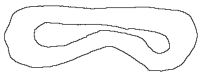
\includegraphics[interpolate=true,width=2.000000in,height=0.740000in]{contents/chapt7/figs/mass/mass_lap_2-img0.png}}%
\end{pgfscope}%
\begin{pgfscope}%
\pgfpathrectangle{\pgfqpoint{1.054417in}{3.947060in}}{\pgfqpoint{1.996630in}{0.737217in}}%
\pgfusepath{clip}%
\pgfsetbuttcap%
\pgfsetroundjoin%
\pgfsetlinewidth{1.505625pt}%
\definecolor{currentstroke}{rgb}{1.000000,0.000000,0.000000}%
\pgfsetstrokecolor{currentstroke}%
\pgfsetdash{{1.500000pt}{2.475000pt}}{0.000000pt}%
\pgfpathmoveto{\pgfqpoint{2.278748in}{4.381115in}}%
\pgfpathlineto{\pgfqpoint{2.278748in}{4.626854in}}%
\pgfusepath{stroke}%
\end{pgfscope}%
\begin{pgfscope}%
\pgfpathrectangle{\pgfqpoint{1.054417in}{3.947060in}}{\pgfqpoint{1.996630in}{0.737217in}}%
\pgfusepath{clip}%
\pgfsetrectcap%
\pgfsetroundjoin%
\pgfsetlinewidth{1.505625pt}%
\definecolor{currentstroke}{rgb}{0.121569,0.466667,0.705882}%
\pgfsetstrokecolor{currentstroke}%
\pgfsetstrokeopacity{0.700000}%
\pgfsetdash{}{0pt}%
\pgfpathmoveto{\pgfqpoint{2.283112in}{4.499973in}}%
\pgfpathlineto{\pgfqpoint{2.241212in}{4.500967in}}%
\pgfpathlineto{\pgfqpoint{2.208972in}{4.503980in}}%
\pgfpathlineto{\pgfqpoint{2.169935in}{4.510147in}}%
\pgfpathlineto{\pgfqpoint{2.098605in}{4.521320in}}%
\pgfpathlineto{\pgfqpoint{2.046990in}{4.527101in}}%
\pgfpathlineto{\pgfqpoint{2.004455in}{4.529806in}}%
\pgfpathlineto{\pgfqpoint{1.955058in}{4.530545in}}%
\pgfpathlineto{\pgfqpoint{1.825376in}{4.531098in}}%
\pgfpathlineto{\pgfqpoint{1.640222in}{4.537823in}}%
\pgfpathlineto{\pgfqpoint{1.547650in}{4.540943in}}%
\pgfpathlineto{\pgfqpoint{1.510637in}{4.539345in}}%
\pgfpathlineto{\pgfqpoint{1.479981in}{4.535694in}}%
\pgfpathlineto{\pgfqpoint{1.449751in}{4.529446in}}%
\pgfpathlineto{\pgfqpoint{1.426075in}{4.522417in}}%
\pgfpathlineto{\pgfqpoint{1.403039in}{4.513512in}}%
\pgfpathlineto{\pgfqpoint{1.380828in}{4.502715in}}%
\pgfpathlineto{\pgfqpoint{1.359653in}{4.490008in}}%
\pgfpathlineto{\pgfqpoint{1.339979in}{4.475092in}}%
\pgfpathlineto{\pgfqpoint{1.326544in}{4.462344in}}%
\pgfpathlineto{\pgfqpoint{1.314503in}{4.448272in}}%
\pgfpathlineto{\pgfqpoint{1.304115in}{4.432942in}}%
\pgfpathlineto{\pgfqpoint{1.295648in}{4.416474in}}%
\pgfpathlineto{\pgfqpoint{1.289317in}{4.399074in}}%
\pgfpathlineto{\pgfqpoint{1.285198in}{4.381021in}}%
\pgfpathlineto{\pgfqpoint{1.283344in}{4.362597in}}%
\pgfpathlineto{\pgfqpoint{1.283785in}{4.344085in}}%
\pgfpathlineto{\pgfqpoint{1.286470in}{4.325763in}}%
\pgfpathlineto{\pgfqpoint{1.291335in}{4.307895in}}%
\pgfpathlineto{\pgfqpoint{1.298269in}{4.290724in}}%
\pgfpathlineto{\pgfqpoint{1.307148in}{4.274472in}}%
\pgfpathlineto{\pgfqpoint{1.317678in}{4.259236in}}%
\pgfpathlineto{\pgfqpoint{1.329579in}{4.245043in}}%
\pgfpathlineto{\pgfqpoint{1.347271in}{4.227819in}}%
\pgfpathlineto{\pgfqpoint{1.366643in}{4.212503in}}%
\pgfpathlineto{\pgfqpoint{1.387322in}{4.199025in}}%
\pgfpathlineto{\pgfqpoint{1.414247in}{4.184424in}}%
\pgfpathlineto{\pgfqpoint{1.447368in}{4.169440in}}%
\pgfpathlineto{\pgfqpoint{1.486467in}{4.154490in}}%
\pgfpathlineto{\pgfqpoint{1.525120in}{4.141738in}}%
\pgfpathlineto{\pgfqpoint{1.552184in}{4.134932in}}%
\pgfpathlineto{\pgfqpoint{1.578785in}{4.130726in}}%
\pgfpathlineto{\pgfqpoint{1.599602in}{4.129606in}}%
\pgfpathlineto{\pgfqpoint{1.620591in}{4.130635in}}%
\pgfpathlineto{\pgfqpoint{1.647470in}{4.134562in}}%
\pgfpathlineto{\pgfqpoint{1.674899in}{4.140952in}}%
\pgfpathlineto{\pgfqpoint{1.702779in}{4.149507in}}%
\pgfpathlineto{\pgfqpoint{1.737088in}{4.162437in}}%
\pgfpathlineto{\pgfqpoint{1.782392in}{4.181903in}}%
\pgfpathlineto{\pgfqpoint{1.843620in}{4.211031in}}%
\pgfpathlineto{\pgfqpoint{1.899602in}{4.236820in}}%
\pgfpathlineto{\pgfqpoint{1.939678in}{4.252798in}}%
\pgfpathlineto{\pgfqpoint{1.974797in}{4.264376in}}%
\pgfpathlineto{\pgfqpoint{2.004607in}{4.272187in}}%
\pgfpathlineto{\pgfqpoint{2.034846in}{4.278120in}}%
\pgfpathlineto{\pgfqpoint{2.065412in}{4.282027in}}%
\pgfpathlineto{\pgfqpoint{2.096182in}{4.283649in}}%
\pgfpathlineto{\pgfqpoint{2.126984in}{4.282820in}}%
\pgfpathlineto{\pgfqpoint{2.157607in}{4.279421in}}%
\pgfpathlineto{\pgfqpoint{2.187823in}{4.273389in}}%
\pgfpathlineto{\pgfqpoint{2.223463in}{4.263524in}}%
\pgfpathlineto{\pgfqpoint{2.411774in}{4.204936in}}%
\pgfpathlineto{\pgfqpoint{2.445876in}{4.190640in}}%
\pgfpathlineto{\pgfqpoint{2.473406in}{4.176795in}}%
\pgfpathlineto{\pgfqpoint{2.499951in}{4.161145in}}%
\pgfpathlineto{\pgfqpoint{2.525353in}{4.143702in}}%
\pgfpathlineto{\pgfqpoint{2.554408in}{4.120824in}}%
\pgfpathlineto{\pgfqpoint{2.597739in}{4.086197in}}%
\pgfpathlineto{\pgfqpoint{2.618288in}{4.072584in}}%
\pgfpathlineto{\pgfqpoint{2.634404in}{4.063834in}}%
\pgfpathlineto{\pgfqpoint{2.651134in}{4.056899in}}%
\pgfpathlineto{\pgfqpoint{2.668379in}{4.052159in}}%
\pgfpathlineto{\pgfqpoint{2.685896in}{4.049927in}}%
\pgfpathlineto{\pgfqpoint{2.703319in}{4.050467in}}%
\pgfpathlineto{\pgfqpoint{2.720181in}{4.053895in}}%
\pgfpathlineto{\pgfqpoint{2.736070in}{4.060265in}}%
\pgfpathlineto{\pgfqpoint{2.751389in}{4.069725in}}%
\pgfpathlineto{\pgfqpoint{2.765961in}{4.081429in}}%
\pgfpathlineto{\pgfqpoint{2.783581in}{4.099047in}}%
\pgfpathlineto{\pgfqpoint{2.799143in}{4.118508in}}%
\pgfpathlineto{\pgfqpoint{2.812473in}{4.139561in}}%
\pgfpathlineto{\pgfqpoint{2.823345in}{4.161981in}}%
\pgfpathlineto{\pgfqpoint{2.831554in}{4.185506in}}%
\pgfpathlineto{\pgfqpoint{2.835865in}{4.203694in}}%
\pgfpathlineto{\pgfqpoint{2.839053in}{4.228406in}}%
\pgfpathlineto{\pgfqpoint{2.839486in}{4.247093in}}%
\pgfpathlineto{\pgfqpoint{2.838237in}{4.265743in}}%
\pgfpathlineto{\pgfqpoint{2.833992in}{4.290296in}}%
\pgfpathlineto{\pgfqpoint{2.826962in}{4.314201in}}%
\pgfpathlineto{\pgfqpoint{2.817280in}{4.337160in}}%
\pgfpathlineto{\pgfqpoint{2.805125in}{4.358913in}}%
\pgfpathlineto{\pgfqpoint{2.790690in}{4.379225in}}%
\pgfpathlineto{\pgfqpoint{2.774267in}{4.397970in}}%
\pgfpathlineto{\pgfqpoint{2.756252in}{4.415193in}}%
\pgfpathlineto{\pgfqpoint{2.736893in}{4.430891in}}%
\pgfpathlineto{\pgfqpoint{2.711170in}{4.448466in}}%
\pgfpathlineto{\pgfqpoint{2.684096in}{4.463881in}}%
\pgfpathlineto{\pgfqpoint{2.655996in}{4.477339in}}%
\pgfpathlineto{\pgfqpoint{2.627089in}{4.488968in}}%
\pgfpathlineto{\pgfqpoint{2.591582in}{4.500677in}}%
\pgfpathlineto{\pgfqpoint{2.555406in}{4.510128in}}%
\pgfpathlineto{\pgfqpoint{2.512641in}{4.518730in}}%
\pgfpathlineto{\pgfqpoint{2.469480in}{4.525065in}}%
\pgfpathlineto{\pgfqpoint{2.419854in}{4.529836in}}%
\pgfpathlineto{\pgfqpoint{2.370051in}{4.532123in}}%
\pgfpathlineto{\pgfqpoint{2.338890in}{4.532311in}}%
\pgfpathlineto{\pgfqpoint{2.338890in}{4.532311in}}%
\pgfusepath{stroke}%
\end{pgfscope}%
\begin{pgfscope}%
\pgfpathrectangle{\pgfqpoint{1.054417in}{3.947060in}}{\pgfqpoint{1.996630in}{0.737217in}}%
\pgfusepath{clip}%
\pgfsetrectcap%
\pgfsetroundjoin%
\pgfsetlinewidth{1.505625pt}%
\definecolor{currentstroke}{rgb}{1.000000,0.498039,0.054902}%
\pgfsetstrokecolor{currentstroke}%
\pgfsetstrokeopacity{0.700000}%
\pgfsetdash{}{0pt}%
\pgfpathmoveto{\pgfqpoint{2.283112in}{4.499973in}}%
\pgfpathlineto{\pgfqpoint{2.245234in}{4.500881in}}%
\pgfpathlineto{\pgfqpoint{2.217482in}{4.503690in}}%
\pgfpathlineto{\pgfqpoint{2.188687in}{4.508829in}}%
\pgfpathlineto{\pgfqpoint{2.107378in}{4.525087in}}%
\pgfpathlineto{\pgfqpoint{2.063572in}{4.531190in}}%
\pgfpathlineto{\pgfqpoint{2.023095in}{4.534482in}}%
\pgfpathlineto{\pgfqpoint{1.980691in}{4.535420in}}%
\pgfpathlineto{\pgfqpoint{1.900380in}{4.533683in}}%
\pgfpathlineto{\pgfqpoint{1.826235in}{4.532962in}}%
\pgfpathlineto{\pgfqpoint{1.764464in}{4.534507in}}%
\pgfpathlineto{\pgfqpoint{1.665730in}{4.539656in}}%
\pgfpathlineto{\pgfqpoint{1.585478in}{4.543054in}}%
\pgfpathlineto{\pgfqpoint{1.548414in}{4.542328in}}%
\pgfpathlineto{\pgfqpoint{1.517635in}{4.539707in}}%
\pgfpathlineto{\pgfqpoint{1.487140in}{4.534793in}}%
\pgfpathlineto{\pgfqpoint{1.457173in}{4.527308in}}%
\pgfpathlineto{\pgfqpoint{1.433761in}{4.519399in}}%
\pgfpathlineto{\pgfqpoint{1.411000in}{4.509776in}}%
\pgfpathlineto{\pgfqpoint{1.389027in}{4.498468in}}%
\pgfpathlineto{\pgfqpoint{1.368008in}{4.485477in}}%
\pgfpathlineto{\pgfqpoint{1.348369in}{4.470487in}}%
\pgfpathlineto{\pgfqpoint{1.334843in}{4.457819in}}%
\pgfpathlineto{\pgfqpoint{1.322568in}{4.443936in}}%
\pgfpathlineto{\pgfqpoint{1.311775in}{4.428874in}}%
\pgfpathlineto{\pgfqpoint{1.302717in}{4.412709in}}%
\pgfpathlineto{\pgfqpoint{1.295612in}{4.395598in}}%
\pgfpathlineto{\pgfqpoint{1.290584in}{4.377765in}}%
\pgfpathlineto{\pgfqpoint{1.287763in}{4.359453in}}%
\pgfpathlineto{\pgfqpoint{1.287208in}{4.340934in}}%
\pgfpathlineto{\pgfqpoint{1.288942in}{4.322488in}}%
\pgfpathlineto{\pgfqpoint{1.292923in}{4.304393in}}%
\pgfpathlineto{\pgfqpoint{1.299091in}{4.286922in}}%
\pgfpathlineto{\pgfqpoint{1.307282in}{4.270302in}}%
\pgfpathlineto{\pgfqpoint{1.317172in}{4.254630in}}%
\pgfpathlineto{\pgfqpoint{1.328537in}{4.239992in}}%
\pgfpathlineto{\pgfqpoint{1.345667in}{4.222192in}}%
\pgfpathlineto{\pgfqpoint{1.364638in}{4.206364in}}%
\pgfpathlineto{\pgfqpoint{1.385052in}{4.192468in}}%
\pgfpathlineto{\pgfqpoint{1.406523in}{4.180652in}}%
\pgfpathlineto{\pgfqpoint{1.428793in}{4.170984in}}%
\pgfpathlineto{\pgfqpoint{1.451667in}{4.163565in}}%
\pgfpathlineto{\pgfqpoint{1.474940in}{4.158503in}}%
\pgfpathlineto{\pgfqpoint{1.498425in}{4.155872in}}%
\pgfpathlineto{\pgfqpoint{1.522416in}{4.155426in}}%
\pgfpathlineto{\pgfqpoint{1.553035in}{4.157059in}}%
\pgfpathlineto{\pgfqpoint{1.595946in}{4.161963in}}%
\pgfpathlineto{\pgfqpoint{1.644689in}{4.169754in}}%
\pgfpathlineto{\pgfqpoint{1.686970in}{4.178574in}}%
\pgfpathlineto{\pgfqpoint{1.728711in}{4.189661in}}%
\pgfpathlineto{\pgfqpoint{1.769716in}{4.203227in}}%
\pgfpathlineto{\pgfqpoint{1.815740in}{4.221068in}}%
\pgfpathlineto{\pgfqpoint{1.872309in}{4.245713in}}%
\pgfpathlineto{\pgfqpoint{1.934750in}{4.272321in}}%
\pgfpathlineto{\pgfqpoint{1.975310in}{4.287159in}}%
\pgfpathlineto{\pgfqpoint{2.004968in}{4.295636in}}%
\pgfpathlineto{\pgfqpoint{2.029169in}{4.300456in}}%
\pgfpathlineto{\pgfqpoint{2.053694in}{4.303175in}}%
\pgfpathlineto{\pgfqpoint{2.078364in}{4.303442in}}%
\pgfpathlineto{\pgfqpoint{2.102922in}{4.301059in}}%
\pgfpathlineto{\pgfqpoint{2.127146in}{4.296360in}}%
\pgfpathlineto{\pgfqpoint{2.156889in}{4.288176in}}%
\pgfpathlineto{\pgfqpoint{2.263304in}{4.256450in}}%
\pgfpathlineto{\pgfqpoint{2.299525in}{4.248799in}}%
\pgfpathlineto{\pgfqpoint{2.342197in}{4.242125in}}%
\pgfpathlineto{\pgfqpoint{2.397099in}{4.233795in}}%
\pgfpathlineto{\pgfqpoint{2.427224in}{4.227161in}}%
\pgfpathlineto{\pgfqpoint{2.450838in}{4.220058in}}%
\pgfpathlineto{\pgfqpoint{2.473567in}{4.211145in}}%
\pgfpathlineto{\pgfqpoint{2.495107in}{4.200308in}}%
\pgfpathlineto{\pgfqpoint{2.515180in}{4.187498in}}%
\pgfpathlineto{\pgfqpoint{2.533530in}{4.172798in}}%
\pgfpathlineto{\pgfqpoint{2.550012in}{4.156284in}}%
\pgfpathlineto{\pgfqpoint{2.565541in}{4.137339in}}%
\pgfpathlineto{\pgfqpoint{2.622204in}{4.063649in}}%
\pgfpathlineto{\pgfqpoint{2.639305in}{4.047357in}}%
\pgfpathlineto{\pgfqpoint{2.652642in}{4.037660in}}%
\pgfpathlineto{\pgfqpoint{2.666352in}{4.030578in}}%
\pgfpathlineto{\pgfqpoint{2.680163in}{4.026605in}}%
\pgfpathlineto{\pgfqpoint{2.689142in}{4.025912in}}%
\pgfpathlineto{\pgfqpoint{2.697625in}{4.026863in}}%
\pgfpathlineto{\pgfqpoint{2.705275in}{4.029423in}}%
\pgfpathlineto{\pgfqpoint{2.711732in}{4.033686in}}%
\pgfpathlineto{\pgfqpoint{2.716688in}{4.039831in}}%
\pgfpathlineto{\pgfqpoint{2.720133in}{4.047106in}}%
\pgfpathlineto{\pgfqpoint{2.723041in}{4.059106in}}%
\pgfpathlineto{\pgfqpoint{2.724229in}{4.076055in}}%
\pgfpathlineto{\pgfqpoint{2.723345in}{4.111812in}}%
\pgfpathlineto{\pgfqpoint{2.723452in}{4.142227in}}%
\pgfpathlineto{\pgfqpoint{2.726103in}{4.161868in}}%
\pgfpathlineto{\pgfqpoint{2.730114in}{4.176092in}}%
\pgfpathlineto{\pgfqpoint{2.736129in}{4.189383in}}%
\pgfpathlineto{\pgfqpoint{2.746603in}{4.205576in}}%
\pgfpathlineto{\pgfqpoint{2.765285in}{4.228972in}}%
\pgfpathlineto{\pgfqpoint{2.794102in}{4.261413in}}%
\pgfpathlineto{\pgfqpoint{2.821948in}{4.293118in}}%
\pgfpathlineto{\pgfqpoint{2.834111in}{4.310675in}}%
\pgfpathlineto{\pgfqpoint{2.841277in}{4.325004in}}%
\pgfpathlineto{\pgfqpoint{2.845774in}{4.339337in}}%
\pgfpathlineto{\pgfqpoint{2.847312in}{4.353873in}}%
\pgfpathlineto{\pgfqpoint{2.846032in}{4.368439in}}%
\pgfpathlineto{\pgfqpoint{2.842236in}{4.382563in}}%
\pgfpathlineto{\pgfqpoint{2.836187in}{4.395880in}}%
\pgfpathlineto{\pgfqpoint{2.828142in}{4.408110in}}%
\pgfpathlineto{\pgfqpoint{2.818382in}{4.419058in}}%
\pgfpathlineto{\pgfqpoint{2.807121in}{4.428498in}}%
\pgfpathlineto{\pgfqpoint{2.794602in}{4.436248in}}%
\pgfpathlineto{\pgfqpoint{2.781085in}{4.442152in}}%
\pgfpathlineto{\pgfqpoint{2.766563in}{4.446194in}}%
\pgfpathlineto{\pgfqpoint{2.746805in}{4.449221in}}%
\pgfpathlineto{\pgfqpoint{2.716749in}{4.451248in}}%
\pgfpathlineto{\pgfqpoint{2.646228in}{4.455386in}}%
\pgfpathlineto{\pgfqpoint{2.622470in}{4.459807in}}%
\pgfpathlineto{\pgfqpoint{2.603732in}{4.465235in}}%
\pgfpathlineto{\pgfqpoint{2.585185in}{4.472640in}}%
\pgfpathlineto{\pgfqpoint{2.561678in}{4.484541in}}%
\pgfpathlineto{\pgfqpoint{2.457737in}{4.541439in}}%
\pgfpathlineto{\pgfqpoint{2.434878in}{4.550333in}}%
\pgfpathlineto{\pgfqpoint{2.411329in}{4.557202in}}%
\pgfpathlineto{\pgfqpoint{2.387203in}{4.561657in}}%
\pgfpathlineto{\pgfqpoint{2.362556in}{4.563572in}}%
\pgfpathlineto{\pgfqpoint{2.337835in}{4.563297in}}%
\pgfpathlineto{\pgfqpoint{2.313218in}{4.560999in}}%
\pgfpathlineto{\pgfqpoint{2.282782in}{4.555640in}}%
\pgfpathlineto{\pgfqpoint{2.282782in}{4.555640in}}%
\pgfusepath{stroke}%
\end{pgfscope}%
\begin{pgfscope}%
\pgfsetbuttcap%
\pgfsetmiterjoin%
\definecolor{currentfill}{rgb}{1.000000,1.000000,1.000000}%
\pgfsetfillcolor{currentfill}%
\pgfsetlinewidth{1.003750pt}%
\definecolor{currentstroke}{rgb}{0.000000,0.000000,0.000000}%
\pgfsetstrokecolor{currentstroke}%
\pgfsetdash{}{0pt}%
\pgfpathmoveto{\pgfqpoint{1.518815in}{4.500306in}}%
\pgfpathlineto{\pgfqpoint{1.775964in}{4.500306in}}%
\pgfpathquadraticcurveto{\pgfqpoint{1.787534in}{4.500306in}}{\pgfqpoint{1.787534in}{4.511875in}}%
\pgfpathlineto{\pgfqpoint{1.787534in}{4.623841in}}%
\pgfpathquadraticcurveto{\pgfqpoint{1.787534in}{4.635410in}}{\pgfqpoint{1.775964in}{4.635410in}}%
\pgfpathlineto{\pgfqpoint{1.518815in}{4.635410in}}%
\pgfpathquadraticcurveto{\pgfqpoint{1.507246in}{4.635410in}}{\pgfqpoint{1.507246in}{4.623841in}}%
\pgfpathlineto{\pgfqpoint{1.507246in}{4.511875in}}%
\pgfpathquadraticcurveto{\pgfqpoint{1.507246in}{4.500306in}}{\pgfqpoint{1.518815in}{4.500306in}}%
\pgfpathlineto{\pgfqpoint{1.518815in}{4.500306in}}%
\pgfpathclose%
\pgfusepath{stroke,fill}%
\end{pgfscope}%
\begin{pgfscope}%
\definecolor{textcolor}{rgb}{0.000000,0.000000,0.000000}%
\pgfsetstrokecolor{textcolor}%
\pgfsetfillcolor{textcolor}%
\pgftext[x=1.518815in,y=4.535940in,left,base]{\color{textcolor}\rmfamily\fontsize{8.330000}{9.996000}\selectfont 20\%}%
\end{pgfscope}%
\begin{pgfscope}%
\pgfsetbuttcap%
\pgfsetmiterjoin%
\definecolor{currentfill}{rgb}{1.000000,1.000000,1.000000}%
\pgfsetfillcolor{currentfill}%
\pgfsetlinewidth{1.003750pt}%
\definecolor{currentstroke}{rgb}{0.000000,0.000000,0.000000}%
\pgfsetstrokecolor{currentstroke}%
\pgfsetdash{}{0pt}%
\pgfpathmoveto{\pgfqpoint{1.516473in}{4.083711in}}%
\pgfpathlineto{\pgfqpoint{1.773622in}{4.083711in}}%
\pgfpathquadraticcurveto{\pgfqpoint{1.785192in}{4.083711in}}{\pgfqpoint{1.785192in}{4.095280in}}%
\pgfpathlineto{\pgfqpoint{1.785192in}{4.207246in}}%
\pgfpathquadraticcurveto{\pgfqpoint{1.785192in}{4.218815in}}{\pgfqpoint{1.773622in}{4.218815in}}%
\pgfpathlineto{\pgfqpoint{1.516473in}{4.218815in}}%
\pgfpathquadraticcurveto{\pgfqpoint{1.504904in}{4.218815in}}{\pgfqpoint{1.504904in}{4.207246in}}%
\pgfpathlineto{\pgfqpoint{1.504904in}{4.095280in}}%
\pgfpathquadraticcurveto{\pgfqpoint{1.504904in}{4.083711in}}{\pgfqpoint{1.516473in}{4.083711in}}%
\pgfpathlineto{\pgfqpoint{1.516473in}{4.083711in}}%
\pgfpathclose%
\pgfusepath{stroke,fill}%
\end{pgfscope}%
\begin{pgfscope}%
\definecolor{textcolor}{rgb}{0.000000,0.000000,0.000000}%
\pgfsetstrokecolor{textcolor}%
\pgfsetfillcolor{textcolor}%
\pgftext[x=1.516473in,y=4.119345in,left,base]{\color{textcolor}\rmfamily\fontsize{8.330000}{9.996000}\selectfont 40\%}%
\end{pgfscope}%
\begin{pgfscope}%
\pgfsetbuttcap%
\pgfsetmiterjoin%
\definecolor{currentfill}{rgb}{1.000000,1.000000,1.000000}%
\pgfsetfillcolor{currentfill}%
\pgfsetlinewidth{1.003750pt}%
\definecolor{currentstroke}{rgb}{0.000000,0.000000,0.000000}%
\pgfsetstrokecolor{currentstroke}%
\pgfsetdash{}{0pt}%
\pgfpathmoveto{\pgfqpoint{2.243577in}{4.244496in}}%
\pgfpathlineto{\pgfqpoint{2.500726in}{4.244496in}}%
\pgfpathquadraticcurveto{\pgfqpoint{2.512295in}{4.244496in}}{\pgfqpoint{2.512295in}{4.256065in}}%
\pgfpathlineto{\pgfqpoint{2.512295in}{4.368031in}}%
\pgfpathquadraticcurveto{\pgfqpoint{2.512295in}{4.379600in}}{\pgfqpoint{2.500726in}{4.379600in}}%
\pgfpathlineto{\pgfqpoint{2.243577in}{4.379600in}}%
\pgfpathquadraticcurveto{\pgfqpoint{2.232007in}{4.379600in}}{\pgfqpoint{2.232007in}{4.368031in}}%
\pgfpathlineto{\pgfqpoint{2.232007in}{4.256065in}}%
\pgfpathquadraticcurveto{\pgfqpoint{2.232007in}{4.244496in}}{\pgfqpoint{2.243577in}{4.244496in}}%
\pgfpathlineto{\pgfqpoint{2.243577in}{4.244496in}}%
\pgfpathclose%
\pgfusepath{stroke,fill}%
\end{pgfscope}%
\begin{pgfscope}%
\definecolor{textcolor}{rgb}{0.000000,0.000000,0.000000}%
\pgfsetstrokecolor{textcolor}%
\pgfsetfillcolor{textcolor}%
\pgftext[x=2.243577in,y=4.280130in,left,base]{\color{textcolor}\rmfamily\fontsize{8.330000}{9.996000}\selectfont 60\%}%
\end{pgfscope}%
\begin{pgfscope}%
\pgfsetbuttcap%
\pgfsetmiterjoin%
\definecolor{currentfill}{rgb}{1.000000,1.000000,1.000000}%
\pgfsetfillcolor{currentfill}%
\pgfsetlinewidth{1.003750pt}%
\definecolor{currentstroke}{rgb}{0.000000,0.000000,0.000000}%
\pgfsetstrokecolor{currentstroke}%
\pgfsetdash{}{0pt}%
\pgfpathmoveto{\pgfqpoint{2.864174in}{4.190295in}}%
\pgfpathlineto{\pgfqpoint{3.121323in}{4.190295in}}%
\pgfpathquadraticcurveto{\pgfqpoint{3.132892in}{4.190295in}}{\pgfqpoint{3.132892in}{4.201865in}}%
\pgfpathlineto{\pgfqpoint{3.132892in}{4.313830in}}%
\pgfpathquadraticcurveto{\pgfqpoint{3.132892in}{4.325400in}}{\pgfqpoint{3.121323in}{4.325400in}}%
\pgfpathlineto{\pgfqpoint{2.864174in}{4.325400in}}%
\pgfpathquadraticcurveto{\pgfqpoint{2.852605in}{4.325400in}}{\pgfqpoint{2.852605in}{4.313830in}}%
\pgfpathlineto{\pgfqpoint{2.852605in}{4.201865in}}%
\pgfpathquadraticcurveto{\pgfqpoint{2.852605in}{4.190295in}}{\pgfqpoint{2.864174in}{4.190295in}}%
\pgfpathlineto{\pgfqpoint{2.864174in}{4.190295in}}%
\pgfpathclose%
\pgfusepath{stroke,fill}%
\end{pgfscope}%
\begin{pgfscope}%
\definecolor{textcolor}{rgb}{0.000000,0.000000,0.000000}%
\pgfsetstrokecolor{textcolor}%
\pgfsetfillcolor{textcolor}%
\pgftext[x=2.864174in,y=4.225930in,left,base]{\color{textcolor}\rmfamily\fontsize{8.330000}{9.996000}\selectfont 80\%}%
\end{pgfscope}%
\begin{pgfscope}%
\definecolor{textcolor}{rgb}{0.000000,0.000000,0.000000}%
\pgfsetstrokecolor{textcolor}%
\pgfsetfillcolor{textcolor}%
\pgftext[x=2.052732in,y=4.767611in,,base]{\color{textcolor}\rmfamily\fontsize{12.000000}{14.400000}\selectfont End-to-end}%
\end{pgfscope}%
\begin{pgfscope}%
\pgfpathrectangle{\pgfqpoint{3.277208in}{3.947060in}}{\pgfqpoint{1.996630in}{0.737217in}}%
\pgfusepath{clip}%
\pgfsys@transformshift{3.277208in}{3.947060in}%
\pgftext[left,bottom]{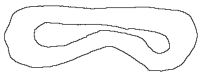
\includegraphics[interpolate=true,width=2.000000in,height=0.740000in]{contents/chapt7/figs/mass/mass_lap_2-img1.png}}%
\end{pgfscope}%
\begin{pgfscope}%
\pgfpathrectangle{\pgfqpoint{3.277208in}{3.947060in}}{\pgfqpoint{1.996630in}{0.737217in}}%
\pgfusepath{clip}%
\pgfsetbuttcap%
\pgfsetroundjoin%
\pgfsetlinewidth{1.505625pt}%
\definecolor{currentstroke}{rgb}{1.000000,0.000000,0.000000}%
\pgfsetstrokecolor{currentstroke}%
\pgfsetdash{{1.500000pt}{2.475000pt}}{0.000000pt}%
\pgfpathmoveto{\pgfqpoint{4.501540in}{4.381115in}}%
\pgfpathlineto{\pgfqpoint{4.501540in}{4.626854in}}%
\pgfusepath{stroke}%
\end{pgfscope}%
\begin{pgfscope}%
\pgfpathrectangle{\pgfqpoint{3.277208in}{3.947060in}}{\pgfqpoint{1.996630in}{0.737217in}}%
\pgfusepath{clip}%
\pgfsetrectcap%
\pgfsetroundjoin%
\pgfsetlinewidth{1.505625pt}%
\definecolor{currentstroke}{rgb}{0.121569,0.466667,0.705882}%
\pgfsetstrokecolor{currentstroke}%
\pgfsetstrokeopacity{0.700000}%
\pgfsetdash{}{0pt}%
\pgfpathmoveto{\pgfqpoint{4.505904in}{4.499973in}}%
\pgfpathlineto{\pgfqpoint{4.439235in}{4.500939in}}%
\pgfpathlineto{\pgfqpoint{4.262395in}{4.505960in}}%
\pgfpathlineto{\pgfqpoint{4.177660in}{4.504187in}}%
\pgfpathlineto{\pgfqpoint{4.042903in}{4.501442in}}%
\pgfpathlineto{\pgfqpoint{3.889485in}{4.499449in}}%
\pgfpathlineto{\pgfqpoint{3.834380in}{4.496010in}}%
\pgfpathlineto{\pgfqpoint{3.785562in}{4.490753in}}%
\pgfpathlineto{\pgfqpoint{3.736987in}{4.483161in}}%
\pgfpathlineto{\pgfqpoint{3.700945in}{4.475479in}}%
\pgfpathlineto{\pgfqpoint{3.671359in}{4.467202in}}%
\pgfpathlineto{\pgfqpoint{3.642503in}{4.456668in}}%
\pgfpathlineto{\pgfqpoint{3.620240in}{4.446188in}}%
\pgfpathlineto{\pgfqpoint{3.599105in}{4.433651in}}%
\pgfpathlineto{\pgfqpoint{3.579444in}{4.418882in}}%
\pgfpathlineto{\pgfqpoint{3.565977in}{4.406382in}}%
\pgfpathlineto{\pgfqpoint{3.553929in}{4.392750in}}%
\pgfpathlineto{\pgfqpoint{3.543489in}{4.378042in}}%
\pgfpathlineto{\pgfqpoint{3.534827in}{4.362348in}}%
\pgfpathlineto{\pgfqpoint{3.528121in}{4.345835in}}%
\pgfpathlineto{\pgfqpoint{3.523483in}{4.328735in}}%
\pgfpathlineto{\pgfqpoint{3.521002in}{4.311321in}}%
\pgfpathlineto{\pgfqpoint{3.520658in}{4.293665in}}%
\pgfpathlineto{\pgfqpoint{3.522382in}{4.275992in}}%
\pgfpathlineto{\pgfqpoint{3.526113in}{4.258582in}}%
\pgfpathlineto{\pgfqpoint{3.531750in}{4.241612in}}%
\pgfpathlineto{\pgfqpoint{3.539204in}{4.225228in}}%
\pgfpathlineto{\pgfqpoint{3.548359in}{4.209612in}}%
\pgfpathlineto{\pgfqpoint{3.559021in}{4.194959in}}%
\pgfpathlineto{\pgfqpoint{3.571119in}{4.181372in}}%
\pgfpathlineto{\pgfqpoint{3.584534in}{4.168887in}}%
\pgfpathlineto{\pgfqpoint{3.604113in}{4.154203in}}%
\pgfpathlineto{\pgfqpoint{3.625275in}{4.141958in}}%
\pgfpathlineto{\pgfqpoint{3.647825in}{4.132260in}}%
\pgfpathlineto{\pgfqpoint{3.671348in}{4.125212in}}%
\pgfpathlineto{\pgfqpoint{3.695474in}{4.120504in}}%
\pgfpathlineto{\pgfqpoint{3.719915in}{4.117965in}}%
\pgfpathlineto{\pgfqpoint{3.744463in}{4.117383in}}%
\pgfpathlineto{\pgfqpoint{3.775138in}{4.119096in}}%
\pgfpathlineto{\pgfqpoint{3.805576in}{4.123241in}}%
\pgfpathlineto{\pgfqpoint{3.835588in}{4.129640in}}%
\pgfpathlineto{\pgfqpoint{3.865091in}{4.138195in}}%
\pgfpathlineto{\pgfqpoint{3.893914in}{4.148803in}}%
\pgfpathlineto{\pgfqpoint{3.927661in}{4.163714in}}%
\pgfpathlineto{\pgfqpoint{3.994839in}{4.194020in}}%
\pgfpathlineto{\pgfqpoint{4.029428in}{4.206696in}}%
\pgfpathlineto{\pgfqpoint{4.064669in}{4.217242in}}%
\pgfpathlineto{\pgfqpoint{4.106511in}{4.227086in}}%
\pgfpathlineto{\pgfqpoint{4.148784in}{4.234710in}}%
\pgfpathlineto{\pgfqpoint{4.191344in}{4.240380in}}%
\pgfpathlineto{\pgfqpoint{4.240292in}{4.244579in}}%
\pgfpathlineto{\pgfqpoint{4.283266in}{4.245961in}}%
\pgfpathlineto{\pgfqpoint{4.320111in}{4.245162in}}%
\pgfpathlineto{\pgfqpoint{4.356760in}{4.242337in}}%
\pgfpathlineto{\pgfqpoint{4.393197in}{4.237411in}}%
\pgfpathlineto{\pgfqpoint{4.435419in}{4.229334in}}%
\pgfpathlineto{\pgfqpoint{4.477215in}{4.219068in}}%
\pgfpathlineto{\pgfqpoint{4.524262in}{4.204880in}}%
\pgfpathlineto{\pgfqpoint{4.699980in}{4.149562in}}%
\pgfpathlineto{\pgfqpoint{4.747362in}{4.136821in}}%
\pgfpathlineto{\pgfqpoint{4.783303in}{4.129279in}}%
\pgfpathlineto{\pgfqpoint{4.813572in}{4.125033in}}%
\pgfpathlineto{\pgfqpoint{4.844180in}{4.123162in}}%
\pgfpathlineto{\pgfqpoint{4.868732in}{4.123658in}}%
\pgfpathlineto{\pgfqpoint{4.893155in}{4.126191in}}%
\pgfpathlineto{\pgfqpoint{4.917262in}{4.130914in}}%
\pgfpathlineto{\pgfqpoint{4.940738in}{4.138010in}}%
\pgfpathlineto{\pgfqpoint{4.963363in}{4.147579in}}%
\pgfpathlineto{\pgfqpoint{4.984788in}{4.159634in}}%
\pgfpathlineto{\pgfqpoint{4.999812in}{4.170306in}}%
\pgfpathlineto{\pgfqpoint{5.013778in}{4.182312in}}%
\pgfpathlineto{\pgfqpoint{5.026527in}{4.195598in}}%
\pgfpathlineto{\pgfqpoint{5.037874in}{4.210120in}}%
\pgfpathlineto{\pgfqpoint{5.047660in}{4.225730in}}%
\pgfpathlineto{\pgfqpoint{5.055714in}{4.242251in}}%
\pgfpathlineto{\pgfqpoint{5.061856in}{4.259369in}}%
\pgfpathlineto{\pgfqpoint{5.065941in}{4.276899in}}%
\pgfpathlineto{\pgfqpoint{5.067864in}{4.294676in}}%
\pgfpathlineto{\pgfqpoint{5.067555in}{4.312468in}}%
\pgfpathlineto{\pgfqpoint{5.065041in}{4.329950in}}%
\pgfpathlineto{\pgfqpoint{5.060369in}{4.346916in}}%
\pgfpathlineto{\pgfqpoint{5.053660in}{4.363238in}}%
\pgfpathlineto{\pgfqpoint{5.045087in}{4.378715in}}%
\pgfpathlineto{\pgfqpoint{5.034847in}{4.393209in}}%
\pgfpathlineto{\pgfqpoint{5.023172in}{4.406634in}}%
\pgfpathlineto{\pgfqpoint{5.010234in}{4.418911in}}%
\pgfpathlineto{\pgfqpoint{4.991311in}{4.433341in}}%
\pgfpathlineto{\pgfqpoint{4.970813in}{4.445558in}}%
\pgfpathlineto{\pgfqpoint{4.949040in}{4.455666in}}%
\pgfpathlineto{\pgfqpoint{4.926270in}{4.463823in}}%
\pgfpathlineto{\pgfqpoint{4.902802in}{4.470120in}}%
\pgfpathlineto{\pgfqpoint{4.878892in}{4.474640in}}%
\pgfpathlineto{\pgfqpoint{4.848641in}{4.478093in}}%
\pgfpathlineto{\pgfqpoint{4.744815in}{4.487216in}}%
\pgfpathlineto{\pgfqpoint{4.702495in}{4.494905in}}%
\pgfpathlineto{\pgfqpoint{4.630570in}{4.511018in}}%
\pgfpathlineto{\pgfqpoint{4.582464in}{4.520895in}}%
\pgfpathlineto{\pgfqpoint{4.552040in}{4.525064in}}%
\pgfpathlineto{\pgfqpoint{4.521428in}{4.527073in}}%
\pgfpathlineto{\pgfqpoint{4.515292in}{4.527175in}}%
\pgfpathlineto{\pgfqpoint{4.515292in}{4.527175in}}%
\pgfusepath{stroke}%
\end{pgfscope}%
\begin{pgfscope}%
\pgfpathrectangle{\pgfqpoint{3.277208in}{3.947060in}}{\pgfqpoint{1.996630in}{0.737217in}}%
\pgfusepath{clip}%
\pgfsetrectcap%
\pgfsetroundjoin%
\pgfsetlinewidth{1.505625pt}%
\definecolor{currentstroke}{rgb}{1.000000,0.498039,0.054902}%
\pgfsetstrokecolor{currentstroke}%
\pgfsetstrokeopacity{0.700000}%
\pgfsetdash{}{0pt}%
\pgfpathmoveto{\pgfqpoint{4.505904in}{4.499973in}}%
\pgfpathlineto{\pgfqpoint{4.412619in}{4.500955in}}%
\pgfpathlineto{\pgfqpoint{4.232301in}{4.505480in}}%
\pgfpathlineto{\pgfqpoint{4.159524in}{4.504345in}}%
\pgfpathlineto{\pgfqpoint{4.031261in}{4.501469in}}%
\pgfpathlineto{\pgfqpoint{3.902494in}{4.500042in}}%
\pgfpathlineto{\pgfqpoint{3.847346in}{4.496531in}}%
\pgfpathlineto{\pgfqpoint{3.798451in}{4.491087in}}%
\pgfpathlineto{\pgfqpoint{3.749912in}{4.483287in}}%
\pgfpathlineto{\pgfqpoint{3.707854in}{4.474126in}}%
\pgfpathlineto{\pgfqpoint{3.678311in}{4.465748in}}%
\pgfpathlineto{\pgfqpoint{3.649450in}{4.455261in}}%
\pgfpathlineto{\pgfqpoint{3.627163in}{4.444963in}}%
\pgfpathlineto{\pgfqpoint{3.605896in}{4.432666in}}%
\pgfpathlineto{\pgfqpoint{3.586057in}{4.418181in}}%
\pgfpathlineto{\pgfqpoint{3.572380in}{4.405851in}}%
\pgfpathlineto{\pgfqpoint{3.560103in}{4.392367in}}%
\pgfpathlineto{\pgfqpoint{3.549448in}{4.377810in}}%
\pgfpathlineto{\pgfqpoint{3.540623in}{4.362276in}}%
\pgfpathlineto{\pgfqpoint{3.533847in}{4.345914in}}%
\pgfpathlineto{\pgfqpoint{3.529266in}{4.328918in}}%
\pgfpathlineto{\pgfqpoint{3.526988in}{4.311578in}}%
\pgfpathlineto{\pgfqpoint{3.526976in}{4.294089in}}%
\pgfpathlineto{\pgfqpoint{3.529202in}{4.276565in}}%
\pgfpathlineto{\pgfqpoint{3.533503in}{4.259284in}}%
\pgfpathlineto{\pgfqpoint{3.539720in}{4.242415in}}%
\pgfpathlineto{\pgfqpoint{3.547657in}{4.226169in}}%
\pgfpathlineto{\pgfqpoint{3.557191in}{4.210696in}}%
\pgfpathlineto{\pgfqpoint{3.568192in}{4.196148in}}%
\pgfpathlineto{\pgfqpoint{3.580542in}{4.182679in}}%
\pgfpathlineto{\pgfqpoint{3.594146in}{4.170339in}}%
\pgfpathlineto{\pgfqpoint{3.608814in}{4.159303in}}%
\pgfpathlineto{\pgfqpoint{3.624474in}{4.149651in}}%
\pgfpathlineto{\pgfqpoint{3.640971in}{4.141474in}}%
\pgfpathlineto{\pgfqpoint{3.664009in}{4.132879in}}%
\pgfpathlineto{\pgfqpoint{3.687883in}{4.126994in}}%
\pgfpathlineto{\pgfqpoint{3.712188in}{4.123555in}}%
\pgfpathlineto{\pgfqpoint{3.736700in}{4.122398in}}%
\pgfpathlineto{\pgfqpoint{3.761252in}{4.123337in}}%
\pgfpathlineto{\pgfqpoint{3.791689in}{4.127101in}}%
\pgfpathlineto{\pgfqpoint{3.821779in}{4.133276in}}%
\pgfpathlineto{\pgfqpoint{3.851385in}{4.141528in}}%
\pgfpathlineto{\pgfqpoint{3.886161in}{4.153706in}}%
\pgfpathlineto{\pgfqpoint{3.920168in}{4.167858in}}%
\pgfpathlineto{\pgfqpoint{3.993505in}{4.199359in}}%
\pgfpathlineto{\pgfqpoint{4.028384in}{4.211380in}}%
\pgfpathlineto{\pgfqpoint{4.063996in}{4.221086in}}%
\pgfpathlineto{\pgfqpoint{4.100020in}{4.228757in}}%
\pgfpathlineto{\pgfqpoint{4.142458in}{4.235458in}}%
\pgfpathlineto{\pgfqpoint{4.197420in}{4.241563in}}%
\pgfpathlineto{\pgfqpoint{4.246433in}{4.244822in}}%
\pgfpathlineto{\pgfqpoint{4.289357in}{4.245691in}}%
\pgfpathlineto{\pgfqpoint{4.332306in}{4.244188in}}%
\pgfpathlineto{\pgfqpoint{4.368921in}{4.240735in}}%
\pgfpathlineto{\pgfqpoint{4.405222in}{4.235128in}}%
\pgfpathlineto{\pgfqpoint{4.447225in}{4.226401in}}%
\pgfpathlineto{\pgfqpoint{4.494821in}{4.214262in}}%
\pgfpathlineto{\pgfqpoint{4.559642in}{4.195167in}}%
\pgfpathlineto{\pgfqpoint{4.759658in}{4.134994in}}%
\pgfpathlineto{\pgfqpoint{4.789773in}{4.129001in}}%
\pgfpathlineto{\pgfqpoint{4.820262in}{4.125064in}}%
\pgfpathlineto{\pgfqpoint{4.850978in}{4.123717in}}%
\pgfpathlineto{\pgfqpoint{4.875552in}{4.124783in}}%
\pgfpathlineto{\pgfqpoint{4.899905in}{4.128012in}}%
\pgfpathlineto{\pgfqpoint{4.923824in}{4.133540in}}%
\pgfpathlineto{\pgfqpoint{4.947000in}{4.141553in}}%
\pgfpathlineto{\pgfqpoint{4.969203in}{4.152125in}}%
\pgfpathlineto{\pgfqpoint{4.984907in}{4.161676in}}%
\pgfpathlineto{\pgfqpoint{4.999385in}{4.172487in}}%
\pgfpathlineto{\pgfqpoint{5.012473in}{4.184538in}}%
\pgfpathlineto{\pgfqpoint{5.023979in}{4.197780in}}%
\pgfpathlineto{\pgfqpoint{5.033689in}{4.212119in}}%
\pgfpathlineto{\pgfqpoint{5.041438in}{4.227387in}}%
\pgfpathlineto{\pgfqpoint{5.047091in}{4.243370in}}%
\pgfpathlineto{\pgfqpoint{5.050591in}{4.259808in}}%
\pgfpathlineto{\pgfqpoint{5.051977in}{4.276439in}}%
\pgfpathlineto{\pgfqpoint{5.051287in}{4.293018in}}%
\pgfpathlineto{\pgfqpoint{5.048664in}{4.309308in}}%
\pgfpathlineto{\pgfqpoint{5.044217in}{4.325105in}}%
\pgfpathlineto{\pgfqpoint{5.038087in}{4.340255in}}%
\pgfpathlineto{\pgfqpoint{5.030395in}{4.354642in}}%
\pgfpathlineto{\pgfqpoint{5.017735in}{4.372811in}}%
\pgfpathlineto{\pgfqpoint{5.002640in}{4.389783in}}%
\pgfpathlineto{\pgfqpoint{4.985505in}{4.405419in}}%
\pgfpathlineto{\pgfqpoint{4.966696in}{4.419603in}}%
\pgfpathlineto{\pgfqpoint{4.946488in}{4.432172in}}%
\pgfpathlineto{\pgfqpoint{4.925031in}{4.443035in}}%
\pgfpathlineto{\pgfqpoint{4.902636in}{4.452219in}}%
\pgfpathlineto{\pgfqpoint{4.879499in}{4.459648in}}%
\pgfpathlineto{\pgfqpoint{4.849736in}{4.466543in}}%
\pgfpathlineto{\pgfqpoint{4.819503in}{4.470937in}}%
\pgfpathlineto{\pgfqpoint{4.776866in}{4.474326in}}%
\pgfpathlineto{\pgfqpoint{4.721803in}{4.479033in}}%
\pgfpathlineto{\pgfqpoint{4.691425in}{4.483647in}}%
\pgfpathlineto{\pgfqpoint{4.655407in}{4.491346in}}%
\pgfpathlineto{\pgfqpoint{4.607908in}{4.503816in}}%
\pgfpathlineto{\pgfqpoint{4.548472in}{4.519435in}}%
\pgfpathlineto{\pgfqpoint{4.518246in}{4.525256in}}%
\pgfpathlineto{\pgfqpoint{4.506064in}{4.526991in}}%
\pgfpathlineto{\pgfqpoint{4.506064in}{4.526991in}}%
\pgfusepath{stroke}%
\end{pgfscope}%
\begin{pgfscope}%
\pgfsetbuttcap%
\pgfsetmiterjoin%
\definecolor{currentfill}{rgb}{1.000000,1.000000,1.000000}%
\pgfsetfillcolor{currentfill}%
\pgfsetlinewidth{1.003750pt}%
\definecolor{currentstroke}{rgb}{0.000000,0.000000,0.000000}%
\pgfsetstrokecolor{currentstroke}%
\pgfsetdash{}{0pt}%
\pgfpathmoveto{\pgfqpoint{3.741607in}{4.500306in}}%
\pgfpathlineto{\pgfqpoint{3.998756in}{4.500306in}}%
\pgfpathquadraticcurveto{\pgfqpoint{4.010325in}{4.500306in}}{\pgfqpoint{4.010325in}{4.511875in}}%
\pgfpathlineto{\pgfqpoint{4.010325in}{4.623841in}}%
\pgfpathquadraticcurveto{\pgfqpoint{4.010325in}{4.635410in}}{\pgfqpoint{3.998756in}{4.635410in}}%
\pgfpathlineto{\pgfqpoint{3.741607in}{4.635410in}}%
\pgfpathquadraticcurveto{\pgfqpoint{3.730037in}{4.635410in}}{\pgfqpoint{3.730037in}{4.623841in}}%
\pgfpathlineto{\pgfqpoint{3.730037in}{4.511875in}}%
\pgfpathquadraticcurveto{\pgfqpoint{3.730037in}{4.500306in}}{\pgfqpoint{3.741607in}{4.500306in}}%
\pgfpathlineto{\pgfqpoint{3.741607in}{4.500306in}}%
\pgfpathclose%
\pgfusepath{stroke,fill}%
\end{pgfscope}%
\begin{pgfscope}%
\definecolor{textcolor}{rgb}{0.000000,0.000000,0.000000}%
\pgfsetstrokecolor{textcolor}%
\pgfsetfillcolor{textcolor}%
\pgftext[x=3.741607in,y=4.535940in,left,base]{\color{textcolor}\rmfamily\fontsize{8.330000}{9.996000}\selectfont 20\%}%
\end{pgfscope}%
\begin{pgfscope}%
\pgfsetbuttcap%
\pgfsetmiterjoin%
\definecolor{currentfill}{rgb}{1.000000,1.000000,1.000000}%
\pgfsetfillcolor{currentfill}%
\pgfsetlinewidth{1.003750pt}%
\definecolor{currentstroke}{rgb}{0.000000,0.000000,0.000000}%
\pgfsetstrokecolor{currentstroke}%
\pgfsetdash{}{0pt}%
\pgfpathmoveto{\pgfqpoint{3.739265in}{4.083711in}}%
\pgfpathlineto{\pgfqpoint{3.996414in}{4.083711in}}%
\pgfpathquadraticcurveto{\pgfqpoint{4.007983in}{4.083711in}}{\pgfqpoint{4.007983in}{4.095280in}}%
\pgfpathlineto{\pgfqpoint{4.007983in}{4.207246in}}%
\pgfpathquadraticcurveto{\pgfqpoint{4.007983in}{4.218815in}}{\pgfqpoint{3.996414in}{4.218815in}}%
\pgfpathlineto{\pgfqpoint{3.739265in}{4.218815in}}%
\pgfpathquadraticcurveto{\pgfqpoint{3.727695in}{4.218815in}}{\pgfqpoint{3.727695in}{4.207246in}}%
\pgfpathlineto{\pgfqpoint{3.727695in}{4.095280in}}%
\pgfpathquadraticcurveto{\pgfqpoint{3.727695in}{4.083711in}}{\pgfqpoint{3.739265in}{4.083711in}}%
\pgfpathlineto{\pgfqpoint{3.739265in}{4.083711in}}%
\pgfpathclose%
\pgfusepath{stroke,fill}%
\end{pgfscope}%
\begin{pgfscope}%
\definecolor{textcolor}{rgb}{0.000000,0.000000,0.000000}%
\pgfsetstrokecolor{textcolor}%
\pgfsetfillcolor{textcolor}%
\pgftext[x=3.739265in,y=4.119345in,left,base]{\color{textcolor}\rmfamily\fontsize{8.330000}{9.996000}\selectfont 40\%}%
\end{pgfscope}%
\begin{pgfscope}%
\pgfsetbuttcap%
\pgfsetmiterjoin%
\definecolor{currentfill}{rgb}{1.000000,1.000000,1.000000}%
\pgfsetfillcolor{currentfill}%
\pgfsetlinewidth{1.003750pt}%
\definecolor{currentstroke}{rgb}{0.000000,0.000000,0.000000}%
\pgfsetstrokecolor{currentstroke}%
\pgfsetdash{}{0pt}%
\pgfpathmoveto{\pgfqpoint{4.466369in}{4.244496in}}%
\pgfpathlineto{\pgfqpoint{4.723517in}{4.244496in}}%
\pgfpathquadraticcurveto{\pgfqpoint{4.735087in}{4.244496in}}{\pgfqpoint{4.735087in}{4.256065in}}%
\pgfpathlineto{\pgfqpoint{4.735087in}{4.368031in}}%
\pgfpathquadraticcurveto{\pgfqpoint{4.735087in}{4.379600in}}{\pgfqpoint{4.723517in}{4.379600in}}%
\pgfpathlineto{\pgfqpoint{4.466369in}{4.379600in}}%
\pgfpathquadraticcurveto{\pgfqpoint{4.454799in}{4.379600in}}{\pgfqpoint{4.454799in}{4.368031in}}%
\pgfpathlineto{\pgfqpoint{4.454799in}{4.256065in}}%
\pgfpathquadraticcurveto{\pgfqpoint{4.454799in}{4.244496in}}{\pgfqpoint{4.466369in}{4.244496in}}%
\pgfpathlineto{\pgfqpoint{4.466369in}{4.244496in}}%
\pgfpathclose%
\pgfusepath{stroke,fill}%
\end{pgfscope}%
\begin{pgfscope}%
\definecolor{textcolor}{rgb}{0.000000,0.000000,0.000000}%
\pgfsetstrokecolor{textcolor}%
\pgfsetfillcolor{textcolor}%
\pgftext[x=4.466369in,y=4.280130in,left,base]{\color{textcolor}\rmfamily\fontsize{8.330000}{9.996000}\selectfont 60\%}%
\end{pgfscope}%
\begin{pgfscope}%
\pgfsetbuttcap%
\pgfsetmiterjoin%
\definecolor{currentfill}{rgb}{1.000000,1.000000,1.000000}%
\pgfsetfillcolor{currentfill}%
\pgfsetlinewidth{1.003750pt}%
\definecolor{currentstroke}{rgb}{0.000000,0.000000,0.000000}%
\pgfsetstrokecolor{currentstroke}%
\pgfsetdash{}{0pt}%
\pgfpathmoveto{\pgfqpoint{5.086966in}{4.190295in}}%
\pgfpathlineto{\pgfqpoint{5.344115in}{4.190295in}}%
\pgfpathquadraticcurveto{\pgfqpoint{5.355684in}{4.190295in}}{\pgfqpoint{5.355684in}{4.201865in}}%
\pgfpathlineto{\pgfqpoint{5.355684in}{4.313830in}}%
\pgfpathquadraticcurveto{\pgfqpoint{5.355684in}{4.325400in}}{\pgfqpoint{5.344115in}{4.325400in}}%
\pgfpathlineto{\pgfqpoint{5.086966in}{4.325400in}}%
\pgfpathquadraticcurveto{\pgfqpoint{5.075396in}{4.325400in}}{\pgfqpoint{5.075396in}{4.313830in}}%
\pgfpathlineto{\pgfqpoint{5.075396in}{4.201865in}}%
\pgfpathquadraticcurveto{\pgfqpoint{5.075396in}{4.190295in}}{\pgfqpoint{5.086966in}{4.190295in}}%
\pgfpathlineto{\pgfqpoint{5.086966in}{4.190295in}}%
\pgfpathclose%
\pgfusepath{stroke,fill}%
\end{pgfscope}%
\begin{pgfscope}%
\definecolor{textcolor}{rgb}{0.000000,0.000000,0.000000}%
\pgfsetstrokecolor{textcolor}%
\pgfsetfillcolor{textcolor}%
\pgftext[x=5.086966in,y=4.225930in,left,base]{\color{textcolor}\rmfamily\fontsize{8.330000}{9.996000}\selectfont 80\%}%
\end{pgfscope}%
\begin{pgfscope}%
\definecolor{textcolor}{rgb}{0.000000,0.000000,0.000000}%
\pgfsetstrokecolor{textcolor}%
\pgfsetfillcolor{textcolor}%
\pgftext[x=4.275523in,y=4.767611in,,base]{\color{textcolor}\rmfamily\fontsize{12.000000}{14.400000}\selectfont Partial end-to-end}%
\end{pgfscope}%
\begin{pgfscope}%
\pgfsetbuttcap%
\pgfsetmiterjoin%
\definecolor{currentfill}{rgb}{1.000000,1.000000,1.000000}%
\pgfsetfillcolor{currentfill}%
\pgfsetlinewidth{0.000000pt}%
\definecolor{currentstroke}{rgb}{0.000000,0.000000,0.000000}%
\pgfsetstrokecolor{currentstroke}%
\pgfsetstrokeopacity{0.000000}%
\pgfsetdash{}{0pt}%
\pgfpathmoveto{\pgfqpoint{1.054417in}{2.955924in}}%
\pgfpathlineto{\pgfqpoint{3.051047in}{2.955924in}}%
\pgfpathlineto{\pgfqpoint{3.051047in}{3.719491in}}%
\pgfpathlineto{\pgfqpoint{1.054417in}{3.719491in}}%
\pgfpathlineto{\pgfqpoint{1.054417in}{2.955924in}}%
\pgfpathclose%
\pgfusepath{fill}%
\end{pgfscope}%
\begin{pgfscope}%
\pgfpathrectangle{\pgfqpoint{1.054417in}{2.955924in}}{\pgfqpoint{1.996630in}{0.763567in}}%
\pgfusepath{clip}%
\pgfsetrectcap%
\pgfsetroundjoin%
\pgfsetlinewidth{0.803000pt}%
\definecolor{currentstroke}{rgb}{0.690196,0.690196,0.690196}%
\pgfsetstrokecolor{currentstroke}%
\pgfsetdash{}{0pt}%
\pgfpathmoveto{\pgfqpoint{1.145173in}{2.955924in}}%
\pgfpathlineto{\pgfqpoint{1.145173in}{3.719491in}}%
\pgfusepath{stroke}%
\end{pgfscope}%
\begin{pgfscope}%
\pgfpathrectangle{\pgfqpoint{1.054417in}{2.955924in}}{\pgfqpoint{1.996630in}{0.763567in}}%
\pgfusepath{clip}%
\pgfsetrectcap%
\pgfsetroundjoin%
\pgfsetlinewidth{0.803000pt}%
\definecolor{currentstroke}{rgb}{0.690196,0.690196,0.690196}%
\pgfsetstrokecolor{currentstroke}%
\pgfsetdash{}{0pt}%
\pgfpathmoveto{\pgfqpoint{1.508196in}{2.955924in}}%
\pgfpathlineto{\pgfqpoint{1.508196in}{3.719491in}}%
\pgfusepath{stroke}%
\end{pgfscope}%
\begin{pgfscope}%
\pgfpathrectangle{\pgfqpoint{1.054417in}{2.955924in}}{\pgfqpoint{1.996630in}{0.763567in}}%
\pgfusepath{clip}%
\pgfsetrectcap%
\pgfsetroundjoin%
\pgfsetlinewidth{0.803000pt}%
\definecolor{currentstroke}{rgb}{0.690196,0.690196,0.690196}%
\pgfsetstrokecolor{currentstroke}%
\pgfsetdash{}{0pt}%
\pgfpathmoveto{\pgfqpoint{1.871220in}{2.955924in}}%
\pgfpathlineto{\pgfqpoint{1.871220in}{3.719491in}}%
\pgfusepath{stroke}%
\end{pgfscope}%
\begin{pgfscope}%
\pgfpathrectangle{\pgfqpoint{1.054417in}{2.955924in}}{\pgfqpoint{1.996630in}{0.763567in}}%
\pgfusepath{clip}%
\pgfsetrectcap%
\pgfsetroundjoin%
\pgfsetlinewidth{0.803000pt}%
\definecolor{currentstroke}{rgb}{0.690196,0.690196,0.690196}%
\pgfsetstrokecolor{currentstroke}%
\pgfsetdash{}{0pt}%
\pgfpathmoveto{\pgfqpoint{2.234244in}{2.955924in}}%
\pgfpathlineto{\pgfqpoint{2.234244in}{3.719491in}}%
\pgfusepath{stroke}%
\end{pgfscope}%
\begin{pgfscope}%
\pgfpathrectangle{\pgfqpoint{1.054417in}{2.955924in}}{\pgfqpoint{1.996630in}{0.763567in}}%
\pgfusepath{clip}%
\pgfsetrectcap%
\pgfsetroundjoin%
\pgfsetlinewidth{0.803000pt}%
\definecolor{currentstroke}{rgb}{0.690196,0.690196,0.690196}%
\pgfsetstrokecolor{currentstroke}%
\pgfsetdash{}{0pt}%
\pgfpathmoveto{\pgfqpoint{2.597267in}{2.955924in}}%
\pgfpathlineto{\pgfqpoint{2.597267in}{3.719491in}}%
\pgfusepath{stroke}%
\end{pgfscope}%
\begin{pgfscope}%
\pgfpathrectangle{\pgfqpoint{1.054417in}{2.955924in}}{\pgfqpoint{1.996630in}{0.763567in}}%
\pgfusepath{clip}%
\pgfsetrectcap%
\pgfsetroundjoin%
\pgfsetlinewidth{0.803000pt}%
\definecolor{currentstroke}{rgb}{0.690196,0.690196,0.690196}%
\pgfsetstrokecolor{currentstroke}%
\pgfsetdash{}{0pt}%
\pgfpathmoveto{\pgfqpoint{2.960291in}{2.955924in}}%
\pgfpathlineto{\pgfqpoint{2.960291in}{3.719491in}}%
\pgfusepath{stroke}%
\end{pgfscope}%
\begin{pgfscope}%
\pgfpathrectangle{\pgfqpoint{1.054417in}{2.955924in}}{\pgfqpoint{1.996630in}{0.763567in}}%
\pgfusepath{clip}%
\pgfsetrectcap%
\pgfsetroundjoin%
\pgfsetlinewidth{0.803000pt}%
\definecolor{currentstroke}{rgb}{0.690196,0.690196,0.690196}%
\pgfsetstrokecolor{currentstroke}%
\pgfsetdash{}{0pt}%
\pgfpathmoveto{\pgfqpoint{1.054417in}{2.955924in}}%
\pgfpathlineto{\pgfqpoint{3.051047in}{2.955924in}}%
\pgfusepath{stroke}%
\end{pgfscope}%
\begin{pgfscope}%
\definecolor{textcolor}{rgb}{0.000000,0.000000,0.000000}%
\pgfsetstrokecolor{textcolor}%
\pgfsetfillcolor{textcolor}%
\pgftext[x=0.676901in, y=2.903162in, left, base]{\color{textcolor}\rmfamily\fontsize{10.000000}{12.000000}\selectfont \ensuremath{-}0.4}%
\end{pgfscope}%
\begin{pgfscope}%
\pgfpathrectangle{\pgfqpoint{1.054417in}{2.955924in}}{\pgfqpoint{1.996630in}{0.763567in}}%
\pgfusepath{clip}%
\pgfsetrectcap%
\pgfsetroundjoin%
\pgfsetlinewidth{0.803000pt}%
\definecolor{currentstroke}{rgb}{0.690196,0.690196,0.690196}%
\pgfsetstrokecolor{currentstroke}%
\pgfsetdash{}{0pt}%
\pgfpathmoveto{\pgfqpoint{1.054417in}{3.299873in}}%
\pgfpathlineto{\pgfqpoint{3.051047in}{3.299873in}}%
\pgfusepath{stroke}%
\end{pgfscope}%
\begin{pgfscope}%
\definecolor{textcolor}{rgb}{0.000000,0.000000,0.000000}%
\pgfsetstrokecolor{textcolor}%
\pgfsetfillcolor{textcolor}%
\pgftext[x=0.784926in, y=3.247111in, left, base]{\color{textcolor}\rmfamily\fontsize{10.000000}{12.000000}\selectfont 0.0}%
\end{pgfscope}%
\begin{pgfscope}%
\pgfpathrectangle{\pgfqpoint{1.054417in}{2.955924in}}{\pgfqpoint{1.996630in}{0.763567in}}%
\pgfusepath{clip}%
\pgfsetrectcap%
\pgfsetroundjoin%
\pgfsetlinewidth{0.803000pt}%
\definecolor{currentstroke}{rgb}{0.690196,0.690196,0.690196}%
\pgfsetstrokecolor{currentstroke}%
\pgfsetdash{}{0pt}%
\pgfpathmoveto{\pgfqpoint{1.054417in}{3.643822in}}%
\pgfpathlineto{\pgfqpoint{3.051047in}{3.643822in}}%
\pgfusepath{stroke}%
\end{pgfscope}%
\begin{pgfscope}%
\definecolor{textcolor}{rgb}{0.000000,0.000000,0.000000}%
\pgfsetstrokecolor{textcolor}%
\pgfsetfillcolor{textcolor}%
\pgftext[x=0.784926in, y=3.591060in, left, base]{\color{textcolor}\rmfamily\fontsize{10.000000}{12.000000}\selectfont 0.4}%
\end{pgfscope}%
\begin{pgfscope}%
\definecolor{textcolor}{rgb}{0.000000,0.000000,0.000000}%
\pgfsetstrokecolor{textcolor}%
\pgfsetfillcolor{textcolor}%
\pgftext[x=0.277488in, y=3.013373in, left, base,rotate=90.000000]{\color{textcolor}\rmfamily\fontsize{10.000000}{12.000000}\selectfont Steering }%
\end{pgfscope}%
\begin{pgfscope}%
\definecolor{textcolor}{rgb}{0.000000,0.000000,0.000000}%
\pgfsetstrokecolor{textcolor}%
\pgfsetfillcolor{textcolor}%
\pgftext[x=0.434972in, y=3.121744in, left, base,rotate=90.000000]{\color{textcolor}\rmfamily\fontsize{10.000000}{12.000000}\selectfont angle }%
\end{pgfscope}%
\begin{pgfscope}%
\definecolor{textcolor}{rgb}{0.000000,0.000000,0.000000}%
\pgfsetstrokecolor{textcolor}%
\pgfsetfillcolor{textcolor}%
\pgftext[x=0.592456in, y=3.128831in, left, base,rotate=90.000000]{\color{textcolor}\rmfamily\fontsize{10.000000}{12.000000}\selectfont [rads]}%
\end{pgfscope}%
\begin{pgfscope}%
\pgfpathrectangle{\pgfqpoint{1.054417in}{2.955924in}}{\pgfqpoint{1.996630in}{0.763567in}}%
\pgfusepath{clip}%
\pgfsetrectcap%
\pgfsetroundjoin%
\pgfsetlinewidth{1.505625pt}%
\definecolor{currentstroke}{rgb}{0.121569,0.466667,0.705882}%
\pgfsetstrokecolor{currentstroke}%
\pgfsetstrokeopacity{0.700000}%
\pgfsetdash{}{0pt}%
\pgfpathmoveto{\pgfqpoint{1.145173in}{3.299873in}}%
\pgfpathlineto{\pgfqpoint{1.145173in}{3.244841in}}%
\pgfpathlineto{\pgfqpoint{1.151066in}{3.217325in}}%
\pgfpathlineto{\pgfqpoint{1.151066in}{3.189809in}}%
\pgfpathlineto{\pgfqpoint{1.151066in}{3.189809in}}%
\pgfpathlineto{\pgfqpoint{1.156959in}{3.217325in}}%
\pgfpathlineto{\pgfqpoint{1.156959in}{3.189809in}}%
\pgfpathlineto{\pgfqpoint{1.156959in}{3.217325in}}%
\pgfpathlineto{\pgfqpoint{1.162852in}{3.189809in}}%
\pgfpathlineto{\pgfqpoint{1.162852in}{3.217325in}}%
\pgfpathlineto{\pgfqpoint{1.162852in}{3.189809in}}%
\pgfpathlineto{\pgfqpoint{1.168746in}{3.217325in}}%
\pgfpathlineto{\pgfqpoint{1.168746in}{3.189809in}}%
\pgfpathlineto{\pgfqpoint{1.168746in}{3.217325in}}%
\pgfpathlineto{\pgfqpoint{1.174639in}{3.189809in}}%
\pgfpathlineto{\pgfqpoint{1.174639in}{3.217325in}}%
\pgfpathlineto{\pgfqpoint{1.174639in}{3.189809in}}%
\pgfpathlineto{\pgfqpoint{1.180532in}{3.217325in}}%
\pgfpathlineto{\pgfqpoint{1.180532in}{3.189809in}}%
\pgfpathlineto{\pgfqpoint{1.180532in}{3.217325in}}%
\pgfpathlineto{\pgfqpoint{1.186425in}{3.244841in}}%
\pgfpathlineto{\pgfqpoint{1.186425in}{3.299873in}}%
\pgfpathlineto{\pgfqpoint{1.192319in}{3.327389in}}%
\pgfpathlineto{\pgfqpoint{1.192319in}{3.354905in}}%
\pgfpathlineto{\pgfqpoint{1.192319in}{3.327389in}}%
\pgfpathlineto{\pgfqpoint{1.198212in}{3.354905in}}%
\pgfpathlineto{\pgfqpoint{1.198212in}{3.327389in}}%
\pgfpathlineto{\pgfqpoint{1.204105in}{3.354905in}}%
\pgfpathlineto{\pgfqpoint{1.204105in}{3.327389in}}%
\pgfpathlineto{\pgfqpoint{1.204105in}{3.354905in}}%
\pgfpathlineto{\pgfqpoint{1.209998in}{3.327389in}}%
\pgfpathlineto{\pgfqpoint{1.209998in}{3.354905in}}%
\pgfpathlineto{\pgfqpoint{1.215891in}{3.327389in}}%
\pgfpathlineto{\pgfqpoint{1.215891in}{3.354905in}}%
\pgfpathlineto{\pgfqpoint{1.221785in}{3.327389in}}%
\pgfpathlineto{\pgfqpoint{1.221785in}{3.354905in}}%
\pgfpathlineto{\pgfqpoint{1.221785in}{3.327389in}}%
\pgfpathlineto{\pgfqpoint{1.227678in}{3.354905in}}%
\pgfpathlineto{\pgfqpoint{1.227678in}{3.382421in}}%
\pgfpathlineto{\pgfqpoint{1.233571in}{3.354905in}}%
\pgfpathlineto{\pgfqpoint{1.233571in}{3.382421in}}%
\pgfpathlineto{\pgfqpoint{1.239464in}{3.354905in}}%
\pgfpathlineto{\pgfqpoint{1.239464in}{3.382421in}}%
\pgfpathlineto{\pgfqpoint{1.245358in}{3.354905in}}%
\pgfpathlineto{\pgfqpoint{1.245358in}{3.382421in}}%
\pgfpathlineto{\pgfqpoint{1.251251in}{3.354905in}}%
\pgfpathlineto{\pgfqpoint{1.251251in}{3.382421in}}%
\pgfpathlineto{\pgfqpoint{1.251251in}{3.354905in}}%
\pgfpathlineto{\pgfqpoint{1.257144in}{3.382421in}}%
\pgfpathlineto{\pgfqpoint{1.257144in}{3.354905in}}%
\pgfpathlineto{\pgfqpoint{1.263037in}{3.382421in}}%
\pgfpathlineto{\pgfqpoint{1.263037in}{3.354905in}}%
\pgfpathlineto{\pgfqpoint{1.268931in}{3.382421in}}%
\pgfpathlineto{\pgfqpoint{1.268931in}{3.354905in}}%
\pgfpathlineto{\pgfqpoint{1.274824in}{3.382421in}}%
\pgfpathlineto{\pgfqpoint{1.274824in}{3.354905in}}%
\pgfpathlineto{\pgfqpoint{1.280717in}{3.382421in}}%
\pgfpathlineto{\pgfqpoint{1.280717in}{3.354905in}}%
\pgfpathlineto{\pgfqpoint{1.286610in}{3.327389in}}%
\pgfpathlineto{\pgfqpoint{1.286610in}{3.299873in}}%
\pgfpathlineto{\pgfqpoint{1.292504in}{3.272357in}}%
\pgfpathlineto{\pgfqpoint{1.292504in}{3.244841in}}%
\pgfpathlineto{\pgfqpoint{1.298397in}{3.272357in}}%
\pgfpathlineto{\pgfqpoint{1.298397in}{3.244841in}}%
\pgfpathlineto{\pgfqpoint{1.304290in}{3.272357in}}%
\pgfpathlineto{\pgfqpoint{1.304290in}{3.244841in}}%
\pgfpathlineto{\pgfqpoint{1.310183in}{3.272357in}}%
\pgfpathlineto{\pgfqpoint{1.310183in}{3.244841in}}%
\pgfpathlineto{\pgfqpoint{1.316077in}{3.272357in}}%
\pgfpathlineto{\pgfqpoint{1.316077in}{3.244841in}}%
\pgfpathlineto{\pgfqpoint{1.321970in}{3.272357in}}%
\pgfpathlineto{\pgfqpoint{1.321970in}{3.244841in}}%
\pgfpathlineto{\pgfqpoint{1.327863in}{3.272357in}}%
\pgfpathlineto{\pgfqpoint{1.327863in}{3.244841in}}%
\pgfpathlineto{\pgfqpoint{1.333756in}{3.272357in}}%
\pgfpathlineto{\pgfqpoint{1.333756in}{3.244841in}}%
\pgfpathlineto{\pgfqpoint{1.339650in}{3.272357in}}%
\pgfpathlineto{\pgfqpoint{1.339650in}{3.244841in}}%
\pgfpathlineto{\pgfqpoint{1.345543in}{3.272357in}}%
\pgfpathlineto{\pgfqpoint{1.345543in}{3.299873in}}%
\pgfpathlineto{\pgfqpoint{1.351436in}{3.327389in}}%
\pgfpathlineto{\pgfqpoint{1.351436in}{3.299873in}}%
\pgfpathlineto{\pgfqpoint{1.357329in}{3.327389in}}%
\pgfpathlineto{\pgfqpoint{1.363223in}{3.299873in}}%
\pgfpathlineto{\pgfqpoint{1.363223in}{3.327389in}}%
\pgfpathlineto{\pgfqpoint{1.369116in}{3.299873in}}%
\pgfpathlineto{\pgfqpoint{1.369116in}{3.327389in}}%
\pgfpathlineto{\pgfqpoint{1.375009in}{3.299873in}}%
\pgfpathlineto{\pgfqpoint{1.375009in}{3.327389in}}%
\pgfpathlineto{\pgfqpoint{1.380902in}{3.299873in}}%
\pgfpathlineto{\pgfqpoint{1.380902in}{3.327389in}}%
\pgfpathlineto{\pgfqpoint{1.386795in}{3.299873in}}%
\pgfpathlineto{\pgfqpoint{1.386795in}{3.327389in}}%
\pgfpathlineto{\pgfqpoint{1.392689in}{3.299873in}}%
\pgfpathlineto{\pgfqpoint{1.392689in}{3.327389in}}%
\pgfpathlineto{\pgfqpoint{1.398582in}{3.299873in}}%
\pgfpathlineto{\pgfqpoint{1.398582in}{3.327389in}}%
\pgfpathlineto{\pgfqpoint{1.404475in}{3.299873in}}%
\pgfpathlineto{\pgfqpoint{1.404475in}{3.272357in}}%
\pgfpathlineto{\pgfqpoint{1.410368in}{3.299873in}}%
\pgfpathlineto{\pgfqpoint{1.410368in}{3.272357in}}%
\pgfpathlineto{\pgfqpoint{1.416262in}{3.299873in}}%
\pgfpathlineto{\pgfqpoint{1.416262in}{3.272357in}}%
\pgfpathlineto{\pgfqpoint{1.422155in}{3.299873in}}%
\pgfpathlineto{\pgfqpoint{1.422155in}{3.272357in}}%
\pgfpathlineto{\pgfqpoint{1.428048in}{3.299873in}}%
\pgfpathlineto{\pgfqpoint{1.428048in}{3.272357in}}%
\pgfpathlineto{\pgfqpoint{1.433941in}{3.299873in}}%
\pgfpathlineto{\pgfqpoint{1.433941in}{3.272357in}}%
\pgfpathlineto{\pgfqpoint{1.439835in}{3.299873in}}%
\pgfpathlineto{\pgfqpoint{1.439835in}{3.272357in}}%
\pgfpathlineto{\pgfqpoint{1.445728in}{3.299873in}}%
\pgfpathlineto{\pgfqpoint{1.445728in}{3.272357in}}%
\pgfpathlineto{\pgfqpoint{1.451621in}{3.299873in}}%
\pgfpathlineto{\pgfqpoint{1.451621in}{3.272357in}}%
\pgfpathlineto{\pgfqpoint{1.457514in}{3.299873in}}%
\pgfpathlineto{\pgfqpoint{1.457514in}{3.272357in}}%
\pgfpathlineto{\pgfqpoint{1.463408in}{3.299873in}}%
\pgfpathlineto{\pgfqpoint{1.463408in}{3.327389in}}%
\pgfpathlineto{\pgfqpoint{1.469301in}{3.354905in}}%
\pgfpathlineto{\pgfqpoint{1.469301in}{3.382421in}}%
\pgfpathlineto{\pgfqpoint{1.475194in}{3.409937in}}%
\pgfpathlineto{\pgfqpoint{1.475194in}{3.437452in}}%
\pgfpathlineto{\pgfqpoint{1.481087in}{3.409937in}}%
\pgfpathlineto{\pgfqpoint{1.481087in}{3.437452in}}%
\pgfpathlineto{\pgfqpoint{1.486981in}{3.409937in}}%
\pgfpathlineto{\pgfqpoint{1.486981in}{3.437452in}}%
\pgfpathlineto{\pgfqpoint{1.492874in}{3.409937in}}%
\pgfpathlineto{\pgfqpoint{1.492874in}{3.437452in}}%
\pgfpathlineto{\pgfqpoint{1.498767in}{3.409937in}}%
\pgfpathlineto{\pgfqpoint{1.498767in}{3.437452in}}%
\pgfpathlineto{\pgfqpoint{1.504660in}{3.409937in}}%
\pgfpathlineto{\pgfqpoint{1.504660in}{3.437452in}}%
\pgfpathlineto{\pgfqpoint{1.510554in}{3.409937in}}%
\pgfpathlineto{\pgfqpoint{1.510554in}{3.437452in}}%
\pgfpathlineto{\pgfqpoint{1.516447in}{3.409937in}}%
\pgfpathlineto{\pgfqpoint{1.516447in}{3.437452in}}%
\pgfpathlineto{\pgfqpoint{1.522340in}{3.409937in}}%
\pgfpathlineto{\pgfqpoint{1.522340in}{3.437452in}}%
\pgfpathlineto{\pgfqpoint{1.528233in}{3.464968in}}%
\pgfpathlineto{\pgfqpoint{1.528233in}{3.437452in}}%
\pgfpathlineto{\pgfqpoint{1.534127in}{3.464968in}}%
\pgfpathlineto{\pgfqpoint{1.534127in}{3.437452in}}%
\pgfpathlineto{\pgfqpoint{1.540020in}{3.464968in}}%
\pgfpathlineto{\pgfqpoint{1.540020in}{3.437452in}}%
\pgfpathlineto{\pgfqpoint{1.545913in}{3.464968in}}%
\pgfpathlineto{\pgfqpoint{1.545913in}{3.437452in}}%
\pgfpathlineto{\pgfqpoint{1.551806in}{3.464968in}}%
\pgfpathlineto{\pgfqpoint{1.551806in}{3.437452in}}%
\pgfpathlineto{\pgfqpoint{1.557699in}{3.464968in}}%
\pgfpathlineto{\pgfqpoint{1.557699in}{3.437452in}}%
\pgfpathlineto{\pgfqpoint{1.563593in}{3.464968in}}%
\pgfpathlineto{\pgfqpoint{1.563593in}{3.437452in}}%
\pgfpathlineto{\pgfqpoint{1.569486in}{3.464968in}}%
\pgfpathlineto{\pgfqpoint{1.569486in}{3.437452in}}%
\pgfpathlineto{\pgfqpoint{1.575379in}{3.464968in}}%
\pgfpathlineto{\pgfqpoint{1.575379in}{3.437452in}}%
\pgfpathlineto{\pgfqpoint{1.581272in}{3.464968in}}%
\pgfpathlineto{\pgfqpoint{1.581272in}{3.492484in}}%
\pgfpathlineto{\pgfqpoint{1.587166in}{3.520000in}}%
\pgfpathlineto{\pgfqpoint{1.587166in}{3.547516in}}%
\pgfpathlineto{\pgfqpoint{1.593059in}{3.575032in}}%
\pgfpathlineto{\pgfqpoint{1.593059in}{3.602548in}}%
\pgfpathlineto{\pgfqpoint{1.598952in}{3.630064in}}%
\pgfpathlineto{\pgfqpoint{1.598952in}{3.602548in}}%
\pgfpathlineto{\pgfqpoint{1.604845in}{3.630064in}}%
\pgfpathlineto{\pgfqpoint{1.604845in}{3.602548in}}%
\pgfpathlineto{\pgfqpoint{1.610739in}{3.630064in}}%
\pgfpathlineto{\pgfqpoint{1.610739in}{3.602548in}}%
\pgfpathlineto{\pgfqpoint{1.616632in}{3.630064in}}%
\pgfpathlineto{\pgfqpoint{1.622525in}{3.602548in}}%
\pgfpathlineto{\pgfqpoint{1.622525in}{3.630064in}}%
\pgfpathlineto{\pgfqpoint{1.628418in}{3.602548in}}%
\pgfpathlineto{\pgfqpoint{1.628418in}{3.630064in}}%
\pgfpathlineto{\pgfqpoint{1.634312in}{3.602548in}}%
\pgfpathlineto{\pgfqpoint{1.634312in}{3.630064in}}%
\pgfpathlineto{\pgfqpoint{1.640205in}{3.602548in}}%
\pgfpathlineto{\pgfqpoint{1.640205in}{3.630064in}}%
\pgfpathlineto{\pgfqpoint{1.646098in}{3.602548in}}%
\pgfpathlineto{\pgfqpoint{1.646098in}{3.575032in}}%
\pgfpathlineto{\pgfqpoint{1.651991in}{3.547516in}}%
\pgfpathlineto{\pgfqpoint{1.657885in}{3.575032in}}%
\pgfpathlineto{\pgfqpoint{1.657885in}{3.547516in}}%
\pgfpathlineto{\pgfqpoint{1.663778in}{3.575032in}}%
\pgfpathlineto{\pgfqpoint{1.663778in}{3.547516in}}%
\pgfpathlineto{\pgfqpoint{1.669671in}{3.575032in}}%
\pgfpathlineto{\pgfqpoint{1.669671in}{3.547516in}}%
\pgfpathlineto{\pgfqpoint{1.675564in}{3.575032in}}%
\pgfpathlineto{\pgfqpoint{1.681458in}{3.547516in}}%
\pgfpathlineto{\pgfqpoint{1.681458in}{3.575032in}}%
\pgfpathlineto{\pgfqpoint{1.687351in}{3.547516in}}%
\pgfpathlineto{\pgfqpoint{1.687351in}{3.575032in}}%
\pgfpathlineto{\pgfqpoint{1.693244in}{3.547516in}}%
\pgfpathlineto{\pgfqpoint{1.693244in}{3.575032in}}%
\pgfpathlineto{\pgfqpoint{1.699137in}{3.547516in}}%
\pgfpathlineto{\pgfqpoint{1.705031in}{3.575032in}}%
\pgfpathlineto{\pgfqpoint{1.705031in}{3.547516in}}%
\pgfpathlineto{\pgfqpoint{1.710924in}{3.575032in}}%
\pgfpathlineto{\pgfqpoint{1.710924in}{3.547516in}}%
\pgfpathlineto{\pgfqpoint{1.722710in}{3.492484in}}%
\pgfpathlineto{\pgfqpoint{1.722710in}{3.464968in}}%
\pgfpathlineto{\pgfqpoint{1.728603in}{3.437452in}}%
\pgfpathlineto{\pgfqpoint{1.728603in}{3.409937in}}%
\pgfpathlineto{\pgfqpoint{1.734497in}{3.437452in}}%
\pgfpathlineto{\pgfqpoint{1.734497in}{3.409937in}}%
\pgfpathlineto{\pgfqpoint{1.740390in}{3.437452in}}%
\pgfpathlineto{\pgfqpoint{1.746283in}{3.409937in}}%
\pgfpathlineto{\pgfqpoint{1.746283in}{3.437452in}}%
\pgfpathlineto{\pgfqpoint{1.752176in}{3.409937in}}%
\pgfpathlineto{\pgfqpoint{1.758070in}{3.437452in}}%
\pgfpathlineto{\pgfqpoint{1.758070in}{3.409937in}}%
\pgfpathlineto{\pgfqpoint{1.763963in}{3.437452in}}%
\pgfpathlineto{\pgfqpoint{1.769856in}{3.409937in}}%
\pgfpathlineto{\pgfqpoint{1.769856in}{3.437452in}}%
\pgfpathlineto{\pgfqpoint{1.775749in}{3.409937in}}%
\pgfpathlineto{\pgfqpoint{1.781643in}{3.437452in}}%
\pgfpathlineto{\pgfqpoint{1.793429in}{3.382421in}}%
\pgfpathlineto{\pgfqpoint{1.793429in}{3.354905in}}%
\pgfpathlineto{\pgfqpoint{1.805216in}{3.299873in}}%
\pgfpathlineto{\pgfqpoint{1.805216in}{3.327389in}}%
\pgfpathlineto{\pgfqpoint{1.811109in}{3.299873in}}%
\pgfpathlineto{\pgfqpoint{1.817002in}{3.327389in}}%
\pgfpathlineto{\pgfqpoint{1.817002in}{3.299873in}}%
\pgfpathlineto{\pgfqpoint{1.822895in}{3.327389in}}%
\pgfpathlineto{\pgfqpoint{1.822895in}{3.299873in}}%
\pgfpathlineto{\pgfqpoint{1.828789in}{3.327389in}}%
\pgfpathlineto{\pgfqpoint{1.828789in}{3.299873in}}%
\pgfpathlineto{\pgfqpoint{1.834682in}{3.327389in}}%
\pgfpathlineto{\pgfqpoint{1.834682in}{3.299873in}}%
\pgfpathlineto{\pgfqpoint{1.840575in}{3.327389in}}%
\pgfpathlineto{\pgfqpoint{1.840575in}{3.299873in}}%
\pgfpathlineto{\pgfqpoint{1.846468in}{3.327389in}}%
\pgfpathlineto{\pgfqpoint{1.846468in}{3.299873in}}%
\pgfpathlineto{\pgfqpoint{1.852362in}{3.327389in}}%
\pgfpathlineto{\pgfqpoint{1.852362in}{3.299873in}}%
\pgfpathlineto{\pgfqpoint{1.858255in}{3.327389in}}%
\pgfpathlineto{\pgfqpoint{1.858255in}{3.354905in}}%
\pgfpathlineto{\pgfqpoint{1.864148in}{3.382421in}}%
\pgfpathlineto{\pgfqpoint{1.864148in}{3.409937in}}%
\pgfpathlineto{\pgfqpoint{1.870041in}{3.437452in}}%
\pgfpathlineto{\pgfqpoint{1.870041in}{3.464968in}}%
\pgfpathlineto{\pgfqpoint{1.875935in}{3.492484in}}%
\pgfpathlineto{\pgfqpoint{1.875935in}{3.464968in}}%
\pgfpathlineto{\pgfqpoint{1.881828in}{3.492484in}}%
\pgfpathlineto{\pgfqpoint{1.881828in}{3.464968in}}%
\pgfpathlineto{\pgfqpoint{1.887721in}{3.492484in}}%
\pgfpathlineto{\pgfqpoint{1.887721in}{3.464968in}}%
\pgfpathlineto{\pgfqpoint{1.887721in}{3.492484in}}%
\pgfpathlineto{\pgfqpoint{1.893614in}{3.464968in}}%
\pgfpathlineto{\pgfqpoint{1.893614in}{3.492484in}}%
\pgfpathlineto{\pgfqpoint{1.899507in}{3.464968in}}%
\pgfpathlineto{\pgfqpoint{1.899507in}{3.492484in}}%
\pgfpathlineto{\pgfqpoint{1.905401in}{3.464968in}}%
\pgfpathlineto{\pgfqpoint{1.905401in}{3.492484in}}%
\pgfpathlineto{\pgfqpoint{1.905401in}{3.464968in}}%
\pgfpathlineto{\pgfqpoint{1.911294in}{3.437452in}}%
\pgfpathlineto{\pgfqpoint{1.911294in}{3.409937in}}%
\pgfpathlineto{\pgfqpoint{1.917187in}{3.437452in}}%
\pgfpathlineto{\pgfqpoint{1.917187in}{3.409937in}}%
\pgfpathlineto{\pgfqpoint{1.923080in}{3.437452in}}%
\pgfpathlineto{\pgfqpoint{1.923080in}{3.409937in}}%
\pgfpathlineto{\pgfqpoint{1.923080in}{3.437452in}}%
\pgfpathlineto{\pgfqpoint{1.928974in}{3.409937in}}%
\pgfpathlineto{\pgfqpoint{1.928974in}{3.437452in}}%
\pgfpathlineto{\pgfqpoint{1.934867in}{3.409937in}}%
\pgfpathlineto{\pgfqpoint{1.934867in}{3.437452in}}%
\pgfpathlineto{\pgfqpoint{1.940760in}{3.409937in}}%
\pgfpathlineto{\pgfqpoint{1.940760in}{3.437452in}}%
\pgfpathlineto{\pgfqpoint{1.946653in}{3.409937in}}%
\pgfpathlineto{\pgfqpoint{1.946653in}{3.437452in}}%
\pgfpathlineto{\pgfqpoint{1.952547in}{3.409937in}}%
\pgfpathlineto{\pgfqpoint{1.952547in}{3.437452in}}%
\pgfpathlineto{\pgfqpoint{1.952547in}{3.409937in}}%
\pgfpathlineto{\pgfqpoint{1.958440in}{3.437452in}}%
\pgfpathlineto{\pgfqpoint{1.958440in}{3.409937in}}%
\pgfpathlineto{\pgfqpoint{1.964333in}{3.382421in}}%
\pgfpathlineto{\pgfqpoint{1.964333in}{3.354905in}}%
\pgfpathlineto{\pgfqpoint{1.970226in}{3.327389in}}%
\pgfpathlineto{\pgfqpoint{1.970226in}{3.299873in}}%
\pgfpathlineto{\pgfqpoint{1.976120in}{3.327389in}}%
\pgfpathlineto{\pgfqpoint{1.976120in}{3.299873in}}%
\pgfpathlineto{\pgfqpoint{1.982013in}{3.327389in}}%
\pgfpathlineto{\pgfqpoint{1.982013in}{3.299873in}}%
\pgfpathlineto{\pgfqpoint{1.987906in}{3.327389in}}%
\pgfpathlineto{\pgfqpoint{1.987906in}{3.299873in}}%
\pgfpathlineto{\pgfqpoint{1.993799in}{3.327389in}}%
\pgfpathlineto{\pgfqpoint{1.993799in}{3.299873in}}%
\pgfpathlineto{\pgfqpoint{1.999693in}{3.327389in}}%
\pgfpathlineto{\pgfqpoint{1.999693in}{3.299873in}}%
\pgfpathlineto{\pgfqpoint{2.005586in}{3.327389in}}%
\pgfpathlineto{\pgfqpoint{2.005586in}{3.299873in}}%
\pgfpathlineto{\pgfqpoint{2.011479in}{3.327389in}}%
\pgfpathlineto{\pgfqpoint{2.011479in}{3.299873in}}%
\pgfpathlineto{\pgfqpoint{2.017372in}{3.327389in}}%
\pgfpathlineto{\pgfqpoint{2.017372in}{3.299873in}}%
\pgfpathlineto{\pgfqpoint{2.023266in}{3.272357in}}%
\pgfpathlineto{\pgfqpoint{2.023266in}{3.244841in}}%
\pgfpathlineto{\pgfqpoint{2.029159in}{3.217325in}}%
\pgfpathlineto{\pgfqpoint{2.029159in}{3.244841in}}%
\pgfpathlineto{\pgfqpoint{2.035052in}{3.217325in}}%
\pgfpathlineto{\pgfqpoint{2.035052in}{3.244841in}}%
\pgfpathlineto{\pgfqpoint{2.040945in}{3.217325in}}%
\pgfpathlineto{\pgfqpoint{2.040945in}{3.244841in}}%
\pgfpathlineto{\pgfqpoint{2.046838in}{3.217325in}}%
\pgfpathlineto{\pgfqpoint{2.046838in}{3.244841in}}%
\pgfpathlineto{\pgfqpoint{2.052732in}{3.217325in}}%
\pgfpathlineto{\pgfqpoint{2.052732in}{3.244841in}}%
\pgfpathlineto{\pgfqpoint{2.058625in}{3.217325in}}%
\pgfpathlineto{\pgfqpoint{2.058625in}{3.244841in}}%
\pgfpathlineto{\pgfqpoint{2.064518in}{3.217325in}}%
\pgfpathlineto{\pgfqpoint{2.064518in}{3.244841in}}%
\pgfpathlineto{\pgfqpoint{2.070411in}{3.217325in}}%
\pgfpathlineto{\pgfqpoint{2.070411in}{3.244841in}}%
\pgfpathlineto{\pgfqpoint{2.076305in}{3.217325in}}%
\pgfpathlineto{\pgfqpoint{2.076305in}{3.244841in}}%
\pgfpathlineto{\pgfqpoint{2.082198in}{3.217325in}}%
\pgfpathlineto{\pgfqpoint{2.082198in}{3.189809in}}%
\pgfpathlineto{\pgfqpoint{2.088091in}{3.217325in}}%
\pgfpathlineto{\pgfqpoint{2.088091in}{3.189809in}}%
\pgfpathlineto{\pgfqpoint{2.093984in}{3.217325in}}%
\pgfpathlineto{\pgfqpoint{2.093984in}{3.189809in}}%
\pgfpathlineto{\pgfqpoint{2.099878in}{3.217325in}}%
\pgfpathlineto{\pgfqpoint{2.099878in}{3.189809in}}%
\pgfpathlineto{\pgfqpoint{2.105771in}{3.217325in}}%
\pgfpathlineto{\pgfqpoint{2.105771in}{3.189809in}}%
\pgfpathlineto{\pgfqpoint{2.111664in}{3.217325in}}%
\pgfpathlineto{\pgfqpoint{2.111664in}{3.189809in}}%
\pgfpathlineto{\pgfqpoint{2.117557in}{3.217325in}}%
\pgfpathlineto{\pgfqpoint{2.117557in}{3.189809in}}%
\pgfpathlineto{\pgfqpoint{2.123451in}{3.217325in}}%
\pgfpathlineto{\pgfqpoint{2.123451in}{3.189809in}}%
\pgfpathlineto{\pgfqpoint{2.129344in}{3.217325in}}%
\pgfpathlineto{\pgfqpoint{2.129344in}{3.189809in}}%
\pgfpathlineto{\pgfqpoint{2.135237in}{3.217325in}}%
\pgfpathlineto{\pgfqpoint{2.135237in}{3.189809in}}%
\pgfpathlineto{\pgfqpoint{2.141130in}{3.162293in}}%
\pgfpathlineto{\pgfqpoint{2.147024in}{3.189809in}}%
\pgfpathlineto{\pgfqpoint{2.147024in}{3.162293in}}%
\pgfpathlineto{\pgfqpoint{2.152917in}{3.189809in}}%
\pgfpathlineto{\pgfqpoint{2.152917in}{3.162293in}}%
\pgfpathlineto{\pgfqpoint{2.158810in}{3.189809in}}%
\pgfpathlineto{\pgfqpoint{2.158810in}{3.162293in}}%
\pgfpathlineto{\pgfqpoint{2.164703in}{3.189809in}}%
\pgfpathlineto{\pgfqpoint{2.164703in}{3.162293in}}%
\pgfpathlineto{\pgfqpoint{2.170597in}{3.189809in}}%
\pgfpathlineto{\pgfqpoint{2.170597in}{3.162293in}}%
\pgfpathlineto{\pgfqpoint{2.176490in}{3.189809in}}%
\pgfpathlineto{\pgfqpoint{2.176490in}{3.162293in}}%
\pgfpathlineto{\pgfqpoint{2.182383in}{3.189809in}}%
\pgfpathlineto{\pgfqpoint{2.182383in}{3.162293in}}%
\pgfpathlineto{\pgfqpoint{2.188276in}{3.189809in}}%
\pgfpathlineto{\pgfqpoint{2.188276in}{3.162293in}}%
\pgfpathlineto{\pgfqpoint{2.194170in}{3.189809in}}%
\pgfpathlineto{\pgfqpoint{2.200063in}{3.162293in}}%
\pgfpathlineto{\pgfqpoint{2.200063in}{3.189809in}}%
\pgfpathlineto{\pgfqpoint{2.205956in}{3.217325in}}%
\pgfpathlineto{\pgfqpoint{2.205956in}{3.244841in}}%
\pgfpathlineto{\pgfqpoint{2.211849in}{3.272357in}}%
\pgfpathlineto{\pgfqpoint{2.211849in}{3.299873in}}%
\pgfpathlineto{\pgfqpoint{2.217742in}{3.327389in}}%
\pgfpathlineto{\pgfqpoint{2.217742in}{3.354905in}}%
\pgfpathlineto{\pgfqpoint{2.223636in}{3.382421in}}%
\pgfpathlineto{\pgfqpoint{2.223636in}{3.354905in}}%
\pgfpathlineto{\pgfqpoint{2.229529in}{3.382421in}}%
\pgfpathlineto{\pgfqpoint{2.229529in}{3.354905in}}%
\pgfpathlineto{\pgfqpoint{2.235422in}{3.382421in}}%
\pgfpathlineto{\pgfqpoint{2.235422in}{3.354905in}}%
\pgfpathlineto{\pgfqpoint{2.241315in}{3.382421in}}%
\pgfpathlineto{\pgfqpoint{2.241315in}{3.354905in}}%
\pgfpathlineto{\pgfqpoint{2.247209in}{3.382421in}}%
\pgfpathlineto{\pgfqpoint{2.247209in}{3.354905in}}%
\pgfpathlineto{\pgfqpoint{2.253102in}{3.382421in}}%
\pgfpathlineto{\pgfqpoint{2.253102in}{3.354905in}}%
\pgfpathlineto{\pgfqpoint{2.258995in}{3.382421in}}%
\pgfpathlineto{\pgfqpoint{2.258995in}{3.354905in}}%
\pgfpathlineto{\pgfqpoint{2.264888in}{3.327389in}}%
\pgfpathlineto{\pgfqpoint{2.264888in}{3.299873in}}%
\pgfpathlineto{\pgfqpoint{2.270782in}{3.272357in}}%
\pgfpathlineto{\pgfqpoint{2.270782in}{3.244841in}}%
\pgfpathlineto{\pgfqpoint{2.282568in}{3.189809in}}%
\pgfpathlineto{\pgfqpoint{2.282568in}{3.217325in}}%
\pgfpathlineto{\pgfqpoint{2.288461in}{3.189809in}}%
\pgfpathlineto{\pgfqpoint{2.288461in}{3.217325in}}%
\pgfpathlineto{\pgfqpoint{2.294355in}{3.189809in}}%
\pgfpathlineto{\pgfqpoint{2.294355in}{3.217325in}}%
\pgfpathlineto{\pgfqpoint{2.300248in}{3.189809in}}%
\pgfpathlineto{\pgfqpoint{2.300248in}{3.217325in}}%
\pgfpathlineto{\pgfqpoint{2.306141in}{3.189809in}}%
\pgfpathlineto{\pgfqpoint{2.306141in}{3.217325in}}%
\pgfpathlineto{\pgfqpoint{2.312034in}{3.189809in}}%
\pgfpathlineto{\pgfqpoint{2.312034in}{3.217325in}}%
\pgfpathlineto{\pgfqpoint{2.317928in}{3.189809in}}%
\pgfpathlineto{\pgfqpoint{2.317928in}{3.217325in}}%
\pgfpathlineto{\pgfqpoint{2.323821in}{3.189809in}}%
\pgfpathlineto{\pgfqpoint{2.323821in}{3.217325in}}%
\pgfpathlineto{\pgfqpoint{2.329714in}{3.189809in}}%
\pgfpathlineto{\pgfqpoint{2.329714in}{3.217325in}}%
\pgfpathlineto{\pgfqpoint{2.335607in}{3.189809in}}%
\pgfpathlineto{\pgfqpoint{2.335607in}{3.217325in}}%
\pgfpathlineto{\pgfqpoint{2.341501in}{3.189809in}}%
\pgfpathlineto{\pgfqpoint{2.341501in}{3.217325in}}%
\pgfpathlineto{\pgfqpoint{2.347394in}{3.189809in}}%
\pgfpathlineto{\pgfqpoint{2.347394in}{3.217325in}}%
\pgfpathlineto{\pgfqpoint{2.353287in}{3.189809in}}%
\pgfpathlineto{\pgfqpoint{2.353287in}{3.217325in}}%
\pgfpathlineto{\pgfqpoint{2.353287in}{3.189809in}}%
\pgfpathlineto{\pgfqpoint{2.359180in}{3.217325in}}%
\pgfpathlineto{\pgfqpoint{2.359180in}{3.189809in}}%
\pgfpathlineto{\pgfqpoint{2.365074in}{3.217325in}}%
\pgfpathlineto{\pgfqpoint{2.365074in}{3.189809in}}%
\pgfpathlineto{\pgfqpoint{2.370967in}{3.217325in}}%
\pgfpathlineto{\pgfqpoint{2.370967in}{3.189809in}}%
\pgfpathlineto{\pgfqpoint{2.376860in}{3.217325in}}%
\pgfpathlineto{\pgfqpoint{2.376860in}{3.189809in}}%
\pgfpathlineto{\pgfqpoint{2.382753in}{3.217325in}}%
\pgfpathlineto{\pgfqpoint{2.382753in}{3.244841in}}%
\pgfpathlineto{\pgfqpoint{2.388646in}{3.272357in}}%
\pgfpathlineto{\pgfqpoint{2.388646in}{3.299873in}}%
\pgfpathlineto{\pgfqpoint{2.394540in}{3.327389in}}%
\pgfpathlineto{\pgfqpoint{2.394540in}{3.354905in}}%
\pgfpathlineto{\pgfqpoint{2.400433in}{3.382421in}}%
\pgfpathlineto{\pgfqpoint{2.400433in}{3.409937in}}%
\pgfpathlineto{\pgfqpoint{2.406326in}{3.437452in}}%
\pgfpathlineto{\pgfqpoint{2.406326in}{3.464968in}}%
\pgfpathlineto{\pgfqpoint{2.418113in}{3.520000in}}%
\pgfpathlineto{\pgfqpoint{2.418113in}{3.547516in}}%
\pgfpathlineto{\pgfqpoint{2.424006in}{3.575032in}}%
\pgfpathlineto{\pgfqpoint{2.424006in}{3.602548in}}%
\pgfpathlineto{\pgfqpoint{2.429899in}{3.575032in}}%
\pgfpathlineto{\pgfqpoint{2.435792in}{3.602548in}}%
\pgfpathlineto{\pgfqpoint{2.435792in}{3.575032in}}%
\pgfpathlineto{\pgfqpoint{2.441686in}{3.602548in}}%
\pgfpathlineto{\pgfqpoint{2.441686in}{3.575032in}}%
\pgfpathlineto{\pgfqpoint{2.447579in}{3.602548in}}%
\pgfpathlineto{\pgfqpoint{2.447579in}{3.630064in}}%
\pgfpathlineto{\pgfqpoint{2.453472in}{3.657580in}}%
\pgfpathlineto{\pgfqpoint{2.453472in}{3.685096in}}%
\pgfpathlineto{\pgfqpoint{2.453472in}{3.657580in}}%
\pgfpathlineto{\pgfqpoint{2.459365in}{3.685096in}}%
\pgfpathlineto{\pgfqpoint{2.459365in}{3.657580in}}%
\pgfpathlineto{\pgfqpoint{2.465259in}{3.685096in}}%
\pgfpathlineto{\pgfqpoint{2.465259in}{3.657580in}}%
\pgfpathlineto{\pgfqpoint{2.465259in}{3.685096in}}%
\pgfpathlineto{\pgfqpoint{2.471152in}{3.657580in}}%
\pgfpathlineto{\pgfqpoint{2.471152in}{3.685096in}}%
\pgfpathlineto{\pgfqpoint{2.477045in}{3.657580in}}%
\pgfpathlineto{\pgfqpoint{2.477045in}{3.685096in}}%
\pgfpathlineto{\pgfqpoint{2.482938in}{3.657580in}}%
\pgfpathlineto{\pgfqpoint{2.482938in}{3.685096in}}%
\pgfpathlineto{\pgfqpoint{2.482938in}{3.657580in}}%
\pgfpathlineto{\pgfqpoint{2.488832in}{3.685096in}}%
\pgfpathlineto{\pgfqpoint{2.488832in}{3.657580in}}%
\pgfpathlineto{\pgfqpoint{2.494725in}{3.685096in}}%
\pgfpathlineto{\pgfqpoint{2.494725in}{3.630064in}}%
\pgfpathlineto{\pgfqpoint{2.500618in}{3.602548in}}%
\pgfpathlineto{\pgfqpoint{2.500618in}{3.575032in}}%
\pgfpathlineto{\pgfqpoint{2.506511in}{3.547516in}}%
\pgfpathlineto{\pgfqpoint{2.506511in}{3.520000in}}%
\pgfpathlineto{\pgfqpoint{2.512405in}{3.492484in}}%
\pgfpathlineto{\pgfqpoint{2.512405in}{3.520000in}}%
\pgfpathlineto{\pgfqpoint{2.518298in}{3.492484in}}%
\pgfpathlineto{\pgfqpoint{2.518298in}{3.520000in}}%
\pgfpathlineto{\pgfqpoint{2.518298in}{3.492484in}}%
\pgfpathlineto{\pgfqpoint{2.524191in}{3.520000in}}%
\pgfpathlineto{\pgfqpoint{2.524191in}{3.492484in}}%
\pgfpathlineto{\pgfqpoint{2.530084in}{3.520000in}}%
\pgfpathlineto{\pgfqpoint{2.530084in}{3.492484in}}%
\pgfpathlineto{\pgfqpoint{2.535978in}{3.520000in}}%
\pgfpathlineto{\pgfqpoint{2.535978in}{3.492484in}}%
\pgfpathlineto{\pgfqpoint{2.541871in}{3.520000in}}%
\pgfpathlineto{\pgfqpoint{2.541871in}{3.492484in}}%
\pgfpathlineto{\pgfqpoint{2.547764in}{3.520000in}}%
\pgfpathlineto{\pgfqpoint{2.547764in}{3.492484in}}%
\pgfpathlineto{\pgfqpoint{2.553657in}{3.520000in}}%
\pgfpathlineto{\pgfqpoint{2.553657in}{3.492484in}}%
\pgfpathlineto{\pgfqpoint{2.559550in}{3.520000in}}%
\pgfpathlineto{\pgfqpoint{2.559550in}{3.492484in}}%
\pgfpathlineto{\pgfqpoint{2.565444in}{3.520000in}}%
\pgfpathlineto{\pgfqpoint{2.565444in}{3.492484in}}%
\pgfpathlineto{\pgfqpoint{2.571337in}{3.520000in}}%
\pgfpathlineto{\pgfqpoint{2.571337in}{3.492484in}}%
\pgfpathlineto{\pgfqpoint{2.577230in}{3.520000in}}%
\pgfpathlineto{\pgfqpoint{2.577230in}{3.492484in}}%
\pgfpathlineto{\pgfqpoint{2.583123in}{3.520000in}}%
\pgfpathlineto{\pgfqpoint{2.583123in}{3.492484in}}%
\pgfpathlineto{\pgfqpoint{2.589017in}{3.520000in}}%
\pgfpathlineto{\pgfqpoint{2.594910in}{3.492484in}}%
\pgfpathlineto{\pgfqpoint{2.594910in}{3.520000in}}%
\pgfpathlineto{\pgfqpoint{2.600803in}{3.492484in}}%
\pgfpathlineto{\pgfqpoint{2.600803in}{3.520000in}}%
\pgfpathlineto{\pgfqpoint{2.606696in}{3.492484in}}%
\pgfpathlineto{\pgfqpoint{2.606696in}{3.520000in}}%
\pgfpathlineto{\pgfqpoint{2.612590in}{3.492484in}}%
\pgfpathlineto{\pgfqpoint{2.612590in}{3.464968in}}%
\pgfpathlineto{\pgfqpoint{2.618483in}{3.492484in}}%
\pgfpathlineto{\pgfqpoint{2.624376in}{3.464968in}}%
\pgfpathlineto{\pgfqpoint{2.624376in}{3.492484in}}%
\pgfpathlineto{\pgfqpoint{2.630269in}{3.464968in}}%
\pgfpathlineto{\pgfqpoint{2.630269in}{3.492484in}}%
\pgfpathlineto{\pgfqpoint{2.636163in}{3.464968in}}%
\pgfpathlineto{\pgfqpoint{2.642056in}{3.492484in}}%
\pgfpathlineto{\pgfqpoint{2.642056in}{3.464968in}}%
\pgfpathlineto{\pgfqpoint{2.647949in}{3.492484in}}%
\pgfpathlineto{\pgfqpoint{2.653842in}{3.464968in}}%
\pgfpathlineto{\pgfqpoint{2.653842in}{3.492484in}}%
\pgfpathlineto{\pgfqpoint{2.659736in}{3.464968in}}%
\pgfpathlineto{\pgfqpoint{2.665629in}{3.492484in}}%
\pgfpathlineto{\pgfqpoint{2.671522in}{3.464968in}}%
\pgfpathlineto{\pgfqpoint{2.671522in}{3.492484in}}%
\pgfpathlineto{\pgfqpoint{2.677415in}{3.464968in}}%
\pgfpathlineto{\pgfqpoint{2.683309in}{3.492484in}}%
\pgfpathlineto{\pgfqpoint{2.683309in}{3.464968in}}%
\pgfpathlineto{\pgfqpoint{2.695095in}{3.409937in}}%
\pgfpathlineto{\pgfqpoint{2.695095in}{3.382421in}}%
\pgfpathlineto{\pgfqpoint{2.700988in}{3.409937in}}%
\pgfpathlineto{\pgfqpoint{2.706882in}{3.382421in}}%
\pgfpathlineto{\pgfqpoint{2.706882in}{3.409937in}}%
\pgfpathlineto{\pgfqpoint{2.712775in}{3.382421in}}%
\pgfpathlineto{\pgfqpoint{2.718668in}{3.409937in}}%
\pgfpathlineto{\pgfqpoint{2.718668in}{3.382421in}}%
\pgfpathlineto{\pgfqpoint{2.724561in}{3.409937in}}%
\pgfpathlineto{\pgfqpoint{2.730454in}{3.382421in}}%
\pgfpathlineto{\pgfqpoint{2.730454in}{3.409937in}}%
\pgfpathlineto{\pgfqpoint{2.736348in}{3.382421in}}%
\pgfpathlineto{\pgfqpoint{2.736348in}{3.409937in}}%
\pgfpathlineto{\pgfqpoint{2.742241in}{3.382421in}}%
\pgfpathlineto{\pgfqpoint{2.742241in}{3.409937in}}%
\pgfpathlineto{\pgfqpoint{2.748134in}{3.382421in}}%
\pgfpathlineto{\pgfqpoint{2.748134in}{3.409937in}}%
\pgfpathlineto{\pgfqpoint{2.754027in}{3.382421in}}%
\pgfpathlineto{\pgfqpoint{2.754027in}{3.409937in}}%
\pgfpathlineto{\pgfqpoint{2.759921in}{3.382421in}}%
\pgfpathlineto{\pgfqpoint{2.759921in}{3.354905in}}%
\pgfpathlineto{\pgfqpoint{2.765814in}{3.382421in}}%
\pgfpathlineto{\pgfqpoint{2.765814in}{3.354905in}}%
\pgfpathlineto{\pgfqpoint{2.771707in}{3.382421in}}%
\pgfpathlineto{\pgfqpoint{2.771707in}{3.354905in}}%
\pgfpathlineto{\pgfqpoint{2.777600in}{3.382421in}}%
\pgfpathlineto{\pgfqpoint{2.777600in}{3.354905in}}%
\pgfpathlineto{\pgfqpoint{2.783494in}{3.382421in}}%
\pgfpathlineto{\pgfqpoint{2.783494in}{3.354905in}}%
\pgfpathlineto{\pgfqpoint{2.789387in}{3.382421in}}%
\pgfpathlineto{\pgfqpoint{2.789387in}{3.354905in}}%
\pgfpathlineto{\pgfqpoint{2.795280in}{3.382421in}}%
\pgfpathlineto{\pgfqpoint{2.795280in}{3.354905in}}%
\pgfpathlineto{\pgfqpoint{2.801173in}{3.382421in}}%
\pgfpathlineto{\pgfqpoint{2.801173in}{3.354905in}}%
\pgfpathlineto{\pgfqpoint{2.807067in}{3.382421in}}%
\pgfpathlineto{\pgfqpoint{2.807067in}{3.354905in}}%
\pgfpathlineto{\pgfqpoint{2.812960in}{3.382421in}}%
\pgfpathlineto{\pgfqpoint{2.812960in}{3.354905in}}%
\pgfpathlineto{\pgfqpoint{2.818853in}{3.327389in}}%
\pgfpathlineto{\pgfqpoint{2.818853in}{3.354905in}}%
\pgfpathlineto{\pgfqpoint{2.824746in}{3.327389in}}%
\pgfpathlineto{\pgfqpoint{2.824746in}{3.354905in}}%
\pgfpathlineto{\pgfqpoint{2.830640in}{3.327389in}}%
\pgfpathlineto{\pgfqpoint{2.830640in}{3.354905in}}%
\pgfpathlineto{\pgfqpoint{2.836533in}{3.327389in}}%
\pgfpathlineto{\pgfqpoint{2.836533in}{3.354905in}}%
\pgfpathlineto{\pgfqpoint{2.842426in}{3.327389in}}%
\pgfpathlineto{\pgfqpoint{2.842426in}{3.354905in}}%
\pgfpathlineto{\pgfqpoint{2.848319in}{3.327389in}}%
\pgfpathlineto{\pgfqpoint{2.848319in}{3.354905in}}%
\pgfpathlineto{\pgfqpoint{2.854213in}{3.327389in}}%
\pgfpathlineto{\pgfqpoint{2.854213in}{3.354905in}}%
\pgfpathlineto{\pgfqpoint{2.860106in}{3.327389in}}%
\pgfpathlineto{\pgfqpoint{2.860106in}{3.354905in}}%
\pgfpathlineto{\pgfqpoint{2.865999in}{3.327389in}}%
\pgfpathlineto{\pgfqpoint{2.865999in}{3.354905in}}%
\pgfpathlineto{\pgfqpoint{2.871892in}{3.327389in}}%
\pgfpathlineto{\pgfqpoint{2.871892in}{3.354905in}}%
\pgfpathlineto{\pgfqpoint{2.877786in}{3.327389in}}%
\pgfpathlineto{\pgfqpoint{2.877786in}{3.354905in}}%
\pgfpathlineto{\pgfqpoint{2.883679in}{3.327389in}}%
\pgfpathlineto{\pgfqpoint{2.883679in}{3.354905in}}%
\pgfpathlineto{\pgfqpoint{2.889572in}{3.327389in}}%
\pgfpathlineto{\pgfqpoint{2.889572in}{3.354905in}}%
\pgfpathlineto{\pgfqpoint{2.895465in}{3.327389in}}%
\pgfpathlineto{\pgfqpoint{2.895465in}{3.354905in}}%
\pgfpathlineto{\pgfqpoint{2.901358in}{3.327389in}}%
\pgfpathlineto{\pgfqpoint{2.901358in}{3.354905in}}%
\pgfpathlineto{\pgfqpoint{2.907252in}{3.327389in}}%
\pgfpathlineto{\pgfqpoint{2.907252in}{3.354905in}}%
\pgfpathlineto{\pgfqpoint{2.913145in}{3.327389in}}%
\pgfpathlineto{\pgfqpoint{2.913145in}{3.354905in}}%
\pgfpathlineto{\pgfqpoint{2.919038in}{3.327389in}}%
\pgfpathlineto{\pgfqpoint{2.919038in}{3.354905in}}%
\pgfpathlineto{\pgfqpoint{2.924931in}{3.327389in}}%
\pgfpathlineto{\pgfqpoint{2.924931in}{3.354905in}}%
\pgfpathlineto{\pgfqpoint{2.930825in}{3.327389in}}%
\pgfpathlineto{\pgfqpoint{2.930825in}{3.354905in}}%
\pgfpathlineto{\pgfqpoint{2.930825in}{3.354905in}}%
\pgfusepath{stroke}%
\end{pgfscope}%
\begin{pgfscope}%
\pgfpathrectangle{\pgfqpoint{1.054417in}{2.955924in}}{\pgfqpoint{1.996630in}{0.763567in}}%
\pgfusepath{clip}%
\pgfsetrectcap%
\pgfsetroundjoin%
\pgfsetlinewidth{1.505625pt}%
\definecolor{currentstroke}{rgb}{1.000000,0.498039,0.054902}%
\pgfsetstrokecolor{currentstroke}%
\pgfsetstrokeopacity{0.700000}%
\pgfsetdash{}{0pt}%
\pgfpathmoveto{\pgfqpoint{1.145173in}{3.299873in}}%
\pgfpathlineto{\pgfqpoint{1.145173in}{3.244841in}}%
\pgfpathlineto{\pgfqpoint{1.151066in}{3.217325in}}%
\pgfpathlineto{\pgfqpoint{1.151066in}{3.162293in}}%
\pgfpathlineto{\pgfqpoint{1.151066in}{3.189809in}}%
\pgfpathlineto{\pgfqpoint{1.156959in}{3.162293in}}%
\pgfpathlineto{\pgfqpoint{1.156959in}{3.189809in}}%
\pgfpathlineto{\pgfqpoint{1.156959in}{3.162293in}}%
\pgfpathlineto{\pgfqpoint{1.162852in}{3.189809in}}%
\pgfpathlineto{\pgfqpoint{1.162852in}{3.162293in}}%
\pgfpathlineto{\pgfqpoint{1.162852in}{3.189809in}}%
\pgfpathlineto{\pgfqpoint{1.168746in}{3.162293in}}%
\pgfpathlineto{\pgfqpoint{1.168746in}{3.189809in}}%
\pgfpathlineto{\pgfqpoint{1.168746in}{3.162293in}}%
\pgfpathlineto{\pgfqpoint{1.174639in}{3.189809in}}%
\pgfpathlineto{\pgfqpoint{1.174639in}{3.162293in}}%
\pgfpathlineto{\pgfqpoint{1.174639in}{3.189809in}}%
\pgfpathlineto{\pgfqpoint{1.180532in}{3.162293in}}%
\pgfpathlineto{\pgfqpoint{1.180532in}{3.217325in}}%
\pgfpathlineto{\pgfqpoint{1.186425in}{3.244841in}}%
\pgfpathlineto{\pgfqpoint{1.186425in}{3.299873in}}%
\pgfpathlineto{\pgfqpoint{1.192319in}{3.327389in}}%
\pgfpathlineto{\pgfqpoint{1.192319in}{3.382421in}}%
\pgfpathlineto{\pgfqpoint{1.198212in}{3.354905in}}%
\pgfpathlineto{\pgfqpoint{1.198212in}{3.382421in}}%
\pgfpathlineto{\pgfqpoint{1.204105in}{3.354905in}}%
\pgfpathlineto{\pgfqpoint{1.204105in}{3.382421in}}%
\pgfpathlineto{\pgfqpoint{1.204105in}{3.354905in}}%
\pgfpathlineto{\pgfqpoint{1.209998in}{3.382421in}}%
\pgfpathlineto{\pgfqpoint{1.209998in}{3.354905in}}%
\pgfpathlineto{\pgfqpoint{1.215891in}{3.382421in}}%
\pgfpathlineto{\pgfqpoint{1.215891in}{3.354905in}}%
\pgfpathlineto{\pgfqpoint{1.215891in}{3.382421in}}%
\pgfpathlineto{\pgfqpoint{1.221785in}{3.354905in}}%
\pgfpathlineto{\pgfqpoint{1.221785in}{3.382421in}}%
\pgfpathlineto{\pgfqpoint{1.227678in}{3.354905in}}%
\pgfpathlineto{\pgfqpoint{1.227678in}{3.382421in}}%
\pgfpathlineto{\pgfqpoint{1.227678in}{3.382421in}}%
\pgfpathlineto{\pgfqpoint{1.280717in}{3.382421in}}%
\pgfpathlineto{\pgfqpoint{1.280717in}{3.354905in}}%
\pgfpathlineto{\pgfqpoint{1.286610in}{3.327389in}}%
\pgfpathlineto{\pgfqpoint{1.286610in}{3.299873in}}%
\pgfpathlineto{\pgfqpoint{1.292504in}{3.272357in}}%
\pgfpathlineto{\pgfqpoint{1.292504in}{3.244841in}}%
\pgfpathlineto{\pgfqpoint{1.298397in}{3.272357in}}%
\pgfpathlineto{\pgfqpoint{1.298397in}{3.244841in}}%
\pgfpathlineto{\pgfqpoint{1.304290in}{3.272357in}}%
\pgfpathlineto{\pgfqpoint{1.304290in}{3.244841in}}%
\pgfpathlineto{\pgfqpoint{1.310183in}{3.272357in}}%
\pgfpathlineto{\pgfqpoint{1.310183in}{3.244841in}}%
\pgfpathlineto{\pgfqpoint{1.316077in}{3.272357in}}%
\pgfpathlineto{\pgfqpoint{1.316077in}{3.244841in}}%
\pgfpathlineto{\pgfqpoint{1.321970in}{3.272357in}}%
\pgfpathlineto{\pgfqpoint{1.321970in}{3.244841in}}%
\pgfpathlineto{\pgfqpoint{1.327863in}{3.272357in}}%
\pgfpathlineto{\pgfqpoint{1.327863in}{3.244841in}}%
\pgfpathlineto{\pgfqpoint{1.333756in}{3.272357in}}%
\pgfpathlineto{\pgfqpoint{1.333756in}{3.244841in}}%
\pgfpathlineto{\pgfqpoint{1.339650in}{3.272357in}}%
\pgfpathlineto{\pgfqpoint{1.339650in}{3.299873in}}%
\pgfpathlineto{\pgfqpoint{1.345543in}{3.272357in}}%
\pgfpathlineto{\pgfqpoint{1.345543in}{3.299873in}}%
\pgfpathlineto{\pgfqpoint{1.351436in}{3.272357in}}%
\pgfpathlineto{\pgfqpoint{1.351436in}{3.299873in}}%
\pgfpathlineto{\pgfqpoint{1.357329in}{3.272357in}}%
\pgfpathlineto{\pgfqpoint{1.357329in}{3.299873in}}%
\pgfpathlineto{\pgfqpoint{1.363223in}{3.272357in}}%
\pgfpathlineto{\pgfqpoint{1.363223in}{3.299873in}}%
\pgfpathlineto{\pgfqpoint{1.369116in}{3.272357in}}%
\pgfpathlineto{\pgfqpoint{1.369116in}{3.299873in}}%
\pgfpathlineto{\pgfqpoint{1.375009in}{3.272357in}}%
\pgfpathlineto{\pgfqpoint{1.375009in}{3.299873in}}%
\pgfpathlineto{\pgfqpoint{1.380902in}{3.272357in}}%
\pgfpathlineto{\pgfqpoint{1.386795in}{3.299873in}}%
\pgfpathlineto{\pgfqpoint{1.386795in}{3.272357in}}%
\pgfpathlineto{\pgfqpoint{1.392689in}{3.299873in}}%
\pgfpathlineto{\pgfqpoint{1.392689in}{3.272357in}}%
\pgfpathlineto{\pgfqpoint{1.398582in}{3.299873in}}%
\pgfpathlineto{\pgfqpoint{1.398582in}{3.272357in}}%
\pgfpathlineto{\pgfqpoint{1.404475in}{3.299873in}}%
\pgfpathlineto{\pgfqpoint{1.404475in}{3.327389in}}%
\pgfpathlineto{\pgfqpoint{1.410368in}{3.299873in}}%
\pgfpathlineto{\pgfqpoint{1.410368in}{3.327389in}}%
\pgfpathlineto{\pgfqpoint{1.416262in}{3.299873in}}%
\pgfpathlineto{\pgfqpoint{1.416262in}{3.327389in}}%
\pgfpathlineto{\pgfqpoint{1.422155in}{3.299873in}}%
\pgfpathlineto{\pgfqpoint{1.422155in}{3.327389in}}%
\pgfpathlineto{\pgfqpoint{1.428048in}{3.299873in}}%
\pgfpathlineto{\pgfqpoint{1.428048in}{3.327389in}}%
\pgfpathlineto{\pgfqpoint{1.433941in}{3.299873in}}%
\pgfpathlineto{\pgfqpoint{1.433941in}{3.327389in}}%
\pgfpathlineto{\pgfqpoint{1.439835in}{3.299873in}}%
\pgfpathlineto{\pgfqpoint{1.439835in}{3.327389in}}%
\pgfpathlineto{\pgfqpoint{1.445728in}{3.299873in}}%
\pgfpathlineto{\pgfqpoint{1.445728in}{3.327389in}}%
\pgfpathlineto{\pgfqpoint{1.451621in}{3.299873in}}%
\pgfpathlineto{\pgfqpoint{1.451621in}{3.327389in}}%
\pgfpathlineto{\pgfqpoint{1.457514in}{3.299873in}}%
\pgfpathlineto{\pgfqpoint{1.457514in}{3.327389in}}%
\pgfpathlineto{\pgfqpoint{1.463408in}{3.354905in}}%
\pgfpathlineto{\pgfqpoint{1.463408in}{3.382421in}}%
\pgfpathlineto{\pgfqpoint{1.469301in}{3.409937in}}%
\pgfpathlineto{\pgfqpoint{1.469301in}{3.437452in}}%
\pgfpathlineto{\pgfqpoint{1.475194in}{3.409937in}}%
\pgfpathlineto{\pgfqpoint{1.475194in}{3.437452in}}%
\pgfpathlineto{\pgfqpoint{1.481087in}{3.409937in}}%
\pgfpathlineto{\pgfqpoint{1.481087in}{3.437452in}}%
\pgfpathlineto{\pgfqpoint{1.486981in}{3.409937in}}%
\pgfpathlineto{\pgfqpoint{1.486981in}{3.437452in}}%
\pgfpathlineto{\pgfqpoint{1.492874in}{3.409937in}}%
\pgfpathlineto{\pgfqpoint{1.492874in}{3.437452in}}%
\pgfpathlineto{\pgfqpoint{1.498767in}{3.409937in}}%
\pgfpathlineto{\pgfqpoint{1.498767in}{3.437452in}}%
\pgfpathlineto{\pgfqpoint{1.504660in}{3.409937in}}%
\pgfpathlineto{\pgfqpoint{1.504660in}{3.437452in}}%
\pgfpathlineto{\pgfqpoint{1.510554in}{3.409937in}}%
\pgfpathlineto{\pgfqpoint{1.510554in}{3.437452in}}%
\pgfpathlineto{\pgfqpoint{1.516447in}{3.409937in}}%
\pgfpathlineto{\pgfqpoint{1.516447in}{3.437452in}}%
\pgfpathlineto{\pgfqpoint{1.522340in}{3.409937in}}%
\pgfpathlineto{\pgfqpoint{1.522340in}{3.437452in}}%
\pgfpathlineto{\pgfqpoint{1.528233in}{3.409937in}}%
\pgfpathlineto{\pgfqpoint{1.528233in}{3.437452in}}%
\pgfpathlineto{\pgfqpoint{1.534127in}{3.409937in}}%
\pgfpathlineto{\pgfqpoint{1.534127in}{3.437452in}}%
\pgfpathlineto{\pgfqpoint{1.540020in}{3.409937in}}%
\pgfpathlineto{\pgfqpoint{1.540020in}{3.437452in}}%
\pgfpathlineto{\pgfqpoint{1.545913in}{3.409937in}}%
\pgfpathlineto{\pgfqpoint{1.545913in}{3.437452in}}%
\pgfpathlineto{\pgfqpoint{1.551806in}{3.409937in}}%
\pgfpathlineto{\pgfqpoint{1.551806in}{3.437452in}}%
\pgfpathlineto{\pgfqpoint{1.557699in}{3.409937in}}%
\pgfpathlineto{\pgfqpoint{1.557699in}{3.437452in}}%
\pgfpathlineto{\pgfqpoint{1.563593in}{3.409937in}}%
\pgfpathlineto{\pgfqpoint{1.563593in}{3.437452in}}%
\pgfpathlineto{\pgfqpoint{1.569486in}{3.409937in}}%
\pgfpathlineto{\pgfqpoint{1.569486in}{3.437452in}}%
\pgfpathlineto{\pgfqpoint{1.575379in}{3.409937in}}%
\pgfpathlineto{\pgfqpoint{1.575379in}{3.437452in}}%
\pgfpathlineto{\pgfqpoint{1.581272in}{3.464968in}}%
\pgfpathlineto{\pgfqpoint{1.581272in}{3.492484in}}%
\pgfpathlineto{\pgfqpoint{1.587166in}{3.520000in}}%
\pgfpathlineto{\pgfqpoint{1.587166in}{3.547516in}}%
\pgfpathlineto{\pgfqpoint{1.593059in}{3.575032in}}%
\pgfpathlineto{\pgfqpoint{1.593059in}{3.602548in}}%
\pgfpathlineto{\pgfqpoint{1.598952in}{3.575032in}}%
\pgfpathlineto{\pgfqpoint{1.598952in}{3.602548in}}%
\pgfpathlineto{\pgfqpoint{1.604845in}{3.575032in}}%
\pgfpathlineto{\pgfqpoint{1.610739in}{3.602548in}}%
\pgfpathlineto{\pgfqpoint{1.610739in}{3.575032in}}%
\pgfpathlineto{\pgfqpoint{1.616632in}{3.602548in}}%
\pgfpathlineto{\pgfqpoint{1.616632in}{3.575032in}}%
\pgfpathlineto{\pgfqpoint{1.622525in}{3.602548in}}%
\pgfpathlineto{\pgfqpoint{1.622525in}{3.575032in}}%
\pgfpathlineto{\pgfqpoint{1.628418in}{3.602548in}}%
\pgfpathlineto{\pgfqpoint{1.634312in}{3.575032in}}%
\pgfpathlineto{\pgfqpoint{1.634312in}{3.602548in}}%
\pgfpathlineto{\pgfqpoint{1.640205in}{3.575032in}}%
\pgfpathlineto{\pgfqpoint{1.640205in}{3.602548in}}%
\pgfpathlineto{\pgfqpoint{1.651991in}{3.547516in}}%
\pgfpathlineto{\pgfqpoint{1.651991in}{3.575032in}}%
\pgfpathlineto{\pgfqpoint{1.657885in}{3.547516in}}%
\pgfpathlineto{\pgfqpoint{1.657885in}{3.575032in}}%
\pgfpathlineto{\pgfqpoint{1.663778in}{3.547516in}}%
\pgfpathlineto{\pgfqpoint{1.663778in}{3.575032in}}%
\pgfpathlineto{\pgfqpoint{1.669671in}{3.547516in}}%
\pgfpathlineto{\pgfqpoint{1.675564in}{3.575032in}}%
\pgfpathlineto{\pgfqpoint{1.675564in}{3.547516in}}%
\pgfpathlineto{\pgfqpoint{1.681458in}{3.575032in}}%
\pgfpathlineto{\pgfqpoint{1.681458in}{3.547516in}}%
\pgfpathlineto{\pgfqpoint{1.687351in}{3.575032in}}%
\pgfpathlineto{\pgfqpoint{1.693244in}{3.547516in}}%
\pgfpathlineto{\pgfqpoint{1.693244in}{3.575032in}}%
\pgfpathlineto{\pgfqpoint{1.699137in}{3.547516in}}%
\pgfpathlineto{\pgfqpoint{1.699137in}{3.575032in}}%
\pgfpathlineto{\pgfqpoint{1.705031in}{3.547516in}}%
\pgfpathlineto{\pgfqpoint{1.710924in}{3.575032in}}%
\pgfpathlineto{\pgfqpoint{1.710924in}{3.547516in}}%
\pgfpathlineto{\pgfqpoint{1.716817in}{3.520000in}}%
\pgfpathlineto{\pgfqpoint{1.716817in}{3.492484in}}%
\pgfpathlineto{\pgfqpoint{1.722710in}{3.464968in}}%
\pgfpathlineto{\pgfqpoint{1.722710in}{3.437452in}}%
\pgfpathlineto{\pgfqpoint{1.728603in}{3.409937in}}%
\pgfpathlineto{\pgfqpoint{1.734497in}{3.437452in}}%
\pgfpathlineto{\pgfqpoint{1.734497in}{3.409937in}}%
\pgfpathlineto{\pgfqpoint{1.740390in}{3.437452in}}%
\pgfpathlineto{\pgfqpoint{1.740390in}{3.409937in}}%
\pgfpathlineto{\pgfqpoint{1.746283in}{3.437452in}}%
\pgfpathlineto{\pgfqpoint{1.752176in}{3.409937in}}%
\pgfpathlineto{\pgfqpoint{1.752176in}{3.437452in}}%
\pgfpathlineto{\pgfqpoint{1.758070in}{3.409937in}}%
\pgfpathlineto{\pgfqpoint{1.763963in}{3.437452in}}%
\pgfpathlineto{\pgfqpoint{1.763963in}{3.409937in}}%
\pgfpathlineto{\pgfqpoint{1.769856in}{3.437452in}}%
\pgfpathlineto{\pgfqpoint{1.775749in}{3.409937in}}%
\pgfpathlineto{\pgfqpoint{1.781643in}{3.437452in}}%
\pgfpathlineto{\pgfqpoint{1.781643in}{3.409937in}}%
\pgfpathlineto{\pgfqpoint{1.793429in}{3.464968in}}%
\pgfpathlineto{\pgfqpoint{1.793429in}{3.437452in}}%
\pgfpathlineto{\pgfqpoint{1.799322in}{3.464968in}}%
\pgfpathlineto{\pgfqpoint{1.805216in}{3.437452in}}%
\pgfpathlineto{\pgfqpoint{1.805216in}{3.464968in}}%
\pgfpathlineto{\pgfqpoint{1.811109in}{3.437452in}}%
\pgfpathlineto{\pgfqpoint{1.817002in}{3.464968in}}%
\pgfpathlineto{\pgfqpoint{1.817002in}{3.437452in}}%
\pgfpathlineto{\pgfqpoint{1.822895in}{3.464968in}}%
\pgfpathlineto{\pgfqpoint{1.822895in}{3.437452in}}%
\pgfpathlineto{\pgfqpoint{1.828789in}{3.464968in}}%
\pgfpathlineto{\pgfqpoint{1.828789in}{3.437452in}}%
\pgfpathlineto{\pgfqpoint{1.834682in}{3.464968in}}%
\pgfpathlineto{\pgfqpoint{1.834682in}{3.437452in}}%
\pgfpathlineto{\pgfqpoint{1.840575in}{3.464968in}}%
\pgfpathlineto{\pgfqpoint{1.840575in}{3.437452in}}%
\pgfpathlineto{\pgfqpoint{1.846468in}{3.464968in}}%
\pgfpathlineto{\pgfqpoint{1.846468in}{3.437452in}}%
\pgfpathlineto{\pgfqpoint{1.852362in}{3.464968in}}%
\pgfpathlineto{\pgfqpoint{1.852362in}{3.437452in}}%
\pgfpathlineto{\pgfqpoint{1.858255in}{3.409937in}}%
\pgfpathlineto{\pgfqpoint{1.858255in}{3.382421in}}%
\pgfpathlineto{\pgfqpoint{1.864148in}{3.354905in}}%
\pgfpathlineto{\pgfqpoint{1.864148in}{3.327389in}}%
\pgfpathlineto{\pgfqpoint{1.870041in}{3.299873in}}%
\pgfpathlineto{\pgfqpoint{1.870041in}{3.327389in}}%
\pgfpathlineto{\pgfqpoint{1.875935in}{3.299873in}}%
\pgfpathlineto{\pgfqpoint{1.881828in}{3.327389in}}%
\pgfpathlineto{\pgfqpoint{1.881828in}{3.299873in}}%
\pgfpathlineto{\pgfqpoint{1.887721in}{3.327389in}}%
\pgfpathlineto{\pgfqpoint{1.887721in}{3.299873in}}%
\pgfpathlineto{\pgfqpoint{1.893614in}{3.327389in}}%
\pgfpathlineto{\pgfqpoint{1.893614in}{3.299873in}}%
\pgfpathlineto{\pgfqpoint{1.899507in}{3.327389in}}%
\pgfpathlineto{\pgfqpoint{1.899507in}{3.299873in}}%
\pgfpathlineto{\pgfqpoint{1.905401in}{3.327389in}}%
\pgfpathlineto{\pgfqpoint{1.911294in}{3.299873in}}%
\pgfpathlineto{\pgfqpoint{1.911294in}{3.327389in}}%
\pgfpathlineto{\pgfqpoint{1.917187in}{3.299873in}}%
\pgfpathlineto{\pgfqpoint{1.917187in}{3.327389in}}%
\pgfpathlineto{\pgfqpoint{1.923080in}{3.354905in}}%
\pgfpathlineto{\pgfqpoint{1.923080in}{3.382421in}}%
\pgfpathlineto{\pgfqpoint{1.928974in}{3.354905in}}%
\pgfpathlineto{\pgfqpoint{1.928974in}{3.382421in}}%
\pgfpathlineto{\pgfqpoint{1.934867in}{3.354905in}}%
\pgfpathlineto{\pgfqpoint{1.934867in}{3.382421in}}%
\pgfpathlineto{\pgfqpoint{1.940760in}{3.354905in}}%
\pgfpathlineto{\pgfqpoint{1.940760in}{3.382421in}}%
\pgfpathlineto{\pgfqpoint{1.946653in}{3.354905in}}%
\pgfpathlineto{\pgfqpoint{1.946653in}{3.382421in}}%
\pgfpathlineto{\pgfqpoint{1.952547in}{3.354905in}}%
\pgfpathlineto{\pgfqpoint{1.952547in}{3.382421in}}%
\pgfpathlineto{\pgfqpoint{1.958440in}{3.354905in}}%
\pgfpathlineto{\pgfqpoint{1.958440in}{3.382421in}}%
\pgfpathlineto{\pgfqpoint{1.964333in}{3.354905in}}%
\pgfpathlineto{\pgfqpoint{1.964333in}{3.382421in}}%
\pgfpathlineto{\pgfqpoint{1.970226in}{3.354905in}}%
\pgfpathlineto{\pgfqpoint{1.970226in}{3.382421in}}%
\pgfpathlineto{\pgfqpoint{1.976120in}{3.354905in}}%
\pgfpathlineto{\pgfqpoint{1.976120in}{3.382421in}}%
\pgfpathlineto{\pgfqpoint{1.982013in}{3.354905in}}%
\pgfpathlineto{\pgfqpoint{1.982013in}{3.327389in}}%
\pgfpathlineto{\pgfqpoint{1.987906in}{3.299873in}}%
\pgfpathlineto{\pgfqpoint{1.987906in}{3.327389in}}%
\pgfpathlineto{\pgfqpoint{1.993799in}{3.299873in}}%
\pgfpathlineto{\pgfqpoint{1.993799in}{3.327389in}}%
\pgfpathlineto{\pgfqpoint{1.999693in}{3.299873in}}%
\pgfpathlineto{\pgfqpoint{2.005586in}{3.327389in}}%
\pgfpathlineto{\pgfqpoint{2.005586in}{3.299873in}}%
\pgfpathlineto{\pgfqpoint{2.011479in}{3.327389in}}%
\pgfpathlineto{\pgfqpoint{2.011479in}{3.299873in}}%
\pgfpathlineto{\pgfqpoint{2.017372in}{3.327389in}}%
\pgfpathlineto{\pgfqpoint{2.017372in}{3.299873in}}%
\pgfpathlineto{\pgfqpoint{2.023266in}{3.327389in}}%
\pgfpathlineto{\pgfqpoint{2.023266in}{3.299873in}}%
\pgfpathlineto{\pgfqpoint{2.029159in}{3.327389in}}%
\pgfpathlineto{\pgfqpoint{2.029159in}{3.299873in}}%
\pgfpathlineto{\pgfqpoint{2.035052in}{3.327389in}}%
\pgfpathlineto{\pgfqpoint{2.035052in}{3.299873in}}%
\pgfpathlineto{\pgfqpoint{2.040945in}{3.327389in}}%
\pgfpathlineto{\pgfqpoint{2.040945in}{3.299873in}}%
\pgfpathlineto{\pgfqpoint{2.046838in}{3.272357in}}%
\pgfpathlineto{\pgfqpoint{2.046838in}{3.244841in}}%
\pgfpathlineto{\pgfqpoint{2.052732in}{3.217325in}}%
\pgfpathlineto{\pgfqpoint{2.052732in}{3.244841in}}%
\pgfpathlineto{\pgfqpoint{2.058625in}{3.217325in}}%
\pgfpathlineto{\pgfqpoint{2.058625in}{3.244841in}}%
\pgfpathlineto{\pgfqpoint{2.064518in}{3.217325in}}%
\pgfpathlineto{\pgfqpoint{2.064518in}{3.244841in}}%
\pgfpathlineto{\pgfqpoint{2.070411in}{3.217325in}}%
\pgfpathlineto{\pgfqpoint{2.070411in}{3.244841in}}%
\pgfpathlineto{\pgfqpoint{2.076305in}{3.217325in}}%
\pgfpathlineto{\pgfqpoint{2.076305in}{3.244841in}}%
\pgfpathlineto{\pgfqpoint{2.082198in}{3.217325in}}%
\pgfpathlineto{\pgfqpoint{2.082198in}{3.244841in}}%
\pgfpathlineto{\pgfqpoint{2.088091in}{3.217325in}}%
\pgfpathlineto{\pgfqpoint{2.088091in}{3.244841in}}%
\pgfpathlineto{\pgfqpoint{2.093984in}{3.217325in}}%
\pgfpathlineto{\pgfqpoint{2.093984in}{3.244841in}}%
\pgfpathlineto{\pgfqpoint{2.099878in}{3.217325in}}%
\pgfpathlineto{\pgfqpoint{2.099878in}{3.189809in}}%
\pgfpathlineto{\pgfqpoint{2.105771in}{3.162293in}}%
\pgfpathlineto{\pgfqpoint{2.105771in}{3.134777in}}%
\pgfpathlineto{\pgfqpoint{2.111664in}{3.107261in}}%
\pgfpathlineto{\pgfqpoint{2.111664in}{3.079745in}}%
\pgfpathlineto{\pgfqpoint{2.117557in}{3.107261in}}%
\pgfpathlineto{\pgfqpoint{2.117557in}{3.079745in}}%
\pgfpathlineto{\pgfqpoint{2.123451in}{3.107261in}}%
\pgfpathlineto{\pgfqpoint{2.123451in}{3.079745in}}%
\pgfpathlineto{\pgfqpoint{2.129344in}{3.107261in}}%
\pgfpathlineto{\pgfqpoint{2.129344in}{3.079745in}}%
\pgfpathlineto{\pgfqpoint{2.129344in}{3.107261in}}%
\pgfpathlineto{\pgfqpoint{2.135237in}{3.079745in}}%
\pgfpathlineto{\pgfqpoint{2.135237in}{3.107261in}}%
\pgfpathlineto{\pgfqpoint{2.141130in}{3.079745in}}%
\pgfpathlineto{\pgfqpoint{2.141130in}{3.107261in}}%
\pgfpathlineto{\pgfqpoint{2.147024in}{3.079745in}}%
\pgfpathlineto{\pgfqpoint{2.147024in}{3.107261in}}%
\pgfpathlineto{\pgfqpoint{2.152917in}{3.079745in}}%
\pgfpathlineto{\pgfqpoint{2.152917in}{3.107261in}}%
\pgfpathlineto{\pgfqpoint{2.158810in}{3.134777in}}%
\pgfpathlineto{\pgfqpoint{2.158810in}{3.162293in}}%
\pgfpathlineto{\pgfqpoint{2.164703in}{3.189809in}}%
\pgfpathlineto{\pgfqpoint{2.164703in}{3.217325in}}%
\pgfpathlineto{\pgfqpoint{2.170597in}{3.244841in}}%
\pgfpathlineto{\pgfqpoint{2.170597in}{3.272357in}}%
\pgfpathlineto{\pgfqpoint{2.176490in}{3.299873in}}%
\pgfpathlineto{\pgfqpoint{2.176490in}{3.327389in}}%
\pgfpathlineto{\pgfqpoint{2.182383in}{3.354905in}}%
\pgfpathlineto{\pgfqpoint{2.182383in}{3.382421in}}%
\pgfpathlineto{\pgfqpoint{2.188276in}{3.409937in}}%
\pgfpathlineto{\pgfqpoint{2.188276in}{3.437452in}}%
\pgfpathlineto{\pgfqpoint{2.194170in}{3.409937in}}%
\pgfpathlineto{\pgfqpoint{2.194170in}{3.437452in}}%
\pgfpathlineto{\pgfqpoint{2.200063in}{3.409937in}}%
\pgfpathlineto{\pgfqpoint{2.200063in}{3.437452in}}%
\pgfpathlineto{\pgfqpoint{2.205956in}{3.409937in}}%
\pgfpathlineto{\pgfqpoint{2.205956in}{3.437452in}}%
\pgfpathlineto{\pgfqpoint{2.211849in}{3.409937in}}%
\pgfpathlineto{\pgfqpoint{2.211849in}{3.437452in}}%
\pgfpathlineto{\pgfqpoint{2.217742in}{3.409937in}}%
\pgfpathlineto{\pgfqpoint{2.217742in}{3.382421in}}%
\pgfpathlineto{\pgfqpoint{2.223636in}{3.354905in}}%
\pgfpathlineto{\pgfqpoint{2.223636in}{3.327389in}}%
\pgfpathlineto{\pgfqpoint{2.229529in}{3.354905in}}%
\pgfpathlineto{\pgfqpoint{2.235422in}{3.327389in}}%
\pgfpathlineto{\pgfqpoint{2.235422in}{3.354905in}}%
\pgfpathlineto{\pgfqpoint{2.241315in}{3.327389in}}%
\pgfpathlineto{\pgfqpoint{2.241315in}{3.354905in}}%
\pgfpathlineto{\pgfqpoint{2.247209in}{3.327389in}}%
\pgfpathlineto{\pgfqpoint{2.247209in}{3.354905in}}%
\pgfpathlineto{\pgfqpoint{2.253102in}{3.327389in}}%
\pgfpathlineto{\pgfqpoint{2.253102in}{3.354905in}}%
\pgfpathlineto{\pgfqpoint{2.258995in}{3.327389in}}%
\pgfpathlineto{\pgfqpoint{2.258995in}{3.354905in}}%
\pgfpathlineto{\pgfqpoint{2.264888in}{3.327389in}}%
\pgfpathlineto{\pgfqpoint{2.264888in}{3.354905in}}%
\pgfpathlineto{\pgfqpoint{2.270782in}{3.327389in}}%
\pgfpathlineto{\pgfqpoint{2.270782in}{3.354905in}}%
\pgfpathlineto{\pgfqpoint{2.276675in}{3.327389in}}%
\pgfpathlineto{\pgfqpoint{2.276675in}{3.299873in}}%
\pgfpathlineto{\pgfqpoint{2.282568in}{3.272357in}}%
\pgfpathlineto{\pgfqpoint{2.282568in}{3.244841in}}%
\pgfpathlineto{\pgfqpoint{2.288461in}{3.217325in}}%
\pgfpathlineto{\pgfqpoint{2.288461in}{3.189809in}}%
\pgfpathlineto{\pgfqpoint{2.294355in}{3.162293in}}%
\pgfpathlineto{\pgfqpoint{2.294355in}{3.134777in}}%
\pgfpathlineto{\pgfqpoint{2.300248in}{3.107261in}}%
\pgfpathlineto{\pgfqpoint{2.300248in}{3.134777in}}%
\pgfpathlineto{\pgfqpoint{2.300248in}{3.107261in}}%
\pgfpathlineto{\pgfqpoint{2.306141in}{3.134777in}}%
\pgfpathlineto{\pgfqpoint{2.306141in}{3.107261in}}%
\pgfpathlineto{\pgfqpoint{2.312034in}{3.134777in}}%
\pgfpathlineto{\pgfqpoint{2.312034in}{3.107261in}}%
\pgfpathlineto{\pgfqpoint{2.317928in}{3.134777in}}%
\pgfpathlineto{\pgfqpoint{2.317928in}{3.107261in}}%
\pgfpathlineto{\pgfqpoint{2.323821in}{3.134777in}}%
\pgfpathlineto{\pgfqpoint{2.323821in}{3.107261in}}%
\pgfpathlineto{\pgfqpoint{2.329714in}{3.134777in}}%
\pgfpathlineto{\pgfqpoint{2.329714in}{3.107261in}}%
\pgfpathlineto{\pgfqpoint{2.335607in}{3.134777in}}%
\pgfpathlineto{\pgfqpoint{2.335607in}{3.162293in}}%
\pgfpathlineto{\pgfqpoint{2.335607in}{3.134777in}}%
\pgfpathlineto{\pgfqpoint{2.341501in}{3.162293in}}%
\pgfpathlineto{\pgfqpoint{2.341501in}{3.134777in}}%
\pgfpathlineto{\pgfqpoint{2.347394in}{3.162293in}}%
\pgfpathlineto{\pgfqpoint{2.347394in}{3.134777in}}%
\pgfpathlineto{\pgfqpoint{2.353287in}{3.162293in}}%
\pgfpathlineto{\pgfqpoint{2.353287in}{3.134777in}}%
\pgfpathlineto{\pgfqpoint{2.359180in}{3.162293in}}%
\pgfpathlineto{\pgfqpoint{2.359180in}{3.134777in}}%
\pgfpathlineto{\pgfqpoint{2.359180in}{3.162293in}}%
\pgfpathlineto{\pgfqpoint{2.365074in}{3.134777in}}%
\pgfpathlineto{\pgfqpoint{2.365074in}{3.162293in}}%
\pgfpathlineto{\pgfqpoint{2.370967in}{3.134777in}}%
\pgfpathlineto{\pgfqpoint{2.370967in}{3.162293in}}%
\pgfpathlineto{\pgfqpoint{2.376860in}{3.134777in}}%
\pgfpathlineto{\pgfqpoint{2.376860in}{3.162293in}}%
\pgfpathlineto{\pgfqpoint{2.382753in}{3.134777in}}%
\pgfpathlineto{\pgfqpoint{2.382753in}{3.189809in}}%
\pgfpathlineto{\pgfqpoint{2.388646in}{3.217325in}}%
\pgfpathlineto{\pgfqpoint{2.388646in}{3.244841in}}%
\pgfpathlineto{\pgfqpoint{2.394540in}{3.272357in}}%
\pgfpathlineto{\pgfqpoint{2.394540in}{3.299873in}}%
\pgfpathlineto{\pgfqpoint{2.406326in}{3.354905in}}%
\pgfpathlineto{\pgfqpoint{2.406326in}{3.382421in}}%
\pgfpathlineto{\pgfqpoint{2.412219in}{3.409937in}}%
\pgfpathlineto{\pgfqpoint{2.412219in}{3.437452in}}%
\pgfpathlineto{\pgfqpoint{2.424006in}{3.492484in}}%
\pgfpathlineto{\pgfqpoint{2.424006in}{3.520000in}}%
\pgfpathlineto{\pgfqpoint{2.429899in}{3.547516in}}%
\pgfpathlineto{\pgfqpoint{2.429899in}{3.575032in}}%
\pgfpathlineto{\pgfqpoint{2.435792in}{3.602548in}}%
\pgfpathlineto{\pgfqpoint{2.435792in}{3.575032in}}%
\pgfpathlineto{\pgfqpoint{2.441686in}{3.602548in}}%
\pgfpathlineto{\pgfqpoint{2.441686in}{3.575032in}}%
\pgfpathlineto{\pgfqpoint{2.447579in}{3.602548in}}%
\pgfpathlineto{\pgfqpoint{2.447579in}{3.657580in}}%
\pgfpathlineto{\pgfqpoint{2.453472in}{3.685096in}}%
\pgfpathlineto{\pgfqpoint{2.453472in}{3.657580in}}%
\pgfpathlineto{\pgfqpoint{2.453472in}{3.685096in}}%
\pgfpathlineto{\pgfqpoint{2.459365in}{3.657580in}}%
\pgfpathlineto{\pgfqpoint{2.459365in}{3.685096in}}%
\pgfpathlineto{\pgfqpoint{2.459365in}{3.657580in}}%
\pgfpathlineto{\pgfqpoint{2.465259in}{3.685096in}}%
\pgfpathlineto{\pgfqpoint{2.465259in}{3.657580in}}%
\pgfpathlineto{\pgfqpoint{2.465259in}{3.657580in}}%
\pgfpathlineto{\pgfqpoint{2.471152in}{3.685096in}}%
\pgfpathlineto{\pgfqpoint{2.471152in}{3.657580in}}%
\pgfpathlineto{\pgfqpoint{2.471152in}{3.685096in}}%
\pgfpathlineto{\pgfqpoint{2.477045in}{3.657580in}}%
\pgfpathlineto{\pgfqpoint{2.477045in}{3.685096in}}%
\pgfpathlineto{\pgfqpoint{2.477045in}{3.685096in}}%
\pgfpathlineto{\pgfqpoint{2.482938in}{3.657580in}}%
\pgfpathlineto{\pgfqpoint{2.482938in}{3.575032in}}%
\pgfpathlineto{\pgfqpoint{2.488832in}{3.547516in}}%
\pgfpathlineto{\pgfqpoint{2.488832in}{3.409937in}}%
\pgfpathlineto{\pgfqpoint{2.494725in}{3.382421in}}%
\pgfpathlineto{\pgfqpoint{2.494725in}{3.189809in}}%
\pgfpathlineto{\pgfqpoint{2.500618in}{3.217325in}}%
\pgfpathlineto{\pgfqpoint{2.500618in}{3.107261in}}%
\pgfpathlineto{\pgfqpoint{2.506511in}{3.079745in}}%
\pgfpathlineto{\pgfqpoint{2.506511in}{2.997197in}}%
\pgfpathlineto{\pgfqpoint{2.506511in}{3.024713in}}%
\pgfpathlineto{\pgfqpoint{2.512405in}{2.997197in}}%
\pgfpathlineto{\pgfqpoint{2.512405in}{3.024713in}}%
\pgfpathlineto{\pgfqpoint{2.512405in}{3.024713in}}%
\pgfpathlineto{\pgfqpoint{2.518298in}{2.997197in}}%
\pgfpathlineto{\pgfqpoint{2.518298in}{3.024713in}}%
\pgfpathlineto{\pgfqpoint{2.518298in}{2.997197in}}%
\pgfpathlineto{\pgfqpoint{2.524191in}{3.024713in}}%
\pgfpathlineto{\pgfqpoint{2.524191in}{2.997197in}}%
\pgfpathlineto{\pgfqpoint{2.524191in}{3.024713in}}%
\pgfpathlineto{\pgfqpoint{2.530084in}{2.997197in}}%
\pgfpathlineto{\pgfqpoint{2.530084in}{3.024713in}}%
\pgfpathlineto{\pgfqpoint{2.535978in}{3.052229in}}%
\pgfpathlineto{\pgfqpoint{2.535978in}{3.079745in}}%
\pgfpathlineto{\pgfqpoint{2.547764in}{3.134777in}}%
\pgfpathlineto{\pgfqpoint{2.547764in}{3.162293in}}%
\pgfpathlineto{\pgfqpoint{2.553657in}{3.189809in}}%
\pgfpathlineto{\pgfqpoint{2.553657in}{3.217325in}}%
\pgfpathlineto{\pgfqpoint{2.565444in}{3.272357in}}%
\pgfpathlineto{\pgfqpoint{2.565444in}{3.244841in}}%
\pgfpathlineto{\pgfqpoint{2.571337in}{3.272357in}}%
\pgfpathlineto{\pgfqpoint{2.577230in}{3.244841in}}%
\pgfpathlineto{\pgfqpoint{2.577230in}{3.272357in}}%
\pgfpathlineto{\pgfqpoint{2.583123in}{3.244841in}}%
\pgfpathlineto{\pgfqpoint{2.583123in}{3.272357in}}%
\pgfpathlineto{\pgfqpoint{2.589017in}{3.244841in}}%
\pgfpathlineto{\pgfqpoint{2.589017in}{3.272357in}}%
\pgfpathlineto{\pgfqpoint{2.594910in}{3.244841in}}%
\pgfpathlineto{\pgfqpoint{2.600803in}{3.272357in}}%
\pgfpathlineto{\pgfqpoint{2.600803in}{3.299873in}}%
\pgfpathlineto{\pgfqpoint{2.606696in}{3.327389in}}%
\pgfpathlineto{\pgfqpoint{2.606696in}{3.354905in}}%
\pgfpathlineto{\pgfqpoint{2.612590in}{3.382421in}}%
\pgfpathlineto{\pgfqpoint{2.612590in}{3.437452in}}%
\pgfpathlineto{\pgfqpoint{2.618483in}{3.464968in}}%
\pgfpathlineto{\pgfqpoint{2.618483in}{3.492484in}}%
\pgfpathlineto{\pgfqpoint{2.624376in}{3.520000in}}%
\pgfpathlineto{\pgfqpoint{2.624376in}{3.575032in}}%
\pgfpathlineto{\pgfqpoint{2.630269in}{3.602548in}}%
\pgfpathlineto{\pgfqpoint{2.630269in}{3.630064in}}%
\pgfpathlineto{\pgfqpoint{2.636163in}{3.657580in}}%
\pgfpathlineto{\pgfqpoint{2.636163in}{3.630064in}}%
\pgfpathlineto{\pgfqpoint{2.636163in}{3.657580in}}%
\pgfpathlineto{\pgfqpoint{2.642056in}{3.630064in}}%
\pgfpathlineto{\pgfqpoint{2.642056in}{3.657580in}}%
\pgfpathlineto{\pgfqpoint{2.642056in}{3.657580in}}%
\pgfpathlineto{\pgfqpoint{2.647949in}{3.685096in}}%
\pgfpathlineto{\pgfqpoint{2.647949in}{3.657580in}}%
\pgfpathlineto{\pgfqpoint{2.647949in}{3.685096in}}%
\pgfpathlineto{\pgfqpoint{2.653842in}{3.657580in}}%
\pgfpathlineto{\pgfqpoint{2.653842in}{3.685096in}}%
\pgfpathlineto{\pgfqpoint{2.653842in}{3.657580in}}%
\pgfpathlineto{\pgfqpoint{2.659736in}{3.685096in}}%
\pgfpathlineto{\pgfqpoint{2.659736in}{3.657580in}}%
\pgfpathlineto{\pgfqpoint{2.659736in}{3.685096in}}%
\pgfpathlineto{\pgfqpoint{2.665629in}{3.657580in}}%
\pgfpathlineto{\pgfqpoint{2.665629in}{3.685096in}}%
\pgfpathlineto{\pgfqpoint{2.665629in}{3.685096in}}%
\pgfpathlineto{\pgfqpoint{2.671522in}{3.657580in}}%
\pgfpathlineto{\pgfqpoint{2.671522in}{3.685096in}}%
\pgfpathlineto{\pgfqpoint{2.671522in}{3.657580in}}%
\pgfpathlineto{\pgfqpoint{2.677415in}{3.685096in}}%
\pgfpathlineto{\pgfqpoint{2.677415in}{3.657580in}}%
\pgfpathlineto{\pgfqpoint{2.677415in}{3.685096in}}%
\pgfpathlineto{\pgfqpoint{2.683309in}{3.657580in}}%
\pgfpathlineto{\pgfqpoint{2.683309in}{3.630064in}}%
\pgfpathlineto{\pgfqpoint{2.683309in}{3.630064in}}%
\pgfpathlineto{\pgfqpoint{2.689202in}{3.657580in}}%
\pgfpathlineto{\pgfqpoint{2.689202in}{3.630064in}}%
\pgfpathlineto{\pgfqpoint{2.689202in}{3.657580in}}%
\pgfpathlineto{\pgfqpoint{2.695095in}{3.630064in}}%
\pgfpathlineto{\pgfqpoint{2.695095in}{3.657580in}}%
\pgfpathlineto{\pgfqpoint{2.695095in}{3.657580in}}%
\pgfpathlineto{\pgfqpoint{2.700988in}{3.630064in}}%
\pgfpathlineto{\pgfqpoint{2.700988in}{3.657580in}}%
\pgfpathlineto{\pgfqpoint{2.700988in}{3.630064in}}%
\pgfpathlineto{\pgfqpoint{2.706882in}{3.657580in}}%
\pgfpathlineto{\pgfqpoint{2.706882in}{3.630064in}}%
\pgfpathlineto{\pgfqpoint{2.706882in}{3.657580in}}%
\pgfpathlineto{\pgfqpoint{2.712775in}{3.630064in}}%
\pgfpathlineto{\pgfqpoint{2.712775in}{3.657580in}}%
\pgfpathlineto{\pgfqpoint{2.712775in}{3.657580in}}%
\pgfpathlineto{\pgfqpoint{2.718668in}{3.630064in}}%
\pgfpathlineto{\pgfqpoint{2.718668in}{3.575032in}}%
\pgfpathlineto{\pgfqpoint{2.724561in}{3.547516in}}%
\pgfpathlineto{\pgfqpoint{2.724561in}{3.492484in}}%
\pgfpathlineto{\pgfqpoint{2.730454in}{3.464968in}}%
\pgfpathlineto{\pgfqpoint{2.730454in}{3.409937in}}%
\pgfpathlineto{\pgfqpoint{2.736348in}{3.382421in}}%
\pgfpathlineto{\pgfqpoint{2.736348in}{3.327389in}}%
\pgfpathlineto{\pgfqpoint{2.742241in}{3.299873in}}%
\pgfpathlineto{\pgfqpoint{2.742241in}{3.272357in}}%
\pgfpathlineto{\pgfqpoint{2.748134in}{3.299873in}}%
\pgfpathlineto{\pgfqpoint{2.748134in}{3.272357in}}%
\pgfpathlineto{\pgfqpoint{2.748134in}{3.299873in}}%
\pgfpathlineto{\pgfqpoint{2.754027in}{3.272357in}}%
\pgfpathlineto{\pgfqpoint{2.754027in}{3.299873in}}%
\pgfpathlineto{\pgfqpoint{2.754027in}{3.272357in}}%
\pgfpathlineto{\pgfqpoint{2.759921in}{3.244841in}}%
\pgfpathlineto{\pgfqpoint{2.759921in}{3.217325in}}%
\pgfpathlineto{\pgfqpoint{2.765814in}{3.189809in}}%
\pgfpathlineto{\pgfqpoint{2.765814in}{3.134777in}}%
\pgfpathlineto{\pgfqpoint{2.771707in}{3.107261in}}%
\pgfpathlineto{\pgfqpoint{2.771707in}{3.079745in}}%
\pgfpathlineto{\pgfqpoint{2.777600in}{3.052229in}}%
\pgfpathlineto{\pgfqpoint{2.777600in}{3.079745in}}%
\pgfpathlineto{\pgfqpoint{2.777600in}{3.052229in}}%
\pgfpathlineto{\pgfqpoint{2.783494in}{3.079745in}}%
\pgfpathlineto{\pgfqpoint{2.783494in}{3.052229in}}%
\pgfpathlineto{\pgfqpoint{2.783494in}{3.079745in}}%
\pgfpathlineto{\pgfqpoint{2.789387in}{3.052229in}}%
\pgfpathlineto{\pgfqpoint{2.789387in}{3.079745in}}%
\pgfpathlineto{\pgfqpoint{2.795280in}{3.052229in}}%
\pgfpathlineto{\pgfqpoint{2.795280in}{3.079745in}}%
\pgfpathlineto{\pgfqpoint{2.795280in}{3.052229in}}%
\pgfpathlineto{\pgfqpoint{2.801173in}{3.079745in}}%
\pgfpathlineto{\pgfqpoint{2.801173in}{3.052229in}}%
\pgfpathlineto{\pgfqpoint{2.807067in}{3.079745in}}%
\pgfpathlineto{\pgfqpoint{2.807067in}{3.134777in}}%
\pgfpathlineto{\pgfqpoint{2.812960in}{3.162293in}}%
\pgfpathlineto{\pgfqpoint{2.812960in}{3.189809in}}%
\pgfpathlineto{\pgfqpoint{2.818853in}{3.217325in}}%
\pgfpathlineto{\pgfqpoint{2.818853in}{3.272357in}}%
\pgfpathlineto{\pgfqpoint{2.824746in}{3.299873in}}%
\pgfpathlineto{\pgfqpoint{2.824746in}{3.327389in}}%
\pgfpathlineto{\pgfqpoint{2.830640in}{3.354905in}}%
\pgfpathlineto{\pgfqpoint{2.830640in}{3.382421in}}%
\pgfpathlineto{\pgfqpoint{2.836533in}{3.409937in}}%
\pgfpathlineto{\pgfqpoint{2.836533in}{3.382421in}}%
\pgfpathlineto{\pgfqpoint{2.836533in}{3.409937in}}%
\pgfpathlineto{\pgfqpoint{2.842426in}{3.382421in}}%
\pgfpathlineto{\pgfqpoint{2.842426in}{3.409937in}}%
\pgfpathlineto{\pgfqpoint{2.848319in}{3.382421in}}%
\pgfpathlineto{\pgfqpoint{2.848319in}{3.409937in}}%
\pgfpathlineto{\pgfqpoint{2.854213in}{3.382421in}}%
\pgfpathlineto{\pgfqpoint{2.854213in}{3.437452in}}%
\pgfpathlineto{\pgfqpoint{2.860106in}{3.464968in}}%
\pgfpathlineto{\pgfqpoint{2.860106in}{3.492484in}}%
\pgfpathlineto{\pgfqpoint{2.865999in}{3.520000in}}%
\pgfpathlineto{\pgfqpoint{2.865999in}{3.492484in}}%
\pgfpathlineto{\pgfqpoint{2.871892in}{3.520000in}}%
\pgfpathlineto{\pgfqpoint{2.871892in}{3.492484in}}%
\pgfpathlineto{\pgfqpoint{2.877786in}{3.520000in}}%
\pgfpathlineto{\pgfqpoint{2.877786in}{3.492484in}}%
\pgfpathlineto{\pgfqpoint{2.877786in}{3.520000in}}%
\pgfpathlineto{\pgfqpoint{2.883679in}{3.492484in}}%
\pgfpathlineto{\pgfqpoint{2.883679in}{3.520000in}}%
\pgfpathlineto{\pgfqpoint{2.889572in}{3.492484in}}%
\pgfpathlineto{\pgfqpoint{2.889572in}{3.520000in}}%
\pgfpathlineto{\pgfqpoint{2.895465in}{3.492484in}}%
\pgfpathlineto{\pgfqpoint{2.895465in}{3.520000in}}%
\pgfpathlineto{\pgfqpoint{2.901358in}{3.492484in}}%
\pgfpathlineto{\pgfqpoint{2.901358in}{3.520000in}}%
\pgfpathlineto{\pgfqpoint{2.907252in}{3.492484in}}%
\pgfpathlineto{\pgfqpoint{2.907252in}{3.464968in}}%
\pgfpathlineto{\pgfqpoint{2.913145in}{3.437452in}}%
\pgfpathlineto{\pgfqpoint{2.913145in}{3.409937in}}%
\pgfpathlineto{\pgfqpoint{2.919038in}{3.382421in}}%
\pgfpathlineto{\pgfqpoint{2.919038in}{3.354905in}}%
\pgfpathlineto{\pgfqpoint{2.924931in}{3.382421in}}%
\pgfpathlineto{\pgfqpoint{2.924931in}{3.354905in}}%
\pgfpathlineto{\pgfqpoint{2.930825in}{3.382421in}}%
\pgfpathlineto{\pgfqpoint{2.930825in}{3.354905in}}%
\pgfpathlineto{\pgfqpoint{2.936718in}{3.382421in}}%
\pgfpathlineto{\pgfqpoint{2.936718in}{3.354905in}}%
\pgfpathlineto{\pgfqpoint{2.942611in}{3.382421in}}%
\pgfpathlineto{\pgfqpoint{2.942611in}{3.354905in}}%
\pgfpathlineto{\pgfqpoint{2.948504in}{3.382421in}}%
\pgfpathlineto{\pgfqpoint{2.948504in}{3.354905in}}%
\pgfpathlineto{\pgfqpoint{2.954398in}{3.382421in}}%
\pgfpathlineto{\pgfqpoint{2.954398in}{3.354905in}}%
\pgfpathlineto{\pgfqpoint{2.960291in}{3.382421in}}%
\pgfpathlineto{\pgfqpoint{2.960291in}{3.382421in}}%
\pgfusepath{stroke}%
\end{pgfscope}%
\begin{pgfscope}%
\pgfsetrectcap%
\pgfsetmiterjoin%
\pgfsetlinewidth{0.803000pt}%
\definecolor{currentstroke}{rgb}{0.501961,0.501961,0.501961}%
\pgfsetstrokecolor{currentstroke}%
\pgfsetdash{}{0pt}%
\pgfpathmoveto{\pgfqpoint{1.054417in}{2.955924in}}%
\pgfpathlineto{\pgfqpoint{1.054417in}{3.719491in}}%
\pgfusepath{stroke}%
\end{pgfscope}%
\begin{pgfscope}%
\pgfsetrectcap%
\pgfsetmiterjoin%
\pgfsetlinewidth{0.803000pt}%
\definecolor{currentstroke}{rgb}{0.501961,0.501961,0.501961}%
\pgfsetstrokecolor{currentstroke}%
\pgfsetdash{}{0pt}%
\pgfpathmoveto{\pgfqpoint{3.051047in}{2.955924in}}%
\pgfpathlineto{\pgfqpoint{3.051047in}{3.719491in}}%
\pgfusepath{stroke}%
\end{pgfscope}%
\begin{pgfscope}%
\pgfsetrectcap%
\pgfsetmiterjoin%
\pgfsetlinewidth{0.803000pt}%
\definecolor{currentstroke}{rgb}{0.501961,0.501961,0.501961}%
\pgfsetstrokecolor{currentstroke}%
\pgfsetdash{}{0pt}%
\pgfpathmoveto{\pgfqpoint{1.054417in}{2.955924in}}%
\pgfpathlineto{\pgfqpoint{3.051047in}{2.955924in}}%
\pgfusepath{stroke}%
\end{pgfscope}%
\begin{pgfscope}%
\pgfsetrectcap%
\pgfsetmiterjoin%
\pgfsetlinewidth{0.803000pt}%
\definecolor{currentstroke}{rgb}{0.501961,0.501961,0.501961}%
\pgfsetstrokecolor{currentstroke}%
\pgfsetdash{}{0pt}%
\pgfpathmoveto{\pgfqpoint{1.054417in}{3.719491in}}%
\pgfpathlineto{\pgfqpoint{3.051047in}{3.719491in}}%
\pgfusepath{stroke}%
\end{pgfscope}%
\begin{pgfscope}%
\pgfsetbuttcap%
\pgfsetmiterjoin%
\definecolor{currentfill}{rgb}{1.000000,1.000000,1.000000}%
\pgfsetfillcolor{currentfill}%
\pgfsetlinewidth{0.000000pt}%
\definecolor{currentstroke}{rgb}{0.000000,0.000000,0.000000}%
\pgfsetstrokecolor{currentstroke}%
\pgfsetstrokeopacity{0.000000}%
\pgfsetdash{}{0pt}%
\pgfpathmoveto{\pgfqpoint{3.277208in}{2.955924in}}%
\pgfpathlineto{\pgfqpoint{5.273838in}{2.955924in}}%
\pgfpathlineto{\pgfqpoint{5.273838in}{3.719491in}}%
\pgfpathlineto{\pgfqpoint{3.277208in}{3.719491in}}%
\pgfpathlineto{\pgfqpoint{3.277208in}{2.955924in}}%
\pgfpathclose%
\pgfusepath{fill}%
\end{pgfscope}%
\begin{pgfscope}%
\pgfpathrectangle{\pgfqpoint{3.277208in}{2.955924in}}{\pgfqpoint{1.996630in}{0.763567in}}%
\pgfusepath{clip}%
\pgfsetrectcap%
\pgfsetroundjoin%
\pgfsetlinewidth{0.803000pt}%
\definecolor{currentstroke}{rgb}{0.690196,0.690196,0.690196}%
\pgfsetstrokecolor{currentstroke}%
\pgfsetdash{}{0pt}%
\pgfpathmoveto{\pgfqpoint{3.367964in}{2.955924in}}%
\pgfpathlineto{\pgfqpoint{3.367964in}{3.719491in}}%
\pgfusepath{stroke}%
\end{pgfscope}%
\begin{pgfscope}%
\pgfpathrectangle{\pgfqpoint{3.277208in}{2.955924in}}{\pgfqpoint{1.996630in}{0.763567in}}%
\pgfusepath{clip}%
\pgfsetrectcap%
\pgfsetroundjoin%
\pgfsetlinewidth{0.803000pt}%
\definecolor{currentstroke}{rgb}{0.690196,0.690196,0.690196}%
\pgfsetstrokecolor{currentstroke}%
\pgfsetdash{}{0pt}%
\pgfpathmoveto{\pgfqpoint{3.730988in}{2.955924in}}%
\pgfpathlineto{\pgfqpoint{3.730988in}{3.719491in}}%
\pgfusepath{stroke}%
\end{pgfscope}%
\begin{pgfscope}%
\pgfpathrectangle{\pgfqpoint{3.277208in}{2.955924in}}{\pgfqpoint{1.996630in}{0.763567in}}%
\pgfusepath{clip}%
\pgfsetrectcap%
\pgfsetroundjoin%
\pgfsetlinewidth{0.803000pt}%
\definecolor{currentstroke}{rgb}{0.690196,0.690196,0.690196}%
\pgfsetstrokecolor{currentstroke}%
\pgfsetdash{}{0pt}%
\pgfpathmoveto{\pgfqpoint{4.094012in}{2.955924in}}%
\pgfpathlineto{\pgfqpoint{4.094012in}{3.719491in}}%
\pgfusepath{stroke}%
\end{pgfscope}%
\begin{pgfscope}%
\pgfpathrectangle{\pgfqpoint{3.277208in}{2.955924in}}{\pgfqpoint{1.996630in}{0.763567in}}%
\pgfusepath{clip}%
\pgfsetrectcap%
\pgfsetroundjoin%
\pgfsetlinewidth{0.803000pt}%
\definecolor{currentstroke}{rgb}{0.690196,0.690196,0.690196}%
\pgfsetstrokecolor{currentstroke}%
\pgfsetdash{}{0pt}%
\pgfpathmoveto{\pgfqpoint{4.457035in}{2.955924in}}%
\pgfpathlineto{\pgfqpoint{4.457035in}{3.719491in}}%
\pgfusepath{stroke}%
\end{pgfscope}%
\begin{pgfscope}%
\pgfpathrectangle{\pgfqpoint{3.277208in}{2.955924in}}{\pgfqpoint{1.996630in}{0.763567in}}%
\pgfusepath{clip}%
\pgfsetrectcap%
\pgfsetroundjoin%
\pgfsetlinewidth{0.803000pt}%
\definecolor{currentstroke}{rgb}{0.690196,0.690196,0.690196}%
\pgfsetstrokecolor{currentstroke}%
\pgfsetdash{}{0pt}%
\pgfpathmoveto{\pgfqpoint{4.820059in}{2.955924in}}%
\pgfpathlineto{\pgfqpoint{4.820059in}{3.719491in}}%
\pgfusepath{stroke}%
\end{pgfscope}%
\begin{pgfscope}%
\pgfpathrectangle{\pgfqpoint{3.277208in}{2.955924in}}{\pgfqpoint{1.996630in}{0.763567in}}%
\pgfusepath{clip}%
\pgfsetrectcap%
\pgfsetroundjoin%
\pgfsetlinewidth{0.803000pt}%
\definecolor{currentstroke}{rgb}{0.690196,0.690196,0.690196}%
\pgfsetstrokecolor{currentstroke}%
\pgfsetdash{}{0pt}%
\pgfpathmoveto{\pgfqpoint{5.183083in}{2.955924in}}%
\pgfpathlineto{\pgfqpoint{5.183083in}{3.719491in}}%
\pgfusepath{stroke}%
\end{pgfscope}%
\begin{pgfscope}%
\pgfpathrectangle{\pgfqpoint{3.277208in}{2.955924in}}{\pgfqpoint{1.996630in}{0.763567in}}%
\pgfusepath{clip}%
\pgfsetrectcap%
\pgfsetroundjoin%
\pgfsetlinewidth{0.803000pt}%
\definecolor{currentstroke}{rgb}{0.690196,0.690196,0.690196}%
\pgfsetstrokecolor{currentstroke}%
\pgfsetdash{}{0pt}%
\pgfpathmoveto{\pgfqpoint{3.277208in}{2.955924in}}%
\pgfpathlineto{\pgfqpoint{5.273838in}{2.955924in}}%
\pgfusepath{stroke}%
\end{pgfscope}%
\begin{pgfscope}%
\pgfpathrectangle{\pgfqpoint{3.277208in}{2.955924in}}{\pgfqpoint{1.996630in}{0.763567in}}%
\pgfusepath{clip}%
\pgfsetrectcap%
\pgfsetroundjoin%
\pgfsetlinewidth{0.803000pt}%
\definecolor{currentstroke}{rgb}{0.690196,0.690196,0.690196}%
\pgfsetstrokecolor{currentstroke}%
\pgfsetdash{}{0pt}%
\pgfpathmoveto{\pgfqpoint{3.277208in}{3.337707in}}%
\pgfpathlineto{\pgfqpoint{5.273838in}{3.337707in}}%
\pgfusepath{stroke}%
\end{pgfscope}%
\begin{pgfscope}%
\pgfpathrectangle{\pgfqpoint{3.277208in}{2.955924in}}{\pgfqpoint{1.996630in}{0.763567in}}%
\pgfusepath{clip}%
\pgfsetrectcap%
\pgfsetroundjoin%
\pgfsetlinewidth{0.803000pt}%
\definecolor{currentstroke}{rgb}{0.690196,0.690196,0.690196}%
\pgfsetstrokecolor{currentstroke}%
\pgfsetdash{}{0pt}%
\pgfpathmoveto{\pgfqpoint{3.277208in}{3.719491in}}%
\pgfpathlineto{\pgfqpoint{5.273838in}{3.719491in}}%
\pgfusepath{stroke}%
\end{pgfscope}%
\begin{pgfscope}%
\pgfpathrectangle{\pgfqpoint{3.277208in}{2.955924in}}{\pgfqpoint{1.996630in}{0.763567in}}%
\pgfusepath{clip}%
\pgfsetrectcap%
\pgfsetroundjoin%
\pgfsetlinewidth{1.505625pt}%
\definecolor{currentstroke}{rgb}{0.121569,0.466667,0.705882}%
\pgfsetstrokecolor{currentstroke}%
\pgfsetstrokeopacity{0.700000}%
\pgfsetdash{}{0pt}%
\pgfpathmoveto{\pgfqpoint{3.367964in}{3.337707in}}%
\pgfpathlineto{\pgfqpoint{3.367964in}{3.276622in}}%
\pgfpathlineto{\pgfqpoint{3.373857in}{3.307165in}}%
\pgfpathlineto{\pgfqpoint{3.373857in}{3.276622in}}%
\pgfpathlineto{\pgfqpoint{3.373857in}{3.307165in}}%
\pgfpathlineto{\pgfqpoint{3.379751in}{3.276622in}}%
\pgfpathlineto{\pgfqpoint{3.379751in}{3.307165in}}%
\pgfpathlineto{\pgfqpoint{3.379751in}{3.276622in}}%
\pgfpathlineto{\pgfqpoint{3.385644in}{3.307165in}}%
\pgfpathlineto{\pgfqpoint{3.385644in}{3.276622in}}%
\pgfpathlineto{\pgfqpoint{3.385644in}{3.307165in}}%
\pgfpathlineto{\pgfqpoint{3.391537in}{3.276622in}}%
\pgfpathlineto{\pgfqpoint{3.391537in}{3.307165in}}%
\pgfpathlineto{\pgfqpoint{3.397430in}{3.276622in}}%
\pgfpathlineto{\pgfqpoint{3.397430in}{3.307165in}}%
\pgfpathlineto{\pgfqpoint{3.397430in}{3.276622in}}%
\pgfpathlineto{\pgfqpoint{3.403324in}{3.307165in}}%
\pgfpathlineto{\pgfqpoint{3.403324in}{3.337707in}}%
\pgfpathlineto{\pgfqpoint{3.409217in}{3.307165in}}%
\pgfpathlineto{\pgfqpoint{3.409217in}{3.337707in}}%
\pgfpathlineto{\pgfqpoint{3.415110in}{3.368250in}}%
\pgfpathlineto{\pgfqpoint{3.415110in}{3.337707in}}%
\pgfpathlineto{\pgfqpoint{3.415110in}{3.368250in}}%
\pgfpathlineto{\pgfqpoint{3.421003in}{3.398793in}}%
\pgfpathlineto{\pgfqpoint{3.421003in}{3.368250in}}%
\pgfpathlineto{\pgfqpoint{3.426897in}{3.398793in}}%
\pgfpathlineto{\pgfqpoint{3.426897in}{3.368250in}}%
\pgfpathlineto{\pgfqpoint{3.432790in}{3.398793in}}%
\pgfpathlineto{\pgfqpoint{3.432790in}{3.368250in}}%
\pgfpathlineto{\pgfqpoint{3.438683in}{3.398793in}}%
\pgfpathlineto{\pgfqpoint{3.438683in}{3.368250in}}%
\pgfpathlineto{\pgfqpoint{3.444576in}{3.398793in}}%
\pgfpathlineto{\pgfqpoint{3.444576in}{3.368250in}}%
\pgfpathlineto{\pgfqpoint{3.450470in}{3.398793in}}%
\pgfpathlineto{\pgfqpoint{3.450470in}{3.368250in}}%
\pgfpathlineto{\pgfqpoint{3.456363in}{3.337707in}}%
\pgfpathlineto{\pgfqpoint{3.456363in}{3.368250in}}%
\pgfpathlineto{\pgfqpoint{3.462256in}{3.337707in}}%
\pgfpathlineto{\pgfqpoint{3.462256in}{3.368250in}}%
\pgfpathlineto{\pgfqpoint{3.468149in}{3.337707in}}%
\pgfpathlineto{\pgfqpoint{3.468149in}{3.368250in}}%
\pgfpathlineto{\pgfqpoint{3.474043in}{3.337707in}}%
\pgfpathlineto{\pgfqpoint{3.474043in}{3.368250in}}%
\pgfpathlineto{\pgfqpoint{3.479936in}{3.337707in}}%
\pgfpathlineto{\pgfqpoint{3.479936in}{3.368250in}}%
\pgfpathlineto{\pgfqpoint{3.485829in}{3.337707in}}%
\pgfpathlineto{\pgfqpoint{3.485829in}{3.368250in}}%
\pgfpathlineto{\pgfqpoint{3.491722in}{3.337707in}}%
\pgfpathlineto{\pgfqpoint{3.491722in}{3.368250in}}%
\pgfpathlineto{\pgfqpoint{3.497616in}{3.337707in}}%
\pgfpathlineto{\pgfqpoint{3.497616in}{3.368250in}}%
\pgfpathlineto{\pgfqpoint{3.503509in}{3.337707in}}%
\pgfpathlineto{\pgfqpoint{3.503509in}{3.368250in}}%
\pgfpathlineto{\pgfqpoint{3.509402in}{3.337707in}}%
\pgfpathlineto{\pgfqpoint{3.509402in}{3.307165in}}%
\pgfpathlineto{\pgfqpoint{3.515295in}{3.337707in}}%
\pgfpathlineto{\pgfqpoint{3.515295in}{3.307165in}}%
\pgfpathlineto{\pgfqpoint{3.521189in}{3.337707in}}%
\pgfpathlineto{\pgfqpoint{3.521189in}{3.307165in}}%
\pgfpathlineto{\pgfqpoint{3.527082in}{3.337707in}}%
\pgfpathlineto{\pgfqpoint{3.527082in}{3.307165in}}%
\pgfpathlineto{\pgfqpoint{3.532975in}{3.337707in}}%
\pgfpathlineto{\pgfqpoint{3.532975in}{3.307165in}}%
\pgfpathlineto{\pgfqpoint{3.532975in}{3.337707in}}%
\pgfpathlineto{\pgfqpoint{3.538868in}{3.307165in}}%
\pgfpathlineto{\pgfqpoint{3.538868in}{3.337707in}}%
\pgfpathlineto{\pgfqpoint{3.544761in}{3.307165in}}%
\pgfpathlineto{\pgfqpoint{3.544761in}{3.337707in}}%
\pgfpathlineto{\pgfqpoint{3.550655in}{3.307165in}}%
\pgfpathlineto{\pgfqpoint{3.550655in}{3.337707in}}%
\pgfpathlineto{\pgfqpoint{3.556548in}{3.307165in}}%
\pgfpathlineto{\pgfqpoint{3.556548in}{3.337707in}}%
\pgfpathlineto{\pgfqpoint{3.562441in}{3.307165in}}%
\pgfpathlineto{\pgfqpoint{3.562441in}{3.337707in}}%
\pgfpathlineto{\pgfqpoint{3.568334in}{3.307165in}}%
\pgfpathlineto{\pgfqpoint{3.568334in}{3.337707in}}%
\pgfpathlineto{\pgfqpoint{3.574228in}{3.307165in}}%
\pgfpathlineto{\pgfqpoint{3.574228in}{3.337707in}}%
\pgfpathlineto{\pgfqpoint{3.580121in}{3.307165in}}%
\pgfpathlineto{\pgfqpoint{3.580121in}{3.337707in}}%
\pgfpathlineto{\pgfqpoint{3.586014in}{3.368250in}}%
\pgfpathlineto{\pgfqpoint{3.586014in}{3.337707in}}%
\pgfpathlineto{\pgfqpoint{3.591907in}{3.368250in}}%
\pgfpathlineto{\pgfqpoint{3.591907in}{3.337707in}}%
\pgfpathlineto{\pgfqpoint{3.597801in}{3.368250in}}%
\pgfpathlineto{\pgfqpoint{3.597801in}{3.337707in}}%
\pgfpathlineto{\pgfqpoint{3.603694in}{3.368250in}}%
\pgfpathlineto{\pgfqpoint{3.603694in}{3.337707in}}%
\pgfpathlineto{\pgfqpoint{3.609587in}{3.368250in}}%
\pgfpathlineto{\pgfqpoint{3.609587in}{3.337707in}}%
\pgfpathlineto{\pgfqpoint{3.615480in}{3.368250in}}%
\pgfpathlineto{\pgfqpoint{3.615480in}{3.337707in}}%
\pgfpathlineto{\pgfqpoint{3.621374in}{3.368250in}}%
\pgfpathlineto{\pgfqpoint{3.621374in}{3.337707in}}%
\pgfpathlineto{\pgfqpoint{3.627267in}{3.368250in}}%
\pgfpathlineto{\pgfqpoint{3.627267in}{3.337707in}}%
\pgfpathlineto{\pgfqpoint{3.639053in}{3.398793in}}%
\pgfpathlineto{\pgfqpoint{3.639053in}{3.368250in}}%
\pgfpathlineto{\pgfqpoint{3.644947in}{3.398793in}}%
\pgfpathlineto{\pgfqpoint{3.644947in}{3.368250in}}%
\pgfpathlineto{\pgfqpoint{3.650840in}{3.398793in}}%
\pgfpathlineto{\pgfqpoint{3.650840in}{3.368250in}}%
\pgfpathlineto{\pgfqpoint{3.656733in}{3.398793in}}%
\pgfpathlineto{\pgfqpoint{3.656733in}{3.368250in}}%
\pgfpathlineto{\pgfqpoint{3.662626in}{3.398793in}}%
\pgfpathlineto{\pgfqpoint{3.662626in}{3.368250in}}%
\pgfpathlineto{\pgfqpoint{3.668520in}{3.398793in}}%
\pgfpathlineto{\pgfqpoint{3.668520in}{3.368250in}}%
\pgfpathlineto{\pgfqpoint{3.674413in}{3.398793in}}%
\pgfpathlineto{\pgfqpoint{3.674413in}{3.368250in}}%
\pgfpathlineto{\pgfqpoint{3.680306in}{3.398793in}}%
\pgfpathlineto{\pgfqpoint{3.680306in}{3.368250in}}%
\pgfpathlineto{\pgfqpoint{3.686199in}{3.398793in}}%
\pgfpathlineto{\pgfqpoint{3.686199in}{3.368250in}}%
\pgfpathlineto{\pgfqpoint{3.692093in}{3.398793in}}%
\pgfpathlineto{\pgfqpoint{3.692093in}{3.368250in}}%
\pgfpathlineto{\pgfqpoint{3.697986in}{3.398793in}}%
\pgfpathlineto{\pgfqpoint{3.703879in}{3.368250in}}%
\pgfpathlineto{\pgfqpoint{3.703879in}{3.398793in}}%
\pgfpathlineto{\pgfqpoint{3.709772in}{3.368250in}}%
\pgfpathlineto{\pgfqpoint{3.709772in}{3.398793in}}%
\pgfpathlineto{\pgfqpoint{3.715665in}{3.368250in}}%
\pgfpathlineto{\pgfqpoint{3.715665in}{3.398793in}}%
\pgfpathlineto{\pgfqpoint{3.721559in}{3.368250in}}%
\pgfpathlineto{\pgfqpoint{3.721559in}{3.398793in}}%
\pgfpathlineto{\pgfqpoint{3.727452in}{3.429335in}}%
\pgfpathlineto{\pgfqpoint{3.727452in}{3.398793in}}%
\pgfpathlineto{\pgfqpoint{3.733345in}{3.429335in}}%
\pgfpathlineto{\pgfqpoint{3.733345in}{3.398793in}}%
\pgfpathlineto{\pgfqpoint{3.739238in}{3.429335in}}%
\pgfpathlineto{\pgfqpoint{3.739238in}{3.459878in}}%
\pgfpathlineto{\pgfqpoint{3.745132in}{3.429335in}}%
\pgfpathlineto{\pgfqpoint{3.745132in}{3.459878in}}%
\pgfpathlineto{\pgfqpoint{3.751025in}{3.490421in}}%
\pgfpathlineto{\pgfqpoint{3.751025in}{3.459878in}}%
\pgfpathlineto{\pgfqpoint{3.756918in}{3.490421in}}%
\pgfpathlineto{\pgfqpoint{3.756918in}{3.459878in}}%
\pgfpathlineto{\pgfqpoint{3.768705in}{3.520963in}}%
\pgfpathlineto{\pgfqpoint{3.768705in}{3.490421in}}%
\pgfpathlineto{\pgfqpoint{3.774598in}{3.520963in}}%
\pgfpathlineto{\pgfqpoint{3.774598in}{3.551506in}}%
\pgfpathlineto{\pgfqpoint{3.780491in}{3.520963in}}%
\pgfpathlineto{\pgfqpoint{3.780491in}{3.551506in}}%
\pgfpathlineto{\pgfqpoint{3.786384in}{3.582049in}}%
\pgfpathlineto{\pgfqpoint{3.792278in}{3.551506in}}%
\pgfpathlineto{\pgfqpoint{3.792278in}{3.582049in}}%
\pgfpathlineto{\pgfqpoint{3.798171in}{3.551506in}}%
\pgfpathlineto{\pgfqpoint{3.798171in}{3.582049in}}%
\pgfpathlineto{\pgfqpoint{3.804064in}{3.612591in}}%
\pgfpathlineto{\pgfqpoint{3.809957in}{3.582049in}}%
\pgfpathlineto{\pgfqpoint{3.815851in}{3.612591in}}%
\pgfpathlineto{\pgfqpoint{3.815851in}{3.582049in}}%
\pgfpathlineto{\pgfqpoint{3.821744in}{3.612591in}}%
\pgfpathlineto{\pgfqpoint{3.827637in}{3.582049in}}%
\pgfpathlineto{\pgfqpoint{3.833530in}{3.612591in}}%
\pgfpathlineto{\pgfqpoint{3.839424in}{3.582049in}}%
\pgfpathlineto{\pgfqpoint{3.839424in}{3.612591in}}%
\pgfpathlineto{\pgfqpoint{3.845317in}{3.643134in}}%
\pgfpathlineto{\pgfqpoint{3.851210in}{3.612591in}}%
\pgfpathlineto{\pgfqpoint{3.857103in}{3.643134in}}%
\pgfpathlineto{\pgfqpoint{3.857103in}{3.612591in}}%
\pgfpathlineto{\pgfqpoint{3.862997in}{3.643134in}}%
\pgfpathlineto{\pgfqpoint{3.868890in}{3.612591in}}%
\pgfpathlineto{\pgfqpoint{3.868890in}{3.643134in}}%
\pgfpathlineto{\pgfqpoint{3.874783in}{3.612591in}}%
\pgfpathlineto{\pgfqpoint{3.880676in}{3.643134in}}%
\pgfpathlineto{\pgfqpoint{3.886569in}{3.612591in}}%
\pgfpathlineto{\pgfqpoint{3.886569in}{3.643134in}}%
\pgfpathlineto{\pgfqpoint{3.892463in}{3.612591in}}%
\pgfpathlineto{\pgfqpoint{3.892463in}{3.643134in}}%
\pgfpathlineto{\pgfqpoint{3.898356in}{3.612591in}}%
\pgfpathlineto{\pgfqpoint{3.904249in}{3.643134in}}%
\pgfpathlineto{\pgfqpoint{3.904249in}{3.612591in}}%
\pgfpathlineto{\pgfqpoint{3.910142in}{3.643134in}}%
\pgfpathlineto{\pgfqpoint{3.916036in}{3.612591in}}%
\pgfpathlineto{\pgfqpoint{3.916036in}{3.643134in}}%
\pgfpathlineto{\pgfqpoint{3.921929in}{3.612591in}}%
\pgfpathlineto{\pgfqpoint{3.921929in}{3.582049in}}%
\pgfpathlineto{\pgfqpoint{3.927822in}{3.612591in}}%
\pgfpathlineto{\pgfqpoint{3.927822in}{3.582049in}}%
\pgfpathlineto{\pgfqpoint{3.939609in}{3.643134in}}%
\pgfpathlineto{\pgfqpoint{3.939609in}{3.612591in}}%
\pgfpathlineto{\pgfqpoint{3.945502in}{3.643134in}}%
\pgfpathlineto{\pgfqpoint{3.945502in}{3.612591in}}%
\pgfpathlineto{\pgfqpoint{3.951395in}{3.643134in}}%
\pgfpathlineto{\pgfqpoint{3.951395in}{3.612591in}}%
\pgfpathlineto{\pgfqpoint{3.957288in}{3.643134in}}%
\pgfpathlineto{\pgfqpoint{3.957288in}{3.612591in}}%
\pgfpathlineto{\pgfqpoint{3.963182in}{3.643134in}}%
\pgfpathlineto{\pgfqpoint{3.969075in}{3.612591in}}%
\pgfpathlineto{\pgfqpoint{3.969075in}{3.643134in}}%
\pgfpathlineto{\pgfqpoint{3.974968in}{3.612591in}}%
\pgfpathlineto{\pgfqpoint{3.974968in}{3.582049in}}%
\pgfpathlineto{\pgfqpoint{3.980861in}{3.612591in}}%
\pgfpathlineto{\pgfqpoint{3.980861in}{3.582049in}}%
\pgfpathlineto{\pgfqpoint{3.986755in}{3.612591in}}%
\pgfpathlineto{\pgfqpoint{3.986755in}{3.582049in}}%
\pgfpathlineto{\pgfqpoint{3.992648in}{3.612591in}}%
\pgfpathlineto{\pgfqpoint{3.998541in}{3.582049in}}%
\pgfpathlineto{\pgfqpoint{3.998541in}{3.551506in}}%
\pgfpathlineto{\pgfqpoint{4.004434in}{3.582049in}}%
\pgfpathlineto{\pgfqpoint{4.004434in}{3.551506in}}%
\pgfpathlineto{\pgfqpoint{4.010328in}{3.582049in}}%
\pgfpathlineto{\pgfqpoint{4.010328in}{3.551506in}}%
\pgfpathlineto{\pgfqpoint{4.016221in}{3.582049in}}%
\pgfpathlineto{\pgfqpoint{4.022114in}{3.551506in}}%
\pgfpathlineto{\pgfqpoint{4.022114in}{3.582049in}}%
\pgfpathlineto{\pgfqpoint{4.028007in}{3.551506in}}%
\pgfpathlineto{\pgfqpoint{4.028007in}{3.582049in}}%
\pgfpathlineto{\pgfqpoint{4.033901in}{3.551506in}}%
\pgfpathlineto{\pgfqpoint{4.033901in}{3.582049in}}%
\pgfpathlineto{\pgfqpoint{4.039794in}{3.551506in}}%
\pgfpathlineto{\pgfqpoint{4.039794in}{3.582049in}}%
\pgfpathlineto{\pgfqpoint{4.045687in}{3.551506in}}%
\pgfpathlineto{\pgfqpoint{4.045687in}{3.582049in}}%
\pgfpathlineto{\pgfqpoint{4.051580in}{3.551506in}}%
\pgfpathlineto{\pgfqpoint{4.051580in}{3.520963in}}%
\pgfpathlineto{\pgfqpoint{4.057473in}{3.490421in}}%
\pgfpathlineto{\pgfqpoint{4.057473in}{3.459878in}}%
\pgfpathlineto{\pgfqpoint{4.063367in}{3.429335in}}%
\pgfpathlineto{\pgfqpoint{4.063367in}{3.459878in}}%
\pgfpathlineto{\pgfqpoint{4.063367in}{3.429335in}}%
\pgfpathlineto{\pgfqpoint{4.069260in}{3.459878in}}%
\pgfpathlineto{\pgfqpoint{4.069260in}{3.429335in}}%
\pgfpathlineto{\pgfqpoint{4.075153in}{3.459878in}}%
\pgfpathlineto{\pgfqpoint{4.075153in}{3.429335in}}%
\pgfpathlineto{\pgfqpoint{4.081046in}{3.459878in}}%
\pgfpathlineto{\pgfqpoint{4.081046in}{3.429335in}}%
\pgfpathlineto{\pgfqpoint{4.086940in}{3.459878in}}%
\pgfpathlineto{\pgfqpoint{4.086940in}{3.429335in}}%
\pgfpathlineto{\pgfqpoint{4.092833in}{3.459878in}}%
\pgfpathlineto{\pgfqpoint{4.092833in}{3.429335in}}%
\pgfpathlineto{\pgfqpoint{4.098726in}{3.459878in}}%
\pgfpathlineto{\pgfqpoint{4.098726in}{3.429335in}}%
\pgfpathlineto{\pgfqpoint{4.104619in}{3.459878in}}%
\pgfpathlineto{\pgfqpoint{4.104619in}{3.429335in}}%
\pgfpathlineto{\pgfqpoint{4.110513in}{3.459878in}}%
\pgfpathlineto{\pgfqpoint{4.110513in}{3.429335in}}%
\pgfpathlineto{\pgfqpoint{4.116406in}{3.459878in}}%
\pgfpathlineto{\pgfqpoint{4.116406in}{3.429335in}}%
\pgfpathlineto{\pgfqpoint{4.122299in}{3.459878in}}%
\pgfpathlineto{\pgfqpoint{4.122299in}{3.429335in}}%
\pgfpathlineto{\pgfqpoint{4.128192in}{3.459878in}}%
\pgfpathlineto{\pgfqpoint{4.128192in}{3.429335in}}%
\pgfpathlineto{\pgfqpoint{4.134086in}{3.459878in}}%
\pgfpathlineto{\pgfqpoint{4.134086in}{3.429335in}}%
\pgfpathlineto{\pgfqpoint{4.139979in}{3.459878in}}%
\pgfpathlineto{\pgfqpoint{4.139979in}{3.429335in}}%
\pgfpathlineto{\pgfqpoint{4.145872in}{3.459878in}}%
\pgfpathlineto{\pgfqpoint{4.145872in}{3.429335in}}%
\pgfpathlineto{\pgfqpoint{4.151765in}{3.459878in}}%
\pgfpathlineto{\pgfqpoint{4.151765in}{3.429335in}}%
\pgfpathlineto{\pgfqpoint{4.157659in}{3.459878in}}%
\pgfpathlineto{\pgfqpoint{4.157659in}{3.429335in}}%
\pgfpathlineto{\pgfqpoint{4.163552in}{3.398793in}}%
\pgfpathlineto{\pgfqpoint{4.163552in}{3.429335in}}%
\pgfpathlineto{\pgfqpoint{4.169445in}{3.398793in}}%
\pgfpathlineto{\pgfqpoint{4.169445in}{3.368250in}}%
\pgfpathlineto{\pgfqpoint{4.175338in}{3.337707in}}%
\pgfpathlineto{\pgfqpoint{4.175338in}{3.307165in}}%
\pgfpathlineto{\pgfqpoint{4.181232in}{3.276622in}}%
\pgfpathlineto{\pgfqpoint{4.181232in}{3.246079in}}%
\pgfpathlineto{\pgfqpoint{4.187125in}{3.215536in}}%
\pgfpathlineto{\pgfqpoint{4.187125in}{3.184994in}}%
\pgfpathlineto{\pgfqpoint{4.193018in}{3.215536in}}%
\pgfpathlineto{\pgfqpoint{4.193018in}{3.184994in}}%
\pgfpathlineto{\pgfqpoint{4.198911in}{3.215536in}}%
\pgfpathlineto{\pgfqpoint{4.198911in}{3.184994in}}%
\pgfpathlineto{\pgfqpoint{4.204805in}{3.215536in}}%
\pgfpathlineto{\pgfqpoint{4.204805in}{3.184994in}}%
\pgfpathlineto{\pgfqpoint{4.210698in}{3.215536in}}%
\pgfpathlineto{\pgfqpoint{4.210698in}{3.184994in}}%
\pgfpathlineto{\pgfqpoint{4.216591in}{3.215536in}}%
\pgfpathlineto{\pgfqpoint{4.216591in}{3.184994in}}%
\pgfpathlineto{\pgfqpoint{4.222484in}{3.215536in}}%
\pgfpathlineto{\pgfqpoint{4.222484in}{3.246079in}}%
\pgfpathlineto{\pgfqpoint{4.228377in}{3.276622in}}%
\pgfpathlineto{\pgfqpoint{4.228377in}{3.307165in}}%
\pgfpathlineto{\pgfqpoint{4.234271in}{3.276622in}}%
\pgfpathlineto{\pgfqpoint{4.234271in}{3.307165in}}%
\pgfpathlineto{\pgfqpoint{4.240164in}{3.276622in}}%
\pgfpathlineto{\pgfqpoint{4.246057in}{3.307165in}}%
\pgfpathlineto{\pgfqpoint{4.246057in}{3.276622in}}%
\pgfpathlineto{\pgfqpoint{4.251950in}{3.307165in}}%
\pgfpathlineto{\pgfqpoint{4.251950in}{3.276622in}}%
\pgfpathlineto{\pgfqpoint{4.257844in}{3.307165in}}%
\pgfpathlineto{\pgfqpoint{4.257844in}{3.276622in}}%
\pgfpathlineto{\pgfqpoint{4.263737in}{3.307165in}}%
\pgfpathlineto{\pgfqpoint{4.263737in}{3.276622in}}%
\pgfpathlineto{\pgfqpoint{4.269630in}{3.307165in}}%
\pgfpathlineto{\pgfqpoint{4.269630in}{3.276622in}}%
\pgfpathlineto{\pgfqpoint{4.275523in}{3.307165in}}%
\pgfpathlineto{\pgfqpoint{4.275523in}{3.276622in}}%
\pgfpathlineto{\pgfqpoint{4.275523in}{3.307165in}}%
\pgfpathlineto{\pgfqpoint{4.281417in}{3.276622in}}%
\pgfpathlineto{\pgfqpoint{4.281417in}{3.307165in}}%
\pgfpathlineto{\pgfqpoint{4.287310in}{3.276622in}}%
\pgfpathlineto{\pgfqpoint{4.287310in}{3.307165in}}%
\pgfpathlineto{\pgfqpoint{4.293203in}{3.276622in}}%
\pgfpathlineto{\pgfqpoint{4.293203in}{3.307165in}}%
\pgfpathlineto{\pgfqpoint{4.299096in}{3.276622in}}%
\pgfpathlineto{\pgfqpoint{4.299096in}{3.307165in}}%
\pgfpathlineto{\pgfqpoint{4.304990in}{3.276622in}}%
\pgfpathlineto{\pgfqpoint{4.304990in}{3.307165in}}%
\pgfpathlineto{\pgfqpoint{4.310883in}{3.276622in}}%
\pgfpathlineto{\pgfqpoint{4.310883in}{3.307165in}}%
\pgfpathlineto{\pgfqpoint{4.316776in}{3.276622in}}%
\pgfpathlineto{\pgfqpoint{4.316776in}{3.307165in}}%
\pgfpathlineto{\pgfqpoint{4.322669in}{3.276622in}}%
\pgfpathlineto{\pgfqpoint{4.322669in}{3.307165in}}%
\pgfpathlineto{\pgfqpoint{4.328563in}{3.276622in}}%
\pgfpathlineto{\pgfqpoint{4.328563in}{3.307165in}}%
\pgfpathlineto{\pgfqpoint{4.334456in}{3.276622in}}%
\pgfpathlineto{\pgfqpoint{4.334456in}{3.246079in}}%
\pgfpathlineto{\pgfqpoint{4.340349in}{3.276622in}}%
\pgfpathlineto{\pgfqpoint{4.340349in}{3.246079in}}%
\pgfpathlineto{\pgfqpoint{4.346242in}{3.276622in}}%
\pgfpathlineto{\pgfqpoint{4.346242in}{3.246079in}}%
\pgfpathlineto{\pgfqpoint{4.352136in}{3.276622in}}%
\pgfpathlineto{\pgfqpoint{4.352136in}{3.246079in}}%
\pgfpathlineto{\pgfqpoint{4.358029in}{3.276622in}}%
\pgfpathlineto{\pgfqpoint{4.358029in}{3.246079in}}%
\pgfpathlineto{\pgfqpoint{4.363922in}{3.276622in}}%
\pgfpathlineto{\pgfqpoint{4.369815in}{3.246079in}}%
\pgfpathlineto{\pgfqpoint{4.369815in}{3.276622in}}%
\pgfpathlineto{\pgfqpoint{4.375709in}{3.246079in}}%
\pgfpathlineto{\pgfqpoint{4.375709in}{3.276622in}}%
\pgfpathlineto{\pgfqpoint{4.381602in}{3.246079in}}%
\pgfpathlineto{\pgfqpoint{4.381602in}{3.276622in}}%
\pgfpathlineto{\pgfqpoint{4.387495in}{3.246079in}}%
\pgfpathlineto{\pgfqpoint{4.387495in}{3.276622in}}%
\pgfpathlineto{\pgfqpoint{4.393388in}{3.246079in}}%
\pgfpathlineto{\pgfqpoint{4.393388in}{3.276622in}}%
\pgfpathlineto{\pgfqpoint{4.399281in}{3.246079in}}%
\pgfpathlineto{\pgfqpoint{4.399281in}{3.276622in}}%
\pgfpathlineto{\pgfqpoint{4.405175in}{3.246079in}}%
\pgfpathlineto{\pgfqpoint{4.405175in}{3.276622in}}%
\pgfpathlineto{\pgfqpoint{4.411068in}{3.307165in}}%
\pgfpathlineto{\pgfqpoint{4.422854in}{3.276622in}}%
\pgfpathlineto{\pgfqpoint{4.422854in}{3.307165in}}%
\pgfpathlineto{\pgfqpoint{4.428748in}{3.276622in}}%
\pgfpathlineto{\pgfqpoint{4.428748in}{3.307165in}}%
\pgfpathlineto{\pgfqpoint{4.434641in}{3.276622in}}%
\pgfpathlineto{\pgfqpoint{4.434641in}{3.307165in}}%
\pgfpathlineto{\pgfqpoint{4.440534in}{3.276622in}}%
\pgfpathlineto{\pgfqpoint{4.440534in}{3.307165in}}%
\pgfpathlineto{\pgfqpoint{4.446427in}{3.276622in}}%
\pgfpathlineto{\pgfqpoint{4.452321in}{3.307165in}}%
\pgfpathlineto{\pgfqpoint{4.452321in}{3.276622in}}%
\pgfpathlineto{\pgfqpoint{4.458214in}{3.307165in}}%
\pgfpathlineto{\pgfqpoint{4.458214in}{3.276622in}}%
\pgfpathlineto{\pgfqpoint{4.464107in}{3.307165in}}%
\pgfpathlineto{\pgfqpoint{4.464107in}{3.276622in}}%
\pgfpathlineto{\pgfqpoint{4.470000in}{3.246079in}}%
\pgfpathlineto{\pgfqpoint{4.470000in}{3.276622in}}%
\pgfpathlineto{\pgfqpoint{4.475894in}{3.246079in}}%
\pgfpathlineto{\pgfqpoint{4.475894in}{3.276622in}}%
\pgfpathlineto{\pgfqpoint{4.481787in}{3.307165in}}%
\pgfpathlineto{\pgfqpoint{4.481787in}{3.337707in}}%
\pgfpathlineto{\pgfqpoint{4.493573in}{3.398793in}}%
\pgfpathlineto{\pgfqpoint{4.493573in}{3.368250in}}%
\pgfpathlineto{\pgfqpoint{4.499467in}{3.398793in}}%
\pgfpathlineto{\pgfqpoint{4.499467in}{3.368250in}}%
\pgfpathlineto{\pgfqpoint{4.505360in}{3.398793in}}%
\pgfpathlineto{\pgfqpoint{4.505360in}{3.368250in}}%
\pgfpathlineto{\pgfqpoint{4.511253in}{3.398793in}}%
\pgfpathlineto{\pgfqpoint{4.511253in}{3.368250in}}%
\pgfpathlineto{\pgfqpoint{4.517146in}{3.398793in}}%
\pgfpathlineto{\pgfqpoint{4.517146in}{3.368250in}}%
\pgfpathlineto{\pgfqpoint{4.523040in}{3.337707in}}%
\pgfpathlineto{\pgfqpoint{4.528933in}{3.368250in}}%
\pgfpathlineto{\pgfqpoint{4.528933in}{3.337707in}}%
\pgfpathlineto{\pgfqpoint{4.534826in}{3.368250in}}%
\pgfpathlineto{\pgfqpoint{4.534826in}{3.337707in}}%
\pgfpathlineto{\pgfqpoint{4.540719in}{3.368250in}}%
\pgfpathlineto{\pgfqpoint{4.540719in}{3.337707in}}%
\pgfpathlineto{\pgfqpoint{4.546613in}{3.307165in}}%
\pgfpathlineto{\pgfqpoint{4.546613in}{3.337707in}}%
\pgfpathlineto{\pgfqpoint{4.552506in}{3.307165in}}%
\pgfpathlineto{\pgfqpoint{4.552506in}{3.337707in}}%
\pgfpathlineto{\pgfqpoint{4.558399in}{3.307165in}}%
\pgfpathlineto{\pgfqpoint{4.558399in}{3.337707in}}%
\pgfpathlineto{\pgfqpoint{4.564292in}{3.307165in}}%
\pgfpathlineto{\pgfqpoint{4.564292in}{3.337707in}}%
\pgfpathlineto{\pgfqpoint{4.570185in}{3.368250in}}%
\pgfpathlineto{\pgfqpoint{4.570185in}{3.337707in}}%
\pgfpathlineto{\pgfqpoint{4.576079in}{3.368250in}}%
\pgfpathlineto{\pgfqpoint{4.576079in}{3.398793in}}%
\pgfpathlineto{\pgfqpoint{4.581972in}{3.368250in}}%
\pgfpathlineto{\pgfqpoint{4.581972in}{3.398793in}}%
\pgfpathlineto{\pgfqpoint{4.587865in}{3.429335in}}%
\pgfpathlineto{\pgfqpoint{4.587865in}{3.398793in}}%
\pgfpathlineto{\pgfqpoint{4.593758in}{3.429335in}}%
\pgfpathlineto{\pgfqpoint{4.593758in}{3.459878in}}%
\pgfpathlineto{\pgfqpoint{4.593758in}{3.429335in}}%
\pgfpathlineto{\pgfqpoint{4.599652in}{3.398793in}}%
\pgfpathlineto{\pgfqpoint{4.599652in}{3.429335in}}%
\pgfpathlineto{\pgfqpoint{4.605545in}{3.459878in}}%
\pgfpathlineto{\pgfqpoint{4.605545in}{3.429335in}}%
\pgfpathlineto{\pgfqpoint{4.611438in}{3.459878in}}%
\pgfpathlineto{\pgfqpoint{4.611438in}{3.429335in}}%
\pgfpathlineto{\pgfqpoint{4.611438in}{3.459878in}}%
\pgfpathlineto{\pgfqpoint{4.617331in}{3.490421in}}%
\pgfpathlineto{\pgfqpoint{4.617331in}{3.459878in}}%
\pgfpathlineto{\pgfqpoint{4.623225in}{3.490421in}}%
\pgfpathlineto{\pgfqpoint{4.623225in}{3.459878in}}%
\pgfpathlineto{\pgfqpoint{4.629118in}{3.490421in}}%
\pgfpathlineto{\pgfqpoint{4.629118in}{3.459878in}}%
\pgfpathlineto{\pgfqpoint{4.635011in}{3.490421in}}%
\pgfpathlineto{\pgfqpoint{4.635011in}{3.520963in}}%
\pgfpathlineto{\pgfqpoint{4.640904in}{3.490421in}}%
\pgfpathlineto{\pgfqpoint{4.646798in}{3.520963in}}%
\pgfpathlineto{\pgfqpoint{4.652691in}{3.490421in}}%
\pgfpathlineto{\pgfqpoint{4.652691in}{3.520963in}}%
\pgfpathlineto{\pgfqpoint{4.658584in}{3.490421in}}%
\pgfpathlineto{\pgfqpoint{4.670371in}{3.551506in}}%
\pgfpathlineto{\pgfqpoint{4.676264in}{3.520963in}}%
\pgfpathlineto{\pgfqpoint{4.682157in}{3.551506in}}%
\pgfpathlineto{\pgfqpoint{4.682157in}{3.520963in}}%
\pgfpathlineto{\pgfqpoint{4.688050in}{3.551506in}}%
\pgfpathlineto{\pgfqpoint{4.693944in}{3.520963in}}%
\pgfpathlineto{\pgfqpoint{4.693944in}{3.551506in}}%
\pgfpathlineto{\pgfqpoint{4.699837in}{3.520963in}}%
\pgfpathlineto{\pgfqpoint{4.699837in}{3.551506in}}%
\pgfpathlineto{\pgfqpoint{4.705730in}{3.582049in}}%
\pgfpathlineto{\pgfqpoint{4.711623in}{3.551506in}}%
\pgfpathlineto{\pgfqpoint{4.711623in}{3.582049in}}%
\pgfpathlineto{\pgfqpoint{4.717517in}{3.551506in}}%
\pgfpathlineto{\pgfqpoint{4.717517in}{3.582049in}}%
\pgfpathlineto{\pgfqpoint{4.723410in}{3.551506in}}%
\pgfpathlineto{\pgfqpoint{4.723410in}{3.582049in}}%
\pgfpathlineto{\pgfqpoint{4.729303in}{3.551506in}}%
\pgfpathlineto{\pgfqpoint{4.735196in}{3.582049in}}%
\pgfpathlineto{\pgfqpoint{4.735196in}{3.551506in}}%
\pgfpathlineto{\pgfqpoint{4.746983in}{3.612591in}}%
\pgfpathlineto{\pgfqpoint{4.746983in}{3.582049in}}%
\pgfpathlineto{\pgfqpoint{4.752876in}{3.612591in}}%
\pgfpathlineto{\pgfqpoint{4.758769in}{3.582049in}}%
\pgfpathlineto{\pgfqpoint{4.758769in}{3.612591in}}%
\pgfpathlineto{\pgfqpoint{4.764662in}{3.582049in}}%
\pgfpathlineto{\pgfqpoint{4.770556in}{3.612591in}}%
\pgfpathlineto{\pgfqpoint{4.770556in}{3.582049in}}%
\pgfpathlineto{\pgfqpoint{4.776449in}{3.612591in}}%
\pgfpathlineto{\pgfqpoint{4.776449in}{3.582049in}}%
\pgfpathlineto{\pgfqpoint{4.788235in}{3.643134in}}%
\pgfpathlineto{\pgfqpoint{4.788235in}{3.612591in}}%
\pgfpathlineto{\pgfqpoint{4.794129in}{3.643134in}}%
\pgfpathlineto{\pgfqpoint{4.800022in}{3.612591in}}%
\pgfpathlineto{\pgfqpoint{4.800022in}{3.643134in}}%
\pgfpathlineto{\pgfqpoint{4.805915in}{3.612591in}}%
\pgfpathlineto{\pgfqpoint{4.805915in}{3.643134in}}%
\pgfpathlineto{\pgfqpoint{4.811808in}{3.612591in}}%
\pgfpathlineto{\pgfqpoint{4.811808in}{3.643134in}}%
\pgfpathlineto{\pgfqpoint{4.817702in}{3.612591in}}%
\pgfpathlineto{\pgfqpoint{4.823595in}{3.643134in}}%
\pgfpathlineto{\pgfqpoint{4.823595in}{3.612591in}}%
\pgfpathlineto{\pgfqpoint{4.829488in}{3.643134in}}%
\pgfpathlineto{\pgfqpoint{4.829488in}{3.612591in}}%
\pgfpathlineto{\pgfqpoint{4.835381in}{3.643134in}}%
\pgfpathlineto{\pgfqpoint{4.835381in}{3.612591in}}%
\pgfpathlineto{\pgfqpoint{4.841275in}{3.643134in}}%
\pgfpathlineto{\pgfqpoint{4.841275in}{3.612591in}}%
\pgfpathlineto{\pgfqpoint{4.847168in}{3.643134in}}%
\pgfpathlineto{\pgfqpoint{4.853061in}{3.612591in}}%
\pgfpathlineto{\pgfqpoint{4.853061in}{3.643134in}}%
\pgfpathlineto{\pgfqpoint{4.858954in}{3.612591in}}%
\pgfpathlineto{\pgfqpoint{4.858954in}{3.643134in}}%
\pgfpathlineto{\pgfqpoint{4.864848in}{3.612591in}}%
\pgfpathlineto{\pgfqpoint{4.864848in}{3.643134in}}%
\pgfpathlineto{\pgfqpoint{4.870741in}{3.612591in}}%
\pgfpathlineto{\pgfqpoint{4.870741in}{3.582049in}}%
\pgfpathlineto{\pgfqpoint{4.876634in}{3.612591in}}%
\pgfpathlineto{\pgfqpoint{4.882527in}{3.582049in}}%
\pgfpathlineto{\pgfqpoint{4.882527in}{3.612591in}}%
\pgfpathlineto{\pgfqpoint{4.888421in}{3.582049in}}%
\pgfpathlineto{\pgfqpoint{4.888421in}{3.612591in}}%
\pgfpathlineto{\pgfqpoint{4.894314in}{3.582049in}}%
\pgfpathlineto{\pgfqpoint{4.894314in}{3.612591in}}%
\pgfpathlineto{\pgfqpoint{4.906100in}{3.551506in}}%
\pgfpathlineto{\pgfqpoint{4.906100in}{3.582049in}}%
\pgfpathlineto{\pgfqpoint{4.911993in}{3.551506in}}%
\pgfpathlineto{\pgfqpoint{4.911993in}{3.582049in}}%
\pgfpathlineto{\pgfqpoint{4.917887in}{3.551506in}}%
\pgfpathlineto{\pgfqpoint{4.917887in}{3.582049in}}%
\pgfpathlineto{\pgfqpoint{4.923780in}{3.551506in}}%
\pgfpathlineto{\pgfqpoint{4.923780in}{3.582049in}}%
\pgfpathlineto{\pgfqpoint{4.929673in}{3.551506in}}%
\pgfpathlineto{\pgfqpoint{4.929673in}{3.582049in}}%
\pgfpathlineto{\pgfqpoint{4.935566in}{3.551506in}}%
\pgfpathlineto{\pgfqpoint{4.935566in}{3.520963in}}%
\pgfpathlineto{\pgfqpoint{4.941460in}{3.551506in}}%
\pgfpathlineto{\pgfqpoint{4.947353in}{3.520963in}}%
\pgfpathlineto{\pgfqpoint{4.947353in}{3.490421in}}%
\pgfpathlineto{\pgfqpoint{4.953246in}{3.520963in}}%
\pgfpathlineto{\pgfqpoint{4.953246in}{3.490421in}}%
\pgfpathlineto{\pgfqpoint{4.959139in}{3.459878in}}%
\pgfpathlineto{\pgfqpoint{4.959139in}{3.490421in}}%
\pgfpathlineto{\pgfqpoint{4.965033in}{3.459878in}}%
\pgfpathlineto{\pgfqpoint{4.965033in}{3.490421in}}%
\pgfpathlineto{\pgfqpoint{4.970926in}{3.459878in}}%
\pgfpathlineto{\pgfqpoint{4.970926in}{3.490421in}}%
\pgfpathlineto{\pgfqpoint{4.976819in}{3.459878in}}%
\pgfpathlineto{\pgfqpoint{4.976819in}{3.490421in}}%
\pgfpathlineto{\pgfqpoint{4.982712in}{3.459878in}}%
\pgfpathlineto{\pgfqpoint{4.982712in}{3.490421in}}%
\pgfpathlineto{\pgfqpoint{4.988606in}{3.459878in}}%
\pgfpathlineto{\pgfqpoint{4.988606in}{3.490421in}}%
\pgfpathlineto{\pgfqpoint{4.994499in}{3.459878in}}%
\pgfpathlineto{\pgfqpoint{4.994499in}{3.490421in}}%
\pgfpathlineto{\pgfqpoint{5.000392in}{3.459878in}}%
\pgfpathlineto{\pgfqpoint{5.000392in}{3.429335in}}%
\pgfpathlineto{\pgfqpoint{5.006285in}{3.398793in}}%
\pgfpathlineto{\pgfqpoint{5.006285in}{3.368250in}}%
\pgfpathlineto{\pgfqpoint{5.012179in}{3.337707in}}%
\pgfpathlineto{\pgfqpoint{5.012179in}{3.307165in}}%
\pgfpathlineto{\pgfqpoint{5.018072in}{3.276622in}}%
\pgfpathlineto{\pgfqpoint{5.018072in}{3.246079in}}%
\pgfpathlineto{\pgfqpoint{5.023965in}{3.215536in}}%
\pgfpathlineto{\pgfqpoint{5.023965in}{3.184994in}}%
\pgfpathlineto{\pgfqpoint{5.029858in}{3.154451in}}%
\pgfpathlineto{\pgfqpoint{5.029858in}{3.184994in}}%
\pgfpathlineto{\pgfqpoint{5.035752in}{3.154451in}}%
\pgfpathlineto{\pgfqpoint{5.035752in}{3.184994in}}%
\pgfpathlineto{\pgfqpoint{5.041645in}{3.215536in}}%
\pgfpathlineto{\pgfqpoint{5.041645in}{3.184994in}}%
\pgfpathlineto{\pgfqpoint{5.047538in}{3.215536in}}%
\pgfpathlineto{\pgfqpoint{5.047538in}{3.184994in}}%
\pgfpathlineto{\pgfqpoint{5.053431in}{3.215536in}}%
\pgfpathlineto{\pgfqpoint{5.053431in}{3.184994in}}%
\pgfpathlineto{\pgfqpoint{5.059324in}{3.215536in}}%
\pgfpathlineto{\pgfqpoint{5.059324in}{3.246079in}}%
\pgfpathlineto{\pgfqpoint{5.065218in}{3.276622in}}%
\pgfpathlineto{\pgfqpoint{5.065218in}{3.307165in}}%
\pgfpathlineto{\pgfqpoint{5.071111in}{3.337707in}}%
\pgfpathlineto{\pgfqpoint{5.071111in}{3.368250in}}%
\pgfpathlineto{\pgfqpoint{5.077004in}{3.337707in}}%
\pgfpathlineto{\pgfqpoint{5.077004in}{3.368250in}}%
\pgfpathlineto{\pgfqpoint{5.082897in}{3.398793in}}%
\pgfpathlineto{\pgfqpoint{5.082897in}{3.368250in}}%
\pgfpathlineto{\pgfqpoint{5.088791in}{3.398793in}}%
\pgfpathlineto{\pgfqpoint{5.088791in}{3.368250in}}%
\pgfpathlineto{\pgfqpoint{5.094684in}{3.398793in}}%
\pgfpathlineto{\pgfqpoint{5.094684in}{3.368250in}}%
\pgfpathlineto{\pgfqpoint{5.100577in}{3.337707in}}%
\pgfpathlineto{\pgfqpoint{5.100577in}{3.368250in}}%
\pgfpathlineto{\pgfqpoint{5.106470in}{3.337707in}}%
\pgfpathlineto{\pgfqpoint{5.106470in}{3.368250in}}%
\pgfpathlineto{\pgfqpoint{5.112364in}{3.337707in}}%
\pgfpathlineto{\pgfqpoint{5.112364in}{3.368250in}}%
\pgfpathlineto{\pgfqpoint{5.118257in}{3.337707in}}%
\pgfpathlineto{\pgfqpoint{5.118257in}{3.398793in}}%
\pgfpathlineto{\pgfqpoint{5.124150in}{3.429335in}}%
\pgfpathlineto{\pgfqpoint{5.124150in}{3.459878in}}%
\pgfpathlineto{\pgfqpoint{5.130043in}{3.490421in}}%
\pgfpathlineto{\pgfqpoint{5.130043in}{3.520963in}}%
\pgfpathlineto{\pgfqpoint{5.135937in}{3.490421in}}%
\pgfpathlineto{\pgfqpoint{5.135937in}{3.520963in}}%
\pgfpathlineto{\pgfqpoint{5.141830in}{3.490421in}}%
\pgfpathlineto{\pgfqpoint{5.141830in}{3.520963in}}%
\pgfpathlineto{\pgfqpoint{5.147723in}{3.490421in}}%
\pgfpathlineto{\pgfqpoint{5.147723in}{3.520963in}}%
\pgfpathlineto{\pgfqpoint{5.153616in}{3.490421in}}%
\pgfpathlineto{\pgfqpoint{5.153616in}{3.459878in}}%
\pgfpathlineto{\pgfqpoint{5.159510in}{3.490421in}}%
\pgfpathlineto{\pgfqpoint{5.159510in}{3.459878in}}%
\pgfpathlineto{\pgfqpoint{5.165403in}{3.490421in}}%
\pgfpathlineto{\pgfqpoint{5.165403in}{3.459878in}}%
\pgfpathlineto{\pgfqpoint{5.171296in}{3.490421in}}%
\pgfpathlineto{\pgfqpoint{5.171296in}{3.459878in}}%
\pgfpathlineto{\pgfqpoint{5.177189in}{3.429335in}}%
\pgfpathlineto{\pgfqpoint{5.177189in}{3.429335in}}%
\pgfusepath{stroke}%
\end{pgfscope}%
\begin{pgfscope}%
\pgfpathrectangle{\pgfqpoint{3.277208in}{2.955924in}}{\pgfqpoint{1.996630in}{0.763567in}}%
\pgfusepath{clip}%
\pgfsetrectcap%
\pgfsetroundjoin%
\pgfsetlinewidth{1.505625pt}%
\definecolor{currentstroke}{rgb}{1.000000,0.498039,0.054902}%
\pgfsetstrokecolor{currentstroke}%
\pgfsetstrokeopacity{0.700000}%
\pgfsetdash{}{0pt}%
\pgfpathmoveto{\pgfqpoint{3.367964in}{3.337707in}}%
\pgfpathlineto{\pgfqpoint{3.367964in}{3.307165in}}%
\pgfpathlineto{\pgfqpoint{3.367964in}{3.337707in}}%
\pgfpathlineto{\pgfqpoint{3.373857in}{3.307165in}}%
\pgfpathlineto{\pgfqpoint{3.373857in}{3.337707in}}%
\pgfpathlineto{\pgfqpoint{3.373857in}{3.307165in}}%
\pgfpathlineto{\pgfqpoint{3.379751in}{3.337707in}}%
\pgfpathlineto{\pgfqpoint{3.379751in}{3.307165in}}%
\pgfpathlineto{\pgfqpoint{3.379751in}{3.337707in}}%
\pgfpathlineto{\pgfqpoint{3.385644in}{3.307165in}}%
\pgfpathlineto{\pgfqpoint{3.385644in}{3.337707in}}%
\pgfpathlineto{\pgfqpoint{3.385644in}{3.307165in}}%
\pgfpathlineto{\pgfqpoint{3.391537in}{3.276622in}}%
\pgfpathlineto{\pgfqpoint{3.391537in}{3.307165in}}%
\pgfpathlineto{\pgfqpoint{3.397430in}{3.276622in}}%
\pgfpathlineto{\pgfqpoint{3.397430in}{3.307165in}}%
\pgfpathlineto{\pgfqpoint{3.397430in}{3.276622in}}%
\pgfpathlineto{\pgfqpoint{3.403324in}{3.307165in}}%
\pgfpathlineto{\pgfqpoint{3.403324in}{3.276622in}}%
\pgfpathlineto{\pgfqpoint{3.409217in}{3.307165in}}%
\pgfpathlineto{\pgfqpoint{3.409217in}{3.337707in}}%
\pgfpathlineto{\pgfqpoint{3.415110in}{3.368250in}}%
\pgfpathlineto{\pgfqpoint{3.415110in}{3.337707in}}%
\pgfpathlineto{\pgfqpoint{3.415110in}{3.368250in}}%
\pgfpathlineto{\pgfqpoint{3.421003in}{3.337707in}}%
\pgfpathlineto{\pgfqpoint{3.421003in}{3.368250in}}%
\pgfpathlineto{\pgfqpoint{3.426897in}{3.337707in}}%
\pgfpathlineto{\pgfqpoint{3.426897in}{3.368250in}}%
\pgfpathlineto{\pgfqpoint{3.432790in}{3.337707in}}%
\pgfpathlineto{\pgfqpoint{3.432790in}{3.368250in}}%
\pgfpathlineto{\pgfqpoint{3.438683in}{3.337707in}}%
\pgfpathlineto{\pgfqpoint{3.438683in}{3.368250in}}%
\pgfpathlineto{\pgfqpoint{3.444576in}{3.337707in}}%
\pgfpathlineto{\pgfqpoint{3.444576in}{3.368250in}}%
\pgfpathlineto{\pgfqpoint{3.450470in}{3.337707in}}%
\pgfpathlineto{\pgfqpoint{3.450470in}{3.368250in}}%
\pgfpathlineto{\pgfqpoint{3.456363in}{3.337707in}}%
\pgfpathlineto{\pgfqpoint{3.456363in}{3.368250in}}%
\pgfpathlineto{\pgfqpoint{3.462256in}{3.337707in}}%
\pgfpathlineto{\pgfqpoint{3.462256in}{3.368250in}}%
\pgfpathlineto{\pgfqpoint{3.468149in}{3.337707in}}%
\pgfpathlineto{\pgfqpoint{3.468149in}{3.368250in}}%
\pgfpathlineto{\pgfqpoint{3.474043in}{3.337707in}}%
\pgfpathlineto{\pgfqpoint{3.474043in}{3.368250in}}%
\pgfpathlineto{\pgfqpoint{3.479936in}{3.337707in}}%
\pgfpathlineto{\pgfqpoint{3.479936in}{3.368250in}}%
\pgfpathlineto{\pgfqpoint{3.485829in}{3.337707in}}%
\pgfpathlineto{\pgfqpoint{3.485829in}{3.368250in}}%
\pgfpathlineto{\pgfqpoint{3.491722in}{3.398793in}}%
\pgfpathlineto{\pgfqpoint{3.491722in}{3.368250in}}%
\pgfpathlineto{\pgfqpoint{3.497616in}{3.398793in}}%
\pgfpathlineto{\pgfqpoint{3.497616in}{3.368250in}}%
\pgfpathlineto{\pgfqpoint{3.503509in}{3.398793in}}%
\pgfpathlineto{\pgfqpoint{3.503509in}{3.368250in}}%
\pgfpathlineto{\pgfqpoint{3.509402in}{3.337707in}}%
\pgfpathlineto{\pgfqpoint{3.509402in}{3.368250in}}%
\pgfpathlineto{\pgfqpoint{3.515295in}{3.337707in}}%
\pgfpathlineto{\pgfqpoint{3.515295in}{3.368250in}}%
\pgfpathlineto{\pgfqpoint{3.521189in}{3.337707in}}%
\pgfpathlineto{\pgfqpoint{3.521189in}{3.368250in}}%
\pgfpathlineto{\pgfqpoint{3.521189in}{3.337707in}}%
\pgfpathlineto{\pgfqpoint{3.527082in}{3.307165in}}%
\pgfpathlineto{\pgfqpoint{3.527082in}{3.337707in}}%
\pgfpathlineto{\pgfqpoint{3.532975in}{3.307165in}}%
\pgfpathlineto{\pgfqpoint{3.532975in}{3.337707in}}%
\pgfpathlineto{\pgfqpoint{3.538868in}{3.307165in}}%
\pgfpathlineto{\pgfqpoint{3.538868in}{3.337707in}}%
\pgfpathlineto{\pgfqpoint{3.544761in}{3.307165in}}%
\pgfpathlineto{\pgfqpoint{3.544761in}{3.276622in}}%
\pgfpathlineto{\pgfqpoint{3.550655in}{3.307165in}}%
\pgfpathlineto{\pgfqpoint{3.550655in}{3.276622in}}%
\pgfpathlineto{\pgfqpoint{3.556548in}{3.307165in}}%
\pgfpathlineto{\pgfqpoint{3.556548in}{3.276622in}}%
\pgfpathlineto{\pgfqpoint{3.562441in}{3.307165in}}%
\pgfpathlineto{\pgfqpoint{3.562441in}{3.276622in}}%
\pgfpathlineto{\pgfqpoint{3.568334in}{3.307165in}}%
\pgfpathlineto{\pgfqpoint{3.568334in}{3.337707in}}%
\pgfpathlineto{\pgfqpoint{3.574228in}{3.307165in}}%
\pgfpathlineto{\pgfqpoint{3.574228in}{3.337707in}}%
\pgfpathlineto{\pgfqpoint{3.580121in}{3.307165in}}%
\pgfpathlineto{\pgfqpoint{3.580121in}{3.337707in}}%
\pgfpathlineto{\pgfqpoint{3.586014in}{3.368250in}}%
\pgfpathlineto{\pgfqpoint{3.586014in}{3.337707in}}%
\pgfpathlineto{\pgfqpoint{3.591907in}{3.368250in}}%
\pgfpathlineto{\pgfqpoint{3.591907in}{3.337707in}}%
\pgfpathlineto{\pgfqpoint{3.597801in}{3.368250in}}%
\pgfpathlineto{\pgfqpoint{3.597801in}{3.337707in}}%
\pgfpathlineto{\pgfqpoint{3.603694in}{3.368250in}}%
\pgfpathlineto{\pgfqpoint{3.603694in}{3.337707in}}%
\pgfpathlineto{\pgfqpoint{3.609587in}{3.368250in}}%
\pgfpathlineto{\pgfqpoint{3.609587in}{3.398793in}}%
\pgfpathlineto{\pgfqpoint{3.615480in}{3.368250in}}%
\pgfpathlineto{\pgfqpoint{3.615480in}{3.398793in}}%
\pgfpathlineto{\pgfqpoint{3.621374in}{3.368250in}}%
\pgfpathlineto{\pgfqpoint{3.621374in}{3.398793in}}%
\pgfpathlineto{\pgfqpoint{3.627267in}{3.368250in}}%
\pgfpathlineto{\pgfqpoint{3.627267in}{3.398793in}}%
\pgfpathlineto{\pgfqpoint{3.633160in}{3.368250in}}%
\pgfpathlineto{\pgfqpoint{3.633160in}{3.398793in}}%
\pgfpathlineto{\pgfqpoint{3.639053in}{3.368250in}}%
\pgfpathlineto{\pgfqpoint{3.639053in}{3.337707in}}%
\pgfpathlineto{\pgfqpoint{3.644947in}{3.368250in}}%
\pgfpathlineto{\pgfqpoint{3.644947in}{3.398793in}}%
\pgfpathlineto{\pgfqpoint{3.650840in}{3.368250in}}%
\pgfpathlineto{\pgfqpoint{3.650840in}{3.398793in}}%
\pgfpathlineto{\pgfqpoint{3.656733in}{3.368250in}}%
\pgfpathlineto{\pgfqpoint{3.656733in}{3.398793in}}%
\pgfpathlineto{\pgfqpoint{3.662626in}{3.368250in}}%
\pgfpathlineto{\pgfqpoint{3.662626in}{3.398793in}}%
\pgfpathlineto{\pgfqpoint{3.668520in}{3.368250in}}%
\pgfpathlineto{\pgfqpoint{3.668520in}{3.398793in}}%
\pgfpathlineto{\pgfqpoint{3.674413in}{3.368250in}}%
\pgfpathlineto{\pgfqpoint{3.674413in}{3.398793in}}%
\pgfpathlineto{\pgfqpoint{3.680306in}{3.368250in}}%
\pgfpathlineto{\pgfqpoint{3.680306in}{3.398793in}}%
\pgfpathlineto{\pgfqpoint{3.686199in}{3.368250in}}%
\pgfpathlineto{\pgfqpoint{3.686199in}{3.398793in}}%
\pgfpathlineto{\pgfqpoint{3.692093in}{3.368250in}}%
\pgfpathlineto{\pgfqpoint{3.692093in}{3.398793in}}%
\pgfpathlineto{\pgfqpoint{3.697986in}{3.368250in}}%
\pgfpathlineto{\pgfqpoint{3.697986in}{3.398793in}}%
\pgfpathlineto{\pgfqpoint{3.703879in}{3.368250in}}%
\pgfpathlineto{\pgfqpoint{3.703879in}{3.398793in}}%
\pgfpathlineto{\pgfqpoint{3.709772in}{3.368250in}}%
\pgfpathlineto{\pgfqpoint{3.709772in}{3.398793in}}%
\pgfpathlineto{\pgfqpoint{3.715665in}{3.368250in}}%
\pgfpathlineto{\pgfqpoint{3.715665in}{3.398793in}}%
\pgfpathlineto{\pgfqpoint{3.721559in}{3.368250in}}%
\pgfpathlineto{\pgfqpoint{3.727452in}{3.398793in}}%
\pgfpathlineto{\pgfqpoint{3.727452in}{3.429335in}}%
\pgfpathlineto{\pgfqpoint{3.733345in}{3.398793in}}%
\pgfpathlineto{\pgfqpoint{3.733345in}{3.429335in}}%
\pgfpathlineto{\pgfqpoint{3.739238in}{3.398793in}}%
\pgfpathlineto{\pgfqpoint{3.739238in}{3.429335in}}%
\pgfpathlineto{\pgfqpoint{3.745132in}{3.459878in}}%
\pgfpathlineto{\pgfqpoint{3.745132in}{3.429335in}}%
\pgfpathlineto{\pgfqpoint{3.751025in}{3.459878in}}%
\pgfpathlineto{\pgfqpoint{3.751025in}{3.490421in}}%
\pgfpathlineto{\pgfqpoint{3.756918in}{3.459878in}}%
\pgfpathlineto{\pgfqpoint{3.756918in}{3.490421in}}%
\pgfpathlineto{\pgfqpoint{3.762811in}{3.459878in}}%
\pgfpathlineto{\pgfqpoint{3.762811in}{3.490421in}}%
\pgfpathlineto{\pgfqpoint{3.774598in}{3.551506in}}%
\pgfpathlineto{\pgfqpoint{3.774598in}{3.520963in}}%
\pgfpathlineto{\pgfqpoint{3.780491in}{3.551506in}}%
\pgfpathlineto{\pgfqpoint{3.780491in}{3.520963in}}%
\pgfpathlineto{\pgfqpoint{3.792278in}{3.582049in}}%
\pgfpathlineto{\pgfqpoint{3.792278in}{3.551506in}}%
\pgfpathlineto{\pgfqpoint{3.798171in}{3.582049in}}%
\pgfpathlineto{\pgfqpoint{3.798171in}{3.551506in}}%
\pgfpathlineto{\pgfqpoint{3.809957in}{3.612591in}}%
\pgfpathlineto{\pgfqpoint{3.815851in}{3.582049in}}%
\pgfpathlineto{\pgfqpoint{3.815851in}{3.612591in}}%
\pgfpathlineto{\pgfqpoint{3.821744in}{3.582049in}}%
\pgfpathlineto{\pgfqpoint{3.827637in}{3.612591in}}%
\pgfpathlineto{\pgfqpoint{3.833530in}{3.582049in}}%
\pgfpathlineto{\pgfqpoint{3.845317in}{3.643134in}}%
\pgfpathlineto{\pgfqpoint{3.845317in}{3.612591in}}%
\pgfpathlineto{\pgfqpoint{3.851210in}{3.643134in}}%
\pgfpathlineto{\pgfqpoint{3.857103in}{3.612591in}}%
\pgfpathlineto{\pgfqpoint{3.862997in}{3.643134in}}%
\pgfpathlineto{\pgfqpoint{3.862997in}{3.612591in}}%
\pgfpathlineto{\pgfqpoint{3.868890in}{3.643134in}}%
\pgfpathlineto{\pgfqpoint{3.874783in}{3.612591in}}%
\pgfpathlineto{\pgfqpoint{3.880676in}{3.643134in}}%
\pgfpathlineto{\pgfqpoint{3.880676in}{3.612591in}}%
\pgfpathlineto{\pgfqpoint{3.886569in}{3.643134in}}%
\pgfpathlineto{\pgfqpoint{3.892463in}{3.612591in}}%
\pgfpathlineto{\pgfqpoint{3.892463in}{3.643134in}}%
\pgfpathlineto{\pgfqpoint{3.898356in}{3.612591in}}%
\pgfpathlineto{\pgfqpoint{3.904249in}{3.643134in}}%
\pgfpathlineto{\pgfqpoint{3.904249in}{3.612591in}}%
\pgfpathlineto{\pgfqpoint{3.910142in}{3.643134in}}%
\pgfpathlineto{\pgfqpoint{3.921929in}{3.582049in}}%
\pgfpathlineto{\pgfqpoint{3.921929in}{3.612591in}}%
\pgfpathlineto{\pgfqpoint{3.927822in}{3.582049in}}%
\pgfpathlineto{\pgfqpoint{3.933715in}{3.612591in}}%
\pgfpathlineto{\pgfqpoint{3.933715in}{3.582049in}}%
\pgfpathlineto{\pgfqpoint{3.939609in}{3.612591in}}%
\pgfpathlineto{\pgfqpoint{3.939609in}{3.582049in}}%
\pgfpathlineto{\pgfqpoint{3.945502in}{3.612591in}}%
\pgfpathlineto{\pgfqpoint{3.945502in}{3.582049in}}%
\pgfpathlineto{\pgfqpoint{3.951395in}{3.612591in}}%
\pgfpathlineto{\pgfqpoint{3.957288in}{3.582049in}}%
\pgfpathlineto{\pgfqpoint{3.957288in}{3.612591in}}%
\pgfpathlineto{\pgfqpoint{3.963182in}{3.582049in}}%
\pgfpathlineto{\pgfqpoint{3.963182in}{3.612591in}}%
\pgfpathlineto{\pgfqpoint{3.969075in}{3.582049in}}%
\pgfpathlineto{\pgfqpoint{3.969075in}{3.612591in}}%
\pgfpathlineto{\pgfqpoint{3.974968in}{3.582049in}}%
\pgfpathlineto{\pgfqpoint{3.980861in}{3.612591in}}%
\pgfpathlineto{\pgfqpoint{3.980861in}{3.582049in}}%
\pgfpathlineto{\pgfqpoint{3.986755in}{3.612591in}}%
\pgfpathlineto{\pgfqpoint{3.986755in}{3.582049in}}%
\pgfpathlineto{\pgfqpoint{3.992648in}{3.612591in}}%
\pgfpathlineto{\pgfqpoint{3.998541in}{3.582049in}}%
\pgfpathlineto{\pgfqpoint{3.998541in}{3.551506in}}%
\pgfpathlineto{\pgfqpoint{4.004434in}{3.582049in}}%
\pgfpathlineto{\pgfqpoint{4.004434in}{3.551506in}}%
\pgfpathlineto{\pgfqpoint{4.010328in}{3.582049in}}%
\pgfpathlineto{\pgfqpoint{4.016221in}{3.551506in}}%
\pgfpathlineto{\pgfqpoint{4.016221in}{3.582049in}}%
\pgfpathlineto{\pgfqpoint{4.022114in}{3.551506in}}%
\pgfpathlineto{\pgfqpoint{4.022114in}{3.582049in}}%
\pgfpathlineto{\pgfqpoint{4.028007in}{3.551506in}}%
\pgfpathlineto{\pgfqpoint{4.028007in}{3.582049in}}%
\pgfpathlineto{\pgfqpoint{4.033901in}{3.551506in}}%
\pgfpathlineto{\pgfqpoint{4.033901in}{3.582049in}}%
\pgfpathlineto{\pgfqpoint{4.039794in}{3.551506in}}%
\pgfpathlineto{\pgfqpoint{4.039794in}{3.520963in}}%
\pgfpathlineto{\pgfqpoint{4.045687in}{3.551506in}}%
\pgfpathlineto{\pgfqpoint{4.045687in}{3.520963in}}%
\pgfpathlineto{\pgfqpoint{4.051580in}{3.551506in}}%
\pgfpathlineto{\pgfqpoint{4.051580in}{3.520963in}}%
\pgfpathlineto{\pgfqpoint{4.057473in}{3.551506in}}%
\pgfpathlineto{\pgfqpoint{4.057473in}{3.520963in}}%
\pgfpathlineto{\pgfqpoint{4.063367in}{3.490421in}}%
\pgfpathlineto{\pgfqpoint{4.063367in}{3.459878in}}%
\pgfpathlineto{\pgfqpoint{4.069260in}{3.429335in}}%
\pgfpathlineto{\pgfqpoint{4.069260in}{3.459878in}}%
\pgfpathlineto{\pgfqpoint{4.075153in}{3.429335in}}%
\pgfpathlineto{\pgfqpoint{4.075153in}{3.459878in}}%
\pgfpathlineto{\pgfqpoint{4.081046in}{3.429335in}}%
\pgfpathlineto{\pgfqpoint{4.081046in}{3.459878in}}%
\pgfpathlineto{\pgfqpoint{4.086940in}{3.429335in}}%
\pgfpathlineto{\pgfqpoint{4.086940in}{3.459878in}}%
\pgfpathlineto{\pgfqpoint{4.092833in}{3.429335in}}%
\pgfpathlineto{\pgfqpoint{4.092833in}{3.459878in}}%
\pgfpathlineto{\pgfqpoint{4.098726in}{3.429335in}}%
\pgfpathlineto{\pgfqpoint{4.098726in}{3.459878in}}%
\pgfpathlineto{\pgfqpoint{4.104619in}{3.429335in}}%
\pgfpathlineto{\pgfqpoint{4.104619in}{3.459878in}}%
\pgfpathlineto{\pgfqpoint{4.110513in}{3.429335in}}%
\pgfpathlineto{\pgfqpoint{4.110513in}{3.398793in}}%
\pgfpathlineto{\pgfqpoint{4.116406in}{3.429335in}}%
\pgfpathlineto{\pgfqpoint{4.116406in}{3.398793in}}%
\pgfpathlineto{\pgfqpoint{4.122299in}{3.429335in}}%
\pgfpathlineto{\pgfqpoint{4.122299in}{3.398793in}}%
\pgfpathlineto{\pgfqpoint{4.128192in}{3.429335in}}%
\pgfpathlineto{\pgfqpoint{4.128192in}{3.398793in}}%
\pgfpathlineto{\pgfqpoint{4.134086in}{3.429335in}}%
\pgfpathlineto{\pgfqpoint{4.134086in}{3.398793in}}%
\pgfpathlineto{\pgfqpoint{4.139979in}{3.429335in}}%
\pgfpathlineto{\pgfqpoint{4.139979in}{3.398793in}}%
\pgfpathlineto{\pgfqpoint{4.145872in}{3.429335in}}%
\pgfpathlineto{\pgfqpoint{4.145872in}{3.398793in}}%
\pgfpathlineto{\pgfqpoint{4.151765in}{3.368250in}}%
\pgfpathlineto{\pgfqpoint{4.151765in}{3.398793in}}%
\pgfpathlineto{\pgfqpoint{4.157659in}{3.368250in}}%
\pgfpathlineto{\pgfqpoint{4.157659in}{3.398793in}}%
\pgfpathlineto{\pgfqpoint{4.163552in}{3.368250in}}%
\pgfpathlineto{\pgfqpoint{4.163552in}{3.398793in}}%
\pgfpathlineto{\pgfqpoint{4.169445in}{3.368250in}}%
\pgfpathlineto{\pgfqpoint{4.169445in}{3.398793in}}%
\pgfpathlineto{\pgfqpoint{4.175338in}{3.368250in}}%
\pgfpathlineto{\pgfqpoint{4.175338in}{3.337707in}}%
\pgfpathlineto{\pgfqpoint{4.181232in}{3.307165in}}%
\pgfpathlineto{\pgfqpoint{4.181232in}{3.276622in}}%
\pgfpathlineto{\pgfqpoint{4.187125in}{3.246079in}}%
\pgfpathlineto{\pgfqpoint{4.187125in}{3.215536in}}%
\pgfpathlineto{\pgfqpoint{4.193018in}{3.184994in}}%
\pgfpathlineto{\pgfqpoint{4.193018in}{3.215536in}}%
\pgfpathlineto{\pgfqpoint{4.198911in}{3.184994in}}%
\pgfpathlineto{\pgfqpoint{4.198911in}{3.215536in}}%
\pgfpathlineto{\pgfqpoint{4.204805in}{3.184994in}}%
\pgfpathlineto{\pgfqpoint{4.204805in}{3.215536in}}%
\pgfpathlineto{\pgfqpoint{4.210698in}{3.184994in}}%
\pgfpathlineto{\pgfqpoint{4.210698in}{3.215536in}}%
\pgfpathlineto{\pgfqpoint{4.216591in}{3.184994in}}%
\pgfpathlineto{\pgfqpoint{4.216591in}{3.215536in}}%
\pgfpathlineto{\pgfqpoint{4.222484in}{3.184994in}}%
\pgfpathlineto{\pgfqpoint{4.222484in}{3.215536in}}%
\pgfpathlineto{\pgfqpoint{4.228377in}{3.246079in}}%
\pgfpathlineto{\pgfqpoint{4.234271in}{3.215536in}}%
\pgfpathlineto{\pgfqpoint{4.234271in}{3.246079in}}%
\pgfpathlineto{\pgfqpoint{4.240164in}{3.276622in}}%
\pgfpathlineto{\pgfqpoint{4.240164in}{3.307165in}}%
\pgfpathlineto{\pgfqpoint{4.246057in}{3.276622in}}%
\pgfpathlineto{\pgfqpoint{4.246057in}{3.307165in}}%
\pgfpathlineto{\pgfqpoint{4.251950in}{3.337707in}}%
\pgfpathlineto{\pgfqpoint{4.251950in}{3.307165in}}%
\pgfpathlineto{\pgfqpoint{4.257844in}{3.337707in}}%
\pgfpathlineto{\pgfqpoint{4.257844in}{3.307165in}}%
\pgfpathlineto{\pgfqpoint{4.263737in}{3.337707in}}%
\pgfpathlineto{\pgfqpoint{4.263737in}{3.307165in}}%
\pgfpathlineto{\pgfqpoint{4.269630in}{3.337707in}}%
\pgfpathlineto{\pgfqpoint{4.269630in}{3.307165in}}%
\pgfpathlineto{\pgfqpoint{4.275523in}{3.276622in}}%
\pgfpathlineto{\pgfqpoint{4.275523in}{3.307165in}}%
\pgfpathlineto{\pgfqpoint{4.281417in}{3.276622in}}%
\pgfpathlineto{\pgfqpoint{4.281417in}{3.307165in}}%
\pgfpathlineto{\pgfqpoint{4.287310in}{3.276622in}}%
\pgfpathlineto{\pgfqpoint{4.287310in}{3.307165in}}%
\pgfpathlineto{\pgfqpoint{4.287310in}{3.276622in}}%
\pgfpathlineto{\pgfqpoint{4.293203in}{3.307165in}}%
\pgfpathlineto{\pgfqpoint{4.293203in}{3.337707in}}%
\pgfpathlineto{\pgfqpoint{4.299096in}{3.307165in}}%
\pgfpathlineto{\pgfqpoint{4.299096in}{3.337707in}}%
\pgfpathlineto{\pgfqpoint{4.304990in}{3.307165in}}%
\pgfpathlineto{\pgfqpoint{4.304990in}{3.337707in}}%
\pgfpathlineto{\pgfqpoint{4.310883in}{3.307165in}}%
\pgfpathlineto{\pgfqpoint{4.310883in}{3.276622in}}%
\pgfpathlineto{\pgfqpoint{4.316776in}{3.307165in}}%
\pgfpathlineto{\pgfqpoint{4.316776in}{3.276622in}}%
\pgfpathlineto{\pgfqpoint{4.322669in}{3.307165in}}%
\pgfpathlineto{\pgfqpoint{4.322669in}{3.276622in}}%
\pgfpathlineto{\pgfqpoint{4.328563in}{3.307165in}}%
\pgfpathlineto{\pgfqpoint{4.328563in}{3.276622in}}%
\pgfpathlineto{\pgfqpoint{4.334456in}{3.307165in}}%
\pgfpathlineto{\pgfqpoint{4.334456in}{3.276622in}}%
\pgfpathlineto{\pgfqpoint{4.340349in}{3.307165in}}%
\pgfpathlineto{\pgfqpoint{4.340349in}{3.276622in}}%
\pgfpathlineto{\pgfqpoint{4.346242in}{3.246079in}}%
\pgfpathlineto{\pgfqpoint{4.346242in}{3.276622in}}%
\pgfpathlineto{\pgfqpoint{4.352136in}{3.246079in}}%
\pgfpathlineto{\pgfqpoint{4.352136in}{3.276622in}}%
\pgfpathlineto{\pgfqpoint{4.358029in}{3.246079in}}%
\pgfpathlineto{\pgfqpoint{4.358029in}{3.276622in}}%
\pgfpathlineto{\pgfqpoint{4.363922in}{3.246079in}}%
\pgfpathlineto{\pgfqpoint{4.369815in}{3.276622in}}%
\pgfpathlineto{\pgfqpoint{4.369815in}{3.246079in}}%
\pgfpathlineto{\pgfqpoint{4.375709in}{3.276622in}}%
\pgfpathlineto{\pgfqpoint{4.375709in}{3.246079in}}%
\pgfpathlineto{\pgfqpoint{4.381602in}{3.276622in}}%
\pgfpathlineto{\pgfqpoint{4.381602in}{3.246079in}}%
\pgfpathlineto{\pgfqpoint{4.387495in}{3.276622in}}%
\pgfpathlineto{\pgfqpoint{4.387495in}{3.246079in}}%
\pgfpathlineto{\pgfqpoint{4.393388in}{3.276622in}}%
\pgfpathlineto{\pgfqpoint{4.393388in}{3.246079in}}%
\pgfpathlineto{\pgfqpoint{4.399281in}{3.276622in}}%
\pgfpathlineto{\pgfqpoint{4.399281in}{3.246079in}}%
\pgfpathlineto{\pgfqpoint{4.405175in}{3.276622in}}%
\pgfpathlineto{\pgfqpoint{4.405175in}{3.246079in}}%
\pgfpathlineto{\pgfqpoint{4.411068in}{3.276622in}}%
\pgfpathlineto{\pgfqpoint{4.422854in}{3.246079in}}%
\pgfpathlineto{\pgfqpoint{4.422854in}{3.276622in}}%
\pgfpathlineto{\pgfqpoint{4.428748in}{3.307165in}}%
\pgfpathlineto{\pgfqpoint{4.428748in}{3.337707in}}%
\pgfpathlineto{\pgfqpoint{4.434641in}{3.307165in}}%
\pgfpathlineto{\pgfqpoint{4.434641in}{3.337707in}}%
\pgfpathlineto{\pgfqpoint{4.440534in}{3.307165in}}%
\pgfpathlineto{\pgfqpoint{4.440534in}{3.337707in}}%
\pgfpathlineto{\pgfqpoint{4.446427in}{3.307165in}}%
\pgfpathlineto{\pgfqpoint{4.452321in}{3.337707in}}%
\pgfpathlineto{\pgfqpoint{4.452321in}{3.307165in}}%
\pgfpathlineto{\pgfqpoint{4.458214in}{3.337707in}}%
\pgfpathlineto{\pgfqpoint{4.458214in}{3.307165in}}%
\pgfpathlineto{\pgfqpoint{4.464107in}{3.337707in}}%
\pgfpathlineto{\pgfqpoint{4.464107in}{3.307165in}}%
\pgfpathlineto{\pgfqpoint{4.470000in}{3.337707in}}%
\pgfpathlineto{\pgfqpoint{4.470000in}{3.307165in}}%
\pgfpathlineto{\pgfqpoint{4.475894in}{3.276622in}}%
\pgfpathlineto{\pgfqpoint{4.475894in}{3.307165in}}%
\pgfpathlineto{\pgfqpoint{4.481787in}{3.276622in}}%
\pgfpathlineto{\pgfqpoint{4.481787in}{3.307165in}}%
\pgfpathlineto{\pgfqpoint{4.493573in}{3.368250in}}%
\pgfpathlineto{\pgfqpoint{4.493573in}{3.337707in}}%
\pgfpathlineto{\pgfqpoint{4.499467in}{3.368250in}}%
\pgfpathlineto{\pgfqpoint{4.499467in}{3.337707in}}%
\pgfpathlineto{\pgfqpoint{4.505360in}{3.368250in}}%
\pgfpathlineto{\pgfqpoint{4.505360in}{3.337707in}}%
\pgfpathlineto{\pgfqpoint{4.511253in}{3.368250in}}%
\pgfpathlineto{\pgfqpoint{4.511253in}{3.337707in}}%
\pgfpathlineto{\pgfqpoint{4.517146in}{3.368250in}}%
\pgfpathlineto{\pgfqpoint{4.517146in}{3.337707in}}%
\pgfpathlineto{\pgfqpoint{4.523040in}{3.368250in}}%
\pgfpathlineto{\pgfqpoint{4.523040in}{3.337707in}}%
\pgfpathlineto{\pgfqpoint{4.528933in}{3.307165in}}%
\pgfpathlineto{\pgfqpoint{4.534826in}{3.337707in}}%
\pgfpathlineto{\pgfqpoint{4.534826in}{3.307165in}}%
\pgfpathlineto{\pgfqpoint{4.540719in}{3.337707in}}%
\pgfpathlineto{\pgfqpoint{4.540719in}{3.307165in}}%
\pgfpathlineto{\pgfqpoint{4.546613in}{3.337707in}}%
\pgfpathlineto{\pgfqpoint{4.546613in}{3.307165in}}%
\pgfpathlineto{\pgfqpoint{4.552506in}{3.337707in}}%
\pgfpathlineto{\pgfqpoint{4.552506in}{3.307165in}}%
\pgfpathlineto{\pgfqpoint{4.558399in}{3.337707in}}%
\pgfpathlineto{\pgfqpoint{4.558399in}{3.307165in}}%
\pgfpathlineto{\pgfqpoint{4.564292in}{3.337707in}}%
\pgfpathlineto{\pgfqpoint{4.564292in}{3.368250in}}%
\pgfpathlineto{\pgfqpoint{4.570185in}{3.337707in}}%
\pgfpathlineto{\pgfqpoint{4.570185in}{3.368250in}}%
\pgfpathlineto{\pgfqpoint{4.576079in}{3.398793in}}%
\pgfpathlineto{\pgfqpoint{4.576079in}{3.368250in}}%
\pgfpathlineto{\pgfqpoint{4.581972in}{3.398793in}}%
\pgfpathlineto{\pgfqpoint{4.581972in}{3.429335in}}%
\pgfpathlineto{\pgfqpoint{4.587865in}{3.398793in}}%
\pgfpathlineto{\pgfqpoint{4.587865in}{3.429335in}}%
\pgfpathlineto{\pgfqpoint{4.593758in}{3.398793in}}%
\pgfpathlineto{\pgfqpoint{4.593758in}{3.459878in}}%
\pgfpathlineto{\pgfqpoint{4.599652in}{3.429335in}}%
\pgfpathlineto{\pgfqpoint{4.599652in}{3.459878in}}%
\pgfpathlineto{\pgfqpoint{4.605545in}{3.429335in}}%
\pgfpathlineto{\pgfqpoint{4.605545in}{3.459878in}}%
\pgfpathlineto{\pgfqpoint{4.611438in}{3.490421in}}%
\pgfpathlineto{\pgfqpoint{4.611438in}{3.459878in}}%
\pgfpathlineto{\pgfqpoint{4.611438in}{3.490421in}}%
\pgfpathlineto{\pgfqpoint{4.617331in}{3.459878in}}%
\pgfpathlineto{\pgfqpoint{4.617331in}{3.490421in}}%
\pgfpathlineto{\pgfqpoint{4.623225in}{3.459878in}}%
\pgfpathlineto{\pgfqpoint{4.623225in}{3.490421in}}%
\pgfpathlineto{\pgfqpoint{4.629118in}{3.459878in}}%
\pgfpathlineto{\pgfqpoint{4.629118in}{3.490421in}}%
\pgfpathlineto{\pgfqpoint{4.635011in}{3.459878in}}%
\pgfpathlineto{\pgfqpoint{4.635011in}{3.490421in}}%
\pgfpathlineto{\pgfqpoint{4.640904in}{3.520963in}}%
\pgfpathlineto{\pgfqpoint{4.646798in}{3.490421in}}%
\pgfpathlineto{\pgfqpoint{4.652691in}{3.520963in}}%
\pgfpathlineto{\pgfqpoint{4.658584in}{3.490421in}}%
\pgfpathlineto{\pgfqpoint{4.658584in}{3.520963in}}%
\pgfpathlineto{\pgfqpoint{4.664477in}{3.490421in}}%
\pgfpathlineto{\pgfqpoint{4.676264in}{3.551506in}}%
\pgfpathlineto{\pgfqpoint{4.682157in}{3.520963in}}%
\pgfpathlineto{\pgfqpoint{4.682157in}{3.551506in}}%
\pgfpathlineto{\pgfqpoint{4.688050in}{3.520963in}}%
\pgfpathlineto{\pgfqpoint{4.693944in}{3.551506in}}%
\pgfpathlineto{\pgfqpoint{4.693944in}{3.520963in}}%
\pgfpathlineto{\pgfqpoint{4.699837in}{3.551506in}}%
\pgfpathlineto{\pgfqpoint{4.699837in}{3.520963in}}%
\pgfpathlineto{\pgfqpoint{4.711623in}{3.582049in}}%
\pgfpathlineto{\pgfqpoint{4.711623in}{3.551506in}}%
\pgfpathlineto{\pgfqpoint{4.717517in}{3.582049in}}%
\pgfpathlineto{\pgfqpoint{4.717517in}{3.551506in}}%
\pgfpathlineto{\pgfqpoint{4.723410in}{3.582049in}}%
\pgfpathlineto{\pgfqpoint{4.729303in}{3.551506in}}%
\pgfpathlineto{\pgfqpoint{4.729303in}{3.582049in}}%
\pgfpathlineto{\pgfqpoint{4.735196in}{3.551506in}}%
\pgfpathlineto{\pgfqpoint{4.735196in}{3.582049in}}%
\pgfpathlineto{\pgfqpoint{4.741089in}{3.551506in}}%
\pgfpathlineto{\pgfqpoint{4.746983in}{3.582049in}}%
\pgfpathlineto{\pgfqpoint{4.746983in}{3.612591in}}%
\pgfpathlineto{\pgfqpoint{4.752876in}{3.582049in}}%
\pgfpathlineto{\pgfqpoint{4.758769in}{3.612591in}}%
\pgfpathlineto{\pgfqpoint{4.758769in}{3.582049in}}%
\pgfpathlineto{\pgfqpoint{4.764662in}{3.612591in}}%
\pgfpathlineto{\pgfqpoint{4.770556in}{3.582049in}}%
\pgfpathlineto{\pgfqpoint{4.770556in}{3.612591in}}%
\pgfpathlineto{\pgfqpoint{4.776449in}{3.582049in}}%
\pgfpathlineto{\pgfqpoint{4.782342in}{3.612591in}}%
\pgfpathlineto{\pgfqpoint{4.782342in}{3.582049in}}%
\pgfpathlineto{\pgfqpoint{4.788235in}{3.612591in}}%
\pgfpathlineto{\pgfqpoint{4.788235in}{3.582049in}}%
\pgfpathlineto{\pgfqpoint{4.794129in}{3.612591in}}%
\pgfpathlineto{\pgfqpoint{4.800022in}{3.582049in}}%
\pgfpathlineto{\pgfqpoint{4.800022in}{3.612591in}}%
\pgfpathlineto{\pgfqpoint{4.805915in}{3.582049in}}%
\pgfpathlineto{\pgfqpoint{4.805915in}{3.612591in}}%
\pgfpathlineto{\pgfqpoint{4.811808in}{3.582049in}}%
\pgfpathlineto{\pgfqpoint{4.811808in}{3.612591in}}%
\pgfpathlineto{\pgfqpoint{4.817702in}{3.582049in}}%
\pgfpathlineto{\pgfqpoint{4.817702in}{3.612591in}}%
\pgfpathlineto{\pgfqpoint{4.829488in}{3.551506in}}%
\pgfpathlineto{\pgfqpoint{4.829488in}{3.582049in}}%
\pgfpathlineto{\pgfqpoint{4.835381in}{3.612591in}}%
\pgfpathlineto{\pgfqpoint{4.835381in}{3.582049in}}%
\pgfpathlineto{\pgfqpoint{4.841275in}{3.551506in}}%
\pgfpathlineto{\pgfqpoint{4.841275in}{3.582049in}}%
\pgfpathlineto{\pgfqpoint{4.847168in}{3.551506in}}%
\pgfpathlineto{\pgfqpoint{4.847168in}{3.582049in}}%
\pgfpathlineto{\pgfqpoint{4.853061in}{3.551506in}}%
\pgfpathlineto{\pgfqpoint{4.858954in}{3.582049in}}%
\pgfpathlineto{\pgfqpoint{4.858954in}{3.551506in}}%
\pgfpathlineto{\pgfqpoint{4.864848in}{3.582049in}}%
\pgfpathlineto{\pgfqpoint{4.864848in}{3.551506in}}%
\pgfpathlineto{\pgfqpoint{4.870741in}{3.582049in}}%
\pgfpathlineto{\pgfqpoint{4.876634in}{3.551506in}}%
\pgfpathlineto{\pgfqpoint{4.876634in}{3.582049in}}%
\pgfpathlineto{\pgfqpoint{4.882527in}{3.551506in}}%
\pgfpathlineto{\pgfqpoint{4.882527in}{3.582049in}}%
\pgfpathlineto{\pgfqpoint{4.888421in}{3.551506in}}%
\pgfpathlineto{\pgfqpoint{4.894314in}{3.582049in}}%
\pgfpathlineto{\pgfqpoint{4.894314in}{3.551506in}}%
\pgfpathlineto{\pgfqpoint{4.900207in}{3.582049in}}%
\pgfpathlineto{\pgfqpoint{4.906100in}{3.551506in}}%
\pgfpathlineto{\pgfqpoint{4.906100in}{3.582049in}}%
\pgfpathlineto{\pgfqpoint{4.911993in}{3.551506in}}%
\pgfpathlineto{\pgfqpoint{4.911993in}{3.582049in}}%
\pgfpathlineto{\pgfqpoint{4.917887in}{3.551506in}}%
\pgfpathlineto{\pgfqpoint{4.923780in}{3.582049in}}%
\pgfpathlineto{\pgfqpoint{4.923780in}{3.551506in}}%
\pgfpathlineto{\pgfqpoint{4.929673in}{3.582049in}}%
\pgfpathlineto{\pgfqpoint{4.935566in}{3.551506in}}%
\pgfpathlineto{\pgfqpoint{4.935566in}{3.520963in}}%
\pgfpathlineto{\pgfqpoint{4.941460in}{3.551506in}}%
\pgfpathlineto{\pgfqpoint{4.941460in}{3.520963in}}%
\pgfpathlineto{\pgfqpoint{4.947353in}{3.551506in}}%
\pgfpathlineto{\pgfqpoint{4.953246in}{3.520963in}}%
\pgfpathlineto{\pgfqpoint{4.953246in}{3.551506in}}%
\pgfpathlineto{\pgfqpoint{4.959139in}{3.520963in}}%
\pgfpathlineto{\pgfqpoint{4.959139in}{3.551506in}}%
\pgfpathlineto{\pgfqpoint{4.965033in}{3.520963in}}%
\pgfpathlineto{\pgfqpoint{4.965033in}{3.490421in}}%
\pgfpathlineto{\pgfqpoint{4.970926in}{3.459878in}}%
\pgfpathlineto{\pgfqpoint{4.970926in}{3.490421in}}%
\pgfpathlineto{\pgfqpoint{4.976819in}{3.459878in}}%
\pgfpathlineto{\pgfqpoint{4.976819in}{3.490421in}}%
\pgfpathlineto{\pgfqpoint{4.982712in}{3.459878in}}%
\pgfpathlineto{\pgfqpoint{4.982712in}{3.490421in}}%
\pgfpathlineto{\pgfqpoint{4.988606in}{3.459878in}}%
\pgfpathlineto{\pgfqpoint{4.988606in}{3.490421in}}%
\pgfpathlineto{\pgfqpoint{4.994499in}{3.459878in}}%
\pgfpathlineto{\pgfqpoint{4.994499in}{3.490421in}}%
\pgfpathlineto{\pgfqpoint{5.000392in}{3.459878in}}%
\pgfpathlineto{\pgfqpoint{5.000392in}{3.429335in}}%
\pgfpathlineto{\pgfqpoint{5.006285in}{3.459878in}}%
\pgfpathlineto{\pgfqpoint{5.006285in}{3.429335in}}%
\pgfpathlineto{\pgfqpoint{5.012179in}{3.459878in}}%
\pgfpathlineto{\pgfqpoint{5.012179in}{3.429335in}}%
\pgfpathlineto{\pgfqpoint{5.018072in}{3.459878in}}%
\pgfpathlineto{\pgfqpoint{5.018072in}{3.429335in}}%
\pgfpathlineto{\pgfqpoint{5.023965in}{3.398793in}}%
\pgfpathlineto{\pgfqpoint{5.023965in}{3.368250in}}%
\pgfpathlineto{\pgfqpoint{5.029858in}{3.337707in}}%
\pgfpathlineto{\pgfqpoint{5.029858in}{3.307165in}}%
\pgfpathlineto{\pgfqpoint{5.035752in}{3.276622in}}%
\pgfpathlineto{\pgfqpoint{5.035752in}{3.246079in}}%
\pgfpathlineto{\pgfqpoint{5.041645in}{3.215536in}}%
\pgfpathlineto{\pgfqpoint{5.041645in}{3.184994in}}%
\pgfpathlineto{\pgfqpoint{5.047538in}{3.154451in}}%
\pgfpathlineto{\pgfqpoint{5.047538in}{3.184994in}}%
\pgfpathlineto{\pgfqpoint{5.053431in}{3.154451in}}%
\pgfpathlineto{\pgfqpoint{5.053431in}{3.184994in}}%
\pgfpathlineto{\pgfqpoint{5.059324in}{3.154451in}}%
\pgfpathlineto{\pgfqpoint{5.059324in}{3.184994in}}%
\pgfpathlineto{\pgfqpoint{5.065218in}{3.154451in}}%
\pgfpathlineto{\pgfqpoint{5.065218in}{3.184994in}}%
\pgfpathlineto{\pgfqpoint{5.071111in}{3.215536in}}%
\pgfpathlineto{\pgfqpoint{5.071111in}{3.184994in}}%
\pgfpathlineto{\pgfqpoint{5.077004in}{3.215536in}}%
\pgfpathlineto{\pgfqpoint{5.077004in}{3.184994in}}%
\pgfpathlineto{\pgfqpoint{5.082897in}{3.215536in}}%
\pgfpathlineto{\pgfqpoint{5.082897in}{3.246079in}}%
\pgfpathlineto{\pgfqpoint{5.094684in}{3.307165in}}%
\pgfpathlineto{\pgfqpoint{5.094684in}{3.368250in}}%
\pgfpathlineto{\pgfqpoint{5.100577in}{3.398793in}}%
\pgfpathlineto{\pgfqpoint{5.100577in}{3.368250in}}%
\pgfpathlineto{\pgfqpoint{5.106470in}{3.398793in}}%
\pgfpathlineto{\pgfqpoint{5.106470in}{3.368250in}}%
\pgfpathlineto{\pgfqpoint{5.112364in}{3.398793in}}%
\pgfpathlineto{\pgfqpoint{5.112364in}{3.368250in}}%
\pgfpathlineto{\pgfqpoint{5.118257in}{3.398793in}}%
\pgfpathlineto{\pgfqpoint{5.118257in}{3.368250in}}%
\pgfpathlineto{\pgfqpoint{5.124150in}{3.398793in}}%
\pgfpathlineto{\pgfqpoint{5.124150in}{3.368250in}}%
\pgfpathlineto{\pgfqpoint{5.130043in}{3.398793in}}%
\pgfpathlineto{\pgfqpoint{5.130043in}{3.368250in}}%
\pgfpathlineto{\pgfqpoint{5.135937in}{3.398793in}}%
\pgfpathlineto{\pgfqpoint{5.135937in}{3.368250in}}%
\pgfpathlineto{\pgfqpoint{5.141830in}{3.398793in}}%
\pgfpathlineto{\pgfqpoint{5.141830in}{3.429335in}}%
\pgfpathlineto{\pgfqpoint{5.147723in}{3.459878in}}%
\pgfpathlineto{\pgfqpoint{5.147723in}{3.490421in}}%
\pgfpathlineto{\pgfqpoint{5.153616in}{3.520963in}}%
\pgfpathlineto{\pgfqpoint{5.153616in}{3.490421in}}%
\pgfpathlineto{\pgfqpoint{5.159510in}{3.520963in}}%
\pgfpathlineto{\pgfqpoint{5.159510in}{3.490421in}}%
\pgfpathlineto{\pgfqpoint{5.165403in}{3.520963in}}%
\pgfpathlineto{\pgfqpoint{5.165403in}{3.490421in}}%
\pgfpathlineto{\pgfqpoint{5.171296in}{3.520963in}}%
\pgfpathlineto{\pgfqpoint{5.171296in}{3.490421in}}%
\pgfpathlineto{\pgfqpoint{5.177189in}{3.520963in}}%
\pgfpathlineto{\pgfqpoint{5.177189in}{3.490421in}}%
\pgfpathlineto{\pgfqpoint{5.183083in}{3.520963in}}%
\pgfpathlineto{\pgfqpoint{5.183083in}{3.520963in}}%
\pgfusepath{stroke}%
\end{pgfscope}%
\begin{pgfscope}%
\pgfsetrectcap%
\pgfsetmiterjoin%
\pgfsetlinewidth{0.803000pt}%
\definecolor{currentstroke}{rgb}{0.501961,0.501961,0.501961}%
\pgfsetstrokecolor{currentstroke}%
\pgfsetdash{}{0pt}%
\pgfpathmoveto{\pgfqpoint{3.277208in}{2.955924in}}%
\pgfpathlineto{\pgfqpoint{3.277208in}{3.719491in}}%
\pgfusepath{stroke}%
\end{pgfscope}%
\begin{pgfscope}%
\pgfsetrectcap%
\pgfsetmiterjoin%
\pgfsetlinewidth{0.803000pt}%
\definecolor{currentstroke}{rgb}{0.501961,0.501961,0.501961}%
\pgfsetstrokecolor{currentstroke}%
\pgfsetdash{}{0pt}%
\pgfpathmoveto{\pgfqpoint{5.273838in}{2.955924in}}%
\pgfpathlineto{\pgfqpoint{5.273838in}{3.719491in}}%
\pgfusepath{stroke}%
\end{pgfscope}%
\begin{pgfscope}%
\pgfsetrectcap%
\pgfsetmiterjoin%
\pgfsetlinewidth{0.803000pt}%
\definecolor{currentstroke}{rgb}{0.501961,0.501961,0.501961}%
\pgfsetstrokecolor{currentstroke}%
\pgfsetdash{}{0pt}%
\pgfpathmoveto{\pgfqpoint{3.277208in}{2.955924in}}%
\pgfpathlineto{\pgfqpoint{5.273838in}{2.955924in}}%
\pgfusepath{stroke}%
\end{pgfscope}%
\begin{pgfscope}%
\pgfsetrectcap%
\pgfsetmiterjoin%
\pgfsetlinewidth{0.803000pt}%
\definecolor{currentstroke}{rgb}{0.501961,0.501961,0.501961}%
\pgfsetstrokecolor{currentstroke}%
\pgfsetdash{}{0pt}%
\pgfpathmoveto{\pgfqpoint{3.277208in}{3.719491in}}%
\pgfpathlineto{\pgfqpoint{5.273838in}{3.719491in}}%
\pgfusepath{stroke}%
\end{pgfscope}%
\begin{pgfscope}%
\pgfsetbuttcap%
\pgfsetmiterjoin%
\definecolor{currentfill}{rgb}{1.000000,1.000000,1.000000}%
\pgfsetfillcolor{currentfill}%
\pgfsetlinewidth{0.000000pt}%
\definecolor{currentstroke}{rgb}{0.000000,0.000000,0.000000}%
\pgfsetstrokecolor{currentstroke}%
\pgfsetstrokeopacity{0.000000}%
\pgfsetdash{}{0pt}%
\pgfpathmoveto{\pgfqpoint{1.054417in}{1.977962in}}%
\pgfpathlineto{\pgfqpoint{3.051047in}{1.977962in}}%
\pgfpathlineto{\pgfqpoint{3.051047in}{2.741529in}}%
\pgfpathlineto{\pgfqpoint{1.054417in}{2.741529in}}%
\pgfpathlineto{\pgfqpoint{1.054417in}{1.977962in}}%
\pgfpathclose%
\pgfusepath{fill}%
\end{pgfscope}%
\begin{pgfscope}%
\pgfpathrectangle{\pgfqpoint{1.054417in}{1.977962in}}{\pgfqpoint{1.996630in}{0.763567in}}%
\pgfusepath{clip}%
\pgfsetrectcap%
\pgfsetroundjoin%
\pgfsetlinewidth{0.803000pt}%
\definecolor{currentstroke}{rgb}{0.690196,0.690196,0.690196}%
\pgfsetstrokecolor{currentstroke}%
\pgfsetdash{}{0pt}%
\pgfpathmoveto{\pgfqpoint{1.145173in}{1.977962in}}%
\pgfpathlineto{\pgfqpoint{1.145173in}{2.741529in}}%
\pgfusepath{stroke}%
\end{pgfscope}%
\begin{pgfscope}%
\pgfpathrectangle{\pgfqpoint{1.054417in}{1.977962in}}{\pgfqpoint{1.996630in}{0.763567in}}%
\pgfusepath{clip}%
\pgfsetrectcap%
\pgfsetroundjoin%
\pgfsetlinewidth{0.803000pt}%
\definecolor{currentstroke}{rgb}{0.690196,0.690196,0.690196}%
\pgfsetstrokecolor{currentstroke}%
\pgfsetdash{}{0pt}%
\pgfpathmoveto{\pgfqpoint{1.508196in}{1.977962in}}%
\pgfpathlineto{\pgfqpoint{1.508196in}{2.741529in}}%
\pgfusepath{stroke}%
\end{pgfscope}%
\begin{pgfscope}%
\pgfpathrectangle{\pgfqpoint{1.054417in}{1.977962in}}{\pgfqpoint{1.996630in}{0.763567in}}%
\pgfusepath{clip}%
\pgfsetrectcap%
\pgfsetroundjoin%
\pgfsetlinewidth{0.803000pt}%
\definecolor{currentstroke}{rgb}{0.690196,0.690196,0.690196}%
\pgfsetstrokecolor{currentstroke}%
\pgfsetdash{}{0pt}%
\pgfpathmoveto{\pgfqpoint{1.871220in}{1.977962in}}%
\pgfpathlineto{\pgfqpoint{1.871220in}{2.741529in}}%
\pgfusepath{stroke}%
\end{pgfscope}%
\begin{pgfscope}%
\pgfpathrectangle{\pgfqpoint{1.054417in}{1.977962in}}{\pgfqpoint{1.996630in}{0.763567in}}%
\pgfusepath{clip}%
\pgfsetrectcap%
\pgfsetroundjoin%
\pgfsetlinewidth{0.803000pt}%
\definecolor{currentstroke}{rgb}{0.690196,0.690196,0.690196}%
\pgfsetstrokecolor{currentstroke}%
\pgfsetdash{}{0pt}%
\pgfpathmoveto{\pgfqpoint{2.234244in}{1.977962in}}%
\pgfpathlineto{\pgfqpoint{2.234244in}{2.741529in}}%
\pgfusepath{stroke}%
\end{pgfscope}%
\begin{pgfscope}%
\pgfpathrectangle{\pgfqpoint{1.054417in}{1.977962in}}{\pgfqpoint{1.996630in}{0.763567in}}%
\pgfusepath{clip}%
\pgfsetrectcap%
\pgfsetroundjoin%
\pgfsetlinewidth{0.803000pt}%
\definecolor{currentstroke}{rgb}{0.690196,0.690196,0.690196}%
\pgfsetstrokecolor{currentstroke}%
\pgfsetdash{}{0pt}%
\pgfpathmoveto{\pgfqpoint{2.597267in}{1.977962in}}%
\pgfpathlineto{\pgfqpoint{2.597267in}{2.741529in}}%
\pgfusepath{stroke}%
\end{pgfscope}%
\begin{pgfscope}%
\pgfpathrectangle{\pgfqpoint{1.054417in}{1.977962in}}{\pgfqpoint{1.996630in}{0.763567in}}%
\pgfusepath{clip}%
\pgfsetrectcap%
\pgfsetroundjoin%
\pgfsetlinewidth{0.803000pt}%
\definecolor{currentstroke}{rgb}{0.690196,0.690196,0.690196}%
\pgfsetstrokecolor{currentstroke}%
\pgfsetdash{}{0pt}%
\pgfpathmoveto{\pgfqpoint{2.960291in}{1.977962in}}%
\pgfpathlineto{\pgfqpoint{2.960291in}{2.741529in}}%
\pgfusepath{stroke}%
\end{pgfscope}%
\begin{pgfscope}%
\pgfpathrectangle{\pgfqpoint{1.054417in}{1.977962in}}{\pgfqpoint{1.996630in}{0.763567in}}%
\pgfusepath{clip}%
\pgfsetrectcap%
\pgfsetroundjoin%
\pgfsetlinewidth{0.803000pt}%
\definecolor{currentstroke}{rgb}{0.690196,0.690196,0.690196}%
\pgfsetstrokecolor{currentstroke}%
\pgfsetdash{}{0pt}%
\pgfpathmoveto{\pgfqpoint{1.054417in}{2.022295in}}%
\pgfpathlineto{\pgfqpoint{3.051047in}{2.022295in}}%
\pgfusepath{stroke}%
\end{pgfscope}%
\begin{pgfscope}%
\definecolor{textcolor}{rgb}{0.000000,0.000000,0.000000}%
\pgfsetstrokecolor{textcolor}%
\pgfsetfillcolor{textcolor}%
\pgftext[x=0.917440in, y=1.969534in, left, base]{\color{textcolor}\rmfamily\fontsize{10.000000}{12.000000}\selectfont 3}%
\end{pgfscope}%
\begin{pgfscope}%
\pgfpathrectangle{\pgfqpoint{1.054417in}{1.977962in}}{\pgfqpoint{1.996630in}{0.763567in}}%
\pgfusepath{clip}%
\pgfsetrectcap%
\pgfsetroundjoin%
\pgfsetlinewidth{0.803000pt}%
\definecolor{currentstroke}{rgb}{0.690196,0.690196,0.690196}%
\pgfsetstrokecolor{currentstroke}%
\pgfsetdash{}{0pt}%
\pgfpathmoveto{\pgfqpoint{1.054417in}{2.352591in}}%
\pgfpathlineto{\pgfqpoint{3.051047in}{2.352591in}}%
\pgfusepath{stroke}%
\end{pgfscope}%
\begin{pgfscope}%
\definecolor{textcolor}{rgb}{0.000000,0.000000,0.000000}%
\pgfsetstrokecolor{textcolor}%
\pgfsetfillcolor{textcolor}%
\pgftext[x=0.917440in, y=2.299830in, left, base]{\color{textcolor}\rmfamily\fontsize{10.000000}{12.000000}\selectfont 4}%
\end{pgfscope}%
\begin{pgfscope}%
\pgfpathrectangle{\pgfqpoint{1.054417in}{1.977962in}}{\pgfqpoint{1.996630in}{0.763567in}}%
\pgfusepath{clip}%
\pgfsetrectcap%
\pgfsetroundjoin%
\pgfsetlinewidth{0.803000pt}%
\definecolor{currentstroke}{rgb}{0.690196,0.690196,0.690196}%
\pgfsetstrokecolor{currentstroke}%
\pgfsetdash{}{0pt}%
\pgfpathmoveto{\pgfqpoint{1.054417in}{2.682888in}}%
\pgfpathlineto{\pgfqpoint{3.051047in}{2.682888in}}%
\pgfusepath{stroke}%
\end{pgfscope}%
\begin{pgfscope}%
\definecolor{textcolor}{rgb}{0.000000,0.000000,0.000000}%
\pgfsetstrokecolor{textcolor}%
\pgfsetfillcolor{textcolor}%
\pgftext[x=0.917440in, y=2.630126in, left, base]{\color{textcolor}\rmfamily\fontsize{10.000000}{12.000000}\selectfont 5}%
\end{pgfscope}%
\begin{pgfscope}%
\definecolor{textcolor}{rgb}{0.000000,0.000000,0.000000}%
\pgfsetstrokecolor{textcolor}%
\pgfsetfillcolor{textcolor}%
\pgftext[x=0.518027in, y=1.890724in, left, base,rotate=90.000000]{\color{textcolor}\rmfamily\fontsize{10.000000}{12.000000}\selectfont Longitudinal }%
\end{pgfscope}%
\begin{pgfscope}%
\definecolor{textcolor}{rgb}{0.000000,0.000000,0.000000}%
\pgfsetstrokecolor{textcolor}%
\pgfsetfillcolor{textcolor}%
\pgftext[x=0.675511in, y=2.065081in, left, base,rotate=90.000000]{\color{textcolor}\rmfamily\fontsize{10.000000}{12.000000}\selectfont velocity }%
\end{pgfscope}%
\begin{pgfscope}%
\definecolor{textcolor}{rgb}{0.000000,0.000000,0.000000}%
\pgfsetstrokecolor{textcolor}%
\pgfsetfillcolor{textcolor}%
\pgftext[x=0.832995in, y=2.180675in, left, base,rotate=90.000000]{\color{textcolor}\rmfamily\fontsize{10.000000}{12.000000}\selectfont [m/s]}%
\end{pgfscope}%
\begin{pgfscope}%
\pgfpathrectangle{\pgfqpoint{1.054417in}{1.977962in}}{\pgfqpoint{1.996630in}{0.763567in}}%
\pgfusepath{clip}%
\pgfsetrectcap%
\pgfsetroundjoin%
\pgfsetlinewidth{1.505625pt}%
\definecolor{currentstroke}{rgb}{0.121569,0.466667,0.705882}%
\pgfsetstrokecolor{currentstroke}%
\pgfsetstrokeopacity{0.700000}%
\pgfsetdash{}{0pt}%
\pgfpathmoveto{\pgfqpoint{1.145173in}{2.022295in}}%
\pgfpathlineto{\pgfqpoint{1.145173in}{2.035721in}}%
\pgfpathlineto{\pgfqpoint{1.151066in}{2.042433in}}%
\pgfpathlineto{\pgfqpoint{1.151066in}{2.062572in}}%
\pgfpathlineto{\pgfqpoint{1.156959in}{2.069284in}}%
\pgfpathlineto{\pgfqpoint{1.156959in}{2.082710in}}%
\pgfpathlineto{\pgfqpoint{1.162852in}{2.089422in}}%
\pgfpathlineto{\pgfqpoint{1.162852in}{2.102848in}}%
\pgfpathlineto{\pgfqpoint{1.168746in}{2.109561in}}%
\pgfpathlineto{\pgfqpoint{1.168746in}{2.122986in}}%
\pgfpathlineto{\pgfqpoint{1.174639in}{2.129699in}}%
\pgfpathlineto{\pgfqpoint{1.174639in}{2.143124in}}%
\pgfpathlineto{\pgfqpoint{1.180532in}{2.149837in}}%
\pgfpathlineto{\pgfqpoint{1.180532in}{2.174603in}}%
\pgfpathlineto{\pgfqpoint{1.186425in}{2.192656in}}%
\pgfpathlineto{\pgfqpoint{1.186425in}{2.228762in}}%
\pgfpathlineto{\pgfqpoint{1.192319in}{2.246814in}}%
\pgfpathlineto{\pgfqpoint{1.192319in}{2.282920in}}%
\pgfpathlineto{\pgfqpoint{1.198212in}{2.300973in}}%
\pgfpathlineto{\pgfqpoint{1.198212in}{2.319026in}}%
\pgfpathlineto{\pgfqpoint{1.204105in}{2.337079in}}%
\pgfpathlineto{\pgfqpoint{1.204105in}{2.373185in}}%
\pgfpathlineto{\pgfqpoint{1.209998in}{2.391238in}}%
\pgfpathlineto{\pgfqpoint{1.209998in}{2.409291in}}%
\pgfpathlineto{\pgfqpoint{1.215891in}{2.427344in}}%
\pgfpathlineto{\pgfqpoint{1.215891in}{2.445397in}}%
\pgfpathlineto{\pgfqpoint{1.221785in}{2.463450in}}%
\pgfpathlineto{\pgfqpoint{1.221785in}{2.499556in}}%
\pgfpathlineto{\pgfqpoint{1.227678in}{2.517609in}}%
\pgfpathlineto{\pgfqpoint{1.227678in}{2.528483in}}%
\pgfpathlineto{\pgfqpoint{1.233571in}{2.539357in}}%
\pgfpathlineto{\pgfqpoint{1.233571in}{2.550232in}}%
\pgfpathlineto{\pgfqpoint{1.239464in}{2.561106in}}%
\pgfpathlineto{\pgfqpoint{1.239464in}{2.571981in}}%
\pgfpathlineto{\pgfqpoint{1.245358in}{2.582855in}}%
\pgfpathlineto{\pgfqpoint{1.245358in}{2.593730in}}%
\pgfpathlineto{\pgfqpoint{1.251251in}{2.604604in}}%
\pgfpathlineto{\pgfqpoint{1.251251in}{2.626353in}}%
\pgfpathlineto{\pgfqpoint{1.257144in}{2.637227in}}%
\pgfpathlineto{\pgfqpoint{1.257144in}{2.648102in}}%
\pgfpathlineto{\pgfqpoint{1.263037in}{2.658976in}}%
\pgfpathlineto{\pgfqpoint{1.263037in}{2.669851in}}%
\pgfpathlineto{\pgfqpoint{1.268931in}{2.680725in}}%
\pgfpathlineto{\pgfqpoint{1.268931in}{2.691600in}}%
\pgfpathlineto{\pgfqpoint{1.787536in}{2.691600in}}%
\pgfpathlineto{\pgfqpoint{1.793429in}{2.688319in}}%
\pgfpathlineto{\pgfqpoint{1.793429in}{2.685039in}}%
\pgfpathlineto{\pgfqpoint{1.805216in}{2.678479in}}%
\pgfpathlineto{\pgfqpoint{1.805216in}{2.675198in}}%
\pgfpathlineto{\pgfqpoint{1.817002in}{2.668638in}}%
\pgfpathlineto{\pgfqpoint{1.817002in}{2.665358in}}%
\pgfpathlineto{\pgfqpoint{1.822895in}{2.662077in}}%
\pgfpathlineto{\pgfqpoint{1.822895in}{2.658797in}}%
\pgfpathlineto{\pgfqpoint{1.828789in}{2.655517in}}%
\pgfpathlineto{\pgfqpoint{1.828789in}{2.652237in}}%
\pgfpathlineto{\pgfqpoint{1.834682in}{2.648956in}}%
\pgfpathlineto{\pgfqpoint{1.834682in}{2.645676in}}%
\pgfpathlineto{\pgfqpoint{1.840575in}{2.642396in}}%
\pgfpathlineto{\pgfqpoint{1.840575in}{2.639116in}}%
\pgfpathlineto{\pgfqpoint{1.846468in}{2.635835in}}%
\pgfpathlineto{\pgfqpoint{1.846468in}{2.632555in}}%
\pgfpathlineto{\pgfqpoint{1.852362in}{2.629275in}}%
\pgfpathlineto{\pgfqpoint{1.852362in}{2.625995in}}%
\pgfpathlineto{\pgfqpoint{1.858255in}{2.615563in}}%
\pgfpathlineto{\pgfqpoint{1.858255in}{2.605131in}}%
\pgfpathlineto{\pgfqpoint{1.864148in}{2.594699in}}%
\pgfpathlineto{\pgfqpoint{1.864148in}{2.584267in}}%
\pgfpathlineto{\pgfqpoint{1.870041in}{2.573835in}}%
\pgfpathlineto{\pgfqpoint{1.870041in}{2.563403in}}%
\pgfpathlineto{\pgfqpoint{1.875935in}{2.552971in}}%
\pgfpathlineto{\pgfqpoint{1.875935in}{2.542540in}}%
\pgfpathlineto{\pgfqpoint{1.881828in}{2.532108in}}%
\pgfpathlineto{\pgfqpoint{1.881828in}{2.521676in}}%
\pgfpathlineto{\pgfqpoint{1.887721in}{2.511244in}}%
\pgfpathlineto{\pgfqpoint{1.887721in}{2.490380in}}%
\pgfpathlineto{\pgfqpoint{1.893614in}{2.479948in}}%
\pgfpathlineto{\pgfqpoint{1.893614in}{2.469516in}}%
\pgfpathlineto{\pgfqpoint{1.899507in}{2.459084in}}%
\pgfpathlineto{\pgfqpoint{1.899507in}{2.448653in}}%
\pgfpathlineto{\pgfqpoint{1.905401in}{2.438221in}}%
\pgfpathlineto{\pgfqpoint{1.905401in}{2.417357in}}%
\pgfpathlineto{\pgfqpoint{1.911294in}{2.428075in}}%
\pgfpathlineto{\pgfqpoint{1.911294in}{2.438792in}}%
\pgfpathlineto{\pgfqpoint{1.917187in}{2.449510in}}%
\pgfpathlineto{\pgfqpoint{1.917187in}{2.460228in}}%
\pgfpathlineto{\pgfqpoint{1.923080in}{2.470945in}}%
\pgfpathlineto{\pgfqpoint{1.923080in}{2.492381in}}%
\pgfpathlineto{\pgfqpoint{1.928974in}{2.503098in}}%
\pgfpathlineto{\pgfqpoint{1.928974in}{2.513816in}}%
\pgfpathlineto{\pgfqpoint{1.934867in}{2.524533in}}%
\pgfpathlineto{\pgfqpoint{1.934867in}{2.535251in}}%
\pgfpathlineto{\pgfqpoint{1.940760in}{2.545969in}}%
\pgfpathlineto{\pgfqpoint{1.940760in}{2.556686in}}%
\pgfpathlineto{\pgfqpoint{1.946653in}{2.567404in}}%
\pgfpathlineto{\pgfqpoint{1.946653in}{2.578122in}}%
\pgfpathlineto{\pgfqpoint{1.952547in}{2.588839in}}%
\pgfpathlineto{\pgfqpoint{1.952547in}{2.610275in}}%
\pgfpathlineto{\pgfqpoint{1.958440in}{2.620992in}}%
\pgfpathlineto{\pgfqpoint{1.958440in}{2.631710in}}%
\pgfpathlineto{\pgfqpoint{1.964333in}{2.660076in}}%
\pgfpathlineto{\pgfqpoint{1.964333in}{2.688442in}}%
\pgfpathlineto{\pgfqpoint{2.441686in}{2.688442in}}%
\pgfpathlineto{\pgfqpoint{2.441686in}{2.688442in}}%
\pgfpathlineto{\pgfqpoint{2.447579in}{2.681766in}}%
\pgfpathlineto{\pgfqpoint{2.447579in}{2.675091in}}%
\pgfpathlineto{\pgfqpoint{2.453472in}{2.668416in}}%
\pgfpathlineto{\pgfqpoint{2.453472in}{2.655065in}}%
\pgfpathlineto{\pgfqpoint{2.459365in}{2.648390in}}%
\pgfpathlineto{\pgfqpoint{2.459365in}{2.641714in}}%
\pgfpathlineto{\pgfqpoint{2.465259in}{2.635039in}}%
\pgfpathlineto{\pgfqpoint{2.465259in}{2.621688in}}%
\pgfpathlineto{\pgfqpoint{2.471152in}{2.615013in}}%
\pgfpathlineto{\pgfqpoint{2.471152in}{2.608337in}}%
\pgfpathlineto{\pgfqpoint{2.477045in}{2.601662in}}%
\pgfpathlineto{\pgfqpoint{2.477045in}{2.594987in}}%
\pgfpathlineto{\pgfqpoint{2.482938in}{2.588311in}}%
\pgfpathlineto{\pgfqpoint{2.482938in}{2.574961in}}%
\pgfpathlineto{\pgfqpoint{2.488832in}{2.568285in}}%
\pgfpathlineto{\pgfqpoint{2.488832in}{2.561610in}}%
\pgfpathlineto{\pgfqpoint{2.494725in}{2.554935in}}%
\pgfpathlineto{\pgfqpoint{2.494725in}{2.615689in}}%
\pgfpathlineto{\pgfqpoint{2.500618in}{2.646067in}}%
\pgfpathlineto{\pgfqpoint{2.500618in}{2.676444in}}%
\pgfpathlineto{\pgfqpoint{2.506511in}{2.706821in}}%
\pgfpathlineto{\pgfqpoint{2.506511in}{2.706821in}}%
\pgfpathlineto{\pgfqpoint{2.930825in}{2.706821in}}%
\pgfpathlineto{\pgfqpoint{2.930825in}{2.706821in}}%
\pgfusepath{stroke}%
\end{pgfscope}%
\begin{pgfscope}%
\pgfpathrectangle{\pgfqpoint{1.054417in}{1.977962in}}{\pgfqpoint{1.996630in}{0.763567in}}%
\pgfusepath{clip}%
\pgfsetrectcap%
\pgfsetroundjoin%
\pgfsetlinewidth{1.505625pt}%
\definecolor{currentstroke}{rgb}{1.000000,0.498039,0.054902}%
\pgfsetstrokecolor{currentstroke}%
\pgfsetstrokeopacity{0.700000}%
\pgfsetdash{}{0pt}%
\pgfpathmoveto{\pgfqpoint{1.145173in}{2.022295in}}%
\pgfpathlineto{\pgfqpoint{1.145173in}{2.034685in}}%
\pgfpathlineto{\pgfqpoint{1.151066in}{2.040880in}}%
\pgfpathlineto{\pgfqpoint{1.151066in}{2.059464in}}%
\pgfpathlineto{\pgfqpoint{1.156959in}{2.065659in}}%
\pgfpathlineto{\pgfqpoint{1.156959in}{2.078049in}}%
\pgfpathlineto{\pgfqpoint{1.162852in}{2.084244in}}%
\pgfpathlineto{\pgfqpoint{1.162852in}{2.096634in}}%
\pgfpathlineto{\pgfqpoint{1.168746in}{2.102829in}}%
\pgfpathlineto{\pgfqpoint{1.168746in}{2.115218in}}%
\pgfpathlineto{\pgfqpoint{1.174639in}{2.121413in}}%
\pgfpathlineto{\pgfqpoint{1.174639in}{2.133803in}}%
\pgfpathlineto{\pgfqpoint{1.180532in}{2.139998in}}%
\pgfpathlineto{\pgfqpoint{1.180532in}{2.162571in}}%
\pgfpathlineto{\pgfqpoint{1.186425in}{2.178948in}}%
\pgfpathlineto{\pgfqpoint{1.186425in}{2.211704in}}%
\pgfpathlineto{\pgfqpoint{1.192319in}{2.228081in}}%
\pgfpathlineto{\pgfqpoint{1.192319in}{2.260837in}}%
\pgfpathlineto{\pgfqpoint{1.198212in}{2.277214in}}%
\pgfpathlineto{\pgfqpoint{1.198212in}{2.293592in}}%
\pgfpathlineto{\pgfqpoint{1.204105in}{2.309969in}}%
\pgfpathlineto{\pgfqpoint{1.204105in}{2.342725in}}%
\pgfpathlineto{\pgfqpoint{1.209998in}{2.359102in}}%
\pgfpathlineto{\pgfqpoint{1.209998in}{2.375480in}}%
\pgfpathlineto{\pgfqpoint{1.215891in}{2.391858in}}%
\pgfpathlineto{\pgfqpoint{1.215891in}{2.424613in}}%
\pgfpathlineto{\pgfqpoint{1.221785in}{2.440991in}}%
\pgfpathlineto{\pgfqpoint{1.221785in}{2.457368in}}%
\pgfpathlineto{\pgfqpoint{1.227678in}{2.473746in}}%
\pgfpathlineto{\pgfqpoint{1.227678in}{2.493322in}}%
\pgfpathlineto{\pgfqpoint{1.233571in}{2.503110in}}%
\pgfpathlineto{\pgfqpoint{1.233571in}{2.512898in}}%
\pgfpathlineto{\pgfqpoint{1.239464in}{2.522686in}}%
\pgfpathlineto{\pgfqpoint{1.239464in}{2.532474in}}%
\pgfpathlineto{\pgfqpoint{1.245358in}{2.542262in}}%
\pgfpathlineto{\pgfqpoint{1.245358in}{2.552050in}}%
\pgfpathlineto{\pgfqpoint{1.251251in}{2.561838in}}%
\pgfpathlineto{\pgfqpoint{1.251251in}{2.571625in}}%
\pgfpathlineto{\pgfqpoint{1.257144in}{2.581413in}}%
\pgfpathlineto{\pgfqpoint{1.257144in}{2.600989in}}%
\pgfpathlineto{\pgfqpoint{1.263037in}{2.610777in}}%
\pgfpathlineto{\pgfqpoint{1.263037in}{2.620565in}}%
\pgfpathlineto{\pgfqpoint{1.268931in}{2.630353in}}%
\pgfpathlineto{\pgfqpoint{1.268931in}{2.640141in}}%
\pgfpathlineto{\pgfqpoint{1.274824in}{2.649929in}}%
\pgfpathlineto{\pgfqpoint{1.274824in}{2.659717in}}%
\pgfpathlineto{\pgfqpoint{1.280717in}{2.669505in}}%
\pgfpathlineto{\pgfqpoint{1.280717in}{2.681014in}}%
\pgfpathlineto{\pgfqpoint{1.286610in}{2.692524in}}%
\pgfpathlineto{\pgfqpoint{1.286610in}{2.692524in}}%
\pgfpathlineto{\pgfqpoint{1.787536in}{2.692524in}}%
\pgfpathlineto{\pgfqpoint{1.793429in}{2.688661in}}%
\pgfpathlineto{\pgfqpoint{1.793429in}{2.684797in}}%
\pgfpathlineto{\pgfqpoint{1.805216in}{2.677070in}}%
\pgfpathlineto{\pgfqpoint{1.805216in}{2.673207in}}%
\pgfpathlineto{\pgfqpoint{1.817002in}{2.665480in}}%
\pgfpathlineto{\pgfqpoint{1.817002in}{2.661616in}}%
\pgfpathlineto{\pgfqpoint{1.822895in}{2.657753in}}%
\pgfpathlineto{\pgfqpoint{1.822895in}{2.653890in}}%
\pgfpathlineto{\pgfqpoint{1.828789in}{2.650026in}}%
\pgfpathlineto{\pgfqpoint{1.828789in}{2.646163in}}%
\pgfpathlineto{\pgfqpoint{1.834682in}{2.642299in}}%
\pgfpathlineto{\pgfqpoint{1.834682in}{2.638436in}}%
\pgfpathlineto{\pgfqpoint{1.840575in}{2.634572in}}%
\pgfpathlineto{\pgfqpoint{1.840575in}{2.630709in}}%
\pgfpathlineto{\pgfqpoint{1.846468in}{2.626845in}}%
\pgfpathlineto{\pgfqpoint{1.846468in}{2.622982in}}%
\pgfpathlineto{\pgfqpoint{1.852362in}{2.619118in}}%
\pgfpathlineto{\pgfqpoint{1.852362in}{2.615255in}}%
\pgfpathlineto{\pgfqpoint{1.858255in}{2.623584in}}%
\pgfpathlineto{\pgfqpoint{1.858255in}{2.631913in}}%
\pgfpathlineto{\pgfqpoint{1.864148in}{2.640242in}}%
\pgfpathlineto{\pgfqpoint{1.864148in}{2.648571in}}%
\pgfpathlineto{\pgfqpoint{1.870041in}{2.656900in}}%
\pgfpathlineto{\pgfqpoint{1.870041in}{2.665228in}}%
\pgfpathlineto{\pgfqpoint{1.881828in}{2.681886in}}%
\pgfpathlineto{\pgfqpoint{1.881828in}{2.690215in}}%
\pgfpathlineto{\pgfqpoint{2.329714in}{2.690215in}}%
\pgfpathlineto{\pgfqpoint{2.329714in}{2.690215in}}%
\pgfpathlineto{\pgfqpoint{2.335607in}{2.685186in}}%
\pgfpathlineto{\pgfqpoint{2.335607in}{2.675128in}}%
\pgfpathlineto{\pgfqpoint{2.341501in}{2.670099in}}%
\pgfpathlineto{\pgfqpoint{2.341501in}{2.665070in}}%
\pgfpathlineto{\pgfqpoint{2.347394in}{2.660041in}}%
\pgfpathlineto{\pgfqpoint{2.347394in}{2.655012in}}%
\pgfpathlineto{\pgfqpoint{2.353287in}{2.649984in}}%
\pgfpathlineto{\pgfqpoint{2.353287in}{2.644955in}}%
\pgfpathlineto{\pgfqpoint{2.359180in}{2.639926in}}%
\pgfpathlineto{\pgfqpoint{2.359180in}{2.629868in}}%
\pgfpathlineto{\pgfqpoint{2.365074in}{2.624839in}}%
\pgfpathlineto{\pgfqpoint{2.365074in}{2.619810in}}%
\pgfpathlineto{\pgfqpoint{2.370967in}{2.614781in}}%
\pgfpathlineto{\pgfqpoint{2.370967in}{2.609752in}}%
\pgfpathlineto{\pgfqpoint{2.376860in}{2.604723in}}%
\pgfpathlineto{\pgfqpoint{2.376860in}{2.599694in}}%
\pgfpathlineto{\pgfqpoint{2.382753in}{2.594665in}}%
\pgfpathlineto{\pgfqpoint{2.382753in}{2.589636in}}%
\pgfpathlineto{\pgfqpoint{2.382753in}{2.616811in}}%
\pgfpathlineto{\pgfqpoint{2.388646in}{2.643987in}}%
\pgfpathlineto{\pgfqpoint{2.388646in}{2.671163in}}%
\pgfpathlineto{\pgfqpoint{2.394540in}{2.698338in}}%
\pgfpathlineto{\pgfqpoint{2.394540in}{2.698338in}}%
\pgfpathlineto{\pgfqpoint{2.447579in}{2.698338in}}%
\pgfpathlineto{\pgfqpoint{2.447579in}{2.635529in}}%
\pgfpathlineto{\pgfqpoint{2.453472in}{2.604125in}}%
\pgfpathlineto{\pgfqpoint{2.453472in}{2.541316in}}%
\pgfpathlineto{\pgfqpoint{2.459365in}{2.509911in}}%
\pgfpathlineto{\pgfqpoint{2.459365in}{2.447102in}}%
\pgfpathlineto{\pgfqpoint{2.465259in}{2.415698in}}%
\pgfpathlineto{\pgfqpoint{2.465259in}{2.321484in}}%
\pgfpathlineto{\pgfqpoint{2.471152in}{2.290080in}}%
\pgfpathlineto{\pgfqpoint{2.471152in}{2.227271in}}%
\pgfpathlineto{\pgfqpoint{2.477045in}{2.195866in}}%
\pgfpathlineto{\pgfqpoint{2.477045in}{2.101653in}}%
\pgfpathlineto{\pgfqpoint{2.482938in}{2.070249in}}%
\pgfpathlineto{\pgfqpoint{2.482938in}{2.099908in}}%
\pgfpathlineto{\pgfqpoint{2.488832in}{2.109795in}}%
\pgfpathlineto{\pgfqpoint{2.488832in}{2.159227in}}%
\pgfpathlineto{\pgfqpoint{2.494725in}{2.169114in}}%
\pgfpathlineto{\pgfqpoint{2.494725in}{2.238320in}}%
\pgfpathlineto{\pgfqpoint{2.500618in}{2.248206in}}%
\pgfpathlineto{\pgfqpoint{2.500618in}{2.267979in}}%
\pgfpathlineto{\pgfqpoint{2.500618in}{2.199897in}}%
\pgfpathlineto{\pgfqpoint{2.506511in}{2.182876in}}%
\pgfpathlineto{\pgfqpoint{2.506511in}{2.114793in}}%
\pgfpathlineto{\pgfqpoint{2.512405in}{2.097773in}}%
\pgfpathlineto{\pgfqpoint{2.512405in}{2.046711in}}%
\pgfpathlineto{\pgfqpoint{2.518298in}{2.029690in}}%
\pgfpathlineto{\pgfqpoint{2.518298in}{2.012669in}}%
\pgfpathlineto{\pgfqpoint{2.518298in}{2.012669in}}%
\pgfpathlineto{\pgfqpoint{2.530084in}{2.012669in}}%
\pgfpathlineto{\pgfqpoint{2.530084in}{2.031419in}}%
\pgfpathlineto{\pgfqpoint{2.535978in}{2.050168in}}%
\pgfpathlineto{\pgfqpoint{2.535978in}{2.068917in}}%
\pgfpathlineto{\pgfqpoint{2.547764in}{2.106415in}}%
\pgfpathlineto{\pgfqpoint{2.547764in}{2.125165in}}%
\pgfpathlineto{\pgfqpoint{2.553657in}{2.143914in}}%
\pgfpathlineto{\pgfqpoint{2.553657in}{2.162663in}}%
\pgfpathlineto{\pgfqpoint{2.565444in}{2.200161in}}%
\pgfpathlineto{\pgfqpoint{2.565444in}{2.218911in}}%
\pgfpathlineto{\pgfqpoint{2.577230in}{2.256409in}}%
\pgfpathlineto{\pgfqpoint{2.577230in}{2.275158in}}%
\pgfpathlineto{\pgfqpoint{2.583123in}{2.293907in}}%
\pgfpathlineto{\pgfqpoint{2.583123in}{2.312657in}}%
\pgfpathlineto{\pgfqpoint{2.589017in}{2.331406in}}%
\pgfpathlineto{\pgfqpoint{2.589017in}{2.350155in}}%
\pgfpathlineto{\pgfqpoint{2.600803in}{2.387654in}}%
\pgfpathlineto{\pgfqpoint{2.600803in}{2.371728in}}%
\pgfpathlineto{\pgfqpoint{2.606696in}{2.355802in}}%
\pgfpathlineto{\pgfqpoint{2.606696in}{2.339876in}}%
\pgfpathlineto{\pgfqpoint{2.612590in}{2.323950in}}%
\pgfpathlineto{\pgfqpoint{2.612590in}{2.292098in}}%
\pgfpathlineto{\pgfqpoint{2.618483in}{2.276172in}}%
\pgfpathlineto{\pgfqpoint{2.618483in}{2.260246in}}%
\pgfpathlineto{\pgfqpoint{2.624376in}{2.244320in}}%
\pgfpathlineto{\pgfqpoint{2.624376in}{2.212468in}}%
\pgfpathlineto{\pgfqpoint{2.630269in}{2.196542in}}%
\pgfpathlineto{\pgfqpoint{2.630269in}{2.180616in}}%
\pgfpathlineto{\pgfqpoint{2.636163in}{2.164690in}}%
\pgfpathlineto{\pgfqpoint{2.636163in}{2.132838in}}%
\pgfpathlineto{\pgfqpoint{2.642056in}{2.116912in}}%
\pgfpathlineto{\pgfqpoint{2.642056in}{2.069135in}}%
\pgfpathlineto{\pgfqpoint{2.647949in}{2.051205in}}%
\pgfpathlineto{\pgfqpoint{2.647949in}{2.015345in}}%
\pgfpathlineto{\pgfqpoint{2.683309in}{2.015345in}}%
\pgfpathlineto{\pgfqpoint{2.683309in}{2.016278in}}%
\pgfpathlineto{\pgfqpoint{2.683309in}{2.016745in}}%
\pgfpathlineto{\pgfqpoint{2.695095in}{2.018612in}}%
\pgfpathlineto{\pgfqpoint{2.695095in}{2.020012in}}%
\pgfpathlineto{\pgfqpoint{2.706882in}{2.021879in}}%
\pgfpathlineto{\pgfqpoint{2.706882in}{2.022813in}}%
\pgfpathlineto{\pgfqpoint{2.712775in}{2.024213in}}%
\pgfpathlineto{\pgfqpoint{2.712775in}{2.024680in}}%
\pgfpathlineto{\pgfqpoint{2.718668in}{2.038324in}}%
\pgfpathlineto{\pgfqpoint{2.718668in}{2.065613in}}%
\pgfpathlineto{\pgfqpoint{2.724561in}{2.079257in}}%
\pgfpathlineto{\pgfqpoint{2.724561in}{2.106546in}}%
\pgfpathlineto{\pgfqpoint{2.730454in}{2.120190in}}%
\pgfpathlineto{\pgfqpoint{2.730454in}{2.147479in}}%
\pgfpathlineto{\pgfqpoint{2.736348in}{2.161123in}}%
\pgfpathlineto{\pgfqpoint{2.736348in}{2.188411in}}%
\pgfpathlineto{\pgfqpoint{2.742241in}{2.202056in}}%
\pgfpathlineto{\pgfqpoint{2.742241in}{2.215700in}}%
\pgfpathlineto{\pgfqpoint{2.748134in}{2.229344in}}%
\pgfpathlineto{\pgfqpoint{2.748134in}{2.256633in}}%
\pgfpathlineto{\pgfqpoint{2.754027in}{2.270277in}}%
\pgfpathlineto{\pgfqpoint{2.754027in}{2.297566in}}%
\pgfpathlineto{\pgfqpoint{2.759921in}{2.300154in}}%
\pgfpathlineto{\pgfqpoint{2.759921in}{2.302742in}}%
\pgfpathlineto{\pgfqpoint{2.765814in}{2.305330in}}%
\pgfpathlineto{\pgfqpoint{2.765814in}{2.310507in}}%
\pgfpathlineto{\pgfqpoint{2.771707in}{2.313095in}}%
\pgfpathlineto{\pgfqpoint{2.771707in}{2.315683in}}%
\pgfpathlineto{\pgfqpoint{2.777600in}{2.318271in}}%
\pgfpathlineto{\pgfqpoint{2.777600in}{2.323448in}}%
\pgfpathlineto{\pgfqpoint{2.783494in}{2.326036in}}%
\pgfpathlineto{\pgfqpoint{2.783494in}{2.331212in}}%
\pgfpathlineto{\pgfqpoint{2.789387in}{2.333801in}}%
\pgfpathlineto{\pgfqpoint{2.789387in}{2.336389in}}%
\pgfpathlineto{\pgfqpoint{2.795280in}{2.338977in}}%
\pgfpathlineto{\pgfqpoint{2.795280in}{2.344154in}}%
\pgfpathlineto{\pgfqpoint{2.801173in}{2.346742in}}%
\pgfpathlineto{\pgfqpoint{2.801173in}{2.349330in}}%
\pgfpathlineto{\pgfqpoint{2.807067in}{2.365826in}}%
\pgfpathlineto{\pgfqpoint{2.807067in}{2.398819in}}%
\pgfpathlineto{\pgfqpoint{2.812960in}{2.415315in}}%
\pgfpathlineto{\pgfqpoint{2.812960in}{2.431812in}}%
\pgfpathlineto{\pgfqpoint{2.818853in}{2.448308in}}%
\pgfpathlineto{\pgfqpoint{2.818853in}{2.481301in}}%
\pgfpathlineto{\pgfqpoint{2.824746in}{2.497797in}}%
\pgfpathlineto{\pgfqpoint{2.824746in}{2.514293in}}%
\pgfpathlineto{\pgfqpoint{2.830640in}{2.530790in}}%
\pgfpathlineto{\pgfqpoint{2.830640in}{2.547286in}}%
\pgfpathlineto{\pgfqpoint{2.836533in}{2.563783in}}%
\pgfpathlineto{\pgfqpoint{2.836533in}{2.596775in}}%
\pgfpathlineto{\pgfqpoint{2.842426in}{2.613272in}}%
\pgfpathlineto{\pgfqpoint{2.842426in}{2.629768in}}%
\pgfpathlineto{\pgfqpoint{2.848319in}{2.646264in}}%
\pgfpathlineto{\pgfqpoint{2.848319in}{2.662761in}}%
\pgfpathlineto{\pgfqpoint{2.854213in}{2.679438in}}%
\pgfpathlineto{\pgfqpoint{2.907252in}{2.681067in}}%
\pgfpathlineto{\pgfqpoint{2.907252in}{2.693368in}}%
\pgfpathlineto{\pgfqpoint{2.960291in}{2.693368in}}%
\pgfpathlineto{\pgfqpoint{2.960291in}{2.693368in}}%
\pgfusepath{stroke}%
\end{pgfscope}%
\begin{pgfscope}%
\pgfsetrectcap%
\pgfsetmiterjoin%
\pgfsetlinewidth{0.803000pt}%
\definecolor{currentstroke}{rgb}{0.501961,0.501961,0.501961}%
\pgfsetstrokecolor{currentstroke}%
\pgfsetdash{}{0pt}%
\pgfpathmoveto{\pgfqpoint{1.054417in}{1.977962in}}%
\pgfpathlineto{\pgfqpoint{1.054417in}{2.741529in}}%
\pgfusepath{stroke}%
\end{pgfscope}%
\begin{pgfscope}%
\pgfsetrectcap%
\pgfsetmiterjoin%
\pgfsetlinewidth{0.803000pt}%
\definecolor{currentstroke}{rgb}{0.501961,0.501961,0.501961}%
\pgfsetstrokecolor{currentstroke}%
\pgfsetdash{}{0pt}%
\pgfpathmoveto{\pgfqpoint{3.051047in}{1.977962in}}%
\pgfpathlineto{\pgfqpoint{3.051047in}{2.741529in}}%
\pgfusepath{stroke}%
\end{pgfscope}%
\begin{pgfscope}%
\pgfsetrectcap%
\pgfsetmiterjoin%
\pgfsetlinewidth{0.803000pt}%
\definecolor{currentstroke}{rgb}{0.501961,0.501961,0.501961}%
\pgfsetstrokecolor{currentstroke}%
\pgfsetdash{}{0pt}%
\pgfpathmoveto{\pgfqpoint{1.054417in}{1.977962in}}%
\pgfpathlineto{\pgfqpoint{3.051047in}{1.977962in}}%
\pgfusepath{stroke}%
\end{pgfscope}%
\begin{pgfscope}%
\pgfsetrectcap%
\pgfsetmiterjoin%
\pgfsetlinewidth{0.803000pt}%
\definecolor{currentstroke}{rgb}{0.501961,0.501961,0.501961}%
\pgfsetstrokecolor{currentstroke}%
\pgfsetdash{}{0pt}%
\pgfpathmoveto{\pgfqpoint{1.054417in}{2.741529in}}%
\pgfpathlineto{\pgfqpoint{3.051047in}{2.741529in}}%
\pgfusepath{stroke}%
\end{pgfscope}%
\begin{pgfscope}%
\pgfsetbuttcap%
\pgfsetmiterjoin%
\definecolor{currentfill}{rgb}{1.000000,1.000000,1.000000}%
\pgfsetfillcolor{currentfill}%
\pgfsetlinewidth{0.000000pt}%
\definecolor{currentstroke}{rgb}{0.000000,0.000000,0.000000}%
\pgfsetstrokecolor{currentstroke}%
\pgfsetstrokeopacity{0.000000}%
\pgfsetdash{}{0pt}%
\pgfpathmoveto{\pgfqpoint{3.277208in}{1.977962in}}%
\pgfpathlineto{\pgfqpoint{5.273838in}{1.977962in}}%
\pgfpathlineto{\pgfqpoint{5.273838in}{2.741529in}}%
\pgfpathlineto{\pgfqpoint{3.277208in}{2.741529in}}%
\pgfpathlineto{\pgfqpoint{3.277208in}{1.977962in}}%
\pgfpathclose%
\pgfusepath{fill}%
\end{pgfscope}%
\begin{pgfscope}%
\pgfpathrectangle{\pgfqpoint{3.277208in}{1.977962in}}{\pgfqpoint{1.996630in}{0.763567in}}%
\pgfusepath{clip}%
\pgfsetrectcap%
\pgfsetroundjoin%
\pgfsetlinewidth{0.803000pt}%
\definecolor{currentstroke}{rgb}{0.690196,0.690196,0.690196}%
\pgfsetstrokecolor{currentstroke}%
\pgfsetdash{}{0pt}%
\pgfpathmoveto{\pgfqpoint{3.367964in}{1.977962in}}%
\pgfpathlineto{\pgfqpoint{3.367964in}{2.741529in}}%
\pgfusepath{stroke}%
\end{pgfscope}%
\begin{pgfscope}%
\pgfpathrectangle{\pgfqpoint{3.277208in}{1.977962in}}{\pgfqpoint{1.996630in}{0.763567in}}%
\pgfusepath{clip}%
\pgfsetrectcap%
\pgfsetroundjoin%
\pgfsetlinewidth{0.803000pt}%
\definecolor{currentstroke}{rgb}{0.690196,0.690196,0.690196}%
\pgfsetstrokecolor{currentstroke}%
\pgfsetdash{}{0pt}%
\pgfpathmoveto{\pgfqpoint{3.730988in}{1.977962in}}%
\pgfpathlineto{\pgfqpoint{3.730988in}{2.741529in}}%
\pgfusepath{stroke}%
\end{pgfscope}%
\begin{pgfscope}%
\pgfpathrectangle{\pgfqpoint{3.277208in}{1.977962in}}{\pgfqpoint{1.996630in}{0.763567in}}%
\pgfusepath{clip}%
\pgfsetrectcap%
\pgfsetroundjoin%
\pgfsetlinewidth{0.803000pt}%
\definecolor{currentstroke}{rgb}{0.690196,0.690196,0.690196}%
\pgfsetstrokecolor{currentstroke}%
\pgfsetdash{}{0pt}%
\pgfpathmoveto{\pgfqpoint{4.094012in}{1.977962in}}%
\pgfpathlineto{\pgfqpoint{4.094012in}{2.741529in}}%
\pgfusepath{stroke}%
\end{pgfscope}%
\begin{pgfscope}%
\pgfpathrectangle{\pgfqpoint{3.277208in}{1.977962in}}{\pgfqpoint{1.996630in}{0.763567in}}%
\pgfusepath{clip}%
\pgfsetrectcap%
\pgfsetroundjoin%
\pgfsetlinewidth{0.803000pt}%
\definecolor{currentstroke}{rgb}{0.690196,0.690196,0.690196}%
\pgfsetstrokecolor{currentstroke}%
\pgfsetdash{}{0pt}%
\pgfpathmoveto{\pgfqpoint{4.457035in}{1.977962in}}%
\pgfpathlineto{\pgfqpoint{4.457035in}{2.741529in}}%
\pgfusepath{stroke}%
\end{pgfscope}%
\begin{pgfscope}%
\pgfpathrectangle{\pgfqpoint{3.277208in}{1.977962in}}{\pgfqpoint{1.996630in}{0.763567in}}%
\pgfusepath{clip}%
\pgfsetrectcap%
\pgfsetroundjoin%
\pgfsetlinewidth{0.803000pt}%
\definecolor{currentstroke}{rgb}{0.690196,0.690196,0.690196}%
\pgfsetstrokecolor{currentstroke}%
\pgfsetdash{}{0pt}%
\pgfpathmoveto{\pgfqpoint{4.820059in}{1.977962in}}%
\pgfpathlineto{\pgfqpoint{4.820059in}{2.741529in}}%
\pgfusepath{stroke}%
\end{pgfscope}%
\begin{pgfscope}%
\pgfpathrectangle{\pgfqpoint{3.277208in}{1.977962in}}{\pgfqpoint{1.996630in}{0.763567in}}%
\pgfusepath{clip}%
\pgfsetrectcap%
\pgfsetroundjoin%
\pgfsetlinewidth{0.803000pt}%
\definecolor{currentstroke}{rgb}{0.690196,0.690196,0.690196}%
\pgfsetstrokecolor{currentstroke}%
\pgfsetdash{}{0pt}%
\pgfpathmoveto{\pgfqpoint{5.183083in}{1.977962in}}%
\pgfpathlineto{\pgfqpoint{5.183083in}{2.741529in}}%
\pgfusepath{stroke}%
\end{pgfscope}%
\begin{pgfscope}%
\pgfpathrectangle{\pgfqpoint{3.277208in}{1.977962in}}{\pgfqpoint{1.996630in}{0.763567in}}%
\pgfusepath{clip}%
\pgfsetrectcap%
\pgfsetroundjoin%
\pgfsetlinewidth{0.803000pt}%
\definecolor{currentstroke}{rgb}{0.690196,0.690196,0.690196}%
\pgfsetstrokecolor{currentstroke}%
\pgfsetdash{}{0pt}%
\pgfpathmoveto{\pgfqpoint{3.277208in}{2.012669in}}%
\pgfpathlineto{\pgfqpoint{5.273838in}{2.012669in}}%
\pgfusepath{stroke}%
\end{pgfscope}%
\begin{pgfscope}%
\pgfpathrectangle{\pgfqpoint{3.277208in}{1.977962in}}{\pgfqpoint{1.996630in}{0.763567in}}%
\pgfusepath{clip}%
\pgfsetrectcap%
\pgfsetroundjoin%
\pgfsetlinewidth{0.803000pt}%
\definecolor{currentstroke}{rgb}{0.690196,0.690196,0.690196}%
\pgfsetstrokecolor{currentstroke}%
\pgfsetdash{}{0pt}%
\pgfpathmoveto{\pgfqpoint{3.277208in}{2.357237in}}%
\pgfpathlineto{\pgfqpoint{5.273838in}{2.357237in}}%
\pgfusepath{stroke}%
\end{pgfscope}%
\begin{pgfscope}%
\pgfpathrectangle{\pgfqpoint{3.277208in}{1.977962in}}{\pgfqpoint{1.996630in}{0.763567in}}%
\pgfusepath{clip}%
\pgfsetrectcap%
\pgfsetroundjoin%
\pgfsetlinewidth{0.803000pt}%
\definecolor{currentstroke}{rgb}{0.690196,0.690196,0.690196}%
\pgfsetstrokecolor{currentstroke}%
\pgfsetdash{}{0pt}%
\pgfpathmoveto{\pgfqpoint{3.277208in}{2.701805in}}%
\pgfpathlineto{\pgfqpoint{5.273838in}{2.701805in}}%
\pgfusepath{stroke}%
\end{pgfscope}%
\begin{pgfscope}%
\pgfpathrectangle{\pgfqpoint{3.277208in}{1.977962in}}{\pgfqpoint{1.996630in}{0.763567in}}%
\pgfusepath{clip}%
\pgfsetrectcap%
\pgfsetroundjoin%
\pgfsetlinewidth{1.505625pt}%
\definecolor{currentstroke}{rgb}{0.121569,0.466667,0.705882}%
\pgfsetstrokecolor{currentstroke}%
\pgfsetstrokeopacity{0.700000}%
\pgfsetdash{}{0pt}%
\pgfpathmoveto{\pgfqpoint{3.367964in}{2.012669in}}%
\pgfpathlineto{\pgfqpoint{3.367964in}{2.078206in}}%
\pgfpathlineto{\pgfqpoint{3.373857in}{2.110975in}}%
\pgfpathlineto{\pgfqpoint{3.373857in}{2.176511in}}%
\pgfpathlineto{\pgfqpoint{3.379751in}{2.208589in}}%
\pgfpathlineto{\pgfqpoint{3.379751in}{2.264824in}}%
\pgfpathlineto{\pgfqpoint{3.385644in}{2.288815in}}%
\pgfpathlineto{\pgfqpoint{3.385644in}{2.340868in}}%
\pgfpathlineto{\pgfqpoint{3.391537in}{2.363496in}}%
\pgfpathlineto{\pgfqpoint{3.391537in}{2.388202in}}%
\pgfpathlineto{\pgfqpoint{3.397430in}{2.405979in}}%
\pgfpathlineto{\pgfqpoint{3.397430in}{2.448667in}}%
\pgfpathlineto{\pgfqpoint{3.403324in}{2.461940in}}%
\pgfpathlineto{\pgfqpoint{3.403324in}{2.475112in}}%
\pgfpathlineto{\pgfqpoint{3.409217in}{2.491229in}}%
\pgfpathlineto{\pgfqpoint{3.409217in}{2.499680in}}%
\pgfpathlineto{\pgfqpoint{3.415110in}{2.516466in}}%
\pgfpathlineto{\pgfqpoint{3.415110in}{2.543093in}}%
\pgfpathlineto{\pgfqpoint{3.421003in}{2.547808in}}%
\pgfpathlineto{\pgfqpoint{3.421003in}{2.557634in}}%
\pgfpathlineto{\pgfqpoint{3.426897in}{2.568053in}}%
\pgfpathlineto{\pgfqpoint{3.426897in}{2.575003in}}%
\pgfpathlineto{\pgfqpoint{3.432790in}{2.584977in}}%
\pgfpathlineto{\pgfqpoint{3.432790in}{2.591523in}}%
\pgfpathlineto{\pgfqpoint{3.438683in}{2.595711in}}%
\pgfpathlineto{\pgfqpoint{3.438683in}{2.604625in}}%
\pgfpathlineto{\pgfqpoint{3.444576in}{2.609538in}}%
\pgfpathlineto{\pgfqpoint{3.444576in}{2.614718in}}%
\pgfpathlineto{\pgfqpoint{3.450470in}{2.619066in}}%
\pgfpathlineto{\pgfqpoint{3.456363in}{2.626771in}}%
\pgfpathlineto{\pgfqpoint{3.456363in}{2.633029in}}%
\pgfpathlineto{\pgfqpoint{3.462256in}{2.635743in}}%
\pgfpathlineto{\pgfqpoint{3.462256in}{2.643455in}}%
\pgfpathlineto{\pgfqpoint{3.468149in}{2.649381in}}%
\pgfpathlineto{\pgfqpoint{3.468149in}{2.653437in}}%
\pgfpathlineto{\pgfqpoint{3.479936in}{2.661990in}}%
\pgfpathlineto{\pgfqpoint{3.479936in}{2.666461in}}%
\pgfpathlineto{\pgfqpoint{3.485829in}{2.670127in}}%
\pgfpathlineto{\pgfqpoint{3.485829in}{2.669881in}}%
\pgfpathlineto{\pgfqpoint{3.491722in}{2.670334in}}%
\pgfpathlineto{\pgfqpoint{3.497616in}{2.671805in}}%
\pgfpathlineto{\pgfqpoint{3.497616in}{2.671519in}}%
\pgfpathlineto{\pgfqpoint{3.503509in}{2.676429in}}%
\pgfpathlineto{\pgfqpoint{3.503509in}{2.678169in}}%
\pgfpathlineto{\pgfqpoint{3.509402in}{2.676885in}}%
\pgfpathlineto{\pgfqpoint{3.515295in}{2.680681in}}%
\pgfpathlineto{\pgfqpoint{3.515295in}{2.683010in}}%
\pgfpathlineto{\pgfqpoint{3.521189in}{2.686085in}}%
\pgfpathlineto{\pgfqpoint{3.521189in}{2.691774in}}%
\pgfpathlineto{\pgfqpoint{3.527082in}{2.691674in}}%
\pgfpathlineto{\pgfqpoint{3.527082in}{2.692239in}}%
\pgfpathlineto{\pgfqpoint{3.532975in}{2.693913in}}%
\pgfpathlineto{\pgfqpoint{3.532975in}{2.693441in}}%
\pgfpathlineto{\pgfqpoint{3.532975in}{2.699270in}}%
\pgfpathlineto{\pgfqpoint{3.544761in}{2.699213in}}%
\pgfpathlineto{\pgfqpoint{3.544761in}{2.697541in}}%
\pgfpathlineto{\pgfqpoint{3.550655in}{2.696450in}}%
\pgfpathlineto{\pgfqpoint{3.550655in}{2.699525in}}%
\pgfpathlineto{\pgfqpoint{3.556548in}{2.698208in}}%
\pgfpathlineto{\pgfqpoint{3.556548in}{2.695540in}}%
\pgfpathlineto{\pgfqpoint{3.562441in}{2.694723in}}%
\pgfpathlineto{\pgfqpoint{3.562441in}{2.693466in}}%
\pgfpathlineto{\pgfqpoint{3.568334in}{2.695542in}}%
\pgfpathlineto{\pgfqpoint{3.568334in}{2.699860in}}%
\pgfpathlineto{\pgfqpoint{3.574228in}{2.697709in}}%
\pgfpathlineto{\pgfqpoint{3.574228in}{2.698291in}}%
\pgfpathlineto{\pgfqpoint{3.580121in}{2.701124in}}%
\pgfpathlineto{\pgfqpoint{3.580121in}{2.700311in}}%
\pgfpathlineto{\pgfqpoint{3.586014in}{2.699949in}}%
\pgfpathlineto{\pgfqpoint{3.591907in}{2.701777in}}%
\pgfpathlineto{\pgfqpoint{3.591907in}{2.704696in}}%
\pgfpathlineto{\pgfqpoint{3.597801in}{2.704696in}}%
\pgfpathlineto{\pgfqpoint{3.597801in}{2.704696in}}%
\pgfpathlineto{\pgfqpoint{3.603694in}{2.702964in}}%
\pgfpathlineto{\pgfqpoint{3.603694in}{2.702964in}}%
\pgfpathlineto{\pgfqpoint{3.609587in}{2.702964in}}%
\pgfpathlineto{\pgfqpoint{3.609587in}{2.700384in}}%
\pgfpathlineto{\pgfqpoint{3.615480in}{2.699253in}}%
\pgfpathlineto{\pgfqpoint{3.615480in}{2.697299in}}%
\pgfpathlineto{\pgfqpoint{3.621374in}{2.697856in}}%
\pgfpathlineto{\pgfqpoint{3.621374in}{2.700397in}}%
\pgfpathlineto{\pgfqpoint{3.627267in}{2.698034in}}%
\pgfpathlineto{\pgfqpoint{3.627267in}{2.699147in}}%
\pgfpathlineto{\pgfqpoint{3.633160in}{2.697510in}}%
\pgfpathlineto{\pgfqpoint{3.644947in}{2.700265in}}%
\pgfpathlineto{\pgfqpoint{3.644947in}{2.699440in}}%
\pgfpathlineto{\pgfqpoint{3.650840in}{2.699756in}}%
\pgfpathlineto{\pgfqpoint{3.650840in}{2.698245in}}%
\pgfpathlineto{\pgfqpoint{3.656733in}{2.696315in}}%
\pgfpathlineto{\pgfqpoint{3.656733in}{2.698450in}}%
\pgfpathlineto{\pgfqpoint{3.662626in}{2.696269in}}%
\pgfpathlineto{\pgfqpoint{3.662626in}{2.698091in}}%
\pgfpathlineto{\pgfqpoint{3.674413in}{2.700895in}}%
\pgfpathlineto{\pgfqpoint{3.674413in}{2.698491in}}%
\pgfpathlineto{\pgfqpoint{3.680306in}{2.698115in}}%
\pgfpathlineto{\pgfqpoint{3.680306in}{2.701645in}}%
\pgfpathlineto{\pgfqpoint{3.686199in}{2.700966in}}%
\pgfpathlineto{\pgfqpoint{3.686199in}{2.703052in}}%
\pgfpathlineto{\pgfqpoint{3.692093in}{2.701097in}}%
\pgfpathlineto{\pgfqpoint{3.692093in}{2.699280in}}%
\pgfpathlineto{\pgfqpoint{3.697986in}{2.700796in}}%
\pgfpathlineto{\pgfqpoint{3.703879in}{2.699492in}}%
\pgfpathlineto{\pgfqpoint{3.703879in}{2.700390in}}%
\pgfpathlineto{\pgfqpoint{3.709772in}{2.698459in}}%
\pgfpathlineto{\pgfqpoint{3.715665in}{2.701393in}}%
\pgfpathlineto{\pgfqpoint{3.715665in}{2.703492in}}%
\pgfpathlineto{\pgfqpoint{3.727452in}{2.702614in}}%
\pgfpathlineto{\pgfqpoint{3.727452in}{2.701509in}}%
\pgfpathlineto{\pgfqpoint{3.733345in}{2.702868in}}%
\pgfpathlineto{\pgfqpoint{3.733345in}{2.702868in}}%
\pgfpathlineto{\pgfqpoint{3.751025in}{2.702006in}}%
\pgfpathlineto{\pgfqpoint{3.751025in}{2.699692in}}%
\pgfpathlineto{\pgfqpoint{3.756918in}{2.700371in}}%
\pgfpathlineto{\pgfqpoint{3.756918in}{2.703276in}}%
\pgfpathlineto{\pgfqpoint{3.768705in}{2.703276in}}%
\pgfpathlineto{\pgfqpoint{3.768705in}{2.701488in}}%
\pgfpathlineto{\pgfqpoint{3.774598in}{2.700483in}}%
\pgfpathlineto{\pgfqpoint{3.774598in}{2.700916in}}%
\pgfpathlineto{\pgfqpoint{3.780491in}{2.700909in}}%
\pgfpathlineto{\pgfqpoint{3.780491in}{2.704932in}}%
\pgfpathlineto{\pgfqpoint{3.804064in}{2.704037in}}%
\pgfpathlineto{\pgfqpoint{3.809957in}{2.702232in}}%
\pgfpathlineto{\pgfqpoint{3.815851in}{2.702232in}}%
\pgfpathlineto{\pgfqpoint{3.815851in}{2.701623in}}%
\pgfpathlineto{\pgfqpoint{3.821744in}{2.704207in}}%
\pgfpathlineto{\pgfqpoint{3.839424in}{2.703678in}}%
\pgfpathlineto{\pgfqpoint{3.839424in}{2.703678in}}%
\pgfpathlineto{\pgfqpoint{3.845317in}{2.697732in}}%
\pgfpathlineto{\pgfqpoint{3.857103in}{2.684084in}}%
\pgfpathlineto{\pgfqpoint{3.857103in}{2.680269in}}%
\pgfpathlineto{\pgfqpoint{3.862997in}{2.676382in}}%
\pgfpathlineto{\pgfqpoint{3.868890in}{2.670612in}}%
\pgfpathlineto{\pgfqpoint{3.868890in}{2.665505in}}%
\pgfpathlineto{\pgfqpoint{3.874783in}{2.661232in}}%
\pgfpathlineto{\pgfqpoint{3.880676in}{2.659424in}}%
\pgfpathlineto{\pgfqpoint{3.886569in}{2.656361in}}%
\pgfpathlineto{\pgfqpoint{3.886569in}{2.650495in}}%
\pgfpathlineto{\pgfqpoint{3.892463in}{2.648896in}}%
\pgfpathlineto{\pgfqpoint{3.892463in}{2.646520in}}%
\pgfpathlineto{\pgfqpoint{3.898356in}{2.642123in}}%
\pgfpathlineto{\pgfqpoint{3.904249in}{2.639729in}}%
\pgfpathlineto{\pgfqpoint{3.904249in}{2.637162in}}%
\pgfpathlineto{\pgfqpoint{3.916036in}{2.626849in}}%
\pgfpathlineto{\pgfqpoint{3.916036in}{2.623335in}}%
\pgfpathlineto{\pgfqpoint{3.921929in}{2.622410in}}%
\pgfpathlineto{\pgfqpoint{3.921929in}{2.626234in}}%
\pgfpathlineto{\pgfqpoint{3.927822in}{2.630327in}}%
\pgfpathlineto{\pgfqpoint{3.927822in}{2.635360in}}%
\pgfpathlineto{\pgfqpoint{3.933715in}{2.635535in}}%
\pgfpathlineto{\pgfqpoint{3.939609in}{2.639514in}}%
\pgfpathlineto{\pgfqpoint{3.939609in}{2.643808in}}%
\pgfpathlineto{\pgfqpoint{3.945502in}{2.642048in}}%
\pgfpathlineto{\pgfqpoint{3.945502in}{2.643910in}}%
\pgfpathlineto{\pgfqpoint{3.951395in}{2.646662in}}%
\pgfpathlineto{\pgfqpoint{3.951395in}{2.650235in}}%
\pgfpathlineto{\pgfqpoint{3.957288in}{2.649558in}}%
\pgfpathlineto{\pgfqpoint{3.957288in}{2.653800in}}%
\pgfpathlineto{\pgfqpoint{3.963182in}{2.660443in}}%
\pgfpathlineto{\pgfqpoint{3.969075in}{2.661774in}}%
\pgfpathlineto{\pgfqpoint{3.969075in}{2.664499in}}%
\pgfpathlineto{\pgfqpoint{3.974968in}{2.670182in}}%
\pgfpathlineto{\pgfqpoint{3.974968in}{2.672714in}}%
\pgfpathlineto{\pgfqpoint{3.980861in}{2.672090in}}%
\pgfpathlineto{\pgfqpoint{3.980861in}{2.674518in}}%
\pgfpathlineto{\pgfqpoint{3.986755in}{2.673647in}}%
\pgfpathlineto{\pgfqpoint{3.986755in}{2.672399in}}%
\pgfpathlineto{\pgfqpoint{3.992648in}{2.675580in}}%
\pgfpathlineto{\pgfqpoint{3.998541in}{2.680378in}}%
\pgfpathlineto{\pgfqpoint{3.998541in}{2.684676in}}%
\pgfpathlineto{\pgfqpoint{4.004434in}{2.689786in}}%
\pgfpathlineto{\pgfqpoint{4.004434in}{2.692264in}}%
\pgfpathlineto{\pgfqpoint{4.010328in}{2.695754in}}%
\pgfpathlineto{\pgfqpoint{4.010328in}{2.695151in}}%
\pgfpathlineto{\pgfqpoint{4.022114in}{2.696344in}}%
\pgfpathlineto{\pgfqpoint{4.022114in}{2.695154in}}%
\pgfpathlineto{\pgfqpoint{4.028007in}{2.693394in}}%
\pgfpathlineto{\pgfqpoint{4.033901in}{2.694890in}}%
\pgfpathlineto{\pgfqpoint{4.033901in}{2.694005in}}%
\pgfpathlineto{\pgfqpoint{4.039794in}{2.701633in}}%
\pgfpathlineto{\pgfqpoint{4.045687in}{2.700233in}}%
\pgfpathlineto{\pgfqpoint{4.051580in}{2.701932in}}%
\pgfpathlineto{\pgfqpoint{4.051580in}{2.700914in}}%
\pgfpathlineto{\pgfqpoint{4.057473in}{2.700521in}}%
\pgfpathlineto{\pgfqpoint{4.057473in}{2.702172in}}%
\pgfpathlineto{\pgfqpoint{4.063367in}{2.701792in}}%
\pgfpathlineto{\pgfqpoint{4.063367in}{2.703330in}}%
\pgfpathlineto{\pgfqpoint{4.063367in}{2.703330in}}%
\pgfpathlineto{\pgfqpoint{4.075153in}{2.702887in}}%
\pgfpathlineto{\pgfqpoint{4.075153in}{2.701457in}}%
\pgfpathlineto{\pgfqpoint{4.081046in}{2.701410in}}%
\pgfpathlineto{\pgfqpoint{4.081046in}{2.702119in}}%
\pgfpathlineto{\pgfqpoint{4.086940in}{2.699563in}}%
\pgfpathlineto{\pgfqpoint{4.092833in}{2.701773in}}%
\pgfpathlineto{\pgfqpoint{4.092833in}{2.705006in}}%
\pgfpathlineto{\pgfqpoint{4.098726in}{2.702093in}}%
\pgfpathlineto{\pgfqpoint{4.098726in}{2.702093in}}%
\pgfpathlineto{\pgfqpoint{4.104619in}{2.701946in}}%
\pgfpathlineto{\pgfqpoint{4.104619in}{2.701946in}}%
\pgfpathlineto{\pgfqpoint{4.110513in}{2.700083in}}%
\pgfpathlineto{\pgfqpoint{4.110513in}{2.701566in}}%
\pgfpathlineto{\pgfqpoint{4.116406in}{2.704633in}}%
\pgfpathlineto{\pgfqpoint{4.116406in}{2.702571in}}%
\pgfpathlineto{\pgfqpoint{4.122299in}{2.702571in}}%
\pgfpathlineto{\pgfqpoint{4.122299in}{2.701147in}}%
\pgfpathlineto{\pgfqpoint{4.128192in}{2.701525in}}%
\pgfpathlineto{\pgfqpoint{4.128192in}{2.700585in}}%
\pgfpathlineto{\pgfqpoint{4.139979in}{2.700421in}}%
\pgfpathlineto{\pgfqpoint{4.139979in}{2.703120in}}%
\pgfpathlineto{\pgfqpoint{4.151765in}{2.702207in}}%
\pgfpathlineto{\pgfqpoint{4.151765in}{2.700483in}}%
\pgfpathlineto{\pgfqpoint{4.157659in}{2.701461in}}%
\pgfpathlineto{\pgfqpoint{4.157659in}{2.702703in}}%
\pgfpathlineto{\pgfqpoint{4.169445in}{2.701435in}}%
\pgfpathlineto{\pgfqpoint{4.169445in}{2.704264in}}%
\pgfpathlineto{\pgfqpoint{4.187125in}{2.703784in}}%
\pgfpathlineto{\pgfqpoint{4.187125in}{2.703590in}}%
\pgfpathlineto{\pgfqpoint{4.198911in}{2.703140in}}%
\pgfpathlineto{\pgfqpoint{4.198911in}{2.703140in}}%
\pgfpathlineto{\pgfqpoint{4.204805in}{2.700900in}}%
\pgfpathlineto{\pgfqpoint{4.204805in}{2.698950in}}%
\pgfpathlineto{\pgfqpoint{4.210698in}{2.698204in}}%
\pgfpathlineto{\pgfqpoint{4.210698in}{2.698548in}}%
\pgfpathlineto{\pgfqpoint{4.228377in}{2.702551in}}%
\pgfpathlineto{\pgfqpoint{4.228377in}{2.701475in}}%
\pgfpathlineto{\pgfqpoint{4.240164in}{2.698576in}}%
\pgfpathlineto{\pgfqpoint{4.246057in}{2.697667in}}%
\pgfpathlineto{\pgfqpoint{4.251950in}{2.699098in}}%
\pgfpathlineto{\pgfqpoint{4.251950in}{2.698546in}}%
\pgfpathlineto{\pgfqpoint{4.257844in}{2.698949in}}%
\pgfpathlineto{\pgfqpoint{4.257844in}{2.702219in}}%
\pgfpathlineto{\pgfqpoint{4.263737in}{2.702219in}}%
\pgfpathlineto{\pgfqpoint{4.263737in}{2.700742in}}%
\pgfpathlineto{\pgfqpoint{4.269630in}{2.702915in}}%
\pgfpathlineto{\pgfqpoint{4.269630in}{2.702915in}}%
\pgfpathlineto{\pgfqpoint{4.275523in}{2.698175in}}%
\pgfpathlineto{\pgfqpoint{4.275523in}{2.699723in}}%
\pgfpathlineto{\pgfqpoint{4.281417in}{2.702479in}}%
\pgfpathlineto{\pgfqpoint{4.281417in}{2.702479in}}%
\pgfpathlineto{\pgfqpoint{4.287310in}{2.700805in}}%
\pgfpathlineto{\pgfqpoint{4.287310in}{2.698332in}}%
\pgfpathlineto{\pgfqpoint{4.293203in}{2.698001in}}%
\pgfpathlineto{\pgfqpoint{4.293203in}{2.698216in}}%
\pgfpathlineto{\pgfqpoint{4.299096in}{2.695513in}}%
\pgfpathlineto{\pgfqpoint{4.299096in}{2.698124in}}%
\pgfpathlineto{\pgfqpoint{4.304990in}{2.700427in}}%
\pgfpathlineto{\pgfqpoint{4.316776in}{2.698835in}}%
\pgfpathlineto{\pgfqpoint{4.322669in}{2.700912in}}%
\pgfpathlineto{\pgfqpoint{4.322669in}{2.699191in}}%
\pgfpathlineto{\pgfqpoint{4.328563in}{2.697701in}}%
\pgfpathlineto{\pgfqpoint{4.328563in}{2.703748in}}%
\pgfpathlineto{\pgfqpoint{4.352136in}{2.701656in}}%
\pgfpathlineto{\pgfqpoint{4.352136in}{2.703484in}}%
\pgfpathlineto{\pgfqpoint{4.358029in}{2.701020in}}%
\pgfpathlineto{\pgfqpoint{4.358029in}{2.699768in}}%
\pgfpathlineto{\pgfqpoint{4.363922in}{2.703216in}}%
\pgfpathlineto{\pgfqpoint{4.381602in}{2.699605in}}%
\pgfpathlineto{\pgfqpoint{4.381602in}{2.698649in}}%
\pgfpathlineto{\pgfqpoint{4.393388in}{2.696564in}}%
\pgfpathlineto{\pgfqpoint{4.393388in}{2.695397in}}%
\pgfpathlineto{\pgfqpoint{4.399281in}{2.696936in}}%
\pgfpathlineto{\pgfqpoint{4.399281in}{2.698301in}}%
\pgfpathlineto{\pgfqpoint{4.405175in}{2.697397in}}%
\pgfpathlineto{\pgfqpoint{4.405175in}{2.694772in}}%
\pgfpathlineto{\pgfqpoint{4.411068in}{2.697985in}}%
\pgfpathlineto{\pgfqpoint{4.422854in}{2.697380in}}%
\pgfpathlineto{\pgfqpoint{4.422854in}{2.700450in}}%
\pgfpathlineto{\pgfqpoint{4.428748in}{2.701894in}}%
\pgfpathlineto{\pgfqpoint{4.428748in}{2.701894in}}%
\pgfpathlineto{\pgfqpoint{4.440534in}{2.701894in}}%
\pgfpathlineto{\pgfqpoint{4.440534in}{2.699939in}}%
\pgfpathlineto{\pgfqpoint{4.446427in}{2.699894in}}%
\pgfpathlineto{\pgfqpoint{4.452321in}{2.704837in}}%
\pgfpathlineto{\pgfqpoint{4.452321in}{2.703102in}}%
\pgfpathlineto{\pgfqpoint{4.470000in}{2.703102in}}%
\pgfpathlineto{\pgfqpoint{4.470000in}{2.701842in}}%
\pgfpathlineto{\pgfqpoint{4.475894in}{2.700747in}}%
\pgfpathlineto{\pgfqpoint{4.475894in}{2.701144in}}%
\pgfpathlineto{\pgfqpoint{4.487680in}{2.701888in}}%
\pgfpathlineto{\pgfqpoint{4.499467in}{2.701888in}}%
\pgfpathlineto{\pgfqpoint{4.499467in}{2.699611in}}%
\pgfpathlineto{\pgfqpoint{4.505360in}{2.699611in}}%
\pgfpathlineto{\pgfqpoint{4.505360in}{2.701606in}}%
\pgfpathlineto{\pgfqpoint{4.517146in}{2.700574in}}%
\pgfpathlineto{\pgfqpoint{4.517146in}{2.698168in}}%
\pgfpathlineto{\pgfqpoint{4.528933in}{2.699706in}}%
\pgfpathlineto{\pgfqpoint{4.528933in}{2.698491in}}%
\pgfpathlineto{\pgfqpoint{4.534826in}{2.699987in}}%
\pgfpathlineto{\pgfqpoint{4.534826in}{2.698161in}}%
\pgfpathlineto{\pgfqpoint{4.546613in}{2.701794in}}%
\pgfpathlineto{\pgfqpoint{4.546613in}{2.704157in}}%
\pgfpathlineto{\pgfqpoint{4.558399in}{2.702751in}}%
\pgfpathlineto{\pgfqpoint{4.576079in}{2.702751in}}%
\pgfpathlineto{\pgfqpoint{4.576079in}{2.702751in}}%
\pgfpathlineto{\pgfqpoint{4.581972in}{2.701067in}}%
\pgfpathlineto{\pgfqpoint{4.581972in}{2.699004in}}%
\pgfpathlineto{\pgfqpoint{4.587865in}{2.698886in}}%
\pgfpathlineto{\pgfqpoint{4.587865in}{2.701065in}}%
\pgfpathlineto{\pgfqpoint{4.593758in}{2.701971in}}%
\pgfpathlineto{\pgfqpoint{4.593758in}{2.698114in}}%
\pgfpathlineto{\pgfqpoint{4.599652in}{2.696134in}}%
\pgfpathlineto{\pgfqpoint{4.599652in}{2.699526in}}%
\pgfpathlineto{\pgfqpoint{4.611438in}{2.696992in}}%
\pgfpathlineto{\pgfqpoint{4.611438in}{2.694500in}}%
\pgfpathlineto{\pgfqpoint{4.617331in}{2.696459in}}%
\pgfpathlineto{\pgfqpoint{4.617331in}{2.696166in}}%
\pgfpathlineto{\pgfqpoint{4.623225in}{2.694150in}}%
\pgfpathlineto{\pgfqpoint{4.623225in}{2.691231in}}%
\pgfpathlineto{\pgfqpoint{4.635011in}{2.695309in}}%
\pgfpathlineto{\pgfqpoint{4.640904in}{2.698276in}}%
\pgfpathlineto{\pgfqpoint{4.646798in}{2.697250in}}%
\pgfpathlineto{\pgfqpoint{4.652691in}{2.697756in}}%
\pgfpathlineto{\pgfqpoint{4.652691in}{2.701829in}}%
\pgfpathlineto{\pgfqpoint{4.658584in}{2.701829in}}%
\pgfpathlineto{\pgfqpoint{4.664477in}{2.700081in}}%
\pgfpathlineto{\pgfqpoint{4.676264in}{2.702248in}}%
\pgfpathlineto{\pgfqpoint{4.688050in}{2.699018in}}%
\pgfpathlineto{\pgfqpoint{4.693944in}{2.700877in}}%
\pgfpathlineto{\pgfqpoint{4.693944in}{2.703996in}}%
\pgfpathlineto{\pgfqpoint{4.699837in}{2.703996in}}%
\pgfpathlineto{\pgfqpoint{4.699837in}{2.702431in}}%
\pgfpathlineto{\pgfqpoint{4.717517in}{2.699266in}}%
\pgfpathlineto{\pgfqpoint{4.723410in}{2.698497in}}%
\pgfpathlineto{\pgfqpoint{4.723410in}{2.700763in}}%
\pgfpathlineto{\pgfqpoint{4.729303in}{2.700342in}}%
\pgfpathlineto{\pgfqpoint{4.735196in}{2.703418in}}%
\pgfpathlineto{\pgfqpoint{4.735196in}{2.703418in}}%
\pgfpathlineto{\pgfqpoint{4.752876in}{2.703418in}}%
\pgfpathlineto{\pgfqpoint{4.758769in}{2.702168in}}%
\pgfpathlineto{\pgfqpoint{4.758769in}{2.702168in}}%
\pgfpathlineto{\pgfqpoint{4.770556in}{2.702168in}}%
\pgfpathlineto{\pgfqpoint{4.770556in}{2.701159in}}%
\pgfpathlineto{\pgfqpoint{4.782342in}{2.699352in}}%
\pgfpathlineto{\pgfqpoint{4.788235in}{2.703542in}}%
\pgfpathlineto{\pgfqpoint{4.788235in}{2.702630in}}%
\pgfpathlineto{\pgfqpoint{4.811808in}{2.700971in}}%
\pgfpathlineto{\pgfqpoint{4.811808in}{2.698939in}}%
\pgfpathlineto{\pgfqpoint{4.817702in}{2.693433in}}%
\pgfpathlineto{\pgfqpoint{4.823595in}{2.685811in}}%
\pgfpathlineto{\pgfqpoint{4.823595in}{2.680275in}}%
\pgfpathlineto{\pgfqpoint{4.829488in}{2.673203in}}%
\pgfpathlineto{\pgfqpoint{4.829488in}{2.668876in}}%
\pgfpathlineto{\pgfqpoint{4.835381in}{2.661852in}}%
\pgfpathlineto{\pgfqpoint{4.835381in}{2.656647in}}%
\pgfpathlineto{\pgfqpoint{4.853061in}{2.644732in}}%
\pgfpathlineto{\pgfqpoint{4.858954in}{2.638361in}}%
\pgfpathlineto{\pgfqpoint{4.858954in}{2.634572in}}%
\pgfpathlineto{\pgfqpoint{4.864848in}{2.630986in}}%
\pgfpathlineto{\pgfqpoint{4.864848in}{2.627213in}}%
\pgfpathlineto{\pgfqpoint{4.876634in}{2.623841in}}%
\pgfpathlineto{\pgfqpoint{4.882527in}{2.626663in}}%
\pgfpathlineto{\pgfqpoint{4.882527in}{2.629567in}}%
\pgfpathlineto{\pgfqpoint{4.888421in}{2.632088in}}%
\pgfpathlineto{\pgfqpoint{4.888421in}{2.631916in}}%
\pgfpathlineto{\pgfqpoint{4.894314in}{2.632155in}}%
\pgfpathlineto{\pgfqpoint{4.894314in}{2.636929in}}%
\pgfpathlineto{\pgfqpoint{4.900207in}{2.638649in}}%
\pgfpathlineto{\pgfqpoint{4.906100in}{2.638272in}}%
\pgfpathlineto{\pgfqpoint{4.911993in}{2.640426in}}%
\pgfpathlineto{\pgfqpoint{4.911993in}{2.642579in}}%
\pgfpathlineto{\pgfqpoint{4.923780in}{2.648128in}}%
\pgfpathlineto{\pgfqpoint{4.923780in}{2.646117in}}%
\pgfpathlineto{\pgfqpoint{4.929673in}{2.646794in}}%
\pgfpathlineto{\pgfqpoint{4.929673in}{2.648286in}}%
\pgfpathlineto{\pgfqpoint{4.935566in}{2.649306in}}%
\pgfpathlineto{\pgfqpoint{4.935566in}{2.648695in}}%
\pgfpathlineto{\pgfqpoint{4.941460in}{2.648504in}}%
\pgfpathlineto{\pgfqpoint{4.947353in}{2.650707in}}%
\pgfpathlineto{\pgfqpoint{4.947353in}{2.655650in}}%
\pgfpathlineto{\pgfqpoint{4.953246in}{2.656353in}}%
\pgfpathlineto{\pgfqpoint{4.959139in}{2.661089in}}%
\pgfpathlineto{\pgfqpoint{4.959139in}{2.666325in}}%
\pgfpathlineto{\pgfqpoint{4.965033in}{2.666155in}}%
\pgfpathlineto{\pgfqpoint{4.965033in}{2.671834in}}%
\pgfpathlineto{\pgfqpoint{4.970926in}{2.672964in}}%
\pgfpathlineto{\pgfqpoint{4.970926in}{2.675834in}}%
\pgfpathlineto{\pgfqpoint{4.976819in}{2.680097in}}%
\pgfpathlineto{\pgfqpoint{4.976819in}{2.679905in}}%
\pgfpathlineto{\pgfqpoint{4.982712in}{2.680809in}}%
\pgfpathlineto{\pgfqpoint{4.982712in}{2.686136in}}%
\pgfpathlineto{\pgfqpoint{4.988606in}{2.684776in}}%
\pgfpathlineto{\pgfqpoint{4.988606in}{2.685776in}}%
\pgfpathlineto{\pgfqpoint{5.006285in}{2.685628in}}%
\pgfpathlineto{\pgfqpoint{5.012179in}{2.687536in}}%
\pgfpathlineto{\pgfqpoint{5.012179in}{2.690076in}}%
\pgfpathlineto{\pgfqpoint{5.018072in}{2.689408in}}%
\pgfpathlineto{\pgfqpoint{5.018072in}{2.691098in}}%
\pgfpathlineto{\pgfqpoint{5.023965in}{2.692573in}}%
\pgfpathlineto{\pgfqpoint{5.029858in}{2.695835in}}%
\pgfpathlineto{\pgfqpoint{5.029858in}{2.698040in}}%
\pgfpathlineto{\pgfqpoint{5.035752in}{2.700278in}}%
\pgfpathlineto{\pgfqpoint{5.035752in}{2.702949in}}%
\pgfpathlineto{\pgfqpoint{5.041645in}{2.702106in}}%
\pgfpathlineto{\pgfqpoint{5.041645in}{2.700769in}}%
\pgfpathlineto{\pgfqpoint{5.047538in}{2.702309in}}%
\pgfpathlineto{\pgfqpoint{5.047538in}{2.699819in}}%
\pgfpathlineto{\pgfqpoint{5.053431in}{2.701206in}}%
\pgfpathlineto{\pgfqpoint{5.053431in}{2.704493in}}%
\pgfpathlineto{\pgfqpoint{5.059324in}{2.702757in}}%
\pgfpathlineto{\pgfqpoint{5.059324in}{2.702757in}}%
\pgfpathlineto{\pgfqpoint{5.082897in}{2.702240in}}%
\pgfpathlineto{\pgfqpoint{5.082897in}{2.701777in}}%
\pgfpathlineto{\pgfqpoint{5.088791in}{2.704520in}}%
\pgfpathlineto{\pgfqpoint{5.088791in}{2.701654in}}%
\pgfpathlineto{\pgfqpoint{5.094684in}{2.701519in}}%
\pgfpathlineto{\pgfqpoint{5.094684in}{2.703138in}}%
\pgfpathlineto{\pgfqpoint{5.106470in}{2.702300in}}%
\pgfpathlineto{\pgfqpoint{5.106470in}{2.702300in}}%
\pgfpathlineto{\pgfqpoint{5.118257in}{2.697420in}}%
\pgfpathlineto{\pgfqpoint{5.118257in}{2.698334in}}%
\pgfpathlineto{\pgfqpoint{5.118257in}{2.696982in}}%
\pgfpathlineto{\pgfqpoint{5.130043in}{2.698267in}}%
\pgfpathlineto{\pgfqpoint{5.130043in}{2.703907in}}%
\pgfpathlineto{\pgfqpoint{5.147723in}{2.703669in}}%
\pgfpathlineto{\pgfqpoint{5.147723in}{2.701853in}}%
\pgfpathlineto{\pgfqpoint{5.153616in}{2.699062in}}%
\pgfpathlineto{\pgfqpoint{5.159510in}{2.699257in}}%
\pgfpathlineto{\pgfqpoint{5.159510in}{2.702347in}}%
\pgfpathlineto{\pgfqpoint{5.165403in}{2.700066in}}%
\pgfpathlineto{\pgfqpoint{5.165403in}{2.698499in}}%
\pgfpathlineto{\pgfqpoint{5.171296in}{2.700107in}}%
\pgfpathlineto{\pgfqpoint{5.177189in}{2.698936in}}%
\pgfpathlineto{\pgfqpoint{5.177189in}{2.698936in}}%
\pgfusepath{stroke}%
\end{pgfscope}%
\begin{pgfscope}%
\pgfpathrectangle{\pgfqpoint{3.277208in}{1.977962in}}{\pgfqpoint{1.996630in}{0.763567in}}%
\pgfusepath{clip}%
\pgfsetrectcap%
\pgfsetroundjoin%
\pgfsetlinewidth{1.505625pt}%
\definecolor{currentstroke}{rgb}{1.000000,0.498039,0.054902}%
\pgfsetstrokecolor{currentstroke}%
\pgfsetstrokeopacity{0.700000}%
\pgfsetdash{}{0pt}%
\pgfpathmoveto{\pgfqpoint{3.367964in}{2.012669in}}%
\pgfpathlineto{\pgfqpoint{3.367964in}{2.078206in}}%
\pgfpathlineto{\pgfqpoint{3.373857in}{2.110975in}}%
\pgfpathlineto{\pgfqpoint{3.373857in}{2.174752in}}%
\pgfpathlineto{\pgfqpoint{3.379751in}{2.207521in}}%
\pgfpathlineto{\pgfqpoint{3.379751in}{2.268168in}}%
\pgfpathlineto{\pgfqpoint{3.385644in}{2.296066in}}%
\pgfpathlineto{\pgfqpoint{3.385644in}{2.348740in}}%
\pgfpathlineto{\pgfqpoint{3.391537in}{2.370565in}}%
\pgfpathlineto{\pgfqpoint{3.391537in}{2.392664in}}%
\pgfpathlineto{\pgfqpoint{3.397430in}{2.412715in}}%
\pgfpathlineto{\pgfqpoint{3.397430in}{2.449672in}}%
\pgfpathlineto{\pgfqpoint{3.403324in}{2.462919in}}%
\pgfpathlineto{\pgfqpoint{3.403324in}{2.478416in}}%
\pgfpathlineto{\pgfqpoint{3.409217in}{2.492791in}}%
\pgfpathlineto{\pgfqpoint{3.409217in}{2.506369in}}%
\pgfpathlineto{\pgfqpoint{3.415110in}{2.519913in}}%
\pgfpathlineto{\pgfqpoint{3.415110in}{2.541123in}}%
\pgfpathlineto{\pgfqpoint{3.421003in}{2.551828in}}%
\pgfpathlineto{\pgfqpoint{3.421003in}{2.559345in}}%
\pgfpathlineto{\pgfqpoint{3.426897in}{2.564973in}}%
\pgfpathlineto{\pgfqpoint{3.426897in}{2.570737in}}%
\pgfpathlineto{\pgfqpoint{3.432790in}{2.577979in}}%
\pgfpathlineto{\pgfqpoint{3.432790in}{2.587386in}}%
\pgfpathlineto{\pgfqpoint{3.438683in}{2.597451in}}%
\pgfpathlineto{\pgfqpoint{3.438683in}{2.606720in}}%
\pgfpathlineto{\pgfqpoint{3.444576in}{2.618171in}}%
\pgfpathlineto{\pgfqpoint{3.450470in}{2.623149in}}%
\pgfpathlineto{\pgfqpoint{3.450470in}{2.624630in}}%
\pgfpathlineto{\pgfqpoint{3.456363in}{2.630780in}}%
\pgfpathlineto{\pgfqpoint{3.456363in}{2.634001in}}%
\pgfpathlineto{\pgfqpoint{3.462256in}{2.639936in}}%
\pgfpathlineto{\pgfqpoint{3.468149in}{2.639470in}}%
\pgfpathlineto{\pgfqpoint{3.468149in}{2.643698in}}%
\pgfpathlineto{\pgfqpoint{3.474043in}{2.646573in}}%
\pgfpathlineto{\pgfqpoint{3.474043in}{2.650463in}}%
\pgfpathlineto{\pgfqpoint{3.479936in}{2.650751in}}%
\pgfpathlineto{\pgfqpoint{3.479936in}{2.653615in}}%
\pgfpathlineto{\pgfqpoint{3.485829in}{2.655808in}}%
\pgfpathlineto{\pgfqpoint{3.485829in}{2.660584in}}%
\pgfpathlineto{\pgfqpoint{3.491722in}{2.659772in}}%
\pgfpathlineto{\pgfqpoint{3.491722in}{2.663810in}}%
\pgfpathlineto{\pgfqpoint{3.497616in}{2.665333in}}%
\pgfpathlineto{\pgfqpoint{3.497616in}{2.670228in}}%
\pgfpathlineto{\pgfqpoint{3.503509in}{2.671016in}}%
\pgfpathlineto{\pgfqpoint{3.503509in}{2.673160in}}%
\pgfpathlineto{\pgfqpoint{3.509402in}{2.673295in}}%
\pgfpathlineto{\pgfqpoint{3.509402in}{2.676945in}}%
\pgfpathlineto{\pgfqpoint{3.515295in}{2.683759in}}%
\pgfpathlineto{\pgfqpoint{3.521189in}{2.685260in}}%
\pgfpathlineto{\pgfqpoint{3.521189in}{2.684948in}}%
\pgfpathlineto{\pgfqpoint{3.527082in}{2.688456in}}%
\pgfpathlineto{\pgfqpoint{3.527082in}{2.685404in}}%
\pgfpathlineto{\pgfqpoint{3.532975in}{2.684110in}}%
\pgfpathlineto{\pgfqpoint{3.532975in}{2.685528in}}%
\pgfpathlineto{\pgfqpoint{3.538868in}{2.686476in}}%
\pgfpathlineto{\pgfqpoint{3.538868in}{2.690353in}}%
\pgfpathlineto{\pgfqpoint{3.556548in}{2.694084in}}%
\pgfpathlineto{\pgfqpoint{3.556548in}{2.691969in}}%
\pgfpathlineto{\pgfqpoint{3.562441in}{2.694458in}}%
\pgfpathlineto{\pgfqpoint{3.562441in}{2.693451in}}%
\pgfpathlineto{\pgfqpoint{3.568334in}{2.693096in}}%
\pgfpathlineto{\pgfqpoint{3.568334in}{2.694897in}}%
\pgfpathlineto{\pgfqpoint{3.574228in}{2.693398in}}%
\pgfpathlineto{\pgfqpoint{3.586014in}{2.695889in}}%
\pgfpathlineto{\pgfqpoint{3.586014in}{2.694342in}}%
\pgfpathlineto{\pgfqpoint{3.591907in}{2.694959in}}%
\pgfpathlineto{\pgfqpoint{3.597801in}{2.694186in}}%
\pgfpathlineto{\pgfqpoint{3.603694in}{2.696337in}}%
\pgfpathlineto{\pgfqpoint{3.609587in}{2.698342in}}%
\pgfpathlineto{\pgfqpoint{3.609587in}{2.701487in}}%
\pgfpathlineto{\pgfqpoint{3.615480in}{2.703383in}}%
\pgfpathlineto{\pgfqpoint{3.615480in}{2.700767in}}%
\pgfpathlineto{\pgfqpoint{3.633160in}{2.698831in}}%
\pgfpathlineto{\pgfqpoint{3.633160in}{2.700238in}}%
\pgfpathlineto{\pgfqpoint{3.639053in}{2.701396in}}%
\pgfpathlineto{\pgfqpoint{3.639053in}{2.699481in}}%
\pgfpathlineto{\pgfqpoint{3.644947in}{2.698288in}}%
\pgfpathlineto{\pgfqpoint{3.644947in}{2.696507in}}%
\pgfpathlineto{\pgfqpoint{3.650840in}{2.698351in}}%
\pgfpathlineto{\pgfqpoint{3.650840in}{2.701654in}}%
\pgfpathlineto{\pgfqpoint{3.662626in}{2.699364in}}%
\pgfpathlineto{\pgfqpoint{3.662626in}{2.700083in}}%
\pgfpathlineto{\pgfqpoint{3.668520in}{2.700018in}}%
\pgfpathlineto{\pgfqpoint{3.668520in}{2.702600in}}%
\pgfpathlineto{\pgfqpoint{3.680306in}{2.701588in}}%
\pgfpathlineto{\pgfqpoint{3.680306in}{2.704325in}}%
\pgfpathlineto{\pgfqpoint{3.692093in}{2.704325in}}%
\pgfpathlineto{\pgfqpoint{3.692093in}{2.703747in}}%
\pgfpathlineto{\pgfqpoint{3.703879in}{2.702679in}}%
\pgfpathlineto{\pgfqpoint{3.703879in}{2.702679in}}%
\pgfpathlineto{\pgfqpoint{3.709772in}{2.702679in}}%
\pgfpathlineto{\pgfqpoint{3.709772in}{2.701022in}}%
\pgfpathlineto{\pgfqpoint{3.721559in}{2.702021in}}%
\pgfpathlineto{\pgfqpoint{3.727452in}{2.701616in}}%
\pgfpathlineto{\pgfqpoint{3.727452in}{2.705699in}}%
\pgfpathlineto{\pgfqpoint{3.739238in}{2.704302in}}%
\pgfpathlineto{\pgfqpoint{3.739238in}{2.704302in}}%
\pgfpathlineto{\pgfqpoint{3.745132in}{2.704302in}}%
\pgfpathlineto{\pgfqpoint{3.745132in}{2.702548in}}%
\pgfpathlineto{\pgfqpoint{3.751025in}{2.700467in}}%
\pgfpathlineto{\pgfqpoint{3.751025in}{2.702182in}}%
\pgfpathlineto{\pgfqpoint{3.756918in}{2.702182in}}%
\pgfpathlineto{\pgfqpoint{3.756918in}{2.700606in}}%
\pgfpathlineto{\pgfqpoint{3.774598in}{2.701818in}}%
\pgfpathlineto{\pgfqpoint{3.774598in}{2.700242in}}%
\pgfpathlineto{\pgfqpoint{3.780491in}{2.702438in}}%
\pgfpathlineto{\pgfqpoint{3.780491in}{2.702438in}}%
\pgfpathlineto{\pgfqpoint{3.792278in}{2.701995in}}%
\pgfpathlineto{\pgfqpoint{3.792278in}{2.699314in}}%
\pgfpathlineto{\pgfqpoint{3.798171in}{2.699250in}}%
\pgfpathlineto{\pgfqpoint{3.798171in}{2.701239in}}%
\pgfpathlineto{\pgfqpoint{3.804064in}{2.702016in}}%
\pgfpathlineto{\pgfqpoint{3.809957in}{2.701643in}}%
\pgfpathlineto{\pgfqpoint{3.821744in}{2.702696in}}%
\pgfpathlineto{\pgfqpoint{3.827637in}{2.702696in}}%
\pgfpathlineto{\pgfqpoint{3.833530in}{2.699934in}}%
\pgfpathlineto{\pgfqpoint{3.839424in}{2.703302in}}%
\pgfpathlineto{\pgfqpoint{3.845317in}{2.703302in}}%
\pgfpathlineto{\pgfqpoint{3.845317in}{2.695979in}}%
\pgfpathlineto{\pgfqpoint{3.857103in}{2.683681in}}%
\pgfpathlineto{\pgfqpoint{3.862997in}{2.680099in}}%
\pgfpathlineto{\pgfqpoint{3.862997in}{2.672521in}}%
\pgfpathlineto{\pgfqpoint{3.880676in}{2.653932in}}%
\pgfpathlineto{\pgfqpoint{3.880676in}{2.650152in}}%
\pgfpathlineto{\pgfqpoint{3.886569in}{2.645850in}}%
\pgfpathlineto{\pgfqpoint{3.892463in}{2.640140in}}%
\pgfpathlineto{\pgfqpoint{3.892463in}{2.634891in}}%
\pgfpathlineto{\pgfqpoint{3.898356in}{2.631054in}}%
\pgfpathlineto{\pgfqpoint{3.904249in}{2.628590in}}%
\pgfpathlineto{\pgfqpoint{3.904249in}{2.626062in}}%
\pgfpathlineto{\pgfqpoint{3.916036in}{2.618076in}}%
\pgfpathlineto{\pgfqpoint{3.916036in}{2.614943in}}%
\pgfpathlineto{\pgfqpoint{3.921929in}{2.611279in}}%
\pgfpathlineto{\pgfqpoint{3.921929in}{2.609029in}}%
\pgfpathlineto{\pgfqpoint{3.927822in}{2.614068in}}%
\pgfpathlineto{\pgfqpoint{3.933715in}{2.621488in}}%
\pgfpathlineto{\pgfqpoint{3.933715in}{2.627624in}}%
\pgfpathlineto{\pgfqpoint{3.939609in}{2.631713in}}%
\pgfpathlineto{\pgfqpoint{3.939609in}{2.634269in}}%
\pgfpathlineto{\pgfqpoint{3.945502in}{2.634763in}}%
\pgfpathlineto{\pgfqpoint{3.945502in}{2.645745in}}%
\pgfpathlineto{\pgfqpoint{3.951395in}{2.652685in}}%
\pgfpathlineto{\pgfqpoint{3.957288in}{2.654909in}}%
\pgfpathlineto{\pgfqpoint{3.957288in}{2.662304in}}%
\pgfpathlineto{\pgfqpoint{3.963182in}{2.663553in}}%
\pgfpathlineto{\pgfqpoint{3.963182in}{2.667777in}}%
\pgfpathlineto{\pgfqpoint{3.969075in}{2.669514in}}%
\pgfpathlineto{\pgfqpoint{3.969075in}{2.672017in}}%
\pgfpathlineto{\pgfqpoint{3.980861in}{2.680055in}}%
\pgfpathlineto{\pgfqpoint{3.986755in}{2.685005in}}%
\pgfpathlineto{\pgfqpoint{3.992648in}{2.684322in}}%
\pgfpathlineto{\pgfqpoint{4.004434in}{2.688841in}}%
\pgfpathlineto{\pgfqpoint{4.004434in}{2.693508in}}%
\pgfpathlineto{\pgfqpoint{4.010328in}{2.698225in}}%
\pgfpathlineto{\pgfqpoint{4.016221in}{2.697467in}}%
\pgfpathlineto{\pgfqpoint{4.016221in}{2.696203in}}%
\pgfpathlineto{\pgfqpoint{4.022114in}{2.694940in}}%
\pgfpathlineto{\pgfqpoint{4.033901in}{2.700997in}}%
\pgfpathlineto{\pgfqpoint{4.033901in}{2.698915in}}%
\pgfpathlineto{\pgfqpoint{4.039794in}{2.701748in}}%
\pgfpathlineto{\pgfqpoint{4.039794in}{2.701439in}}%
\pgfpathlineto{\pgfqpoint{4.045687in}{2.700429in}}%
\pgfpathlineto{\pgfqpoint{4.045687in}{2.706260in}}%
\pgfpathlineto{\pgfqpoint{4.051580in}{2.703875in}}%
\pgfpathlineto{\pgfqpoint{4.063367in}{2.703875in}}%
\pgfpathlineto{\pgfqpoint{4.063367in}{2.703286in}}%
\pgfpathlineto{\pgfqpoint{4.069260in}{2.702639in}}%
\pgfpathlineto{\pgfqpoint{4.069260in}{2.700094in}}%
\pgfpathlineto{\pgfqpoint{4.075153in}{2.698972in}}%
\pgfpathlineto{\pgfqpoint{4.075153in}{2.700307in}}%
\pgfpathlineto{\pgfqpoint{4.086940in}{2.699837in}}%
\pgfpathlineto{\pgfqpoint{4.086940in}{2.699849in}}%
\pgfpathlineto{\pgfqpoint{4.092833in}{2.702512in}}%
\pgfpathlineto{\pgfqpoint{4.098726in}{2.700773in}}%
\pgfpathlineto{\pgfqpoint{4.098726in}{2.703274in}}%
\pgfpathlineto{\pgfqpoint{4.104619in}{2.701227in}}%
\pgfpathlineto{\pgfqpoint{4.104619in}{2.699625in}}%
\pgfpathlineto{\pgfqpoint{4.110513in}{2.699412in}}%
\pgfpathlineto{\pgfqpoint{4.116406in}{2.698054in}}%
\pgfpathlineto{\pgfqpoint{4.116406in}{2.701759in}}%
\pgfpathlineto{\pgfqpoint{4.122299in}{2.699777in}}%
\pgfpathlineto{\pgfqpoint{4.122299in}{2.700747in}}%
\pgfpathlineto{\pgfqpoint{4.128192in}{2.704304in}}%
\pgfpathlineto{\pgfqpoint{4.134086in}{2.704304in}}%
\pgfpathlineto{\pgfqpoint{4.134086in}{2.703162in}}%
\pgfpathlineto{\pgfqpoint{4.157659in}{2.700865in}}%
\pgfpathlineto{\pgfqpoint{4.157659in}{2.699750in}}%
\pgfpathlineto{\pgfqpoint{4.169445in}{2.701404in}}%
\pgfpathlineto{\pgfqpoint{4.169445in}{2.701168in}}%
\pgfpathlineto{\pgfqpoint{4.175338in}{2.701299in}}%
\pgfpathlineto{\pgfqpoint{4.175338in}{2.700081in}}%
\pgfpathlineto{\pgfqpoint{4.181232in}{2.699603in}}%
\pgfpathlineto{\pgfqpoint{4.181232in}{2.703188in}}%
\pgfpathlineto{\pgfqpoint{4.187125in}{2.703188in}}%
\pgfpathlineto{\pgfqpoint{4.187125in}{2.703188in}}%
\pgfpathlineto{\pgfqpoint{4.193018in}{2.701807in}}%
\pgfpathlineto{\pgfqpoint{4.193018in}{2.701807in}}%
\pgfpathlineto{\pgfqpoint{4.198911in}{2.701807in}}%
\pgfpathlineto{\pgfqpoint{4.198911in}{2.699841in}}%
\pgfpathlineto{\pgfqpoint{4.204805in}{2.698773in}}%
\pgfpathlineto{\pgfqpoint{4.204805in}{2.700503in}}%
\pgfpathlineto{\pgfqpoint{4.216591in}{2.700428in}}%
\pgfpathlineto{\pgfqpoint{4.216591in}{2.697974in}}%
\pgfpathlineto{\pgfqpoint{4.222484in}{2.701736in}}%
\pgfpathlineto{\pgfqpoint{4.222484in}{2.700226in}}%
\pgfpathlineto{\pgfqpoint{4.228377in}{2.701057in}}%
\pgfpathlineto{\pgfqpoint{4.234271in}{2.706821in}}%
\pgfpathlineto{\pgfqpoint{4.234271in}{2.705979in}}%
\pgfpathlineto{\pgfqpoint{4.246057in}{2.705082in}}%
\pgfpathlineto{\pgfqpoint{4.246057in}{2.704978in}}%
\pgfpathlineto{\pgfqpoint{4.251950in}{2.703516in}}%
\pgfpathlineto{\pgfqpoint{4.251950in}{2.703516in}}%
\pgfpathlineto{\pgfqpoint{4.257844in}{2.703215in}}%
\pgfpathlineto{\pgfqpoint{4.257844in}{2.703215in}}%
\pgfpathlineto{\pgfqpoint{4.263737in}{2.701791in}}%
\pgfpathlineto{\pgfqpoint{4.263737in}{2.700606in}}%
\pgfpathlineto{\pgfqpoint{4.269630in}{2.698163in}}%
\pgfpathlineto{\pgfqpoint{4.269630in}{2.700177in}}%
\pgfpathlineto{\pgfqpoint{4.275523in}{2.699005in}}%
\pgfpathlineto{\pgfqpoint{4.281417in}{2.697329in}}%
\pgfpathlineto{\pgfqpoint{4.287310in}{2.701211in}}%
\pgfpathlineto{\pgfqpoint{4.287310in}{2.702719in}}%
\pgfpathlineto{\pgfqpoint{4.287310in}{2.702168in}}%
\pgfpathlineto{\pgfqpoint{4.299096in}{2.701233in}}%
\pgfpathlineto{\pgfqpoint{4.299096in}{2.701005in}}%
\pgfpathlineto{\pgfqpoint{4.304990in}{2.701769in}}%
\pgfpathlineto{\pgfqpoint{4.304990in}{2.701654in}}%
\pgfpathlineto{\pgfqpoint{4.310883in}{2.700459in}}%
\pgfpathlineto{\pgfqpoint{4.310883in}{2.704704in}}%
\pgfpathlineto{\pgfqpoint{4.316776in}{2.704704in}}%
\pgfpathlineto{\pgfqpoint{4.316776in}{2.702216in}}%
\pgfpathlineto{\pgfqpoint{4.334456in}{2.702118in}}%
\pgfpathlineto{\pgfqpoint{4.334456in}{2.700000in}}%
\pgfpathlineto{\pgfqpoint{4.340349in}{2.699224in}}%
\pgfpathlineto{\pgfqpoint{4.340349in}{2.698086in}}%
\pgfpathlineto{\pgfqpoint{4.346242in}{2.699440in}}%
\pgfpathlineto{\pgfqpoint{4.346242in}{2.701793in}}%
\pgfpathlineto{\pgfqpoint{4.358029in}{2.697084in}}%
\pgfpathlineto{\pgfqpoint{4.358029in}{2.698231in}}%
\pgfpathlineto{\pgfqpoint{4.363922in}{2.697747in}}%
\pgfpathlineto{\pgfqpoint{4.369815in}{2.700853in}}%
\pgfpathlineto{\pgfqpoint{4.369815in}{2.700395in}}%
\pgfpathlineto{\pgfqpoint{4.375709in}{2.699429in}}%
\pgfpathlineto{\pgfqpoint{4.375709in}{2.701200in}}%
\pgfpathlineto{\pgfqpoint{4.381602in}{2.700541in}}%
\pgfpathlineto{\pgfqpoint{4.387495in}{2.702773in}}%
\pgfpathlineto{\pgfqpoint{4.387495in}{2.700403in}}%
\pgfpathlineto{\pgfqpoint{4.393388in}{2.699024in}}%
\pgfpathlineto{\pgfqpoint{4.393388in}{2.697289in}}%
\pgfpathlineto{\pgfqpoint{4.405175in}{2.696996in}}%
\pgfpathlineto{\pgfqpoint{4.405175in}{2.696427in}}%
\pgfpathlineto{\pgfqpoint{4.411068in}{2.695001in}}%
\pgfpathlineto{\pgfqpoint{4.428748in}{2.695551in}}%
\pgfpathlineto{\pgfqpoint{4.428748in}{2.698130in}}%
\pgfpathlineto{\pgfqpoint{4.434641in}{2.695460in}}%
\pgfpathlineto{\pgfqpoint{4.440534in}{2.694803in}}%
\pgfpathlineto{\pgfqpoint{4.440534in}{2.699099in}}%
\pgfpathlineto{\pgfqpoint{4.446427in}{2.698268in}}%
\pgfpathlineto{\pgfqpoint{4.452321in}{2.701461in}}%
\pgfpathlineto{\pgfqpoint{4.452321in}{2.700079in}}%
\pgfpathlineto{\pgfqpoint{4.464107in}{2.699268in}}%
\pgfpathlineto{\pgfqpoint{4.464107in}{2.697926in}}%
\pgfpathlineto{\pgfqpoint{4.475894in}{2.704340in}}%
\pgfpathlineto{\pgfqpoint{4.475894in}{2.704340in}}%
\pgfpathlineto{\pgfqpoint{4.481787in}{2.704340in}}%
\pgfpathlineto{\pgfqpoint{4.481787in}{2.702566in}}%
\pgfpathlineto{\pgfqpoint{4.493573in}{2.702566in}}%
\pgfpathlineto{\pgfqpoint{4.493573in}{2.701769in}}%
\pgfpathlineto{\pgfqpoint{4.499467in}{2.701054in}}%
\pgfpathlineto{\pgfqpoint{4.499467in}{2.701528in}}%
\pgfpathlineto{\pgfqpoint{4.505360in}{2.702384in}}%
\pgfpathlineto{\pgfqpoint{4.505360in}{2.700184in}}%
\pgfpathlineto{\pgfqpoint{4.511253in}{2.698459in}}%
\pgfpathlineto{\pgfqpoint{4.511253in}{2.702077in}}%
\pgfpathlineto{\pgfqpoint{4.517146in}{2.700921in}}%
\pgfpathlineto{\pgfqpoint{4.517146in}{2.697903in}}%
\pgfpathlineto{\pgfqpoint{4.523040in}{2.696744in}}%
\pgfpathlineto{\pgfqpoint{4.523040in}{2.699674in}}%
\pgfpathlineto{\pgfqpoint{4.528933in}{2.701066in}}%
\pgfpathlineto{\pgfqpoint{4.534826in}{2.706118in}}%
\pgfpathlineto{\pgfqpoint{4.534826in}{2.706118in}}%
\pgfpathlineto{\pgfqpoint{4.546613in}{2.705049in}}%
\pgfpathlineto{\pgfqpoint{4.546613in}{2.705049in}}%
\pgfpathlineto{\pgfqpoint{4.558399in}{2.704467in}}%
\pgfpathlineto{\pgfqpoint{4.558399in}{2.702774in}}%
\pgfpathlineto{\pgfqpoint{4.576079in}{2.700464in}}%
\pgfpathlineto{\pgfqpoint{4.576079in}{2.701475in}}%
\pgfpathlineto{\pgfqpoint{4.581972in}{2.702541in}}%
\pgfpathlineto{\pgfqpoint{4.581972in}{2.700165in}}%
\pgfpathlineto{\pgfqpoint{4.593758in}{2.700253in}}%
\pgfpathlineto{\pgfqpoint{4.593758in}{2.702852in}}%
\pgfpathlineto{\pgfqpoint{4.593758in}{2.702376in}}%
\pgfpathlineto{\pgfqpoint{4.599652in}{2.701691in}}%
\pgfpathlineto{\pgfqpoint{4.599652in}{2.702782in}}%
\pgfpathlineto{\pgfqpoint{4.605545in}{2.702529in}}%
\pgfpathlineto{\pgfqpoint{4.605545in}{2.701386in}}%
\pgfpathlineto{\pgfqpoint{4.611438in}{2.699759in}}%
\pgfpathlineto{\pgfqpoint{4.611438in}{2.697709in}}%
\pgfpathlineto{\pgfqpoint{4.623225in}{2.704290in}}%
\pgfpathlineto{\pgfqpoint{4.623225in}{2.703613in}}%
\pgfpathlineto{\pgfqpoint{4.629118in}{2.701740in}}%
\pgfpathlineto{\pgfqpoint{4.629118in}{2.704063in}}%
\pgfpathlineto{\pgfqpoint{4.664477in}{2.703726in}}%
\pgfpathlineto{\pgfqpoint{4.670371in}{2.701705in}}%
\pgfpathlineto{\pgfqpoint{4.676264in}{2.705864in}}%
\pgfpathlineto{\pgfqpoint{4.682157in}{2.704879in}}%
\pgfpathlineto{\pgfqpoint{4.682157in}{2.703257in}}%
\pgfpathlineto{\pgfqpoint{4.693944in}{2.703257in}}%
\pgfpathlineto{\pgfqpoint{4.693944in}{2.700559in}}%
\pgfpathlineto{\pgfqpoint{4.699837in}{2.700373in}}%
\pgfpathlineto{\pgfqpoint{4.699837in}{2.702235in}}%
\pgfpathlineto{\pgfqpoint{4.705730in}{2.700335in}}%
\pgfpathlineto{\pgfqpoint{4.711623in}{2.699701in}}%
\pgfpathlineto{\pgfqpoint{4.711623in}{2.700885in}}%
\pgfpathlineto{\pgfqpoint{4.717517in}{2.699271in}}%
\pgfpathlineto{\pgfqpoint{4.723410in}{2.696753in}}%
\pgfpathlineto{\pgfqpoint{4.729303in}{2.699838in}}%
\pgfpathlineto{\pgfqpoint{4.729303in}{2.703933in}}%
\pgfpathlineto{\pgfqpoint{4.746983in}{2.703729in}}%
\pgfpathlineto{\pgfqpoint{4.746983in}{2.700911in}}%
\pgfpathlineto{\pgfqpoint{4.758769in}{2.678399in}}%
\pgfpathlineto{\pgfqpoint{4.758769in}{2.667811in}}%
\pgfpathlineto{\pgfqpoint{4.770556in}{2.650322in}}%
\pgfpathlineto{\pgfqpoint{4.770556in}{2.642578in}}%
\pgfpathlineto{\pgfqpoint{4.782342in}{2.627597in}}%
\pgfpathlineto{\pgfqpoint{4.782342in}{2.619872in}}%
\pgfpathlineto{\pgfqpoint{4.788235in}{2.611358in}}%
\pgfpathlineto{\pgfqpoint{4.788235in}{2.605943in}}%
\pgfpathlineto{\pgfqpoint{4.800022in}{2.591738in}}%
\pgfpathlineto{\pgfqpoint{4.800022in}{2.587229in}}%
\pgfpathlineto{\pgfqpoint{4.805915in}{2.580206in}}%
\pgfpathlineto{\pgfqpoint{4.805915in}{2.574065in}}%
\pgfpathlineto{\pgfqpoint{4.811808in}{2.569580in}}%
\pgfpathlineto{\pgfqpoint{4.811808in}{2.564868in}}%
\pgfpathlineto{\pgfqpoint{4.817702in}{2.559558in}}%
\pgfpathlineto{\pgfqpoint{4.817702in}{2.555337in}}%
\pgfpathlineto{\pgfqpoint{4.829488in}{2.546654in}}%
\pgfpathlineto{\pgfqpoint{4.829488in}{2.540385in}}%
\pgfpathlineto{\pgfqpoint{4.835381in}{2.540613in}}%
\pgfpathlineto{\pgfqpoint{4.835381in}{2.538822in}}%
\pgfpathlineto{\pgfqpoint{4.841275in}{2.534061in}}%
\pgfpathlineto{\pgfqpoint{4.841275in}{2.531079in}}%
\pgfpathlineto{\pgfqpoint{4.847168in}{2.527738in}}%
\pgfpathlineto{\pgfqpoint{4.847168in}{2.524809in}}%
\pgfpathlineto{\pgfqpoint{4.853061in}{2.523323in}}%
\pgfpathlineto{\pgfqpoint{4.864848in}{2.513927in}}%
\pgfpathlineto{\pgfqpoint{4.864848in}{2.510150in}}%
\pgfpathlineto{\pgfqpoint{4.870741in}{2.507912in}}%
\pgfpathlineto{\pgfqpoint{4.876634in}{2.507936in}}%
\pgfpathlineto{\pgfqpoint{4.876634in}{2.506181in}}%
\pgfpathlineto{\pgfqpoint{4.882527in}{2.507510in}}%
\pgfpathlineto{\pgfqpoint{4.882527in}{2.505249in}}%
\pgfpathlineto{\pgfqpoint{4.888421in}{2.500986in}}%
\pgfpathlineto{\pgfqpoint{4.894314in}{2.515220in}}%
\pgfpathlineto{\pgfqpoint{4.894314in}{2.528616in}}%
\pgfpathlineto{\pgfqpoint{4.900207in}{2.539002in}}%
\pgfpathlineto{\pgfqpoint{4.906100in}{2.547067in}}%
\pgfpathlineto{\pgfqpoint{4.906100in}{2.557760in}}%
\pgfpathlineto{\pgfqpoint{4.911993in}{2.568187in}}%
\pgfpathlineto{\pgfqpoint{4.911993in}{2.577759in}}%
\pgfpathlineto{\pgfqpoint{4.923780in}{2.590897in}}%
\pgfpathlineto{\pgfqpoint{4.923780in}{2.602537in}}%
\pgfpathlineto{\pgfqpoint{4.935566in}{2.619633in}}%
\pgfpathlineto{\pgfqpoint{4.935566in}{2.625713in}}%
\pgfpathlineto{\pgfqpoint{4.941460in}{2.628103in}}%
\pgfpathlineto{\pgfqpoint{4.941460in}{2.632717in}}%
\pgfpathlineto{\pgfqpoint{4.947353in}{2.637548in}}%
\pgfpathlineto{\pgfqpoint{4.953246in}{2.639950in}}%
\pgfpathlineto{\pgfqpoint{4.953246in}{2.645627in}}%
\pgfpathlineto{\pgfqpoint{4.959139in}{2.649333in}}%
\pgfpathlineto{\pgfqpoint{4.959139in}{2.656868in}}%
\pgfpathlineto{\pgfqpoint{4.965033in}{2.660104in}}%
\pgfpathlineto{\pgfqpoint{4.965033in}{2.664606in}}%
\pgfpathlineto{\pgfqpoint{4.970926in}{2.667282in}}%
\pgfpathlineto{\pgfqpoint{4.970926in}{2.670004in}}%
\pgfpathlineto{\pgfqpoint{4.976819in}{2.673538in}}%
\pgfpathlineto{\pgfqpoint{4.982712in}{2.679370in}}%
\pgfpathlineto{\pgfqpoint{4.988606in}{2.680278in}}%
\pgfpathlineto{\pgfqpoint{4.988606in}{2.679463in}}%
\pgfpathlineto{\pgfqpoint{4.994499in}{2.684685in}}%
\pgfpathlineto{\pgfqpoint{4.994499in}{2.687687in}}%
\pgfpathlineto{\pgfqpoint{5.000392in}{2.689814in}}%
\pgfpathlineto{\pgfqpoint{5.000392in}{2.694275in}}%
\pgfpathlineto{\pgfqpoint{5.006285in}{2.694413in}}%
\pgfpathlineto{\pgfqpoint{5.006285in}{2.693292in}}%
\pgfpathlineto{\pgfqpoint{5.018072in}{2.692947in}}%
\pgfpathlineto{\pgfqpoint{5.018072in}{2.694366in}}%
\pgfpathlineto{\pgfqpoint{5.023965in}{2.692488in}}%
\pgfpathlineto{\pgfqpoint{5.023965in}{2.691164in}}%
\pgfpathlineto{\pgfqpoint{5.029858in}{2.692899in}}%
\pgfpathlineto{\pgfqpoint{5.029858in}{2.692833in}}%
\pgfpathlineto{\pgfqpoint{5.035752in}{2.690698in}}%
\pgfpathlineto{\pgfqpoint{5.035752in}{2.689342in}}%
\pgfpathlineto{\pgfqpoint{5.041645in}{2.691619in}}%
\pgfpathlineto{\pgfqpoint{5.041645in}{2.695418in}}%
\pgfpathlineto{\pgfqpoint{5.047538in}{2.695556in}}%
\pgfpathlineto{\pgfqpoint{5.053431in}{2.698350in}}%
\pgfpathlineto{\pgfqpoint{5.053431in}{2.701323in}}%
\pgfpathlineto{\pgfqpoint{5.059324in}{2.700592in}}%
\pgfpathlineto{\pgfqpoint{5.059324in}{2.701566in}}%
\pgfpathlineto{\pgfqpoint{5.065218in}{2.703264in}}%
\pgfpathlineto{\pgfqpoint{5.065218in}{2.703264in}}%
\pgfpathlineto{\pgfqpoint{5.082897in}{2.702296in}}%
\pgfpathlineto{\pgfqpoint{5.082897in}{2.702296in}}%
\pgfpathlineto{\pgfqpoint{5.094684in}{2.701958in}}%
\pgfpathlineto{\pgfqpoint{5.094684in}{2.697310in}}%
\pgfpathlineto{\pgfqpoint{5.100577in}{2.701582in}}%
\pgfpathlineto{\pgfqpoint{5.100577in}{2.701249in}}%
\pgfpathlineto{\pgfqpoint{5.112364in}{2.701398in}}%
\pgfpathlineto{\pgfqpoint{5.112364in}{2.700326in}}%
\pgfpathlineto{\pgfqpoint{5.118257in}{2.700158in}}%
\pgfpathlineto{\pgfqpoint{5.118257in}{2.698410in}}%
\pgfpathlineto{\pgfqpoint{5.124150in}{2.699318in}}%
\pgfpathlineto{\pgfqpoint{5.124150in}{2.701219in}}%
\pgfpathlineto{\pgfqpoint{5.147723in}{2.700721in}}%
\pgfpathlineto{\pgfqpoint{5.153616in}{2.705813in}}%
\pgfpathlineto{\pgfqpoint{5.153616in}{2.705813in}}%
\pgfpathlineto{\pgfqpoint{5.177189in}{2.705545in}}%
\pgfpathlineto{\pgfqpoint{5.177189in}{2.703289in}}%
\pgfpathlineto{\pgfqpoint{5.183083in}{2.703289in}}%
\pgfpathlineto{\pgfqpoint{5.183083in}{2.703289in}}%
\pgfusepath{stroke}%
\end{pgfscope}%
\begin{pgfscope}%
\pgfsetrectcap%
\pgfsetmiterjoin%
\pgfsetlinewidth{0.803000pt}%
\definecolor{currentstroke}{rgb}{0.501961,0.501961,0.501961}%
\pgfsetstrokecolor{currentstroke}%
\pgfsetdash{}{0pt}%
\pgfpathmoveto{\pgfqpoint{3.277208in}{1.977962in}}%
\pgfpathlineto{\pgfqpoint{3.277208in}{2.741529in}}%
\pgfusepath{stroke}%
\end{pgfscope}%
\begin{pgfscope}%
\pgfsetrectcap%
\pgfsetmiterjoin%
\pgfsetlinewidth{0.803000pt}%
\definecolor{currentstroke}{rgb}{0.501961,0.501961,0.501961}%
\pgfsetstrokecolor{currentstroke}%
\pgfsetdash{}{0pt}%
\pgfpathmoveto{\pgfqpoint{5.273838in}{1.977962in}}%
\pgfpathlineto{\pgfqpoint{5.273838in}{2.741529in}}%
\pgfusepath{stroke}%
\end{pgfscope}%
\begin{pgfscope}%
\pgfsetrectcap%
\pgfsetmiterjoin%
\pgfsetlinewidth{0.803000pt}%
\definecolor{currentstroke}{rgb}{0.501961,0.501961,0.501961}%
\pgfsetstrokecolor{currentstroke}%
\pgfsetdash{}{0pt}%
\pgfpathmoveto{\pgfqpoint{3.277208in}{1.977962in}}%
\pgfpathlineto{\pgfqpoint{5.273838in}{1.977962in}}%
\pgfusepath{stroke}%
\end{pgfscope}%
\begin{pgfscope}%
\pgfsetrectcap%
\pgfsetmiterjoin%
\pgfsetlinewidth{0.803000pt}%
\definecolor{currentstroke}{rgb}{0.501961,0.501961,0.501961}%
\pgfsetstrokecolor{currentstroke}%
\pgfsetdash{}{0pt}%
\pgfpathmoveto{\pgfqpoint{3.277208in}{2.741529in}}%
\pgfpathlineto{\pgfqpoint{5.273838in}{2.741529in}}%
\pgfusepath{stroke}%
\end{pgfscope}%
\begin{pgfscope}%
\pgfsetbuttcap%
\pgfsetmiterjoin%
\definecolor{currentfill}{rgb}{1.000000,1.000000,1.000000}%
\pgfsetfillcolor{currentfill}%
\pgfsetlinewidth{0.000000pt}%
\definecolor{currentstroke}{rgb}{0.000000,0.000000,0.000000}%
\pgfsetstrokecolor{currentstroke}%
\pgfsetstrokeopacity{0.000000}%
\pgfsetdash{}{0pt}%
\pgfpathmoveto{\pgfqpoint{1.054417in}{1.000000in}}%
\pgfpathlineto{\pgfqpoint{3.051047in}{1.000000in}}%
\pgfpathlineto{\pgfqpoint{3.051047in}{1.763567in}}%
\pgfpathlineto{\pgfqpoint{1.054417in}{1.763567in}}%
\pgfpathlineto{\pgfqpoint{1.054417in}{1.000000in}}%
\pgfpathclose%
\pgfusepath{fill}%
\end{pgfscope}%
\begin{pgfscope}%
\pgfpathrectangle{\pgfqpoint{1.054417in}{1.000000in}}{\pgfqpoint{1.996630in}{0.763567in}}%
\pgfusepath{clip}%
\pgfsetrectcap%
\pgfsetroundjoin%
\pgfsetlinewidth{0.803000pt}%
\definecolor{currentstroke}{rgb}{0.690196,0.690196,0.690196}%
\pgfsetstrokecolor{currentstroke}%
\pgfsetdash{}{0pt}%
\pgfpathmoveto{\pgfqpoint{1.145173in}{1.000000in}}%
\pgfpathlineto{\pgfqpoint{1.145173in}{1.763567in}}%
\pgfusepath{stroke}%
\end{pgfscope}%
\begin{pgfscope}%
\definecolor{textcolor}{rgb}{0.000000,0.000000,0.000000}%
\pgfsetstrokecolor{textcolor}%
\pgfsetfillcolor{textcolor}%
\pgftext[x=1.145173in,y=0.951389in,,top]{\color{textcolor}\rmfamily\fontsize{10.000000}{12.000000}\selectfont 0}%
\end{pgfscope}%
\begin{pgfscope}%
\pgfpathrectangle{\pgfqpoint{1.054417in}{1.000000in}}{\pgfqpoint{1.996630in}{0.763567in}}%
\pgfusepath{clip}%
\pgfsetrectcap%
\pgfsetroundjoin%
\pgfsetlinewidth{0.803000pt}%
\definecolor{currentstroke}{rgb}{0.690196,0.690196,0.690196}%
\pgfsetstrokecolor{currentstroke}%
\pgfsetdash{}{0pt}%
\pgfpathmoveto{\pgfqpoint{1.508196in}{1.000000in}}%
\pgfpathlineto{\pgfqpoint{1.508196in}{1.763567in}}%
\pgfusepath{stroke}%
\end{pgfscope}%
\begin{pgfscope}%
\definecolor{textcolor}{rgb}{0.000000,0.000000,0.000000}%
\pgfsetstrokecolor{textcolor}%
\pgfsetfillcolor{textcolor}%
\pgftext[x=1.508196in,y=0.951389in,,top]{\color{textcolor}\rmfamily\fontsize{10.000000}{12.000000}\selectfont 20}%
\end{pgfscope}%
\begin{pgfscope}%
\pgfpathrectangle{\pgfqpoint{1.054417in}{1.000000in}}{\pgfqpoint{1.996630in}{0.763567in}}%
\pgfusepath{clip}%
\pgfsetrectcap%
\pgfsetroundjoin%
\pgfsetlinewidth{0.803000pt}%
\definecolor{currentstroke}{rgb}{0.690196,0.690196,0.690196}%
\pgfsetstrokecolor{currentstroke}%
\pgfsetdash{}{0pt}%
\pgfpathmoveto{\pgfqpoint{1.871220in}{1.000000in}}%
\pgfpathlineto{\pgfqpoint{1.871220in}{1.763567in}}%
\pgfusepath{stroke}%
\end{pgfscope}%
\begin{pgfscope}%
\definecolor{textcolor}{rgb}{0.000000,0.000000,0.000000}%
\pgfsetstrokecolor{textcolor}%
\pgfsetfillcolor{textcolor}%
\pgftext[x=1.871220in,y=0.951389in,,top]{\color{textcolor}\rmfamily\fontsize{10.000000}{12.000000}\selectfont 40}%
\end{pgfscope}%
\begin{pgfscope}%
\pgfpathrectangle{\pgfqpoint{1.054417in}{1.000000in}}{\pgfqpoint{1.996630in}{0.763567in}}%
\pgfusepath{clip}%
\pgfsetrectcap%
\pgfsetroundjoin%
\pgfsetlinewidth{0.803000pt}%
\definecolor{currentstroke}{rgb}{0.690196,0.690196,0.690196}%
\pgfsetstrokecolor{currentstroke}%
\pgfsetdash{}{0pt}%
\pgfpathmoveto{\pgfqpoint{2.234244in}{1.000000in}}%
\pgfpathlineto{\pgfqpoint{2.234244in}{1.763567in}}%
\pgfusepath{stroke}%
\end{pgfscope}%
\begin{pgfscope}%
\definecolor{textcolor}{rgb}{0.000000,0.000000,0.000000}%
\pgfsetstrokecolor{textcolor}%
\pgfsetfillcolor{textcolor}%
\pgftext[x=2.234244in,y=0.951389in,,top]{\color{textcolor}\rmfamily\fontsize{10.000000}{12.000000}\selectfont 60}%
\end{pgfscope}%
\begin{pgfscope}%
\pgfpathrectangle{\pgfqpoint{1.054417in}{1.000000in}}{\pgfqpoint{1.996630in}{0.763567in}}%
\pgfusepath{clip}%
\pgfsetrectcap%
\pgfsetroundjoin%
\pgfsetlinewidth{0.803000pt}%
\definecolor{currentstroke}{rgb}{0.690196,0.690196,0.690196}%
\pgfsetstrokecolor{currentstroke}%
\pgfsetdash{}{0pt}%
\pgfpathmoveto{\pgfqpoint{2.597267in}{1.000000in}}%
\pgfpathlineto{\pgfqpoint{2.597267in}{1.763567in}}%
\pgfusepath{stroke}%
\end{pgfscope}%
\begin{pgfscope}%
\definecolor{textcolor}{rgb}{0.000000,0.000000,0.000000}%
\pgfsetstrokecolor{textcolor}%
\pgfsetfillcolor{textcolor}%
\pgftext[x=2.597267in,y=0.951389in,,top]{\color{textcolor}\rmfamily\fontsize{10.000000}{12.000000}\selectfont 80}%
\end{pgfscope}%
\begin{pgfscope}%
\pgfpathrectangle{\pgfqpoint{1.054417in}{1.000000in}}{\pgfqpoint{1.996630in}{0.763567in}}%
\pgfusepath{clip}%
\pgfsetrectcap%
\pgfsetroundjoin%
\pgfsetlinewidth{0.803000pt}%
\definecolor{currentstroke}{rgb}{0.690196,0.690196,0.690196}%
\pgfsetstrokecolor{currentstroke}%
\pgfsetdash{}{0pt}%
\pgfpathmoveto{\pgfqpoint{2.960291in}{1.000000in}}%
\pgfpathlineto{\pgfqpoint{2.960291in}{1.763567in}}%
\pgfusepath{stroke}%
\end{pgfscope}%
\begin{pgfscope}%
\definecolor{textcolor}{rgb}{0.000000,0.000000,0.000000}%
\pgfsetstrokecolor{textcolor}%
\pgfsetfillcolor{textcolor}%
\pgftext[x=2.960291in,y=0.951389in,,top]{\color{textcolor}\rmfamily\fontsize{10.000000}{12.000000}\selectfont 100}%
\end{pgfscope}%
\begin{pgfscope}%
\definecolor{textcolor}{rgb}{0.000000,0.000000,0.000000}%
\pgfsetstrokecolor{textcolor}%
\pgfsetfillcolor{textcolor}%
\pgftext[x=2.052732in,y=0.761421in,,top]{\color{textcolor}\rmfamily\fontsize{10.000000}{12.000000}\selectfont Progress along centerline}%
\end{pgfscope}%
\begin{pgfscope}%
\pgfpathrectangle{\pgfqpoint{1.054417in}{1.000000in}}{\pgfqpoint{1.996630in}{0.763567in}}%
\pgfusepath{clip}%
\pgfsetrectcap%
\pgfsetroundjoin%
\pgfsetlinewidth{0.803000pt}%
\definecolor{currentstroke}{rgb}{0.690196,0.690196,0.690196}%
\pgfsetstrokecolor{currentstroke}%
\pgfsetdash{}{0pt}%
\pgfpathmoveto{\pgfqpoint{1.054417in}{1.150711in}}%
\pgfpathlineto{\pgfqpoint{3.051047in}{1.150711in}}%
\pgfusepath{stroke}%
\end{pgfscope}%
\begin{pgfscope}%
\definecolor{textcolor}{rgb}{0.000000,0.000000,0.000000}%
\pgfsetstrokecolor{textcolor}%
\pgfsetfillcolor{textcolor}%
\pgftext[x=0.676901in, y=1.097950in, left, base]{\color{textcolor}\rmfamily\fontsize{10.000000}{12.000000}\selectfont \ensuremath{-}0.5}%
\end{pgfscope}%
\begin{pgfscope}%
\pgfpathrectangle{\pgfqpoint{1.054417in}{1.000000in}}{\pgfqpoint{1.996630in}{0.763567in}}%
\pgfusepath{clip}%
\pgfsetrectcap%
\pgfsetroundjoin%
\pgfsetlinewidth{0.803000pt}%
\definecolor{currentstroke}{rgb}{0.690196,0.690196,0.690196}%
\pgfsetstrokecolor{currentstroke}%
\pgfsetdash{}{0pt}%
\pgfpathmoveto{\pgfqpoint{1.054417in}{1.457139in}}%
\pgfpathlineto{\pgfqpoint{3.051047in}{1.457139in}}%
\pgfusepath{stroke}%
\end{pgfscope}%
\begin{pgfscope}%
\definecolor{textcolor}{rgb}{0.000000,0.000000,0.000000}%
\pgfsetstrokecolor{textcolor}%
\pgfsetfillcolor{textcolor}%
\pgftext[x=0.784926in, y=1.404378in, left, base]{\color{textcolor}\rmfamily\fontsize{10.000000}{12.000000}\selectfont 0.0}%
\end{pgfscope}%
\begin{pgfscope}%
\pgfpathrectangle{\pgfqpoint{1.054417in}{1.000000in}}{\pgfqpoint{1.996630in}{0.763567in}}%
\pgfusepath{clip}%
\pgfsetrectcap%
\pgfsetroundjoin%
\pgfsetlinewidth{0.803000pt}%
\definecolor{currentstroke}{rgb}{0.690196,0.690196,0.690196}%
\pgfsetstrokecolor{currentstroke}%
\pgfsetdash{}{0pt}%
\pgfpathmoveto{\pgfqpoint{1.054417in}{1.763567in}}%
\pgfpathlineto{\pgfqpoint{3.051047in}{1.763567in}}%
\pgfusepath{stroke}%
\end{pgfscope}%
\begin{pgfscope}%
\definecolor{textcolor}{rgb}{0.000000,0.000000,0.000000}%
\pgfsetstrokecolor{textcolor}%
\pgfsetfillcolor{textcolor}%
\pgftext[x=0.784926in, y=1.710806in, left, base]{\color{textcolor}\rmfamily\fontsize{10.000000}{12.000000}\selectfont 0.5}%
\end{pgfscope}%
\begin{pgfscope}%
\definecolor{textcolor}{rgb}{0.000000,0.000000,0.000000}%
\pgfsetstrokecolor{textcolor}%
\pgfsetfillcolor{textcolor}%
\pgftext[x=0.434972in, y=1.007299in, left, base,rotate=90.000000]{\color{textcolor}\rmfamily\fontsize{10.000000}{12.000000}\selectfont Slip angle }%
\end{pgfscope}%
\begin{pgfscope}%
\definecolor{textcolor}{rgb}{0.000000,0.000000,0.000000}%
\pgfsetstrokecolor{textcolor}%
\pgfsetfillcolor{textcolor}%
\pgftext[x=0.592456in, y=1.172908in, left, base,rotate=90.000000]{\color{textcolor}\rmfamily\fontsize{10.000000}{12.000000}\selectfont [rads]}%
\end{pgfscope}%
\begin{pgfscope}%
\pgfpathrectangle{\pgfqpoint{1.054417in}{1.000000in}}{\pgfqpoint{1.996630in}{0.763567in}}%
\pgfusepath{clip}%
\pgfsetrectcap%
\pgfsetroundjoin%
\pgfsetlinewidth{1.505625pt}%
\definecolor{currentstroke}{rgb}{0.121569,0.466667,0.705882}%
\pgfsetstrokecolor{currentstroke}%
\pgfsetstrokeopacity{0.700000}%
\pgfsetdash{}{0pt}%
\pgfpathmoveto{\pgfqpoint{1.145173in}{1.457139in}}%
\pgfpathlineto{\pgfqpoint{1.145173in}{1.455649in}}%
\pgfpathlineto{\pgfqpoint{1.151066in}{1.453425in}}%
\pgfpathlineto{\pgfqpoint{1.151066in}{1.448420in}}%
\pgfpathlineto{\pgfqpoint{1.151066in}{1.448967in}}%
\pgfpathlineto{\pgfqpoint{1.156959in}{1.448270in}}%
\pgfpathlineto{\pgfqpoint{1.156959in}{1.449815in}}%
\pgfpathlineto{\pgfqpoint{1.156959in}{1.449653in}}%
\pgfpathlineto{\pgfqpoint{1.162852in}{1.451418in}}%
\pgfpathlineto{\pgfqpoint{1.162852in}{1.451328in}}%
\pgfpathlineto{\pgfqpoint{1.162852in}{1.453048in}}%
\pgfpathlineto{\pgfqpoint{1.168746in}{1.452886in}}%
\pgfpathlineto{\pgfqpoint{1.168746in}{1.454495in}}%
\pgfpathlineto{\pgfqpoint{1.168746in}{1.454239in}}%
\pgfpathlineto{\pgfqpoint{1.186425in}{1.458521in}}%
\pgfpathlineto{\pgfqpoint{1.186425in}{1.461987in}}%
\pgfpathlineto{\pgfqpoint{1.192319in}{1.463870in}}%
\pgfpathlineto{\pgfqpoint{1.192319in}{1.467061in}}%
\pgfpathlineto{\pgfqpoint{1.204105in}{1.464218in}}%
\pgfpathlineto{\pgfqpoint{1.204105in}{1.461544in}}%
\pgfpathlineto{\pgfqpoint{1.209998in}{1.460834in}}%
\pgfpathlineto{\pgfqpoint{1.209998in}{1.458982in}}%
\pgfpathlineto{\pgfqpoint{1.215891in}{1.458439in}}%
\pgfpathlineto{\pgfqpoint{1.215891in}{1.456810in}}%
\pgfpathlineto{\pgfqpoint{1.221785in}{1.456473in}}%
\pgfpathlineto{\pgfqpoint{1.221785in}{1.454915in}}%
\pgfpathlineto{\pgfqpoint{1.227678in}{1.453698in}}%
\pgfpathlineto{\pgfqpoint{1.227678in}{1.453795in}}%
\pgfpathlineto{\pgfqpoint{1.233571in}{1.454439in}}%
\pgfpathlineto{\pgfqpoint{1.233571in}{1.453304in}}%
\pgfpathlineto{\pgfqpoint{1.239464in}{1.453107in}}%
\pgfpathlineto{\pgfqpoint{1.239464in}{1.451449in}}%
\pgfpathlineto{\pgfqpoint{1.245358in}{1.450937in}}%
\pgfpathlineto{\pgfqpoint{1.245358in}{1.449139in}}%
\pgfpathlineto{\pgfqpoint{1.251251in}{1.448588in}}%
\pgfpathlineto{\pgfqpoint{1.251251in}{1.446379in}}%
\pgfpathlineto{\pgfqpoint{1.286610in}{1.435889in}}%
\pgfpathlineto{\pgfqpoint{1.286610in}{1.433387in}}%
\pgfpathlineto{\pgfqpoint{1.292504in}{1.430941in}}%
\pgfpathlineto{\pgfqpoint{1.292504in}{1.428988in}}%
\pgfpathlineto{\pgfqpoint{1.298397in}{1.427822in}}%
\pgfpathlineto{\pgfqpoint{1.298397in}{1.429591in}}%
\pgfpathlineto{\pgfqpoint{1.304290in}{1.431008in}}%
\pgfpathlineto{\pgfqpoint{1.304290in}{1.434491in}}%
\pgfpathlineto{\pgfqpoint{1.310183in}{1.436968in}}%
\pgfpathlineto{\pgfqpoint{1.310183in}{1.441024in}}%
\pgfpathlineto{\pgfqpoint{1.316077in}{1.443716in}}%
\pgfpathlineto{\pgfqpoint{1.316077in}{1.447732in}}%
\pgfpathlineto{\pgfqpoint{1.321970in}{1.450206in}}%
\pgfpathlineto{\pgfqpoint{1.321970in}{1.453886in}}%
\pgfpathlineto{\pgfqpoint{1.327863in}{1.455951in}}%
\pgfpathlineto{\pgfqpoint{1.327863in}{1.459183in}}%
\pgfpathlineto{\pgfqpoint{1.333756in}{1.460785in}}%
\pgfpathlineto{\pgfqpoint{1.333756in}{1.463557in}}%
\pgfpathlineto{\pgfqpoint{1.339650in}{1.464714in}}%
\pgfpathlineto{\pgfqpoint{1.339650in}{1.467064in}}%
\pgfpathlineto{\pgfqpoint{1.345543in}{1.467827in}}%
\pgfpathlineto{\pgfqpoint{1.345543in}{1.469813in}}%
\pgfpathlineto{\pgfqpoint{1.351436in}{1.472211in}}%
\pgfpathlineto{\pgfqpoint{1.351436in}{1.474444in}}%
\pgfpathlineto{\pgfqpoint{1.363223in}{1.472789in}}%
\pgfpathlineto{\pgfqpoint{1.369116in}{1.472175in}}%
\pgfpathlineto{\pgfqpoint{1.369116in}{1.469952in}}%
\pgfpathlineto{\pgfqpoint{1.375009in}{1.469020in}}%
\pgfpathlineto{\pgfqpoint{1.375009in}{1.466663in}}%
\pgfpathlineto{\pgfqpoint{1.380902in}{1.465731in}}%
\pgfpathlineto{\pgfqpoint{1.380902in}{1.463467in}}%
\pgfpathlineto{\pgfqpoint{1.386795in}{1.462690in}}%
\pgfpathlineto{\pgfqpoint{1.386795in}{1.460620in}}%
\pgfpathlineto{\pgfqpoint{1.392689in}{1.460059in}}%
\pgfpathlineto{\pgfqpoint{1.392689in}{1.458216in}}%
\pgfpathlineto{\pgfqpoint{1.398582in}{1.457880in}}%
\pgfpathlineto{\pgfqpoint{1.398582in}{1.456256in}}%
\pgfpathlineto{\pgfqpoint{1.404475in}{1.456129in}}%
\pgfpathlineto{\pgfqpoint{1.404475in}{1.454700in}}%
\pgfpathlineto{\pgfqpoint{1.410368in}{1.452787in}}%
\pgfpathlineto{\pgfqpoint{1.410368in}{1.452942in}}%
\pgfpathlineto{\pgfqpoint{1.416262in}{1.452186in}}%
\pgfpathlineto{\pgfqpoint{1.416262in}{1.453167in}}%
\pgfpathlineto{\pgfqpoint{1.422155in}{1.452981in}}%
\pgfpathlineto{\pgfqpoint{1.422155in}{1.454337in}}%
\pgfpathlineto{\pgfqpoint{1.428048in}{1.454381in}}%
\pgfpathlineto{\pgfqpoint{1.428048in}{1.455859in}}%
\pgfpathlineto{\pgfqpoint{1.433941in}{1.455944in}}%
\pgfpathlineto{\pgfqpoint{1.433941in}{1.457407in}}%
\pgfpathlineto{\pgfqpoint{1.439835in}{1.457438in}}%
\pgfpathlineto{\pgfqpoint{1.439835in}{1.458820in}}%
\pgfpathlineto{\pgfqpoint{1.445728in}{1.458755in}}%
\pgfpathlineto{\pgfqpoint{1.445728in}{1.460033in}}%
\pgfpathlineto{\pgfqpoint{1.451621in}{1.459860in}}%
\pgfpathlineto{\pgfqpoint{1.451621in}{1.461032in}}%
\pgfpathlineto{\pgfqpoint{1.463408in}{1.461467in}}%
\pgfpathlineto{\pgfqpoint{1.463408in}{1.462459in}}%
\pgfpathlineto{\pgfqpoint{1.469301in}{1.463985in}}%
\pgfpathlineto{\pgfqpoint{1.469301in}{1.465455in}}%
\pgfpathlineto{\pgfqpoint{1.475194in}{1.466726in}}%
\pgfpathlineto{\pgfqpoint{1.481087in}{1.466082in}}%
\pgfpathlineto{\pgfqpoint{1.481087in}{1.462467in}}%
\pgfpathlineto{\pgfqpoint{1.486981in}{1.459232in}}%
\pgfpathlineto{\pgfqpoint{1.486981in}{1.454001in}}%
\pgfpathlineto{\pgfqpoint{1.492874in}{1.449875in}}%
\pgfpathlineto{\pgfqpoint{1.492874in}{1.444286in}}%
\pgfpathlineto{\pgfqpoint{1.498767in}{1.440184in}}%
\pgfpathlineto{\pgfqpoint{1.498767in}{1.434887in}}%
\pgfpathlineto{\pgfqpoint{1.504660in}{1.431255in}}%
\pgfpathlineto{\pgfqpoint{1.504660in}{1.426537in}}%
\pgfpathlineto{\pgfqpoint{1.510554in}{1.423547in}}%
\pgfpathlineto{\pgfqpoint{1.510554in}{1.419496in}}%
\pgfpathlineto{\pgfqpoint{1.516447in}{1.417170in}}%
\pgfpathlineto{\pgfqpoint{1.516447in}{1.413764in}}%
\pgfpathlineto{\pgfqpoint{1.522340in}{1.412051in}}%
\pgfpathlineto{\pgfqpoint{1.522340in}{1.409218in}}%
\pgfpathlineto{\pgfqpoint{1.528233in}{1.407651in}}%
\pgfpathlineto{\pgfqpoint{1.534127in}{1.404489in}}%
\pgfpathlineto{\pgfqpoint{1.545913in}{1.398350in}}%
\pgfpathlineto{\pgfqpoint{1.545913in}{1.397321in}}%
\pgfpathlineto{\pgfqpoint{1.575379in}{1.386271in}}%
\pgfpathlineto{\pgfqpoint{1.575379in}{1.386348in}}%
\pgfpathlineto{\pgfqpoint{1.581272in}{1.385106in}}%
\pgfpathlineto{\pgfqpoint{1.581272in}{1.385331in}}%
\pgfpathlineto{\pgfqpoint{1.593059in}{1.387581in}}%
\pgfpathlineto{\pgfqpoint{1.593059in}{1.387411in}}%
\pgfpathlineto{\pgfqpoint{1.598952in}{1.386393in}}%
\pgfpathlineto{\pgfqpoint{1.598952in}{1.384423in}}%
\pgfpathlineto{\pgfqpoint{1.604845in}{1.379493in}}%
\pgfpathlineto{\pgfqpoint{1.604845in}{1.374985in}}%
\pgfpathlineto{\pgfqpoint{1.610739in}{1.368547in}}%
\pgfpathlineto{\pgfqpoint{1.610739in}{1.363296in}}%
\pgfpathlineto{\pgfqpoint{1.622525in}{1.351621in}}%
\pgfpathlineto{\pgfqpoint{1.622525in}{1.345467in}}%
\pgfpathlineto{\pgfqpoint{1.628418in}{1.341066in}}%
\pgfpathlineto{\pgfqpoint{1.628418in}{1.335662in}}%
\pgfpathlineto{\pgfqpoint{1.634312in}{1.332063in}}%
\pgfpathlineto{\pgfqpoint{1.634312in}{1.327474in}}%
\pgfpathlineto{\pgfqpoint{1.640205in}{1.324675in}}%
\pgfpathlineto{\pgfqpoint{1.640205in}{1.320855in}}%
\pgfpathlineto{\pgfqpoint{1.646098in}{1.318781in}}%
\pgfpathlineto{\pgfqpoint{1.646098in}{1.315633in}}%
\pgfpathlineto{\pgfqpoint{1.657885in}{1.308586in}}%
\pgfpathlineto{\pgfqpoint{1.663778in}{1.307605in}}%
\pgfpathlineto{\pgfqpoint{1.663778in}{1.308661in}}%
\pgfpathlineto{\pgfqpoint{1.669671in}{1.308758in}}%
\pgfpathlineto{\pgfqpoint{1.669671in}{1.310535in}}%
\pgfpathlineto{\pgfqpoint{1.675564in}{1.311082in}}%
\pgfpathlineto{\pgfqpoint{1.687351in}{1.315778in}}%
\pgfpathlineto{\pgfqpoint{1.687351in}{1.316348in}}%
\pgfpathlineto{\pgfqpoint{1.699137in}{1.320368in}}%
\pgfpathlineto{\pgfqpoint{1.705031in}{1.320596in}}%
\pgfpathlineto{\pgfqpoint{1.705031in}{1.322129in}}%
\pgfpathlineto{\pgfqpoint{1.710924in}{1.322178in}}%
\pgfpathlineto{\pgfqpoint{1.710924in}{1.323542in}}%
\pgfpathlineto{\pgfqpoint{1.722710in}{1.322685in}}%
\pgfpathlineto{\pgfqpoint{1.722710in}{1.321895in}}%
\pgfpathlineto{\pgfqpoint{1.728603in}{1.321485in}}%
\pgfpathlineto{\pgfqpoint{1.728603in}{1.321737in}}%
\pgfpathlineto{\pgfqpoint{1.734497in}{1.322831in}}%
\pgfpathlineto{\pgfqpoint{1.734497in}{1.326833in}}%
\pgfpathlineto{\pgfqpoint{1.740390in}{1.330404in}}%
\pgfpathlineto{\pgfqpoint{1.746283in}{1.335924in}}%
\pgfpathlineto{\pgfqpoint{1.746283in}{1.340297in}}%
\pgfpathlineto{\pgfqpoint{1.758070in}{1.350380in}}%
\pgfpathlineto{\pgfqpoint{1.758070in}{1.355833in}}%
\pgfpathlineto{\pgfqpoint{1.769856in}{1.364426in}}%
\pgfpathlineto{\pgfqpoint{1.769856in}{1.367510in}}%
\pgfpathlineto{\pgfqpoint{1.775749in}{1.371642in}}%
\pgfpathlineto{\pgfqpoint{1.793429in}{1.379739in}}%
\pgfpathlineto{\pgfqpoint{1.805216in}{1.380557in}}%
\pgfpathlineto{\pgfqpoint{1.817002in}{1.386810in}}%
\pgfpathlineto{\pgfqpoint{1.817002in}{1.391622in}}%
\pgfpathlineto{\pgfqpoint{1.822895in}{1.395207in}}%
\pgfpathlineto{\pgfqpoint{1.822895in}{1.400345in}}%
\pgfpathlineto{\pgfqpoint{1.828789in}{1.403934in}}%
\pgfpathlineto{\pgfqpoint{1.828789in}{1.408859in}}%
\pgfpathlineto{\pgfqpoint{1.834682in}{1.412080in}}%
\pgfpathlineto{\pgfqpoint{1.834682in}{1.416546in}}%
\pgfpathlineto{\pgfqpoint{1.840575in}{1.419248in}}%
\pgfpathlineto{\pgfqpoint{1.840575in}{1.423175in}}%
\pgfpathlineto{\pgfqpoint{1.846468in}{1.425330in}}%
\pgfpathlineto{\pgfqpoint{1.846468in}{1.428727in}}%
\pgfpathlineto{\pgfqpoint{1.852362in}{1.430368in}}%
\pgfpathlineto{\pgfqpoint{1.852362in}{1.433284in}}%
\pgfpathlineto{\pgfqpoint{1.858255in}{1.434400in}}%
\pgfpathlineto{\pgfqpoint{1.858255in}{1.436795in}}%
\pgfpathlineto{\pgfqpoint{1.864148in}{1.439575in}}%
\pgfpathlineto{\pgfqpoint{1.864148in}{1.442126in}}%
\pgfpathlineto{\pgfqpoint{1.875935in}{1.445052in}}%
\pgfpathlineto{\pgfqpoint{1.875935in}{1.443943in}}%
\pgfpathlineto{\pgfqpoint{1.881828in}{1.439273in}}%
\pgfpathlineto{\pgfqpoint{1.881828in}{1.435262in}}%
\pgfpathlineto{\pgfqpoint{1.887721in}{1.428916in}}%
\pgfpathlineto{\pgfqpoint{1.887721in}{1.417634in}}%
\pgfpathlineto{\pgfqpoint{1.893614in}{1.413149in}}%
\pgfpathlineto{\pgfqpoint{1.893614in}{1.407199in}}%
\pgfpathlineto{\pgfqpoint{1.899507in}{1.403477in}}%
\pgfpathlineto{\pgfqpoint{1.899507in}{1.398378in}}%
\pgfpathlineto{\pgfqpoint{1.905401in}{1.395587in}}%
\pgfpathlineto{\pgfqpoint{1.905401in}{1.389567in}}%
\pgfpathlineto{\pgfqpoint{1.911294in}{1.386733in}}%
\pgfpathlineto{\pgfqpoint{1.917187in}{1.387655in}}%
\pgfpathlineto{\pgfqpoint{1.917187in}{1.391585in}}%
\pgfpathlineto{\pgfqpoint{1.923080in}{1.395068in}}%
\pgfpathlineto{\pgfqpoint{1.923080in}{1.404077in}}%
\pgfpathlineto{\pgfqpoint{1.928974in}{1.408993in}}%
\pgfpathlineto{\pgfqpoint{1.928974in}{1.412228in}}%
\pgfpathlineto{\pgfqpoint{1.934867in}{1.416310in}}%
\pgfpathlineto{\pgfqpoint{1.934867in}{1.418625in}}%
\pgfpathlineto{\pgfqpoint{1.940760in}{1.421749in}}%
\pgfpathlineto{\pgfqpoint{1.940760in}{1.423147in}}%
\pgfpathlineto{\pgfqpoint{1.952547in}{1.428547in}}%
\pgfpathlineto{\pgfqpoint{1.970226in}{1.426266in}}%
\pgfpathlineto{\pgfqpoint{1.976120in}{1.425112in}}%
\pgfpathlineto{\pgfqpoint{1.976120in}{1.426200in}}%
\pgfpathlineto{\pgfqpoint{1.982013in}{1.426467in}}%
\pgfpathlineto{\pgfqpoint{1.982013in}{1.428509in}}%
\pgfpathlineto{\pgfqpoint{1.987906in}{1.429377in}}%
\pgfpathlineto{\pgfqpoint{1.987906in}{1.431756in}}%
\pgfpathlineto{\pgfqpoint{1.993799in}{1.432767in}}%
\pgfpathlineto{\pgfqpoint{1.993799in}{1.435149in}}%
\pgfpathlineto{\pgfqpoint{1.999693in}{1.436067in}}%
\pgfpathlineto{\pgfqpoint{1.999693in}{1.438290in}}%
\pgfpathlineto{\pgfqpoint{2.005586in}{1.439008in}}%
\pgfpathlineto{\pgfqpoint{2.005586in}{1.441008in}}%
\pgfpathlineto{\pgfqpoint{2.011479in}{1.441493in}}%
\pgfpathlineto{\pgfqpoint{2.011479in}{1.443260in}}%
\pgfpathlineto{\pgfqpoint{2.017372in}{1.443518in}}%
\pgfpathlineto{\pgfqpoint{2.017372in}{1.445070in}}%
\pgfpathlineto{\pgfqpoint{2.023266in}{1.445126in}}%
\pgfpathlineto{\pgfqpoint{2.023266in}{1.444520in}}%
\pgfpathlineto{\pgfqpoint{2.029159in}{1.443551in}}%
\pgfpathlineto{\pgfqpoint{2.035052in}{1.445863in}}%
\pgfpathlineto{\pgfqpoint{2.035052in}{1.447582in}}%
\pgfpathlineto{\pgfqpoint{2.040945in}{1.451192in}}%
\pgfpathlineto{\pgfqpoint{2.040945in}{1.453666in}}%
\pgfpathlineto{\pgfqpoint{2.046838in}{1.457631in}}%
\pgfpathlineto{\pgfqpoint{2.046838in}{1.460170in}}%
\pgfpathlineto{\pgfqpoint{2.052732in}{1.463996in}}%
\pgfpathlineto{\pgfqpoint{2.052732in}{1.466258in}}%
\pgfpathlineto{\pgfqpoint{2.058625in}{1.469717in}}%
\pgfpathlineto{\pgfqpoint{2.058625in}{1.471560in}}%
\pgfpathlineto{\pgfqpoint{2.064518in}{1.474578in}}%
\pgfpathlineto{\pgfqpoint{2.064518in}{1.475974in}}%
\pgfpathlineto{\pgfqpoint{2.082198in}{1.484498in}}%
\pgfpathlineto{\pgfqpoint{2.088091in}{1.484108in}}%
\pgfpathlineto{\pgfqpoint{2.088091in}{1.485595in}}%
\pgfpathlineto{\pgfqpoint{2.093984in}{1.485994in}}%
\pgfpathlineto{\pgfqpoint{2.093984in}{1.487979in}}%
\pgfpathlineto{\pgfqpoint{2.099878in}{1.488659in}}%
\pgfpathlineto{\pgfqpoint{2.099878in}{1.490763in}}%
\pgfpathlineto{\pgfqpoint{2.105771in}{1.491448in}}%
\pgfpathlineto{\pgfqpoint{2.105771in}{1.493477in}}%
\pgfpathlineto{\pgfqpoint{2.111664in}{1.494031in}}%
\pgfpathlineto{\pgfqpoint{2.111664in}{1.495896in}}%
\pgfpathlineto{\pgfqpoint{2.117557in}{1.496268in}}%
\pgfpathlineto{\pgfqpoint{2.117557in}{1.497942in}}%
\pgfpathlineto{\pgfqpoint{2.123451in}{1.498121in}}%
\pgfpathlineto{\pgfqpoint{2.123451in}{1.499609in}}%
\pgfpathlineto{\pgfqpoint{2.129344in}{1.499611in}}%
\pgfpathlineto{\pgfqpoint{2.129344in}{1.500932in}}%
\pgfpathlineto{\pgfqpoint{2.135237in}{1.500781in}}%
\pgfpathlineto{\pgfqpoint{2.135237in}{1.501962in}}%
\pgfpathlineto{\pgfqpoint{2.152917in}{1.501830in}}%
\pgfpathlineto{\pgfqpoint{2.152917in}{1.503480in}}%
\pgfpathlineto{\pgfqpoint{2.158810in}{1.503870in}}%
\pgfpathlineto{\pgfqpoint{2.158810in}{1.505726in}}%
\pgfpathlineto{\pgfqpoint{2.164703in}{1.506197in}}%
\pgfpathlineto{\pgfqpoint{2.164703in}{1.508043in}}%
\pgfpathlineto{\pgfqpoint{2.170597in}{1.508442in}}%
\pgfpathlineto{\pgfqpoint{2.170597in}{1.510174in}}%
\pgfpathlineto{\pgfqpoint{2.176490in}{1.510432in}}%
\pgfpathlineto{\pgfqpoint{2.176490in}{1.512010in}}%
\pgfpathlineto{\pgfqpoint{2.182383in}{1.512108in}}%
\pgfpathlineto{\pgfqpoint{2.182383in}{1.513526in}}%
\pgfpathlineto{\pgfqpoint{2.188276in}{1.513471in}}%
\pgfpathlineto{\pgfqpoint{2.188276in}{1.514743in}}%
\pgfpathlineto{\pgfqpoint{2.194170in}{1.514550in}}%
\pgfpathlineto{\pgfqpoint{2.205956in}{1.516431in}}%
\pgfpathlineto{\pgfqpoint{2.205956in}{1.518000in}}%
\pgfpathlineto{\pgfqpoint{2.217742in}{1.520846in}}%
\pgfpathlineto{\pgfqpoint{2.217742in}{1.520232in}}%
\pgfpathlineto{\pgfqpoint{2.223636in}{1.518615in}}%
\pgfpathlineto{\pgfqpoint{2.223636in}{1.515958in}}%
\pgfpathlineto{\pgfqpoint{2.229529in}{1.510294in}}%
\pgfpathlineto{\pgfqpoint{2.229529in}{1.505048in}}%
\pgfpathlineto{\pgfqpoint{2.235422in}{1.497887in}}%
\pgfpathlineto{\pgfqpoint{2.235422in}{1.491946in}}%
\pgfpathlineto{\pgfqpoint{2.241315in}{1.484671in}}%
\pgfpathlineto{\pgfqpoint{2.241315in}{1.479027in}}%
\pgfpathlineto{\pgfqpoint{2.247209in}{1.472325in}}%
\pgfpathlineto{\pgfqpoint{2.247209in}{1.467430in}}%
\pgfpathlineto{\pgfqpoint{2.253102in}{1.461581in}}%
\pgfpathlineto{\pgfqpoint{2.253102in}{1.457587in}}%
\pgfpathlineto{\pgfqpoint{2.258995in}{1.452646in}}%
\pgfpathlineto{\pgfqpoint{2.258995in}{1.449539in}}%
\pgfpathlineto{\pgfqpoint{2.264888in}{1.445446in}}%
\pgfpathlineto{\pgfqpoint{2.264888in}{1.441165in}}%
\pgfpathlineto{\pgfqpoint{2.270782in}{1.437258in}}%
\pgfpathlineto{\pgfqpoint{2.270782in}{1.434109in}}%
\pgfpathlineto{\pgfqpoint{2.282568in}{1.430962in}}%
\pgfpathlineto{\pgfqpoint{2.282568in}{1.431174in}}%
\pgfpathlineto{\pgfqpoint{2.288461in}{1.434583in}}%
\pgfpathlineto{\pgfqpoint{2.288461in}{1.437771in}}%
\pgfpathlineto{\pgfqpoint{2.294355in}{1.443071in}}%
\pgfpathlineto{\pgfqpoint{2.294355in}{1.447340in}}%
\pgfpathlineto{\pgfqpoint{2.300248in}{1.453122in}}%
\pgfpathlineto{\pgfqpoint{2.300248in}{1.457443in}}%
\pgfpathlineto{\pgfqpoint{2.306141in}{1.462975in}}%
\pgfpathlineto{\pgfqpoint{2.306141in}{1.466841in}}%
\pgfpathlineto{\pgfqpoint{2.312034in}{1.471790in}}%
\pgfpathlineto{\pgfqpoint{2.312034in}{1.474999in}}%
\pgfpathlineto{\pgfqpoint{2.317928in}{1.479256in}}%
\pgfpathlineto{\pgfqpoint{2.317928in}{1.481771in}}%
\pgfpathlineto{\pgfqpoint{2.323821in}{1.485352in}}%
\pgfpathlineto{\pgfqpoint{2.323821in}{1.487221in}}%
\pgfpathlineto{\pgfqpoint{2.329714in}{1.490197in}}%
\pgfpathlineto{\pgfqpoint{2.329714in}{1.491506in}}%
\pgfpathlineto{\pgfqpoint{2.353287in}{1.501873in}}%
\pgfpathlineto{\pgfqpoint{2.365074in}{1.502401in}}%
\pgfpathlineto{\pgfqpoint{2.365074in}{1.503394in}}%
\pgfpathlineto{\pgfqpoint{2.376860in}{1.503335in}}%
\pgfpathlineto{\pgfqpoint{2.376860in}{1.504185in}}%
\pgfpathlineto{\pgfqpoint{2.382753in}{1.503613in}}%
\pgfpathlineto{\pgfqpoint{2.382753in}{1.504420in}}%
\pgfpathlineto{\pgfqpoint{2.388646in}{1.505781in}}%
\pgfpathlineto{\pgfqpoint{2.388646in}{1.507107in}}%
\pgfpathlineto{\pgfqpoint{2.394540in}{1.508142in}}%
\pgfpathlineto{\pgfqpoint{2.400433in}{1.507405in}}%
\pgfpathlineto{\pgfqpoint{2.400433in}{1.505681in}}%
\pgfpathlineto{\pgfqpoint{2.406326in}{1.502932in}}%
\pgfpathlineto{\pgfqpoint{2.406326in}{1.499160in}}%
\pgfpathlineto{\pgfqpoint{2.418113in}{1.488690in}}%
\pgfpathlineto{\pgfqpoint{2.418113in}{1.482104in}}%
\pgfpathlineto{\pgfqpoint{2.424006in}{1.474705in}}%
\pgfpathlineto{\pgfqpoint{2.424006in}{1.466563in}}%
\pgfpathlineto{\pgfqpoint{2.429899in}{1.457749in}}%
\pgfpathlineto{\pgfqpoint{2.435792in}{1.446361in}}%
\pgfpathlineto{\pgfqpoint{2.435792in}{1.435853in}}%
\pgfpathlineto{\pgfqpoint{2.441686in}{1.423902in}}%
\pgfpathlineto{\pgfqpoint{2.441686in}{1.413639in}}%
\pgfpathlineto{\pgfqpoint{2.447579in}{1.402503in}}%
\pgfpathlineto{\pgfqpoint{2.447579in}{1.392646in}}%
\pgfpathlineto{\pgfqpoint{2.453472in}{1.383506in}}%
\pgfpathlineto{\pgfqpoint{2.453472in}{1.365894in}}%
\pgfpathlineto{\pgfqpoint{2.459365in}{1.354769in}}%
\pgfpathlineto{\pgfqpoint{2.459365in}{1.344969in}}%
\pgfpathlineto{\pgfqpoint{2.465259in}{1.333739in}}%
\pgfpathlineto{\pgfqpoint{2.465259in}{1.314240in}}%
\pgfpathlineto{\pgfqpoint{2.471152in}{1.306271in}}%
\pgfpathlineto{\pgfqpoint{2.471152in}{1.297464in}}%
\pgfpathlineto{\pgfqpoint{2.477045in}{1.291039in}}%
\pgfpathlineto{\pgfqpoint{2.477045in}{1.283795in}}%
\pgfpathlineto{\pgfqpoint{2.482938in}{1.278929in}}%
\pgfpathlineto{\pgfqpoint{2.482938in}{1.269775in}}%
\pgfpathlineto{\pgfqpoint{2.488832in}{1.265396in}}%
\pgfpathlineto{\pgfqpoint{2.488832in}{1.263272in}}%
\pgfpathlineto{\pgfqpoint{2.494725in}{1.260084in}}%
\pgfpathlineto{\pgfqpoint{2.494725in}{1.260679in}}%
\pgfpathlineto{\pgfqpoint{2.494725in}{1.269112in}}%
\pgfpathlineto{\pgfqpoint{2.500618in}{1.282420in}}%
\pgfpathlineto{\pgfqpoint{2.500618in}{1.298412in}}%
\pgfpathlineto{\pgfqpoint{2.506511in}{1.315502in}}%
\pgfpathlineto{\pgfqpoint{2.506511in}{1.335148in}}%
\pgfpathlineto{\pgfqpoint{2.512405in}{1.347843in}}%
\pgfpathlineto{\pgfqpoint{2.512405in}{1.355698in}}%
\pgfpathlineto{\pgfqpoint{2.518298in}{1.362279in}}%
\pgfpathlineto{\pgfqpoint{2.518298in}{1.368462in}}%
\pgfpathlineto{\pgfqpoint{2.530084in}{1.369118in}}%
\pgfpathlineto{\pgfqpoint{2.541871in}{1.364765in}}%
\pgfpathlineto{\pgfqpoint{2.571337in}{1.355882in}}%
\pgfpathlineto{\pgfqpoint{2.571337in}{1.356035in}}%
\pgfpathlineto{\pgfqpoint{2.589017in}{1.353479in}}%
\pgfpathlineto{\pgfqpoint{2.600803in}{1.353540in}}%
\pgfpathlineto{\pgfqpoint{2.600803in}{1.352692in}}%
\pgfpathlineto{\pgfqpoint{2.612590in}{1.353040in}}%
\pgfpathlineto{\pgfqpoint{2.612590in}{1.352264in}}%
\pgfpathlineto{\pgfqpoint{2.618483in}{1.350937in}}%
\pgfpathlineto{\pgfqpoint{2.630269in}{1.352844in}}%
\pgfpathlineto{\pgfqpoint{2.636163in}{1.354503in}}%
\pgfpathlineto{\pgfqpoint{2.642056in}{1.354822in}}%
\pgfpathlineto{\pgfqpoint{2.642056in}{1.356531in}}%
\pgfpathlineto{\pgfqpoint{2.647949in}{1.356829in}}%
\pgfpathlineto{\pgfqpoint{2.659736in}{1.360175in}}%
\pgfpathlineto{\pgfqpoint{2.665629in}{1.360234in}}%
\pgfpathlineto{\pgfqpoint{2.677415in}{1.362777in}}%
\pgfpathlineto{\pgfqpoint{2.683309in}{1.362574in}}%
\pgfpathlineto{\pgfqpoint{2.683309in}{1.363701in}}%
\pgfpathlineto{\pgfqpoint{2.695095in}{1.362471in}}%
\pgfpathlineto{\pgfqpoint{2.695095in}{1.361538in}}%
\pgfpathlineto{\pgfqpoint{2.700988in}{1.361013in}}%
\pgfpathlineto{\pgfqpoint{2.706882in}{1.363127in}}%
\pgfpathlineto{\pgfqpoint{2.706882in}{1.364694in}}%
\pgfpathlineto{\pgfqpoint{2.718668in}{1.370558in}}%
\pgfpathlineto{\pgfqpoint{2.718668in}{1.374447in}}%
\pgfpathlineto{\pgfqpoint{2.724561in}{1.376944in}}%
\pgfpathlineto{\pgfqpoint{2.730454in}{1.380734in}}%
\pgfpathlineto{\pgfqpoint{2.730454in}{1.382986in}}%
\pgfpathlineto{\pgfqpoint{2.736348in}{1.386437in}}%
\pgfpathlineto{\pgfqpoint{2.736348in}{1.388292in}}%
\pgfpathlineto{\pgfqpoint{2.742241in}{1.391316in}}%
\pgfpathlineto{\pgfqpoint{2.742241in}{1.392736in}}%
\pgfpathlineto{\pgfqpoint{2.754027in}{1.398544in}}%
\pgfpathlineto{\pgfqpoint{2.754027in}{1.399189in}}%
\pgfpathlineto{\pgfqpoint{2.759921in}{1.401401in}}%
\pgfpathlineto{\pgfqpoint{2.765814in}{1.401049in}}%
\pgfpathlineto{\pgfqpoint{2.765814in}{1.402558in}}%
\pgfpathlineto{\pgfqpoint{2.771707in}{1.402993in}}%
\pgfpathlineto{\pgfqpoint{2.771707in}{1.405001in}}%
\pgfpathlineto{\pgfqpoint{2.777600in}{1.405718in}}%
\pgfpathlineto{\pgfqpoint{2.777600in}{1.407848in}}%
\pgfpathlineto{\pgfqpoint{2.783494in}{1.408570in}}%
\pgfpathlineto{\pgfqpoint{2.783494in}{1.410625in}}%
\pgfpathlineto{\pgfqpoint{2.789387in}{1.411217in}}%
\pgfpathlineto{\pgfqpoint{2.789387in}{1.413107in}}%
\pgfpathlineto{\pgfqpoint{2.795280in}{1.413514in}}%
\pgfpathlineto{\pgfqpoint{2.795280in}{1.415210in}}%
\pgfpathlineto{\pgfqpoint{2.801173in}{1.415423in}}%
\pgfpathlineto{\pgfqpoint{2.801173in}{1.416930in}}%
\pgfpathlineto{\pgfqpoint{2.807067in}{1.416962in}}%
\pgfpathlineto{\pgfqpoint{2.807067in}{1.418299in}}%
\pgfpathlineto{\pgfqpoint{2.812960in}{1.418174in}}%
\pgfpathlineto{\pgfqpoint{2.812960in}{1.419366in}}%
\pgfpathlineto{\pgfqpoint{2.824746in}{1.419292in}}%
\pgfpathlineto{\pgfqpoint{2.824746in}{1.419332in}}%
\pgfpathlineto{\pgfqpoint{2.836533in}{1.423796in}}%
\pgfpathlineto{\pgfqpoint{2.865999in}{1.432554in}}%
\pgfpathlineto{\pgfqpoint{2.865999in}{1.432386in}}%
\pgfpathlineto{\pgfqpoint{2.883679in}{1.434887in}}%
\pgfpathlineto{\pgfqpoint{2.883679in}{1.434428in}}%
\pgfpathlineto{\pgfqpoint{2.895465in}{1.435648in}}%
\pgfpathlineto{\pgfqpoint{2.895465in}{1.435084in}}%
\pgfpathlineto{\pgfqpoint{2.907252in}{1.436061in}}%
\pgfpathlineto{\pgfqpoint{2.907252in}{1.435436in}}%
\pgfpathlineto{\pgfqpoint{2.919038in}{1.436278in}}%
\pgfpathlineto{\pgfqpoint{2.919038in}{1.435620in}}%
\pgfpathlineto{\pgfqpoint{2.930825in}{1.436388in}}%
\pgfpathlineto{\pgfqpoint{2.930825in}{1.435712in}}%
\pgfpathlineto{\pgfqpoint{2.930825in}{1.435712in}}%
\pgfusepath{stroke}%
\end{pgfscope}%
\begin{pgfscope}%
\pgfpathrectangle{\pgfqpoint{1.054417in}{1.000000in}}{\pgfqpoint{1.996630in}{0.763567in}}%
\pgfusepath{clip}%
\pgfsetrectcap%
\pgfsetroundjoin%
\pgfsetlinewidth{1.505625pt}%
\definecolor{currentstroke}{rgb}{1.000000,0.498039,0.054902}%
\pgfsetstrokecolor{currentstroke}%
\pgfsetstrokeopacity{0.700000}%
\pgfsetdash{}{0pt}%
\pgfpathmoveto{\pgfqpoint{1.145173in}{1.457139in}}%
\pgfpathlineto{\pgfqpoint{1.145173in}{1.455536in}}%
\pgfpathlineto{\pgfqpoint{1.151066in}{1.453040in}}%
\pgfpathlineto{\pgfqpoint{1.151066in}{1.444141in}}%
\pgfpathlineto{\pgfqpoint{1.162852in}{1.445528in}}%
\pgfpathlineto{\pgfqpoint{1.162852in}{1.447898in}}%
\pgfpathlineto{\pgfqpoint{1.168746in}{1.450220in}}%
\pgfpathlineto{\pgfqpoint{1.168746in}{1.452223in}}%
\pgfpathlineto{\pgfqpoint{1.174639in}{1.452280in}}%
\pgfpathlineto{\pgfqpoint{1.174639in}{1.454124in}}%
\pgfpathlineto{\pgfqpoint{1.174639in}{1.454048in}}%
\pgfpathlineto{\pgfqpoint{1.180532in}{1.455750in}}%
\pgfpathlineto{\pgfqpoint{1.180532in}{1.455564in}}%
\pgfpathlineto{\pgfqpoint{1.180532in}{1.457141in}}%
\pgfpathlineto{\pgfqpoint{1.186425in}{1.459313in}}%
\pgfpathlineto{\pgfqpoint{1.186425in}{1.464275in}}%
\pgfpathlineto{\pgfqpoint{1.192319in}{1.466675in}}%
\pgfpathlineto{\pgfqpoint{1.192319in}{1.470730in}}%
\pgfpathlineto{\pgfqpoint{1.198212in}{1.472251in}}%
\pgfpathlineto{\pgfqpoint{1.198212in}{1.471194in}}%
\pgfpathlineto{\pgfqpoint{1.204105in}{1.470735in}}%
\pgfpathlineto{\pgfqpoint{1.204105in}{1.467258in}}%
\pgfpathlineto{\pgfqpoint{1.209998in}{1.464639in}}%
\pgfpathlineto{\pgfqpoint{1.209998in}{1.463334in}}%
\pgfpathlineto{\pgfqpoint{1.215891in}{1.459664in}}%
\pgfpathlineto{\pgfqpoint{1.215891in}{1.457389in}}%
\pgfpathlineto{\pgfqpoint{1.221785in}{1.456512in}}%
\pgfpathlineto{\pgfqpoint{1.221785in}{1.454532in}}%
\pgfpathlineto{\pgfqpoint{1.227678in}{1.453918in}}%
\pgfpathlineto{\pgfqpoint{1.227678in}{1.451866in}}%
\pgfpathlineto{\pgfqpoint{1.233571in}{1.450322in}}%
\pgfpathlineto{\pgfqpoint{1.239464in}{1.448250in}}%
\pgfpathlineto{\pgfqpoint{1.251251in}{1.445003in}}%
\pgfpathlineto{\pgfqpoint{1.251251in}{1.443983in}}%
\pgfpathlineto{\pgfqpoint{1.257144in}{1.442101in}}%
\pgfpathlineto{\pgfqpoint{1.257144in}{1.441245in}}%
\pgfpathlineto{\pgfqpoint{1.268931in}{1.438996in}}%
\pgfpathlineto{\pgfqpoint{1.268931in}{1.438342in}}%
\pgfpathlineto{\pgfqpoint{1.280717in}{1.436070in}}%
\pgfpathlineto{\pgfqpoint{1.286610in}{1.434728in}}%
\pgfpathlineto{\pgfqpoint{1.286610in}{1.432917in}}%
\pgfpathlineto{\pgfqpoint{1.292504in}{1.430751in}}%
\pgfpathlineto{\pgfqpoint{1.292504in}{1.428698in}}%
\pgfpathlineto{\pgfqpoint{1.298397in}{1.427102in}}%
\pgfpathlineto{\pgfqpoint{1.298397in}{1.428304in}}%
\pgfpathlineto{\pgfqpoint{1.304290in}{1.429125in}}%
\pgfpathlineto{\pgfqpoint{1.304290in}{1.432068in}}%
\pgfpathlineto{\pgfqpoint{1.310183in}{1.434092in}}%
\pgfpathlineto{\pgfqpoint{1.310183in}{1.437813in}}%
\pgfpathlineto{\pgfqpoint{1.316077in}{1.440281in}}%
\pgfpathlineto{\pgfqpoint{1.316077in}{1.444190in}}%
\pgfpathlineto{\pgfqpoint{1.321970in}{1.446653in}}%
\pgfpathlineto{\pgfqpoint{1.321970in}{1.450414in}}%
\pgfpathlineto{\pgfqpoint{1.327863in}{1.452626in}}%
\pgfpathlineto{\pgfqpoint{1.327863in}{1.456067in}}%
\pgfpathlineto{\pgfqpoint{1.333756in}{1.457913in}}%
\pgfpathlineto{\pgfqpoint{1.333756in}{1.460963in}}%
\pgfpathlineto{\pgfqpoint{1.339650in}{1.462411in}}%
\pgfpathlineto{\pgfqpoint{1.339650in}{1.465063in}}%
\pgfpathlineto{\pgfqpoint{1.351436in}{1.471138in}}%
\pgfpathlineto{\pgfqpoint{1.363223in}{1.472211in}}%
\pgfpathlineto{\pgfqpoint{1.363223in}{1.471268in}}%
\pgfpathlineto{\pgfqpoint{1.369116in}{1.471624in}}%
\pgfpathlineto{\pgfqpoint{1.369116in}{1.470511in}}%
\pgfpathlineto{\pgfqpoint{1.375009in}{1.470760in}}%
\pgfpathlineto{\pgfqpoint{1.375009in}{1.469587in}}%
\pgfpathlineto{\pgfqpoint{1.380902in}{1.469812in}}%
\pgfpathlineto{\pgfqpoint{1.398582in}{1.466983in}}%
\pgfpathlineto{\pgfqpoint{1.398582in}{1.467339in}}%
\pgfpathlineto{\pgfqpoint{1.404475in}{1.466323in}}%
\pgfpathlineto{\pgfqpoint{1.404475in}{1.466738in}}%
\pgfpathlineto{\pgfqpoint{1.410368in}{1.467877in}}%
\pgfpathlineto{\pgfqpoint{1.410368in}{1.467100in}}%
\pgfpathlineto{\pgfqpoint{1.416262in}{1.467348in}}%
\pgfpathlineto{\pgfqpoint{1.416262in}{1.465926in}}%
\pgfpathlineto{\pgfqpoint{1.422155in}{1.465723in}}%
\pgfpathlineto{\pgfqpoint{1.422155in}{1.464003in}}%
\pgfpathlineto{\pgfqpoint{1.428048in}{1.463624in}}%
\pgfpathlineto{\pgfqpoint{1.428048in}{1.461822in}}%
\pgfpathlineto{\pgfqpoint{1.433941in}{1.461431in}}%
\pgfpathlineto{\pgfqpoint{1.433941in}{1.459669in}}%
\pgfpathlineto{\pgfqpoint{1.439835in}{1.459358in}}%
\pgfpathlineto{\pgfqpoint{1.439835in}{1.457702in}}%
\pgfpathlineto{\pgfqpoint{1.445728in}{1.457513in}}%
\pgfpathlineto{\pgfqpoint{1.445728in}{1.455990in}}%
\pgfpathlineto{\pgfqpoint{1.451621in}{1.455938in}}%
\pgfpathlineto{\pgfqpoint{1.451621in}{1.454551in}}%
\pgfpathlineto{\pgfqpoint{1.457514in}{1.454633in}}%
\pgfpathlineto{\pgfqpoint{1.457514in}{1.453375in}}%
\pgfpathlineto{\pgfqpoint{1.463408in}{1.454532in}}%
\pgfpathlineto{\pgfqpoint{1.475194in}{1.457117in}}%
\pgfpathlineto{\pgfqpoint{1.475194in}{1.454780in}}%
\pgfpathlineto{\pgfqpoint{1.481087in}{1.452847in}}%
\pgfpathlineto{\pgfqpoint{1.481087in}{1.448834in}}%
\pgfpathlineto{\pgfqpoint{1.486981in}{1.445797in}}%
\pgfpathlineto{\pgfqpoint{1.486981in}{1.441126in}}%
\pgfpathlineto{\pgfqpoint{1.492874in}{1.437777in}}%
\pgfpathlineto{\pgfqpoint{1.492874in}{1.433058in}}%
\pgfpathlineto{\pgfqpoint{1.498767in}{1.429856in}}%
\pgfpathlineto{\pgfqpoint{1.498767in}{1.425425in}}%
\pgfpathlineto{\pgfqpoint{1.504660in}{1.422609in}}%
\pgfpathlineto{\pgfqpoint{1.504660in}{1.418628in}}%
\pgfpathlineto{\pgfqpoint{1.510554in}{1.416299in}}%
\pgfpathlineto{\pgfqpoint{1.510554in}{1.412821in}}%
\pgfpathlineto{\pgfqpoint{1.516447in}{1.410995in}}%
\pgfpathlineto{\pgfqpoint{1.516447in}{1.408010in}}%
\pgfpathlineto{\pgfqpoint{1.522340in}{1.406659in}}%
\pgfpathlineto{\pgfqpoint{1.522340in}{1.404122in}}%
\pgfpathlineto{\pgfqpoint{1.528233in}{1.403191in}}%
\pgfpathlineto{\pgfqpoint{1.528233in}{1.401043in}}%
\pgfpathlineto{\pgfqpoint{1.534127in}{1.400469in}}%
\pgfpathlineto{\pgfqpoint{1.534127in}{1.398648in}}%
\pgfpathlineto{\pgfqpoint{1.540020in}{1.398370in}}%
\pgfpathlineto{\pgfqpoint{1.540020in}{1.396815in}}%
\pgfpathlineto{\pgfqpoint{1.545913in}{1.396776in}}%
\pgfpathlineto{\pgfqpoint{1.545913in}{1.395434in}}%
\pgfpathlineto{\pgfqpoint{1.551806in}{1.395582in}}%
\pgfpathlineto{\pgfqpoint{1.551806in}{1.394407in}}%
\pgfpathlineto{\pgfqpoint{1.563593in}{1.394062in}}%
\pgfpathlineto{\pgfqpoint{1.563593in}{1.393112in}}%
\pgfpathlineto{\pgfqpoint{1.575379in}{1.393280in}}%
\pgfpathlineto{\pgfqpoint{1.575379in}{1.392456in}}%
\pgfpathlineto{\pgfqpoint{1.581272in}{1.393056in}}%
\pgfpathlineto{\pgfqpoint{1.581272in}{1.394368in}}%
\pgfpathlineto{\pgfqpoint{1.587166in}{1.395852in}}%
\pgfpathlineto{\pgfqpoint{1.587166in}{1.397102in}}%
\pgfpathlineto{\pgfqpoint{1.593059in}{1.397825in}}%
\pgfpathlineto{\pgfqpoint{1.593059in}{1.397814in}}%
\pgfpathlineto{\pgfqpoint{1.598952in}{1.396935in}}%
\pgfpathlineto{\pgfqpoint{1.598952in}{1.393010in}}%
\pgfpathlineto{\pgfqpoint{1.604845in}{1.389344in}}%
\pgfpathlineto{\pgfqpoint{1.610739in}{1.383529in}}%
\pgfpathlineto{\pgfqpoint{1.610739in}{1.378681in}}%
\pgfpathlineto{\pgfqpoint{1.616632in}{1.372233in}}%
\pgfpathlineto{\pgfqpoint{1.616632in}{1.367173in}}%
\pgfpathlineto{\pgfqpoint{1.622525in}{1.360829in}}%
\pgfpathlineto{\pgfqpoint{1.622525in}{1.356104in}}%
\pgfpathlineto{\pgfqpoint{1.628418in}{1.350259in}}%
\pgfpathlineto{\pgfqpoint{1.634312in}{1.346142in}}%
\pgfpathlineto{\pgfqpoint{1.634312in}{1.340974in}}%
\pgfpathlineto{\pgfqpoint{1.640205in}{1.337568in}}%
\pgfpathlineto{\pgfqpoint{1.640205in}{1.333119in}}%
\pgfpathlineto{\pgfqpoint{1.651991in}{1.326662in}}%
\pgfpathlineto{\pgfqpoint{1.651991in}{1.322524in}}%
\pgfpathlineto{\pgfqpoint{1.657885in}{1.320625in}}%
\pgfpathlineto{\pgfqpoint{1.657885in}{1.318002in}}%
\pgfpathlineto{\pgfqpoint{1.663778in}{1.317326in}}%
\pgfpathlineto{\pgfqpoint{1.663778in}{1.315681in}}%
\pgfpathlineto{\pgfqpoint{1.669671in}{1.315782in}}%
\pgfpathlineto{\pgfqpoint{1.681458in}{1.314645in}}%
\pgfpathlineto{\pgfqpoint{1.681458in}{1.315487in}}%
\pgfpathlineto{\pgfqpoint{1.687351in}{1.315006in}}%
\pgfpathlineto{\pgfqpoint{1.705031in}{1.317289in}}%
\pgfpathlineto{\pgfqpoint{1.722710in}{1.315077in}}%
\pgfpathlineto{\pgfqpoint{1.722710in}{1.314000in}}%
\pgfpathlineto{\pgfqpoint{1.734497in}{1.313602in}}%
\pgfpathlineto{\pgfqpoint{1.734497in}{1.316718in}}%
\pgfpathlineto{\pgfqpoint{1.740390in}{1.319526in}}%
\pgfpathlineto{\pgfqpoint{1.740390in}{1.324464in}}%
\pgfpathlineto{\pgfqpoint{1.746283in}{1.328443in}}%
\pgfpathlineto{\pgfqpoint{1.752176in}{1.334047in}}%
\pgfpathlineto{\pgfqpoint{1.752176in}{1.338301in}}%
\pgfpathlineto{\pgfqpoint{1.758070in}{1.343884in}}%
\pgfpathlineto{\pgfqpoint{1.763963in}{1.347900in}}%
\pgfpathlineto{\pgfqpoint{1.763963in}{1.353089in}}%
\pgfpathlineto{\pgfqpoint{1.781643in}{1.364140in}}%
\pgfpathlineto{\pgfqpoint{1.781643in}{1.368145in}}%
\pgfpathlineto{\pgfqpoint{1.793429in}{1.373881in}}%
\pgfpathlineto{\pgfqpoint{1.793429in}{1.377360in}}%
\pgfpathlineto{\pgfqpoint{1.811109in}{1.379666in}}%
\pgfpathlineto{\pgfqpoint{1.828789in}{1.374592in}}%
\pgfpathlineto{\pgfqpoint{1.828789in}{1.374376in}}%
\pgfpathlineto{\pgfqpoint{1.846468in}{1.369819in}}%
\pgfpathlineto{\pgfqpoint{1.846468in}{1.370100in}}%
\pgfpathlineto{\pgfqpoint{1.858255in}{1.368699in}}%
\pgfpathlineto{\pgfqpoint{1.858255in}{1.368727in}}%
\pgfpathlineto{\pgfqpoint{1.864148in}{1.369521in}}%
\pgfpathlineto{\pgfqpoint{1.864148in}{1.371085in}}%
\pgfpathlineto{\pgfqpoint{1.870041in}{1.373403in}}%
\pgfpathlineto{\pgfqpoint{1.870041in}{1.376450in}}%
\pgfpathlineto{\pgfqpoint{1.881828in}{1.387296in}}%
\pgfpathlineto{\pgfqpoint{1.881828in}{1.394170in}}%
\pgfpathlineto{\pgfqpoint{1.887721in}{1.399829in}}%
\pgfpathlineto{\pgfqpoint{1.887721in}{1.406366in}}%
\pgfpathlineto{\pgfqpoint{1.893614in}{1.410976in}}%
\pgfpathlineto{\pgfqpoint{1.893614in}{1.416483in}}%
\pgfpathlineto{\pgfqpoint{1.899507in}{1.420102in}}%
\pgfpathlineto{\pgfqpoint{1.899507in}{1.424670in}}%
\pgfpathlineto{\pgfqpoint{1.911294in}{1.431158in}}%
\pgfpathlineto{\pgfqpoint{1.911294in}{1.433145in}}%
\pgfpathlineto{\pgfqpoint{1.917187in}{1.436210in}}%
\pgfpathlineto{\pgfqpoint{1.917187in}{1.437575in}}%
\pgfpathlineto{\pgfqpoint{1.923080in}{1.440079in}}%
\pgfpathlineto{\pgfqpoint{1.923080in}{1.443042in}}%
\pgfpathlineto{\pgfqpoint{1.928974in}{1.446328in}}%
\pgfpathlineto{\pgfqpoint{1.934867in}{1.447251in}}%
\pgfpathlineto{\pgfqpoint{1.934867in}{1.446130in}}%
\pgfpathlineto{\pgfqpoint{1.940760in}{1.445950in}}%
\pgfpathlineto{\pgfqpoint{1.940760in}{1.444043in}}%
\pgfpathlineto{\pgfqpoint{1.946653in}{1.443329in}}%
\pgfpathlineto{\pgfqpoint{1.946653in}{1.441087in}}%
\pgfpathlineto{\pgfqpoint{1.952547in}{1.440192in}}%
\pgfpathlineto{\pgfqpoint{1.952547in}{1.437888in}}%
\pgfpathlineto{\pgfqpoint{1.958440in}{1.437020in}}%
\pgfpathlineto{\pgfqpoint{1.958440in}{1.434808in}}%
\pgfpathlineto{\pgfqpoint{1.964333in}{1.434078in}}%
\pgfpathlineto{\pgfqpoint{1.964333in}{1.432034in}}%
\pgfpathlineto{\pgfqpoint{1.970226in}{1.431492in}}%
\pgfpathlineto{\pgfqpoint{1.970226in}{1.429645in}}%
\pgfpathlineto{\pgfqpoint{1.976120in}{1.429303in}}%
\pgfpathlineto{\pgfqpoint{1.976120in}{1.427655in}}%
\pgfpathlineto{\pgfqpoint{1.982013in}{1.427505in}}%
\pgfpathlineto{\pgfqpoint{1.982013in}{1.426039in}}%
\pgfpathlineto{\pgfqpoint{1.987906in}{1.423960in}}%
\pgfpathlineto{\pgfqpoint{1.987906in}{1.421800in}}%
\pgfpathlineto{\pgfqpoint{1.999693in}{1.423235in}}%
\pgfpathlineto{\pgfqpoint{2.005586in}{1.423789in}}%
\pgfpathlineto{\pgfqpoint{2.005586in}{1.426006in}}%
\pgfpathlineto{\pgfqpoint{2.011479in}{1.426976in}}%
\pgfpathlineto{\pgfqpoint{2.011479in}{1.429429in}}%
\pgfpathlineto{\pgfqpoint{2.017372in}{1.430496in}}%
\pgfpathlineto{\pgfqpoint{2.017372in}{1.432941in}}%
\pgfpathlineto{\pgfqpoint{2.023266in}{1.433922in}}%
\pgfpathlineto{\pgfqpoint{2.023266in}{1.436224in}}%
\pgfpathlineto{\pgfqpoint{2.029159in}{1.437026in}}%
\pgfpathlineto{\pgfqpoint{2.029159in}{1.439126in}}%
\pgfpathlineto{\pgfqpoint{2.035052in}{1.439712in}}%
\pgfpathlineto{\pgfqpoint{2.035052in}{1.441591in}}%
\pgfpathlineto{\pgfqpoint{2.040945in}{1.441957in}}%
\pgfpathlineto{\pgfqpoint{2.040945in}{1.443623in}}%
\pgfpathlineto{\pgfqpoint{2.046838in}{1.443786in}}%
\pgfpathlineto{\pgfqpoint{2.046838in}{1.443159in}}%
\pgfpathlineto{\pgfqpoint{2.052732in}{1.441586in}}%
\pgfpathlineto{\pgfqpoint{2.058625in}{1.443446in}}%
\pgfpathlineto{\pgfqpoint{2.058625in}{1.444735in}}%
\pgfpathlineto{\pgfqpoint{2.064518in}{1.447997in}}%
\pgfpathlineto{\pgfqpoint{2.064518in}{1.450218in}}%
\pgfpathlineto{\pgfqpoint{2.070411in}{1.454046in}}%
\pgfpathlineto{\pgfqpoint{2.070411in}{1.456547in}}%
\pgfpathlineto{\pgfqpoint{2.076305in}{1.460438in}}%
\pgfpathlineto{\pgfqpoint{2.076305in}{1.462842in}}%
\pgfpathlineto{\pgfqpoint{2.082198in}{1.466517in}}%
\pgfpathlineto{\pgfqpoint{2.082198in}{1.468623in}}%
\pgfpathlineto{\pgfqpoint{2.088091in}{1.471947in}}%
\pgfpathlineto{\pgfqpoint{2.088091in}{1.473670in}}%
\pgfpathlineto{\pgfqpoint{2.093984in}{1.476596in}}%
\pgfpathlineto{\pgfqpoint{2.093984in}{1.477919in}}%
\pgfpathlineto{\pgfqpoint{2.099878in}{1.481398in}}%
\pgfpathlineto{\pgfqpoint{2.117557in}{1.482201in}}%
\pgfpathlineto{\pgfqpoint{2.117557in}{1.485931in}}%
\pgfpathlineto{\pgfqpoint{2.123451in}{1.489265in}}%
\pgfpathlineto{\pgfqpoint{2.123451in}{1.494658in}}%
\pgfpathlineto{\pgfqpoint{2.129344in}{1.499024in}}%
\pgfpathlineto{\pgfqpoint{2.129344in}{1.509490in}}%
\pgfpathlineto{\pgfqpoint{2.135237in}{1.515309in}}%
\pgfpathlineto{\pgfqpoint{2.135237in}{1.519520in}}%
\pgfpathlineto{\pgfqpoint{2.141130in}{1.524874in}}%
\pgfpathlineto{\pgfqpoint{2.141130in}{1.528525in}}%
\pgfpathlineto{\pgfqpoint{2.147024in}{1.533260in}}%
\pgfpathlineto{\pgfqpoint{2.147024in}{1.536262in}}%
\pgfpathlineto{\pgfqpoint{2.152917in}{1.540342in}}%
\pgfpathlineto{\pgfqpoint{2.152917in}{1.542699in}}%
\pgfpathlineto{\pgfqpoint{2.158810in}{1.546155in}}%
\pgfpathlineto{\pgfqpoint{2.158810in}{1.550020in}}%
\pgfpathlineto{\pgfqpoint{2.164703in}{1.553773in}}%
\pgfpathlineto{\pgfqpoint{2.164703in}{1.557032in}}%
\pgfpathlineto{\pgfqpoint{2.170597in}{1.559525in}}%
\pgfpathlineto{\pgfqpoint{2.170597in}{1.561071in}}%
\pgfpathlineto{\pgfqpoint{2.176490in}{1.561554in}}%
\pgfpathlineto{\pgfqpoint{2.176490in}{1.560916in}}%
\pgfpathlineto{\pgfqpoint{2.182383in}{1.559136in}}%
\pgfpathlineto{\pgfqpoint{2.182383in}{1.556227in}}%
\pgfpathlineto{\pgfqpoint{2.188276in}{1.552224in}}%
\pgfpathlineto{\pgfqpoint{2.188276in}{1.547176in}}%
\pgfpathlineto{\pgfqpoint{2.194170in}{1.541145in}}%
\pgfpathlineto{\pgfqpoint{2.194170in}{1.532098in}}%
\pgfpathlineto{\pgfqpoint{2.200063in}{1.523452in}}%
\pgfpathlineto{\pgfqpoint{2.200063in}{1.512874in}}%
\pgfpathlineto{\pgfqpoint{2.205956in}{1.503534in}}%
\pgfpathlineto{\pgfqpoint{2.205956in}{1.492894in}}%
\pgfpathlineto{\pgfqpoint{2.211849in}{1.483962in}}%
\pgfpathlineto{\pgfqpoint{2.211849in}{1.474069in}}%
\pgfpathlineto{\pgfqpoint{2.217742in}{1.466117in}}%
\pgfpathlineto{\pgfqpoint{2.217742in}{1.457354in}}%
\pgfpathlineto{\pgfqpoint{2.223636in}{1.448516in}}%
\pgfpathlineto{\pgfqpoint{2.223636in}{1.440150in}}%
\pgfpathlineto{\pgfqpoint{2.229529in}{1.432649in}}%
\pgfpathlineto{\pgfqpoint{2.235422in}{1.428384in}}%
\pgfpathlineto{\pgfqpoint{2.235422in}{1.424182in}}%
\pgfpathlineto{\pgfqpoint{2.241315in}{1.422548in}}%
\pgfpathlineto{\pgfqpoint{2.241315in}{1.420424in}}%
\pgfpathlineto{\pgfqpoint{2.253102in}{1.420285in}}%
\pgfpathlineto{\pgfqpoint{2.270782in}{1.425477in}}%
\pgfpathlineto{\pgfqpoint{2.270782in}{1.425741in}}%
\pgfpathlineto{\pgfqpoint{2.276675in}{1.427556in}}%
\pgfpathlineto{\pgfqpoint{2.294355in}{1.426022in}}%
\pgfpathlineto{\pgfqpoint{2.294355in}{1.427391in}}%
\pgfpathlineto{\pgfqpoint{2.300248in}{1.429659in}}%
\pgfpathlineto{\pgfqpoint{2.300248in}{1.439118in}}%
\pgfpathlineto{\pgfqpoint{2.306141in}{1.445056in}}%
\pgfpathlineto{\pgfqpoint{2.306141in}{1.453053in}}%
\pgfpathlineto{\pgfqpoint{2.312034in}{1.459963in}}%
\pgfpathlineto{\pgfqpoint{2.312034in}{1.468339in}}%
\pgfpathlineto{\pgfqpoint{2.317928in}{1.475183in}}%
\pgfpathlineto{\pgfqpoint{2.317928in}{1.483164in}}%
\pgfpathlineto{\pgfqpoint{2.323821in}{1.489379in}}%
\pgfpathlineto{\pgfqpoint{2.323821in}{1.496573in}}%
\pgfpathlineto{\pgfqpoint{2.329714in}{1.501902in}}%
\pgfpathlineto{\pgfqpoint{2.329714in}{1.508156in}}%
\pgfpathlineto{\pgfqpoint{2.335607in}{1.512480in}}%
\pgfpathlineto{\pgfqpoint{2.335607in}{1.524811in}}%
\pgfpathlineto{\pgfqpoint{2.341501in}{1.529012in}}%
\pgfpathlineto{\pgfqpoint{2.341501in}{1.534057in}}%
\pgfpathlineto{\pgfqpoint{2.347394in}{1.536981in}}%
\pgfpathlineto{\pgfqpoint{2.347394in}{1.540906in}}%
\pgfpathlineto{\pgfqpoint{2.353287in}{1.542832in}}%
\pgfpathlineto{\pgfqpoint{2.353287in}{1.545881in}}%
\pgfpathlineto{\pgfqpoint{2.359180in}{1.547024in}}%
\pgfpathlineto{\pgfqpoint{2.359180in}{1.549914in}}%
\pgfpathlineto{\pgfqpoint{2.370967in}{1.553175in}}%
\pgfpathlineto{\pgfqpoint{2.370967in}{1.552828in}}%
\pgfpathlineto{\pgfqpoint{2.382753in}{1.554038in}}%
\pgfpathlineto{\pgfqpoint{2.382753in}{1.552791in}}%
\pgfpathlineto{\pgfqpoint{2.388646in}{1.549661in}}%
\pgfpathlineto{\pgfqpoint{2.388646in}{1.544564in}}%
\pgfpathlineto{\pgfqpoint{2.394540in}{1.538137in}}%
\pgfpathlineto{\pgfqpoint{2.394540in}{1.531037in}}%
\pgfpathlineto{\pgfqpoint{2.406326in}{1.520881in}}%
\pgfpathlineto{\pgfqpoint{2.406326in}{1.516751in}}%
\pgfpathlineto{\pgfqpoint{2.412219in}{1.512738in}}%
\pgfpathlineto{\pgfqpoint{2.412219in}{1.508574in}}%
\pgfpathlineto{\pgfqpoint{2.424006in}{1.499075in}}%
\pgfpathlineto{\pgfqpoint{2.424006in}{1.493512in}}%
\pgfpathlineto{\pgfqpoint{2.429899in}{1.487322in}}%
\pgfpathlineto{\pgfqpoint{2.429899in}{1.480480in}}%
\pgfpathlineto{\pgfqpoint{2.435792in}{1.472982in}}%
\pgfpathlineto{\pgfqpoint{2.435792in}{1.464838in}}%
\pgfpathlineto{\pgfqpoint{2.441686in}{1.453982in}}%
\pgfpathlineto{\pgfqpoint{2.441686in}{1.443781in}}%
\pgfpathlineto{\pgfqpoint{2.447579in}{1.431876in}}%
\pgfpathlineto{\pgfqpoint{2.447579in}{1.410044in}}%
\pgfpathlineto{\pgfqpoint{2.453472in}{1.395081in}}%
\pgfpathlineto{\pgfqpoint{2.453472in}{1.354828in}}%
\pgfpathlineto{\pgfqpoint{2.459365in}{1.331919in}}%
\pgfpathlineto{\pgfqpoint{2.459365in}{1.279962in}}%
\pgfpathlineto{\pgfqpoint{2.465259in}{1.251928in}}%
\pgfpathlineto{\pgfqpoint{2.465259in}{1.174149in}}%
\pgfpathlineto{\pgfqpoint{2.471152in}{1.148106in}}%
\pgfpathlineto{\pgfqpoint{2.471152in}{1.102722in}}%
\pgfpathlineto{\pgfqpoint{2.477045in}{1.084040in}}%
\pgfpathlineto{\pgfqpoint{2.477045in}{1.035636in}}%
\pgfpathlineto{\pgfqpoint{2.482938in}{1.026741in}}%
\pgfpathlineto{\pgfqpoint{2.482938in}{1.129302in}}%
\pgfpathlineto{\pgfqpoint{2.488832in}{1.172350in}}%
\pgfpathlineto{\pgfqpoint{2.488832in}{1.334442in}}%
\pgfpathlineto{\pgfqpoint{2.494725in}{1.354112in}}%
\pgfpathlineto{\pgfqpoint{2.494725in}{1.419273in}}%
\pgfpathlineto{\pgfqpoint{2.500618in}{1.422917in}}%
\pgfpathlineto{\pgfqpoint{2.500618in}{1.443535in}}%
\pgfpathlineto{\pgfqpoint{2.506511in}{1.445313in}}%
\pgfpathlineto{\pgfqpoint{2.506511in}{1.449053in}}%
\pgfpathlineto{\pgfqpoint{2.512405in}{1.454590in}}%
\pgfpathlineto{\pgfqpoint{2.512405in}{1.467850in}}%
\pgfpathlineto{\pgfqpoint{2.518298in}{1.473416in}}%
\pgfpathlineto{\pgfqpoint{2.518298in}{1.477858in}}%
\pgfpathlineto{\pgfqpoint{2.524191in}{1.474765in}}%
\pgfpathlineto{\pgfqpoint{2.524191in}{1.470919in}}%
\pgfpathlineto{\pgfqpoint{2.530084in}{1.469158in}}%
\pgfpathlineto{\pgfqpoint{2.530084in}{1.465194in}}%
\pgfpathlineto{\pgfqpoint{2.535978in}{1.462312in}}%
\pgfpathlineto{\pgfqpoint{2.535978in}{1.460520in}}%
\pgfpathlineto{\pgfqpoint{2.547764in}{1.459741in}}%
\pgfpathlineto{\pgfqpoint{2.547764in}{1.460426in}}%
\pgfpathlineto{\pgfqpoint{2.553657in}{1.461598in}}%
\pgfpathlineto{\pgfqpoint{2.553657in}{1.463103in}}%
\pgfpathlineto{\pgfqpoint{2.565444in}{1.466573in}}%
\pgfpathlineto{\pgfqpoint{2.565444in}{1.468317in}}%
\pgfpathlineto{\pgfqpoint{2.583123in}{1.466293in}}%
\pgfpathlineto{\pgfqpoint{2.583123in}{1.464701in}}%
\pgfpathlineto{\pgfqpoint{2.589017in}{1.464447in}}%
\pgfpathlineto{\pgfqpoint{2.589017in}{1.463003in}}%
\pgfpathlineto{\pgfqpoint{2.594910in}{1.462934in}}%
\pgfpathlineto{\pgfqpoint{2.600803in}{1.461740in}}%
\pgfpathlineto{\pgfqpoint{2.600803in}{1.461841in}}%
\pgfpathlineto{\pgfqpoint{2.606696in}{1.463765in}}%
\pgfpathlineto{\pgfqpoint{2.606696in}{1.466561in}}%
\pgfpathlineto{\pgfqpoint{2.612590in}{1.469570in}}%
\pgfpathlineto{\pgfqpoint{2.612590in}{1.474600in}}%
\pgfpathlineto{\pgfqpoint{2.624376in}{1.476973in}}%
\pgfpathlineto{\pgfqpoint{2.624376in}{1.474793in}}%
\pgfpathlineto{\pgfqpoint{2.630269in}{1.472751in}}%
\pgfpathlineto{\pgfqpoint{2.630269in}{1.470204in}}%
\pgfpathlineto{\pgfqpoint{2.636163in}{1.467263in}}%
\pgfpathlineto{\pgfqpoint{2.636163in}{1.456888in}}%
\pgfpathlineto{\pgfqpoint{2.642056in}{1.451644in}}%
\pgfpathlineto{\pgfqpoint{2.642056in}{1.432260in}}%
\pgfpathlineto{\pgfqpoint{2.647949in}{1.428783in}}%
\pgfpathlineto{\pgfqpoint{2.647949in}{1.423077in}}%
\pgfpathlineto{\pgfqpoint{2.653842in}{1.423990in}}%
\pgfpathlineto{\pgfqpoint{2.653842in}{1.430152in}}%
\pgfpathlineto{\pgfqpoint{2.659736in}{1.433375in}}%
\pgfpathlineto{\pgfqpoint{2.659736in}{1.442055in}}%
\pgfpathlineto{\pgfqpoint{2.665629in}{1.447065in}}%
\pgfpathlineto{\pgfqpoint{2.665629in}{1.454988in}}%
\pgfpathlineto{\pgfqpoint{2.671522in}{1.459013in}}%
\pgfpathlineto{\pgfqpoint{2.671522in}{1.461667in}}%
\pgfpathlineto{\pgfqpoint{2.677415in}{1.461802in}}%
\pgfpathlineto{\pgfqpoint{2.677415in}{1.463965in}}%
\pgfpathlineto{\pgfqpoint{2.677415in}{1.463684in}}%
\pgfpathlineto{\pgfqpoint{2.683309in}{1.465501in}}%
\pgfpathlineto{\pgfqpoint{2.683309in}{1.464938in}}%
\pgfpathlineto{\pgfqpoint{2.683309in}{1.463028in}}%
\pgfpathlineto{\pgfqpoint{2.683309in}{1.463910in}}%
\pgfpathlineto{\pgfqpoint{2.689202in}{1.462885in}}%
\pgfpathlineto{\pgfqpoint{2.689202in}{1.464273in}}%
\pgfpathlineto{\pgfqpoint{2.689202in}{1.463508in}}%
\pgfpathlineto{\pgfqpoint{2.700988in}{1.466182in}}%
\pgfpathlineto{\pgfqpoint{2.700988in}{1.465249in}}%
\pgfpathlineto{\pgfqpoint{2.700988in}{1.466500in}}%
\pgfpathlineto{\pgfqpoint{2.706882in}{1.465485in}}%
\pgfpathlineto{\pgfqpoint{2.706882in}{1.466661in}}%
\pgfpathlineto{\pgfqpoint{2.706882in}{1.465582in}}%
\pgfpathlineto{\pgfqpoint{2.712775in}{1.466701in}}%
\pgfpathlineto{\pgfqpoint{2.712775in}{1.466656in}}%
\pgfpathlineto{\pgfqpoint{2.712775in}{1.465500in}}%
\pgfpathlineto{\pgfqpoint{2.718668in}{1.466336in}}%
\pgfpathlineto{\pgfqpoint{2.718668in}{1.466117in}}%
\pgfpathlineto{\pgfqpoint{2.718668in}{1.465062in}}%
\pgfpathlineto{\pgfqpoint{2.724561in}{1.463372in}}%
\pgfpathlineto{\pgfqpoint{2.724561in}{1.458783in}}%
\pgfpathlineto{\pgfqpoint{2.730454in}{1.456168in}}%
\pgfpathlineto{\pgfqpoint{2.730454in}{1.450839in}}%
\pgfpathlineto{\pgfqpoint{2.736348in}{1.448286in}}%
\pgfpathlineto{\pgfqpoint{2.736348in}{1.443689in}}%
\pgfpathlineto{\pgfqpoint{2.742241in}{1.441728in}}%
\pgfpathlineto{\pgfqpoint{2.742241in}{1.440031in}}%
\pgfpathlineto{\pgfqpoint{2.748134in}{1.438621in}}%
\pgfpathlineto{\pgfqpoint{2.748134in}{1.440397in}}%
\pgfpathlineto{\pgfqpoint{2.754027in}{1.443872in}}%
\pgfpathlineto{\pgfqpoint{2.754027in}{1.446446in}}%
\pgfpathlineto{\pgfqpoint{2.759921in}{1.447378in}}%
\pgfpathlineto{\pgfqpoint{2.759921in}{1.447208in}}%
\pgfpathlineto{\pgfqpoint{2.765814in}{1.445583in}}%
\pgfpathlineto{\pgfqpoint{2.765814in}{1.444777in}}%
\pgfpathlineto{\pgfqpoint{2.777600in}{1.444362in}}%
\pgfpathlineto{\pgfqpoint{2.777600in}{1.448942in}}%
\pgfpathlineto{\pgfqpoint{2.783494in}{1.451924in}}%
\pgfpathlineto{\pgfqpoint{2.783494in}{1.460579in}}%
\pgfpathlineto{\pgfqpoint{2.789387in}{1.465766in}}%
\pgfpathlineto{\pgfqpoint{2.789387in}{1.469102in}}%
\pgfpathlineto{\pgfqpoint{2.795280in}{1.473851in}}%
\pgfpathlineto{\pgfqpoint{2.795280in}{1.480759in}}%
\pgfpathlineto{\pgfqpoint{2.801173in}{1.482908in}}%
\pgfpathlineto{\pgfqpoint{2.801173in}{1.486407in}}%
\pgfpathlineto{\pgfqpoint{2.807067in}{1.488231in}}%
\pgfpathlineto{\pgfqpoint{2.807067in}{1.491816in}}%
\pgfpathlineto{\pgfqpoint{2.812960in}{1.493347in}}%
\pgfpathlineto{\pgfqpoint{2.812960in}{1.494599in}}%
\pgfpathlineto{\pgfqpoint{2.824746in}{1.495947in}}%
\pgfpathlineto{\pgfqpoint{2.824746in}{1.495258in}}%
\pgfpathlineto{\pgfqpoint{2.830640in}{1.494143in}}%
\pgfpathlineto{\pgfqpoint{2.830640in}{1.492599in}}%
\pgfpathlineto{\pgfqpoint{2.836533in}{1.490630in}}%
\pgfpathlineto{\pgfqpoint{2.836533in}{1.483680in}}%
\pgfpathlineto{\pgfqpoint{2.842426in}{1.479654in}}%
\pgfpathlineto{\pgfqpoint{2.842426in}{1.474226in}}%
\pgfpathlineto{\pgfqpoint{2.848319in}{1.469874in}}%
\pgfpathlineto{\pgfqpoint{2.848319in}{1.464548in}}%
\pgfpathlineto{\pgfqpoint{2.854213in}{1.460568in}}%
\pgfpathlineto{\pgfqpoint{2.854213in}{1.452603in}}%
\pgfpathlineto{\pgfqpoint{2.860106in}{1.450028in}}%
\pgfpathlineto{\pgfqpoint{2.860106in}{1.447735in}}%
\pgfpathlineto{\pgfqpoint{2.865999in}{1.445379in}}%
\pgfpathlineto{\pgfqpoint{2.865999in}{1.442709in}}%
\pgfpathlineto{\pgfqpoint{2.871892in}{1.437434in}}%
\pgfpathlineto{\pgfqpoint{2.871892in}{1.432793in}}%
\pgfpathlineto{\pgfqpoint{2.877786in}{1.426292in}}%
\pgfpathlineto{\pgfqpoint{2.877786in}{1.414292in}}%
\pgfpathlineto{\pgfqpoint{2.883679in}{1.409124in}}%
\pgfpathlineto{\pgfqpoint{2.883679in}{1.402778in}}%
\pgfpathlineto{\pgfqpoint{2.889572in}{1.398143in}}%
\pgfpathlineto{\pgfqpoint{2.889572in}{1.392442in}}%
\pgfpathlineto{\pgfqpoint{2.895465in}{1.388519in}}%
\pgfpathlineto{\pgfqpoint{2.895465in}{1.383565in}}%
\pgfpathlineto{\pgfqpoint{2.901358in}{1.380396in}}%
\pgfpathlineto{\pgfqpoint{2.901358in}{1.376186in}}%
\pgfpathlineto{\pgfqpoint{2.907252in}{1.373735in}}%
\pgfpathlineto{\pgfqpoint{2.907252in}{1.370301in}}%
\pgfpathlineto{\pgfqpoint{2.913145in}{1.367889in}}%
\pgfpathlineto{\pgfqpoint{2.913145in}{1.365118in}}%
\pgfpathlineto{\pgfqpoint{2.919038in}{1.362470in}}%
\pgfpathlineto{\pgfqpoint{2.919038in}{1.360301in}}%
\pgfpathlineto{\pgfqpoint{2.924931in}{1.358861in}}%
\pgfpathlineto{\pgfqpoint{2.924931in}{1.360416in}}%
\pgfpathlineto{\pgfqpoint{2.930825in}{1.361730in}}%
\pgfpathlineto{\pgfqpoint{2.930825in}{1.365257in}}%
\pgfpathlineto{\pgfqpoint{2.936718in}{1.367919in}}%
\pgfpathlineto{\pgfqpoint{2.936718in}{1.372304in}}%
\pgfpathlineto{\pgfqpoint{2.942611in}{1.375442in}}%
\pgfpathlineto{\pgfqpoint{2.942611in}{1.380008in}}%
\pgfpathlineto{\pgfqpoint{2.948504in}{1.383105in}}%
\pgfpathlineto{\pgfqpoint{2.948504in}{1.387468in}}%
\pgfpathlineto{\pgfqpoint{2.954398in}{1.390245in}}%
\pgfpathlineto{\pgfqpoint{2.954398in}{1.394210in}}%
\pgfpathlineto{\pgfqpoint{2.960291in}{1.396540in}}%
\pgfpathlineto{\pgfqpoint{2.960291in}{1.396540in}}%
\pgfusepath{stroke}%
\end{pgfscope}%
\begin{pgfscope}%
\pgfsetrectcap%
\pgfsetmiterjoin%
\pgfsetlinewidth{0.803000pt}%
\definecolor{currentstroke}{rgb}{0.501961,0.501961,0.501961}%
\pgfsetstrokecolor{currentstroke}%
\pgfsetdash{}{0pt}%
\pgfpathmoveto{\pgfqpoint{1.054417in}{1.000000in}}%
\pgfpathlineto{\pgfqpoint{1.054417in}{1.763567in}}%
\pgfusepath{stroke}%
\end{pgfscope}%
\begin{pgfscope}%
\pgfsetrectcap%
\pgfsetmiterjoin%
\pgfsetlinewidth{0.803000pt}%
\definecolor{currentstroke}{rgb}{0.501961,0.501961,0.501961}%
\pgfsetstrokecolor{currentstroke}%
\pgfsetdash{}{0pt}%
\pgfpathmoveto{\pgfqpoint{3.051047in}{1.000000in}}%
\pgfpathlineto{\pgfqpoint{3.051047in}{1.763567in}}%
\pgfusepath{stroke}%
\end{pgfscope}%
\begin{pgfscope}%
\pgfsetrectcap%
\pgfsetmiterjoin%
\pgfsetlinewidth{0.803000pt}%
\definecolor{currentstroke}{rgb}{0.501961,0.501961,0.501961}%
\pgfsetstrokecolor{currentstroke}%
\pgfsetdash{}{0pt}%
\pgfpathmoveto{\pgfqpoint{1.054417in}{1.000000in}}%
\pgfpathlineto{\pgfqpoint{3.051047in}{1.000000in}}%
\pgfusepath{stroke}%
\end{pgfscope}%
\begin{pgfscope}%
\pgfsetrectcap%
\pgfsetmiterjoin%
\pgfsetlinewidth{0.803000pt}%
\definecolor{currentstroke}{rgb}{0.501961,0.501961,0.501961}%
\pgfsetstrokecolor{currentstroke}%
\pgfsetdash{}{0pt}%
\pgfpathmoveto{\pgfqpoint{1.054417in}{1.763567in}}%
\pgfpathlineto{\pgfqpoint{3.051047in}{1.763567in}}%
\pgfusepath{stroke}%
\end{pgfscope}%
\begin{pgfscope}%
\pgfsetbuttcap%
\pgfsetmiterjoin%
\definecolor{currentfill}{rgb}{1.000000,1.000000,1.000000}%
\pgfsetfillcolor{currentfill}%
\pgfsetlinewidth{0.000000pt}%
\definecolor{currentstroke}{rgb}{0.000000,0.000000,0.000000}%
\pgfsetstrokecolor{currentstroke}%
\pgfsetstrokeopacity{0.000000}%
\pgfsetdash{}{0pt}%
\pgfpathmoveto{\pgfqpoint{3.277208in}{1.000000in}}%
\pgfpathlineto{\pgfqpoint{5.273838in}{1.000000in}}%
\pgfpathlineto{\pgfqpoint{5.273838in}{1.763567in}}%
\pgfpathlineto{\pgfqpoint{3.277208in}{1.763567in}}%
\pgfpathlineto{\pgfqpoint{3.277208in}{1.000000in}}%
\pgfpathclose%
\pgfusepath{fill}%
\end{pgfscope}%
\begin{pgfscope}%
\pgfpathrectangle{\pgfqpoint{3.277208in}{1.000000in}}{\pgfqpoint{1.996630in}{0.763567in}}%
\pgfusepath{clip}%
\pgfsetrectcap%
\pgfsetroundjoin%
\pgfsetlinewidth{0.803000pt}%
\definecolor{currentstroke}{rgb}{0.690196,0.690196,0.690196}%
\pgfsetstrokecolor{currentstroke}%
\pgfsetdash{}{0pt}%
\pgfpathmoveto{\pgfqpoint{3.367964in}{1.000000in}}%
\pgfpathlineto{\pgfqpoint{3.367964in}{1.763567in}}%
\pgfusepath{stroke}%
\end{pgfscope}%
\begin{pgfscope}%
\definecolor{textcolor}{rgb}{0.000000,0.000000,0.000000}%
\pgfsetstrokecolor{textcolor}%
\pgfsetfillcolor{textcolor}%
\pgftext[x=3.367964in,y=0.951389in,,top]{\color{textcolor}\rmfamily\fontsize{10.000000}{12.000000}\selectfont 0}%
\end{pgfscope}%
\begin{pgfscope}%
\pgfpathrectangle{\pgfqpoint{3.277208in}{1.000000in}}{\pgfqpoint{1.996630in}{0.763567in}}%
\pgfusepath{clip}%
\pgfsetrectcap%
\pgfsetroundjoin%
\pgfsetlinewidth{0.803000pt}%
\definecolor{currentstroke}{rgb}{0.690196,0.690196,0.690196}%
\pgfsetstrokecolor{currentstroke}%
\pgfsetdash{}{0pt}%
\pgfpathmoveto{\pgfqpoint{3.730988in}{1.000000in}}%
\pgfpathlineto{\pgfqpoint{3.730988in}{1.763567in}}%
\pgfusepath{stroke}%
\end{pgfscope}%
\begin{pgfscope}%
\definecolor{textcolor}{rgb}{0.000000,0.000000,0.000000}%
\pgfsetstrokecolor{textcolor}%
\pgfsetfillcolor{textcolor}%
\pgftext[x=3.730988in,y=0.951389in,,top]{\color{textcolor}\rmfamily\fontsize{10.000000}{12.000000}\selectfont 20}%
\end{pgfscope}%
\begin{pgfscope}%
\pgfpathrectangle{\pgfqpoint{3.277208in}{1.000000in}}{\pgfqpoint{1.996630in}{0.763567in}}%
\pgfusepath{clip}%
\pgfsetrectcap%
\pgfsetroundjoin%
\pgfsetlinewidth{0.803000pt}%
\definecolor{currentstroke}{rgb}{0.690196,0.690196,0.690196}%
\pgfsetstrokecolor{currentstroke}%
\pgfsetdash{}{0pt}%
\pgfpathmoveto{\pgfqpoint{4.094012in}{1.000000in}}%
\pgfpathlineto{\pgfqpoint{4.094012in}{1.763567in}}%
\pgfusepath{stroke}%
\end{pgfscope}%
\begin{pgfscope}%
\definecolor{textcolor}{rgb}{0.000000,0.000000,0.000000}%
\pgfsetstrokecolor{textcolor}%
\pgfsetfillcolor{textcolor}%
\pgftext[x=4.094012in,y=0.951389in,,top]{\color{textcolor}\rmfamily\fontsize{10.000000}{12.000000}\selectfont 40}%
\end{pgfscope}%
\begin{pgfscope}%
\pgfpathrectangle{\pgfqpoint{3.277208in}{1.000000in}}{\pgfqpoint{1.996630in}{0.763567in}}%
\pgfusepath{clip}%
\pgfsetrectcap%
\pgfsetroundjoin%
\pgfsetlinewidth{0.803000pt}%
\definecolor{currentstroke}{rgb}{0.690196,0.690196,0.690196}%
\pgfsetstrokecolor{currentstroke}%
\pgfsetdash{}{0pt}%
\pgfpathmoveto{\pgfqpoint{4.457035in}{1.000000in}}%
\pgfpathlineto{\pgfqpoint{4.457035in}{1.763567in}}%
\pgfusepath{stroke}%
\end{pgfscope}%
\begin{pgfscope}%
\definecolor{textcolor}{rgb}{0.000000,0.000000,0.000000}%
\pgfsetstrokecolor{textcolor}%
\pgfsetfillcolor{textcolor}%
\pgftext[x=4.457035in,y=0.951389in,,top]{\color{textcolor}\rmfamily\fontsize{10.000000}{12.000000}\selectfont 60}%
\end{pgfscope}%
\begin{pgfscope}%
\pgfpathrectangle{\pgfqpoint{3.277208in}{1.000000in}}{\pgfqpoint{1.996630in}{0.763567in}}%
\pgfusepath{clip}%
\pgfsetrectcap%
\pgfsetroundjoin%
\pgfsetlinewidth{0.803000pt}%
\definecolor{currentstroke}{rgb}{0.690196,0.690196,0.690196}%
\pgfsetstrokecolor{currentstroke}%
\pgfsetdash{}{0pt}%
\pgfpathmoveto{\pgfqpoint{4.820059in}{1.000000in}}%
\pgfpathlineto{\pgfqpoint{4.820059in}{1.763567in}}%
\pgfusepath{stroke}%
\end{pgfscope}%
\begin{pgfscope}%
\definecolor{textcolor}{rgb}{0.000000,0.000000,0.000000}%
\pgfsetstrokecolor{textcolor}%
\pgfsetfillcolor{textcolor}%
\pgftext[x=4.820059in,y=0.951389in,,top]{\color{textcolor}\rmfamily\fontsize{10.000000}{12.000000}\selectfont 80}%
\end{pgfscope}%
\begin{pgfscope}%
\pgfpathrectangle{\pgfqpoint{3.277208in}{1.000000in}}{\pgfqpoint{1.996630in}{0.763567in}}%
\pgfusepath{clip}%
\pgfsetrectcap%
\pgfsetroundjoin%
\pgfsetlinewidth{0.803000pt}%
\definecolor{currentstroke}{rgb}{0.690196,0.690196,0.690196}%
\pgfsetstrokecolor{currentstroke}%
\pgfsetdash{}{0pt}%
\pgfpathmoveto{\pgfqpoint{5.183083in}{1.000000in}}%
\pgfpathlineto{\pgfqpoint{5.183083in}{1.763567in}}%
\pgfusepath{stroke}%
\end{pgfscope}%
\begin{pgfscope}%
\definecolor{textcolor}{rgb}{0.000000,0.000000,0.000000}%
\pgfsetstrokecolor{textcolor}%
\pgfsetfillcolor{textcolor}%
\pgftext[x=5.183083in,y=0.951389in,,top]{\color{textcolor}\rmfamily\fontsize{10.000000}{12.000000}\selectfont 100}%
\end{pgfscope}%
\begin{pgfscope}%
\definecolor{textcolor}{rgb}{0.000000,0.000000,0.000000}%
\pgfsetstrokecolor{textcolor}%
\pgfsetfillcolor{textcolor}%
\pgftext[x=4.275523in,y=0.761421in,,top]{\color{textcolor}\rmfamily\fontsize{10.000000}{12.000000}\selectfont Progress along centerline}%
\end{pgfscope}%
\begin{pgfscope}%
\pgfpathrectangle{\pgfqpoint{3.277208in}{1.000000in}}{\pgfqpoint{1.996630in}{0.763567in}}%
\pgfusepath{clip}%
\pgfsetrectcap%
\pgfsetroundjoin%
\pgfsetlinewidth{0.803000pt}%
\definecolor{currentstroke}{rgb}{0.690196,0.690196,0.690196}%
\pgfsetstrokecolor{currentstroke}%
\pgfsetdash{}{0pt}%
\pgfpathmoveto{\pgfqpoint{3.277208in}{1.000000in}}%
\pgfpathlineto{\pgfqpoint{5.273838in}{1.000000in}}%
\pgfusepath{stroke}%
\end{pgfscope}%
\begin{pgfscope}%
\pgfpathrectangle{\pgfqpoint{3.277208in}{1.000000in}}{\pgfqpoint{1.996630in}{0.763567in}}%
\pgfusepath{clip}%
\pgfsetrectcap%
\pgfsetroundjoin%
\pgfsetlinewidth{0.803000pt}%
\definecolor{currentstroke}{rgb}{0.690196,0.690196,0.690196}%
\pgfsetstrokecolor{currentstroke}%
\pgfsetdash{}{0pt}%
\pgfpathmoveto{\pgfqpoint{3.277208in}{1.381784in}}%
\pgfpathlineto{\pgfqpoint{5.273838in}{1.381784in}}%
\pgfusepath{stroke}%
\end{pgfscope}%
\begin{pgfscope}%
\pgfpathrectangle{\pgfqpoint{3.277208in}{1.000000in}}{\pgfqpoint{1.996630in}{0.763567in}}%
\pgfusepath{clip}%
\pgfsetrectcap%
\pgfsetroundjoin%
\pgfsetlinewidth{0.803000pt}%
\definecolor{currentstroke}{rgb}{0.690196,0.690196,0.690196}%
\pgfsetstrokecolor{currentstroke}%
\pgfsetdash{}{0pt}%
\pgfpathmoveto{\pgfqpoint{3.277208in}{1.763567in}}%
\pgfpathlineto{\pgfqpoint{5.273838in}{1.763567in}}%
\pgfusepath{stroke}%
\end{pgfscope}%
\begin{pgfscope}%
\pgfpathrectangle{\pgfqpoint{3.277208in}{1.000000in}}{\pgfqpoint{1.996630in}{0.763567in}}%
\pgfusepath{clip}%
\pgfsetrectcap%
\pgfsetroundjoin%
\pgfsetlinewidth{1.505625pt}%
\definecolor{currentstroke}{rgb}{0.121569,0.466667,0.705882}%
\pgfsetstrokecolor{currentstroke}%
\pgfsetstrokeopacity{0.700000}%
\pgfsetdash{}{0pt}%
\pgfpathmoveto{\pgfqpoint{3.367964in}{1.381784in}}%
\pgfpathlineto{\pgfqpoint{3.367964in}{1.380626in}}%
\pgfpathlineto{\pgfqpoint{3.373857in}{1.378101in}}%
\pgfpathlineto{\pgfqpoint{3.385644in}{1.380287in}}%
\pgfpathlineto{\pgfqpoint{3.385644in}{1.380173in}}%
\pgfpathlineto{\pgfqpoint{3.403324in}{1.384969in}}%
\pgfpathlineto{\pgfqpoint{3.415110in}{1.390116in}}%
\pgfpathlineto{\pgfqpoint{3.415110in}{1.389437in}}%
\pgfpathlineto{\pgfqpoint{3.421003in}{1.390688in}}%
\pgfpathlineto{\pgfqpoint{3.426897in}{1.388456in}}%
\pgfpathlineto{\pgfqpoint{3.432790in}{1.384867in}}%
\pgfpathlineto{\pgfqpoint{3.444576in}{1.378348in}}%
\pgfpathlineto{\pgfqpoint{3.444576in}{1.377500in}}%
\pgfpathlineto{\pgfqpoint{3.456363in}{1.372211in}}%
\pgfpathlineto{\pgfqpoint{3.456363in}{1.369436in}}%
\pgfpathlineto{\pgfqpoint{3.462256in}{1.369155in}}%
\pgfpathlineto{\pgfqpoint{3.462256in}{1.367793in}}%
\pgfpathlineto{\pgfqpoint{3.509402in}{1.373842in}}%
\pgfpathlineto{\pgfqpoint{3.509402in}{1.373103in}}%
\pgfpathlineto{\pgfqpoint{3.515295in}{1.371680in}}%
\pgfpathlineto{\pgfqpoint{3.515295in}{1.372637in}}%
\pgfpathlineto{\pgfqpoint{3.521189in}{1.372391in}}%
\pgfpathlineto{\pgfqpoint{3.521189in}{1.374146in}}%
\pgfpathlineto{\pgfqpoint{3.527082in}{1.374402in}}%
\pgfpathlineto{\pgfqpoint{3.527082in}{1.376503in}}%
\pgfpathlineto{\pgfqpoint{3.532975in}{1.376903in}}%
\pgfpathlineto{\pgfqpoint{3.532975in}{1.379379in}}%
\pgfpathlineto{\pgfqpoint{3.556548in}{1.386296in}}%
\pgfpathlineto{\pgfqpoint{3.556548in}{1.385941in}}%
\pgfpathlineto{\pgfqpoint{3.568334in}{1.388191in}}%
\pgfpathlineto{\pgfqpoint{3.568334in}{1.387698in}}%
\pgfpathlineto{\pgfqpoint{3.580121in}{1.389203in}}%
\pgfpathlineto{\pgfqpoint{3.580121in}{1.388475in}}%
\pgfpathlineto{\pgfqpoint{3.586014in}{1.389505in}}%
\pgfpathlineto{\pgfqpoint{3.586014in}{1.391242in}}%
\pgfpathlineto{\pgfqpoint{3.597801in}{1.389049in}}%
\pgfpathlineto{\pgfqpoint{3.633160in}{1.377278in}}%
\pgfpathlineto{\pgfqpoint{3.633160in}{1.377606in}}%
\pgfpathlineto{\pgfqpoint{3.644947in}{1.376602in}}%
\pgfpathlineto{\pgfqpoint{3.656733in}{1.371548in}}%
\pgfpathlineto{\pgfqpoint{3.656733in}{1.370891in}}%
\pgfpathlineto{\pgfqpoint{3.680306in}{1.362267in}}%
\pgfpathlineto{\pgfqpoint{3.680306in}{1.362306in}}%
\pgfpathlineto{\pgfqpoint{3.697986in}{1.358956in}}%
\pgfpathlineto{\pgfqpoint{3.703879in}{1.359480in}}%
\pgfpathlineto{\pgfqpoint{3.703879in}{1.358243in}}%
\pgfpathlineto{\pgfqpoint{3.709772in}{1.358838in}}%
\pgfpathlineto{\pgfqpoint{3.709772in}{1.357671in}}%
\pgfpathlineto{\pgfqpoint{3.721559in}{1.358146in}}%
\pgfpathlineto{\pgfqpoint{3.721559in}{1.357211in}}%
\pgfpathlineto{\pgfqpoint{3.727452in}{1.357991in}}%
\pgfpathlineto{\pgfqpoint{3.727452in}{1.359514in}}%
\pgfpathlineto{\pgfqpoint{3.745132in}{1.356898in}}%
\pgfpathlineto{\pgfqpoint{3.745132in}{1.354656in}}%
\pgfpathlineto{\pgfqpoint{3.751025in}{1.353189in}}%
\pgfpathlineto{\pgfqpoint{3.756918in}{1.349819in}}%
\pgfpathlineto{\pgfqpoint{3.756918in}{1.347697in}}%
\pgfpathlineto{\pgfqpoint{3.762811in}{1.343843in}}%
\pgfpathlineto{\pgfqpoint{3.768705in}{1.341556in}}%
\pgfpathlineto{\pgfqpoint{3.768705in}{1.339998in}}%
\pgfpathlineto{\pgfqpoint{3.774598in}{1.335804in}}%
\pgfpathlineto{\pgfqpoint{3.774598in}{1.332940in}}%
\pgfpathlineto{\pgfqpoint{3.780491in}{1.330760in}}%
\pgfpathlineto{\pgfqpoint{3.780491in}{1.326094in}}%
\pgfpathlineto{\pgfqpoint{3.792278in}{1.320788in}}%
\pgfpathlineto{\pgfqpoint{3.792278in}{1.315762in}}%
\pgfpathlineto{\pgfqpoint{3.798171in}{1.311954in}}%
\pgfpathlineto{\pgfqpoint{3.798171in}{1.306228in}}%
\pgfpathlineto{\pgfqpoint{3.815851in}{1.293488in}}%
\pgfpathlineto{\pgfqpoint{3.815851in}{1.289473in}}%
\pgfpathlineto{\pgfqpoint{3.821744in}{1.283675in}}%
\pgfpathlineto{\pgfqpoint{3.827637in}{1.280255in}}%
\pgfpathlineto{\pgfqpoint{3.833530in}{1.275127in}}%
\pgfpathlineto{\pgfqpoint{3.839424in}{1.271993in}}%
\pgfpathlineto{\pgfqpoint{3.839424in}{1.267401in}}%
\pgfpathlineto{\pgfqpoint{3.851210in}{1.262429in}}%
\pgfpathlineto{\pgfqpoint{3.857103in}{1.256446in}}%
\pgfpathlineto{\pgfqpoint{3.857103in}{1.251782in}}%
\pgfpathlineto{\pgfqpoint{3.862997in}{1.245493in}}%
\pgfpathlineto{\pgfqpoint{3.868890in}{1.241376in}}%
\pgfpathlineto{\pgfqpoint{3.868890in}{1.235334in}}%
\pgfpathlineto{\pgfqpoint{3.886569in}{1.224249in}}%
\pgfpathlineto{\pgfqpoint{3.886569in}{1.220692in}}%
\pgfpathlineto{\pgfqpoint{3.892463in}{1.218962in}}%
\pgfpathlineto{\pgfqpoint{3.892463in}{1.216368in}}%
\pgfpathlineto{\pgfqpoint{3.898356in}{1.216172in}}%
\pgfpathlineto{\pgfqpoint{3.910142in}{1.213090in}}%
\pgfpathlineto{\pgfqpoint{3.916036in}{1.213256in}}%
\pgfpathlineto{\pgfqpoint{3.916036in}{1.211563in}}%
\pgfpathlineto{\pgfqpoint{3.927822in}{1.212573in}}%
\pgfpathlineto{\pgfqpoint{3.927822in}{1.216761in}}%
\pgfpathlineto{\pgfqpoint{3.933715in}{1.220492in}}%
\pgfpathlineto{\pgfqpoint{3.939609in}{1.225624in}}%
\pgfpathlineto{\pgfqpoint{3.939609in}{1.231893in}}%
\pgfpathlineto{\pgfqpoint{3.945502in}{1.236015in}}%
\pgfpathlineto{\pgfqpoint{3.945502in}{1.239985in}}%
\pgfpathlineto{\pgfqpoint{3.951395in}{1.241604in}}%
\pgfpathlineto{\pgfqpoint{3.951395in}{1.244613in}}%
\pgfpathlineto{\pgfqpoint{3.957288in}{1.245808in}}%
\pgfpathlineto{\pgfqpoint{3.957288in}{1.247626in}}%
\pgfpathlineto{\pgfqpoint{3.963182in}{1.247988in}}%
\pgfpathlineto{\pgfqpoint{3.974968in}{1.252589in}}%
\pgfpathlineto{\pgfqpoint{3.986755in}{1.251363in}}%
\pgfpathlineto{\pgfqpoint{3.986755in}{1.252003in}}%
\pgfpathlineto{\pgfqpoint{3.992648in}{1.250562in}}%
\pgfpathlineto{\pgfqpoint{3.998541in}{1.251452in}}%
\pgfpathlineto{\pgfqpoint{3.998541in}{1.251427in}}%
\pgfpathlineto{\pgfqpoint{4.004434in}{1.251077in}}%
\pgfpathlineto{\pgfqpoint{4.004434in}{1.253409in}}%
\pgfpathlineto{\pgfqpoint{4.010328in}{1.254216in}}%
\pgfpathlineto{\pgfqpoint{4.010328in}{1.256988in}}%
\pgfpathlineto{\pgfqpoint{4.016221in}{1.257345in}}%
\pgfpathlineto{\pgfqpoint{4.028007in}{1.260206in}}%
\pgfpathlineto{\pgfqpoint{4.028007in}{1.259157in}}%
\pgfpathlineto{\pgfqpoint{4.051580in}{1.261836in}}%
\pgfpathlineto{\pgfqpoint{4.051580in}{1.261095in}}%
\pgfpathlineto{\pgfqpoint{4.057473in}{1.259268in}}%
\pgfpathlineto{\pgfqpoint{4.057473in}{1.257393in}}%
\pgfpathlineto{\pgfqpoint{4.063367in}{1.255872in}}%
\pgfpathlineto{\pgfqpoint{4.063367in}{1.259175in}}%
\pgfpathlineto{\pgfqpoint{4.069260in}{1.261819in}}%
\pgfpathlineto{\pgfqpoint{4.069260in}{1.266839in}}%
\pgfpathlineto{\pgfqpoint{4.075153in}{1.270472in}}%
\pgfpathlineto{\pgfqpoint{4.075153in}{1.275964in}}%
\pgfpathlineto{\pgfqpoint{4.081046in}{1.279476in}}%
\pgfpathlineto{\pgfqpoint{4.081046in}{1.284637in}}%
\pgfpathlineto{\pgfqpoint{4.086940in}{1.287931in}}%
\pgfpathlineto{\pgfqpoint{4.086940in}{1.292478in}}%
\pgfpathlineto{\pgfqpoint{4.092833in}{1.295045in}}%
\pgfpathlineto{\pgfqpoint{4.092833in}{1.299302in}}%
\pgfpathlineto{\pgfqpoint{4.098726in}{1.301848in}}%
\pgfpathlineto{\pgfqpoint{4.098726in}{1.305420in}}%
\pgfpathlineto{\pgfqpoint{4.104619in}{1.306946in}}%
\pgfpathlineto{\pgfqpoint{4.104619in}{1.309931in}}%
\pgfpathlineto{\pgfqpoint{4.110513in}{1.310905in}}%
\pgfpathlineto{\pgfqpoint{4.110513in}{1.313237in}}%
\pgfpathlineto{\pgfqpoint{4.116406in}{1.313863in}}%
\pgfpathlineto{\pgfqpoint{4.116406in}{1.316309in}}%
\pgfpathlineto{\pgfqpoint{4.122299in}{1.316519in}}%
\pgfpathlineto{\pgfqpoint{4.122299in}{1.318337in}}%
\pgfpathlineto{\pgfqpoint{4.128192in}{1.318130in}}%
\pgfpathlineto{\pgfqpoint{4.128192in}{1.319640in}}%
\pgfpathlineto{\pgfqpoint{4.134086in}{1.319226in}}%
\pgfpathlineto{\pgfqpoint{4.134086in}{1.320488in}}%
\pgfpathlineto{\pgfqpoint{4.139979in}{1.319896in}}%
\pgfpathlineto{\pgfqpoint{4.139979in}{1.321140in}}%
\pgfpathlineto{\pgfqpoint{4.145872in}{1.320866in}}%
\pgfpathlineto{\pgfqpoint{4.145872in}{1.322217in}}%
\pgfpathlineto{\pgfqpoint{4.151765in}{1.321624in}}%
\pgfpathlineto{\pgfqpoint{4.151765in}{1.322741in}}%
\pgfpathlineto{\pgfqpoint{4.157659in}{1.321903in}}%
\pgfpathlineto{\pgfqpoint{4.157659in}{1.322891in}}%
\pgfpathlineto{\pgfqpoint{4.163552in}{1.322238in}}%
\pgfpathlineto{\pgfqpoint{4.163552in}{1.320789in}}%
\pgfpathlineto{\pgfqpoint{4.169445in}{1.321787in}}%
\pgfpathlineto{\pgfqpoint{4.169445in}{1.321510in}}%
\pgfpathlineto{\pgfqpoint{4.181232in}{1.320941in}}%
\pgfpathlineto{\pgfqpoint{4.181232in}{1.322100in}}%
\pgfpathlineto{\pgfqpoint{4.187125in}{1.324333in}}%
\pgfpathlineto{\pgfqpoint{4.187125in}{1.327719in}}%
\pgfpathlineto{\pgfqpoint{4.193018in}{1.332281in}}%
\pgfpathlineto{\pgfqpoint{4.193018in}{1.340515in}}%
\pgfpathlineto{\pgfqpoint{4.198911in}{1.348114in}}%
\pgfpathlineto{\pgfqpoint{4.198911in}{1.357993in}}%
\pgfpathlineto{\pgfqpoint{4.204805in}{1.366187in}}%
\pgfpathlineto{\pgfqpoint{4.204805in}{1.376072in}}%
\pgfpathlineto{\pgfqpoint{4.210698in}{1.383847in}}%
\pgfpathlineto{\pgfqpoint{4.210698in}{1.392862in}}%
\pgfpathlineto{\pgfqpoint{4.216591in}{1.399502in}}%
\pgfpathlineto{\pgfqpoint{4.216591in}{1.407119in}}%
\pgfpathlineto{\pgfqpoint{4.222484in}{1.412350in}}%
\pgfpathlineto{\pgfqpoint{4.222484in}{1.418674in}}%
\pgfpathlineto{\pgfqpoint{4.228377in}{1.425117in}}%
\pgfpathlineto{\pgfqpoint{4.228377in}{1.431076in}}%
\pgfpathlineto{\pgfqpoint{4.234271in}{1.437416in}}%
\pgfpathlineto{\pgfqpoint{4.240164in}{1.438960in}}%
\pgfpathlineto{\pgfqpoint{4.246057in}{1.437337in}}%
\pgfpathlineto{\pgfqpoint{4.251950in}{1.433618in}}%
\pgfpathlineto{\pgfqpoint{4.257844in}{1.430578in}}%
\pgfpathlineto{\pgfqpoint{4.257844in}{1.429181in}}%
\pgfpathlineto{\pgfqpoint{4.263737in}{1.425961in}}%
\pgfpathlineto{\pgfqpoint{4.263737in}{1.424657in}}%
\pgfpathlineto{\pgfqpoint{4.275523in}{1.418163in}}%
\pgfpathlineto{\pgfqpoint{4.275523in}{1.415644in}}%
\pgfpathlineto{\pgfqpoint{4.281417in}{1.415319in}}%
\pgfpathlineto{\pgfqpoint{4.281417in}{1.413291in}}%
\pgfpathlineto{\pgfqpoint{4.287310in}{1.413178in}}%
\pgfpathlineto{\pgfqpoint{4.287310in}{1.411478in}}%
\pgfpathlineto{\pgfqpoint{4.293203in}{1.411767in}}%
\pgfpathlineto{\pgfqpoint{4.293203in}{1.410363in}}%
\pgfpathlineto{\pgfqpoint{4.299096in}{1.410766in}}%
\pgfpathlineto{\pgfqpoint{4.299096in}{1.409553in}}%
\pgfpathlineto{\pgfqpoint{4.304990in}{1.409950in}}%
\pgfpathlineto{\pgfqpoint{4.304990in}{1.408617in}}%
\pgfpathlineto{\pgfqpoint{4.310883in}{1.409087in}}%
\pgfpathlineto{\pgfqpoint{4.310883in}{1.407878in}}%
\pgfpathlineto{\pgfqpoint{4.316776in}{1.408502in}}%
\pgfpathlineto{\pgfqpoint{4.316776in}{1.407362in}}%
\pgfpathlineto{\pgfqpoint{4.328563in}{1.407867in}}%
\pgfpathlineto{\pgfqpoint{4.328563in}{1.407026in}}%
\pgfpathlineto{\pgfqpoint{4.334456in}{1.407613in}}%
\pgfpathlineto{\pgfqpoint{4.334456in}{1.406547in}}%
\pgfpathlineto{\pgfqpoint{4.340349in}{1.404822in}}%
\pgfpathlineto{\pgfqpoint{4.340349in}{1.405626in}}%
\pgfpathlineto{\pgfqpoint{4.346242in}{1.405226in}}%
\pgfpathlineto{\pgfqpoint{4.346242in}{1.407030in}}%
\pgfpathlineto{\pgfqpoint{4.352136in}{1.407280in}}%
\pgfpathlineto{\pgfqpoint{4.352136in}{1.409384in}}%
\pgfpathlineto{\pgfqpoint{4.358029in}{1.409688in}}%
\pgfpathlineto{\pgfqpoint{4.358029in}{1.411933in}}%
\pgfpathlineto{\pgfqpoint{4.363922in}{1.412440in}}%
\pgfpathlineto{\pgfqpoint{4.393388in}{1.421164in}}%
\pgfpathlineto{\pgfqpoint{4.393388in}{1.420824in}}%
\pgfpathlineto{\pgfqpoint{4.405175in}{1.422696in}}%
\pgfpathlineto{\pgfqpoint{4.405175in}{1.421994in}}%
\pgfpathlineto{\pgfqpoint{4.422854in}{1.424847in}}%
\pgfpathlineto{\pgfqpoint{4.422854in}{1.424035in}}%
\pgfpathlineto{\pgfqpoint{4.428748in}{1.424252in}}%
\pgfpathlineto{\pgfqpoint{4.428748in}{1.422387in}}%
\pgfpathlineto{\pgfqpoint{4.434641in}{1.422115in}}%
\pgfpathlineto{\pgfqpoint{4.434641in}{1.420020in}}%
\pgfpathlineto{\pgfqpoint{4.440534in}{1.419655in}}%
\pgfpathlineto{\pgfqpoint{4.440534in}{1.417552in}}%
\pgfpathlineto{\pgfqpoint{4.446427in}{1.417365in}}%
\pgfpathlineto{\pgfqpoint{4.470000in}{1.410279in}}%
\pgfpathlineto{\pgfqpoint{4.470000in}{1.408127in}}%
\pgfpathlineto{\pgfqpoint{4.481787in}{1.409427in}}%
\pgfpathlineto{\pgfqpoint{4.481787in}{1.411798in}}%
\pgfpathlineto{\pgfqpoint{4.493573in}{1.417557in}}%
\pgfpathlineto{\pgfqpoint{4.499467in}{1.415187in}}%
\pgfpathlineto{\pgfqpoint{4.499467in}{1.413406in}}%
\pgfpathlineto{\pgfqpoint{4.505360in}{1.409042in}}%
\pgfpathlineto{\pgfqpoint{4.505360in}{1.405935in}}%
\pgfpathlineto{\pgfqpoint{4.511253in}{1.400921in}}%
\pgfpathlineto{\pgfqpoint{4.511253in}{1.397647in}}%
\pgfpathlineto{\pgfqpoint{4.517146in}{1.392714in}}%
\pgfpathlineto{\pgfqpoint{4.517146in}{1.389748in}}%
\pgfpathlineto{\pgfqpoint{4.528933in}{1.380272in}}%
\pgfpathlineto{\pgfqpoint{4.528933in}{1.378089in}}%
\pgfpathlineto{\pgfqpoint{4.540719in}{1.372204in}}%
\pgfpathlineto{\pgfqpoint{4.540719in}{1.372300in}}%
\pgfpathlineto{\pgfqpoint{4.546613in}{1.370938in}}%
\pgfpathlineto{\pgfqpoint{4.546613in}{1.369125in}}%
\pgfpathlineto{\pgfqpoint{4.558399in}{1.371623in}}%
\pgfpathlineto{\pgfqpoint{4.570185in}{1.376693in}}%
\pgfpathlineto{\pgfqpoint{4.570185in}{1.379674in}}%
\pgfpathlineto{\pgfqpoint{4.576079in}{1.380104in}}%
\pgfpathlineto{\pgfqpoint{4.576079in}{1.381683in}}%
\pgfpathlineto{\pgfqpoint{4.581972in}{1.383589in}}%
\pgfpathlineto{\pgfqpoint{4.581972in}{1.382625in}}%
\pgfpathlineto{\pgfqpoint{4.587865in}{1.382869in}}%
\pgfpathlineto{\pgfqpoint{4.593758in}{1.380427in}}%
\pgfpathlineto{\pgfqpoint{4.593758in}{1.378012in}}%
\pgfpathlineto{\pgfqpoint{4.599652in}{1.374136in}}%
\pgfpathlineto{\pgfqpoint{4.599652in}{1.368944in}}%
\pgfpathlineto{\pgfqpoint{4.605545in}{1.366055in}}%
\pgfpathlineto{\pgfqpoint{4.605545in}{1.364273in}}%
\pgfpathlineto{\pgfqpoint{4.611438in}{1.360330in}}%
\pgfpathlineto{\pgfqpoint{4.611438in}{1.353810in}}%
\pgfpathlineto{\pgfqpoint{4.617331in}{1.351435in}}%
\pgfpathlineto{\pgfqpoint{4.617331in}{1.350139in}}%
\pgfpathlineto{\pgfqpoint{4.623225in}{1.346511in}}%
\pgfpathlineto{\pgfqpoint{4.623225in}{1.344242in}}%
\pgfpathlineto{\pgfqpoint{4.629118in}{1.339867in}}%
\pgfpathlineto{\pgfqpoint{4.629118in}{1.337486in}}%
\pgfpathlineto{\pgfqpoint{4.635011in}{1.333575in}}%
\pgfpathlineto{\pgfqpoint{4.635011in}{1.331638in}}%
\pgfpathlineto{\pgfqpoint{4.640904in}{1.330580in}}%
\pgfpathlineto{\pgfqpoint{4.652691in}{1.325803in}}%
\pgfpathlineto{\pgfqpoint{4.652691in}{1.322139in}}%
\pgfpathlineto{\pgfqpoint{4.658584in}{1.320539in}}%
\pgfpathlineto{\pgfqpoint{4.664477in}{1.317070in}}%
\pgfpathlineto{\pgfqpoint{4.682157in}{1.311075in}}%
\pgfpathlineto{\pgfqpoint{4.682157in}{1.309057in}}%
\pgfpathlineto{\pgfqpoint{4.688050in}{1.305050in}}%
\pgfpathlineto{\pgfqpoint{4.693944in}{1.302719in}}%
\pgfpathlineto{\pgfqpoint{4.693944in}{1.299071in}}%
\pgfpathlineto{\pgfqpoint{4.699837in}{1.297643in}}%
\pgfpathlineto{\pgfqpoint{4.699837in}{1.294457in}}%
\pgfpathlineto{\pgfqpoint{4.711623in}{1.292054in}}%
\pgfpathlineto{\pgfqpoint{4.711623in}{1.288780in}}%
\pgfpathlineto{\pgfqpoint{4.717517in}{1.286965in}}%
\pgfpathlineto{\pgfqpoint{4.717517in}{1.283387in}}%
\pgfpathlineto{\pgfqpoint{4.723410in}{1.281587in}}%
\pgfpathlineto{\pgfqpoint{4.723410in}{1.278037in}}%
\pgfpathlineto{\pgfqpoint{4.729303in}{1.276775in}}%
\pgfpathlineto{\pgfqpoint{4.741089in}{1.270765in}}%
\pgfpathlineto{\pgfqpoint{4.746983in}{1.270139in}}%
\pgfpathlineto{\pgfqpoint{4.746983in}{1.270290in}}%
\pgfpathlineto{\pgfqpoint{4.752876in}{1.268040in}}%
\pgfpathlineto{\pgfqpoint{4.758769in}{1.267139in}}%
\pgfpathlineto{\pgfqpoint{4.758769in}{1.263996in}}%
\pgfpathlineto{\pgfqpoint{4.764662in}{1.262574in}}%
\pgfpathlineto{\pgfqpoint{4.770556in}{1.259454in}}%
\pgfpathlineto{\pgfqpoint{4.770556in}{1.258189in}}%
\pgfpathlineto{\pgfqpoint{4.776449in}{1.255089in}}%
\pgfpathlineto{\pgfqpoint{4.776449in}{1.253754in}}%
\pgfpathlineto{\pgfqpoint{4.782342in}{1.250859in}}%
\pgfpathlineto{\pgfqpoint{4.800022in}{1.248513in}}%
\pgfpathlineto{\pgfqpoint{4.800022in}{1.245832in}}%
\pgfpathlineto{\pgfqpoint{4.805915in}{1.244774in}}%
\pgfpathlineto{\pgfqpoint{4.805915in}{1.241932in}}%
\pgfpathlineto{\pgfqpoint{4.811808in}{1.240696in}}%
\pgfpathlineto{\pgfqpoint{4.811808in}{1.237771in}}%
\pgfpathlineto{\pgfqpoint{4.817702in}{1.236408in}}%
\pgfpathlineto{\pgfqpoint{4.823595in}{1.232240in}}%
\pgfpathlineto{\pgfqpoint{4.823595in}{1.229051in}}%
\pgfpathlineto{\pgfqpoint{4.829488in}{1.223872in}}%
\pgfpathlineto{\pgfqpoint{4.829488in}{1.220438in}}%
\pgfpathlineto{\pgfqpoint{4.835381in}{1.215668in}}%
\pgfpathlineto{\pgfqpoint{4.835381in}{1.212817in}}%
\pgfpathlineto{\pgfqpoint{4.841275in}{1.208650in}}%
\pgfpathlineto{\pgfqpoint{4.841275in}{1.207273in}}%
\pgfpathlineto{\pgfqpoint{4.847168in}{1.205327in}}%
\pgfpathlineto{\pgfqpoint{4.858954in}{1.206408in}}%
\pgfpathlineto{\pgfqpoint{4.858954in}{1.205141in}}%
\pgfpathlineto{\pgfqpoint{4.870741in}{1.206375in}}%
\pgfpathlineto{\pgfqpoint{4.876634in}{1.206335in}}%
\pgfpathlineto{\pgfqpoint{4.882527in}{1.209179in}}%
\pgfpathlineto{\pgfqpoint{4.882527in}{1.211822in}}%
\pgfpathlineto{\pgfqpoint{4.888421in}{1.217136in}}%
\pgfpathlineto{\pgfqpoint{4.888421in}{1.221063in}}%
\pgfpathlineto{\pgfqpoint{4.894314in}{1.226299in}}%
\pgfpathlineto{\pgfqpoint{4.894314in}{1.229389in}}%
\pgfpathlineto{\pgfqpoint{4.900207in}{1.234770in}}%
\pgfpathlineto{\pgfqpoint{4.906100in}{1.237963in}}%
\pgfpathlineto{\pgfqpoint{4.906100in}{1.239591in}}%
\pgfpathlineto{\pgfqpoint{4.911993in}{1.243063in}}%
\pgfpathlineto{\pgfqpoint{4.911993in}{1.245204in}}%
\pgfpathlineto{\pgfqpoint{4.917887in}{1.249261in}}%
\pgfpathlineto{\pgfqpoint{4.917887in}{1.251622in}}%
\pgfpathlineto{\pgfqpoint{4.923780in}{1.255404in}}%
\pgfpathlineto{\pgfqpoint{4.923780in}{1.257296in}}%
\pgfpathlineto{\pgfqpoint{4.935566in}{1.263834in}}%
\pgfpathlineto{\pgfqpoint{4.941460in}{1.263155in}}%
\pgfpathlineto{\pgfqpoint{4.953246in}{1.265938in}}%
\pgfpathlineto{\pgfqpoint{4.953246in}{1.268854in}}%
\pgfpathlineto{\pgfqpoint{4.959139in}{1.270300in}}%
\pgfpathlineto{\pgfqpoint{4.959139in}{1.271812in}}%
\pgfpathlineto{\pgfqpoint{4.965033in}{1.276132in}}%
\pgfpathlineto{\pgfqpoint{4.965033in}{1.278716in}}%
\pgfpathlineto{\pgfqpoint{4.970926in}{1.283600in}}%
\pgfpathlineto{\pgfqpoint{4.970926in}{1.286461in}}%
\pgfpathlineto{\pgfqpoint{4.976819in}{1.290902in}}%
\pgfpathlineto{\pgfqpoint{4.976819in}{1.293639in}}%
\pgfpathlineto{\pgfqpoint{4.982712in}{1.297439in}}%
\pgfpathlineto{\pgfqpoint{4.982712in}{1.299082in}}%
\pgfpathlineto{\pgfqpoint{4.994499in}{1.306165in}}%
\pgfpathlineto{\pgfqpoint{5.000392in}{1.307814in}}%
\pgfpathlineto{\pgfqpoint{5.000392in}{1.307506in}}%
\pgfpathlineto{\pgfqpoint{5.006285in}{1.306382in}}%
\pgfpathlineto{\pgfqpoint{5.006285in}{1.305140in}}%
\pgfpathlineto{\pgfqpoint{5.012179in}{1.304375in}}%
\pgfpathlineto{\pgfqpoint{5.012179in}{1.304577in}}%
\pgfpathlineto{\pgfqpoint{5.018072in}{1.305757in}}%
\pgfpathlineto{\pgfqpoint{5.018072in}{1.308083in}}%
\pgfpathlineto{\pgfqpoint{5.023965in}{1.311571in}}%
\pgfpathlineto{\pgfqpoint{5.023965in}{1.316254in}}%
\pgfpathlineto{\pgfqpoint{5.029858in}{1.322232in}}%
\pgfpathlineto{\pgfqpoint{5.029858in}{1.329249in}}%
\pgfpathlineto{\pgfqpoint{5.035752in}{1.339676in}}%
\pgfpathlineto{\pgfqpoint{5.035752in}{1.349332in}}%
\pgfpathlineto{\pgfqpoint{5.041645in}{1.360925in}}%
\pgfpathlineto{\pgfqpoint{5.041645in}{1.373263in}}%
\pgfpathlineto{\pgfqpoint{5.047538in}{1.382827in}}%
\pgfpathlineto{\pgfqpoint{5.047538in}{1.393025in}}%
\pgfpathlineto{\pgfqpoint{5.053431in}{1.400592in}}%
\pgfpathlineto{\pgfqpoint{5.053431in}{1.408819in}}%
\pgfpathlineto{\pgfqpoint{5.059324in}{1.414286in}}%
\pgfpathlineto{\pgfqpoint{5.059324in}{1.420936in}}%
\pgfpathlineto{\pgfqpoint{5.065218in}{1.427599in}}%
\pgfpathlineto{\pgfqpoint{5.065218in}{1.433606in}}%
\pgfpathlineto{\pgfqpoint{5.071111in}{1.438518in}}%
\pgfpathlineto{\pgfqpoint{5.071111in}{1.442044in}}%
\pgfpathlineto{\pgfqpoint{5.077004in}{1.444017in}}%
\pgfpathlineto{\pgfqpoint{5.077004in}{1.441916in}}%
\pgfpathlineto{\pgfqpoint{5.082897in}{1.439974in}}%
\pgfpathlineto{\pgfqpoint{5.082897in}{1.437735in}}%
\pgfpathlineto{\pgfqpoint{5.088791in}{1.432342in}}%
\pgfpathlineto{\pgfqpoint{5.088791in}{1.427908in}}%
\pgfpathlineto{\pgfqpoint{5.094684in}{1.421320in}}%
\pgfpathlineto{\pgfqpoint{5.094684in}{1.416323in}}%
\pgfpathlineto{\pgfqpoint{5.100577in}{1.409671in}}%
\pgfpathlineto{\pgfqpoint{5.100577in}{1.402528in}}%
\pgfpathlineto{\pgfqpoint{5.106470in}{1.398187in}}%
\pgfpathlineto{\pgfqpoint{5.106470in}{1.392987in}}%
\pgfpathlineto{\pgfqpoint{5.112364in}{1.390280in}}%
\pgfpathlineto{\pgfqpoint{5.112364in}{1.386437in}}%
\pgfpathlineto{\pgfqpoint{5.118257in}{1.384869in}}%
\pgfpathlineto{\pgfqpoint{5.118257in}{1.381153in}}%
\pgfpathlineto{\pgfqpoint{5.130043in}{1.381885in}}%
\pgfpathlineto{\pgfqpoint{5.130043in}{1.381057in}}%
\pgfpathlineto{\pgfqpoint{5.135937in}{1.379823in}}%
\pgfpathlineto{\pgfqpoint{5.135937in}{1.374920in}}%
\pgfpathlineto{\pgfqpoint{5.141830in}{1.370543in}}%
\pgfpathlineto{\pgfqpoint{5.141830in}{1.363689in}}%
\pgfpathlineto{\pgfqpoint{5.147723in}{1.358264in}}%
\pgfpathlineto{\pgfqpoint{5.147723in}{1.351054in}}%
\pgfpathlineto{\pgfqpoint{5.153616in}{1.345643in}}%
\pgfpathlineto{\pgfqpoint{5.153616in}{1.338596in}}%
\pgfpathlineto{\pgfqpoint{5.159510in}{1.331252in}}%
\pgfpathlineto{\pgfqpoint{5.159510in}{1.326923in}}%
\pgfpathlineto{\pgfqpoint{5.165403in}{1.322111in}}%
\pgfpathlineto{\pgfqpoint{5.165403in}{1.319611in}}%
\pgfpathlineto{\pgfqpoint{5.177189in}{1.312040in}}%
\pgfpathlineto{\pgfqpoint{5.177189in}{1.312040in}}%
\pgfusepath{stroke}%
\end{pgfscope}%
\begin{pgfscope}%
\pgfpathrectangle{\pgfqpoint{3.277208in}{1.000000in}}{\pgfqpoint{1.996630in}{0.763567in}}%
\pgfusepath{clip}%
\pgfsetrectcap%
\pgfsetroundjoin%
\pgfsetlinewidth{1.505625pt}%
\definecolor{currentstroke}{rgb}{1.000000,0.498039,0.054902}%
\pgfsetstrokecolor{currentstroke}%
\pgfsetstrokeopacity{0.700000}%
\pgfsetdash{}{0pt}%
\pgfpathmoveto{\pgfqpoint{3.367964in}{1.381784in}}%
\pgfpathlineto{\pgfqpoint{3.367964in}{1.380549in}}%
\pgfpathlineto{\pgfqpoint{3.373857in}{1.380975in}}%
\pgfpathlineto{\pgfqpoint{3.373857in}{1.380774in}}%
\pgfpathlineto{\pgfqpoint{3.379751in}{1.380134in}}%
\pgfpathlineto{\pgfqpoint{3.379751in}{1.380281in}}%
\pgfpathlineto{\pgfqpoint{3.391537in}{1.380941in}}%
\pgfpathlineto{\pgfqpoint{3.391537in}{1.379542in}}%
\pgfpathlineto{\pgfqpoint{3.403324in}{1.380371in}}%
\pgfpathlineto{\pgfqpoint{3.403324in}{1.381941in}}%
\pgfpathlineto{\pgfqpoint{3.409217in}{1.381999in}}%
\pgfpathlineto{\pgfqpoint{3.409217in}{1.383687in}}%
\pgfpathlineto{\pgfqpoint{3.415110in}{1.386257in}}%
\pgfpathlineto{\pgfqpoint{3.415110in}{1.389506in}}%
\pgfpathlineto{\pgfqpoint{3.421003in}{1.390718in}}%
\pgfpathlineto{\pgfqpoint{3.421003in}{1.389762in}}%
\pgfpathlineto{\pgfqpoint{3.426897in}{1.390150in}}%
\pgfpathlineto{\pgfqpoint{3.426897in}{1.388534in}}%
\pgfpathlineto{\pgfqpoint{3.432790in}{1.388461in}}%
\pgfpathlineto{\pgfqpoint{3.432790in}{1.386620in}}%
\pgfpathlineto{\pgfqpoint{3.438683in}{1.386365in}}%
\pgfpathlineto{\pgfqpoint{3.438683in}{1.384514in}}%
\pgfpathlineto{\pgfqpoint{3.444576in}{1.384304in}}%
\pgfpathlineto{\pgfqpoint{3.444576in}{1.382501in}}%
\pgfpathlineto{\pgfqpoint{3.450470in}{1.382493in}}%
\pgfpathlineto{\pgfqpoint{3.450470in}{1.380810in}}%
\pgfpathlineto{\pgfqpoint{3.456363in}{1.380913in}}%
\pgfpathlineto{\pgfqpoint{3.456363in}{1.379395in}}%
\pgfpathlineto{\pgfqpoint{3.462256in}{1.379640in}}%
\pgfpathlineto{\pgfqpoint{3.462256in}{1.378234in}}%
\pgfpathlineto{\pgfqpoint{3.468149in}{1.378663in}}%
\pgfpathlineto{\pgfqpoint{3.468149in}{1.377332in}}%
\pgfpathlineto{\pgfqpoint{3.474043in}{1.377786in}}%
\pgfpathlineto{\pgfqpoint{3.474043in}{1.376562in}}%
\pgfpathlineto{\pgfqpoint{3.479936in}{1.377134in}}%
\pgfpathlineto{\pgfqpoint{3.479936in}{1.375953in}}%
\pgfpathlineto{\pgfqpoint{3.497616in}{1.377284in}}%
\pgfpathlineto{\pgfqpoint{3.509402in}{1.373740in}}%
\pgfpathlineto{\pgfqpoint{3.509402in}{1.370838in}}%
\pgfpathlineto{\pgfqpoint{3.515295in}{1.370267in}}%
\pgfpathlineto{\pgfqpoint{3.515295in}{1.368516in}}%
\pgfpathlineto{\pgfqpoint{3.521189in}{1.368858in}}%
\pgfpathlineto{\pgfqpoint{3.521189in}{1.367711in}}%
\pgfpathlineto{\pgfqpoint{3.521189in}{1.368521in}}%
\pgfpathlineto{\pgfqpoint{3.527082in}{1.367746in}}%
\pgfpathlineto{\pgfqpoint{3.527082in}{1.366103in}}%
\pgfpathlineto{\pgfqpoint{3.538868in}{1.369012in}}%
\pgfpathlineto{\pgfqpoint{3.544761in}{1.371901in}}%
\pgfpathlineto{\pgfqpoint{3.550655in}{1.371679in}}%
\pgfpathlineto{\pgfqpoint{3.550655in}{1.373850in}}%
\pgfpathlineto{\pgfqpoint{3.556548in}{1.374758in}}%
\pgfpathlineto{\pgfqpoint{3.556548in}{1.377651in}}%
\pgfpathlineto{\pgfqpoint{3.562441in}{1.379013in}}%
\pgfpathlineto{\pgfqpoint{3.562441in}{1.382135in}}%
\pgfpathlineto{\pgfqpoint{3.568334in}{1.383510in}}%
\pgfpathlineto{\pgfqpoint{3.568334in}{1.386608in}}%
\pgfpathlineto{\pgfqpoint{3.574228in}{1.390518in}}%
\pgfpathlineto{\pgfqpoint{3.574228in}{1.391863in}}%
\pgfpathlineto{\pgfqpoint{3.586014in}{1.396089in}}%
\pgfpathlineto{\pgfqpoint{3.586014in}{1.398279in}}%
\pgfpathlineto{\pgfqpoint{3.597801in}{1.396378in}}%
\pgfpathlineto{\pgfqpoint{3.609587in}{1.391034in}}%
\pgfpathlineto{\pgfqpoint{3.609587in}{1.390267in}}%
\pgfpathlineto{\pgfqpoint{3.615480in}{1.390403in}}%
\pgfpathlineto{\pgfqpoint{3.615480in}{1.388261in}}%
\pgfpathlineto{\pgfqpoint{3.621374in}{1.387436in}}%
\pgfpathlineto{\pgfqpoint{3.621374in}{1.384556in}}%
\pgfpathlineto{\pgfqpoint{3.627267in}{1.383267in}}%
\pgfpathlineto{\pgfqpoint{3.627267in}{1.380175in}}%
\pgfpathlineto{\pgfqpoint{3.633160in}{1.378839in}}%
\pgfpathlineto{\pgfqpoint{3.633160in}{1.375796in}}%
\pgfpathlineto{\pgfqpoint{3.639053in}{1.374598in}}%
\pgfpathlineto{\pgfqpoint{3.639053in}{1.371782in}}%
\pgfpathlineto{\pgfqpoint{3.644947in}{1.367130in}}%
\pgfpathlineto{\pgfqpoint{3.650840in}{1.367559in}}%
\pgfpathlineto{\pgfqpoint{3.650840in}{1.366172in}}%
\pgfpathlineto{\pgfqpoint{3.656733in}{1.366495in}}%
\pgfpathlineto{\pgfqpoint{3.656733in}{1.364898in}}%
\pgfpathlineto{\pgfqpoint{3.662626in}{1.365022in}}%
\pgfpathlineto{\pgfqpoint{3.662626in}{1.363358in}}%
\pgfpathlineto{\pgfqpoint{3.668520in}{1.363478in}}%
\pgfpathlineto{\pgfqpoint{3.668520in}{1.361882in}}%
\pgfpathlineto{\pgfqpoint{3.674413in}{1.362117in}}%
\pgfpathlineto{\pgfqpoint{3.674413in}{1.360619in}}%
\pgfpathlineto{\pgfqpoint{3.680306in}{1.360916in}}%
\pgfpathlineto{\pgfqpoint{3.680306in}{1.359472in}}%
\pgfpathlineto{\pgfqpoint{3.686199in}{1.359878in}}%
\pgfpathlineto{\pgfqpoint{3.686199in}{1.358557in}}%
\pgfpathlineto{\pgfqpoint{3.692093in}{1.359019in}}%
\pgfpathlineto{\pgfqpoint{3.692093in}{1.357753in}}%
\pgfpathlineto{\pgfqpoint{3.697986in}{1.358270in}}%
\pgfpathlineto{\pgfqpoint{3.697986in}{1.357032in}}%
\pgfpathlineto{\pgfqpoint{3.703879in}{1.357591in}}%
\pgfpathlineto{\pgfqpoint{3.703879in}{1.356428in}}%
\pgfpathlineto{\pgfqpoint{3.715665in}{1.356593in}}%
\pgfpathlineto{\pgfqpoint{3.715665in}{1.355565in}}%
\pgfpathlineto{\pgfqpoint{3.721559in}{1.356317in}}%
\pgfpathlineto{\pgfqpoint{3.727452in}{1.355328in}}%
\pgfpathlineto{\pgfqpoint{3.727452in}{1.356069in}}%
\pgfpathlineto{\pgfqpoint{3.733345in}{1.357917in}}%
\pgfpathlineto{\pgfqpoint{3.733345in}{1.357239in}}%
\pgfpathlineto{\pgfqpoint{3.739238in}{1.357809in}}%
\pgfpathlineto{\pgfqpoint{3.739238in}{1.356223in}}%
\pgfpathlineto{\pgfqpoint{3.745132in}{1.356138in}}%
\pgfpathlineto{\pgfqpoint{3.745132in}{1.356812in}}%
\pgfpathlineto{\pgfqpoint{3.756918in}{1.353734in}}%
\pgfpathlineto{\pgfqpoint{3.756918in}{1.350917in}}%
\pgfpathlineto{\pgfqpoint{3.762811in}{1.349119in}}%
\pgfpathlineto{\pgfqpoint{3.762811in}{1.345261in}}%
\pgfpathlineto{\pgfqpoint{3.774598in}{1.340263in}}%
\pgfpathlineto{\pgfqpoint{3.780491in}{1.335935in}}%
\pgfpathlineto{\pgfqpoint{3.780491in}{1.332910in}}%
\pgfpathlineto{\pgfqpoint{3.786384in}{1.327652in}}%
\pgfpathlineto{\pgfqpoint{3.792278in}{1.323908in}}%
\pgfpathlineto{\pgfqpoint{3.792278in}{1.320994in}}%
\pgfpathlineto{\pgfqpoint{3.798171in}{1.315295in}}%
\pgfpathlineto{\pgfqpoint{3.798171in}{1.311052in}}%
\pgfpathlineto{\pgfqpoint{3.804064in}{1.305290in}}%
\pgfpathlineto{\pgfqpoint{3.815851in}{1.298327in}}%
\pgfpathlineto{\pgfqpoint{3.815851in}{1.293217in}}%
\pgfpathlineto{\pgfqpoint{3.821744in}{1.289548in}}%
\pgfpathlineto{\pgfqpoint{3.827637in}{1.283998in}}%
\pgfpathlineto{\pgfqpoint{3.833530in}{1.280268in}}%
\pgfpathlineto{\pgfqpoint{3.839424in}{1.274416in}}%
\pgfpathlineto{\pgfqpoint{3.845317in}{1.271156in}}%
\pgfpathlineto{\pgfqpoint{3.845317in}{1.269165in}}%
\pgfpathlineto{\pgfqpoint{3.862997in}{1.251296in}}%
\pgfpathlineto{\pgfqpoint{3.862997in}{1.246168in}}%
\pgfpathlineto{\pgfqpoint{3.868890in}{1.238601in}}%
\pgfpathlineto{\pgfqpoint{3.874783in}{1.232971in}}%
\pgfpathlineto{\pgfqpoint{3.880676in}{1.225702in}}%
\pgfpathlineto{\pgfqpoint{3.880676in}{1.220849in}}%
\pgfpathlineto{\pgfqpoint{3.886569in}{1.214988in}}%
\pgfpathlineto{\pgfqpoint{3.892463in}{1.211688in}}%
\pgfpathlineto{\pgfqpoint{3.892463in}{1.206754in}}%
\pgfpathlineto{\pgfqpoint{3.904249in}{1.200645in}}%
\pgfpathlineto{\pgfqpoint{3.904249in}{1.199879in}}%
\pgfpathlineto{\pgfqpoint{3.910142in}{1.197902in}}%
\pgfpathlineto{\pgfqpoint{3.916036in}{1.198069in}}%
\pgfpathlineto{\pgfqpoint{3.916036in}{1.196595in}}%
\pgfpathlineto{\pgfqpoint{3.921929in}{1.195980in}}%
\pgfpathlineto{\pgfqpoint{3.921929in}{1.194540in}}%
\pgfpathlineto{\pgfqpoint{3.933715in}{1.198773in}}%
\pgfpathlineto{\pgfqpoint{3.933715in}{1.204918in}}%
\pgfpathlineto{\pgfqpoint{3.939609in}{1.210385in}}%
\pgfpathlineto{\pgfqpoint{3.939609in}{1.217692in}}%
\pgfpathlineto{\pgfqpoint{3.945502in}{1.222804in}}%
\pgfpathlineto{\pgfqpoint{3.945502in}{1.228608in}}%
\pgfpathlineto{\pgfqpoint{3.951395in}{1.234092in}}%
\pgfpathlineto{\pgfqpoint{3.957288in}{1.241233in}}%
\pgfpathlineto{\pgfqpoint{3.957288in}{1.245361in}}%
\pgfpathlineto{\pgfqpoint{3.963182in}{1.251254in}}%
\pgfpathlineto{\pgfqpoint{3.963182in}{1.254008in}}%
\pgfpathlineto{\pgfqpoint{3.974968in}{1.261644in}}%
\pgfpathlineto{\pgfqpoint{3.980861in}{1.261981in}}%
\pgfpathlineto{\pgfqpoint{3.980861in}{1.263914in}}%
\pgfpathlineto{\pgfqpoint{3.998541in}{1.261222in}}%
\pgfpathlineto{\pgfqpoint{4.010328in}{1.256461in}}%
\pgfpathlineto{\pgfqpoint{4.016221in}{1.257716in}}%
\pgfpathlineto{\pgfqpoint{4.016221in}{1.256807in}}%
\pgfpathlineto{\pgfqpoint{4.022114in}{1.257322in}}%
\pgfpathlineto{\pgfqpoint{4.022114in}{1.255820in}}%
\pgfpathlineto{\pgfqpoint{4.039794in}{1.255903in}}%
\pgfpathlineto{\pgfqpoint{4.039794in}{1.255184in}}%
\pgfpathlineto{\pgfqpoint{4.045687in}{1.253339in}}%
\pgfpathlineto{\pgfqpoint{4.045687in}{1.253678in}}%
\pgfpathlineto{\pgfqpoint{4.051580in}{1.253661in}}%
\pgfpathlineto{\pgfqpoint{4.051580in}{1.255185in}}%
\pgfpathlineto{\pgfqpoint{4.057473in}{1.254962in}}%
\pgfpathlineto{\pgfqpoint{4.057473in}{1.256580in}}%
\pgfpathlineto{\pgfqpoint{4.063367in}{1.255532in}}%
\pgfpathlineto{\pgfqpoint{4.069260in}{1.254272in}}%
\pgfpathlineto{\pgfqpoint{4.069260in}{1.253131in}}%
\pgfpathlineto{\pgfqpoint{4.075153in}{1.255072in}}%
\pgfpathlineto{\pgfqpoint{4.075153in}{1.256398in}}%
\pgfpathlineto{\pgfqpoint{4.081046in}{1.260482in}}%
\pgfpathlineto{\pgfqpoint{4.081046in}{1.263288in}}%
\pgfpathlineto{\pgfqpoint{4.086940in}{1.268245in}}%
\pgfpathlineto{\pgfqpoint{4.086940in}{1.271514in}}%
\pgfpathlineto{\pgfqpoint{4.092833in}{1.276561in}}%
\pgfpathlineto{\pgfqpoint{4.092833in}{1.279975in}}%
\pgfpathlineto{\pgfqpoint{4.098726in}{1.285048in}}%
\pgfpathlineto{\pgfqpoint{4.098726in}{1.287900in}}%
\pgfpathlineto{\pgfqpoint{4.104619in}{1.292506in}}%
\pgfpathlineto{\pgfqpoint{4.104619in}{1.294764in}}%
\pgfpathlineto{\pgfqpoint{4.110513in}{1.298386in}}%
\pgfpathlineto{\pgfqpoint{4.110513in}{1.300037in}}%
\pgfpathlineto{\pgfqpoint{4.116406in}{1.300555in}}%
\pgfpathlineto{\pgfqpoint{4.116406in}{1.303241in}}%
\pgfpathlineto{\pgfqpoint{4.122299in}{1.304790in}}%
\pgfpathlineto{\pgfqpoint{4.122299in}{1.308073in}}%
\pgfpathlineto{\pgfqpoint{4.128192in}{1.309799in}}%
\pgfpathlineto{\pgfqpoint{4.128192in}{1.313457in}}%
\pgfpathlineto{\pgfqpoint{4.134086in}{1.315193in}}%
\pgfpathlineto{\pgfqpoint{4.134086in}{1.318507in}}%
\pgfpathlineto{\pgfqpoint{4.139979in}{1.319772in}}%
\pgfpathlineto{\pgfqpoint{4.139979in}{1.322614in}}%
\pgfpathlineto{\pgfqpoint{4.145872in}{1.323505in}}%
\pgfpathlineto{\pgfqpoint{4.145872in}{1.326002in}}%
\pgfpathlineto{\pgfqpoint{4.157659in}{1.328013in}}%
\pgfpathlineto{\pgfqpoint{4.157659in}{1.328389in}}%
\pgfpathlineto{\pgfqpoint{4.169445in}{1.334323in}}%
\pgfpathlineto{\pgfqpoint{4.169445in}{1.335309in}}%
\pgfpathlineto{\pgfqpoint{4.175338in}{1.338865in}}%
\pgfpathlineto{\pgfqpoint{4.187125in}{1.338240in}}%
\pgfpathlineto{\pgfqpoint{4.187125in}{1.338613in}}%
\pgfpathlineto{\pgfqpoint{4.193018in}{1.339688in}}%
\pgfpathlineto{\pgfqpoint{4.193018in}{1.341816in}}%
\pgfpathlineto{\pgfqpoint{4.198911in}{1.347634in}}%
\pgfpathlineto{\pgfqpoint{4.198911in}{1.352918in}}%
\pgfpathlineto{\pgfqpoint{4.204805in}{1.360902in}}%
\pgfpathlineto{\pgfqpoint{4.204805in}{1.367661in}}%
\pgfpathlineto{\pgfqpoint{4.210698in}{1.376206in}}%
\pgfpathlineto{\pgfqpoint{4.210698in}{1.382910in}}%
\pgfpathlineto{\pgfqpoint{4.216591in}{1.391231in}}%
\pgfpathlineto{\pgfqpoint{4.216591in}{1.397373in}}%
\pgfpathlineto{\pgfqpoint{4.222484in}{1.405037in}}%
\pgfpathlineto{\pgfqpoint{4.222484in}{1.410249in}}%
\pgfpathlineto{\pgfqpoint{4.234271in}{1.423739in}}%
\pgfpathlineto{\pgfqpoint{4.234271in}{1.427500in}}%
\pgfpathlineto{\pgfqpoint{4.240164in}{1.432230in}}%
\pgfpathlineto{\pgfqpoint{4.240164in}{1.437102in}}%
\pgfpathlineto{\pgfqpoint{4.246057in}{1.442674in}}%
\pgfpathlineto{\pgfqpoint{4.251950in}{1.444254in}}%
\pgfpathlineto{\pgfqpoint{4.251950in}{1.445762in}}%
\pgfpathlineto{\pgfqpoint{4.257844in}{1.443191in}}%
\pgfpathlineto{\pgfqpoint{4.263737in}{1.439813in}}%
\pgfpathlineto{\pgfqpoint{4.263737in}{1.437810in}}%
\pgfpathlineto{\pgfqpoint{4.269630in}{1.433775in}}%
\pgfpathlineto{\pgfqpoint{4.269630in}{1.431405in}}%
\pgfpathlineto{\pgfqpoint{4.275523in}{1.427151in}}%
\pgfpathlineto{\pgfqpoint{4.275523in}{1.422064in}}%
\pgfpathlineto{\pgfqpoint{4.281417in}{1.419562in}}%
\pgfpathlineto{\pgfqpoint{4.281417in}{1.415963in}}%
\pgfpathlineto{\pgfqpoint{4.287310in}{1.414671in}}%
\pgfpathlineto{\pgfqpoint{4.287310in}{1.411283in}}%
\pgfpathlineto{\pgfqpoint{4.293203in}{1.409203in}}%
\pgfpathlineto{\pgfqpoint{4.299096in}{1.410296in}}%
\pgfpathlineto{\pgfqpoint{4.299096in}{1.409141in}}%
\pgfpathlineto{\pgfqpoint{4.304990in}{1.409375in}}%
\pgfpathlineto{\pgfqpoint{4.304990in}{1.407594in}}%
\pgfpathlineto{\pgfqpoint{4.310883in}{1.407429in}}%
\pgfpathlineto{\pgfqpoint{4.310883in}{1.405435in}}%
\pgfpathlineto{\pgfqpoint{4.322669in}{1.400014in}}%
\pgfpathlineto{\pgfqpoint{4.322669in}{1.400426in}}%
\pgfpathlineto{\pgfqpoint{4.328563in}{1.399392in}}%
\pgfpathlineto{\pgfqpoint{4.328563in}{1.400352in}}%
\pgfpathlineto{\pgfqpoint{4.334456in}{1.399726in}}%
\pgfpathlineto{\pgfqpoint{4.334456in}{1.400988in}}%
\pgfpathlineto{\pgfqpoint{4.340349in}{1.400600in}}%
\pgfpathlineto{\pgfqpoint{4.340349in}{1.402047in}}%
\pgfpathlineto{\pgfqpoint{4.346242in}{1.401770in}}%
\pgfpathlineto{\pgfqpoint{4.346242in}{1.400600in}}%
\pgfpathlineto{\pgfqpoint{4.358029in}{1.403579in}}%
\pgfpathlineto{\pgfqpoint{4.358029in}{1.404154in}}%
\pgfpathlineto{\pgfqpoint{4.363922in}{1.406524in}}%
\pgfpathlineto{\pgfqpoint{4.369815in}{1.407252in}}%
\pgfpathlineto{\pgfqpoint{4.369815in}{1.409551in}}%
\pgfpathlineto{\pgfqpoint{4.375709in}{1.410108in}}%
\pgfpathlineto{\pgfqpoint{4.375709in}{1.412441in}}%
\pgfpathlineto{\pgfqpoint{4.381602in}{1.412883in}}%
\pgfpathlineto{\pgfqpoint{4.381602in}{1.415045in}}%
\pgfpathlineto{\pgfqpoint{4.387495in}{1.415406in}}%
\pgfpathlineto{\pgfqpoint{4.387495in}{1.417308in}}%
\pgfpathlineto{\pgfqpoint{4.393388in}{1.417474in}}%
\pgfpathlineto{\pgfqpoint{4.393388in}{1.419408in}}%
\pgfpathlineto{\pgfqpoint{4.399281in}{1.419530in}}%
\pgfpathlineto{\pgfqpoint{4.399281in}{1.421264in}}%
\pgfpathlineto{\pgfqpoint{4.405175in}{1.421113in}}%
\pgfpathlineto{\pgfqpoint{4.405175in}{1.422670in}}%
\pgfpathlineto{\pgfqpoint{4.411068in}{1.422377in}}%
\pgfpathlineto{\pgfqpoint{4.428748in}{1.424670in}}%
\pgfpathlineto{\pgfqpoint{4.428748in}{1.426654in}}%
\pgfpathlineto{\pgfqpoint{4.434641in}{1.428835in}}%
\pgfpathlineto{\pgfqpoint{4.434641in}{1.428068in}}%
\pgfpathlineto{\pgfqpoint{4.440534in}{1.428179in}}%
\pgfpathlineto{\pgfqpoint{4.440534in}{1.425854in}}%
\pgfpathlineto{\pgfqpoint{4.446427in}{1.424689in}}%
\pgfpathlineto{\pgfqpoint{4.452321in}{1.421542in}}%
\pgfpathlineto{\pgfqpoint{4.452321in}{1.419914in}}%
\pgfpathlineto{\pgfqpoint{4.458214in}{1.416548in}}%
\pgfpathlineto{\pgfqpoint{4.458214in}{1.415007in}}%
\pgfpathlineto{\pgfqpoint{4.464107in}{1.411789in}}%
\pgfpathlineto{\pgfqpoint{4.464107in}{1.410475in}}%
\pgfpathlineto{\pgfqpoint{4.475894in}{1.403759in}}%
\pgfpathlineto{\pgfqpoint{4.475894in}{1.400247in}}%
\pgfpathlineto{\pgfqpoint{4.481787in}{1.399353in}}%
\pgfpathlineto{\pgfqpoint{4.481787in}{1.397349in}}%
\pgfpathlineto{\pgfqpoint{4.487680in}{1.397718in}}%
\pgfpathlineto{\pgfqpoint{4.493573in}{1.399344in}}%
\pgfpathlineto{\pgfqpoint{4.493573in}{1.401482in}}%
\pgfpathlineto{\pgfqpoint{4.505360in}{1.399470in}}%
\pgfpathlineto{\pgfqpoint{4.505360in}{1.399048in}}%
\pgfpathlineto{\pgfqpoint{4.517146in}{1.393092in}}%
\pgfpathlineto{\pgfqpoint{4.517146in}{1.392251in}}%
\pgfpathlineto{\pgfqpoint{4.534826in}{1.383266in}}%
\pgfpathlineto{\pgfqpoint{4.534826in}{1.382500in}}%
\pgfpathlineto{\pgfqpoint{4.540719in}{1.380590in}}%
\pgfpathlineto{\pgfqpoint{4.540719in}{1.380944in}}%
\pgfpathlineto{\pgfqpoint{4.546613in}{1.379911in}}%
\pgfpathlineto{\pgfqpoint{4.546613in}{1.380910in}}%
\pgfpathlineto{\pgfqpoint{4.552506in}{1.380356in}}%
\pgfpathlineto{\pgfqpoint{4.552506in}{1.381699in}}%
\pgfpathlineto{\pgfqpoint{4.558399in}{1.381378in}}%
\pgfpathlineto{\pgfqpoint{4.558399in}{1.382878in}}%
\pgfpathlineto{\pgfqpoint{4.564292in}{1.382633in}}%
\pgfpathlineto{\pgfqpoint{4.564292in}{1.384162in}}%
\pgfpathlineto{\pgfqpoint{4.570185in}{1.386551in}}%
\pgfpathlineto{\pgfqpoint{4.570185in}{1.386489in}}%
\pgfpathlineto{\pgfqpoint{4.576079in}{1.387667in}}%
\pgfpathlineto{\pgfqpoint{4.576079in}{1.389266in}}%
\pgfpathlineto{\pgfqpoint{4.581972in}{1.388181in}}%
\pgfpathlineto{\pgfqpoint{4.581972in}{1.388214in}}%
\pgfpathlineto{\pgfqpoint{4.587865in}{1.388510in}}%
\pgfpathlineto{\pgfqpoint{4.587865in}{1.386071in}}%
\pgfpathlineto{\pgfqpoint{4.593758in}{1.384674in}}%
\pgfpathlineto{\pgfqpoint{4.593758in}{1.378942in}}%
\pgfpathlineto{\pgfqpoint{4.599652in}{1.377563in}}%
\pgfpathlineto{\pgfqpoint{4.599652in}{1.373656in}}%
\pgfpathlineto{\pgfqpoint{4.605545in}{1.371110in}}%
\pgfpathlineto{\pgfqpoint{4.605545in}{1.366532in}}%
\pgfpathlineto{\pgfqpoint{4.611438in}{1.363588in}}%
\pgfpathlineto{\pgfqpoint{4.611438in}{1.356931in}}%
\pgfpathlineto{\pgfqpoint{4.617331in}{1.353749in}}%
\pgfpathlineto{\pgfqpoint{4.617331in}{1.348972in}}%
\pgfpathlineto{\pgfqpoint{4.623225in}{1.345823in}}%
\pgfpathlineto{\pgfqpoint{4.623225in}{1.341309in}}%
\pgfpathlineto{\pgfqpoint{4.629118in}{1.338578in}}%
\pgfpathlineto{\pgfqpoint{4.629118in}{1.334055in}}%
\pgfpathlineto{\pgfqpoint{4.635011in}{1.331665in}}%
\pgfpathlineto{\pgfqpoint{4.635011in}{1.327708in}}%
\pgfpathlineto{\pgfqpoint{4.658584in}{1.320080in}}%
\pgfpathlineto{\pgfqpoint{4.658584in}{1.316539in}}%
\pgfpathlineto{\pgfqpoint{4.664477in}{1.314677in}}%
\pgfpathlineto{\pgfqpoint{4.670371in}{1.311088in}}%
\pgfpathlineto{\pgfqpoint{4.676264in}{1.309100in}}%
\pgfpathlineto{\pgfqpoint{4.682157in}{1.308711in}}%
\pgfpathlineto{\pgfqpoint{4.682157in}{1.305812in}}%
\pgfpathlineto{\pgfqpoint{4.688050in}{1.304098in}}%
\pgfpathlineto{\pgfqpoint{4.693944in}{1.300464in}}%
\pgfpathlineto{\pgfqpoint{4.693944in}{1.298571in}}%
\pgfpathlineto{\pgfqpoint{4.699837in}{1.294549in}}%
\pgfpathlineto{\pgfqpoint{4.699837in}{1.292430in}}%
\pgfpathlineto{\pgfqpoint{4.705730in}{1.289028in}}%
\pgfpathlineto{\pgfqpoint{4.711623in}{1.286571in}}%
\pgfpathlineto{\pgfqpoint{4.717517in}{1.283871in}}%
\pgfpathlineto{\pgfqpoint{4.717517in}{1.282484in}}%
\pgfpathlineto{\pgfqpoint{4.723410in}{1.279085in}}%
\pgfpathlineto{\pgfqpoint{4.729303in}{1.277033in}}%
\pgfpathlineto{\pgfqpoint{4.729303in}{1.273916in}}%
\pgfpathlineto{\pgfqpoint{4.735196in}{1.273170in}}%
\pgfpathlineto{\pgfqpoint{4.735196in}{1.270552in}}%
\pgfpathlineto{\pgfqpoint{4.741089in}{1.269640in}}%
\pgfpathlineto{\pgfqpoint{4.746983in}{1.266118in}}%
\pgfpathlineto{\pgfqpoint{4.752876in}{1.266018in}}%
\pgfpathlineto{\pgfqpoint{4.758769in}{1.261150in}}%
\pgfpathlineto{\pgfqpoint{4.758769in}{1.256909in}}%
\pgfpathlineto{\pgfqpoint{4.764662in}{1.249682in}}%
\pgfpathlineto{\pgfqpoint{4.770556in}{1.244312in}}%
\pgfpathlineto{\pgfqpoint{4.770556in}{1.236840in}}%
\pgfpathlineto{\pgfqpoint{4.776449in}{1.231760in}}%
\pgfpathlineto{\pgfqpoint{4.782342in}{1.225207in}}%
\pgfpathlineto{\pgfqpoint{4.782342in}{1.221096in}}%
\pgfpathlineto{\pgfqpoint{4.788235in}{1.215391in}}%
\pgfpathlineto{\pgfqpoint{4.788235in}{1.212172in}}%
\pgfpathlineto{\pgfqpoint{4.794129in}{1.207886in}}%
\pgfpathlineto{\pgfqpoint{4.800022in}{1.206060in}}%
\pgfpathlineto{\pgfqpoint{4.800022in}{1.202949in}}%
\pgfpathlineto{\pgfqpoint{4.805915in}{1.202723in}}%
\pgfpathlineto{\pgfqpoint{4.805915in}{1.200721in}}%
\pgfpathlineto{\pgfqpoint{4.817702in}{1.202332in}}%
\pgfpathlineto{\pgfqpoint{4.823595in}{1.204831in}}%
\pgfpathlineto{\pgfqpoint{4.829488in}{1.205623in}}%
\pgfpathlineto{\pgfqpoint{4.829488in}{1.205442in}}%
\pgfpathlineto{\pgfqpoint{4.835381in}{1.208073in}}%
\pgfpathlineto{\pgfqpoint{4.835381in}{1.213304in}}%
\pgfpathlineto{\pgfqpoint{4.841275in}{1.216462in}}%
\pgfpathlineto{\pgfqpoint{4.841275in}{1.217932in}}%
\pgfpathlineto{\pgfqpoint{4.847168in}{1.221914in}}%
\pgfpathlineto{\pgfqpoint{4.847168in}{1.224149in}}%
\pgfpathlineto{\pgfqpoint{4.853061in}{1.228620in}}%
\pgfpathlineto{\pgfqpoint{4.858954in}{1.231336in}}%
\pgfpathlineto{\pgfqpoint{4.858954in}{1.235663in}}%
\pgfpathlineto{\pgfqpoint{4.864848in}{1.238296in}}%
\pgfpathlineto{\pgfqpoint{4.864848in}{1.242685in}}%
\pgfpathlineto{\pgfqpoint{4.870741in}{1.244740in}}%
\pgfpathlineto{\pgfqpoint{4.876634in}{1.248808in}}%
\pgfpathlineto{\pgfqpoint{4.876634in}{1.251191in}}%
\pgfpathlineto{\pgfqpoint{4.882527in}{1.255403in}}%
\pgfpathlineto{\pgfqpoint{4.882527in}{1.257936in}}%
\pgfpathlineto{\pgfqpoint{4.888421in}{1.261997in}}%
\pgfpathlineto{\pgfqpoint{4.894314in}{1.263671in}}%
\pgfpathlineto{\pgfqpoint{4.894314in}{1.269067in}}%
\pgfpathlineto{\pgfqpoint{4.900207in}{1.274069in}}%
\pgfpathlineto{\pgfqpoint{4.906100in}{1.280927in}}%
\pgfpathlineto{\pgfqpoint{4.906100in}{1.285546in}}%
\pgfpathlineto{\pgfqpoint{4.911993in}{1.291583in}}%
\pgfpathlineto{\pgfqpoint{4.911993in}{1.295609in}}%
\pgfpathlineto{\pgfqpoint{4.917887in}{1.300768in}}%
\pgfpathlineto{\pgfqpoint{4.923780in}{1.303324in}}%
\pgfpathlineto{\pgfqpoint{4.923780in}{1.306383in}}%
\pgfpathlineto{\pgfqpoint{4.935566in}{1.310347in}}%
\pgfpathlineto{\pgfqpoint{4.935566in}{1.310858in}}%
\pgfpathlineto{\pgfqpoint{4.947353in}{1.308571in}}%
\pgfpathlineto{\pgfqpoint{4.953246in}{1.308859in}}%
\pgfpathlineto{\pgfqpoint{4.953246in}{1.307100in}}%
\pgfpathlineto{\pgfqpoint{4.959139in}{1.307250in}}%
\pgfpathlineto{\pgfqpoint{4.959139in}{1.305576in}}%
\pgfpathlineto{\pgfqpoint{4.965033in}{1.306015in}}%
\pgfpathlineto{\pgfqpoint{4.965033in}{1.304501in}}%
\pgfpathlineto{\pgfqpoint{4.970926in}{1.302106in}}%
\pgfpathlineto{\pgfqpoint{4.970926in}{1.299269in}}%
\pgfpathlineto{\pgfqpoint{4.982712in}{1.298924in}}%
\pgfpathlineto{\pgfqpoint{5.000392in}{1.304413in}}%
\pgfpathlineto{\pgfqpoint{5.006285in}{1.303875in}}%
\pgfpathlineto{\pgfqpoint{5.006285in}{1.305403in}}%
\pgfpathlineto{\pgfqpoint{5.012179in}{1.305250in}}%
\pgfpathlineto{\pgfqpoint{5.012179in}{1.307017in}}%
\pgfpathlineto{\pgfqpoint{5.018072in}{1.307118in}}%
\pgfpathlineto{\pgfqpoint{5.018072in}{1.308997in}}%
\pgfpathlineto{\pgfqpoint{5.023965in}{1.309256in}}%
\pgfpathlineto{\pgfqpoint{5.023965in}{1.308413in}}%
\pgfpathlineto{\pgfqpoint{5.035752in}{1.306401in}}%
\pgfpathlineto{\pgfqpoint{5.035752in}{1.306941in}}%
\pgfpathlineto{\pgfqpoint{5.041645in}{1.308714in}}%
\pgfpathlineto{\pgfqpoint{5.041645in}{1.311821in}}%
\pgfpathlineto{\pgfqpoint{5.047538in}{1.315885in}}%
\pgfpathlineto{\pgfqpoint{5.047538in}{1.321091in}}%
\pgfpathlineto{\pgfqpoint{5.053431in}{1.330185in}}%
\pgfpathlineto{\pgfqpoint{5.053431in}{1.338832in}}%
\pgfpathlineto{\pgfqpoint{5.059324in}{1.349740in}}%
\pgfpathlineto{\pgfqpoint{5.059324in}{1.359291in}}%
\pgfpathlineto{\pgfqpoint{5.065218in}{1.370554in}}%
\pgfpathlineto{\pgfqpoint{5.065218in}{1.379761in}}%
\pgfpathlineto{\pgfqpoint{5.071111in}{1.390345in}}%
\pgfpathlineto{\pgfqpoint{5.071111in}{1.401300in}}%
\pgfpathlineto{\pgfqpoint{5.077004in}{1.409247in}}%
\pgfpathlineto{\pgfqpoint{5.077004in}{1.417823in}}%
\pgfpathlineto{\pgfqpoint{5.082897in}{1.423634in}}%
\pgfpathlineto{\pgfqpoint{5.082897in}{1.430378in}}%
\pgfpathlineto{\pgfqpoint{5.094684in}{1.443486in}}%
\pgfpathlineto{\pgfqpoint{5.094684in}{1.453361in}}%
\pgfpathlineto{\pgfqpoint{5.100577in}{1.457248in}}%
\pgfpathlineto{\pgfqpoint{5.106470in}{1.454278in}}%
\pgfpathlineto{\pgfqpoint{5.106470in}{1.451297in}}%
\pgfpathlineto{\pgfqpoint{5.112364in}{1.445404in}}%
\pgfpathlineto{\pgfqpoint{5.112364in}{1.440567in}}%
\pgfpathlineto{\pgfqpoint{5.118257in}{1.433533in}}%
\pgfpathlineto{\pgfqpoint{5.118257in}{1.428119in}}%
\pgfpathlineto{\pgfqpoint{5.124150in}{1.420936in}}%
\pgfpathlineto{\pgfqpoint{5.124150in}{1.415594in}}%
\pgfpathlineto{\pgfqpoint{5.130043in}{1.408762in}}%
\pgfpathlineto{\pgfqpoint{5.130043in}{1.404018in}}%
\pgfpathlineto{\pgfqpoint{5.135937in}{1.397882in}}%
\pgfpathlineto{\pgfqpoint{5.135937in}{1.393883in}}%
\pgfpathlineto{\pgfqpoint{5.141830in}{1.388543in}}%
\pgfpathlineto{\pgfqpoint{5.141830in}{1.385363in}}%
\pgfpathlineto{\pgfqpoint{5.147723in}{1.383424in}}%
\pgfpathlineto{\pgfqpoint{5.147723in}{1.382109in}}%
\pgfpathlineto{\pgfqpoint{5.153616in}{1.380545in}}%
\pgfpathlineto{\pgfqpoint{5.153616in}{1.379124in}}%
\pgfpathlineto{\pgfqpoint{5.159510in}{1.374398in}}%
\pgfpathlineto{\pgfqpoint{5.159510in}{1.370349in}}%
\pgfpathlineto{\pgfqpoint{5.165403in}{1.363877in}}%
\pgfpathlineto{\pgfqpoint{5.165403in}{1.358790in}}%
\pgfpathlineto{\pgfqpoint{5.171296in}{1.351816in}}%
\pgfpathlineto{\pgfqpoint{5.171296in}{1.346633in}}%
\pgfpathlineto{\pgfqpoint{5.177189in}{1.339864in}}%
\pgfpathlineto{\pgfqpoint{5.177189in}{1.335135in}}%
\pgfpathlineto{\pgfqpoint{5.183083in}{1.328735in}}%
\pgfpathlineto{\pgfqpoint{5.183083in}{1.328735in}}%
\pgfusepath{stroke}%
\end{pgfscope}%
\begin{pgfscope}%
\pgfsetrectcap%
\pgfsetmiterjoin%
\pgfsetlinewidth{0.803000pt}%
\definecolor{currentstroke}{rgb}{0.501961,0.501961,0.501961}%
\pgfsetstrokecolor{currentstroke}%
\pgfsetdash{}{0pt}%
\pgfpathmoveto{\pgfqpoint{3.277208in}{1.000000in}}%
\pgfpathlineto{\pgfqpoint{3.277208in}{1.763567in}}%
\pgfusepath{stroke}%
\end{pgfscope}%
\begin{pgfscope}%
\pgfsetrectcap%
\pgfsetmiterjoin%
\pgfsetlinewidth{0.803000pt}%
\definecolor{currentstroke}{rgb}{0.501961,0.501961,0.501961}%
\pgfsetstrokecolor{currentstroke}%
\pgfsetdash{}{0pt}%
\pgfpathmoveto{\pgfqpoint{5.273838in}{1.000000in}}%
\pgfpathlineto{\pgfqpoint{5.273838in}{1.763567in}}%
\pgfusepath{stroke}%
\end{pgfscope}%
\begin{pgfscope}%
\pgfsetrectcap%
\pgfsetmiterjoin%
\pgfsetlinewidth{0.803000pt}%
\definecolor{currentstroke}{rgb}{0.501961,0.501961,0.501961}%
\pgfsetstrokecolor{currentstroke}%
\pgfsetdash{}{0pt}%
\pgfpathmoveto{\pgfqpoint{3.277208in}{1.000000in}}%
\pgfpathlineto{\pgfqpoint{5.273838in}{1.000000in}}%
\pgfusepath{stroke}%
\end{pgfscope}%
\begin{pgfscope}%
\pgfsetrectcap%
\pgfsetmiterjoin%
\pgfsetlinewidth{0.803000pt}%
\definecolor{currentstroke}{rgb}{0.501961,0.501961,0.501961}%
\pgfsetstrokecolor{currentstroke}%
\pgfsetdash{}{0pt}%
\pgfpathmoveto{\pgfqpoint{3.277208in}{1.763567in}}%
\pgfpathlineto{\pgfqpoint{5.273838in}{1.763567in}}%
\pgfusepath{stroke}%
\end{pgfscope}%
\begin{pgfscope}%
\pgfsetbuttcap%
\pgfsetmiterjoin%
\definecolor{currentfill}{rgb}{1.000000,1.000000,1.000000}%
\pgfsetfillcolor{currentfill}%
\pgfsetfillopacity{0.800000}%
\pgfsetlinewidth{1.003750pt}%
\definecolor{currentstroke}{rgb}{0.800000,0.800000,0.800000}%
\pgfsetstrokecolor{currentstroke}%
\pgfsetstrokeopacity{0.800000}%
\pgfsetdash{}{0pt}%
\pgfpathmoveto{\pgfqpoint{0.623535in}{0.069444in}}%
\pgfpathlineto{\pgfqpoint{4.876465in}{0.069444in}}%
\pgfpathquadraticcurveto{\pgfqpoint{4.904243in}{0.069444in}}{\pgfqpoint{4.904243in}{0.097222in}}%
\pgfpathlineto{\pgfqpoint{4.904243in}{0.287191in}}%
\pgfpathquadraticcurveto{\pgfqpoint{4.904243in}{0.314968in}}{\pgfqpoint{4.876465in}{0.314968in}}%
\pgfpathlineto{\pgfqpoint{0.623535in}{0.314968in}}%
\pgfpathquadraticcurveto{\pgfqpoint{0.595757in}{0.314968in}}{\pgfqpoint{0.595757in}{0.287191in}}%
\pgfpathlineto{\pgfqpoint{0.595757in}{0.097222in}}%
\pgfpathquadraticcurveto{\pgfqpoint{0.595757in}{0.069444in}}{\pgfqpoint{0.623535in}{0.069444in}}%
\pgfpathlineto{\pgfqpoint{0.623535in}{0.069444in}}%
\pgfpathclose%
\pgfusepath{stroke,fill}%
\end{pgfscope}%
\begin{pgfscope}%
\pgfsetrectcap%
\pgfsetroundjoin%
\pgfsetlinewidth{1.505625pt}%
\definecolor{currentstroke}{rgb}{0.121569,0.466667,0.705882}%
\pgfsetstrokecolor{currentstroke}%
\pgfsetstrokeopacity{0.700000}%
\pgfsetdash{}{0pt}%
\pgfpathmoveto{\pgfqpoint{0.651313in}{0.202501in}}%
\pgfpathlineto{\pgfqpoint{0.790202in}{0.202501in}}%
\pgfpathlineto{\pgfqpoint{0.929091in}{0.202501in}}%
\pgfusepath{stroke}%
\end{pgfscope}%
\begin{pgfscope}%
\definecolor{textcolor}{rgb}{0.000000,0.000000,0.000000}%
\pgfsetstrokecolor{textcolor}%
\pgfsetfillcolor{textcolor}%
\pgftext[x=1.040202in,y=0.153890in,left,base]{\color{textcolor}\rmfamily\fontsize{10.000000}{12.000000}\selectfont No added mass}%
\end{pgfscope}%
\begin{pgfscope}%
\pgfsetrectcap%
\pgfsetroundjoin%
\pgfsetlinewidth{1.505625pt}%
\definecolor{currentstroke}{rgb}{1.000000,0.498039,0.054902}%
\pgfsetstrokecolor{currentstroke}%
\pgfsetstrokeopacity{0.700000}%
\pgfsetdash{}{0pt}%
\pgfpathmoveto{\pgfqpoint{2.400201in}{0.202501in}}%
\pgfpathlineto{\pgfqpoint{2.539090in}{0.202501in}}%
\pgfpathlineto{\pgfqpoint{2.677978in}{0.202501in}}%
\pgfusepath{stroke}%
\end{pgfscope}%
\begin{pgfscope}%
\definecolor{textcolor}{rgb}{0.000000,0.000000,0.000000}%
\pgfsetstrokecolor{textcolor}%
\pgfsetfillcolor{textcolor}%
\pgftext[x=2.789090in,y=0.153890in,left,base]{\color{textcolor}\rmfamily\fontsize{10.000000}{12.000000}\selectfont Mass placed above front axle}%
\end{pgfscope}%
\end{pgfpicture}%
\makeatother%
\endgroup%

    \caption[Trajectories of agents racing with and without an accounted for mass placed above the front axle]{The paths, steering angles, longitudinal velocities, and slip angles of fully end-to-end agents in the left column, and partial end-to-end agents in the right column, over a single lap of the Porto track. The trajectories of agents with and without the added mass above the front axle are superimposed for comparison.}
    \label{fig:unknown_mass_trajs_2}
\end{figure}

In Figure \ref{fig:unknown_mass_trajs_2}, it is observed that the end-to-end agent, when racing with an added mass, begins to deviate from the nominal trajectory at approximately the halfway point. 
Initially, the steering angle exhibits slight oscillations. 
As the agent approaches the corner, these oscillations intensify, accompanied by a significant spike in slip angle, indicating a loss of control. 
Consequently, the velocity decreases to $v_{\text{min}}$ in an attempt to regain control. 
However, even after the slip angle returns to the normal range, the agent continues to exhibit a slaloming behavior.
Thus, in addition to the fact that end-to-end agents crash on $5\%$ of the evaluation laps, their behaviour is still dangerous on laps that are completed.

In contrast, the partial end-to-end agent did not deviate from the nominal trajectory in any of the evaluation laps.
Decoupling path planning from control therefore provides stability and robustness to modeling errors in the total vehicle mass for RL approaches.


\section{Uncertain cornering stiffness}

Another practical model mismatch that vehicles encounter is a discrepancy in the cornering stiffness terms ($C_{S,r}, C_{S,f}$) which characterises their tires.
% The cornering stiffness is commonly defined as the ratio between the lateral force acting on a tire and its slip angle. 
Tire construction and dimensions, the type and quality of the tread, and inflation pressure are significant factors when determining cornering stiffness \cite{Vorotovic2013}.
Once again, the effect of a cornering stiffness model mismatch on the vehicle dynamics is more pronounced at higher speeds, as evident from the absence of tire stiffness terms in the kinematic model applicable at low speeds, and their inclusion in the dynamic model described by Equation \ref{eq:single_track_dynamic_equations}.


We conducted an investigation whereby we evaluated the performance of agents after simulating changes in cornering stiffness coefficient for (a) the front tires, (b) the rear tires, then (c) both the front and rear tires together by the same percentage.
These changes were once again applied in between training and evaluation on the Porto track.
During these experiments, the tire stiffnesses were varied up to $\pm 20 \%$ of the nominal values of $4.72$ and $5.45$ $\text{rads}^{-1}$ for the front and rear tires, respectively.
The percentage of successful laps of agents racing with these mismatched cornering stiffness coefficients are shown in Figure \ref{fig:c_s}.

\begin{figure}[htb!]
    \centering
    %% Creator: Matplotlib, PGF backend
%%
%% To include the figure in your LaTeX document, write
%%   \input{<filename>.pgf}
%%
%% Make sure the required packages are loaded in your preamble
%%   \usepackage{pgf}
%%
%% Also ensure that all the required font packages are loaded; for instance,
%% the lmodern package is sometimes necessary when using math font.
%%   \usepackage{lmodern}
%%
%% Figures using additional raster images can only be included by \input if
%% they are in the same directory as the main LaTeX file. For loading figures
%% from other directories you can use the `import` package
%%   \usepackage{import}
%%
%% and then include the figures with
%%   \import{<path to file>}{<filename>.pgf}
%%
%% Matplotlib used the following preamble
%%   \usepackage{fontspec}
%%   \setmainfont{times.ttf}[Path=\detokenize{C:/Windows/Fonts/}]
%%   \setsansfont{DejaVuSans.ttf}[Path=\detokenize{C:/Users/Andrew/anaconda3/envs/auto_car_env/Lib/site-packages/matplotlib/mpl-data/fonts/ttf/}]
%%   \setmonofont{DejaVuSansMono.ttf}[Path=\detokenize{C:/Users/Andrew/anaconda3/envs/auto_car_env/Lib/site-packages/matplotlib/mpl-data/fonts/ttf/}]
%%
\begingroup%
\makeatletter%
\begin{pgfpicture}%
\pgfpathrectangle{\pgfpointorigin}{\pgfqpoint{5.500000in}{2.800000in}}%
\pgfusepath{use as bounding box, clip}%
\begin{pgfscope}%
\pgfsetbuttcap%
\pgfsetmiterjoin%
\definecolor{currentfill}{rgb}{1.000000,1.000000,1.000000}%
\pgfsetfillcolor{currentfill}%
\pgfsetlinewidth{0.000000pt}%
\definecolor{currentstroke}{rgb}{1.000000,1.000000,1.000000}%
\pgfsetstrokecolor{currentstroke}%
\pgfsetdash{}{0pt}%
\pgfpathmoveto{\pgfqpoint{0.000000in}{0.000000in}}%
\pgfpathlineto{\pgfqpoint{5.500000in}{0.000000in}}%
\pgfpathlineto{\pgfqpoint{5.500000in}{2.800000in}}%
\pgfpathlineto{\pgfqpoint{0.000000in}{2.800000in}}%
\pgfpathlineto{\pgfqpoint{0.000000in}{0.000000in}}%
\pgfpathclose%
\pgfusepath{fill}%
\end{pgfscope}%
\begin{pgfscope}%
\pgfsetbuttcap%
\pgfsetmiterjoin%
\definecolor{currentfill}{rgb}{1.000000,1.000000,1.000000}%
\pgfsetfillcolor{currentfill}%
\pgfsetlinewidth{0.000000pt}%
\definecolor{currentstroke}{rgb}{0.000000,0.000000,0.000000}%
\pgfsetstrokecolor{currentstroke}%
\pgfsetstrokeopacity{0.000000}%
\pgfsetdash{}{0pt}%
\pgfpathmoveto{\pgfqpoint{0.604167in}{0.980000in}}%
\pgfpathlineto{\pgfqpoint{1.790625in}{0.980000in}}%
\pgfpathlineto{\pgfqpoint{1.790625in}{1.960000in}}%
\pgfpathlineto{\pgfqpoint{0.604167in}{1.960000in}}%
\pgfpathlineto{\pgfqpoint{0.604167in}{0.980000in}}%
\pgfpathclose%
\pgfusepath{fill}%
\end{pgfscope}%
\begin{pgfscope}%
\pgfpathrectangle{\pgfqpoint{0.604167in}{0.980000in}}{\pgfqpoint{1.186458in}{0.980000in}}%
\pgfusepath{clip}%
\pgfsetbuttcap%
\pgfsetroundjoin%
\definecolor{currentfill}{rgb}{0.121569,0.466667,0.705882}%
\pgfsetfillcolor{currentfill}%
\pgfsetfillopacity{0.200000}%
\pgfsetlinewidth{0.000000pt}%
\definecolor{currentstroke}{rgb}{0.000000,0.000000,0.000000}%
\pgfsetstrokecolor{currentstroke}%
\pgfsetdash{}{0pt}%
\pgfpathmoveto{\pgfqpoint{0.648303in}{1.800356in}}%
\pgfpathlineto{\pgfqpoint{0.648303in}{1.870189in}}%
\pgfpathlineto{\pgfqpoint{0.704280in}{1.868662in}}%
\pgfpathlineto{\pgfqpoint{0.760257in}{1.874771in}}%
\pgfpathlineto{\pgfqpoint{0.816234in}{1.883425in}}%
\pgfpathlineto{\pgfqpoint{0.872211in}{1.889535in}}%
\pgfpathlineto{\pgfqpoint{0.928188in}{1.889535in}}%
\pgfpathlineto{\pgfqpoint{0.984166in}{1.881898in}}%
\pgfpathlineto{\pgfqpoint{1.040143in}{1.879353in}}%
\pgfpathlineto{\pgfqpoint{1.096120in}{1.881898in}}%
\pgfpathlineto{\pgfqpoint{1.152097in}{1.894116in}}%
\pgfpathlineto{\pgfqpoint{1.208074in}{1.874262in}}%
\pgfpathlineto{\pgfqpoint{1.264051in}{1.851353in}}%
\pgfpathlineto{\pgfqpoint{1.320028in}{1.825389in}}%
\pgfpathlineto{\pgfqpoint{1.376005in}{1.800444in}}%
\pgfpathlineto{\pgfqpoint{1.431982in}{1.757680in}}%
\pgfpathlineto{\pgfqpoint{1.487959in}{1.629898in}}%
\pgfpathlineto{\pgfqpoint{1.543937in}{1.503644in}}%
\pgfpathlineto{\pgfqpoint{1.599914in}{1.377389in}}%
\pgfpathlineto{\pgfqpoint{1.655891in}{1.326480in}}%
\pgfpathlineto{\pgfqpoint{1.711868in}{1.138625in}}%
\pgfpathlineto{\pgfqpoint{1.767845in}{1.089753in}}%
\pgfpathlineto{\pgfqpoint{1.767845in}{1.019920in}}%
\pgfpathlineto{\pgfqpoint{1.767845in}{1.019920in}}%
\pgfpathlineto{\pgfqpoint{1.711868in}{1.068793in}}%
\pgfpathlineto{\pgfqpoint{1.655891in}{1.256647in}}%
\pgfpathlineto{\pgfqpoint{1.599914in}{1.307556in}}%
\pgfpathlineto{\pgfqpoint{1.543937in}{1.433811in}}%
\pgfpathlineto{\pgfqpoint{1.487959in}{1.560065in}}%
\pgfpathlineto{\pgfqpoint{1.431982in}{1.687847in}}%
\pgfpathlineto{\pgfqpoint{1.376005in}{1.730611in}}%
\pgfpathlineto{\pgfqpoint{1.320028in}{1.755556in}}%
\pgfpathlineto{\pgfqpoint{1.264051in}{1.781520in}}%
\pgfpathlineto{\pgfqpoint{1.208074in}{1.804429in}}%
\pgfpathlineto{\pgfqpoint{1.152097in}{1.824284in}}%
\pgfpathlineto{\pgfqpoint{1.096120in}{1.812065in}}%
\pgfpathlineto{\pgfqpoint{1.040143in}{1.809520in}}%
\pgfpathlineto{\pgfqpoint{0.984166in}{1.812065in}}%
\pgfpathlineto{\pgfqpoint{0.928188in}{1.819702in}}%
\pgfpathlineto{\pgfqpoint{0.872211in}{1.819702in}}%
\pgfpathlineto{\pgfqpoint{0.816234in}{1.813593in}}%
\pgfpathlineto{\pgfqpoint{0.760257in}{1.804938in}}%
\pgfpathlineto{\pgfqpoint{0.704280in}{1.798829in}}%
\pgfpathlineto{\pgfqpoint{0.648303in}{1.800356in}}%
\pgfpathlineto{\pgfqpoint{0.648303in}{1.800356in}}%
\pgfpathclose%
\pgfusepath{fill}%
\end{pgfscope}%
\begin{pgfscope}%
\pgfpathrectangle{\pgfqpoint{0.604167in}{0.980000in}}{\pgfqpoint{1.186458in}{0.980000in}}%
\pgfusepath{clip}%
\pgfsetbuttcap%
\pgfsetroundjoin%
\definecolor{currentfill}{rgb}{1.000000,0.498039,0.054902}%
\pgfsetfillcolor{currentfill}%
\pgfsetfillopacity{0.200000}%
\pgfsetlinewidth{0.000000pt}%
\definecolor{currentstroke}{rgb}{0.000000,0.000000,0.000000}%
\pgfsetstrokecolor{currentstroke}%
\pgfsetdash{}{0pt}%
\pgfpathmoveto{\pgfqpoint{0.648303in}{1.796439in}}%
\pgfpathlineto{\pgfqpoint{0.648303in}{1.874107in}}%
\pgfpathlineto{\pgfqpoint{0.704280in}{1.883270in}}%
\pgfpathlineto{\pgfqpoint{0.760257in}{1.900579in}}%
\pgfpathlineto{\pgfqpoint{0.816234in}{1.912797in}}%
\pgfpathlineto{\pgfqpoint{0.872211in}{1.909743in}}%
\pgfpathlineto{\pgfqpoint{0.928188in}{1.909743in}}%
\pgfpathlineto{\pgfqpoint{0.984166in}{1.909743in}}%
\pgfpathlineto{\pgfqpoint{1.040143in}{1.909743in}}%
\pgfpathlineto{\pgfqpoint{1.096120in}{1.909743in}}%
\pgfpathlineto{\pgfqpoint{1.152097in}{1.909743in}}%
\pgfpathlineto{\pgfqpoint{1.208074in}{1.909743in}}%
\pgfpathlineto{\pgfqpoint{1.264051in}{1.909743in}}%
\pgfpathlineto{\pgfqpoint{1.320028in}{1.909743in}}%
\pgfpathlineto{\pgfqpoint{1.376005in}{1.909743in}}%
\pgfpathlineto{\pgfqpoint{1.431982in}{1.909743in}}%
\pgfpathlineto{\pgfqpoint{1.487959in}{1.909743in}}%
\pgfpathlineto{\pgfqpoint{1.543937in}{1.909743in}}%
\pgfpathlineto{\pgfqpoint{1.599914in}{1.909743in}}%
\pgfpathlineto{\pgfqpoint{1.655891in}{1.909743in}}%
\pgfpathlineto{\pgfqpoint{1.711868in}{1.909743in}}%
\pgfpathlineto{\pgfqpoint{1.767845in}{1.909743in}}%
\pgfpathlineto{\pgfqpoint{1.767845in}{1.832075in}}%
\pgfpathlineto{\pgfqpoint{1.767845in}{1.832075in}}%
\pgfpathlineto{\pgfqpoint{1.711868in}{1.832075in}}%
\pgfpathlineto{\pgfqpoint{1.655891in}{1.832075in}}%
\pgfpathlineto{\pgfqpoint{1.599914in}{1.832075in}}%
\pgfpathlineto{\pgfqpoint{1.543937in}{1.832075in}}%
\pgfpathlineto{\pgfqpoint{1.487959in}{1.832075in}}%
\pgfpathlineto{\pgfqpoint{1.431982in}{1.832075in}}%
\pgfpathlineto{\pgfqpoint{1.376005in}{1.832075in}}%
\pgfpathlineto{\pgfqpoint{1.320028in}{1.832075in}}%
\pgfpathlineto{\pgfqpoint{1.264051in}{1.832075in}}%
\pgfpathlineto{\pgfqpoint{1.208074in}{1.832075in}}%
\pgfpathlineto{\pgfqpoint{1.152097in}{1.832075in}}%
\pgfpathlineto{\pgfqpoint{1.096120in}{1.832075in}}%
\pgfpathlineto{\pgfqpoint{1.040143in}{1.832075in}}%
\pgfpathlineto{\pgfqpoint{0.984166in}{1.832075in}}%
\pgfpathlineto{\pgfqpoint{0.928188in}{1.832075in}}%
\pgfpathlineto{\pgfqpoint{0.872211in}{1.832075in}}%
\pgfpathlineto{\pgfqpoint{0.816234in}{1.835130in}}%
\pgfpathlineto{\pgfqpoint{0.760257in}{1.822912in}}%
\pgfpathlineto{\pgfqpoint{0.704280in}{1.805603in}}%
\pgfpathlineto{\pgfqpoint{0.648303in}{1.796439in}}%
\pgfpathlineto{\pgfqpoint{0.648303in}{1.796439in}}%
\pgfpathclose%
\pgfusepath{fill}%
\end{pgfscope}%
\begin{pgfscope}%
\pgfpathrectangle{\pgfqpoint{0.604167in}{0.980000in}}{\pgfqpoint{1.186458in}{0.980000in}}%
\pgfusepath{clip}%
\pgfsetrectcap%
\pgfsetroundjoin%
\pgfsetlinewidth{0.803000pt}%
\definecolor{currentstroke}{rgb}{0.690196,0.690196,0.690196}%
\pgfsetstrokecolor{currentstroke}%
\pgfsetdash{}{0pt}%
\pgfpathmoveto{\pgfqpoint{0.782135in}{0.980000in}}%
\pgfpathlineto{\pgfqpoint{0.782135in}{1.960000in}}%
\pgfusepath{stroke}%
\end{pgfscope}%
\begin{pgfscope}%
\definecolor{textcolor}{rgb}{0.000000,0.000000,0.000000}%
\pgfsetstrokecolor{textcolor}%
\pgfsetfillcolor{textcolor}%
\pgftext[x=0.782135in,y=0.931389in,,top]{\color{textcolor}\rmfamily\fontsize{10.000000}{12.000000}\selectfont 4}%
\end{pgfscope}%
\begin{pgfscope}%
\pgfpathrectangle{\pgfqpoint{0.604167in}{0.980000in}}{\pgfqpoint{1.186458in}{0.980000in}}%
\pgfusepath{clip}%
\pgfsetrectcap%
\pgfsetroundjoin%
\pgfsetlinewidth{0.803000pt}%
\definecolor{currentstroke}{rgb}{0.690196,0.690196,0.690196}%
\pgfsetstrokecolor{currentstroke}%
\pgfsetdash{}{0pt}%
\pgfpathmoveto{\pgfqpoint{1.375365in}{0.980000in}}%
\pgfpathlineto{\pgfqpoint{1.375365in}{1.960000in}}%
\pgfusepath{stroke}%
\end{pgfscope}%
\begin{pgfscope}%
\definecolor{textcolor}{rgb}{0.000000,0.000000,0.000000}%
\pgfsetstrokecolor{textcolor}%
\pgfsetfillcolor{textcolor}%
\pgftext[x=1.375365in,y=0.931389in,,top]{\color{textcolor}\rmfamily\fontsize{10.000000}{12.000000}\selectfont 5}%
\end{pgfscope}%
\begin{pgfscope}%
\definecolor{textcolor}{rgb}{0.000000,0.000000,0.000000}%
\pgfsetstrokecolor{textcolor}%
\pgfsetfillcolor{textcolor}%
\pgftext[x=1.197396in,y=0.749694in,,top]{\color{textcolor}\rmfamily\fontsize{10.000000}{12.000000}\selectfont \(\displaystyle C_{S,f} \ \ [\mathrm{rad}^{-1}]\)}%
\end{pgfscope}%
\begin{pgfscope}%
\pgfpathrectangle{\pgfqpoint{0.604167in}{0.980000in}}{\pgfqpoint{1.186458in}{0.980000in}}%
\pgfusepath{clip}%
\pgfsetrectcap%
\pgfsetroundjoin%
\pgfsetlinewidth{0.803000pt}%
\definecolor{currentstroke}{rgb}{0.690196,0.690196,0.690196}%
\pgfsetstrokecolor{currentstroke}%
\pgfsetdash{}{0pt}%
\pgfpathmoveto{\pgfqpoint{0.604167in}{1.158182in}}%
\pgfpathlineto{\pgfqpoint{1.790625in}{1.158182in}}%
\pgfusepath{stroke}%
\end{pgfscope}%
\begin{pgfscope}%
\definecolor{textcolor}{rgb}{0.000000,0.000000,0.000000}%
\pgfsetstrokecolor{textcolor}%
\pgfsetfillcolor{textcolor}%
\pgftext[x=0.416667in, y=1.109964in, left, base]{\color{textcolor}\rmfamily\fontsize{10.000000}{12.000000}\selectfont 60}%
\end{pgfscope}%
\begin{pgfscope}%
\pgfpathrectangle{\pgfqpoint{0.604167in}{0.980000in}}{\pgfqpoint{1.186458in}{0.980000in}}%
\pgfusepath{clip}%
\pgfsetrectcap%
\pgfsetroundjoin%
\pgfsetlinewidth{0.803000pt}%
\definecolor{currentstroke}{rgb}{0.690196,0.690196,0.690196}%
\pgfsetstrokecolor{currentstroke}%
\pgfsetdash{}{0pt}%
\pgfpathmoveto{\pgfqpoint{0.604167in}{1.514545in}}%
\pgfpathlineto{\pgfqpoint{1.790625in}{1.514545in}}%
\pgfusepath{stroke}%
\end{pgfscope}%
\begin{pgfscope}%
\definecolor{textcolor}{rgb}{0.000000,0.000000,0.000000}%
\pgfsetstrokecolor{textcolor}%
\pgfsetfillcolor{textcolor}%
\pgftext[x=0.416667in, y=1.466328in, left, base]{\color{textcolor}\rmfamily\fontsize{10.000000}{12.000000}\selectfont 80}%
\end{pgfscope}%
\begin{pgfscope}%
\pgfpathrectangle{\pgfqpoint{0.604167in}{0.980000in}}{\pgfqpoint{1.186458in}{0.980000in}}%
\pgfusepath{clip}%
\pgfsetrectcap%
\pgfsetroundjoin%
\pgfsetlinewidth{0.803000pt}%
\definecolor{currentstroke}{rgb}{0.690196,0.690196,0.690196}%
\pgfsetstrokecolor{currentstroke}%
\pgfsetdash{}{0pt}%
\pgfpathmoveto{\pgfqpoint{0.604167in}{1.870909in}}%
\pgfpathlineto{\pgfqpoint{1.790625in}{1.870909in}}%
\pgfusepath{stroke}%
\end{pgfscope}%
\begin{pgfscope}%
\definecolor{textcolor}{rgb}{0.000000,0.000000,0.000000}%
\pgfsetstrokecolor{textcolor}%
\pgfsetfillcolor{textcolor}%
\pgftext[x=0.347222in, y=1.822691in, left, base]{\color{textcolor}\rmfamily\fontsize{10.000000}{12.000000}\selectfont 100}%
\end{pgfscope}%
\begin{pgfscope}%
\definecolor{textcolor}{rgb}{0.000000,0.000000,0.000000}%
\pgfsetstrokecolor{textcolor}%
\pgfsetfillcolor{textcolor}%
\pgftext[x=0.291667in,y=1.470000in,,bottom,rotate=90.000000]{\color{textcolor}\rmfamily\fontsize{10.000000}{12.000000}\selectfont Successful laps [\%]}%
\end{pgfscope}%
\begin{pgfscope}%
\pgfpathrectangle{\pgfqpoint{0.604167in}{0.980000in}}{\pgfqpoint{1.186458in}{0.980000in}}%
\pgfusepath{clip}%
\pgfsetrectcap%
\pgfsetroundjoin%
\pgfsetlinewidth{1.505625pt}%
\definecolor{currentstroke}{rgb}{0.121569,0.466667,0.705882}%
\pgfsetstrokecolor{currentstroke}%
\pgfsetstrokeopacity{0.800000}%
\pgfsetdash{}{0pt}%
\pgfpathmoveto{\pgfqpoint{0.648303in}{1.835273in}}%
\pgfpathlineto{\pgfqpoint{0.704280in}{1.833745in}}%
\pgfpathlineto{\pgfqpoint{0.760257in}{1.839855in}}%
\pgfpathlineto{\pgfqpoint{0.816234in}{1.848509in}}%
\pgfpathlineto{\pgfqpoint{0.872211in}{1.854618in}}%
\pgfpathlineto{\pgfqpoint{0.928188in}{1.854618in}}%
\pgfpathlineto{\pgfqpoint{0.984166in}{1.846982in}}%
\pgfpathlineto{\pgfqpoint{1.040143in}{1.844436in}}%
\pgfpathlineto{\pgfqpoint{1.096120in}{1.846982in}}%
\pgfpathlineto{\pgfqpoint{1.152097in}{1.859200in}}%
\pgfpathlineto{\pgfqpoint{1.208074in}{1.839345in}}%
\pgfpathlineto{\pgfqpoint{1.264051in}{1.816436in}}%
\pgfpathlineto{\pgfqpoint{1.320028in}{1.790473in}}%
\pgfpathlineto{\pgfqpoint{1.376005in}{1.765527in}}%
\pgfpathlineto{\pgfqpoint{1.431982in}{1.722764in}}%
\pgfpathlineto{\pgfqpoint{1.487959in}{1.594982in}}%
\pgfpathlineto{\pgfqpoint{1.543937in}{1.468727in}}%
\pgfpathlineto{\pgfqpoint{1.599914in}{1.342473in}}%
\pgfpathlineto{\pgfqpoint{1.655891in}{1.291564in}}%
\pgfpathlineto{\pgfqpoint{1.711868in}{1.103709in}}%
\pgfpathlineto{\pgfqpoint{1.767845in}{1.054836in}}%
\pgfusepath{stroke}%
\end{pgfscope}%
\begin{pgfscope}%
\pgfpathrectangle{\pgfqpoint{0.604167in}{0.980000in}}{\pgfqpoint{1.186458in}{0.980000in}}%
\pgfusepath{clip}%
\pgfsetrectcap%
\pgfsetroundjoin%
\pgfsetlinewidth{1.505625pt}%
\definecolor{currentstroke}{rgb}{1.000000,0.498039,0.054902}%
\pgfsetstrokecolor{currentstroke}%
\pgfsetstrokeopacity{0.800000}%
\pgfsetdash{}{0pt}%
\pgfpathmoveto{\pgfqpoint{0.648303in}{1.835273in}}%
\pgfpathlineto{\pgfqpoint{0.704280in}{1.844436in}}%
\pgfpathlineto{\pgfqpoint{0.760257in}{1.861745in}}%
\pgfpathlineto{\pgfqpoint{0.816234in}{1.873964in}}%
\pgfpathlineto{\pgfqpoint{0.872211in}{1.870909in}}%
\pgfpathlineto{\pgfqpoint{0.928188in}{1.870909in}}%
\pgfpathlineto{\pgfqpoint{0.984166in}{1.870909in}}%
\pgfpathlineto{\pgfqpoint{1.040143in}{1.870909in}}%
\pgfpathlineto{\pgfqpoint{1.096120in}{1.870909in}}%
\pgfpathlineto{\pgfqpoint{1.152097in}{1.870909in}}%
\pgfpathlineto{\pgfqpoint{1.208074in}{1.870909in}}%
\pgfpathlineto{\pgfqpoint{1.264051in}{1.870909in}}%
\pgfpathlineto{\pgfqpoint{1.320028in}{1.870909in}}%
\pgfpathlineto{\pgfqpoint{1.376005in}{1.870909in}}%
\pgfpathlineto{\pgfqpoint{1.431982in}{1.870909in}}%
\pgfpathlineto{\pgfqpoint{1.487959in}{1.870909in}}%
\pgfpathlineto{\pgfqpoint{1.543937in}{1.870909in}}%
\pgfpathlineto{\pgfqpoint{1.599914in}{1.870909in}}%
\pgfpathlineto{\pgfqpoint{1.655891in}{1.870909in}}%
\pgfpathlineto{\pgfqpoint{1.711868in}{1.870909in}}%
\pgfpathlineto{\pgfqpoint{1.767845in}{1.870909in}}%
\pgfusepath{stroke}%
\end{pgfscope}%
\begin{pgfscope}%
\pgfpathrectangle{\pgfqpoint{0.604167in}{0.980000in}}{\pgfqpoint{1.186458in}{0.980000in}}%
\pgfusepath{clip}%
\pgfsetbuttcap%
\pgfsetroundjoin%
\pgfsetlinewidth{1.505625pt}%
\definecolor{currentstroke}{rgb}{0.000000,0.000000,0.000000}%
\pgfsetstrokecolor{currentstroke}%
\pgfsetdash{{5.550000pt}{2.400000pt}}{0.000000pt}%
\pgfpathmoveto{\pgfqpoint{1.208074in}{0.970000in}}%
\pgfpathlineto{\pgfqpoint{1.208074in}{1.960000in}}%
\pgfusepath{stroke}%
\end{pgfscope}%
\begin{pgfscope}%
\pgfsetrectcap%
\pgfsetmiterjoin%
\pgfsetlinewidth{0.803000pt}%
\definecolor{currentstroke}{rgb}{0.501961,0.501961,0.501961}%
\pgfsetstrokecolor{currentstroke}%
\pgfsetdash{}{0pt}%
\pgfpathmoveto{\pgfqpoint{0.604167in}{0.980000in}}%
\pgfpathlineto{\pgfqpoint{0.604167in}{1.960000in}}%
\pgfusepath{stroke}%
\end{pgfscope}%
\begin{pgfscope}%
\pgfsetrectcap%
\pgfsetmiterjoin%
\pgfsetlinewidth{0.803000pt}%
\definecolor{currentstroke}{rgb}{0.501961,0.501961,0.501961}%
\pgfsetstrokecolor{currentstroke}%
\pgfsetdash{}{0pt}%
\pgfpathmoveto{\pgfqpoint{1.790625in}{0.980000in}}%
\pgfpathlineto{\pgfqpoint{1.790625in}{1.960000in}}%
\pgfusepath{stroke}%
\end{pgfscope}%
\begin{pgfscope}%
\pgfsetrectcap%
\pgfsetmiterjoin%
\pgfsetlinewidth{0.803000pt}%
\definecolor{currentstroke}{rgb}{0.501961,0.501961,0.501961}%
\pgfsetstrokecolor{currentstroke}%
\pgfsetdash{}{0pt}%
\pgfpathmoveto{\pgfqpoint{0.604167in}{0.980000in}}%
\pgfpathlineto{\pgfqpoint{1.790625in}{0.980000in}}%
\pgfusepath{stroke}%
\end{pgfscope}%
\begin{pgfscope}%
\pgfsetrectcap%
\pgfsetmiterjoin%
\pgfsetlinewidth{0.803000pt}%
\definecolor{currentstroke}{rgb}{0.501961,0.501961,0.501961}%
\pgfsetstrokecolor{currentstroke}%
\pgfsetdash{}{0pt}%
\pgfpathmoveto{\pgfqpoint{0.604167in}{1.960000in}}%
\pgfpathlineto{\pgfqpoint{1.790625in}{1.960000in}}%
\pgfusepath{stroke}%
\end{pgfscope}%
\begin{pgfscope}%
\definecolor{textcolor}{rgb}{0.000000,0.000000,0.000000}%
\pgfsetstrokecolor{textcolor}%
\pgfsetfillcolor{textcolor}%
\pgftext[x=1.208074in,y=2.494545in,left,base]{\color{textcolor}\rmfamily\fontsize{10.000000}{12.000000}\selectfont (a)}%
\end{pgfscope}%
\begin{pgfscope}%
\pgfsetbuttcap%
\pgfsetmiterjoin%
\definecolor{currentfill}{rgb}{1.000000,1.000000,1.000000}%
\pgfsetfillcolor{currentfill}%
\pgfsetlinewidth{0.000000pt}%
\definecolor{currentstroke}{rgb}{0.000000,0.000000,0.000000}%
\pgfsetstrokecolor{currentstroke}%
\pgfsetstrokeopacity{0.000000}%
\pgfsetdash{}{0pt}%
\pgfpathmoveto{\pgfqpoint{2.383854in}{0.980000in}}%
\pgfpathlineto{\pgfqpoint{3.570312in}{0.980000in}}%
\pgfpathlineto{\pgfqpoint{3.570312in}{1.960000in}}%
\pgfpathlineto{\pgfqpoint{2.383854in}{1.960000in}}%
\pgfpathlineto{\pgfqpoint{2.383854in}{0.980000in}}%
\pgfpathclose%
\pgfusepath{fill}%
\end{pgfscope}%
\begin{pgfscope}%
\pgfpathrectangle{\pgfqpoint{2.383854in}{0.980000in}}{\pgfqpoint{1.186458in}{0.980000in}}%
\pgfusepath{clip}%
\pgfsetbuttcap%
\pgfsetroundjoin%
\definecolor{currentfill}{rgb}{1.000000,0.498039,0.054902}%
\pgfsetfillcolor{currentfill}%
\pgfsetfillopacity{0.200000}%
\pgfsetlinewidth{0.000000pt}%
\definecolor{currentstroke}{rgb}{0.000000,0.000000,0.000000}%
\pgfsetstrokecolor{currentstroke}%
\pgfsetdash{}{0pt}%
\pgfpathmoveto{\pgfqpoint{2.500285in}{1.870909in}}%
\pgfpathlineto{\pgfqpoint{2.500285in}{1.870909in}}%
\pgfpathlineto{\pgfqpoint{2.548238in}{1.870909in}}%
\pgfpathlineto{\pgfqpoint{2.596190in}{1.870909in}}%
\pgfpathlineto{\pgfqpoint{2.644142in}{1.870909in}}%
\pgfpathlineto{\pgfqpoint{2.692094in}{1.870909in}}%
\pgfpathlineto{\pgfqpoint{2.740047in}{1.870909in}}%
\pgfpathlineto{\pgfqpoint{2.787999in}{1.870909in}}%
\pgfpathlineto{\pgfqpoint{2.835951in}{1.870909in}}%
\pgfpathlineto{\pgfqpoint{2.883903in}{1.870909in}}%
\pgfpathlineto{\pgfqpoint{2.931856in}{1.870909in}}%
\pgfpathlineto{\pgfqpoint{2.979808in}{1.870909in}}%
\pgfpathlineto{\pgfqpoint{3.027760in}{1.870909in}}%
\pgfpathlineto{\pgfqpoint{3.075712in}{1.870909in}}%
\pgfpathlineto{\pgfqpoint{3.123665in}{1.870909in}}%
\pgfpathlineto{\pgfqpoint{3.171617in}{1.870909in}}%
\pgfpathlineto{\pgfqpoint{3.219569in}{1.870909in}}%
\pgfpathlineto{\pgfqpoint{3.267521in}{1.870909in}}%
\pgfpathlineto{\pgfqpoint{3.315474in}{1.870909in}}%
\pgfpathlineto{\pgfqpoint{3.363426in}{1.870909in}}%
\pgfpathlineto{\pgfqpoint{3.411378in}{1.870909in}}%
\pgfpathlineto{\pgfqpoint{3.459330in}{1.870909in}}%
\pgfpathlineto{\pgfqpoint{3.459330in}{1.870909in}}%
\pgfpathlineto{\pgfqpoint{3.459330in}{1.870909in}}%
\pgfpathlineto{\pgfqpoint{3.411378in}{1.870909in}}%
\pgfpathlineto{\pgfqpoint{3.363426in}{1.870909in}}%
\pgfpathlineto{\pgfqpoint{3.315474in}{1.870909in}}%
\pgfpathlineto{\pgfqpoint{3.267521in}{1.870909in}}%
\pgfpathlineto{\pgfqpoint{3.219569in}{1.870909in}}%
\pgfpathlineto{\pgfqpoint{3.171617in}{1.870909in}}%
\pgfpathlineto{\pgfqpoint{3.123665in}{1.870909in}}%
\pgfpathlineto{\pgfqpoint{3.075712in}{1.870909in}}%
\pgfpathlineto{\pgfqpoint{3.027760in}{1.870909in}}%
\pgfpathlineto{\pgfqpoint{2.979808in}{1.870909in}}%
\pgfpathlineto{\pgfqpoint{2.931856in}{1.870909in}}%
\pgfpathlineto{\pgfqpoint{2.883903in}{1.870909in}}%
\pgfpathlineto{\pgfqpoint{2.835951in}{1.870909in}}%
\pgfpathlineto{\pgfqpoint{2.787999in}{1.870909in}}%
\pgfpathlineto{\pgfqpoint{2.740047in}{1.870909in}}%
\pgfpathlineto{\pgfqpoint{2.692094in}{1.870909in}}%
\pgfpathlineto{\pgfqpoint{2.644142in}{1.870909in}}%
\pgfpathlineto{\pgfqpoint{2.596190in}{1.870909in}}%
\pgfpathlineto{\pgfqpoint{2.548238in}{1.870909in}}%
\pgfpathlineto{\pgfqpoint{2.500285in}{1.870909in}}%
\pgfpathlineto{\pgfqpoint{2.500285in}{1.870909in}}%
\pgfpathclose%
\pgfusepath{fill}%
\end{pgfscope}%
\begin{pgfscope}%
\pgfpathrectangle{\pgfqpoint{2.383854in}{0.980000in}}{\pgfqpoint{1.186458in}{0.980000in}}%
\pgfusepath{clip}%
\pgfsetrectcap%
\pgfsetroundjoin%
\pgfsetlinewidth{0.803000pt}%
\definecolor{currentstroke}{rgb}{0.690196,0.690196,0.690196}%
\pgfsetstrokecolor{currentstroke}%
\pgfsetdash{}{0pt}%
\pgfpathmoveto{\pgfqpoint{2.779340in}{0.980000in}}%
\pgfpathlineto{\pgfqpoint{2.779340in}{1.960000in}}%
\pgfusepath{stroke}%
\end{pgfscope}%
\begin{pgfscope}%
\definecolor{textcolor}{rgb}{0.000000,0.000000,0.000000}%
\pgfsetstrokecolor{textcolor}%
\pgfsetfillcolor{textcolor}%
\pgftext[x=2.779340in,y=0.931389in,,top]{\color{textcolor}\rmfamily\fontsize{10.000000}{12.000000}\selectfont 5}%
\end{pgfscope}%
\begin{pgfscope}%
\pgfpathrectangle{\pgfqpoint{2.383854in}{0.980000in}}{\pgfqpoint{1.186458in}{0.980000in}}%
\pgfusepath{clip}%
\pgfsetrectcap%
\pgfsetroundjoin%
\pgfsetlinewidth{0.803000pt}%
\definecolor{currentstroke}{rgb}{0.690196,0.690196,0.690196}%
\pgfsetstrokecolor{currentstroke}%
\pgfsetdash{}{0pt}%
\pgfpathmoveto{\pgfqpoint{3.218769in}{0.980000in}}%
\pgfpathlineto{\pgfqpoint{3.218769in}{1.960000in}}%
\pgfusepath{stroke}%
\end{pgfscope}%
\begin{pgfscope}%
\definecolor{textcolor}{rgb}{0.000000,0.000000,0.000000}%
\pgfsetstrokecolor{textcolor}%
\pgfsetfillcolor{textcolor}%
\pgftext[x=3.218769in,y=0.931389in,,top]{\color{textcolor}\rmfamily\fontsize{10.000000}{12.000000}\selectfont 6}%
\end{pgfscope}%
\begin{pgfscope}%
\definecolor{textcolor}{rgb}{0.000000,0.000000,0.000000}%
\pgfsetstrokecolor{textcolor}%
\pgfsetfillcolor{textcolor}%
\pgftext[x=2.977083in,y=0.749694in,,top]{\color{textcolor}\rmfamily\fontsize{10.000000}{12.000000}\selectfont \(\displaystyle C_{S,r} \ \ [\mathrm{rad}^{-1}]\)}%
\end{pgfscope}%
\begin{pgfscope}%
\pgfpathrectangle{\pgfqpoint{2.383854in}{0.980000in}}{\pgfqpoint{1.186458in}{0.980000in}}%
\pgfusepath{clip}%
\pgfsetrectcap%
\pgfsetroundjoin%
\pgfsetlinewidth{0.803000pt}%
\definecolor{currentstroke}{rgb}{0.690196,0.690196,0.690196}%
\pgfsetstrokecolor{currentstroke}%
\pgfsetdash{}{0pt}%
\pgfpathmoveto{\pgfqpoint{2.383854in}{1.158182in}}%
\pgfpathlineto{\pgfqpoint{3.570312in}{1.158182in}}%
\pgfusepath{stroke}%
\end{pgfscope}%
\begin{pgfscope}%
\definecolor{textcolor}{rgb}{0.000000,0.000000,0.000000}%
\pgfsetstrokecolor{textcolor}%
\pgfsetfillcolor{textcolor}%
\pgftext[x=2.196354in, y=1.109964in, left, base]{\color{textcolor}\rmfamily\fontsize{10.000000}{12.000000}\selectfont 60}%
\end{pgfscope}%
\begin{pgfscope}%
\pgfpathrectangle{\pgfqpoint{2.383854in}{0.980000in}}{\pgfqpoint{1.186458in}{0.980000in}}%
\pgfusepath{clip}%
\pgfsetrectcap%
\pgfsetroundjoin%
\pgfsetlinewidth{0.803000pt}%
\definecolor{currentstroke}{rgb}{0.690196,0.690196,0.690196}%
\pgfsetstrokecolor{currentstroke}%
\pgfsetdash{}{0pt}%
\pgfpathmoveto{\pgfqpoint{2.383854in}{1.514545in}}%
\pgfpathlineto{\pgfqpoint{3.570312in}{1.514545in}}%
\pgfusepath{stroke}%
\end{pgfscope}%
\begin{pgfscope}%
\definecolor{textcolor}{rgb}{0.000000,0.000000,0.000000}%
\pgfsetstrokecolor{textcolor}%
\pgfsetfillcolor{textcolor}%
\pgftext[x=2.196354in, y=1.466328in, left, base]{\color{textcolor}\rmfamily\fontsize{10.000000}{12.000000}\selectfont 80}%
\end{pgfscope}%
\begin{pgfscope}%
\pgfpathrectangle{\pgfqpoint{2.383854in}{0.980000in}}{\pgfqpoint{1.186458in}{0.980000in}}%
\pgfusepath{clip}%
\pgfsetrectcap%
\pgfsetroundjoin%
\pgfsetlinewidth{0.803000pt}%
\definecolor{currentstroke}{rgb}{0.690196,0.690196,0.690196}%
\pgfsetstrokecolor{currentstroke}%
\pgfsetdash{}{0pt}%
\pgfpathmoveto{\pgfqpoint{2.383854in}{1.870909in}}%
\pgfpathlineto{\pgfqpoint{3.570312in}{1.870909in}}%
\pgfusepath{stroke}%
\end{pgfscope}%
\begin{pgfscope}%
\definecolor{textcolor}{rgb}{0.000000,0.000000,0.000000}%
\pgfsetstrokecolor{textcolor}%
\pgfsetfillcolor{textcolor}%
\pgftext[x=2.126910in, y=1.822691in, left, base]{\color{textcolor}\rmfamily\fontsize{10.000000}{12.000000}\selectfont 100}%
\end{pgfscope}%
\begin{pgfscope}%
\definecolor{textcolor}{rgb}{0.000000,0.000000,0.000000}%
\pgfsetstrokecolor{textcolor}%
\pgfsetfillcolor{textcolor}%
\pgftext[x=2.071354in,y=1.470000in,,bottom,rotate=90.000000]{\color{textcolor}\rmfamily\fontsize{10.000000}{12.000000}\selectfont Successful laps [\%]}%
\end{pgfscope}%
\begin{pgfscope}%
\pgfpathrectangle{\pgfqpoint{2.383854in}{0.980000in}}{\pgfqpoint{1.186458in}{0.980000in}}%
\pgfusepath{clip}%
\pgfsetrectcap%
\pgfsetroundjoin%
\pgfsetlinewidth{1.505625pt}%
\definecolor{currentstroke}{rgb}{0.121569,0.466667,0.705882}%
\pgfsetstrokecolor{currentstroke}%
\pgfsetstrokeopacity{0.800000}%
\pgfsetdash{}{0pt}%
\pgfpathmoveto{\pgfqpoint{2.570756in}{0.970000in}}%
\pgfpathlineto{\pgfqpoint{2.596190in}{1.113382in}}%
\pgfpathlineto{\pgfqpoint{2.644142in}{1.330764in}}%
\pgfpathlineto{\pgfqpoint{2.692094in}{1.516073in}}%
\pgfpathlineto{\pgfqpoint{2.740047in}{1.645382in}}%
\pgfpathlineto{\pgfqpoint{2.787999in}{1.697309in}}%
\pgfpathlineto{\pgfqpoint{2.835951in}{1.754327in}}%
\pgfpathlineto{\pgfqpoint{2.883903in}{1.787927in}}%
\pgfpathlineto{\pgfqpoint{2.931856in}{1.827127in}}%
\pgfpathlineto{\pgfqpoint{2.979808in}{1.841891in}}%
\pgfpathlineto{\pgfqpoint{3.027760in}{1.840873in}}%
\pgfpathlineto{\pgfqpoint{3.075712in}{1.856145in}}%
\pgfpathlineto{\pgfqpoint{3.123665in}{1.854618in}}%
\pgfpathlineto{\pgfqpoint{3.171617in}{1.846982in}}%
\pgfpathlineto{\pgfqpoint{3.219569in}{1.844436in}}%
\pgfpathlineto{\pgfqpoint{3.267521in}{1.846982in}}%
\pgfpathlineto{\pgfqpoint{3.315474in}{1.854618in}}%
\pgfpathlineto{\pgfqpoint{3.363426in}{1.853091in}}%
\pgfpathlineto{\pgfqpoint{3.411378in}{1.853091in}}%
\pgfpathlineto{\pgfqpoint{3.459330in}{1.853091in}}%
\pgfusepath{stroke}%
\end{pgfscope}%
\begin{pgfscope}%
\pgfpathrectangle{\pgfqpoint{2.383854in}{0.980000in}}{\pgfqpoint{1.186458in}{0.980000in}}%
\pgfusepath{clip}%
\pgfsetrectcap%
\pgfsetroundjoin%
\pgfsetlinewidth{1.505625pt}%
\definecolor{currentstroke}{rgb}{1.000000,0.498039,0.054902}%
\pgfsetstrokecolor{currentstroke}%
\pgfsetstrokeopacity{0.800000}%
\pgfsetdash{}{0pt}%
\pgfpathmoveto{\pgfqpoint{2.500285in}{1.870909in}}%
\pgfpathlineto{\pgfqpoint{2.548238in}{1.870909in}}%
\pgfpathlineto{\pgfqpoint{2.596190in}{1.870909in}}%
\pgfpathlineto{\pgfqpoint{2.644142in}{1.870909in}}%
\pgfpathlineto{\pgfqpoint{2.692094in}{1.870909in}}%
\pgfpathlineto{\pgfqpoint{2.740047in}{1.870909in}}%
\pgfpathlineto{\pgfqpoint{2.787999in}{1.870909in}}%
\pgfpathlineto{\pgfqpoint{2.835951in}{1.870909in}}%
\pgfpathlineto{\pgfqpoint{2.883903in}{1.870909in}}%
\pgfpathlineto{\pgfqpoint{2.931856in}{1.870909in}}%
\pgfpathlineto{\pgfqpoint{2.979808in}{1.870909in}}%
\pgfpathlineto{\pgfqpoint{3.027760in}{1.870909in}}%
\pgfpathlineto{\pgfqpoint{3.075712in}{1.870909in}}%
\pgfpathlineto{\pgfqpoint{3.123665in}{1.870909in}}%
\pgfpathlineto{\pgfqpoint{3.171617in}{1.870909in}}%
\pgfpathlineto{\pgfqpoint{3.219569in}{1.870909in}}%
\pgfpathlineto{\pgfqpoint{3.267521in}{1.870909in}}%
\pgfpathlineto{\pgfqpoint{3.315474in}{1.870909in}}%
\pgfpathlineto{\pgfqpoint{3.363426in}{1.870909in}}%
\pgfpathlineto{\pgfqpoint{3.411378in}{1.870909in}}%
\pgfpathlineto{\pgfqpoint{3.459330in}{1.870909in}}%
\pgfusepath{stroke}%
\end{pgfscope}%
\begin{pgfscope}%
\pgfpathrectangle{\pgfqpoint{2.383854in}{0.980000in}}{\pgfqpoint{1.186458in}{0.980000in}}%
\pgfusepath{clip}%
\pgfsetbuttcap%
\pgfsetroundjoin%
\pgfsetlinewidth{1.505625pt}%
\definecolor{currentstroke}{rgb}{0.000000,0.000000,0.000000}%
\pgfsetstrokecolor{currentstroke}%
\pgfsetdash{{5.550000pt}{2.400000pt}}{0.000000pt}%
\pgfpathmoveto{\pgfqpoint{2.979808in}{0.970000in}}%
\pgfpathlineto{\pgfqpoint{2.979808in}{1.960000in}}%
\pgfusepath{stroke}%
\end{pgfscope}%
\begin{pgfscope}%
\pgfsetrectcap%
\pgfsetmiterjoin%
\pgfsetlinewidth{0.803000pt}%
\definecolor{currentstroke}{rgb}{0.501961,0.501961,0.501961}%
\pgfsetstrokecolor{currentstroke}%
\pgfsetdash{}{0pt}%
\pgfpathmoveto{\pgfqpoint{2.383854in}{0.980000in}}%
\pgfpathlineto{\pgfqpoint{2.383854in}{1.960000in}}%
\pgfusepath{stroke}%
\end{pgfscope}%
\begin{pgfscope}%
\pgfsetrectcap%
\pgfsetmiterjoin%
\pgfsetlinewidth{0.803000pt}%
\definecolor{currentstroke}{rgb}{0.501961,0.501961,0.501961}%
\pgfsetstrokecolor{currentstroke}%
\pgfsetdash{}{0pt}%
\pgfpathmoveto{\pgfqpoint{3.570312in}{0.980000in}}%
\pgfpathlineto{\pgfqpoint{3.570312in}{1.960000in}}%
\pgfusepath{stroke}%
\end{pgfscope}%
\begin{pgfscope}%
\pgfsetrectcap%
\pgfsetmiterjoin%
\pgfsetlinewidth{0.803000pt}%
\definecolor{currentstroke}{rgb}{0.501961,0.501961,0.501961}%
\pgfsetstrokecolor{currentstroke}%
\pgfsetdash{}{0pt}%
\pgfpathmoveto{\pgfqpoint{2.383854in}{0.980000in}}%
\pgfpathlineto{\pgfqpoint{3.570312in}{0.980000in}}%
\pgfusepath{stroke}%
\end{pgfscope}%
\begin{pgfscope}%
\pgfsetrectcap%
\pgfsetmiterjoin%
\pgfsetlinewidth{0.803000pt}%
\definecolor{currentstroke}{rgb}{0.501961,0.501961,0.501961}%
\pgfsetstrokecolor{currentstroke}%
\pgfsetdash{}{0pt}%
\pgfpathmoveto{\pgfqpoint{2.383854in}{1.960000in}}%
\pgfpathlineto{\pgfqpoint{3.570312in}{1.960000in}}%
\pgfusepath{stroke}%
\end{pgfscope}%
\begin{pgfscope}%
\definecolor{textcolor}{rgb}{0.000000,0.000000,0.000000}%
\pgfsetstrokecolor{textcolor}%
\pgfsetfillcolor{textcolor}%
\pgftext[x=2.979808in,y=2.494545in,left,base]{\color{textcolor}\rmfamily\fontsize{10.000000}{12.000000}\selectfont (b)}%
\end{pgfscope}%
\begin{pgfscope}%
\definecolor{textcolor}{rgb}{0.000000,0.000000,0.000000}%
\pgfsetstrokecolor{textcolor}%
\pgfsetfillcolor{textcolor}%
\pgftext[x=4.632852in,y=2.494545in,left,base]{\color{textcolor}\rmfamily\fontsize{10.000000}{12.000000}\selectfont (c)}%
\end{pgfscope}%
\begin{pgfscope}%
\pgfsetbuttcap%
\pgfsetmiterjoin%
\definecolor{currentfill}{rgb}{1.000000,1.000000,1.000000}%
\pgfsetfillcolor{currentfill}%
\pgfsetlinewidth{0.000000pt}%
\definecolor{currentstroke}{rgb}{0.000000,0.000000,0.000000}%
\pgfsetstrokecolor{currentstroke}%
\pgfsetstrokeopacity{0.000000}%
\pgfsetdash{}{0pt}%
\pgfpathmoveto{\pgfqpoint{4.163542in}{0.980000in}}%
\pgfpathlineto{\pgfqpoint{5.350000in}{0.980000in}}%
\pgfpathlineto{\pgfqpoint{5.350000in}{1.960000in}}%
\pgfpathlineto{\pgfqpoint{4.163542in}{1.960000in}}%
\pgfpathlineto{\pgfqpoint{4.163542in}{0.980000in}}%
\pgfpathclose%
\pgfusepath{fill}%
\end{pgfscope}%
\begin{pgfscope}%
\pgfpathrectangle{\pgfqpoint{4.163542in}{0.980000in}}{\pgfqpoint{1.186458in}{0.980000in}}%
\pgfusepath{clip}%
\pgfsetbuttcap%
\pgfsetroundjoin%
\definecolor{currentfill}{rgb}{0.121569,0.466667,0.705882}%
\pgfsetfillcolor{currentfill}%
\pgfsetfillopacity{0.200000}%
\pgfsetlinewidth{0.000000pt}%
\definecolor{currentstroke}{rgb}{0.000000,0.000000,0.000000}%
\pgfsetstrokecolor{currentstroke}%
\pgfsetdash{}{0pt}%
\pgfpathmoveto{\pgfqpoint{4.207678in}{1.540121in}}%
\pgfpathlineto{\pgfqpoint{4.207678in}{2.023516in}}%
\pgfpathlineto{\pgfqpoint{4.263655in}{2.031152in}}%
\pgfpathlineto{\pgfqpoint{4.319632in}{1.992970in}}%
\pgfpathlineto{\pgfqpoint{4.375609in}{1.995516in}}%
\pgfpathlineto{\pgfqpoint{4.431586in}{1.939516in}}%
\pgfpathlineto{\pgfqpoint{4.487563in}{1.921698in}}%
\pgfpathlineto{\pgfqpoint{4.543541in}{1.903879in}}%
\pgfpathlineto{\pgfqpoint{4.599518in}{1.903879in}}%
\pgfpathlineto{\pgfqpoint{4.655495in}{1.921698in}}%
\pgfpathlineto{\pgfqpoint{4.711472in}{1.939516in}}%
\pgfpathlineto{\pgfqpoint{4.767449in}{2.003152in}}%
\pgfpathlineto{\pgfqpoint{4.823426in}{1.962425in}}%
\pgfpathlineto{\pgfqpoint{4.879403in}{1.987879in}}%
\pgfpathlineto{\pgfqpoint{4.935380in}{2.008243in}}%
\pgfpathlineto{\pgfqpoint{4.991357in}{1.992970in}}%
\pgfpathlineto{\pgfqpoint{5.047334in}{1.860607in}}%
\pgfpathlineto{\pgfqpoint{5.103312in}{1.794425in}}%
\pgfpathlineto{\pgfqpoint{5.159289in}{1.791879in}}%
\pgfpathlineto{\pgfqpoint{5.215266in}{1.817334in}}%
\pgfpathlineto{\pgfqpoint{5.271243in}{1.626425in}}%
\pgfpathlineto{\pgfqpoint{5.327220in}{1.583152in}}%
\pgfpathlineto{\pgfqpoint{5.327220in}{1.099757in}}%
\pgfpathlineto{\pgfqpoint{5.327220in}{1.099757in}}%
\pgfpathlineto{\pgfqpoint{5.271243in}{1.143030in}}%
\pgfpathlineto{\pgfqpoint{5.215266in}{1.333939in}}%
\pgfpathlineto{\pgfqpoint{5.159289in}{1.308484in}}%
\pgfpathlineto{\pgfqpoint{5.103312in}{1.311030in}}%
\pgfpathlineto{\pgfqpoint{5.047334in}{1.377212in}}%
\pgfpathlineto{\pgfqpoint{4.991357in}{1.509575in}}%
\pgfpathlineto{\pgfqpoint{4.935380in}{1.524848in}}%
\pgfpathlineto{\pgfqpoint{4.879403in}{1.504484in}}%
\pgfpathlineto{\pgfqpoint{4.823426in}{1.479030in}}%
\pgfpathlineto{\pgfqpoint{4.767449in}{1.519757in}}%
\pgfpathlineto{\pgfqpoint{4.711472in}{1.456121in}}%
\pgfpathlineto{\pgfqpoint{4.655495in}{1.438302in}}%
\pgfpathlineto{\pgfqpoint{4.599518in}{1.420484in}}%
\pgfpathlineto{\pgfqpoint{4.543541in}{1.420484in}}%
\pgfpathlineto{\pgfqpoint{4.487563in}{1.438302in}}%
\pgfpathlineto{\pgfqpoint{4.431586in}{1.456121in}}%
\pgfpathlineto{\pgfqpoint{4.375609in}{1.512121in}}%
\pgfpathlineto{\pgfqpoint{4.319632in}{1.509575in}}%
\pgfpathlineto{\pgfqpoint{4.263655in}{1.547757in}}%
\pgfpathlineto{\pgfqpoint{4.207678in}{1.540121in}}%
\pgfpathlineto{\pgfqpoint{4.207678in}{1.540121in}}%
\pgfpathclose%
\pgfusepath{fill}%
\end{pgfscope}%
\begin{pgfscope}%
\pgfpathrectangle{\pgfqpoint{4.163542in}{0.980000in}}{\pgfqpoint{1.186458in}{0.980000in}}%
\pgfusepath{clip}%
\pgfsetbuttcap%
\pgfsetroundjoin%
\definecolor{currentfill}{rgb}{1.000000,0.498039,0.054902}%
\pgfsetfillcolor{currentfill}%
\pgfsetfillopacity{0.200000}%
\pgfsetlinewidth{0.000000pt}%
\definecolor{currentstroke}{rgb}{0.000000,0.000000,0.000000}%
\pgfsetstrokecolor{currentstroke}%
\pgfsetdash{}{0pt}%
\pgfpathmoveto{\pgfqpoint{4.207678in}{1.746182in}}%
\pgfpathlineto{\pgfqpoint{4.207678in}{1.995636in}}%
\pgfpathlineto{\pgfqpoint{4.263655in}{1.995636in}}%
\pgfpathlineto{\pgfqpoint{4.319632in}{1.995636in}}%
\pgfpathlineto{\pgfqpoint{4.375609in}{1.995636in}}%
\pgfpathlineto{\pgfqpoint{4.431586in}{1.995636in}}%
\pgfpathlineto{\pgfqpoint{4.487563in}{1.995636in}}%
\pgfpathlineto{\pgfqpoint{4.543541in}{1.995636in}}%
\pgfpathlineto{\pgfqpoint{4.599518in}{1.995636in}}%
\pgfpathlineto{\pgfqpoint{4.655495in}{1.995636in}}%
\pgfpathlineto{\pgfqpoint{4.711472in}{1.995636in}}%
\pgfpathlineto{\pgfqpoint{4.767449in}{1.995636in}}%
\pgfpathlineto{\pgfqpoint{4.823426in}{1.995636in}}%
\pgfpathlineto{\pgfqpoint{4.879403in}{1.995636in}}%
\pgfpathlineto{\pgfqpoint{4.935380in}{1.995636in}}%
\pgfpathlineto{\pgfqpoint{4.991357in}{1.995636in}}%
\pgfpathlineto{\pgfqpoint{5.047334in}{1.995636in}}%
\pgfpathlineto{\pgfqpoint{5.103312in}{1.995636in}}%
\pgfpathlineto{\pgfqpoint{5.159289in}{1.995636in}}%
\pgfpathlineto{\pgfqpoint{5.215266in}{1.995636in}}%
\pgfpathlineto{\pgfqpoint{5.271243in}{1.995636in}}%
\pgfpathlineto{\pgfqpoint{5.327220in}{1.995636in}}%
\pgfpathlineto{\pgfqpoint{5.327220in}{1.746182in}}%
\pgfpathlineto{\pgfqpoint{5.327220in}{1.746182in}}%
\pgfpathlineto{\pgfqpoint{5.271243in}{1.746182in}}%
\pgfpathlineto{\pgfqpoint{5.215266in}{1.746182in}}%
\pgfpathlineto{\pgfqpoint{5.159289in}{1.746182in}}%
\pgfpathlineto{\pgfqpoint{5.103312in}{1.746182in}}%
\pgfpathlineto{\pgfqpoint{5.047334in}{1.746182in}}%
\pgfpathlineto{\pgfqpoint{4.991357in}{1.746182in}}%
\pgfpathlineto{\pgfqpoint{4.935380in}{1.746182in}}%
\pgfpathlineto{\pgfqpoint{4.879403in}{1.746182in}}%
\pgfpathlineto{\pgfqpoint{4.823426in}{1.746182in}}%
\pgfpathlineto{\pgfqpoint{4.767449in}{1.746182in}}%
\pgfpathlineto{\pgfqpoint{4.711472in}{1.746182in}}%
\pgfpathlineto{\pgfqpoint{4.655495in}{1.746182in}}%
\pgfpathlineto{\pgfqpoint{4.599518in}{1.746182in}}%
\pgfpathlineto{\pgfqpoint{4.543541in}{1.746182in}}%
\pgfpathlineto{\pgfqpoint{4.487563in}{1.746182in}}%
\pgfpathlineto{\pgfqpoint{4.431586in}{1.746182in}}%
\pgfpathlineto{\pgfqpoint{4.375609in}{1.746182in}}%
\pgfpathlineto{\pgfqpoint{4.319632in}{1.746182in}}%
\pgfpathlineto{\pgfqpoint{4.263655in}{1.746182in}}%
\pgfpathlineto{\pgfqpoint{4.207678in}{1.746182in}}%
\pgfpathlineto{\pgfqpoint{4.207678in}{1.746182in}}%
\pgfpathclose%
\pgfusepath{fill}%
\end{pgfscope}%
\begin{pgfscope}%
\pgfpathrectangle{\pgfqpoint{4.163542in}{0.980000in}}{\pgfqpoint{1.186458in}{0.980000in}}%
\pgfusepath{clip}%
\pgfsetrectcap%
\pgfsetroundjoin%
\pgfsetlinewidth{0.803000pt}%
\definecolor{currentstroke}{rgb}{0.690196,0.690196,0.690196}%
\pgfsetstrokecolor{currentstroke}%
\pgfsetdash{}{0pt}%
\pgfpathmoveto{\pgfqpoint{4.341510in}{0.980000in}}%
\pgfpathlineto{\pgfqpoint{4.341510in}{1.960000in}}%
\pgfusepath{stroke}%
\end{pgfscope}%
\begin{pgfscope}%
\definecolor{textcolor}{rgb}{0.000000,0.000000,0.000000}%
\pgfsetstrokecolor{textcolor}%
\pgfsetfillcolor{textcolor}%
\pgftext[x=4.341510in,y=0.931389in,,top]{\color{textcolor}\rmfamily\fontsize{10.000000}{12.000000}\selectfont 4.0}%
\end{pgfscope}%
\begin{pgfscope}%
\pgfpathrectangle{\pgfqpoint{4.163542in}{0.980000in}}{\pgfqpoint{1.186458in}{0.980000in}}%
\pgfusepath{clip}%
\pgfsetrectcap%
\pgfsetroundjoin%
\pgfsetlinewidth{0.803000pt}%
\definecolor{currentstroke}{rgb}{0.690196,0.690196,0.690196}%
\pgfsetstrokecolor{currentstroke}%
\pgfsetdash{}{0pt}%
\pgfpathmoveto{\pgfqpoint{4.638125in}{0.980000in}}%
\pgfpathlineto{\pgfqpoint{4.638125in}{1.960000in}}%
\pgfusepath{stroke}%
\end{pgfscope}%
\begin{pgfscope}%
\definecolor{textcolor}{rgb}{0.000000,0.000000,0.000000}%
\pgfsetstrokecolor{textcolor}%
\pgfsetfillcolor{textcolor}%
\pgftext[x=4.638125in,y=0.931389in,,top]{\color{textcolor}\rmfamily\fontsize{10.000000}{12.000000}\selectfont 4.5}%
\end{pgfscope}%
\begin{pgfscope}%
\pgfpathrectangle{\pgfqpoint{4.163542in}{0.980000in}}{\pgfqpoint{1.186458in}{0.980000in}}%
\pgfusepath{clip}%
\pgfsetrectcap%
\pgfsetroundjoin%
\pgfsetlinewidth{0.803000pt}%
\definecolor{currentstroke}{rgb}{0.690196,0.690196,0.690196}%
\pgfsetstrokecolor{currentstroke}%
\pgfsetdash{}{0pt}%
\pgfpathmoveto{\pgfqpoint{4.934740in}{0.980000in}}%
\pgfpathlineto{\pgfqpoint{4.934740in}{1.960000in}}%
\pgfusepath{stroke}%
\end{pgfscope}%
\begin{pgfscope}%
\definecolor{textcolor}{rgb}{0.000000,0.000000,0.000000}%
\pgfsetstrokecolor{textcolor}%
\pgfsetfillcolor{textcolor}%
\pgftext[x=4.934740in,y=0.931389in,,top]{\color{textcolor}\rmfamily\fontsize{10.000000}{12.000000}\selectfont 5.0}%
\end{pgfscope}%
\begin{pgfscope}%
\pgfpathrectangle{\pgfqpoint{4.163542in}{0.980000in}}{\pgfqpoint{1.186458in}{0.980000in}}%
\pgfusepath{clip}%
\pgfsetrectcap%
\pgfsetroundjoin%
\pgfsetlinewidth{0.803000pt}%
\definecolor{currentstroke}{rgb}{0.690196,0.690196,0.690196}%
\pgfsetstrokecolor{currentstroke}%
\pgfsetdash{}{0pt}%
\pgfpathmoveto{\pgfqpoint{5.231354in}{0.980000in}}%
\pgfpathlineto{\pgfqpoint{5.231354in}{1.960000in}}%
\pgfusepath{stroke}%
\end{pgfscope}%
\begin{pgfscope}%
\definecolor{textcolor}{rgb}{0.000000,0.000000,0.000000}%
\pgfsetstrokecolor{textcolor}%
\pgfsetfillcolor{textcolor}%
\pgftext[x=5.231354in,y=0.931389in,,top]{\color{textcolor}\rmfamily\fontsize{10.000000}{12.000000}\selectfont 5.5}%
\end{pgfscope}%
\begin{pgfscope}%
\definecolor{textcolor}{rgb}{0.000000,0.000000,0.000000}%
\pgfsetstrokecolor{textcolor}%
\pgfsetfillcolor{textcolor}%
\pgftext[x=4.756771in,y=0.749694in,,top]{\color{textcolor}\rmfamily\fontsize{10.000000}{12.000000}\selectfont \(\displaystyle C_{S,f} \ \ [\mathrm{rad}^{-1}]\)}%
\end{pgfscope}%
\begin{pgfscope}%
\pgfpathrectangle{\pgfqpoint{4.163542in}{0.980000in}}{\pgfqpoint{1.186458in}{0.980000in}}%
\pgfusepath{clip}%
\pgfsetrectcap%
\pgfsetroundjoin%
\pgfsetlinewidth{0.803000pt}%
\definecolor{currentstroke}{rgb}{0.690196,0.690196,0.690196}%
\pgfsetstrokecolor{currentstroke}%
\pgfsetdash{}{0pt}%
\pgfpathmoveto{\pgfqpoint{4.163542in}{0.980000in}}%
\pgfpathlineto{\pgfqpoint{5.350000in}{0.980000in}}%
\pgfusepath{stroke}%
\end{pgfscope}%
\begin{pgfscope}%
\definecolor{textcolor}{rgb}{0.000000,0.000000,0.000000}%
\pgfsetstrokecolor{textcolor}%
\pgfsetfillcolor{textcolor}%
\pgftext[x=3.976042in, y=0.931782in, left, base]{\color{textcolor}\rmfamily\fontsize{10.000000}{12.000000}\selectfont 90}%
\end{pgfscope}%
\begin{pgfscope}%
\pgfpathrectangle{\pgfqpoint{4.163542in}{0.980000in}}{\pgfqpoint{1.186458in}{0.980000in}}%
\pgfusepath{clip}%
\pgfsetrectcap%
\pgfsetroundjoin%
\pgfsetlinewidth{0.803000pt}%
\definecolor{currentstroke}{rgb}{0.690196,0.690196,0.690196}%
\pgfsetstrokecolor{currentstroke}%
\pgfsetdash{}{0pt}%
\pgfpathmoveto{\pgfqpoint{4.163542in}{1.425455in}}%
\pgfpathlineto{\pgfqpoint{5.350000in}{1.425455in}}%
\pgfusepath{stroke}%
\end{pgfscope}%
\begin{pgfscope}%
\definecolor{textcolor}{rgb}{0.000000,0.000000,0.000000}%
\pgfsetstrokecolor{textcolor}%
\pgfsetfillcolor{textcolor}%
\pgftext[x=3.976042in, y=1.377237in, left, base]{\color{textcolor}\rmfamily\fontsize{10.000000}{12.000000}\selectfont 95}%
\end{pgfscope}%
\begin{pgfscope}%
\pgfpathrectangle{\pgfqpoint{4.163542in}{0.980000in}}{\pgfqpoint{1.186458in}{0.980000in}}%
\pgfusepath{clip}%
\pgfsetrectcap%
\pgfsetroundjoin%
\pgfsetlinewidth{0.803000pt}%
\definecolor{currentstroke}{rgb}{0.690196,0.690196,0.690196}%
\pgfsetstrokecolor{currentstroke}%
\pgfsetdash{}{0pt}%
\pgfpathmoveto{\pgfqpoint{4.163542in}{1.870909in}}%
\pgfpathlineto{\pgfqpoint{5.350000in}{1.870909in}}%
\pgfusepath{stroke}%
\end{pgfscope}%
\begin{pgfscope}%
\definecolor{textcolor}{rgb}{0.000000,0.000000,0.000000}%
\pgfsetstrokecolor{textcolor}%
\pgfsetfillcolor{textcolor}%
\pgftext[x=3.906597in, y=1.822691in, left, base]{\color{textcolor}\rmfamily\fontsize{10.000000}{12.000000}\selectfont 100}%
\end{pgfscope}%
\begin{pgfscope}%
\definecolor{textcolor}{rgb}{0.000000,0.000000,0.000000}%
\pgfsetstrokecolor{textcolor}%
\pgfsetfillcolor{textcolor}%
\pgftext[x=3.851042in,y=1.470000in,,bottom,rotate=90.000000]{\color{textcolor}\rmfamily\fontsize{10.000000}{12.000000}\selectfont Successful laps [\%]}%
\end{pgfscope}%
\begin{pgfscope}%
\pgfpathrectangle{\pgfqpoint{4.163542in}{0.980000in}}{\pgfqpoint{1.186458in}{0.980000in}}%
\pgfusepath{clip}%
\pgfsetrectcap%
\pgfsetroundjoin%
\pgfsetlinewidth{1.505625pt}%
\definecolor{currentstroke}{rgb}{0.121569,0.466667,0.705882}%
\pgfsetstrokecolor{currentstroke}%
\pgfsetstrokeopacity{0.800000}%
\pgfsetdash{}{0pt}%
\pgfpathmoveto{\pgfqpoint{4.207678in}{1.781818in}}%
\pgfpathlineto{\pgfqpoint{4.263655in}{1.789455in}}%
\pgfpathlineto{\pgfqpoint{4.319632in}{1.751273in}}%
\pgfpathlineto{\pgfqpoint{4.375609in}{1.753818in}}%
\pgfpathlineto{\pgfqpoint{4.431586in}{1.697818in}}%
\pgfpathlineto{\pgfqpoint{4.487563in}{1.680000in}}%
\pgfpathlineto{\pgfqpoint{4.543541in}{1.662182in}}%
\pgfpathlineto{\pgfqpoint{4.599518in}{1.662182in}}%
\pgfpathlineto{\pgfqpoint{4.655495in}{1.680000in}}%
\pgfpathlineto{\pgfqpoint{4.711472in}{1.697818in}}%
\pgfpathlineto{\pgfqpoint{4.767449in}{1.761455in}}%
\pgfpathlineto{\pgfqpoint{4.823426in}{1.720727in}}%
\pgfpathlineto{\pgfqpoint{4.879403in}{1.746182in}}%
\pgfpathlineto{\pgfqpoint{4.935380in}{1.766545in}}%
\pgfpathlineto{\pgfqpoint{4.991357in}{1.751273in}}%
\pgfpathlineto{\pgfqpoint{5.047334in}{1.618909in}}%
\pgfpathlineto{\pgfqpoint{5.103312in}{1.552727in}}%
\pgfpathlineto{\pgfqpoint{5.159289in}{1.550182in}}%
\pgfpathlineto{\pgfqpoint{5.215266in}{1.575636in}}%
\pgfpathlineto{\pgfqpoint{5.271243in}{1.384727in}}%
\pgfpathlineto{\pgfqpoint{5.327220in}{1.341455in}}%
\pgfusepath{stroke}%
\end{pgfscope}%
\begin{pgfscope}%
\pgfpathrectangle{\pgfqpoint{4.163542in}{0.980000in}}{\pgfqpoint{1.186458in}{0.980000in}}%
\pgfusepath{clip}%
\pgfsetrectcap%
\pgfsetroundjoin%
\pgfsetlinewidth{1.505625pt}%
\definecolor{currentstroke}{rgb}{1.000000,0.498039,0.054902}%
\pgfsetstrokecolor{currentstroke}%
\pgfsetstrokeopacity{0.800000}%
\pgfsetdash{}{0pt}%
\pgfpathmoveto{\pgfqpoint{4.207678in}{1.870909in}}%
\pgfpathlineto{\pgfqpoint{4.263655in}{1.870909in}}%
\pgfpathlineto{\pgfqpoint{4.319632in}{1.870909in}}%
\pgfpathlineto{\pgfqpoint{4.375609in}{1.870909in}}%
\pgfpathlineto{\pgfqpoint{4.431586in}{1.870909in}}%
\pgfpathlineto{\pgfqpoint{4.487563in}{1.870909in}}%
\pgfpathlineto{\pgfqpoint{4.543541in}{1.870909in}}%
\pgfpathlineto{\pgfqpoint{4.599518in}{1.870909in}}%
\pgfpathlineto{\pgfqpoint{4.655495in}{1.870909in}}%
\pgfpathlineto{\pgfqpoint{4.711472in}{1.870909in}}%
\pgfpathlineto{\pgfqpoint{4.767449in}{1.870909in}}%
\pgfpathlineto{\pgfqpoint{4.823426in}{1.870909in}}%
\pgfpathlineto{\pgfqpoint{4.879403in}{1.870909in}}%
\pgfpathlineto{\pgfqpoint{4.935380in}{1.870909in}}%
\pgfpathlineto{\pgfqpoint{4.991357in}{1.870909in}}%
\pgfpathlineto{\pgfqpoint{5.047334in}{1.870909in}}%
\pgfpathlineto{\pgfqpoint{5.103312in}{1.870909in}}%
\pgfpathlineto{\pgfqpoint{5.159289in}{1.870909in}}%
\pgfpathlineto{\pgfqpoint{5.215266in}{1.870909in}}%
\pgfpathlineto{\pgfqpoint{5.271243in}{1.870909in}}%
\pgfpathlineto{\pgfqpoint{5.327220in}{1.870909in}}%
\pgfusepath{stroke}%
\end{pgfscope}%
\begin{pgfscope}%
\pgfpathrectangle{\pgfqpoint{4.163542in}{0.980000in}}{\pgfqpoint{1.186458in}{0.980000in}}%
\pgfusepath{clip}%
\pgfsetbuttcap%
\pgfsetroundjoin%
\pgfsetlinewidth{1.505625pt}%
\definecolor{currentstroke}{rgb}{0.000000,0.000000,0.000000}%
\pgfsetstrokecolor{currentstroke}%
\pgfsetdash{{5.550000pt}{2.400000pt}}{0.000000pt}%
\pgfpathmoveto{\pgfqpoint{4.767449in}{0.980000in}}%
\pgfpathlineto{\pgfqpoint{4.767449in}{1.970000in}}%
\pgfusepath{stroke}%
\end{pgfscope}%
\begin{pgfscope}%
\pgfsetrectcap%
\pgfsetmiterjoin%
\pgfsetlinewidth{0.803000pt}%
\definecolor{currentstroke}{rgb}{0.501961,0.501961,0.501961}%
\pgfsetstrokecolor{currentstroke}%
\pgfsetdash{}{0pt}%
\pgfpathmoveto{\pgfqpoint{4.163542in}{0.980000in}}%
\pgfpathlineto{\pgfqpoint{4.163542in}{1.960000in}}%
\pgfusepath{stroke}%
\end{pgfscope}%
\begin{pgfscope}%
\pgfsetrectcap%
\pgfsetmiterjoin%
\pgfsetlinewidth{0.803000pt}%
\definecolor{currentstroke}{rgb}{0.501961,0.501961,0.501961}%
\pgfsetstrokecolor{currentstroke}%
\pgfsetdash{}{0pt}%
\pgfpathmoveto{\pgfqpoint{5.350000in}{0.980000in}}%
\pgfpathlineto{\pgfqpoint{5.350000in}{1.960000in}}%
\pgfusepath{stroke}%
\end{pgfscope}%
\begin{pgfscope}%
\pgfsetrectcap%
\pgfsetmiterjoin%
\pgfsetlinewidth{0.803000pt}%
\definecolor{currentstroke}{rgb}{0.501961,0.501961,0.501961}%
\pgfsetstrokecolor{currentstroke}%
\pgfsetdash{}{0pt}%
\pgfpathmoveto{\pgfqpoint{4.163542in}{0.980000in}}%
\pgfpathlineto{\pgfqpoint{5.350000in}{0.980000in}}%
\pgfusepath{stroke}%
\end{pgfscope}%
\begin{pgfscope}%
\pgfsetrectcap%
\pgfsetmiterjoin%
\pgfsetlinewidth{0.803000pt}%
\definecolor{currentstroke}{rgb}{0.501961,0.501961,0.501961}%
\pgfsetstrokecolor{currentstroke}%
\pgfsetdash{}{0pt}%
\pgfpathmoveto{\pgfqpoint{4.163542in}{1.960000in}}%
\pgfpathlineto{\pgfqpoint{5.350000in}{1.960000in}}%
\pgfusepath{stroke}%
\end{pgfscope}%
\begin{pgfscope}%
\definecolor{textcolor}{rgb}{0.000000,0.000000,0.000000}%
\pgfsetstrokecolor{textcolor}%
\pgfsetfillcolor{textcolor}%
\pgftext[x=4.341510in,y=2.008611in,,bottom]{\color{textcolor}\rmfamily\fontsize{10.000000}{12.000000}\selectfont 4.4}%
\end{pgfscope}%
\begin{pgfscope}%
\definecolor{textcolor}{rgb}{0.000000,0.000000,0.000000}%
\pgfsetstrokecolor{textcolor}%
\pgfsetfillcolor{textcolor}%
\pgftext[x=4.638125in,y=2.008611in,,bottom]{\color{textcolor}\rmfamily\fontsize{10.000000}{12.000000}\selectfont 5.1}%
\end{pgfscope}%
\begin{pgfscope}%
\definecolor{textcolor}{rgb}{0.000000,0.000000,0.000000}%
\pgfsetstrokecolor{textcolor}%
\pgfsetfillcolor{textcolor}%
\pgftext[x=4.934740in,y=2.008611in,,bottom]{\color{textcolor}\rmfamily\fontsize{10.000000}{12.000000}\selectfont 5.8}%
\end{pgfscope}%
\begin{pgfscope}%
\definecolor{textcolor}{rgb}{0.000000,0.000000,0.000000}%
\pgfsetstrokecolor{textcolor}%
\pgfsetfillcolor{textcolor}%
\pgftext[x=5.231354in,y=2.008611in,,bottom]{\color{textcolor}\rmfamily\fontsize{10.000000}{12.000000}\selectfont 6.5}%
\end{pgfscope}%
\begin{pgfscope}%
\definecolor{textcolor}{rgb}{0.000000,0.000000,0.000000}%
\pgfsetstrokecolor{textcolor}%
\pgfsetfillcolor{textcolor}%
\pgftext[x=4.756771in,y=2.190306in,,base]{\color{textcolor}\rmfamily\fontsize{10.000000}{12.000000}\selectfont \(\displaystyle C_{S,r} \ \ [\mathrm{rad}^{-1}]\)}%
\end{pgfscope}%
\begin{pgfscope}%
\pgfsetrectcap%
\pgfsetmiterjoin%
\pgfsetlinewidth{0.803000pt}%
\definecolor{currentstroke}{rgb}{0.501961,0.501961,0.501961}%
\pgfsetstrokecolor{currentstroke}%
\pgfsetdash{}{0pt}%
\pgfpathmoveto{\pgfqpoint{4.163542in}{0.980000in}}%
\pgfpathlineto{\pgfqpoint{4.163542in}{1.960000in}}%
\pgfusepath{stroke}%
\end{pgfscope}%
\begin{pgfscope}%
\pgfsetrectcap%
\pgfsetmiterjoin%
\pgfsetlinewidth{0.803000pt}%
\definecolor{currentstroke}{rgb}{0.501961,0.501961,0.501961}%
\pgfsetstrokecolor{currentstroke}%
\pgfsetdash{}{0pt}%
\pgfpathmoveto{\pgfqpoint{5.350000in}{0.980000in}}%
\pgfpathlineto{\pgfqpoint{5.350000in}{1.960000in}}%
\pgfusepath{stroke}%
\end{pgfscope}%
\begin{pgfscope}%
\pgfsetrectcap%
\pgfsetmiterjoin%
\pgfsetlinewidth{0.803000pt}%
\definecolor{currentstroke}{rgb}{0.501961,0.501961,0.501961}%
\pgfsetstrokecolor{currentstroke}%
\pgfsetdash{}{0pt}%
\pgfpathmoveto{\pgfqpoint{4.163542in}{0.980000in}}%
\pgfpathlineto{\pgfqpoint{5.350000in}{0.980000in}}%
\pgfusepath{stroke}%
\end{pgfscope}%
\begin{pgfscope}%
\pgfsetrectcap%
\pgfsetmiterjoin%
\pgfsetlinewidth{0.803000pt}%
\definecolor{currentstroke}{rgb}{0.501961,0.501961,0.501961}%
\pgfsetstrokecolor{currentstroke}%
\pgfsetdash{}{0pt}%
\pgfpathmoveto{\pgfqpoint{4.163542in}{1.960000in}}%
\pgfpathlineto{\pgfqpoint{5.350000in}{1.960000in}}%
\pgfusepath{stroke}%
\end{pgfscope}%
\begin{pgfscope}%
\pgfsetbuttcap%
\pgfsetmiterjoin%
\definecolor{currentfill}{rgb}{1.000000,1.000000,1.000000}%
\pgfsetfillcolor{currentfill}%
\pgfsetfillopacity{0.800000}%
\pgfsetlinewidth{1.003750pt}%
\definecolor{currentstroke}{rgb}{0.800000,0.800000,0.800000}%
\pgfsetstrokecolor{currentstroke}%
\pgfsetstrokeopacity{0.800000}%
\pgfsetdash{}{0pt}%
\pgfpathmoveto{\pgfqpoint{0.498134in}{0.069444in}}%
\pgfpathlineto{\pgfqpoint{5.001866in}{0.069444in}}%
\pgfpathquadraticcurveto{\pgfqpoint{5.029644in}{0.069444in}}{\pgfqpoint{5.029644in}{0.097222in}}%
\pgfpathlineto{\pgfqpoint{5.029644in}{0.289737in}}%
\pgfpathquadraticcurveto{\pgfqpoint{5.029644in}{0.317515in}}{\pgfqpoint{5.001866in}{0.317515in}}%
\pgfpathlineto{\pgfqpoint{0.498134in}{0.317515in}}%
\pgfpathquadraticcurveto{\pgfqpoint{0.470356in}{0.317515in}}{\pgfqpoint{0.470356in}{0.289737in}}%
\pgfpathlineto{\pgfqpoint{0.470356in}{0.097222in}}%
\pgfpathquadraticcurveto{\pgfqpoint{0.470356in}{0.069444in}}{\pgfqpoint{0.498134in}{0.069444in}}%
\pgfpathlineto{\pgfqpoint{0.498134in}{0.069444in}}%
\pgfpathclose%
\pgfusepath{stroke,fill}%
\end{pgfscope}%
\begin{pgfscope}%
\pgfsetrectcap%
\pgfsetroundjoin%
\pgfsetlinewidth{1.505625pt}%
\definecolor{currentstroke}{rgb}{0.121569,0.466667,0.705882}%
\pgfsetstrokecolor{currentstroke}%
\pgfsetstrokeopacity{0.800000}%
\pgfsetdash{}{0pt}%
\pgfpathmoveto{\pgfqpoint{0.525912in}{0.213348in}}%
\pgfpathlineto{\pgfqpoint{0.664801in}{0.213348in}}%
\pgfpathlineto{\pgfqpoint{0.803690in}{0.213348in}}%
\pgfusepath{stroke}%
\end{pgfscope}%
\begin{pgfscope}%
\definecolor{textcolor}{rgb}{0.000000,0.000000,0.000000}%
\pgfsetstrokecolor{textcolor}%
\pgfsetfillcolor{textcolor}%
\pgftext[x=0.914801in,y=0.164737in,left,base]{\color{textcolor}\rmfamily\fontsize{10.000000}{12.000000}\selectfont End-to-end}%
\end{pgfscope}%
\begin{pgfscope}%
\pgfsetrectcap%
\pgfsetroundjoin%
\pgfsetlinewidth{1.505625pt}%
\definecolor{currentstroke}{rgb}{1.000000,0.498039,0.054902}%
\pgfsetstrokecolor{currentstroke}%
\pgfsetstrokeopacity{0.800000}%
\pgfsetdash{}{0pt}%
\pgfpathmoveto{\pgfqpoint{1.817375in}{0.213348in}}%
\pgfpathlineto{\pgfqpoint{1.956264in}{0.213348in}}%
\pgfpathlineto{\pgfqpoint{2.095153in}{0.213348in}}%
\pgfusepath{stroke}%
\end{pgfscope}%
\begin{pgfscope}%
\definecolor{textcolor}{rgb}{0.000000,0.000000,0.000000}%
\pgfsetstrokecolor{textcolor}%
\pgfsetfillcolor{textcolor}%
\pgftext[x=2.206264in,y=0.164737in,left,base]{\color{textcolor}\rmfamily\fontsize{10.000000}{12.000000}\selectfont Partial end-to-end}%
\end{pgfscope}%
\begin{pgfscope}%
\pgfsetbuttcap%
\pgfsetroundjoin%
\pgfsetlinewidth{1.505625pt}%
\definecolor{currentstroke}{rgb}{0.000000,0.000000,0.000000}%
\pgfsetstrokecolor{currentstroke}%
\pgfsetdash{{5.550000pt}{2.400000pt}}{0.000000pt}%
\pgfpathmoveto{\pgfqpoint{3.482916in}{0.213348in}}%
\pgfpathlineto{\pgfqpoint{3.760694in}{0.213348in}}%
\pgfusepath{stroke}%
\end{pgfscope}%
\begin{pgfscope}%
\definecolor{textcolor}{rgb}{0.000000,0.000000,0.000000}%
\pgfsetstrokecolor{textcolor}%
\pgfsetfillcolor{textcolor}%
\pgftext[x=3.871805in,y=0.164737in,left,base]{\color{textcolor}\rmfamily\fontsize{10.000000}{12.000000}\selectfont Nominal \(\displaystyle C_{S,i}\) value}%
\end{pgfscope}%
\end{pgfpicture}%
\makeatother%
\endgroup%

    \caption[Success rate of agents under evaluation conditions with mismatched tire cornering stiffness]{Success rates under evaluation conditions of agents with mismatched tire cornering stiffness. Subplot (a) shows the effect of varying only the front tire stiffness, (b) the effect of varying only the rear tire stiffness, and (c) the effect of varying both front and rear tire stiffness together.}
    \label{fig:c_s}
\end{figure}

As is evident from Figure \ref{fig:c_s}, the end-to-end agent is sensitive to an increase in the front cornering stiffness coefficient, while also being sensitive to a decrease in the rear cornering stiffness coefficient.
In addition, when both the front and rear cornering stiffness coefficients are altered simultaneously, the end-to-end agent tends to experience crashes. 
In contrast, the partial end-to-end agent demonstrates resilience to changes in either front or rear tires.
Although it does experience failures when both the front and rear cornering stiffness coefficients are decreased together by $20\%$, the failure rate is comparatively lower than end-to-end agents.


A decrease in rear cornering stiffness coefficient was identified as the worst-case scenario for the end-to-end agent.
To further investigate this, we compared the trajectories executed by both the partial and fully end-to-end agents on the Porto track, considering a scenario whereby the rear cornering stiffness coefficient was decreased to $4.36$ rads$^{-1}$. 
Figure \ref{fig:c_sr} illustrates the trajectories taken by the agents with and without this model mismatch. 
In this evaluation, the agents' starting point is at the bottom of the track. 
When model-mismatch in the rear cornering stiffness coefficient is present, the end-to-end agent exhibits slaloming behavior characterized by significant oscillations in slip angle from the beginning of the lap.
In this instance, the end-to-end agent crashes after the second turn. 


\begin{figure}[htb!]
    \centering
    %% Creator: Matplotlib, PGF backend
%%
%% To include the figure in your LaTeX document, write
%%   \input{<filename>.pgf}
%%
%% Make sure the required packages are loaded in your preamble
%%   \usepackage{pgf}
%%
%% Also ensure that all the required font packages are loaded; for instance,
%% the lmodern package is sometimes necessary when using math font.
%%   \usepackage{lmodern}
%%
%% Figures using additional raster images can only be included by \input if
%% they are in the same directory as the main LaTeX file. For loading figures
%% from other directories you can use the `import` package
%%   \usepackage{import}
%%
%% and then include the figures with
%%   \import{<path to file>}{<filename>.pgf}
%%
%% Matplotlib used the following preamble
%%   \usepackage{fontspec}
%%   \setmainfont{DejaVuSerif.ttf}[Path=\detokenize{/home/andrew/anaconda3/envs/auto_car_env/lib/python3.9/site-packages/matplotlib/mpl-data/fonts/ttf/}]
%%   \setsansfont{DejaVuSans.ttf}[Path=\detokenize{/home/andrew/anaconda3/envs/auto_car_env/lib/python3.9/site-packages/matplotlib/mpl-data/fonts/ttf/}]
%%   \setmonofont{DejaVuSansMono.ttf}[Path=\detokenize{/home/andrew/anaconda3/envs/auto_car_env/lib/python3.9/site-packages/matplotlib/mpl-data/fonts/ttf/}]
%%
\begingroup%
\makeatletter%
\begin{pgfpicture}%
\pgfpathrectangle{\pgfpointorigin}{\pgfqpoint{5.500000in}{3.000000in}}%
\pgfusepath{use as bounding box, clip}%
\begin{pgfscope}%
\pgfsetbuttcap%
\pgfsetmiterjoin%
\definecolor{currentfill}{rgb}{1.000000,1.000000,1.000000}%
\pgfsetfillcolor{currentfill}%
\pgfsetlinewidth{0.000000pt}%
\definecolor{currentstroke}{rgb}{1.000000,1.000000,1.000000}%
\pgfsetstrokecolor{currentstroke}%
\pgfsetdash{}{0pt}%
\pgfpathmoveto{\pgfqpoint{0.000000in}{0.000000in}}%
\pgfpathlineto{\pgfqpoint{5.500000in}{0.000000in}}%
\pgfpathlineto{\pgfqpoint{5.500000in}{3.000000in}}%
\pgfpathlineto{\pgfqpoint{0.000000in}{3.000000in}}%
\pgfpathlineto{\pgfqpoint{0.000000in}{0.000000in}}%
\pgfpathclose%
\pgfusepath{fill}%
\end{pgfscope}%
\begin{pgfscope}%
\pgfpathrectangle{\pgfqpoint{0.892417in}{1.935046in}}{\pgfqpoint{2.108735in}{0.778610in}}%
\pgfusepath{clip}%
\pgfsys@transformshift{0.892417in}{1.935046in}%
\pgftext[left,bottom]{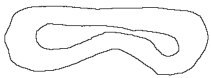
\includegraphics[interpolate=true,width=2.110000in,height=0.780000in]{contents/chapt7/figs/c_s/c_sr_lap_3-img0.png}}%
\end{pgfscope}%
\begin{pgfscope}%
\pgfpathrectangle{\pgfqpoint{0.892417in}{1.935046in}}{\pgfqpoint{2.108735in}{0.778610in}}%
\pgfusepath{clip}%
\pgfsetbuttcap%
\pgfsetroundjoin%
\pgfsetlinewidth{1.505625pt}%
\definecolor{currentstroke}{rgb}{1.000000,0.000000,0.000000}%
\pgfsetstrokecolor{currentstroke}%
\pgfsetdash{{1.500000pt}{2.475000pt}}{0.000000pt}%
\pgfpathmoveto{\pgfqpoint{2.048903in}{2.176698in}}%
\pgfpathlineto{\pgfqpoint{2.048903in}{2.436235in}}%
\pgfusepath{stroke}%
\end{pgfscope}%
\begin{pgfscope}%
\pgfpathrectangle{\pgfqpoint{0.892417in}{1.935046in}}{\pgfqpoint{2.108735in}{0.778610in}}%
\pgfusepath{clip}%
\pgfsetrectcap%
\pgfsetroundjoin%
\pgfsetlinewidth{1.505625pt}%
\definecolor{currentstroke}{rgb}{0.121569,0.466667,0.705882}%
\pgfsetstrokecolor{currentstroke}%
\pgfsetstrokeopacity{0.700000}%
\pgfsetdash{}{0pt}%
\pgfpathmoveto{\pgfqpoint{2.047355in}{2.285421in}}%
\pgfpathlineto{\pgfqpoint{2.087600in}{2.284397in}}%
\pgfpathlineto{\pgfqpoint{2.113002in}{2.281356in}}%
\pgfpathlineto{\pgfqpoint{2.139114in}{2.275816in}}%
\pgfpathlineto{\pgfqpoint{2.176461in}{2.264726in}}%
\pgfpathlineto{\pgfqpoint{2.245260in}{2.241493in}}%
\pgfpathlineto{\pgfqpoint{2.284174in}{2.226826in}}%
\pgfpathlineto{\pgfqpoint{2.317098in}{2.212114in}}%
\pgfpathlineto{\pgfqpoint{2.343894in}{2.197871in}}%
\pgfpathlineto{\pgfqpoint{2.375322in}{2.178279in}}%
\pgfpathlineto{\pgfqpoint{2.406260in}{2.156426in}}%
\pgfpathlineto{\pgfqpoint{2.441908in}{2.128663in}}%
\pgfpathlineto{\pgfqpoint{2.522962in}{2.063871in}}%
\pgfpathlineto{\pgfqpoint{2.545350in}{2.050766in}}%
\pgfpathlineto{\pgfqpoint{2.563048in}{2.042838in}}%
\pgfpathlineto{\pgfqpoint{2.581354in}{2.037074in}}%
\pgfpathlineto{\pgfqpoint{2.600066in}{2.033828in}}%
\pgfpathlineto{\pgfqpoint{2.618852in}{2.033415in}}%
\pgfpathlineto{\pgfqpoint{2.637261in}{2.036009in}}%
\pgfpathlineto{\pgfqpoint{2.654762in}{2.041662in}}%
\pgfpathlineto{\pgfqpoint{2.670803in}{2.050244in}}%
\pgfpathlineto{\pgfqpoint{2.685518in}{2.061973in}}%
\pgfpathlineto{\pgfqpoint{2.698905in}{2.076169in}}%
\pgfpathlineto{\pgfqpoint{2.710689in}{2.091728in}}%
\pgfpathlineto{\pgfqpoint{2.724342in}{2.113881in}}%
\pgfpathlineto{\pgfqpoint{2.736071in}{2.137113in}}%
\pgfpathlineto{\pgfqpoint{2.748460in}{2.167194in}}%
\pgfpathlineto{\pgfqpoint{2.756579in}{2.191922in}}%
\pgfpathlineto{\pgfqpoint{2.762793in}{2.217195in}}%
\pgfpathlineto{\pgfqpoint{2.766887in}{2.242894in}}%
\pgfpathlineto{\pgfqpoint{2.768543in}{2.268863in}}%
\pgfpathlineto{\pgfqpoint{2.767472in}{2.294861in}}%
\pgfpathlineto{\pgfqpoint{2.764568in}{2.314159in}}%
\pgfpathlineto{\pgfqpoint{2.759597in}{2.333031in}}%
\pgfpathlineto{\pgfqpoint{2.752496in}{2.351206in}}%
\pgfpathlineto{\pgfqpoint{2.743204in}{2.368363in}}%
\pgfpathlineto{\pgfqpoint{2.731750in}{2.384158in}}%
\pgfpathlineto{\pgfqpoint{2.718237in}{2.398231in}}%
\pgfpathlineto{\pgfqpoint{2.702911in}{2.410304in}}%
\pgfpathlineto{\pgfqpoint{2.686157in}{2.420306in}}%
\pgfpathlineto{\pgfqpoint{2.668357in}{2.428307in}}%
\pgfpathlineto{\pgfqpoint{2.649859in}{2.434538in}}%
\pgfpathlineto{\pgfqpoint{2.624533in}{2.440515in}}%
\pgfpathlineto{\pgfqpoint{2.598790in}{2.444345in}}%
\pgfpathlineto{\pgfqpoint{2.559873in}{2.447483in}}%
\pgfpathlineto{\pgfqpoint{2.507990in}{2.451710in}}%
\pgfpathlineto{\pgfqpoint{2.482294in}{2.455836in}}%
\pgfpathlineto{\pgfqpoint{2.457053in}{2.462165in}}%
\pgfpathlineto{\pgfqpoint{2.432495in}{2.470777in}}%
\pgfpathlineto{\pgfqpoint{2.402830in}{2.484128in}}%
\pgfpathlineto{\pgfqpoint{2.374145in}{2.499483in}}%
\pgfpathlineto{\pgfqpoint{2.318248in}{2.532808in}}%
\pgfpathlineto{\pgfqpoint{2.284003in}{2.551554in}}%
\pgfpathlineto{\pgfqpoint{2.254344in}{2.564917in}}%
\pgfpathlineto{\pgfqpoint{2.229781in}{2.573514in}}%
\pgfpathlineto{\pgfqpoint{2.204598in}{2.580082in}}%
\pgfpathlineto{\pgfqpoint{2.178959in}{2.584547in}}%
\pgfpathlineto{\pgfqpoint{2.153041in}{2.586905in}}%
\pgfpathlineto{\pgfqpoint{2.127017in}{2.587215in}}%
\pgfpathlineto{\pgfqpoint{2.101045in}{2.585539in}}%
\pgfpathlineto{\pgfqpoint{2.068806in}{2.581164in}}%
\pgfpathlineto{\pgfqpoint{1.966012in}{2.564715in}}%
\pgfpathlineto{\pgfqpoint{1.933560in}{2.562409in}}%
\pgfpathlineto{\pgfqpoint{1.901027in}{2.562295in}}%
\pgfpathlineto{\pgfqpoint{1.868567in}{2.564478in}}%
\pgfpathlineto{\pgfqpoint{1.836342in}{2.568948in}}%
\pgfpathlineto{\pgfqpoint{1.791705in}{2.578029in}}%
\pgfpathlineto{\pgfqpoint{1.721645in}{2.592707in}}%
\pgfpathlineto{\pgfqpoint{1.683011in}{2.598328in}}%
\pgfpathlineto{\pgfqpoint{1.650580in}{2.600931in}}%
\pgfpathlineto{\pgfqpoint{1.618050in}{2.601423in}}%
\pgfpathlineto{\pgfqpoint{1.585562in}{2.599699in}}%
\pgfpathlineto{\pgfqpoint{1.546790in}{2.595104in}}%
\pgfpathlineto{\pgfqpoint{1.476110in}{2.583756in}}%
\pgfpathlineto{\pgfqpoint{1.309230in}{2.555943in}}%
\pgfpathlineto{\pgfqpoint{1.277762in}{2.547698in}}%
\pgfpathlineto{\pgfqpoint{1.253269in}{2.538904in}}%
\pgfpathlineto{\pgfqpoint{1.229787in}{2.527698in}}%
\pgfpathlineto{\pgfqpoint{1.213132in}{2.517523in}}%
\pgfpathlineto{\pgfqpoint{1.197577in}{2.505737in}}%
\pgfpathlineto{\pgfqpoint{1.183385in}{2.492341in}}%
\pgfpathlineto{\pgfqpoint{1.170789in}{2.477437in}}%
\pgfpathlineto{\pgfqpoint{1.160023in}{2.461162in}}%
\pgfpathlineto{\pgfqpoint{1.151279in}{2.443718in}}%
\pgfpathlineto{\pgfqpoint{1.144732in}{2.425336in}}%
\pgfpathlineto{\pgfqpoint{1.140500in}{2.406288in}}%
\pgfpathlineto{\pgfqpoint{1.138535in}{2.386872in}}%
\pgfpathlineto{\pgfqpoint{1.138631in}{2.367356in}}%
\pgfpathlineto{\pgfqpoint{1.140669in}{2.347946in}}%
\pgfpathlineto{\pgfqpoint{1.144512in}{2.328810in}}%
\pgfpathlineto{\pgfqpoint{1.152145in}{2.303935in}}%
\pgfpathlineto{\pgfqpoint{1.162333in}{2.279991in}}%
\pgfpathlineto{\pgfqpoint{1.174737in}{2.257114in}}%
\pgfpathlineto{\pgfqpoint{1.189082in}{2.235400in}}%
\pgfpathlineto{\pgfqpoint{1.205163in}{2.214937in}}%
\pgfpathlineto{\pgfqpoint{1.222796in}{2.195795in}}%
\pgfpathlineto{\pgfqpoint{1.241792in}{2.178072in}}%
\pgfpathlineto{\pgfqpoint{1.261673in}{2.162304in}}%
\pgfpathlineto{\pgfqpoint{1.282331in}{2.148889in}}%
\pgfpathlineto{\pgfqpoint{1.303649in}{2.138112in}}%
\pgfpathlineto{\pgfqpoint{1.325420in}{2.130259in}}%
\pgfpathlineto{\pgfqpoint{1.341849in}{2.126406in}}%
\pgfpathlineto{\pgfqpoint{1.364441in}{2.123835in}}%
\pgfpathlineto{\pgfqpoint{1.387867in}{2.123589in}}%
\pgfpathlineto{\pgfqpoint{1.418039in}{2.125719in}}%
\pgfpathlineto{\pgfqpoint{1.455379in}{2.130970in}}%
\pgfpathlineto{\pgfqpoint{1.493584in}{2.138647in}}%
\pgfpathlineto{\pgfqpoint{1.537807in}{2.149783in}}%
\pgfpathlineto{\pgfqpoint{1.581433in}{2.163071in}}%
\pgfpathlineto{\pgfqpoint{1.630562in}{2.180476in}}%
\pgfpathlineto{\pgfqpoint{1.691115in}{2.204521in}}%
\pgfpathlineto{\pgfqpoint{1.823766in}{2.258804in}}%
\pgfpathlineto{\pgfqpoint{1.866923in}{2.273537in}}%
\pgfpathlineto{\pgfqpoint{1.904600in}{2.283942in}}%
\pgfpathlineto{\pgfqpoint{1.936474in}{2.290653in}}%
\pgfpathlineto{\pgfqpoint{1.968709in}{2.295323in}}%
\pgfpathlineto{\pgfqpoint{1.994702in}{2.297125in}}%
\pgfpathlineto{\pgfqpoint{2.020755in}{2.296806in}}%
\pgfpathlineto{\pgfqpoint{2.046668in}{2.294106in}}%
\pgfpathlineto{\pgfqpoint{2.046668in}{2.294106in}}%
\pgfusepath{stroke}%
\end{pgfscope}%
\begin{pgfscope}%
\pgfpathrectangle{\pgfqpoint{0.892417in}{1.935046in}}{\pgfqpoint{2.108735in}{0.778610in}}%
\pgfusepath{clip}%
\pgfsetrectcap%
\pgfsetroundjoin%
\pgfsetlinewidth{1.505625pt}%
\definecolor{currentstroke}{rgb}{1.000000,0.498039,0.054902}%
\pgfsetstrokecolor{currentstroke}%
\pgfsetstrokeopacity{0.700000}%
\pgfsetdash{}{0pt}%
\pgfpathmoveto{\pgfqpoint{2.047355in}{2.285421in}}%
\pgfpathlineto{\pgfqpoint{2.087645in}{2.284425in}}%
\pgfpathlineto{\pgfqpoint{2.113130in}{2.281464in}}%
\pgfpathlineto{\pgfqpoint{2.139361in}{2.275945in}}%
\pgfpathlineto{\pgfqpoint{2.172133in}{2.266097in}}%
\pgfpathlineto{\pgfqpoint{2.224349in}{2.247661in}}%
\pgfpathlineto{\pgfqpoint{2.281134in}{2.225673in}}%
\pgfpathlineto{\pgfqpoint{2.321188in}{2.208159in}}%
\pgfpathlineto{\pgfqpoint{2.361060in}{2.188186in}}%
\pgfpathlineto{\pgfqpoint{2.400498in}{2.165599in}}%
\pgfpathlineto{\pgfqpoint{2.433304in}{2.144478in}}%
\pgfpathlineto{\pgfqpoint{2.465048in}{2.121793in}}%
\pgfpathlineto{\pgfqpoint{2.543334in}{2.063662in}}%
\pgfpathlineto{\pgfqpoint{2.566124in}{2.051144in}}%
\pgfpathlineto{\pgfqpoint{2.584000in}{2.043757in}}%
\pgfpathlineto{\pgfqpoint{2.602412in}{2.038678in}}%
\pgfpathlineto{\pgfqpoint{2.621126in}{2.036372in}}%
\pgfpathlineto{\pgfqpoint{2.633569in}{2.036577in}}%
\pgfpathlineto{\pgfqpoint{2.645787in}{2.038288in}}%
\pgfpathlineto{\pgfqpoint{2.657572in}{2.041558in}}%
\pgfpathlineto{\pgfqpoint{2.668689in}{2.046394in}}%
\pgfpathlineto{\pgfqpoint{2.678890in}{2.052747in}}%
\pgfpathlineto{\pgfqpoint{2.688003in}{2.060612in}}%
\pgfpathlineto{\pgfqpoint{2.696068in}{2.070096in}}%
\pgfpathlineto{\pgfqpoint{2.703038in}{2.080903in}}%
\pgfpathlineto{\pgfqpoint{2.711432in}{2.098774in}}%
\pgfpathlineto{\pgfqpoint{2.717480in}{2.117575in}}%
\pgfpathlineto{\pgfqpoint{2.721621in}{2.136889in}}%
\pgfpathlineto{\pgfqpoint{2.724779in}{2.163036in}}%
\pgfpathlineto{\pgfqpoint{2.725795in}{2.189357in}}%
\pgfpathlineto{\pgfqpoint{2.724750in}{2.228856in}}%
\pgfpathlineto{\pgfqpoint{2.719023in}{2.353853in}}%
\pgfpathlineto{\pgfqpoint{2.716690in}{2.399890in}}%
\pgfpathlineto{\pgfqpoint{2.713132in}{2.425987in}}%
\pgfpathlineto{\pgfqpoint{2.708760in}{2.445193in}}%
\pgfpathlineto{\pgfqpoint{2.702548in}{2.463403in}}%
\pgfpathlineto{\pgfqpoint{2.694218in}{2.480179in}}%
\pgfpathlineto{\pgfqpoint{2.683604in}{2.494982in}}%
\pgfpathlineto{\pgfqpoint{2.675250in}{2.503413in}}%
\pgfpathlineto{\pgfqpoint{2.665961in}{2.510430in}}%
\pgfpathlineto{\pgfqpoint{2.655892in}{2.515807in}}%
\pgfpathlineto{\pgfqpoint{2.645278in}{2.519345in}}%
\pgfpathlineto{\pgfqpoint{2.634425in}{2.520890in}}%
\pgfpathlineto{\pgfqpoint{2.623271in}{2.520210in}}%
\pgfpathlineto{\pgfqpoint{2.612073in}{2.517412in}}%
\pgfpathlineto{\pgfqpoint{2.601087in}{2.512818in}}%
\pgfpathlineto{\pgfqpoint{2.585186in}{2.503287in}}%
\pgfpathlineto{\pgfqpoint{2.569878in}{2.491427in}}%
\pgfpathlineto{\pgfqpoint{2.550595in}{2.473711in}}%
\pgfpathlineto{\pgfqpoint{2.493082in}{2.418434in}}%
\pgfpathlineto{\pgfqpoint{2.476123in}{2.406467in}}%
\pgfpathlineto{\pgfqpoint{2.463414in}{2.399847in}}%
\pgfpathlineto{\pgfqpoint{2.450842in}{2.395617in}}%
\pgfpathlineto{\pgfqpoint{2.438255in}{2.394161in}}%
\pgfpathlineto{\pgfqpoint{2.425265in}{2.395646in}}%
\pgfpathlineto{\pgfqpoint{2.412320in}{2.399392in}}%
\pgfpathlineto{\pgfqpoint{2.395318in}{2.406878in}}%
\pgfpathlineto{\pgfqpoint{2.378614in}{2.416505in}}%
\pgfpathlineto{\pgfqpoint{2.358027in}{2.430907in}}%
\pgfpathlineto{\pgfqpoint{2.323438in}{2.458847in}}%
\pgfpathlineto{\pgfqpoint{2.278983in}{2.493997in}}%
\pgfpathlineto{\pgfqpoint{2.252356in}{2.512701in}}%
\pgfpathlineto{\pgfqpoint{2.230052in}{2.526120in}}%
\pgfpathlineto{\pgfqpoint{2.206710in}{2.537632in}}%
\pgfpathlineto{\pgfqpoint{2.182335in}{2.546747in}}%
\pgfpathlineto{\pgfqpoint{2.163458in}{2.551718in}}%
\pgfpathlineto{\pgfqpoint{2.144196in}{2.554878in}}%
\pgfpathlineto{\pgfqpoint{2.124718in}{2.556153in}}%
\pgfpathlineto{\pgfqpoint{2.098714in}{2.555153in}}%
\pgfpathlineto{\pgfqpoint{2.072934in}{2.551572in}}%
\pgfpathlineto{\pgfqpoint{2.041160in}{2.544566in}}%
\pgfpathlineto{\pgfqpoint{1.946515in}{2.520794in}}%
\pgfpathlineto{\pgfqpoint{1.920683in}{2.517606in}}%
\pgfpathlineto{\pgfqpoint{1.894667in}{2.516987in}}%
\pgfpathlineto{\pgfqpoint{1.875203in}{2.518472in}}%
\pgfpathlineto{\pgfqpoint{1.849568in}{2.522954in}}%
\pgfpathlineto{\pgfqpoint{1.824482in}{2.529894in}}%
\pgfpathlineto{\pgfqpoint{1.800025in}{2.538807in}}%
\pgfpathlineto{\pgfqpoint{1.770287in}{2.552014in}}%
\pgfpathlineto{\pgfqpoint{1.700094in}{2.585062in}}%
\pgfpathlineto{\pgfqpoint{1.676022in}{2.593928in}}%
\pgfpathlineto{\pgfqpoint{1.651374in}{2.600641in}}%
\pgfpathlineto{\pgfqpoint{1.625670in}{2.604821in}}%
\pgfpathlineto{\pgfqpoint{1.599604in}{2.606544in}}%
\pgfpathlineto{\pgfqpoint{1.573487in}{2.606015in}}%
\pgfpathlineto{\pgfqpoint{1.547498in}{2.603361in}}%
\pgfpathlineto{\pgfqpoint{1.515386in}{2.597433in}}%
\pgfpathlineto{\pgfqpoint{1.477472in}{2.587513in}}%
\pgfpathlineto{\pgfqpoint{1.415046in}{2.568275in}}%
\pgfpathlineto{\pgfqpoint{1.333591in}{2.544257in}}%
\pgfpathlineto{\pgfqpoint{1.283759in}{2.528528in}}%
\pgfpathlineto{\pgfqpoint{1.253187in}{2.517042in}}%
\pgfpathlineto{\pgfqpoint{1.229483in}{2.506063in}}%
\pgfpathlineto{\pgfqpoint{1.212486in}{2.496318in}}%
\pgfpathlineto{\pgfqpoint{1.196441in}{2.485078in}}%
\pgfpathlineto{\pgfqpoint{1.181657in}{2.472227in}}%
\pgfpathlineto{\pgfqpoint{1.168522in}{2.457699in}}%
\pgfpathlineto{\pgfqpoint{1.157431in}{2.441558in}}%
\pgfpathlineto{\pgfqpoint{1.148687in}{2.424036in}}%
\pgfpathlineto{\pgfqpoint{1.142575in}{2.405433in}}%
\pgfpathlineto{\pgfqpoint{1.139342in}{2.386121in}}%
\pgfpathlineto{\pgfqpoint{1.139112in}{2.366542in}}%
\pgfpathlineto{\pgfqpoint{1.141931in}{2.347166in}}%
\pgfpathlineto{\pgfqpoint{1.147741in}{2.328468in}}%
\pgfpathlineto{\pgfqpoint{1.156401in}{2.310907in}}%
\pgfpathlineto{\pgfqpoint{1.167539in}{2.294800in}}%
\pgfpathlineto{\pgfqpoint{1.180725in}{2.280318in}}%
\pgfpathlineto{\pgfqpoint{1.195511in}{2.267467in}}%
\pgfpathlineto{\pgfqpoint{1.216944in}{2.252540in}}%
\pgfpathlineto{\pgfqpoint{1.239595in}{2.239521in}}%
\pgfpathlineto{\pgfqpoint{1.318465in}{2.197206in}}%
\pgfpathlineto{\pgfqpoint{1.338846in}{2.182870in}}%
\pgfpathlineto{\pgfqpoint{1.357214in}{2.166824in}}%
\pgfpathlineto{\pgfqpoint{1.372660in}{2.149868in}}%
\pgfpathlineto{\pgfqpoint{1.385088in}{2.132440in}}%
\pgfpathlineto{\pgfqpoint{1.394580in}{2.114976in}}%
\pgfpathlineto{\pgfqpoint{1.403068in}{2.093928in}}%
\pgfpathlineto{\pgfqpoint{1.412111in}{2.063425in}}%
\pgfpathlineto{\pgfqpoint{1.420608in}{2.037603in}}%
\pgfpathlineto{\pgfqpoint{1.428906in}{2.020052in}}%
\pgfpathlineto{\pgfqpoint{1.434974in}{2.010103in}}%
\pgfpathlineto{\pgfqpoint{1.434974in}{2.010103in}}%
\pgfusepath{stroke}%
\end{pgfscope}%
\begin{pgfscope}%
\pgfsetbuttcap%
\pgfsetmiterjoin%
\definecolor{currentfill}{rgb}{1.000000,1.000000,1.000000}%
\pgfsetfillcolor{currentfill}%
\pgfsetlinewidth{1.003750pt}%
\definecolor{currentstroke}{rgb}{0.000000,0.000000,0.000000}%
\pgfsetstrokecolor{currentstroke}%
\pgfsetdash{}{0pt}%
\pgfpathmoveto{\pgfqpoint{2.760874in}{2.113140in}}%
\pgfpathlineto{\pgfqpoint{3.018023in}{2.113140in}}%
\pgfpathquadraticcurveto{\pgfqpoint{3.029593in}{2.113140in}}{\pgfqpoint{3.029593in}{2.124709in}}%
\pgfpathlineto{\pgfqpoint{3.029593in}{2.236675in}}%
\pgfpathquadraticcurveto{\pgfqpoint{3.029593in}{2.248245in}}{\pgfqpoint{3.018023in}{2.248245in}}%
\pgfpathlineto{\pgfqpoint{2.760874in}{2.248245in}}%
\pgfpathquadraticcurveto{\pgfqpoint{2.749305in}{2.248245in}}{\pgfqpoint{2.749305in}{2.236675in}}%
\pgfpathlineto{\pgfqpoint{2.749305in}{2.124709in}}%
\pgfpathquadraticcurveto{\pgfqpoint{2.749305in}{2.113140in}}{\pgfqpoint{2.760874in}{2.113140in}}%
\pgfpathlineto{\pgfqpoint{2.760874in}{2.113140in}}%
\pgfpathclose%
\pgfusepath{stroke,fill}%
\end{pgfscope}%
\begin{pgfscope}%
\definecolor{textcolor}{rgb}{0.000000,0.000000,0.000000}%
\pgfsetstrokecolor{textcolor}%
\pgfsetfillcolor{textcolor}%
\pgftext[x=2.760874in,y=2.148775in,left,base]{\color{textcolor}\rmfamily\fontsize{8.330000}{9.996000}\selectfont 20\%}%
\end{pgfscope}%
\begin{pgfscope}%
\pgfsetbuttcap%
\pgfsetmiterjoin%
\definecolor{currentfill}{rgb}{1.000000,1.000000,1.000000}%
\pgfsetfillcolor{currentfill}%
\pgfsetlinewidth{1.003750pt}%
\definecolor{currentstroke}{rgb}{0.000000,0.000000,0.000000}%
\pgfsetstrokecolor{currentstroke}%
\pgfsetdash{}{0pt}%
\pgfpathmoveto{\pgfqpoint{2.289177in}{2.485413in}}%
\pgfpathlineto{\pgfqpoint{2.546325in}{2.485413in}}%
\pgfpathquadraticcurveto{\pgfqpoint{2.557895in}{2.485413in}}{\pgfqpoint{2.557895in}{2.496983in}}%
\pgfpathlineto{\pgfqpoint{2.557895in}{2.608948in}}%
\pgfpathquadraticcurveto{\pgfqpoint{2.557895in}{2.620518in}}{\pgfqpoint{2.546325in}{2.620518in}}%
\pgfpathlineto{\pgfqpoint{2.289177in}{2.620518in}}%
\pgfpathquadraticcurveto{\pgfqpoint{2.277607in}{2.620518in}}{\pgfqpoint{2.277607in}{2.608948in}}%
\pgfpathlineto{\pgfqpoint{2.277607in}{2.496983in}}%
\pgfpathquadraticcurveto{\pgfqpoint{2.277607in}{2.485413in}}{\pgfqpoint{2.289177in}{2.485413in}}%
\pgfpathlineto{\pgfqpoint{2.289177in}{2.485413in}}%
\pgfpathclose%
\pgfusepath{stroke,fill}%
\end{pgfscope}%
\begin{pgfscope}%
\definecolor{textcolor}{rgb}{0.000000,0.000000,0.000000}%
\pgfsetstrokecolor{textcolor}%
\pgfsetfillcolor{textcolor}%
\pgftext[x=2.289177in,y=2.521048in,left,base]{\color{textcolor}\rmfamily\fontsize{8.330000}{9.996000}\selectfont 40\%}%
\end{pgfscope}%
\begin{pgfscope}%
\pgfsetbuttcap%
\pgfsetmiterjoin%
\definecolor{currentfill}{rgb}{1.000000,1.000000,1.000000}%
\pgfsetfillcolor{currentfill}%
\pgfsetlinewidth{1.003750pt}%
\definecolor{currentstroke}{rgb}{0.000000,0.000000,0.000000}%
\pgfsetstrokecolor{currentstroke}%
\pgfsetdash{}{0pt}%
\pgfpathmoveto{\pgfqpoint{1.486615in}{2.524361in}}%
\pgfpathlineto{\pgfqpoint{1.743764in}{2.524361in}}%
\pgfpathquadraticcurveto{\pgfqpoint{1.755333in}{2.524361in}}{\pgfqpoint{1.755333in}{2.535931in}}%
\pgfpathlineto{\pgfqpoint{1.755333in}{2.647897in}}%
\pgfpathquadraticcurveto{\pgfqpoint{1.755333in}{2.659466in}}{\pgfqpoint{1.743764in}{2.659466in}}%
\pgfpathlineto{\pgfqpoint{1.486615in}{2.659466in}}%
\pgfpathquadraticcurveto{\pgfqpoint{1.475046in}{2.659466in}}{\pgfqpoint{1.475046in}{2.647897in}}%
\pgfpathlineto{\pgfqpoint{1.475046in}{2.535931in}}%
\pgfpathquadraticcurveto{\pgfqpoint{1.475046in}{2.524361in}}{\pgfqpoint{1.486615in}{2.524361in}}%
\pgfpathlineto{\pgfqpoint{1.486615in}{2.524361in}}%
\pgfpathclose%
\pgfusepath{stroke,fill}%
\end{pgfscope}%
\begin{pgfscope}%
\definecolor{textcolor}{rgb}{0.000000,0.000000,0.000000}%
\pgfsetstrokecolor{textcolor}%
\pgfsetfillcolor{textcolor}%
\pgftext[x=1.486615in,y=2.559996in,left,base]{\color{textcolor}\rmfamily\fontsize{8.330000}{9.996000}\selectfont 60\%}%
\end{pgfscope}%
\begin{pgfscope}%
\pgfsetbuttcap%
\pgfsetmiterjoin%
\definecolor{currentfill}{rgb}{1.000000,1.000000,1.000000}%
\pgfsetfillcolor{currentfill}%
\pgfsetlinewidth{1.003750pt}%
\definecolor{currentstroke}{rgb}{0.000000,0.000000,0.000000}%
\pgfsetstrokecolor{currentstroke}%
\pgfsetdash{}{0pt}%
\pgfpathmoveto{\pgfqpoint{1.275724in}{2.092218in}}%
\pgfpathlineto{\pgfqpoint{1.532873in}{2.092218in}}%
\pgfpathquadraticcurveto{\pgfqpoint{1.544442in}{2.092218in}}{\pgfqpoint{1.544442in}{2.103788in}}%
\pgfpathlineto{\pgfqpoint{1.544442in}{2.215754in}}%
\pgfpathquadraticcurveto{\pgfqpoint{1.544442in}{2.227323in}}{\pgfqpoint{1.532873in}{2.227323in}}%
\pgfpathlineto{\pgfqpoint{1.275724in}{2.227323in}}%
\pgfpathquadraticcurveto{\pgfqpoint{1.264154in}{2.227323in}}{\pgfqpoint{1.264154in}{2.215754in}}%
\pgfpathlineto{\pgfqpoint{1.264154in}{2.103788in}}%
\pgfpathquadraticcurveto{\pgfqpoint{1.264154in}{2.092218in}}{\pgfqpoint{1.275724in}{2.092218in}}%
\pgfpathlineto{\pgfqpoint{1.275724in}{2.092218in}}%
\pgfpathclose%
\pgfusepath{stroke,fill}%
\end{pgfscope}%
\begin{pgfscope}%
\definecolor{textcolor}{rgb}{0.000000,0.000000,0.000000}%
\pgfsetstrokecolor{textcolor}%
\pgfsetfillcolor{textcolor}%
\pgftext[x=1.275724in,y=2.127853in,left,base]{\color{textcolor}\rmfamily\fontsize{8.330000}{9.996000}\selectfont 80\%}%
\end{pgfscope}%
\begin{pgfscope}%
\definecolor{textcolor}{rgb}{0.000000,0.000000,0.000000}%
\pgfsetstrokecolor{textcolor}%
\pgfsetfillcolor{textcolor}%
\pgftext[x=1.946784in,y=2.796989in,,base]{\color{textcolor}\rmfamily\fontsize{12.000000}{14.400000}\selectfont End-to-end}%
\end{pgfscope}%
\begin{pgfscope}%
\pgfpathrectangle{\pgfqpoint{3.196208in}{1.935046in}}{\pgfqpoint{2.108735in}{0.778610in}}%
\pgfusepath{clip}%
\pgfsys@transformshift{3.196208in}{1.935046in}%
\pgftext[left,bottom]{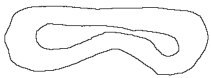
\includegraphics[interpolate=true,width=2.110000in,height=0.780000in]{contents/chapt7/figs/c_s/c_sr_lap_3-img1.png}}%
\end{pgfscope}%
\begin{pgfscope}%
\pgfpathrectangle{\pgfqpoint{3.196208in}{1.935046in}}{\pgfqpoint{2.108735in}{0.778610in}}%
\pgfusepath{clip}%
\pgfsetbuttcap%
\pgfsetroundjoin%
\pgfsetlinewidth{1.505625pt}%
\definecolor{currentstroke}{rgb}{1.000000,0.000000,0.000000}%
\pgfsetstrokecolor{currentstroke}%
\pgfsetdash{{1.500000pt}{2.475000pt}}{0.000000pt}%
\pgfpathmoveto{\pgfqpoint{4.352694in}{2.176698in}}%
\pgfpathlineto{\pgfqpoint{4.352694in}{2.436235in}}%
\pgfusepath{stroke}%
\end{pgfscope}%
\begin{pgfscope}%
\pgfpathrectangle{\pgfqpoint{3.196208in}{1.935046in}}{\pgfqpoint{2.108735in}{0.778610in}}%
\pgfusepath{clip}%
\pgfsetrectcap%
\pgfsetroundjoin%
\pgfsetlinewidth{1.505625pt}%
\definecolor{currentstroke}{rgb}{0.121569,0.466667,0.705882}%
\pgfsetstrokecolor{currentstroke}%
\pgfsetstrokeopacity{0.700000}%
\pgfsetdash{}{0pt}%
\pgfpathmoveto{\pgfqpoint{4.351146in}{2.285421in}}%
\pgfpathlineto{\pgfqpoint{4.400584in}{2.284315in}}%
\pgfpathlineto{\pgfqpoint{4.432579in}{2.281152in}}%
\pgfpathlineto{\pgfqpoint{4.460616in}{2.276382in}}%
\pgfpathlineto{\pgfqpoint{4.489225in}{2.269401in}}%
\pgfpathlineto{\pgfqpoint{4.517989in}{2.260006in}}%
\pgfpathlineto{\pgfqpoint{4.546555in}{2.248085in}}%
\pgfpathlineto{\pgfqpoint{4.574355in}{2.233664in}}%
\pgfpathlineto{\pgfqpoint{4.606789in}{2.213684in}}%
\pgfpathlineto{\pgfqpoint{4.682373in}{2.165328in}}%
\pgfpathlineto{\pgfqpoint{4.716450in}{2.146788in}}%
\pgfpathlineto{\pgfqpoint{4.745888in}{2.133334in}}%
\pgfpathlineto{\pgfqpoint{4.776287in}{2.122250in}}%
\pgfpathlineto{\pgfqpoint{4.801209in}{2.115367in}}%
\pgfpathlineto{\pgfqpoint{4.826559in}{2.110494in}}%
\pgfpathlineto{\pgfqpoint{4.852309in}{2.107876in}}%
\pgfpathlineto{\pgfqpoint{4.878197in}{2.107642in}}%
\pgfpathlineto{\pgfqpoint{4.904048in}{2.109912in}}%
\pgfpathlineto{\pgfqpoint{4.929525in}{2.114843in}}%
\pgfpathlineto{\pgfqpoint{4.954330in}{2.122423in}}%
\pgfpathlineto{\pgfqpoint{4.978097in}{2.132688in}}%
\pgfpathlineto{\pgfqpoint{4.995059in}{2.142127in}}%
\pgfpathlineto{\pgfqpoint{5.011120in}{2.153014in}}%
\pgfpathlineto{\pgfqpoint{5.026152in}{2.165367in}}%
\pgfpathlineto{\pgfqpoint{5.039961in}{2.179042in}}%
\pgfpathlineto{\pgfqpoint{5.052238in}{2.193769in}}%
\pgfpathlineto{\pgfqpoint{5.062804in}{2.209412in}}%
\pgfpathlineto{\pgfqpoint{5.071486in}{2.225901in}}%
\pgfpathlineto{\pgfqpoint{5.078138in}{2.243076in}}%
\pgfpathlineto{\pgfqpoint{5.082653in}{2.260763in}}%
\pgfpathlineto{\pgfqpoint{5.084997in}{2.278701in}}%
\pgfpathlineto{\pgfqpoint{5.085168in}{2.296641in}}%
\pgfpathlineto{\pgfqpoint{5.083225in}{2.314390in}}%
\pgfpathlineto{\pgfqpoint{5.079242in}{2.331762in}}%
\pgfpathlineto{\pgfqpoint{5.073365in}{2.348540in}}%
\pgfpathlineto{\pgfqpoint{5.065747in}{2.364531in}}%
\pgfpathlineto{\pgfqpoint{5.056574in}{2.379622in}}%
\pgfpathlineto{\pgfqpoint{5.045981in}{2.393708in}}%
\pgfpathlineto{\pgfqpoint{5.029639in}{2.411111in}}%
\pgfpathlineto{\pgfqpoint{5.011175in}{2.426969in}}%
\pgfpathlineto{\pgfqpoint{4.991042in}{2.441164in}}%
\pgfpathlineto{\pgfqpoint{4.969448in}{2.453669in}}%
\pgfpathlineto{\pgfqpoint{4.946615in}{2.464386in}}%
\pgfpathlineto{\pgfqpoint{4.922769in}{2.473355in}}%
\pgfpathlineto{\pgfqpoint{4.885855in}{2.484429in}}%
\pgfpathlineto{\pgfqpoint{4.711059in}{2.531301in}}%
\pgfpathlineto{\pgfqpoint{4.678950in}{2.536078in}}%
\pgfpathlineto{\pgfqpoint{4.633667in}{2.540008in}}%
\pgfpathlineto{\pgfqpoint{4.556070in}{2.546438in}}%
\pgfpathlineto{\pgfqpoint{4.472194in}{2.555223in}}%
\pgfpathlineto{\pgfqpoint{4.439761in}{2.556145in}}%
\pgfpathlineto{\pgfqpoint{4.407344in}{2.554900in}}%
\pgfpathlineto{\pgfqpoint{4.362149in}{2.550801in}}%
\pgfpathlineto{\pgfqpoint{4.207308in}{2.534532in}}%
\pgfpathlineto{\pgfqpoint{4.155560in}{2.532322in}}%
\pgfpathlineto{\pgfqpoint{3.999910in}{2.527019in}}%
\pgfpathlineto{\pgfqpoint{3.792443in}{2.516129in}}%
\pgfpathlineto{\pgfqpoint{3.734255in}{2.510995in}}%
\pgfpathlineto{\pgfqpoint{3.689235in}{2.504961in}}%
\pgfpathlineto{\pgfqpoint{3.651040in}{2.497627in}}%
\pgfpathlineto{\pgfqpoint{3.619755in}{2.489446in}}%
\pgfpathlineto{\pgfqpoint{3.589166in}{2.478838in}}%
\pgfpathlineto{\pgfqpoint{3.565517in}{2.468218in}}%
\pgfpathlineto{\pgfqpoint{3.542960in}{2.455506in}}%
\pgfpathlineto{\pgfqpoint{3.522044in}{2.440597in}}%
\pgfpathlineto{\pgfqpoint{3.507737in}{2.427978in}}%
\pgfpathlineto{\pgfqpoint{3.494809in}{2.414144in}}%
\pgfpathlineto{\pgfqpoint{3.483460in}{2.399170in}}%
\pgfpathlineto{\pgfqpoint{3.473921in}{2.383159in}}%
\pgfpathlineto{\pgfqpoint{3.466329in}{2.366268in}}%
\pgfpathlineto{\pgfqpoint{3.460810in}{2.348678in}}%
\pgfpathlineto{\pgfqpoint{3.457435in}{2.330628in}}%
\pgfpathlineto{\pgfqpoint{3.456249in}{2.312361in}}%
\pgfpathlineto{\pgfqpoint{3.457234in}{2.294145in}}%
\pgfpathlineto{\pgfqpoint{3.460362in}{2.276232in}}%
\pgfpathlineto{\pgfqpoint{3.465514in}{2.258852in}}%
\pgfpathlineto{\pgfqpoint{3.472560in}{2.242199in}}%
\pgfpathlineto{\pgfqpoint{3.481480in}{2.226285in}}%
\pgfpathlineto{\pgfqpoint{3.492120in}{2.211189in}}%
\pgfpathlineto{\pgfqpoint{3.504265in}{2.197067in}}%
\pgfpathlineto{\pgfqpoint{3.517783in}{2.183958in}}%
\pgfpathlineto{\pgfqpoint{3.537638in}{2.168307in}}%
\pgfpathlineto{\pgfqpoint{3.559164in}{2.154940in}}%
\pgfpathlineto{\pgfqpoint{3.582143in}{2.143912in}}%
\pgfpathlineto{\pgfqpoint{3.606280in}{2.135167in}}%
\pgfpathlineto{\pgfqpoint{3.631276in}{2.128698in}}%
\pgfpathlineto{\pgfqpoint{3.656754in}{2.124478in}}%
\pgfpathlineto{\pgfqpoint{3.682490in}{2.122501in}}%
\pgfpathlineto{\pgfqpoint{3.708348in}{2.122652in}}%
\pgfpathlineto{\pgfqpoint{3.734144in}{2.124717in}}%
\pgfpathlineto{\pgfqpoint{3.766140in}{2.129810in}}%
\pgfpathlineto{\pgfqpoint{3.797675in}{2.137439in}}%
\pgfpathlineto{\pgfqpoint{3.828587in}{2.147321in}}%
\pgfpathlineto{\pgfqpoint{3.944931in}{2.188136in}}%
\pgfpathlineto{\pgfqpoint{3.988959in}{2.199254in}}%
\pgfpathlineto{\pgfqpoint{4.039849in}{2.209391in}}%
\pgfpathlineto{\pgfqpoint{4.110266in}{2.220801in}}%
\pgfpathlineto{\pgfqpoint{4.193805in}{2.232104in}}%
\pgfpathlineto{\pgfqpoint{4.251936in}{2.237894in}}%
\pgfpathlineto{\pgfqpoint{4.297310in}{2.240131in}}%
\pgfpathlineto{\pgfqpoint{4.310305in}{2.240307in}}%
\pgfpathlineto{\pgfqpoint{4.310305in}{2.240307in}}%
\pgfusepath{stroke}%
\end{pgfscope}%
\begin{pgfscope}%
\pgfpathrectangle{\pgfqpoint{3.196208in}{1.935046in}}{\pgfqpoint{2.108735in}{0.778610in}}%
\pgfusepath{clip}%
\pgfsetrectcap%
\pgfsetroundjoin%
\pgfsetlinewidth{1.505625pt}%
\definecolor{currentstroke}{rgb}{1.000000,0.498039,0.054902}%
\pgfsetstrokecolor{currentstroke}%
\pgfsetstrokeopacity{0.700000}%
\pgfsetdash{}{0pt}%
\pgfpathmoveto{\pgfqpoint{4.351146in}{2.285421in}}%
\pgfpathlineto{\pgfqpoint{4.400535in}{2.284336in}}%
\pgfpathlineto{\pgfqpoint{4.432356in}{2.281240in}}%
\pgfpathlineto{\pgfqpoint{4.460300in}{2.276485in}}%
\pgfpathlineto{\pgfqpoint{4.489026in}{2.269498in}}%
\pgfpathlineto{\pgfqpoint{4.518010in}{2.260160in}}%
\pgfpathlineto{\pgfqpoint{4.546674in}{2.248395in}}%
\pgfpathlineto{\pgfqpoint{4.574567in}{2.234151in}}%
\pgfpathlineto{\pgfqpoint{4.601593in}{2.217685in}}%
\pgfpathlineto{\pgfqpoint{4.649219in}{2.185298in}}%
\pgfpathlineto{\pgfqpoint{4.692361in}{2.157028in}}%
\pgfpathlineto{\pgfqpoint{4.720401in}{2.140942in}}%
\pgfpathlineto{\pgfqpoint{4.749493in}{2.126976in}}%
\pgfpathlineto{\pgfqpoint{4.773649in}{2.117733in}}%
\pgfpathlineto{\pgfqpoint{4.798457in}{2.110526in}}%
\pgfpathlineto{\pgfqpoint{4.823773in}{2.105631in}}%
\pgfpathlineto{\pgfqpoint{4.849522in}{2.103275in}}%
\pgfpathlineto{\pgfqpoint{4.875428in}{2.103618in}}%
\pgfpathlineto{\pgfqpoint{4.901227in}{2.106751in}}%
\pgfpathlineto{\pgfqpoint{4.926492in}{2.112685in}}%
\pgfpathlineto{\pgfqpoint{4.944902in}{2.118974in}}%
\pgfpathlineto{\pgfqpoint{4.962669in}{2.126863in}}%
\pgfpathlineto{\pgfqpoint{4.979655in}{2.136367in}}%
\pgfpathlineto{\pgfqpoint{4.995652in}{2.147393in}}%
\pgfpathlineto{\pgfqpoint{5.010503in}{2.159902in}}%
\pgfpathlineto{\pgfqpoint{5.024049in}{2.173802in}}%
\pgfpathlineto{\pgfqpoint{5.036075in}{2.188932in}}%
\pgfpathlineto{\pgfqpoint{5.046326in}{2.204987in}}%
\pgfpathlineto{\pgfqpoint{5.054642in}{2.221844in}}%
\pgfpathlineto{\pgfqpoint{5.060873in}{2.239342in}}%
\pgfpathlineto{\pgfqpoint{5.064867in}{2.257260in}}%
\pgfpathlineto{\pgfqpoint{5.066550in}{2.275358in}}%
\pgfpathlineto{\pgfqpoint{5.065881in}{2.293339in}}%
\pgfpathlineto{\pgfqpoint{5.062839in}{2.311197in}}%
\pgfpathlineto{\pgfqpoint{5.057514in}{2.328759in}}%
\pgfpathlineto{\pgfqpoint{5.050135in}{2.345793in}}%
\pgfpathlineto{\pgfqpoint{5.040954in}{2.362089in}}%
\pgfpathlineto{\pgfqpoint{5.030209in}{2.377545in}}%
\pgfpathlineto{\pgfqpoint{5.018049in}{2.392069in}}%
\pgfpathlineto{\pgfqpoint{4.999919in}{2.409775in}}%
\pgfpathlineto{\pgfqpoint{4.979856in}{2.425415in}}%
\pgfpathlineto{\pgfqpoint{4.958139in}{2.438836in}}%
\pgfpathlineto{\pgfqpoint{4.935084in}{2.449987in}}%
\pgfpathlineto{\pgfqpoint{4.911010in}{2.458861in}}%
\pgfpathlineto{\pgfqpoint{4.886156in}{2.465527in}}%
\pgfpathlineto{\pgfqpoint{4.854398in}{2.471578in}}%
\pgfpathlineto{\pgfqpoint{4.752171in}{2.489005in}}%
\pgfpathlineto{\pgfqpoint{4.714537in}{2.498804in}}%
\pgfpathlineto{\pgfqpoint{4.677419in}{2.510642in}}%
\pgfpathlineto{\pgfqpoint{4.573108in}{2.546183in}}%
\pgfpathlineto{\pgfqpoint{4.547786in}{2.551850in}}%
\pgfpathlineto{\pgfqpoint{4.522145in}{2.555454in}}%
\pgfpathlineto{\pgfqpoint{4.496326in}{2.556889in}}%
\pgfpathlineto{\pgfqpoint{4.463984in}{2.556191in}}%
\pgfpathlineto{\pgfqpoint{4.418681in}{2.552376in}}%
\pgfpathlineto{\pgfqpoint{4.328176in}{2.544071in}}%
\pgfpathlineto{\pgfqpoint{4.276137in}{2.541892in}}%
\pgfpathlineto{\pgfqpoint{4.126844in}{2.538264in}}%
\pgfpathlineto{\pgfqpoint{4.062261in}{2.532041in}}%
\pgfpathlineto{\pgfqpoint{3.984742in}{2.524926in}}%
\pgfpathlineto{\pgfqpoint{3.919953in}{2.521513in}}%
\pgfpathlineto{\pgfqpoint{3.771030in}{2.515061in}}%
\pgfpathlineto{\pgfqpoint{3.726007in}{2.510526in}}%
\pgfpathlineto{\pgfqpoint{3.681215in}{2.503773in}}%
\pgfpathlineto{\pgfqpoint{3.643154in}{2.495626in}}%
\pgfpathlineto{\pgfqpoint{3.612026in}{2.486663in}}%
\pgfpathlineto{\pgfqpoint{3.587686in}{2.477657in}}%
\pgfpathlineto{\pgfqpoint{3.564163in}{2.466695in}}%
\pgfpathlineto{\pgfqpoint{3.541830in}{2.453485in}}%
\pgfpathlineto{\pgfqpoint{3.526101in}{2.442009in}}%
\pgfpathlineto{\pgfqpoint{3.511490in}{2.429163in}}%
\pgfpathlineto{\pgfqpoint{3.498297in}{2.414962in}}%
\pgfpathlineto{\pgfqpoint{3.486815in}{2.399552in}}%
\pgfpathlineto{\pgfqpoint{3.477283in}{2.383032in}}%
\pgfpathlineto{\pgfqpoint{3.469886in}{2.365612in}}%
\pgfpathlineto{\pgfqpoint{3.464833in}{2.347492in}}%
\pgfpathlineto{\pgfqpoint{3.462257in}{2.328981in}}%
\pgfpathlineto{\pgfqpoint{3.462238in}{2.310459in}}%
\pgfpathlineto{\pgfqpoint{3.464814in}{2.292011in}}%
\pgfpathlineto{\pgfqpoint{3.469860in}{2.273868in}}%
\pgfpathlineto{\pgfqpoint{3.477151in}{2.256382in}}%
\pgfpathlineto{\pgfqpoint{3.486449in}{2.239782in}}%
\pgfpathlineto{\pgfqpoint{3.497559in}{2.224248in}}%
\pgfpathlineto{\pgfqpoint{3.510252in}{2.209957in}}%
\pgfpathlineto{\pgfqpoint{3.524378in}{2.197025in}}%
\pgfpathlineto{\pgfqpoint{3.539784in}{2.185487in}}%
\pgfpathlineto{\pgfqpoint{3.556285in}{2.175440in}}%
\pgfpathlineto{\pgfqpoint{3.573710in}{2.166927in}}%
\pgfpathlineto{\pgfqpoint{3.598002in}{2.157962in}}%
\pgfpathlineto{\pgfqpoint{3.623170in}{2.151762in}}%
\pgfpathlineto{\pgfqpoint{3.648869in}{2.148183in}}%
\pgfpathlineto{\pgfqpoint{3.674789in}{2.147030in}}%
\pgfpathlineto{\pgfqpoint{3.700659in}{2.148152in}}%
\pgfpathlineto{\pgfqpoint{3.726329in}{2.151334in}}%
\pgfpathlineto{\pgfqpoint{3.757971in}{2.157790in}}%
\pgfpathlineto{\pgfqpoint{3.789180in}{2.166571in}}%
\pgfpathlineto{\pgfqpoint{3.882409in}{2.194468in}}%
\pgfpathlineto{\pgfqpoint{3.920558in}{2.202373in}}%
\pgfpathlineto{\pgfqpoint{3.959128in}{2.208010in}}%
\pgfpathlineto{\pgfqpoint{4.010824in}{2.212820in}}%
\pgfpathlineto{\pgfqpoint{4.133722in}{2.223167in}}%
\pgfpathlineto{\pgfqpoint{4.217367in}{2.234053in}}%
\pgfpathlineto{\pgfqpoint{4.275342in}{2.240357in}}%
\pgfpathlineto{\pgfqpoint{4.314188in}{2.242234in}}%
\pgfpathlineto{\pgfqpoint{4.353170in}{2.241513in}}%
\pgfpathlineto{\pgfqpoint{4.353170in}{2.241513in}}%
\pgfusepath{stroke}%
\end{pgfscope}%
\begin{pgfscope}%
\pgfsetbuttcap%
\pgfsetmiterjoin%
\definecolor{currentfill}{rgb}{1.000000,1.000000,1.000000}%
\pgfsetfillcolor{currentfill}%
\pgfsetlinewidth{1.003750pt}%
\definecolor{currentstroke}{rgb}{0.000000,0.000000,0.000000}%
\pgfsetstrokecolor{currentstroke}%
\pgfsetdash{}{0pt}%
\pgfpathmoveto{\pgfqpoint{5.064666in}{2.113140in}}%
\pgfpathlineto{\pgfqpoint{5.321815in}{2.113140in}}%
\pgfpathquadraticcurveto{\pgfqpoint{5.333384in}{2.113140in}}{\pgfqpoint{5.333384in}{2.124709in}}%
\pgfpathlineto{\pgfqpoint{5.333384in}{2.236675in}}%
\pgfpathquadraticcurveto{\pgfqpoint{5.333384in}{2.248245in}}{\pgfqpoint{5.321815in}{2.248245in}}%
\pgfpathlineto{\pgfqpoint{5.064666in}{2.248245in}}%
\pgfpathquadraticcurveto{\pgfqpoint{5.053097in}{2.248245in}}{\pgfqpoint{5.053097in}{2.236675in}}%
\pgfpathlineto{\pgfqpoint{5.053097in}{2.124709in}}%
\pgfpathquadraticcurveto{\pgfqpoint{5.053097in}{2.113140in}}{\pgfqpoint{5.064666in}{2.113140in}}%
\pgfpathlineto{\pgfqpoint{5.064666in}{2.113140in}}%
\pgfpathclose%
\pgfusepath{stroke,fill}%
\end{pgfscope}%
\begin{pgfscope}%
\definecolor{textcolor}{rgb}{0.000000,0.000000,0.000000}%
\pgfsetstrokecolor{textcolor}%
\pgfsetfillcolor{textcolor}%
\pgftext[x=5.064666in,y=2.148775in,left,base]{\color{textcolor}\rmfamily\fontsize{8.330000}{9.996000}\selectfont 20\%}%
\end{pgfscope}%
\begin{pgfscope}%
\pgfsetbuttcap%
\pgfsetmiterjoin%
\definecolor{currentfill}{rgb}{1.000000,1.000000,1.000000}%
\pgfsetfillcolor{currentfill}%
\pgfsetlinewidth{1.003750pt}%
\definecolor{currentstroke}{rgb}{0.000000,0.000000,0.000000}%
\pgfsetstrokecolor{currentstroke}%
\pgfsetdash{}{0pt}%
\pgfpathmoveto{\pgfqpoint{4.592968in}{2.485413in}}%
\pgfpathlineto{\pgfqpoint{4.850117in}{2.485413in}}%
\pgfpathquadraticcurveto{\pgfqpoint{4.861687in}{2.485413in}}{\pgfqpoint{4.861687in}{2.496983in}}%
\pgfpathlineto{\pgfqpoint{4.861687in}{2.608948in}}%
\pgfpathquadraticcurveto{\pgfqpoint{4.861687in}{2.620518in}}{\pgfqpoint{4.850117in}{2.620518in}}%
\pgfpathlineto{\pgfqpoint{4.592968in}{2.620518in}}%
\pgfpathquadraticcurveto{\pgfqpoint{4.581399in}{2.620518in}}{\pgfqpoint{4.581399in}{2.608948in}}%
\pgfpathlineto{\pgfqpoint{4.581399in}{2.496983in}}%
\pgfpathquadraticcurveto{\pgfqpoint{4.581399in}{2.485413in}}{\pgfqpoint{4.592968in}{2.485413in}}%
\pgfpathlineto{\pgfqpoint{4.592968in}{2.485413in}}%
\pgfpathclose%
\pgfusepath{stroke,fill}%
\end{pgfscope}%
\begin{pgfscope}%
\definecolor{textcolor}{rgb}{0.000000,0.000000,0.000000}%
\pgfsetstrokecolor{textcolor}%
\pgfsetfillcolor{textcolor}%
\pgftext[x=4.592968in,y=2.521048in,left,base]{\color{textcolor}\rmfamily\fontsize{8.330000}{9.996000}\selectfont 40\%}%
\end{pgfscope}%
\begin{pgfscope}%
\pgfsetbuttcap%
\pgfsetmiterjoin%
\definecolor{currentfill}{rgb}{1.000000,1.000000,1.000000}%
\pgfsetfillcolor{currentfill}%
\pgfsetlinewidth{1.003750pt}%
\definecolor{currentstroke}{rgb}{0.000000,0.000000,0.000000}%
\pgfsetstrokecolor{currentstroke}%
\pgfsetdash{}{0pt}%
\pgfpathmoveto{\pgfqpoint{3.790407in}{2.524361in}}%
\pgfpathlineto{\pgfqpoint{4.047556in}{2.524361in}}%
\pgfpathquadraticcurveto{\pgfqpoint{4.059125in}{2.524361in}}{\pgfqpoint{4.059125in}{2.535931in}}%
\pgfpathlineto{\pgfqpoint{4.059125in}{2.647897in}}%
\pgfpathquadraticcurveto{\pgfqpoint{4.059125in}{2.659466in}}{\pgfqpoint{4.047556in}{2.659466in}}%
\pgfpathlineto{\pgfqpoint{3.790407in}{2.659466in}}%
\pgfpathquadraticcurveto{\pgfqpoint{3.778837in}{2.659466in}}{\pgfqpoint{3.778837in}{2.647897in}}%
\pgfpathlineto{\pgfqpoint{3.778837in}{2.535931in}}%
\pgfpathquadraticcurveto{\pgfqpoint{3.778837in}{2.524361in}}{\pgfqpoint{3.790407in}{2.524361in}}%
\pgfpathlineto{\pgfqpoint{3.790407in}{2.524361in}}%
\pgfpathclose%
\pgfusepath{stroke,fill}%
\end{pgfscope}%
\begin{pgfscope}%
\definecolor{textcolor}{rgb}{0.000000,0.000000,0.000000}%
\pgfsetstrokecolor{textcolor}%
\pgfsetfillcolor{textcolor}%
\pgftext[x=3.790407in,y=2.559996in,left,base]{\color{textcolor}\rmfamily\fontsize{8.330000}{9.996000}\selectfont 60\%}%
\end{pgfscope}%
\begin{pgfscope}%
\pgfsetbuttcap%
\pgfsetmiterjoin%
\definecolor{currentfill}{rgb}{1.000000,1.000000,1.000000}%
\pgfsetfillcolor{currentfill}%
\pgfsetlinewidth{1.003750pt}%
\definecolor{currentstroke}{rgb}{0.000000,0.000000,0.000000}%
\pgfsetstrokecolor{currentstroke}%
\pgfsetdash{}{0pt}%
\pgfpathmoveto{\pgfqpoint{3.579516in}{2.092218in}}%
\pgfpathlineto{\pgfqpoint{3.836664in}{2.092218in}}%
\pgfpathquadraticcurveto{\pgfqpoint{3.848234in}{2.092218in}}{\pgfqpoint{3.848234in}{2.103788in}}%
\pgfpathlineto{\pgfqpoint{3.848234in}{2.215754in}}%
\pgfpathquadraticcurveto{\pgfqpoint{3.848234in}{2.227323in}}{\pgfqpoint{3.836664in}{2.227323in}}%
\pgfpathlineto{\pgfqpoint{3.579516in}{2.227323in}}%
\pgfpathquadraticcurveto{\pgfqpoint{3.567946in}{2.227323in}}{\pgfqpoint{3.567946in}{2.215754in}}%
\pgfpathlineto{\pgfqpoint{3.567946in}{2.103788in}}%
\pgfpathquadraticcurveto{\pgfqpoint{3.567946in}{2.092218in}}{\pgfqpoint{3.579516in}{2.092218in}}%
\pgfpathlineto{\pgfqpoint{3.579516in}{2.092218in}}%
\pgfpathclose%
\pgfusepath{stroke,fill}%
\end{pgfscope}%
\begin{pgfscope}%
\definecolor{textcolor}{rgb}{0.000000,0.000000,0.000000}%
\pgfsetstrokecolor{textcolor}%
\pgfsetfillcolor{textcolor}%
\pgftext[x=3.579516in,y=2.127853in,left,base]{\color{textcolor}\rmfamily\fontsize{8.330000}{9.996000}\selectfont 80\%}%
\end{pgfscope}%
\begin{pgfscope}%
\definecolor{textcolor}{rgb}{0.000000,0.000000,0.000000}%
\pgfsetstrokecolor{textcolor}%
\pgfsetfillcolor{textcolor}%
\pgftext[x=4.250576in,y=2.796989in,,base]{\color{textcolor}\rmfamily\fontsize{12.000000}{14.400000}\selectfont Partial end-to-end}%
\end{pgfscope}%
\begin{pgfscope}%
\pgfsetbuttcap%
\pgfsetmiterjoin%
\definecolor{currentfill}{rgb}{1.000000,1.000000,1.000000}%
\pgfsetfillcolor{currentfill}%
\pgfsetlinewidth{0.000000pt}%
\definecolor{currentstroke}{rgb}{0.000000,0.000000,0.000000}%
\pgfsetstrokecolor{currentstroke}%
\pgfsetstrokeopacity{0.000000}%
\pgfsetdash{}{0pt}%
\pgfpathmoveto{\pgfqpoint{0.892417in}{0.900000in}}%
\pgfpathlineto{\pgfqpoint{3.001152in}{0.900000in}}%
\pgfpathlineto{\pgfqpoint{3.001152in}{1.859246in}}%
\pgfpathlineto{\pgfqpoint{0.892417in}{1.859246in}}%
\pgfpathlineto{\pgfqpoint{0.892417in}{0.900000in}}%
\pgfpathclose%
\pgfusepath{fill}%
\end{pgfscope}%
\begin{pgfscope}%
\pgfpathrectangle{\pgfqpoint{0.892417in}{0.900000in}}{\pgfqpoint{2.108735in}{0.959246in}}%
\pgfusepath{clip}%
\pgfsetrectcap%
\pgfsetroundjoin%
\pgfsetlinewidth{0.803000pt}%
\definecolor{currentstroke}{rgb}{0.690196,0.690196,0.690196}%
\pgfsetstrokecolor{currentstroke}%
\pgfsetdash{}{0pt}%
\pgfpathmoveto{\pgfqpoint{0.988268in}{0.900000in}}%
\pgfpathlineto{\pgfqpoint{0.988268in}{1.859246in}}%
\pgfusepath{stroke}%
\end{pgfscope}%
\begin{pgfscope}%
\definecolor{textcolor}{rgb}{0.000000,0.000000,0.000000}%
\pgfsetstrokecolor{textcolor}%
\pgfsetfillcolor{textcolor}%
\pgftext[x=0.988268in,y=0.851389in,,top]{\color{textcolor}\rmfamily\fontsize{10.000000}{12.000000}\selectfont 0}%
\end{pgfscope}%
\begin{pgfscope}%
\pgfpathrectangle{\pgfqpoint{0.892417in}{0.900000in}}{\pgfqpoint{2.108735in}{0.959246in}}%
\pgfusepath{clip}%
\pgfsetrectcap%
\pgfsetroundjoin%
\pgfsetlinewidth{0.803000pt}%
\definecolor{currentstroke}{rgb}{0.690196,0.690196,0.690196}%
\pgfsetstrokecolor{currentstroke}%
\pgfsetdash{}{0pt}%
\pgfpathmoveto{\pgfqpoint{1.371675in}{0.900000in}}%
\pgfpathlineto{\pgfqpoint{1.371675in}{1.859246in}}%
\pgfusepath{stroke}%
\end{pgfscope}%
\begin{pgfscope}%
\definecolor{textcolor}{rgb}{0.000000,0.000000,0.000000}%
\pgfsetstrokecolor{textcolor}%
\pgfsetfillcolor{textcolor}%
\pgftext[x=1.371675in,y=0.851389in,,top]{\color{textcolor}\rmfamily\fontsize{10.000000}{12.000000}\selectfont 20}%
\end{pgfscope}%
\begin{pgfscope}%
\pgfpathrectangle{\pgfqpoint{0.892417in}{0.900000in}}{\pgfqpoint{2.108735in}{0.959246in}}%
\pgfusepath{clip}%
\pgfsetrectcap%
\pgfsetroundjoin%
\pgfsetlinewidth{0.803000pt}%
\definecolor{currentstroke}{rgb}{0.690196,0.690196,0.690196}%
\pgfsetstrokecolor{currentstroke}%
\pgfsetdash{}{0pt}%
\pgfpathmoveto{\pgfqpoint{1.755081in}{0.900000in}}%
\pgfpathlineto{\pgfqpoint{1.755081in}{1.859246in}}%
\pgfusepath{stroke}%
\end{pgfscope}%
\begin{pgfscope}%
\definecolor{textcolor}{rgb}{0.000000,0.000000,0.000000}%
\pgfsetstrokecolor{textcolor}%
\pgfsetfillcolor{textcolor}%
\pgftext[x=1.755081in,y=0.851389in,,top]{\color{textcolor}\rmfamily\fontsize{10.000000}{12.000000}\selectfont 40}%
\end{pgfscope}%
\begin{pgfscope}%
\pgfpathrectangle{\pgfqpoint{0.892417in}{0.900000in}}{\pgfqpoint{2.108735in}{0.959246in}}%
\pgfusepath{clip}%
\pgfsetrectcap%
\pgfsetroundjoin%
\pgfsetlinewidth{0.803000pt}%
\definecolor{currentstroke}{rgb}{0.690196,0.690196,0.690196}%
\pgfsetstrokecolor{currentstroke}%
\pgfsetdash{}{0pt}%
\pgfpathmoveto{\pgfqpoint{2.138487in}{0.900000in}}%
\pgfpathlineto{\pgfqpoint{2.138487in}{1.859246in}}%
\pgfusepath{stroke}%
\end{pgfscope}%
\begin{pgfscope}%
\definecolor{textcolor}{rgb}{0.000000,0.000000,0.000000}%
\pgfsetstrokecolor{textcolor}%
\pgfsetfillcolor{textcolor}%
\pgftext[x=2.138487in,y=0.851389in,,top]{\color{textcolor}\rmfamily\fontsize{10.000000}{12.000000}\selectfont 60}%
\end{pgfscope}%
\begin{pgfscope}%
\pgfpathrectangle{\pgfqpoint{0.892417in}{0.900000in}}{\pgfqpoint{2.108735in}{0.959246in}}%
\pgfusepath{clip}%
\pgfsetrectcap%
\pgfsetroundjoin%
\pgfsetlinewidth{0.803000pt}%
\definecolor{currentstroke}{rgb}{0.690196,0.690196,0.690196}%
\pgfsetstrokecolor{currentstroke}%
\pgfsetdash{}{0pt}%
\pgfpathmoveto{\pgfqpoint{2.521894in}{0.900000in}}%
\pgfpathlineto{\pgfqpoint{2.521894in}{1.859246in}}%
\pgfusepath{stroke}%
\end{pgfscope}%
\begin{pgfscope}%
\definecolor{textcolor}{rgb}{0.000000,0.000000,0.000000}%
\pgfsetstrokecolor{textcolor}%
\pgfsetfillcolor{textcolor}%
\pgftext[x=2.521894in,y=0.851389in,,top]{\color{textcolor}\rmfamily\fontsize{10.000000}{12.000000}\selectfont 80}%
\end{pgfscope}%
\begin{pgfscope}%
\pgfpathrectangle{\pgfqpoint{0.892417in}{0.900000in}}{\pgfqpoint{2.108735in}{0.959246in}}%
\pgfusepath{clip}%
\pgfsetrectcap%
\pgfsetroundjoin%
\pgfsetlinewidth{0.803000pt}%
\definecolor{currentstroke}{rgb}{0.690196,0.690196,0.690196}%
\pgfsetstrokecolor{currentstroke}%
\pgfsetdash{}{0pt}%
\pgfpathmoveto{\pgfqpoint{2.905300in}{0.900000in}}%
\pgfpathlineto{\pgfqpoint{2.905300in}{1.859246in}}%
\pgfusepath{stroke}%
\end{pgfscope}%
\begin{pgfscope}%
\definecolor{textcolor}{rgb}{0.000000,0.000000,0.000000}%
\pgfsetstrokecolor{textcolor}%
\pgfsetfillcolor{textcolor}%
\pgftext[x=2.905300in,y=0.851389in,,top]{\color{textcolor}\rmfamily\fontsize{10.000000}{12.000000}\selectfont 100}%
\end{pgfscope}%
\begin{pgfscope}%
\definecolor{textcolor}{rgb}{0.000000,0.000000,0.000000}%
\pgfsetstrokecolor{textcolor}%
\pgfsetfillcolor{textcolor}%
\pgftext[x=1.946784in,y=0.661421in,,top]{\color{textcolor}\rmfamily\fontsize{10.000000}{12.000000}\selectfont Progress along centerline [\%]}%
\end{pgfscope}%
\begin{pgfscope}%
\pgfpathrectangle{\pgfqpoint{0.892417in}{0.900000in}}{\pgfqpoint{2.108735in}{0.959246in}}%
\pgfusepath{clip}%
\pgfsetrectcap%
\pgfsetroundjoin%
\pgfsetlinewidth{0.803000pt}%
\definecolor{currentstroke}{rgb}{0.690196,0.690196,0.690196}%
\pgfsetstrokecolor{currentstroke}%
\pgfsetdash{}{0pt}%
\pgfpathmoveto{\pgfqpoint{0.892417in}{0.995925in}}%
\pgfpathlineto{\pgfqpoint{3.001152in}{0.995925in}}%
\pgfusepath{stroke}%
\end{pgfscope}%
\begin{pgfscope}%
\definecolor{textcolor}{rgb}{0.000000,0.000000,0.000000}%
\pgfsetstrokecolor{textcolor}%
\pgfsetfillcolor{textcolor}%
\pgftext[x=0.514901in, y=0.943163in, left, base]{\color{textcolor}\rmfamily\fontsize{10.000000}{12.000000}\selectfont \ensuremath{-}0.4}%
\end{pgfscope}%
\begin{pgfscope}%
\pgfpathrectangle{\pgfqpoint{0.892417in}{0.900000in}}{\pgfqpoint{2.108735in}{0.959246in}}%
\pgfusepath{clip}%
\pgfsetrectcap%
\pgfsetroundjoin%
\pgfsetlinewidth{0.803000pt}%
\definecolor{currentstroke}{rgb}{0.690196,0.690196,0.690196}%
\pgfsetstrokecolor{currentstroke}%
\pgfsetdash{}{0pt}%
\pgfpathmoveto{\pgfqpoint{0.892417in}{1.379623in}}%
\pgfpathlineto{\pgfqpoint{3.001152in}{1.379623in}}%
\pgfusepath{stroke}%
\end{pgfscope}%
\begin{pgfscope}%
\definecolor{textcolor}{rgb}{0.000000,0.000000,0.000000}%
\pgfsetstrokecolor{textcolor}%
\pgfsetfillcolor{textcolor}%
\pgftext[x=0.622926in, y=1.326862in, left, base]{\color{textcolor}\rmfamily\fontsize{10.000000}{12.000000}\selectfont 0.0}%
\end{pgfscope}%
\begin{pgfscope}%
\pgfpathrectangle{\pgfqpoint{0.892417in}{0.900000in}}{\pgfqpoint{2.108735in}{0.959246in}}%
\pgfusepath{clip}%
\pgfsetrectcap%
\pgfsetroundjoin%
\pgfsetlinewidth{0.803000pt}%
\definecolor{currentstroke}{rgb}{0.690196,0.690196,0.690196}%
\pgfsetstrokecolor{currentstroke}%
\pgfsetdash{}{0pt}%
\pgfpathmoveto{\pgfqpoint{0.892417in}{1.763322in}}%
\pgfpathlineto{\pgfqpoint{3.001152in}{1.763322in}}%
\pgfusepath{stroke}%
\end{pgfscope}%
\begin{pgfscope}%
\definecolor{textcolor}{rgb}{0.000000,0.000000,0.000000}%
\pgfsetstrokecolor{textcolor}%
\pgfsetfillcolor{textcolor}%
\pgftext[x=0.622926in, y=1.710560in, left, base]{\color{textcolor}\rmfamily\fontsize{10.000000}{12.000000}\selectfont 0.4}%
\end{pgfscope}%
\begin{pgfscope}%
\definecolor{textcolor}{rgb}{0.000000,0.000000,0.000000}%
\pgfsetstrokecolor{textcolor}%
\pgfsetfillcolor{textcolor}%
\pgftext[x=0.272972in, y=1.005139in, left, base,rotate=90.000000]{\color{textcolor}\rmfamily\fontsize{10.000000}{12.000000}\selectfont Slip angle }%
\end{pgfscope}%
\begin{pgfscope}%
\definecolor{textcolor}{rgb}{0.000000,0.000000,0.000000}%
\pgfsetstrokecolor{textcolor}%
\pgfsetfillcolor{textcolor}%
\pgftext[x=0.430456in, y=1.170747in, left, base,rotate=90.000000]{\color{textcolor}\rmfamily\fontsize{10.000000}{12.000000}\selectfont [rads]}%
\end{pgfscope}%
\begin{pgfscope}%
\pgfpathrectangle{\pgfqpoint{0.892417in}{0.900000in}}{\pgfqpoint{2.108735in}{0.959246in}}%
\pgfusepath{clip}%
\pgfsetrectcap%
\pgfsetroundjoin%
\pgfsetlinewidth{1.505625pt}%
\definecolor{currentstroke}{rgb}{0.121569,0.466667,0.705882}%
\pgfsetstrokecolor{currentstroke}%
\pgfsetstrokeopacity{0.700000}%
\pgfsetdash{}{0pt}%
\pgfpathmoveto{\pgfqpoint{0.988268in}{1.379623in}}%
\pgfpathlineto{\pgfqpoint{0.988268in}{1.377322in}}%
\pgfpathlineto{\pgfqpoint{1.000717in}{1.370014in}}%
\pgfpathlineto{\pgfqpoint{1.000717in}{1.362489in}}%
\pgfpathlineto{\pgfqpoint{1.006941in}{1.359210in}}%
\pgfpathlineto{\pgfqpoint{1.006941in}{1.356367in}}%
\pgfpathlineto{\pgfqpoint{1.006941in}{1.358579in}}%
\pgfpathlineto{\pgfqpoint{1.013165in}{1.363210in}}%
\pgfpathlineto{\pgfqpoint{1.013165in}{1.367070in}}%
\pgfpathlineto{\pgfqpoint{1.019389in}{1.368073in}}%
\pgfpathlineto{\pgfqpoint{1.019389in}{1.372490in}}%
\pgfpathlineto{\pgfqpoint{1.025613in}{1.376354in}}%
\pgfpathlineto{\pgfqpoint{1.025613in}{1.379447in}}%
\pgfpathlineto{\pgfqpoint{1.031837in}{1.379750in}}%
\pgfpathlineto{\pgfqpoint{1.031837in}{1.382705in}}%
\pgfpathlineto{\pgfqpoint{1.038061in}{1.386110in}}%
\pgfpathlineto{\pgfqpoint{1.038061in}{1.393013in}}%
\pgfpathlineto{\pgfqpoint{1.044285in}{1.396103in}}%
\pgfpathlineto{\pgfqpoint{1.044285in}{1.400955in}}%
\pgfpathlineto{\pgfqpoint{1.050510in}{1.399127in}}%
\pgfpathlineto{\pgfqpoint{1.056734in}{1.395249in}}%
\pgfpathlineto{\pgfqpoint{1.056734in}{1.392270in}}%
\pgfpathlineto{\pgfqpoint{1.062958in}{1.391351in}}%
\pgfpathlineto{\pgfqpoint{1.062958in}{1.388711in}}%
\pgfpathlineto{\pgfqpoint{1.069182in}{1.388182in}}%
\pgfpathlineto{\pgfqpoint{1.069182in}{1.386007in}}%
\pgfpathlineto{\pgfqpoint{1.075406in}{1.385901in}}%
\pgfpathlineto{\pgfqpoint{1.075406in}{1.384161in}}%
\pgfpathlineto{\pgfqpoint{1.075406in}{1.384416in}}%
\pgfpathlineto{\pgfqpoint{1.087854in}{1.382290in}}%
\pgfpathlineto{\pgfqpoint{1.087854in}{1.380124in}}%
\pgfpathlineto{\pgfqpoint{1.094078in}{1.377993in}}%
\pgfpathlineto{\pgfqpoint{1.094078in}{1.376456in}}%
\pgfpathlineto{\pgfqpoint{1.100303in}{1.375871in}}%
\pgfpathlineto{\pgfqpoint{1.100303in}{1.379705in}}%
\pgfpathlineto{\pgfqpoint{1.106527in}{1.382632in}}%
\pgfpathlineto{\pgfqpoint{1.106527in}{1.388598in}}%
\pgfpathlineto{\pgfqpoint{1.112751in}{1.392671in}}%
\pgfpathlineto{\pgfqpoint{1.112751in}{1.403095in}}%
\pgfpathlineto{\pgfqpoint{1.118975in}{1.409115in}}%
\pgfpathlineto{\pgfqpoint{1.118975in}{1.412561in}}%
\pgfpathlineto{\pgfqpoint{1.125199in}{1.417879in}}%
\pgfpathlineto{\pgfqpoint{1.125199in}{1.420577in}}%
\pgfpathlineto{\pgfqpoint{1.131423in}{1.425130in}}%
\pgfpathlineto{\pgfqpoint{1.131423in}{1.427090in}}%
\pgfpathlineto{\pgfqpoint{1.137647in}{1.430940in}}%
\pgfpathlineto{\pgfqpoint{1.137647in}{1.432254in}}%
\pgfpathlineto{\pgfqpoint{1.143871in}{1.435489in}}%
\pgfpathlineto{\pgfqpoint{1.143871in}{1.439060in}}%
\pgfpathlineto{\pgfqpoint{1.150096in}{1.442270in}}%
\pgfpathlineto{\pgfqpoint{1.150096in}{1.444651in}}%
\pgfpathlineto{\pgfqpoint{1.156320in}{1.441913in}}%
\pgfpathlineto{\pgfqpoint{1.162544in}{1.438000in}}%
\pgfpathlineto{\pgfqpoint{1.162544in}{1.431144in}}%
\pgfpathlineto{\pgfqpoint{1.168768in}{1.428656in}}%
\pgfpathlineto{\pgfqpoint{1.168768in}{1.424257in}}%
\pgfpathlineto{\pgfqpoint{1.174992in}{1.422124in}}%
\pgfpathlineto{\pgfqpoint{1.174992in}{1.418228in}}%
\pgfpathlineto{\pgfqpoint{1.181216in}{1.416660in}}%
\pgfpathlineto{\pgfqpoint{1.181216in}{1.413371in}}%
\pgfpathlineto{\pgfqpoint{1.187440in}{1.412399in}}%
\pgfpathlineto{\pgfqpoint{1.187440in}{1.409697in}}%
\pgfpathlineto{\pgfqpoint{1.193665in}{1.409286in}}%
\pgfpathlineto{\pgfqpoint{1.193665in}{1.407205in}}%
\pgfpathlineto{\pgfqpoint{1.199889in}{1.407714in}}%
\pgfpathlineto{\pgfqpoint{1.199889in}{1.406320in}}%
\pgfpathlineto{\pgfqpoint{1.206113in}{1.407333in}}%
\pgfpathlineto{\pgfqpoint{1.206113in}{1.409397in}}%
\pgfpathlineto{\pgfqpoint{1.212337in}{1.411534in}}%
\pgfpathlineto{\pgfqpoint{1.212337in}{1.413062in}}%
\pgfpathlineto{\pgfqpoint{1.218561in}{1.413522in}}%
\pgfpathlineto{\pgfqpoint{1.218561in}{1.412625in}}%
\pgfpathlineto{\pgfqpoint{1.224785in}{1.410207in}}%
\pgfpathlineto{\pgfqpoint{1.224785in}{1.406198in}}%
\pgfpathlineto{\pgfqpoint{1.231009in}{1.400594in}}%
\pgfpathlineto{\pgfqpoint{1.231009in}{1.393439in}}%
\pgfpathlineto{\pgfqpoint{1.237233in}{1.384806in}}%
\pgfpathlineto{\pgfqpoint{1.237233in}{1.374788in}}%
\pgfpathlineto{\pgfqpoint{1.243458in}{1.363492in}}%
\pgfpathlineto{\pgfqpoint{1.243458in}{1.351027in}}%
\pgfpathlineto{\pgfqpoint{1.249682in}{1.337502in}}%
\pgfpathlineto{\pgfqpoint{1.249682in}{1.319930in}}%
\pgfpathlineto{\pgfqpoint{1.255906in}{1.303730in}}%
\pgfpathlineto{\pgfqpoint{1.255906in}{1.285256in}}%
\pgfpathlineto{\pgfqpoint{1.262130in}{1.269417in}}%
\pgfpathlineto{\pgfqpoint{1.262130in}{1.252189in}}%
\pgfpathlineto{\pgfqpoint{1.268354in}{1.236799in}}%
\pgfpathlineto{\pgfqpoint{1.268354in}{1.222449in}}%
\pgfpathlineto{\pgfqpoint{1.274578in}{1.205211in}}%
\pgfpathlineto{\pgfqpoint{1.274578in}{1.173899in}}%
\pgfpathlineto{\pgfqpoint{1.280802in}{1.160551in}}%
\pgfpathlineto{\pgfqpoint{1.280802in}{1.145791in}}%
\pgfpathlineto{\pgfqpoint{1.287026in}{1.134574in}}%
\pgfpathlineto{\pgfqpoint{1.287026in}{1.113206in}}%
\pgfpathlineto{\pgfqpoint{1.293251in}{1.103027in}}%
\pgfpathlineto{\pgfqpoint{1.293251in}{1.096411in}}%
\pgfpathlineto{\pgfqpoint{1.299475in}{1.088384in}}%
\pgfpathlineto{\pgfqpoint{1.299475in}{1.077695in}}%
\pgfpathlineto{\pgfqpoint{1.305699in}{1.074914in}}%
\pgfpathlineto{\pgfqpoint{1.305699in}{1.070427in}}%
\pgfpathlineto{\pgfqpoint{1.311923in}{1.069163in}}%
\pgfpathlineto{\pgfqpoint{1.311923in}{1.066049in}}%
\pgfpathlineto{\pgfqpoint{1.311923in}{1.067976in}}%
\pgfpathlineto{\pgfqpoint{1.318147in}{1.081492in}}%
\pgfpathlineto{\pgfqpoint{1.318147in}{1.102232in}}%
\pgfpathlineto{\pgfqpoint{1.324371in}{1.126953in}}%
\pgfpathlineto{\pgfqpoint{1.324371in}{1.156839in}}%
\pgfpathlineto{\pgfqpoint{1.330595in}{1.176467in}}%
\pgfpathlineto{\pgfqpoint{1.330595in}{1.196765in}}%
\pgfpathlineto{\pgfqpoint{1.336819in}{1.201636in}}%
\pgfpathlineto{\pgfqpoint{1.336819in}{1.204935in}}%
\pgfpathlineto{\pgfqpoint{1.343044in}{1.207644in}}%
\pgfpathlineto{\pgfqpoint{1.343044in}{1.210466in}}%
\pgfpathlineto{\pgfqpoint{1.349268in}{1.213889in}}%
\pgfpathlineto{\pgfqpoint{1.349268in}{1.218235in}}%
\pgfpathlineto{\pgfqpoint{1.355492in}{1.226792in}}%
\pgfpathlineto{\pgfqpoint{1.355492in}{1.244702in}}%
\pgfpathlineto{\pgfqpoint{1.361716in}{1.253008in}}%
\pgfpathlineto{\pgfqpoint{1.361716in}{1.263341in}}%
\pgfpathlineto{\pgfqpoint{1.367940in}{1.271109in}}%
\pgfpathlineto{\pgfqpoint{1.367940in}{1.280554in}}%
\pgfpathlineto{\pgfqpoint{1.380388in}{1.299375in}}%
\pgfpathlineto{\pgfqpoint{1.380388in}{1.307125in}}%
\pgfpathlineto{\pgfqpoint{1.386612in}{1.313127in}}%
\pgfpathlineto{\pgfqpoint{1.386612in}{1.317137in}}%
\pgfpathlineto{\pgfqpoint{1.392837in}{1.319040in}}%
\pgfpathlineto{\pgfqpoint{1.392837in}{1.315731in}}%
\pgfpathlineto{\pgfqpoint{1.399061in}{1.312564in}}%
\pgfpathlineto{\pgfqpoint{1.399061in}{1.305898in}}%
\pgfpathlineto{\pgfqpoint{1.405285in}{1.300667in}}%
\pgfpathlineto{\pgfqpoint{1.405285in}{1.292898in}}%
\pgfpathlineto{\pgfqpoint{1.411509in}{1.287266in}}%
\pgfpathlineto{\pgfqpoint{1.417733in}{1.279597in}}%
\pgfpathlineto{\pgfqpoint{1.417733in}{1.274412in}}%
\pgfpathlineto{\pgfqpoint{1.423957in}{1.267420in}}%
\pgfpathlineto{\pgfqpoint{1.423957in}{1.263053in}}%
\pgfpathlineto{\pgfqpoint{1.430181in}{1.256955in}}%
\pgfpathlineto{\pgfqpoint{1.430181in}{1.253509in}}%
\pgfpathlineto{\pgfqpoint{1.436406in}{1.248325in}}%
\pgfpathlineto{\pgfqpoint{1.442630in}{1.245762in}}%
\pgfpathlineto{\pgfqpoint{1.442630in}{1.244500in}}%
\pgfpathlineto{\pgfqpoint{1.455078in}{1.242324in}}%
\pgfpathlineto{\pgfqpoint{1.455078in}{1.240266in}}%
\pgfpathlineto{\pgfqpoint{1.461302in}{1.237106in}}%
\pgfpathlineto{\pgfqpoint{1.461302in}{1.229577in}}%
\pgfpathlineto{\pgfqpoint{1.467526in}{1.222901in}}%
\pgfpathlineto{\pgfqpoint{1.473750in}{1.213321in}}%
\pgfpathlineto{\pgfqpoint{1.473750in}{1.205673in}}%
\pgfpathlineto{\pgfqpoint{1.479974in}{1.195904in}}%
\pgfpathlineto{\pgfqpoint{1.486199in}{1.188618in}}%
\pgfpathlineto{\pgfqpoint{1.492423in}{1.179586in}}%
\pgfpathlineto{\pgfqpoint{1.492423in}{1.173278in}}%
\pgfpathlineto{\pgfqpoint{1.498647in}{1.165364in}}%
\pgfpathlineto{\pgfqpoint{1.504871in}{1.160240in}}%
\pgfpathlineto{\pgfqpoint{1.504871in}{1.153522in}}%
\pgfpathlineto{\pgfqpoint{1.511095in}{1.149570in}}%
\pgfpathlineto{\pgfqpoint{1.517319in}{1.143974in}}%
\pgfpathlineto{\pgfqpoint{1.517319in}{1.141075in}}%
\pgfpathlineto{\pgfqpoint{1.535992in}{1.126696in}}%
\pgfpathlineto{\pgfqpoint{1.535992in}{1.123052in}}%
\pgfpathlineto{\pgfqpoint{1.542216in}{1.120831in}}%
\pgfpathlineto{\pgfqpoint{1.548440in}{1.120268in}}%
\pgfpathlineto{\pgfqpoint{1.548440in}{1.121479in}}%
\pgfpathlineto{\pgfqpoint{1.554664in}{1.124498in}}%
\pgfpathlineto{\pgfqpoint{1.560888in}{1.129294in}}%
\pgfpathlineto{\pgfqpoint{1.560888in}{1.135797in}}%
\pgfpathlineto{\pgfqpoint{1.573336in}{1.153516in}}%
\pgfpathlineto{\pgfqpoint{1.573336in}{1.167581in}}%
\pgfpathlineto{\pgfqpoint{1.579560in}{1.180673in}}%
\pgfpathlineto{\pgfqpoint{1.579560in}{1.196401in}}%
\pgfpathlineto{\pgfqpoint{1.585785in}{1.209835in}}%
\pgfpathlineto{\pgfqpoint{1.585785in}{1.224974in}}%
\pgfpathlineto{\pgfqpoint{1.592009in}{1.237187in}}%
\pgfpathlineto{\pgfqpoint{1.592009in}{1.250697in}}%
\pgfpathlineto{\pgfqpoint{1.598233in}{1.261042in}}%
\pgfpathlineto{\pgfqpoint{1.598233in}{1.272571in}}%
\pgfpathlineto{\pgfqpoint{1.604457in}{1.280913in}}%
\pgfpathlineto{\pgfqpoint{1.604457in}{1.287393in}}%
\pgfpathlineto{\pgfqpoint{1.610681in}{1.292992in}}%
\pgfpathlineto{\pgfqpoint{1.610681in}{1.298419in}}%
\pgfpathlineto{\pgfqpoint{1.616905in}{1.304174in}}%
\pgfpathlineto{\pgfqpoint{1.616905in}{1.310595in}}%
\pgfpathlineto{\pgfqpoint{1.623129in}{1.317902in}}%
\pgfpathlineto{\pgfqpoint{1.623129in}{1.326221in}}%
\pgfpathlineto{\pgfqpoint{1.629354in}{1.335613in}}%
\pgfpathlineto{\pgfqpoint{1.629354in}{1.346090in}}%
\pgfpathlineto{\pgfqpoint{1.635578in}{1.357627in}}%
\pgfpathlineto{\pgfqpoint{1.635578in}{1.373266in}}%
\pgfpathlineto{\pgfqpoint{1.641802in}{1.387637in}}%
\pgfpathlineto{\pgfqpoint{1.641802in}{1.404402in}}%
\pgfpathlineto{\pgfqpoint{1.648026in}{1.418676in}}%
\pgfpathlineto{\pgfqpoint{1.648026in}{1.434493in}}%
\pgfpathlineto{\pgfqpoint{1.660474in}{1.461197in}}%
\pgfpathlineto{\pgfqpoint{1.660474in}{1.471891in}}%
\pgfpathlineto{\pgfqpoint{1.666698in}{1.483697in}}%
\pgfpathlineto{\pgfqpoint{1.666698in}{1.495345in}}%
\pgfpathlineto{\pgfqpoint{1.672922in}{1.505948in}}%
\pgfpathlineto{\pgfqpoint{1.672922in}{1.514919in}}%
\pgfpathlineto{\pgfqpoint{1.679147in}{1.521895in}}%
\pgfpathlineto{\pgfqpoint{1.679147in}{1.526678in}}%
\pgfpathlineto{\pgfqpoint{1.685371in}{1.529449in}}%
\pgfpathlineto{\pgfqpoint{1.691595in}{1.527521in}}%
\pgfpathlineto{\pgfqpoint{1.691595in}{1.523520in}}%
\pgfpathlineto{\pgfqpoint{1.697819in}{1.514498in}}%
\pgfpathlineto{\pgfqpoint{1.697819in}{1.505914in}}%
\pgfpathlineto{\pgfqpoint{1.704043in}{1.494192in}}%
\pgfpathlineto{\pgfqpoint{1.704043in}{1.484299in}}%
\pgfpathlineto{\pgfqpoint{1.710267in}{1.472277in}}%
\pgfpathlineto{\pgfqpoint{1.710267in}{1.451672in}}%
\pgfpathlineto{\pgfqpoint{1.716491in}{1.443403in}}%
\pgfpathlineto{\pgfqpoint{1.716491in}{1.433675in}}%
\pgfpathlineto{\pgfqpoint{1.722715in}{1.426892in}}%
\pgfpathlineto{\pgfqpoint{1.722715in}{1.418670in}}%
\pgfpathlineto{\pgfqpoint{1.728940in}{1.413364in}}%
\pgfpathlineto{\pgfqpoint{1.728940in}{1.406533in}}%
\pgfpathlineto{\pgfqpoint{1.735164in}{1.403335in}}%
\pgfpathlineto{\pgfqpoint{1.735164in}{1.399564in}}%
\pgfpathlineto{\pgfqpoint{1.741388in}{1.394900in}}%
\pgfpathlineto{\pgfqpoint{1.741388in}{1.389142in}}%
\pgfpathlineto{\pgfqpoint{1.747612in}{1.379096in}}%
\pgfpathlineto{\pgfqpoint{1.747612in}{1.358215in}}%
\pgfpathlineto{\pgfqpoint{1.753836in}{1.348506in}}%
\pgfpathlineto{\pgfqpoint{1.753836in}{1.336855in}}%
\pgfpathlineto{\pgfqpoint{1.760060in}{1.327867in}}%
\pgfpathlineto{\pgfqpoint{1.760060in}{1.317304in}}%
\pgfpathlineto{\pgfqpoint{1.766284in}{1.309630in}}%
\pgfpathlineto{\pgfqpoint{1.766284in}{1.300504in}}%
\pgfpathlineto{\pgfqpoint{1.772508in}{1.294309in}}%
\pgfpathlineto{\pgfqpoint{1.772508in}{1.286649in}}%
\pgfpathlineto{\pgfqpoint{1.778733in}{1.281872in}}%
\pgfpathlineto{\pgfqpoint{1.778733in}{1.275556in}}%
\pgfpathlineto{\pgfqpoint{1.784957in}{1.268945in}}%
\pgfpathlineto{\pgfqpoint{1.784957in}{1.262919in}}%
\pgfpathlineto{\pgfqpoint{1.791181in}{1.261160in}}%
\pgfpathlineto{\pgfqpoint{1.791181in}{1.258741in}}%
\pgfpathlineto{\pgfqpoint{1.803629in}{1.261602in}}%
\pgfpathlineto{\pgfqpoint{1.816077in}{1.267758in}}%
\pgfpathlineto{\pgfqpoint{1.822302in}{1.268351in}}%
\pgfpathlineto{\pgfqpoint{1.822302in}{1.271058in}}%
\pgfpathlineto{\pgfqpoint{1.828526in}{1.271478in}}%
\pgfpathlineto{\pgfqpoint{1.828526in}{1.273975in}}%
\pgfpathlineto{\pgfqpoint{1.834750in}{1.274166in}}%
\pgfpathlineto{\pgfqpoint{1.834750in}{1.276427in}}%
\pgfpathlineto{\pgfqpoint{1.840974in}{1.276383in}}%
\pgfpathlineto{\pgfqpoint{1.840974in}{1.278418in}}%
\pgfpathlineto{\pgfqpoint{1.847198in}{1.278159in}}%
\pgfpathlineto{\pgfqpoint{1.847198in}{1.276907in}}%
\pgfpathlineto{\pgfqpoint{1.853422in}{1.274894in}}%
\pgfpathlineto{\pgfqpoint{1.853422in}{1.275228in}}%
\pgfpathlineto{\pgfqpoint{1.859646in}{1.276881in}}%
\pgfpathlineto{\pgfqpoint{1.859646in}{1.280010in}}%
\pgfpathlineto{\pgfqpoint{1.865870in}{1.284683in}}%
\pgfpathlineto{\pgfqpoint{1.865870in}{1.290902in}}%
\pgfpathlineto{\pgfqpoint{1.872095in}{1.298627in}}%
\pgfpathlineto{\pgfqpoint{1.872095in}{1.310871in}}%
\pgfpathlineto{\pgfqpoint{1.878319in}{1.322235in}}%
\pgfpathlineto{\pgfqpoint{1.878319in}{1.336350in}}%
\pgfpathlineto{\pgfqpoint{1.884543in}{1.348297in}}%
\pgfpathlineto{\pgfqpoint{1.884543in}{1.362079in}}%
\pgfpathlineto{\pgfqpoint{1.890767in}{1.373064in}}%
\pgfpathlineto{\pgfqpoint{1.890767in}{1.385472in}}%
\pgfpathlineto{\pgfqpoint{1.896991in}{1.394833in}}%
\pgfpathlineto{\pgfqpoint{1.896991in}{1.405489in}}%
\pgfpathlineto{\pgfqpoint{1.903215in}{1.413059in}}%
\pgfpathlineto{\pgfqpoint{1.903215in}{1.421948in}}%
\pgfpathlineto{\pgfqpoint{1.909439in}{1.430902in}}%
\pgfpathlineto{\pgfqpoint{1.909439in}{1.435962in}}%
\pgfpathlineto{\pgfqpoint{1.915663in}{1.441845in}}%
\pgfpathlineto{\pgfqpoint{1.915663in}{1.444450in}}%
\pgfpathlineto{\pgfqpoint{1.928112in}{1.452230in}}%
\pgfpathlineto{\pgfqpoint{1.928112in}{1.454185in}}%
\pgfpathlineto{\pgfqpoint{1.934336in}{1.453696in}}%
\pgfpathlineto{\pgfqpoint{1.934336in}{1.455202in}}%
\pgfpathlineto{\pgfqpoint{1.940560in}{1.454372in}}%
\pgfpathlineto{\pgfqpoint{1.940560in}{1.455621in}}%
\pgfpathlineto{\pgfqpoint{1.953008in}{1.454584in}}%
\pgfpathlineto{\pgfqpoint{1.953008in}{1.455623in}}%
\pgfpathlineto{\pgfqpoint{1.965456in}{1.454279in}}%
\pgfpathlineto{\pgfqpoint{1.965456in}{1.455283in}}%
\pgfpathlineto{\pgfqpoint{1.971681in}{1.457186in}}%
\pgfpathlineto{\pgfqpoint{1.971681in}{1.459059in}}%
\pgfpathlineto{\pgfqpoint{1.977905in}{1.460348in}}%
\pgfpathlineto{\pgfqpoint{1.984129in}{1.459062in}}%
\pgfpathlineto{\pgfqpoint{1.984129in}{1.456248in}}%
\pgfpathlineto{\pgfqpoint{1.990353in}{1.451846in}}%
\pgfpathlineto{\pgfqpoint{1.990353in}{1.442773in}}%
\pgfpathlineto{\pgfqpoint{1.996577in}{1.434384in}}%
\pgfpathlineto{\pgfqpoint{1.996577in}{1.423022in}}%
\pgfpathlineto{\pgfqpoint{2.002801in}{1.413596in}}%
\pgfpathlineto{\pgfqpoint{2.002801in}{1.402100in}}%
\pgfpathlineto{\pgfqpoint{2.009025in}{1.393173in}}%
\pgfpathlineto{\pgfqpoint{2.009025in}{1.382606in}}%
\pgfpathlineto{\pgfqpoint{2.015250in}{1.374881in}}%
\pgfpathlineto{\pgfqpoint{2.015250in}{1.365672in}}%
\pgfpathlineto{\pgfqpoint{2.021474in}{1.359375in}}%
\pgfpathlineto{\pgfqpoint{2.021474in}{1.351604in}}%
\pgfpathlineto{\pgfqpoint{2.027698in}{1.346711in}}%
\pgfpathlineto{\pgfqpoint{2.027698in}{1.340278in}}%
\pgfpathlineto{\pgfqpoint{2.033922in}{1.336641in}}%
\pgfpathlineto{\pgfqpoint{2.040146in}{1.331372in}}%
\pgfpathlineto{\pgfqpoint{2.040146in}{1.328800in}}%
\pgfpathlineto{\pgfqpoint{2.046370in}{1.324496in}}%
\pgfpathlineto{\pgfqpoint{2.046370in}{1.322793in}}%
\pgfpathlineto{\pgfqpoint{2.065043in}{1.312364in}}%
\pgfpathlineto{\pgfqpoint{2.077491in}{1.308717in}}%
\pgfpathlineto{\pgfqpoint{2.077491in}{1.309200in}}%
\pgfpathlineto{\pgfqpoint{2.089939in}{1.306773in}}%
\pgfpathlineto{\pgfqpoint{2.089939in}{1.307554in}}%
\pgfpathlineto{\pgfqpoint{2.096163in}{1.306194in}}%
\pgfpathlineto{\pgfqpoint{2.096163in}{1.303981in}}%
\pgfpathlineto{\pgfqpoint{2.102387in}{1.301835in}}%
\pgfpathlineto{\pgfqpoint{2.102387in}{1.300401in}}%
\pgfpathlineto{\pgfqpoint{2.108611in}{1.300104in}}%
\pgfpathlineto{\pgfqpoint{2.108611in}{1.301213in}}%
\pgfpathlineto{\pgfqpoint{2.114836in}{1.306959in}}%
\pgfpathlineto{\pgfqpoint{2.114836in}{1.320339in}}%
\pgfpathlineto{\pgfqpoint{2.121060in}{1.326839in}}%
\pgfpathlineto{\pgfqpoint{2.121060in}{1.335621in}}%
\pgfpathlineto{\pgfqpoint{2.127284in}{1.342060in}}%
\pgfpathlineto{\pgfqpoint{2.127284in}{1.350369in}}%
\pgfpathlineto{\pgfqpoint{2.133508in}{1.356059in}}%
\pgfpathlineto{\pgfqpoint{2.133508in}{1.363447in}}%
\pgfpathlineto{\pgfqpoint{2.139732in}{1.368123in}}%
\pgfpathlineto{\pgfqpoint{2.139732in}{1.374460in}}%
\pgfpathlineto{\pgfqpoint{2.145956in}{1.378091in}}%
\pgfpathlineto{\pgfqpoint{2.145956in}{1.383415in}}%
\pgfpathlineto{\pgfqpoint{2.152180in}{1.386084in}}%
\pgfpathlineto{\pgfqpoint{2.152180in}{1.390511in}}%
\pgfpathlineto{\pgfqpoint{2.158404in}{1.395437in}}%
\pgfpathlineto{\pgfqpoint{2.158404in}{1.399970in}}%
\pgfpathlineto{\pgfqpoint{2.164629in}{1.403499in}}%
\pgfpathlineto{\pgfqpoint{2.164629in}{1.402539in}}%
\pgfpathlineto{\pgfqpoint{2.170853in}{1.402159in}}%
\pgfpathlineto{\pgfqpoint{2.170853in}{1.398508in}}%
\pgfpathlineto{\pgfqpoint{2.177077in}{1.396363in}}%
\pgfpathlineto{\pgfqpoint{2.177077in}{1.391645in}}%
\pgfpathlineto{\pgfqpoint{2.183301in}{1.388950in}}%
\pgfpathlineto{\pgfqpoint{2.183301in}{1.384058in}}%
\pgfpathlineto{\pgfqpoint{2.189525in}{1.381457in}}%
\pgfpathlineto{\pgfqpoint{2.189525in}{1.376843in}}%
\pgfpathlineto{\pgfqpoint{2.195749in}{1.374641in}}%
\pgfpathlineto{\pgfqpoint{2.195749in}{1.370499in}}%
\pgfpathlineto{\pgfqpoint{2.201973in}{1.368807in}}%
\pgfpathlineto{\pgfqpoint{2.201973in}{1.365186in}}%
\pgfpathlineto{\pgfqpoint{2.208198in}{1.364009in}}%
\pgfpathlineto{\pgfqpoint{2.208198in}{1.360883in}}%
\pgfpathlineto{\pgfqpoint{2.214422in}{1.360174in}}%
\pgfpathlineto{\pgfqpoint{2.214422in}{1.360570in}}%
\pgfpathlineto{\pgfqpoint{2.220646in}{1.361173in}}%
\pgfpathlineto{\pgfqpoint{2.226870in}{1.360264in}}%
\pgfpathlineto{\pgfqpoint{2.226870in}{1.358110in}}%
\pgfpathlineto{\pgfqpoint{2.233094in}{1.354548in}}%
\pgfpathlineto{\pgfqpoint{2.233094in}{1.349500in}}%
\pgfpathlineto{\pgfqpoint{2.239318in}{1.342958in}}%
\pgfpathlineto{\pgfqpoint{2.239318in}{1.331869in}}%
\pgfpathlineto{\pgfqpoint{2.245542in}{1.321609in}}%
\pgfpathlineto{\pgfqpoint{2.245542in}{1.308531in}}%
\pgfpathlineto{\pgfqpoint{2.251766in}{1.297545in}}%
\pgfpathlineto{\pgfqpoint{2.251766in}{1.284643in}}%
\pgfpathlineto{\pgfqpoint{2.257991in}{1.274457in}}%
\pgfpathlineto{\pgfqpoint{2.257991in}{1.254051in}}%
\pgfpathlineto{\pgfqpoint{2.264215in}{1.243968in}}%
\pgfpathlineto{\pgfqpoint{2.264215in}{1.236904in}}%
\pgfpathlineto{\pgfqpoint{2.270439in}{1.228462in}}%
\pgfpathlineto{\pgfqpoint{2.270439in}{1.222984in}}%
\pgfpathlineto{\pgfqpoint{2.276663in}{1.219130in}}%
\pgfpathlineto{\pgfqpoint{2.276663in}{1.212831in}}%
\pgfpathlineto{\pgfqpoint{2.282887in}{1.208692in}}%
\pgfpathlineto{\pgfqpoint{2.289111in}{1.202490in}}%
\pgfpathlineto{\pgfqpoint{2.289111in}{1.198712in}}%
\pgfpathlineto{\pgfqpoint{2.295335in}{1.193046in}}%
\pgfpathlineto{\pgfqpoint{2.295335in}{1.189909in}}%
\pgfpathlineto{\pgfqpoint{2.301559in}{1.184941in}}%
\pgfpathlineto{\pgfqpoint{2.301559in}{1.182522in}}%
\pgfpathlineto{\pgfqpoint{2.307784in}{1.178265in}}%
\pgfpathlineto{\pgfqpoint{2.307784in}{1.176531in}}%
\pgfpathlineto{\pgfqpoint{2.332680in}{1.163087in}}%
\pgfpathlineto{\pgfqpoint{2.332680in}{1.163202in}}%
\pgfpathlineto{\pgfqpoint{2.345128in}{1.158543in}}%
\pgfpathlineto{\pgfqpoint{2.345128in}{1.155961in}}%
\pgfpathlineto{\pgfqpoint{2.351352in}{1.153525in}}%
\pgfpathlineto{\pgfqpoint{2.357577in}{1.154354in}}%
\pgfpathlineto{\pgfqpoint{2.357577in}{1.159860in}}%
\pgfpathlineto{\pgfqpoint{2.363801in}{1.164787in}}%
\pgfpathlineto{\pgfqpoint{2.363801in}{1.172858in}}%
\pgfpathlineto{\pgfqpoint{2.370025in}{1.179207in}}%
\pgfpathlineto{\pgfqpoint{2.376249in}{1.187862in}}%
\pgfpathlineto{\pgfqpoint{2.376249in}{1.194193in}}%
\pgfpathlineto{\pgfqpoint{2.382473in}{1.202410in}}%
\pgfpathlineto{\pgfqpoint{2.382473in}{1.208023in}}%
\pgfpathlineto{\pgfqpoint{2.388697in}{1.215345in}}%
\pgfpathlineto{\pgfqpoint{2.394921in}{1.219966in}}%
\pgfpathlineto{\pgfqpoint{2.394921in}{1.226257in}}%
\pgfpathlineto{\pgfqpoint{2.401145in}{1.229849in}}%
\pgfpathlineto{\pgfqpoint{2.401145in}{1.235141in}}%
\pgfpathlineto{\pgfqpoint{2.407370in}{1.237782in}}%
\pgfpathlineto{\pgfqpoint{2.413594in}{1.242186in}}%
\pgfpathlineto{\pgfqpoint{2.413594in}{1.244007in}}%
\pgfpathlineto{\pgfqpoint{2.419818in}{1.244575in}}%
\pgfpathlineto{\pgfqpoint{2.419818in}{1.247941in}}%
\pgfpathlineto{\pgfqpoint{2.426042in}{1.249476in}}%
\pgfpathlineto{\pgfqpoint{2.432266in}{1.253376in}}%
\pgfpathlineto{\pgfqpoint{2.432266in}{1.255131in}}%
\pgfpathlineto{\pgfqpoint{2.438490in}{1.259025in}}%
\pgfpathlineto{\pgfqpoint{2.444714in}{1.260614in}}%
\pgfpathlineto{\pgfqpoint{2.444714in}{1.264237in}}%
\pgfpathlineto{\pgfqpoint{2.450939in}{1.265489in}}%
\pgfpathlineto{\pgfqpoint{2.450939in}{1.268738in}}%
\pgfpathlineto{\pgfqpoint{2.457163in}{1.269602in}}%
\pgfpathlineto{\pgfqpoint{2.463387in}{1.272463in}}%
\pgfpathlineto{\pgfqpoint{2.469611in}{1.272949in}}%
\pgfpathlineto{\pgfqpoint{2.469611in}{1.275452in}}%
\pgfpathlineto{\pgfqpoint{2.475835in}{1.275604in}}%
\pgfpathlineto{\pgfqpoint{2.488283in}{1.279606in}}%
\pgfpathlineto{\pgfqpoint{2.500732in}{1.278134in}}%
\pgfpathlineto{\pgfqpoint{2.506956in}{1.272255in}}%
\pgfpathlineto{\pgfqpoint{2.506956in}{1.267630in}}%
\pgfpathlineto{\pgfqpoint{2.513180in}{1.259587in}}%
\pgfpathlineto{\pgfqpoint{2.513180in}{1.253932in}}%
\pgfpathlineto{\pgfqpoint{2.519404in}{1.245616in}}%
\pgfpathlineto{\pgfqpoint{2.519404in}{1.240283in}}%
\pgfpathlineto{\pgfqpoint{2.525628in}{1.232642in}}%
\pgfpathlineto{\pgfqpoint{2.525628in}{1.228282in}}%
\pgfpathlineto{\pgfqpoint{2.531852in}{1.221747in}}%
\pgfpathlineto{\pgfqpoint{2.531852in}{1.213346in}}%
\pgfpathlineto{\pgfqpoint{2.538076in}{1.211531in}}%
\pgfpathlineto{\pgfqpoint{2.538076in}{1.207502in}}%
\pgfpathlineto{\pgfqpoint{2.544300in}{1.206947in}}%
\pgfpathlineto{\pgfqpoint{2.544300in}{1.204094in}}%
\pgfpathlineto{\pgfqpoint{2.550525in}{1.205108in}}%
\pgfpathlineto{\pgfqpoint{2.550525in}{1.209745in}}%
\pgfpathlineto{\pgfqpoint{2.556749in}{1.217200in}}%
\pgfpathlineto{\pgfqpoint{2.556749in}{1.226456in}}%
\pgfpathlineto{\pgfqpoint{2.562973in}{1.239778in}}%
\pgfpathlineto{\pgfqpoint{2.562973in}{1.251806in}}%
\pgfpathlineto{\pgfqpoint{2.569197in}{1.265728in}}%
\pgfpathlineto{\pgfqpoint{2.569197in}{1.276953in}}%
\pgfpathlineto{\pgfqpoint{2.575421in}{1.289152in}}%
\pgfpathlineto{\pgfqpoint{2.575421in}{1.298166in}}%
\pgfpathlineto{\pgfqpoint{2.581645in}{1.307892in}}%
\pgfpathlineto{\pgfqpoint{2.581645in}{1.321680in}}%
\pgfpathlineto{\pgfqpoint{2.587869in}{1.325918in}}%
\pgfpathlineto{\pgfqpoint{2.587869in}{1.331096in}}%
\pgfpathlineto{\pgfqpoint{2.594093in}{1.333478in}}%
\pgfpathlineto{\pgfqpoint{2.594093in}{1.337004in}}%
\pgfpathlineto{\pgfqpoint{2.600318in}{1.337976in}}%
\pgfpathlineto{\pgfqpoint{2.600318in}{1.340276in}}%
\pgfpathlineto{\pgfqpoint{2.606542in}{1.340232in}}%
\pgfpathlineto{\pgfqpoint{2.606542in}{1.341690in}}%
\pgfpathlineto{\pgfqpoint{2.612766in}{1.340903in}}%
\pgfpathlineto{\pgfqpoint{2.612766in}{1.338960in}}%
\pgfpathlineto{\pgfqpoint{2.618990in}{1.336008in}}%
\pgfpathlineto{\pgfqpoint{2.618990in}{1.336120in}}%
\pgfpathlineto{\pgfqpoint{2.625214in}{1.334685in}}%
\pgfpathlineto{\pgfqpoint{2.625214in}{1.335893in}}%
\pgfpathlineto{\pgfqpoint{2.631438in}{1.335229in}}%
\pgfpathlineto{\pgfqpoint{2.662559in}{1.343248in}}%
\pgfpathlineto{\pgfqpoint{2.662559in}{1.342761in}}%
\pgfpathlineto{\pgfqpoint{2.675007in}{1.345334in}}%
\pgfpathlineto{\pgfqpoint{2.675007in}{1.344630in}}%
\pgfpathlineto{\pgfqpoint{2.681231in}{1.342985in}}%
\pgfpathlineto{\pgfqpoint{2.681231in}{1.344415in}}%
\pgfpathlineto{\pgfqpoint{2.687455in}{1.344268in}}%
\pgfpathlineto{\pgfqpoint{2.687455in}{1.346707in}}%
\pgfpathlineto{\pgfqpoint{2.693680in}{1.347200in}}%
\pgfpathlineto{\pgfqpoint{2.693680in}{1.350004in}}%
\pgfpathlineto{\pgfqpoint{2.699904in}{1.350657in}}%
\pgfpathlineto{\pgfqpoint{2.699904in}{1.353475in}}%
\pgfpathlineto{\pgfqpoint{2.706128in}{1.354041in}}%
\pgfpathlineto{\pgfqpoint{2.706128in}{1.356701in}}%
\pgfpathlineto{\pgfqpoint{2.712352in}{1.357065in}}%
\pgfpathlineto{\pgfqpoint{2.712352in}{1.359500in}}%
\pgfpathlineto{\pgfqpoint{2.718576in}{1.359626in}}%
\pgfpathlineto{\pgfqpoint{2.718576in}{1.361822in}}%
\pgfpathlineto{\pgfqpoint{2.724800in}{1.361717in}}%
\pgfpathlineto{\pgfqpoint{2.724800in}{1.363691in}}%
\pgfpathlineto{\pgfqpoint{2.731024in}{1.363378in}}%
\pgfpathlineto{\pgfqpoint{2.731024in}{1.365161in}}%
\pgfpathlineto{\pgfqpoint{2.737248in}{1.364671in}}%
\pgfpathlineto{\pgfqpoint{2.737248in}{1.363212in}}%
\pgfpathlineto{\pgfqpoint{2.743473in}{1.361720in}}%
\pgfpathlineto{\pgfqpoint{2.743473in}{1.363930in}}%
\pgfpathlineto{\pgfqpoint{2.749697in}{1.364981in}}%
\pgfpathlineto{\pgfqpoint{2.749697in}{1.368876in}}%
\pgfpathlineto{\pgfqpoint{2.755921in}{1.370963in}}%
\pgfpathlineto{\pgfqpoint{2.755921in}{1.375412in}}%
\pgfpathlineto{\pgfqpoint{2.762145in}{1.377701in}}%
\pgfpathlineto{\pgfqpoint{2.762145in}{1.382100in}}%
\pgfpathlineto{\pgfqpoint{2.768369in}{1.384165in}}%
\pgfpathlineto{\pgfqpoint{2.768369in}{1.388225in}}%
\pgfpathlineto{\pgfqpoint{2.774593in}{1.389879in}}%
\pgfpathlineto{\pgfqpoint{2.774593in}{1.393490in}}%
\pgfpathlineto{\pgfqpoint{2.780817in}{1.394682in}}%
\pgfpathlineto{\pgfqpoint{2.780817in}{1.397834in}}%
\pgfpathlineto{\pgfqpoint{2.787041in}{1.398581in}}%
\pgfpathlineto{\pgfqpoint{2.787041in}{1.401313in}}%
\pgfpathlineto{\pgfqpoint{2.793266in}{1.401668in}}%
\pgfpathlineto{\pgfqpoint{2.793266in}{1.404038in}}%
\pgfpathlineto{\pgfqpoint{2.799490in}{1.404064in}}%
\pgfpathlineto{\pgfqpoint{2.799490in}{1.403054in}}%
\pgfpathlineto{\pgfqpoint{2.805714in}{1.401951in}}%
\pgfpathlineto{\pgfqpoint{2.805714in}{1.404501in}}%
\pgfpathlineto{\pgfqpoint{2.811938in}{1.405844in}}%
\pgfpathlineto{\pgfqpoint{2.811938in}{1.409991in}}%
\pgfpathlineto{\pgfqpoint{2.818162in}{1.412295in}}%
\pgfpathlineto{\pgfqpoint{2.818162in}{1.416930in}}%
\pgfpathlineto{\pgfqpoint{2.824386in}{1.419378in}}%
\pgfpathlineto{\pgfqpoint{2.824386in}{1.423914in}}%
\pgfpathlineto{\pgfqpoint{2.830610in}{1.426095in}}%
\pgfpathlineto{\pgfqpoint{2.830610in}{1.430254in}}%
\pgfpathlineto{\pgfqpoint{2.836835in}{1.431991in}}%
\pgfpathlineto{\pgfqpoint{2.836835in}{1.435674in}}%
\pgfpathlineto{\pgfqpoint{2.843059in}{1.436925in}}%
\pgfpathlineto{\pgfqpoint{2.843059in}{1.440128in}}%
\pgfpathlineto{\pgfqpoint{2.849283in}{1.440918in}}%
\pgfpathlineto{\pgfqpoint{2.849283in}{1.443686in}}%
\pgfpathlineto{\pgfqpoint{2.855507in}{1.444071in}}%
\pgfpathlineto{\pgfqpoint{2.855507in}{1.446467in}}%
\pgfpathlineto{\pgfqpoint{2.861731in}{1.446514in}}%
\pgfpathlineto{\pgfqpoint{2.861731in}{1.445521in}}%
\pgfpathlineto{\pgfqpoint{2.874179in}{1.444407in}}%
\pgfpathlineto{\pgfqpoint{2.874179in}{1.449279in}}%
\pgfpathlineto{\pgfqpoint{2.880403in}{1.453387in}}%
\pgfpathlineto{\pgfqpoint{2.880403in}{1.460529in}}%
\pgfpathlineto{\pgfqpoint{2.886628in}{1.465904in}}%
\pgfpathlineto{\pgfqpoint{2.886628in}{1.473577in}}%
\pgfpathlineto{\pgfqpoint{2.892852in}{1.478953in}}%
\pgfpathlineto{\pgfqpoint{2.892852in}{1.486258in}}%
\pgfpathlineto{\pgfqpoint{2.899076in}{1.491017in}}%
\pgfpathlineto{\pgfqpoint{2.899076in}{1.497549in}}%
\pgfpathlineto{\pgfqpoint{2.905300in}{1.501448in}}%
\pgfpathlineto{\pgfqpoint{2.905300in}{1.501448in}}%
\pgfusepath{stroke}%
\end{pgfscope}%
\begin{pgfscope}%
\pgfpathrectangle{\pgfqpoint{0.892417in}{0.900000in}}{\pgfqpoint{2.108735in}{0.959246in}}%
\pgfusepath{clip}%
\pgfsetrectcap%
\pgfsetroundjoin%
\pgfsetlinewidth{1.505625pt}%
\definecolor{currentstroke}{rgb}{1.000000,0.498039,0.054902}%
\pgfsetstrokecolor{currentstroke}%
\pgfsetstrokeopacity{0.700000}%
\pgfsetdash{}{0pt}%
\pgfpathmoveto{\pgfqpoint{0.988268in}{1.379623in}}%
\pgfpathlineto{\pgfqpoint{0.988268in}{1.377331in}}%
\pgfpathlineto{\pgfqpoint{1.000717in}{1.370252in}}%
\pgfpathlineto{\pgfqpoint{1.000717in}{1.363521in}}%
\pgfpathlineto{\pgfqpoint{1.006941in}{1.360925in}}%
\pgfpathlineto{\pgfqpoint{1.006941in}{1.358975in}}%
\pgfpathlineto{\pgfqpoint{1.006941in}{1.363504in}}%
\pgfpathlineto{\pgfqpoint{1.013165in}{1.368448in}}%
\pgfpathlineto{\pgfqpoint{1.013165in}{1.376109in}}%
\pgfpathlineto{\pgfqpoint{1.019389in}{1.378504in}}%
\pgfpathlineto{\pgfqpoint{1.019389in}{1.385592in}}%
\pgfpathlineto{\pgfqpoint{1.025613in}{1.390206in}}%
\pgfpathlineto{\pgfqpoint{1.025613in}{1.396134in}}%
\pgfpathlineto{\pgfqpoint{1.031837in}{1.397510in}}%
\pgfpathlineto{\pgfqpoint{1.031837in}{1.401529in}}%
\pgfpathlineto{\pgfqpoint{1.038061in}{1.405640in}}%
\pgfpathlineto{\pgfqpoint{1.038061in}{1.413067in}}%
\pgfpathlineto{\pgfqpoint{1.044285in}{1.416032in}}%
\pgfpathlineto{\pgfqpoint{1.044285in}{1.419938in}}%
\pgfpathlineto{\pgfqpoint{1.050510in}{1.417802in}}%
\pgfpathlineto{\pgfqpoint{1.050510in}{1.416529in}}%
\pgfpathlineto{\pgfqpoint{1.056734in}{1.412739in}}%
\pgfpathlineto{\pgfqpoint{1.056734in}{1.406502in}}%
\pgfpathlineto{\pgfqpoint{1.062958in}{1.404384in}}%
\pgfpathlineto{\pgfqpoint{1.062958in}{1.400637in}}%
\pgfpathlineto{\pgfqpoint{1.069182in}{1.398949in}}%
\pgfpathlineto{\pgfqpoint{1.069182in}{1.395751in}}%
\pgfpathlineto{\pgfqpoint{1.075406in}{1.394603in}}%
\pgfpathlineto{\pgfqpoint{1.075406in}{1.391983in}}%
\pgfpathlineto{\pgfqpoint{1.081630in}{1.391353in}}%
\pgfpathlineto{\pgfqpoint{1.081630in}{1.389120in}}%
\pgfpathlineto{\pgfqpoint{1.087854in}{1.387248in}}%
\pgfpathlineto{\pgfqpoint{1.087854in}{1.384772in}}%
\pgfpathlineto{\pgfqpoint{1.094078in}{1.382509in}}%
\pgfpathlineto{\pgfqpoint{1.094078in}{1.384127in}}%
\pgfpathlineto{\pgfqpoint{1.100303in}{1.384794in}}%
\pgfpathlineto{\pgfqpoint{1.100303in}{1.388440in}}%
\pgfpathlineto{\pgfqpoint{1.106527in}{1.390471in}}%
\pgfpathlineto{\pgfqpoint{1.106527in}{1.394967in}}%
\pgfpathlineto{\pgfqpoint{1.112751in}{1.397484in}}%
\pgfpathlineto{\pgfqpoint{1.112751in}{1.402180in}}%
\pgfpathlineto{\pgfqpoint{1.118975in}{1.404711in}}%
\pgfpathlineto{\pgfqpoint{1.118975in}{1.409271in}}%
\pgfpathlineto{\pgfqpoint{1.125199in}{1.411579in}}%
\pgfpathlineto{\pgfqpoint{1.125199in}{1.415846in}}%
\pgfpathlineto{\pgfqpoint{1.131423in}{1.417833in}}%
\pgfpathlineto{\pgfqpoint{1.131423in}{1.421749in}}%
\pgfpathlineto{\pgfqpoint{1.137647in}{1.423391in}}%
\pgfpathlineto{\pgfqpoint{1.137647in}{1.426956in}}%
\pgfpathlineto{\pgfqpoint{1.143871in}{1.428266in}}%
\pgfpathlineto{\pgfqpoint{1.143871in}{1.431501in}}%
\pgfpathlineto{\pgfqpoint{1.156320in}{1.438012in}}%
\pgfpathlineto{\pgfqpoint{1.156320in}{1.437350in}}%
\pgfpathlineto{\pgfqpoint{1.168768in}{1.438351in}}%
\pgfpathlineto{\pgfqpoint{1.168768in}{1.437347in}}%
\pgfpathlineto{\pgfqpoint{1.181216in}{1.438884in}}%
\pgfpathlineto{\pgfqpoint{1.181216in}{1.437956in}}%
\pgfpathlineto{\pgfqpoint{1.187440in}{1.439566in}}%
\pgfpathlineto{\pgfqpoint{1.193665in}{1.438630in}}%
\pgfpathlineto{\pgfqpoint{1.193665in}{1.439884in}}%
\pgfpathlineto{\pgfqpoint{1.199889in}{1.438934in}}%
\pgfpathlineto{\pgfqpoint{1.199889in}{1.440173in}}%
\pgfpathlineto{\pgfqpoint{1.206113in}{1.439208in}}%
\pgfpathlineto{\pgfqpoint{1.206113in}{1.440432in}}%
\pgfpathlineto{\pgfqpoint{1.212337in}{1.442539in}}%
\pgfpathlineto{\pgfqpoint{1.212337in}{1.444573in}}%
\pgfpathlineto{\pgfqpoint{1.218561in}{1.445846in}}%
\pgfpathlineto{\pgfqpoint{1.224785in}{1.445872in}}%
\pgfpathlineto{\pgfqpoint{1.224785in}{1.444322in}}%
\pgfpathlineto{\pgfqpoint{1.231009in}{1.440983in}}%
\pgfpathlineto{\pgfqpoint{1.231009in}{1.435731in}}%
\pgfpathlineto{\pgfqpoint{1.237233in}{1.428509in}}%
\pgfpathlineto{\pgfqpoint{1.237233in}{1.419307in}}%
\pgfpathlineto{\pgfqpoint{1.249682in}{1.395089in}}%
\pgfpathlineto{\pgfqpoint{1.249682in}{1.380191in}}%
\pgfpathlineto{\pgfqpoint{1.255906in}{1.363535in}}%
\pgfpathlineto{\pgfqpoint{1.255906in}{1.345207in}}%
\pgfpathlineto{\pgfqpoint{1.262130in}{1.322208in}}%
\pgfpathlineto{\pgfqpoint{1.262130in}{1.274903in}}%
\pgfpathlineto{\pgfqpoint{1.268354in}{1.251950in}}%
\pgfpathlineto{\pgfqpoint{1.268354in}{1.227285in}}%
\pgfpathlineto{\pgfqpoint{1.274578in}{1.203788in}}%
\pgfpathlineto{\pgfqpoint{1.274578in}{1.180710in}}%
\pgfpathlineto{\pgfqpoint{1.280802in}{1.154112in}}%
\pgfpathlineto{\pgfqpoint{1.280802in}{1.102667in}}%
\pgfpathlineto{\pgfqpoint{1.287026in}{1.078709in}}%
\pgfpathlineto{\pgfqpoint{1.287026in}{1.053020in}}%
\pgfpathlineto{\pgfqpoint{1.293251in}{1.030740in}}%
\pgfpathlineto{\pgfqpoint{1.293251in}{0.986959in}}%
\pgfpathlineto{\pgfqpoint{1.299475in}{0.965581in}}%
\pgfpathlineto{\pgfqpoint{1.299475in}{0.947943in}}%
\pgfpathlineto{\pgfqpoint{1.305699in}{0.929018in}}%
\pgfpathlineto{\pgfqpoint{1.305699in}{0.897382in}}%
\pgfpathlineto{\pgfqpoint{1.309309in}{0.890000in}}%
\pgfpathmoveto{\pgfqpoint{1.327774in}{0.890000in}}%
\pgfpathlineto{\pgfqpoint{1.330595in}{0.902970in}}%
\pgfpathlineto{\pgfqpoint{1.330595in}{0.971289in}}%
\pgfpathlineto{\pgfqpoint{1.336819in}{1.010944in}}%
\pgfpathlineto{\pgfqpoint{1.336819in}{1.038570in}}%
\pgfpathlineto{\pgfqpoint{1.343044in}{1.057719in}}%
\pgfpathlineto{\pgfqpoint{1.343044in}{1.080767in}}%
\pgfpathlineto{\pgfqpoint{1.349268in}{1.088273in}}%
\pgfpathlineto{\pgfqpoint{1.349268in}{1.094775in}}%
\pgfpathlineto{\pgfqpoint{1.355492in}{1.101130in}}%
\pgfpathlineto{\pgfqpoint{1.355492in}{1.107961in}}%
\pgfpathlineto{\pgfqpoint{1.361716in}{1.115711in}}%
\pgfpathlineto{\pgfqpoint{1.361716in}{1.138144in}}%
\pgfpathlineto{\pgfqpoint{1.367940in}{1.150902in}}%
\pgfpathlineto{\pgfqpoint{1.367940in}{1.166683in}}%
\pgfpathlineto{\pgfqpoint{1.374164in}{1.180672in}}%
\pgfpathlineto{\pgfqpoint{1.374164in}{1.193823in}}%
\pgfpathlineto{\pgfqpoint{1.380388in}{1.209890in}}%
\pgfpathlineto{\pgfqpoint{1.380388in}{1.224083in}}%
\pgfpathlineto{\pgfqpoint{1.392837in}{1.254329in}}%
\pgfpathlineto{\pgfqpoint{1.392837in}{1.269980in}}%
\pgfpathlineto{\pgfqpoint{1.399061in}{1.282915in}}%
\pgfpathlineto{\pgfqpoint{1.399061in}{1.297408in}}%
\pgfpathlineto{\pgfqpoint{1.411509in}{1.322219in}}%
\pgfpathlineto{\pgfqpoint{1.411509in}{1.332511in}}%
\pgfpathlineto{\pgfqpoint{1.417733in}{1.344298in}}%
\pgfpathlineto{\pgfqpoint{1.430181in}{1.363734in}}%
\pgfpathlineto{\pgfqpoint{1.430181in}{1.371432in}}%
\pgfpathlineto{\pgfqpoint{1.436406in}{1.380719in}}%
\pgfpathlineto{\pgfqpoint{1.442630in}{1.387279in}}%
\pgfpathlineto{\pgfqpoint{1.448854in}{1.395488in}}%
\pgfpathlineto{\pgfqpoint{1.455078in}{1.401031in}}%
\pgfpathlineto{\pgfqpoint{1.455078in}{1.408284in}}%
\pgfpathlineto{\pgfqpoint{1.467526in}{1.423188in}}%
\pgfpathlineto{\pgfqpoint{1.473750in}{1.429247in}}%
\pgfpathlineto{\pgfqpoint{1.479974in}{1.433692in}}%
\pgfpathlineto{\pgfqpoint{1.486199in}{1.436212in}}%
\pgfpathlineto{\pgfqpoint{1.492423in}{1.436613in}}%
\pgfpathlineto{\pgfqpoint{1.498647in}{1.434787in}}%
\pgfpathlineto{\pgfqpoint{1.504871in}{1.430693in}}%
\pgfpathlineto{\pgfqpoint{1.511095in}{1.424335in}}%
\pgfpathlineto{\pgfqpoint{1.511095in}{1.415754in}}%
\pgfpathlineto{\pgfqpoint{1.517319in}{1.405013in}}%
\pgfpathlineto{\pgfqpoint{1.517319in}{1.392194in}}%
\pgfpathlineto{\pgfqpoint{1.523543in}{1.377388in}}%
\pgfpathlineto{\pgfqpoint{1.523543in}{1.360694in}}%
\pgfpathlineto{\pgfqpoint{1.529767in}{1.339164in}}%
\pgfpathlineto{\pgfqpoint{1.529767in}{1.318202in}}%
\pgfpathlineto{\pgfqpoint{1.535992in}{1.294253in}}%
\pgfpathlineto{\pgfqpoint{1.535992in}{1.272251in}}%
\pgfpathlineto{\pgfqpoint{1.542216in}{1.248280in}}%
\pgfpathlineto{\pgfqpoint{1.542216in}{1.204637in}}%
\pgfpathlineto{\pgfqpoint{1.548440in}{1.179556in}}%
\pgfpathlineto{\pgfqpoint{1.548440in}{1.148639in}}%
\pgfpathlineto{\pgfqpoint{1.554664in}{1.118529in}}%
\pgfpathlineto{\pgfqpoint{1.554664in}{1.053383in}}%
\pgfpathlineto{\pgfqpoint{1.560888in}{1.019516in}}%
\pgfpathlineto{\pgfqpoint{1.560888in}{0.956751in}}%
\pgfpathlineto{\pgfqpoint{1.567112in}{0.928426in}}%
\pgfpathlineto{\pgfqpoint{1.567112in}{0.898580in}}%
\pgfpathlineto{\pgfqpoint{1.569208in}{0.890000in}}%
\pgfpathmoveto{\pgfqpoint{1.601609in}{0.890000in}}%
\pgfpathlineto{\pgfqpoint{1.604457in}{0.911002in}}%
\pgfpathlineto{\pgfqpoint{1.604457in}{1.000116in}}%
\pgfpathlineto{\pgfqpoint{1.610681in}{1.041291in}}%
\pgfpathlineto{\pgfqpoint{1.610681in}{1.114680in}}%
\pgfpathlineto{\pgfqpoint{1.616905in}{1.146748in}}%
\pgfpathlineto{\pgfqpoint{1.616905in}{1.200450in}}%
\pgfpathlineto{\pgfqpoint{1.623129in}{1.217591in}}%
\pgfpathlineto{\pgfqpoint{1.623129in}{1.242372in}}%
\pgfpathlineto{\pgfqpoint{1.629354in}{1.252587in}}%
\pgfpathlineto{\pgfqpoint{1.629354in}{1.272806in}}%
\pgfpathlineto{\pgfqpoint{1.635578in}{1.281591in}}%
\pgfpathlineto{\pgfqpoint{1.635578in}{1.315220in}}%
\pgfpathlineto{\pgfqpoint{1.641802in}{1.330982in}}%
\pgfpathlineto{\pgfqpoint{1.641802in}{1.370973in}}%
\pgfpathlineto{\pgfqpoint{1.648026in}{1.400193in}}%
\pgfpathlineto{\pgfqpoint{1.648026in}{1.462160in}}%
\pgfpathlineto{\pgfqpoint{1.654250in}{1.492871in}}%
\pgfpathlineto{\pgfqpoint{1.654250in}{1.592016in}}%
\pgfpathlineto{\pgfqpoint{1.660474in}{1.620676in}}%
\pgfpathlineto{\pgfqpoint{1.660474in}{1.677504in}}%
\pgfpathlineto{\pgfqpoint{1.666698in}{1.705259in}}%
\pgfpathlineto{\pgfqpoint{1.666698in}{1.726173in}}%
\pgfpathlineto{\pgfqpoint{1.672922in}{1.749119in}}%
\pgfpathlineto{\pgfqpoint{1.672922in}{1.746790in}}%
\pgfpathlineto{\pgfqpoint{1.672922in}{1.730816in}}%
\pgfpathlineto{\pgfqpoint{1.679147in}{1.707761in}}%
\pgfpathlineto{\pgfqpoint{1.679147in}{1.655293in}}%
\pgfpathlineto{\pgfqpoint{1.685371in}{1.629846in}}%
\pgfpathlineto{\pgfqpoint{1.685371in}{1.606174in}}%
\pgfpathlineto{\pgfqpoint{1.691595in}{1.584608in}}%
\pgfpathlineto{\pgfqpoint{1.691595in}{1.544132in}}%
\pgfpathlineto{\pgfqpoint{1.697819in}{1.526998in}}%
\pgfpathlineto{\pgfqpoint{1.697819in}{1.495773in}}%
\pgfpathlineto{\pgfqpoint{1.704043in}{1.481816in}}%
\pgfpathlineto{\pgfqpoint{1.704043in}{1.472044in}}%
\pgfpathlineto{\pgfqpoint{1.710267in}{1.461556in}}%
\pgfpathlineto{\pgfqpoint{1.710267in}{1.447274in}}%
\pgfpathlineto{\pgfqpoint{1.716491in}{1.443120in}}%
\pgfpathlineto{\pgfqpoint{1.716491in}{1.435717in}}%
\pgfpathlineto{\pgfqpoint{1.722715in}{1.433227in}}%
\pgfpathlineto{\pgfqpoint{1.722715in}{1.432117in}}%
\pgfpathlineto{\pgfqpoint{1.728940in}{1.430801in}}%
\pgfpathlineto{\pgfqpoint{1.728940in}{1.426927in}}%
\pgfpathlineto{\pgfqpoint{1.735164in}{1.424139in}}%
\pgfpathlineto{\pgfqpoint{1.735164in}{1.416469in}}%
\pgfpathlineto{\pgfqpoint{1.741388in}{1.409152in}}%
\pgfpathlineto{\pgfqpoint{1.741388in}{1.393870in}}%
\pgfpathlineto{\pgfqpoint{1.747612in}{1.386670in}}%
\pgfpathlineto{\pgfqpoint{1.747612in}{1.378094in}}%
\pgfpathlineto{\pgfqpoint{1.753836in}{1.371324in}}%
\pgfpathlineto{\pgfqpoint{1.753836in}{1.357825in}}%
\pgfpathlineto{\pgfqpoint{1.760060in}{1.348788in}}%
\pgfpathlineto{\pgfqpoint{1.760060in}{1.341604in}}%
\pgfpathlineto{\pgfqpoint{1.766284in}{1.332112in}}%
\pgfpathlineto{\pgfqpoint{1.766284in}{1.318699in}}%
\pgfpathlineto{\pgfqpoint{1.772508in}{1.312721in}}%
\pgfpathlineto{\pgfqpoint{1.772508in}{1.306305in}}%
\pgfpathlineto{\pgfqpoint{1.778733in}{1.295916in}}%
\pgfpathlineto{\pgfqpoint{1.778733in}{1.286590in}}%
\pgfpathlineto{\pgfqpoint{1.784957in}{1.274422in}}%
\pgfpathlineto{\pgfqpoint{1.784957in}{1.251687in}}%
\pgfpathlineto{\pgfqpoint{1.791181in}{1.241577in}}%
\pgfpathlineto{\pgfqpoint{1.791181in}{1.229579in}}%
\pgfpathlineto{\pgfqpoint{1.797405in}{1.220175in}}%
\pgfpathlineto{\pgfqpoint{1.797405in}{1.209036in}}%
\pgfpathlineto{\pgfqpoint{1.803629in}{1.200589in}}%
\pgfpathlineto{\pgfqpoint{1.803629in}{1.190461in}}%
\pgfpathlineto{\pgfqpoint{1.809853in}{1.183048in}}%
\pgfpathlineto{\pgfqpoint{1.809853in}{1.173953in}}%
\pgfpathlineto{\pgfqpoint{1.816077in}{1.167555in}}%
\pgfpathlineto{\pgfqpoint{1.816077in}{1.159447in}}%
\pgfpathlineto{\pgfqpoint{1.822302in}{1.153999in}}%
\pgfpathlineto{\pgfqpoint{1.822302in}{1.146798in}}%
\pgfpathlineto{\pgfqpoint{1.828526in}{1.139127in}}%
\pgfpathlineto{\pgfqpoint{1.828526in}{1.131917in}}%
\pgfpathlineto{\pgfqpoint{1.834750in}{1.125835in}}%
\pgfpathlineto{\pgfqpoint{1.834750in}{1.121343in}}%
\pgfpathlineto{\pgfqpoint{1.840974in}{1.118246in}}%
\pgfpathlineto{\pgfqpoint{1.847198in}{1.119936in}}%
\pgfpathlineto{\pgfqpoint{1.847198in}{1.123858in}}%
\pgfpathlineto{\pgfqpoint{1.853422in}{1.130006in}}%
\pgfpathlineto{\pgfqpoint{1.853422in}{1.138335in}}%
\pgfpathlineto{\pgfqpoint{1.859646in}{1.148781in}}%
\pgfpathlineto{\pgfqpoint{1.859646in}{1.164346in}}%
\pgfpathlineto{\pgfqpoint{1.865870in}{1.179591in}}%
\pgfpathlineto{\pgfqpoint{1.865870in}{1.198118in}}%
\pgfpathlineto{\pgfqpoint{1.872095in}{1.214949in}}%
\pgfpathlineto{\pgfqpoint{1.872095in}{1.234044in}}%
\pgfpathlineto{\pgfqpoint{1.878319in}{1.250698in}}%
\pgfpathlineto{\pgfqpoint{1.878319in}{1.269079in}}%
\pgfpathlineto{\pgfqpoint{1.884543in}{1.284646in}}%
\pgfpathlineto{\pgfqpoint{1.884543in}{1.298603in}}%
\pgfpathlineto{\pgfqpoint{1.890767in}{1.311844in}}%
\pgfpathlineto{\pgfqpoint{1.890767in}{1.325030in}}%
\pgfpathlineto{\pgfqpoint{1.896991in}{1.338637in}}%
\pgfpathlineto{\pgfqpoint{1.896991in}{1.372265in}}%
\pgfpathlineto{\pgfqpoint{1.903215in}{1.391021in}}%
\pgfpathlineto{\pgfqpoint{1.903215in}{1.407572in}}%
\pgfpathlineto{\pgfqpoint{1.909439in}{1.426020in}}%
\pgfpathlineto{\pgfqpoint{1.909439in}{1.441776in}}%
\pgfpathlineto{\pgfqpoint{1.915663in}{1.459091in}}%
\pgfpathlineto{\pgfqpoint{1.915663in}{1.473488in}}%
\pgfpathlineto{\pgfqpoint{1.921888in}{1.489304in}}%
\pgfpathlineto{\pgfqpoint{1.921888in}{1.502124in}}%
\pgfpathlineto{\pgfqpoint{1.928112in}{1.516334in}}%
\pgfpathlineto{\pgfqpoint{1.928112in}{1.527552in}}%
\pgfpathlineto{\pgfqpoint{1.934336in}{1.540190in}}%
\pgfpathlineto{\pgfqpoint{1.940560in}{1.549883in}}%
\pgfpathlineto{\pgfqpoint{1.940560in}{1.561053in}}%
\pgfpathlineto{\pgfqpoint{1.946784in}{1.569347in}}%
\pgfpathlineto{\pgfqpoint{1.946784in}{1.579188in}}%
\pgfpathlineto{\pgfqpoint{1.953008in}{1.589311in}}%
\pgfpathlineto{\pgfqpoint{1.953008in}{1.598794in}}%
\pgfpathlineto{\pgfqpoint{1.959232in}{1.606984in}}%
\pgfpathlineto{\pgfqpoint{1.959232in}{1.613430in}}%
\pgfpathlineto{\pgfqpoint{1.965456in}{1.617834in}}%
\pgfpathlineto{\pgfqpoint{1.965456in}{1.620016in}}%
\pgfpathlineto{\pgfqpoint{1.971681in}{1.619881in}}%
\pgfpathlineto{\pgfqpoint{1.971681in}{1.612586in}}%
\pgfpathlineto{\pgfqpoint{1.977905in}{1.602406in}}%
\pgfpathlineto{\pgfqpoint{1.977905in}{1.592280in}}%
\pgfpathlineto{\pgfqpoint{1.984129in}{1.578596in}}%
\pgfpathlineto{\pgfqpoint{1.984129in}{1.566329in}}%
\pgfpathlineto{\pgfqpoint{1.990353in}{1.551524in}}%
\pgfpathlineto{\pgfqpoint{1.990353in}{1.538889in}}%
\pgfpathlineto{\pgfqpoint{1.996577in}{1.524267in}}%
\pgfpathlineto{\pgfqpoint{1.996577in}{1.512211in}}%
\pgfpathlineto{\pgfqpoint{2.002801in}{1.498442in}}%
\pgfpathlineto{\pgfqpoint{2.002801in}{1.487461in}}%
\pgfpathlineto{\pgfqpoint{2.009025in}{1.478113in}}%
\pgfpathlineto{\pgfqpoint{2.009025in}{1.460547in}}%
\pgfpathlineto{\pgfqpoint{2.015250in}{1.451066in}}%
\pgfpathlineto{\pgfqpoint{2.015250in}{1.440575in}}%
\pgfpathlineto{\pgfqpoint{2.021474in}{1.428829in}}%
\pgfpathlineto{\pgfqpoint{2.021474in}{1.412496in}}%
\pgfpathlineto{\pgfqpoint{2.027698in}{1.396991in}}%
\pgfpathlineto{\pgfqpoint{2.027698in}{1.378452in}}%
\pgfpathlineto{\pgfqpoint{2.033922in}{1.361901in}}%
\pgfpathlineto{\pgfqpoint{2.033922in}{1.343164in}}%
\pgfpathlineto{\pgfqpoint{2.040146in}{1.327038in}}%
\pgfpathlineto{\pgfqpoint{2.040146in}{1.309161in}}%
\pgfpathlineto{\pgfqpoint{2.046370in}{1.294202in}}%
\pgfpathlineto{\pgfqpoint{2.046370in}{1.277692in}}%
\pgfpathlineto{\pgfqpoint{2.052594in}{1.264230in}}%
\pgfpathlineto{\pgfqpoint{2.052594in}{1.249281in}}%
\pgfpathlineto{\pgfqpoint{2.058818in}{1.237411in}}%
\pgfpathlineto{\pgfqpoint{2.058818in}{1.224046in}}%
\pgfpathlineto{\pgfqpoint{2.065043in}{1.213497in}}%
\pgfpathlineto{\pgfqpoint{2.065043in}{1.206285in}}%
\pgfpathlineto{\pgfqpoint{2.071267in}{1.202248in}}%
\pgfpathlineto{\pgfqpoint{2.071267in}{1.196595in}}%
\pgfpathlineto{\pgfqpoint{2.077491in}{1.190544in}}%
\pgfpathlineto{\pgfqpoint{2.077491in}{1.184983in}}%
\pgfpathlineto{\pgfqpoint{2.083715in}{1.180545in}}%
\pgfpathlineto{\pgfqpoint{2.083715in}{1.177669in}}%
\pgfpathlineto{\pgfqpoint{2.089939in}{1.179722in}}%
\pgfpathlineto{\pgfqpoint{2.089939in}{1.181552in}}%
\pgfpathlineto{\pgfqpoint{2.096163in}{1.186945in}}%
\pgfpathlineto{\pgfqpoint{2.096163in}{1.191073in}}%
\pgfpathlineto{\pgfqpoint{2.102387in}{1.197973in}}%
\pgfpathlineto{\pgfqpoint{2.102387in}{1.203012in}}%
\pgfpathlineto{\pgfqpoint{2.108611in}{1.210377in}}%
\pgfpathlineto{\pgfqpoint{2.108611in}{1.215550in}}%
\pgfpathlineto{\pgfqpoint{2.114836in}{1.222809in}}%
\pgfpathlineto{\pgfqpoint{2.114836in}{1.234566in}}%
\pgfpathlineto{\pgfqpoint{2.121060in}{1.238984in}}%
\pgfpathlineto{\pgfqpoint{2.121060in}{1.245316in}}%
\pgfpathlineto{\pgfqpoint{2.127284in}{1.249177in}}%
\pgfpathlineto{\pgfqpoint{2.127284in}{1.251868in}}%
\pgfpathlineto{\pgfqpoint{2.133508in}{1.254347in}}%
\pgfpathlineto{\pgfqpoint{2.133508in}{1.257312in}}%
\pgfpathlineto{\pgfqpoint{2.139732in}{1.261259in}}%
\pgfpathlineto{\pgfqpoint{2.139732in}{1.269605in}}%
\pgfpathlineto{\pgfqpoint{2.145956in}{1.277243in}}%
\pgfpathlineto{\pgfqpoint{2.145956in}{1.287998in}}%
\pgfpathlineto{\pgfqpoint{2.152180in}{1.297079in}}%
\pgfpathlineto{\pgfqpoint{2.152180in}{1.308556in}}%
\pgfpathlineto{\pgfqpoint{2.158404in}{1.317827in}}%
\pgfpathlineto{\pgfqpoint{2.158404in}{1.329104in}}%
\pgfpathlineto{\pgfqpoint{2.164629in}{1.337897in}}%
\pgfpathlineto{\pgfqpoint{2.164629in}{1.348504in}}%
\pgfpathlineto{\pgfqpoint{2.170853in}{1.356498in}}%
\pgfpathlineto{\pgfqpoint{2.170853in}{1.373295in}}%
\pgfpathlineto{\pgfqpoint{2.177077in}{1.382083in}}%
\pgfpathlineto{\pgfqpoint{2.177077in}{1.388217in}}%
\pgfpathlineto{\pgfqpoint{2.183301in}{1.396086in}}%
\pgfpathlineto{\pgfqpoint{2.183301in}{1.404402in}}%
\pgfpathlineto{\pgfqpoint{2.189525in}{1.412229in}}%
\pgfpathlineto{\pgfqpoint{2.189525in}{1.418896in}}%
\pgfpathlineto{\pgfqpoint{2.195749in}{1.423939in}}%
\pgfpathlineto{\pgfqpoint{2.195749in}{1.427045in}}%
\pgfpathlineto{\pgfqpoint{2.201973in}{1.428024in}}%
\pgfpathlineto{\pgfqpoint{2.201973in}{1.423695in}}%
\pgfpathlineto{\pgfqpoint{2.208198in}{1.419351in}}%
\pgfpathlineto{\pgfqpoint{2.208198in}{1.411315in}}%
\pgfpathlineto{\pgfqpoint{2.214422in}{1.404492in}}%
\pgfpathlineto{\pgfqpoint{2.214422in}{1.394904in}}%
\pgfpathlineto{\pgfqpoint{2.220646in}{1.387226in}}%
\pgfpathlineto{\pgfqpoint{2.220646in}{1.377299in}}%
\pgfpathlineto{\pgfqpoint{2.226870in}{1.369660in}}%
\pgfpathlineto{\pgfqpoint{2.226870in}{1.360047in}}%
\pgfpathlineto{\pgfqpoint{2.233094in}{1.352916in}}%
\pgfpathlineto{\pgfqpoint{2.233094in}{1.343940in}}%
\pgfpathlineto{\pgfqpoint{2.239318in}{1.337531in}}%
\pgfpathlineto{\pgfqpoint{2.239318in}{1.329327in}}%
\pgfpathlineto{\pgfqpoint{2.245542in}{1.323712in}}%
\pgfpathlineto{\pgfqpoint{2.245542in}{1.319382in}}%
\pgfpathlineto{\pgfqpoint{2.257991in}{1.310977in}}%
\pgfpathlineto{\pgfqpoint{2.257991in}{1.305700in}}%
\pgfpathlineto{\pgfqpoint{2.264215in}{1.299190in}}%
\pgfpathlineto{\pgfqpoint{2.264215in}{1.291217in}}%
\pgfpathlineto{\pgfqpoint{2.270439in}{1.281635in}}%
\pgfpathlineto{\pgfqpoint{2.270439in}{1.270368in}}%
\pgfpathlineto{\pgfqpoint{2.276663in}{1.254311in}}%
\pgfpathlineto{\pgfqpoint{2.276663in}{1.238805in}}%
\pgfpathlineto{\pgfqpoint{2.282887in}{1.220196in}}%
\pgfpathlineto{\pgfqpoint{2.282887in}{1.203398in}}%
\pgfpathlineto{\pgfqpoint{2.295335in}{1.167949in}}%
\pgfpathlineto{\pgfqpoint{2.295335in}{1.149784in}}%
\pgfpathlineto{\pgfqpoint{2.301559in}{1.134449in}}%
\pgfpathlineto{\pgfqpoint{2.301559in}{1.117655in}}%
\pgfpathlineto{\pgfqpoint{2.307784in}{1.103831in}}%
\pgfpathlineto{\pgfqpoint{2.307784in}{1.088626in}}%
\pgfpathlineto{\pgfqpoint{2.320232in}{1.062832in}}%
\pgfpathlineto{\pgfqpoint{2.320232in}{1.049140in}}%
\pgfpathlineto{\pgfqpoint{2.326456in}{1.036274in}}%
\pgfpathlineto{\pgfqpoint{2.326456in}{1.027967in}}%
\pgfpathlineto{\pgfqpoint{2.332680in}{1.019338in}}%
\pgfpathlineto{\pgfqpoint{2.332680in}{1.014369in}}%
\pgfpathlineto{\pgfqpoint{2.338904in}{1.008373in}}%
\pgfpathlineto{\pgfqpoint{2.345128in}{1.005486in}}%
\pgfpathlineto{\pgfqpoint{2.345128in}{1.001140in}}%
\pgfpathlineto{\pgfqpoint{2.351352in}{0.999562in}}%
\pgfpathlineto{\pgfqpoint{2.351352in}{0.996259in}}%
\pgfpathlineto{\pgfqpoint{2.357577in}{0.995514in}}%
\pgfpathlineto{\pgfqpoint{2.357577in}{0.992879in}}%
\pgfpathlineto{\pgfqpoint{2.363801in}{0.992672in}}%
\pgfpathlineto{\pgfqpoint{2.376249in}{0.988707in}}%
\pgfpathlineto{\pgfqpoint{2.376249in}{0.989091in}}%
\pgfpathlineto{\pgfqpoint{2.382473in}{0.987376in}}%
\pgfpathlineto{\pgfqpoint{2.388697in}{0.987924in}}%
\pgfpathlineto{\pgfqpoint{2.388697in}{0.986346in}}%
\pgfpathlineto{\pgfqpoint{2.394921in}{0.983935in}}%
\pgfpathlineto{\pgfqpoint{2.394921in}{0.981641in}}%
\pgfpathlineto{\pgfqpoint{2.401145in}{0.979931in}}%
\pgfpathlineto{\pgfqpoint{2.407370in}{0.981326in}}%
\pgfpathlineto{\pgfqpoint{2.413594in}{0.984539in}}%
\pgfpathlineto{\pgfqpoint{2.413594in}{0.989694in}}%
\pgfpathlineto{\pgfqpoint{2.419818in}{0.996848in}}%
\pgfpathlineto{\pgfqpoint{2.419818in}{1.006010in}}%
\pgfpathlineto{\pgfqpoint{2.432266in}{1.030228in}}%
\pgfpathlineto{\pgfqpoint{2.432266in}{1.045166in}}%
\pgfpathlineto{\pgfqpoint{2.444714in}{1.080305in}}%
\pgfpathlineto{\pgfqpoint{2.444714in}{1.103404in}}%
\pgfpathlineto{\pgfqpoint{2.463387in}{1.174081in}}%
\pgfpathlineto{\pgfqpoint{2.475835in}{1.220388in}}%
\pgfpathlineto{\pgfqpoint{2.506956in}{1.318592in}}%
\pgfpathlineto{\pgfqpoint{2.506956in}{1.341283in}}%
\pgfpathlineto{\pgfqpoint{2.519404in}{1.383459in}}%
\pgfpathlineto{\pgfqpoint{2.519404in}{1.402503in}}%
\pgfpathlineto{\pgfqpoint{2.525628in}{1.423200in}}%
\pgfpathlineto{\pgfqpoint{2.525628in}{1.440668in}}%
\pgfpathlineto{\pgfqpoint{2.538076in}{1.475353in}}%
\pgfpathlineto{\pgfqpoint{2.538076in}{1.506404in}}%
\pgfpathlineto{\pgfqpoint{2.544300in}{1.521800in}}%
\pgfpathlineto{\pgfqpoint{2.544300in}{1.533880in}}%
\pgfpathlineto{\pgfqpoint{2.550525in}{1.547552in}}%
\pgfpathlineto{\pgfqpoint{2.550525in}{1.558019in}}%
\pgfpathlineto{\pgfqpoint{2.556749in}{1.575960in}}%
\pgfpathlineto{\pgfqpoint{2.556749in}{1.621438in}}%
\pgfpathlineto{\pgfqpoint{2.562973in}{1.644864in}}%
\pgfpathlineto{\pgfqpoint{2.562973in}{1.687090in}}%
\pgfpathlineto{\pgfqpoint{2.569197in}{1.704548in}}%
\pgfpathlineto{\pgfqpoint{2.569197in}{1.738333in}}%
\pgfpathlineto{\pgfqpoint{2.575421in}{1.744362in}}%
\pgfpathlineto{\pgfqpoint{2.575421in}{1.742505in}}%
\pgfpathlineto{\pgfqpoint{2.575421in}{1.706010in}}%
\pgfpathlineto{\pgfqpoint{2.581645in}{1.684739in}}%
\pgfpathlineto{\pgfqpoint{2.581645in}{1.442140in}}%
\pgfpathlineto{\pgfqpoint{2.587869in}{1.431091in}}%
\pgfpathlineto{\pgfqpoint{2.587869in}{1.357150in}}%
\pgfpathlineto{\pgfqpoint{2.587869in}{1.357150in}}%
\pgfusepath{stroke}%
\end{pgfscope}%
\begin{pgfscope}%
\pgfsetrectcap%
\pgfsetmiterjoin%
\pgfsetlinewidth{0.803000pt}%
\definecolor{currentstroke}{rgb}{0.501961,0.501961,0.501961}%
\pgfsetstrokecolor{currentstroke}%
\pgfsetdash{}{0pt}%
\pgfpathmoveto{\pgfqpoint{0.892417in}{0.900000in}}%
\pgfpathlineto{\pgfqpoint{0.892417in}{1.859246in}}%
\pgfusepath{stroke}%
\end{pgfscope}%
\begin{pgfscope}%
\pgfsetrectcap%
\pgfsetmiterjoin%
\pgfsetlinewidth{0.803000pt}%
\definecolor{currentstroke}{rgb}{0.501961,0.501961,0.501961}%
\pgfsetstrokecolor{currentstroke}%
\pgfsetdash{}{0pt}%
\pgfpathmoveto{\pgfqpoint{3.001152in}{0.900000in}}%
\pgfpathlineto{\pgfqpoint{3.001152in}{1.859246in}}%
\pgfusepath{stroke}%
\end{pgfscope}%
\begin{pgfscope}%
\pgfsetrectcap%
\pgfsetmiterjoin%
\pgfsetlinewidth{0.803000pt}%
\definecolor{currentstroke}{rgb}{0.501961,0.501961,0.501961}%
\pgfsetstrokecolor{currentstroke}%
\pgfsetdash{}{0pt}%
\pgfpathmoveto{\pgfqpoint{0.892417in}{0.900000in}}%
\pgfpathlineto{\pgfqpoint{3.001152in}{0.900000in}}%
\pgfusepath{stroke}%
\end{pgfscope}%
\begin{pgfscope}%
\pgfsetrectcap%
\pgfsetmiterjoin%
\pgfsetlinewidth{0.803000pt}%
\definecolor{currentstroke}{rgb}{0.501961,0.501961,0.501961}%
\pgfsetstrokecolor{currentstroke}%
\pgfsetdash{}{0pt}%
\pgfpathmoveto{\pgfqpoint{0.892417in}{1.859246in}}%
\pgfpathlineto{\pgfqpoint{3.001152in}{1.859246in}}%
\pgfusepath{stroke}%
\end{pgfscope}%
\begin{pgfscope}%
\pgfsetbuttcap%
\pgfsetmiterjoin%
\definecolor{currentfill}{rgb}{1.000000,1.000000,1.000000}%
\pgfsetfillcolor{currentfill}%
\pgfsetlinewidth{0.000000pt}%
\definecolor{currentstroke}{rgb}{0.000000,0.000000,0.000000}%
\pgfsetstrokecolor{currentstroke}%
\pgfsetstrokeopacity{0.000000}%
\pgfsetdash{}{0pt}%
\pgfpathmoveto{\pgfqpoint{3.196208in}{0.900000in}}%
\pgfpathlineto{\pgfqpoint{5.304943in}{0.900000in}}%
\pgfpathlineto{\pgfqpoint{5.304943in}{1.859246in}}%
\pgfpathlineto{\pgfqpoint{3.196208in}{1.859246in}}%
\pgfpathlineto{\pgfqpoint{3.196208in}{0.900000in}}%
\pgfpathclose%
\pgfusepath{fill}%
\end{pgfscope}%
\begin{pgfscope}%
\pgfpathrectangle{\pgfqpoint{3.196208in}{0.900000in}}{\pgfqpoint{2.108735in}{0.959246in}}%
\pgfusepath{clip}%
\pgfsetrectcap%
\pgfsetroundjoin%
\pgfsetlinewidth{0.803000pt}%
\definecolor{currentstroke}{rgb}{0.690196,0.690196,0.690196}%
\pgfsetstrokecolor{currentstroke}%
\pgfsetdash{}{0pt}%
\pgfpathmoveto{\pgfqpoint{3.292060in}{0.900000in}}%
\pgfpathlineto{\pgfqpoint{3.292060in}{1.859246in}}%
\pgfusepath{stroke}%
\end{pgfscope}%
\begin{pgfscope}%
\definecolor{textcolor}{rgb}{0.000000,0.000000,0.000000}%
\pgfsetstrokecolor{textcolor}%
\pgfsetfillcolor{textcolor}%
\pgftext[x=3.292060in,y=0.851389in,,top]{\color{textcolor}\rmfamily\fontsize{10.000000}{12.000000}\selectfont 0}%
\end{pgfscope}%
\begin{pgfscope}%
\pgfpathrectangle{\pgfqpoint{3.196208in}{0.900000in}}{\pgfqpoint{2.108735in}{0.959246in}}%
\pgfusepath{clip}%
\pgfsetrectcap%
\pgfsetroundjoin%
\pgfsetlinewidth{0.803000pt}%
\definecolor{currentstroke}{rgb}{0.690196,0.690196,0.690196}%
\pgfsetstrokecolor{currentstroke}%
\pgfsetdash{}{0pt}%
\pgfpathmoveto{\pgfqpoint{3.675466in}{0.900000in}}%
\pgfpathlineto{\pgfqpoint{3.675466in}{1.859246in}}%
\pgfusepath{stroke}%
\end{pgfscope}%
\begin{pgfscope}%
\definecolor{textcolor}{rgb}{0.000000,0.000000,0.000000}%
\pgfsetstrokecolor{textcolor}%
\pgfsetfillcolor{textcolor}%
\pgftext[x=3.675466in,y=0.851389in,,top]{\color{textcolor}\rmfamily\fontsize{10.000000}{12.000000}\selectfont 20}%
\end{pgfscope}%
\begin{pgfscope}%
\pgfpathrectangle{\pgfqpoint{3.196208in}{0.900000in}}{\pgfqpoint{2.108735in}{0.959246in}}%
\pgfusepath{clip}%
\pgfsetrectcap%
\pgfsetroundjoin%
\pgfsetlinewidth{0.803000pt}%
\definecolor{currentstroke}{rgb}{0.690196,0.690196,0.690196}%
\pgfsetstrokecolor{currentstroke}%
\pgfsetdash{}{0pt}%
\pgfpathmoveto{\pgfqpoint{4.058873in}{0.900000in}}%
\pgfpathlineto{\pgfqpoint{4.058873in}{1.859246in}}%
\pgfusepath{stroke}%
\end{pgfscope}%
\begin{pgfscope}%
\definecolor{textcolor}{rgb}{0.000000,0.000000,0.000000}%
\pgfsetstrokecolor{textcolor}%
\pgfsetfillcolor{textcolor}%
\pgftext[x=4.058873in,y=0.851389in,,top]{\color{textcolor}\rmfamily\fontsize{10.000000}{12.000000}\selectfont 40}%
\end{pgfscope}%
\begin{pgfscope}%
\pgfpathrectangle{\pgfqpoint{3.196208in}{0.900000in}}{\pgfqpoint{2.108735in}{0.959246in}}%
\pgfusepath{clip}%
\pgfsetrectcap%
\pgfsetroundjoin%
\pgfsetlinewidth{0.803000pt}%
\definecolor{currentstroke}{rgb}{0.690196,0.690196,0.690196}%
\pgfsetstrokecolor{currentstroke}%
\pgfsetdash{}{0pt}%
\pgfpathmoveto{\pgfqpoint{4.442279in}{0.900000in}}%
\pgfpathlineto{\pgfqpoint{4.442279in}{1.859246in}}%
\pgfusepath{stroke}%
\end{pgfscope}%
\begin{pgfscope}%
\definecolor{textcolor}{rgb}{0.000000,0.000000,0.000000}%
\pgfsetstrokecolor{textcolor}%
\pgfsetfillcolor{textcolor}%
\pgftext[x=4.442279in,y=0.851389in,,top]{\color{textcolor}\rmfamily\fontsize{10.000000}{12.000000}\selectfont 60}%
\end{pgfscope}%
\begin{pgfscope}%
\pgfpathrectangle{\pgfqpoint{3.196208in}{0.900000in}}{\pgfqpoint{2.108735in}{0.959246in}}%
\pgfusepath{clip}%
\pgfsetrectcap%
\pgfsetroundjoin%
\pgfsetlinewidth{0.803000pt}%
\definecolor{currentstroke}{rgb}{0.690196,0.690196,0.690196}%
\pgfsetstrokecolor{currentstroke}%
\pgfsetdash{}{0pt}%
\pgfpathmoveto{\pgfqpoint{4.825685in}{0.900000in}}%
\pgfpathlineto{\pgfqpoint{4.825685in}{1.859246in}}%
\pgfusepath{stroke}%
\end{pgfscope}%
\begin{pgfscope}%
\definecolor{textcolor}{rgb}{0.000000,0.000000,0.000000}%
\pgfsetstrokecolor{textcolor}%
\pgfsetfillcolor{textcolor}%
\pgftext[x=4.825685in,y=0.851389in,,top]{\color{textcolor}\rmfamily\fontsize{10.000000}{12.000000}\selectfont 80}%
\end{pgfscope}%
\begin{pgfscope}%
\pgfpathrectangle{\pgfqpoint{3.196208in}{0.900000in}}{\pgfqpoint{2.108735in}{0.959246in}}%
\pgfusepath{clip}%
\pgfsetrectcap%
\pgfsetroundjoin%
\pgfsetlinewidth{0.803000pt}%
\definecolor{currentstroke}{rgb}{0.690196,0.690196,0.690196}%
\pgfsetstrokecolor{currentstroke}%
\pgfsetdash{}{0pt}%
\pgfpathmoveto{\pgfqpoint{5.209092in}{0.900000in}}%
\pgfpathlineto{\pgfqpoint{5.209092in}{1.859246in}}%
\pgfusepath{stroke}%
\end{pgfscope}%
\begin{pgfscope}%
\definecolor{textcolor}{rgb}{0.000000,0.000000,0.000000}%
\pgfsetstrokecolor{textcolor}%
\pgfsetfillcolor{textcolor}%
\pgftext[x=5.209092in,y=0.851389in,,top]{\color{textcolor}\rmfamily\fontsize{10.000000}{12.000000}\selectfont 100}%
\end{pgfscope}%
\begin{pgfscope}%
\definecolor{textcolor}{rgb}{0.000000,0.000000,0.000000}%
\pgfsetstrokecolor{textcolor}%
\pgfsetfillcolor{textcolor}%
\pgftext[x=4.250576in,y=0.661421in,,top]{\color{textcolor}\rmfamily\fontsize{10.000000}{12.000000}\selectfont Progress along centerline [\%]}%
\end{pgfscope}%
\begin{pgfscope}%
\pgfpathrectangle{\pgfqpoint{3.196208in}{0.900000in}}{\pgfqpoint{2.108735in}{0.959246in}}%
\pgfusepath{clip}%
\pgfsetrectcap%
\pgfsetroundjoin%
\pgfsetlinewidth{0.803000pt}%
\definecolor{currentstroke}{rgb}{0.690196,0.690196,0.690196}%
\pgfsetstrokecolor{currentstroke}%
\pgfsetdash{}{0pt}%
\pgfpathmoveto{\pgfqpoint{3.196208in}{0.995925in}}%
\pgfpathlineto{\pgfqpoint{5.304943in}{0.995925in}}%
\pgfusepath{stroke}%
\end{pgfscope}%
\begin{pgfscope}%
\pgfpathrectangle{\pgfqpoint{3.196208in}{0.900000in}}{\pgfqpoint{2.108735in}{0.959246in}}%
\pgfusepath{clip}%
\pgfsetrectcap%
\pgfsetroundjoin%
\pgfsetlinewidth{0.803000pt}%
\definecolor{currentstroke}{rgb}{0.690196,0.690196,0.690196}%
\pgfsetstrokecolor{currentstroke}%
\pgfsetdash{}{0pt}%
\pgfpathmoveto{\pgfqpoint{3.196208in}{1.379623in}}%
\pgfpathlineto{\pgfqpoint{5.304943in}{1.379623in}}%
\pgfusepath{stroke}%
\end{pgfscope}%
\begin{pgfscope}%
\pgfpathrectangle{\pgfqpoint{3.196208in}{0.900000in}}{\pgfqpoint{2.108735in}{0.959246in}}%
\pgfusepath{clip}%
\pgfsetrectcap%
\pgfsetroundjoin%
\pgfsetlinewidth{0.803000pt}%
\definecolor{currentstroke}{rgb}{0.690196,0.690196,0.690196}%
\pgfsetstrokecolor{currentstroke}%
\pgfsetdash{}{0pt}%
\pgfpathmoveto{\pgfqpoint{3.196208in}{1.763322in}}%
\pgfpathlineto{\pgfqpoint{5.304943in}{1.763322in}}%
\pgfusepath{stroke}%
\end{pgfscope}%
\begin{pgfscope}%
\pgfpathrectangle{\pgfqpoint{3.196208in}{0.900000in}}{\pgfqpoint{2.108735in}{0.959246in}}%
\pgfusepath{clip}%
\pgfsetrectcap%
\pgfsetroundjoin%
\pgfsetlinewidth{1.505625pt}%
\definecolor{currentstroke}{rgb}{0.121569,0.466667,0.705882}%
\pgfsetstrokecolor{currentstroke}%
\pgfsetstrokeopacity{0.700000}%
\pgfsetdash{}{0pt}%
\pgfpathmoveto{\pgfqpoint{3.292060in}{1.379623in}}%
\pgfpathlineto{\pgfqpoint{3.292060in}{1.378169in}}%
\pgfpathlineto{\pgfqpoint{3.304508in}{1.373326in}}%
\pgfpathlineto{\pgfqpoint{3.304508in}{1.368363in}}%
\pgfpathlineto{\pgfqpoint{3.310732in}{1.366396in}}%
\pgfpathlineto{\pgfqpoint{3.310732in}{1.364237in}}%
\pgfpathlineto{\pgfqpoint{3.310732in}{1.365676in}}%
\pgfpathlineto{\pgfqpoint{3.316956in}{1.366215in}}%
\pgfpathlineto{\pgfqpoint{3.316956in}{1.369846in}}%
\pgfpathlineto{\pgfqpoint{3.323181in}{1.372323in}}%
\pgfpathlineto{\pgfqpoint{3.323181in}{1.379034in}}%
\pgfpathlineto{\pgfqpoint{3.329405in}{1.383224in}}%
\pgfpathlineto{\pgfqpoint{3.329405in}{1.385771in}}%
\pgfpathlineto{\pgfqpoint{3.335629in}{1.390300in}}%
\pgfpathlineto{\pgfqpoint{3.335629in}{1.393300in}}%
\pgfpathlineto{\pgfqpoint{3.341853in}{1.398500in}}%
\pgfpathlineto{\pgfqpoint{3.341853in}{1.406395in}}%
\pgfpathlineto{\pgfqpoint{3.348077in}{1.412675in}}%
\pgfpathlineto{\pgfqpoint{3.348077in}{1.415819in}}%
\pgfpathlineto{\pgfqpoint{3.354301in}{1.419990in}}%
\pgfpathlineto{\pgfqpoint{3.354301in}{1.421634in}}%
\pgfpathlineto{\pgfqpoint{3.366749in}{1.429018in}}%
\pgfpathlineto{\pgfqpoint{3.366749in}{1.430087in}}%
\pgfpathlineto{\pgfqpoint{3.372974in}{1.433599in}}%
\pgfpathlineto{\pgfqpoint{3.372974in}{1.435764in}}%
\pgfpathlineto{\pgfqpoint{3.379198in}{1.435998in}}%
\pgfpathlineto{\pgfqpoint{3.379198in}{1.438447in}}%
\pgfpathlineto{\pgfqpoint{3.385422in}{1.438987in}}%
\pgfpathlineto{\pgfqpoint{3.385422in}{1.442036in}}%
\pgfpathlineto{\pgfqpoint{3.391646in}{1.443142in}}%
\pgfpathlineto{\pgfqpoint{3.391646in}{1.446183in}}%
\pgfpathlineto{\pgfqpoint{3.397870in}{1.447276in}}%
\pgfpathlineto{\pgfqpoint{3.397870in}{1.450703in}}%
\pgfpathlineto{\pgfqpoint{3.404094in}{1.454778in}}%
\pgfpathlineto{\pgfqpoint{3.404094in}{1.458670in}}%
\pgfpathlineto{\pgfqpoint{3.410318in}{1.461766in}}%
\pgfpathlineto{\pgfqpoint{3.410318in}{1.463646in}}%
\pgfpathlineto{\pgfqpoint{3.416542in}{1.464140in}}%
\pgfpathlineto{\pgfqpoint{3.416542in}{1.463168in}}%
\pgfpathlineto{\pgfqpoint{3.422767in}{1.460862in}}%
\pgfpathlineto{\pgfqpoint{3.422767in}{1.457123in}}%
\pgfpathlineto{\pgfqpoint{3.428991in}{1.451925in}}%
\pgfpathlineto{\pgfqpoint{3.428991in}{1.442410in}}%
\pgfpathlineto{\pgfqpoint{3.435215in}{1.433853in}}%
\pgfpathlineto{\pgfqpoint{3.435215in}{1.422337in}}%
\pgfpathlineto{\pgfqpoint{3.441439in}{1.412909in}}%
\pgfpathlineto{\pgfqpoint{3.441439in}{1.401486in}}%
\pgfpathlineto{\pgfqpoint{3.447663in}{1.392710in}}%
\pgfpathlineto{\pgfqpoint{3.447663in}{1.382357in}}%
\pgfpathlineto{\pgfqpoint{3.453887in}{1.374886in}}%
\pgfpathlineto{\pgfqpoint{3.453887in}{1.366067in}}%
\pgfpathlineto{\pgfqpoint{3.460111in}{1.360234in}}%
\pgfpathlineto{\pgfqpoint{3.460111in}{1.352986in}}%
\pgfpathlineto{\pgfqpoint{3.466336in}{1.348343in}}%
\pgfpathlineto{\pgfqpoint{3.466336in}{1.342612in}}%
\pgfpathlineto{\pgfqpoint{3.472560in}{1.339840in}}%
\pgfpathlineto{\pgfqpoint{3.472560in}{1.334933in}}%
\pgfpathlineto{\pgfqpoint{3.478784in}{1.332487in}}%
\pgfpathlineto{\pgfqpoint{3.478784in}{1.328285in}}%
\pgfpathlineto{\pgfqpoint{3.485008in}{1.326053in}}%
\pgfpathlineto{\pgfqpoint{3.491232in}{1.323060in}}%
\pgfpathlineto{\pgfqpoint{3.491232in}{1.321761in}}%
\pgfpathlineto{\pgfqpoint{3.497456in}{1.317898in}}%
\pgfpathlineto{\pgfqpoint{3.497456in}{1.314988in}}%
\pgfpathlineto{\pgfqpoint{3.503680in}{1.310964in}}%
\pgfpathlineto{\pgfqpoint{3.503680in}{1.308452in}}%
\pgfpathlineto{\pgfqpoint{3.509904in}{1.304166in}}%
\pgfpathlineto{\pgfqpoint{3.509904in}{1.302241in}}%
\pgfpathlineto{\pgfqpoint{3.516129in}{1.297564in}}%
\pgfpathlineto{\pgfqpoint{3.516129in}{1.294928in}}%
\pgfpathlineto{\pgfqpoint{3.522353in}{1.290507in}}%
\pgfpathlineto{\pgfqpoint{3.522353in}{1.288278in}}%
\pgfpathlineto{\pgfqpoint{3.528577in}{1.284100in}}%
\pgfpathlineto{\pgfqpoint{3.528577in}{1.282380in}}%
\pgfpathlineto{\pgfqpoint{3.534801in}{1.281761in}}%
\pgfpathlineto{\pgfqpoint{3.541025in}{1.277337in}}%
\pgfpathlineto{\pgfqpoint{3.547249in}{1.273986in}}%
\pgfpathlineto{\pgfqpoint{3.553473in}{1.273175in}}%
\pgfpathlineto{\pgfqpoint{3.559697in}{1.269986in}}%
\pgfpathlineto{\pgfqpoint{3.565922in}{1.268685in}}%
\pgfpathlineto{\pgfqpoint{3.565922in}{1.265147in}}%
\pgfpathlineto{\pgfqpoint{3.572146in}{1.263563in}}%
\pgfpathlineto{\pgfqpoint{3.584594in}{1.258091in}}%
\pgfpathlineto{\pgfqpoint{3.590818in}{1.258473in}}%
\pgfpathlineto{\pgfqpoint{3.597042in}{1.255396in}}%
\pgfpathlineto{\pgfqpoint{3.603266in}{1.252067in}}%
\pgfpathlineto{\pgfqpoint{3.603266in}{1.250730in}}%
\pgfpathlineto{\pgfqpoint{3.609490in}{1.247126in}}%
\pgfpathlineto{\pgfqpoint{3.609490in}{1.242645in}}%
\pgfpathlineto{\pgfqpoint{3.628163in}{1.238645in}}%
\pgfpathlineto{\pgfqpoint{3.628163in}{1.235730in}}%
\pgfpathlineto{\pgfqpoint{3.634387in}{1.235022in}}%
\pgfpathlineto{\pgfqpoint{3.634387in}{1.232299in}}%
\pgfpathlineto{\pgfqpoint{3.640611in}{1.231939in}}%
\pgfpathlineto{\pgfqpoint{3.653059in}{1.227316in}}%
\pgfpathlineto{\pgfqpoint{3.653059in}{1.227493in}}%
\pgfpathlineto{\pgfqpoint{3.659284in}{1.229178in}}%
\pgfpathlineto{\pgfqpoint{3.677956in}{1.226938in}}%
\pgfpathlineto{\pgfqpoint{3.677956in}{1.223902in}}%
\pgfpathlineto{\pgfqpoint{3.684180in}{1.221333in}}%
\pgfpathlineto{\pgfqpoint{3.684180in}{1.214720in}}%
\pgfpathlineto{\pgfqpoint{3.690404in}{1.209618in}}%
\pgfpathlineto{\pgfqpoint{3.690404in}{1.201833in}}%
\pgfpathlineto{\pgfqpoint{3.696628in}{1.196324in}}%
\pgfpathlineto{\pgfqpoint{3.702852in}{1.189103in}}%
\pgfpathlineto{\pgfqpoint{3.702852in}{1.184250in}}%
\pgfpathlineto{\pgfqpoint{3.709077in}{1.178302in}}%
\pgfpathlineto{\pgfqpoint{3.709077in}{1.176000in}}%
\pgfpathlineto{\pgfqpoint{3.721525in}{1.167663in}}%
\pgfpathlineto{\pgfqpoint{3.721525in}{1.167932in}}%
\pgfpathlineto{\pgfqpoint{3.727749in}{1.166959in}}%
\pgfpathlineto{\pgfqpoint{3.727749in}{1.169105in}}%
\pgfpathlineto{\pgfqpoint{3.733973in}{1.168990in}}%
\pgfpathlineto{\pgfqpoint{3.733973in}{1.171478in}}%
\pgfpathlineto{\pgfqpoint{3.740197in}{1.172190in}}%
\pgfpathlineto{\pgfqpoint{3.752645in}{1.179186in}}%
\pgfpathlineto{\pgfqpoint{3.752645in}{1.181042in}}%
\pgfpathlineto{\pgfqpoint{3.758870in}{1.185382in}}%
\pgfpathlineto{\pgfqpoint{3.758870in}{1.187564in}}%
\pgfpathlineto{\pgfqpoint{3.765094in}{1.192434in}}%
\pgfpathlineto{\pgfqpoint{3.765094in}{1.195185in}}%
\pgfpathlineto{\pgfqpoint{3.771318in}{1.200479in}}%
\pgfpathlineto{\pgfqpoint{3.771318in}{1.203643in}}%
\pgfpathlineto{\pgfqpoint{3.777542in}{1.208472in}}%
\pgfpathlineto{\pgfqpoint{3.777542in}{1.210431in}}%
\pgfpathlineto{\pgfqpoint{3.783766in}{1.214370in}}%
\pgfpathlineto{\pgfqpoint{3.789990in}{1.215432in}}%
\pgfpathlineto{\pgfqpoint{3.796214in}{1.219839in}}%
\pgfpathlineto{\pgfqpoint{3.802438in}{1.223771in}}%
\pgfpathlineto{\pgfqpoint{3.808663in}{1.225495in}}%
\pgfpathlineto{\pgfqpoint{3.808663in}{1.229552in}}%
\pgfpathlineto{\pgfqpoint{3.814887in}{1.231331in}}%
\pgfpathlineto{\pgfqpoint{3.814887in}{1.235543in}}%
\pgfpathlineto{\pgfqpoint{3.821111in}{1.239740in}}%
\pgfpathlineto{\pgfqpoint{3.821111in}{1.244020in}}%
\pgfpathlineto{\pgfqpoint{3.827335in}{1.251349in}}%
\pgfpathlineto{\pgfqpoint{3.827335in}{1.257172in}}%
\pgfpathlineto{\pgfqpoint{3.833559in}{1.264654in}}%
\pgfpathlineto{\pgfqpoint{3.839783in}{1.268966in}}%
\pgfpathlineto{\pgfqpoint{3.839783in}{1.274868in}}%
\pgfpathlineto{\pgfqpoint{3.846007in}{1.277492in}}%
\pgfpathlineto{\pgfqpoint{3.846007in}{1.281208in}}%
\pgfpathlineto{\pgfqpoint{3.852232in}{1.281958in}}%
\pgfpathlineto{\pgfqpoint{3.852232in}{1.284721in}}%
\pgfpathlineto{\pgfqpoint{3.858456in}{1.285599in}}%
\pgfpathlineto{\pgfqpoint{3.870904in}{1.288590in}}%
\pgfpathlineto{\pgfqpoint{3.870904in}{1.287245in}}%
\pgfpathlineto{\pgfqpoint{3.877128in}{1.287522in}}%
\pgfpathlineto{\pgfqpoint{3.877128in}{1.286336in}}%
\pgfpathlineto{\pgfqpoint{3.883352in}{1.283872in}}%
\pgfpathlineto{\pgfqpoint{3.883352in}{1.284434in}}%
\pgfpathlineto{\pgfqpoint{3.889576in}{1.283377in}}%
\pgfpathlineto{\pgfqpoint{3.889576in}{1.281302in}}%
\pgfpathlineto{\pgfqpoint{3.895800in}{1.279348in}}%
\pgfpathlineto{\pgfqpoint{3.895800in}{1.278117in}}%
\pgfpathlineto{\pgfqpoint{3.902025in}{1.277994in}}%
\pgfpathlineto{\pgfqpoint{3.902025in}{1.279011in}}%
\pgfpathlineto{\pgfqpoint{3.908249in}{1.281183in}}%
\pgfpathlineto{\pgfqpoint{3.908249in}{1.284779in}}%
\pgfpathlineto{\pgfqpoint{3.914473in}{1.289860in}}%
\pgfpathlineto{\pgfqpoint{3.914473in}{1.296200in}}%
\pgfpathlineto{\pgfqpoint{3.920697in}{1.306924in}}%
\pgfpathlineto{\pgfqpoint{3.920697in}{1.316650in}}%
\pgfpathlineto{\pgfqpoint{3.926921in}{1.329166in}}%
\pgfpathlineto{\pgfqpoint{3.926921in}{1.339535in}}%
\pgfpathlineto{\pgfqpoint{3.933145in}{1.351838in}}%
\pgfpathlineto{\pgfqpoint{3.933145in}{1.364509in}}%
\pgfpathlineto{\pgfqpoint{3.939369in}{1.373397in}}%
\pgfpathlineto{\pgfqpoint{3.939369in}{1.383049in}}%
\pgfpathlineto{\pgfqpoint{3.945593in}{1.389323in}}%
\pgfpathlineto{\pgfqpoint{3.945593in}{1.396536in}}%
\pgfpathlineto{\pgfqpoint{3.951818in}{1.403774in}}%
\pgfpathlineto{\pgfqpoint{3.951818in}{1.410346in}}%
\pgfpathlineto{\pgfqpoint{3.958042in}{1.415582in}}%
\pgfpathlineto{\pgfqpoint{3.958042in}{1.419062in}}%
\pgfpathlineto{\pgfqpoint{3.964266in}{1.420628in}}%
\pgfpathlineto{\pgfqpoint{3.964266in}{1.420241in}}%
\pgfpathlineto{\pgfqpoint{3.970490in}{1.418042in}}%
\pgfpathlineto{\pgfqpoint{3.970490in}{1.413879in}}%
\pgfpathlineto{\pgfqpoint{3.976714in}{1.405091in}}%
\pgfpathlineto{\pgfqpoint{3.976714in}{1.396877in}}%
\pgfpathlineto{\pgfqpoint{3.982938in}{1.385303in}}%
\pgfpathlineto{\pgfqpoint{3.982938in}{1.375761in}}%
\pgfpathlineto{\pgfqpoint{3.989162in}{1.364070in}}%
\pgfpathlineto{\pgfqpoint{3.989162in}{1.344070in}}%
\pgfpathlineto{\pgfqpoint{3.995386in}{1.336037in}}%
\pgfpathlineto{\pgfqpoint{3.995386in}{1.326526in}}%
\pgfpathlineto{\pgfqpoint{4.001611in}{1.316756in}}%
\pgfpathlineto{\pgfqpoint{4.001611in}{1.310820in}}%
\pgfpathlineto{\pgfqpoint{4.007835in}{1.304314in}}%
\pgfpathlineto{\pgfqpoint{4.007835in}{1.298281in}}%
\pgfpathlineto{\pgfqpoint{4.014059in}{1.293014in}}%
\pgfpathlineto{\pgfqpoint{4.014059in}{1.288999in}}%
\pgfpathlineto{\pgfqpoint{4.020283in}{1.286041in}}%
\pgfpathlineto{\pgfqpoint{4.026507in}{1.287338in}}%
\pgfpathlineto{\pgfqpoint{4.026507in}{1.290524in}}%
\pgfpathlineto{\pgfqpoint{4.032731in}{1.295461in}}%
\pgfpathlineto{\pgfqpoint{4.032731in}{1.305226in}}%
\pgfpathlineto{\pgfqpoint{4.038955in}{1.314513in}}%
\pgfpathlineto{\pgfqpoint{4.038955in}{1.326736in}}%
\pgfpathlineto{\pgfqpoint{4.045180in}{1.337024in}}%
\pgfpathlineto{\pgfqpoint{4.045180in}{1.349353in}}%
\pgfpathlineto{\pgfqpoint{4.051404in}{1.359118in}}%
\pgfpathlineto{\pgfqpoint{4.051404in}{1.370389in}}%
\pgfpathlineto{\pgfqpoint{4.057628in}{1.378796in}}%
\pgfpathlineto{\pgfqpoint{4.057628in}{1.388661in}}%
\pgfpathlineto{\pgfqpoint{4.063852in}{1.398676in}}%
\pgfpathlineto{\pgfqpoint{4.063852in}{1.404740in}}%
\pgfpathlineto{\pgfqpoint{4.070076in}{1.411470in}}%
\pgfpathlineto{\pgfqpoint{4.070076in}{1.418002in}}%
\pgfpathlineto{\pgfqpoint{4.076300in}{1.423658in}}%
\pgfpathlineto{\pgfqpoint{4.076300in}{1.427906in}}%
\pgfpathlineto{\pgfqpoint{4.082524in}{1.431091in}}%
\pgfpathlineto{\pgfqpoint{4.088748in}{1.429768in}}%
\pgfpathlineto{\pgfqpoint{4.088748in}{1.426621in}}%
\pgfpathlineto{\pgfqpoint{4.094973in}{1.421634in}}%
\pgfpathlineto{\pgfqpoint{4.094973in}{1.411813in}}%
\pgfpathlineto{\pgfqpoint{4.101197in}{1.402618in}}%
\pgfpathlineto{\pgfqpoint{4.101197in}{1.390363in}}%
\pgfpathlineto{\pgfqpoint{4.113645in}{1.367719in}}%
\pgfpathlineto{\pgfqpoint{4.113645in}{1.358001in}}%
\pgfpathlineto{\pgfqpoint{4.119869in}{1.346697in}}%
\pgfpathlineto{\pgfqpoint{4.119869in}{1.338302in}}%
\pgfpathlineto{\pgfqpoint{4.126093in}{1.328477in}}%
\pgfpathlineto{\pgfqpoint{4.126093in}{1.318571in}}%
\pgfpathlineto{\pgfqpoint{4.132317in}{1.312768in}}%
\pgfpathlineto{\pgfqpoint{4.132317in}{1.305853in}}%
\pgfpathlineto{\pgfqpoint{4.138541in}{1.299187in}}%
\pgfpathlineto{\pgfqpoint{4.138541in}{1.293418in}}%
\pgfpathlineto{\pgfqpoint{4.144766in}{1.289091in}}%
\pgfpathlineto{\pgfqpoint{4.144766in}{1.286559in}}%
\pgfpathlineto{\pgfqpoint{4.150990in}{1.285828in}}%
\pgfpathlineto{\pgfqpoint{4.150990in}{1.286869in}}%
\pgfpathlineto{\pgfqpoint{4.157214in}{1.293000in}}%
\pgfpathlineto{\pgfqpoint{4.157214in}{1.298825in}}%
\pgfpathlineto{\pgfqpoint{4.163438in}{1.307953in}}%
\pgfpathlineto{\pgfqpoint{4.163438in}{1.325305in}}%
\pgfpathlineto{\pgfqpoint{4.169662in}{1.332879in}}%
\pgfpathlineto{\pgfqpoint{4.169662in}{1.342240in}}%
\pgfpathlineto{\pgfqpoint{4.175886in}{1.351981in}}%
\pgfpathlineto{\pgfqpoint{4.175886in}{1.358018in}}%
\pgfpathlineto{\pgfqpoint{4.182110in}{1.364996in}}%
\pgfpathlineto{\pgfqpoint{4.182110in}{1.368727in}}%
\pgfpathlineto{\pgfqpoint{4.188334in}{1.373802in}}%
\pgfpathlineto{\pgfqpoint{4.188334in}{1.375930in}}%
\pgfpathlineto{\pgfqpoint{4.194559in}{1.380781in}}%
\pgfpathlineto{\pgfqpoint{4.200783in}{1.380561in}}%
\pgfpathlineto{\pgfqpoint{4.200783in}{1.383082in}}%
\pgfpathlineto{\pgfqpoint{4.207007in}{1.383744in}}%
\pgfpathlineto{\pgfqpoint{4.207007in}{1.386890in}}%
\pgfpathlineto{\pgfqpoint{4.213231in}{1.387929in}}%
\pgfpathlineto{\pgfqpoint{4.213231in}{1.391163in}}%
\pgfpathlineto{\pgfqpoint{4.219455in}{1.392142in}}%
\pgfpathlineto{\pgfqpoint{4.219455in}{1.395214in}}%
\pgfpathlineto{\pgfqpoint{4.225679in}{1.395960in}}%
\pgfpathlineto{\pgfqpoint{4.225679in}{1.398792in}}%
\pgfpathlineto{\pgfqpoint{4.231903in}{1.399291in}}%
\pgfpathlineto{\pgfqpoint{4.231903in}{1.401853in}}%
\pgfpathlineto{\pgfqpoint{4.238127in}{1.402048in}}%
\pgfpathlineto{\pgfqpoint{4.238127in}{1.404330in}}%
\pgfpathlineto{\pgfqpoint{4.244352in}{1.404277in}}%
\pgfpathlineto{\pgfqpoint{4.244352in}{1.406278in}}%
\pgfpathlineto{\pgfqpoint{4.250576in}{1.406011in}}%
\pgfpathlineto{\pgfqpoint{4.250576in}{1.407832in}}%
\pgfpathlineto{\pgfqpoint{4.256800in}{1.407363in}}%
\pgfpathlineto{\pgfqpoint{4.256800in}{1.408876in}}%
\pgfpathlineto{\pgfqpoint{4.263024in}{1.411193in}}%
\pgfpathlineto{\pgfqpoint{4.263024in}{1.413446in}}%
\pgfpathlineto{\pgfqpoint{4.269248in}{1.414865in}}%
\pgfpathlineto{\pgfqpoint{4.269248in}{1.412222in}}%
\pgfpathlineto{\pgfqpoint{4.275472in}{1.410412in}}%
\pgfpathlineto{\pgfqpoint{4.275472in}{1.405502in}}%
\pgfpathlineto{\pgfqpoint{4.281696in}{1.402303in}}%
\pgfpathlineto{\pgfqpoint{4.281696in}{1.396651in}}%
\pgfpathlineto{\pgfqpoint{4.287921in}{1.393097in}}%
\pgfpathlineto{\pgfqpoint{4.287921in}{1.387604in}}%
\pgfpathlineto{\pgfqpoint{4.294145in}{1.384521in}}%
\pgfpathlineto{\pgfqpoint{4.294145in}{1.379410in}}%
\pgfpathlineto{\pgfqpoint{4.300369in}{1.373620in}}%
\pgfpathlineto{\pgfqpoint{4.300369in}{1.371364in}}%
\pgfpathlineto{\pgfqpoint{4.312817in}{1.365227in}}%
\pgfpathlineto{\pgfqpoint{4.312817in}{1.365639in}}%
\pgfpathlineto{\pgfqpoint{4.319041in}{1.364244in}}%
\pgfpathlineto{\pgfqpoint{4.319041in}{1.362164in}}%
\pgfpathlineto{\pgfqpoint{4.331489in}{1.365594in}}%
\pgfpathlineto{\pgfqpoint{4.331489in}{1.366125in}}%
\pgfpathlineto{\pgfqpoint{4.343938in}{1.372758in}}%
\pgfpathlineto{\pgfqpoint{4.343938in}{1.373459in}}%
\pgfpathlineto{\pgfqpoint{4.362610in}{1.382026in}}%
\pgfpathlineto{\pgfqpoint{4.362610in}{1.385151in}}%
\pgfpathlineto{\pgfqpoint{4.368834in}{1.385011in}}%
\pgfpathlineto{\pgfqpoint{4.368834in}{1.386306in}}%
\pgfpathlineto{\pgfqpoint{4.387507in}{1.380994in}}%
\pgfpathlineto{\pgfqpoint{4.406179in}{1.374897in}}%
\pgfpathlineto{\pgfqpoint{4.406179in}{1.375212in}}%
\pgfpathlineto{\pgfqpoint{4.418627in}{1.372210in}}%
\pgfpathlineto{\pgfqpoint{4.418627in}{1.372818in}}%
\pgfpathlineto{\pgfqpoint{4.431075in}{1.370475in}}%
\pgfpathlineto{\pgfqpoint{4.431075in}{1.371277in}}%
\pgfpathlineto{\pgfqpoint{4.443524in}{1.369609in}}%
\pgfpathlineto{\pgfqpoint{4.443524in}{1.370554in}}%
\pgfpathlineto{\pgfqpoint{4.449748in}{1.372419in}}%
\pgfpathlineto{\pgfqpoint{4.449748in}{1.371180in}}%
\pgfpathlineto{\pgfqpoint{4.455972in}{1.372204in}}%
\pgfpathlineto{\pgfqpoint{4.462196in}{1.369685in}}%
\pgfpathlineto{\pgfqpoint{4.462196in}{1.368451in}}%
\pgfpathlineto{\pgfqpoint{4.468420in}{1.364732in}}%
\pgfpathlineto{\pgfqpoint{4.468420in}{1.362906in}}%
\pgfpathlineto{\pgfqpoint{4.474644in}{1.358755in}}%
\pgfpathlineto{\pgfqpoint{4.474644in}{1.356754in}}%
\pgfpathlineto{\pgfqpoint{4.480869in}{1.352655in}}%
\pgfpathlineto{\pgfqpoint{4.480869in}{1.350866in}}%
\pgfpathlineto{\pgfqpoint{4.487093in}{1.347088in}}%
\pgfpathlineto{\pgfqpoint{4.493317in}{1.345627in}}%
\pgfpathlineto{\pgfqpoint{4.493317in}{1.344011in}}%
\pgfpathlineto{\pgfqpoint{4.499541in}{1.343690in}}%
\pgfpathlineto{\pgfqpoint{4.499541in}{1.340374in}}%
\pgfpathlineto{\pgfqpoint{4.505765in}{1.339042in}}%
\pgfpathlineto{\pgfqpoint{4.505765in}{1.335098in}}%
\pgfpathlineto{\pgfqpoint{4.511989in}{1.332313in}}%
\pgfpathlineto{\pgfqpoint{4.518213in}{1.328638in}}%
\pgfpathlineto{\pgfqpoint{4.518213in}{1.326618in}}%
\pgfpathlineto{\pgfqpoint{4.524437in}{1.322043in}}%
\pgfpathlineto{\pgfqpoint{4.524437in}{1.319621in}}%
\pgfpathlineto{\pgfqpoint{4.530662in}{1.318139in}}%
\pgfpathlineto{\pgfqpoint{4.536886in}{1.314023in}}%
\pgfpathlineto{\pgfqpoint{4.536886in}{1.311602in}}%
\pgfpathlineto{\pgfqpoint{4.543110in}{1.310014in}}%
\pgfpathlineto{\pgfqpoint{4.543110in}{1.305448in}}%
\pgfpathlineto{\pgfqpoint{4.549334in}{1.302038in}}%
\pgfpathlineto{\pgfqpoint{4.549334in}{1.299575in}}%
\pgfpathlineto{\pgfqpoint{4.561782in}{1.289461in}}%
\pgfpathlineto{\pgfqpoint{4.561782in}{1.282388in}}%
\pgfpathlineto{\pgfqpoint{4.568006in}{1.277688in}}%
\pgfpathlineto{\pgfqpoint{4.574230in}{1.270913in}}%
\pgfpathlineto{\pgfqpoint{4.574230in}{1.266565in}}%
\pgfpathlineto{\pgfqpoint{4.580455in}{1.263685in}}%
\pgfpathlineto{\pgfqpoint{4.592903in}{1.251020in}}%
\pgfpathlineto{\pgfqpoint{4.592903in}{1.243090in}}%
\pgfpathlineto{\pgfqpoint{4.599127in}{1.237636in}}%
\pgfpathlineto{\pgfqpoint{4.605351in}{1.229751in}}%
\pgfpathlineto{\pgfqpoint{4.611575in}{1.224144in}}%
\pgfpathlineto{\pgfqpoint{4.611575in}{1.217193in}}%
\pgfpathlineto{\pgfqpoint{4.617799in}{1.213078in}}%
\pgfpathlineto{\pgfqpoint{4.624023in}{1.207461in}}%
\pgfpathlineto{\pgfqpoint{4.630248in}{1.204795in}}%
\pgfpathlineto{\pgfqpoint{4.630248in}{1.199958in}}%
\pgfpathlineto{\pgfqpoint{4.636472in}{1.198010in}}%
\pgfpathlineto{\pgfqpoint{4.642696in}{1.197778in}}%
\pgfpathlineto{\pgfqpoint{4.642696in}{1.194256in}}%
\pgfpathlineto{\pgfqpoint{4.648920in}{1.192730in}}%
\pgfpathlineto{\pgfqpoint{4.661368in}{1.185361in}}%
\pgfpathlineto{\pgfqpoint{4.667592in}{1.185120in}}%
\pgfpathlineto{\pgfqpoint{4.667592in}{1.183137in}}%
\pgfpathlineto{\pgfqpoint{4.673817in}{1.184309in}}%
\pgfpathlineto{\pgfqpoint{4.680041in}{1.182668in}}%
\pgfpathlineto{\pgfqpoint{4.680041in}{1.183996in}}%
\pgfpathlineto{\pgfqpoint{4.686265in}{1.183353in}}%
\pgfpathlineto{\pgfqpoint{4.686265in}{1.185128in}}%
\pgfpathlineto{\pgfqpoint{4.692489in}{1.184814in}}%
\pgfpathlineto{\pgfqpoint{4.717385in}{1.193274in}}%
\pgfpathlineto{\pgfqpoint{4.717385in}{1.193012in}}%
\pgfpathlineto{\pgfqpoint{4.723610in}{1.192051in}}%
\pgfpathlineto{\pgfqpoint{4.723610in}{1.194163in}}%
\pgfpathlineto{\pgfqpoint{4.729834in}{1.194158in}}%
\pgfpathlineto{\pgfqpoint{4.736058in}{1.197383in}}%
\pgfpathlineto{\pgfqpoint{4.736058in}{1.198759in}}%
\pgfpathlineto{\pgfqpoint{4.742282in}{1.202482in}}%
\pgfpathlineto{\pgfqpoint{4.742282in}{1.206165in}}%
\pgfpathlineto{\pgfqpoint{4.748506in}{1.213558in}}%
\pgfpathlineto{\pgfqpoint{4.748506in}{1.218921in}}%
\pgfpathlineto{\pgfqpoint{4.754730in}{1.226087in}}%
\pgfpathlineto{\pgfqpoint{4.754730in}{1.231003in}}%
\pgfpathlineto{\pgfqpoint{4.760954in}{1.237222in}}%
\pgfpathlineto{\pgfqpoint{4.767178in}{1.239870in}}%
\pgfpathlineto{\pgfqpoint{4.767178in}{1.243556in}}%
\pgfpathlineto{\pgfqpoint{4.773403in}{1.245709in}}%
\pgfpathlineto{\pgfqpoint{4.773403in}{1.250331in}}%
\pgfpathlineto{\pgfqpoint{4.779627in}{1.250615in}}%
\pgfpathlineto{\pgfqpoint{4.785851in}{1.252827in}}%
\pgfpathlineto{\pgfqpoint{4.785851in}{1.252175in}}%
\pgfpathlineto{\pgfqpoint{4.792075in}{1.252930in}}%
\pgfpathlineto{\pgfqpoint{4.792075in}{1.251469in}}%
\pgfpathlineto{\pgfqpoint{4.804523in}{1.244402in}}%
\pgfpathlineto{\pgfqpoint{4.804523in}{1.244163in}}%
\pgfpathlineto{\pgfqpoint{4.810747in}{1.242099in}}%
\pgfpathlineto{\pgfqpoint{4.810747in}{1.239741in}}%
\pgfpathlineto{\pgfqpoint{4.816971in}{1.237651in}}%
\pgfpathlineto{\pgfqpoint{4.816971in}{1.239652in}}%
\pgfpathlineto{\pgfqpoint{4.823196in}{1.241194in}}%
\pgfpathlineto{\pgfqpoint{4.823196in}{1.245541in}}%
\pgfpathlineto{\pgfqpoint{4.829420in}{1.247378in}}%
\pgfpathlineto{\pgfqpoint{4.829420in}{1.251689in}}%
\pgfpathlineto{\pgfqpoint{4.835644in}{1.253368in}}%
\pgfpathlineto{\pgfqpoint{4.835644in}{1.257119in}}%
\pgfpathlineto{\pgfqpoint{4.841868in}{1.259414in}}%
\pgfpathlineto{\pgfqpoint{4.841868in}{1.263007in}}%
\pgfpathlineto{\pgfqpoint{4.848092in}{1.263823in}}%
\pgfpathlineto{\pgfqpoint{4.848092in}{1.266185in}}%
\pgfpathlineto{\pgfqpoint{4.854316in}{1.265960in}}%
\pgfpathlineto{\pgfqpoint{4.854316in}{1.267483in}}%
\pgfpathlineto{\pgfqpoint{4.866765in}{1.266011in}}%
\pgfpathlineto{\pgfqpoint{4.866765in}{1.267633in}}%
\pgfpathlineto{\pgfqpoint{4.872989in}{1.266797in}}%
\pgfpathlineto{\pgfqpoint{4.872989in}{1.264894in}}%
\pgfpathlineto{\pgfqpoint{4.879213in}{1.263006in}}%
\pgfpathlineto{\pgfqpoint{4.879213in}{1.265130in}}%
\pgfpathlineto{\pgfqpoint{4.885437in}{1.265828in}}%
\pgfpathlineto{\pgfqpoint{4.885437in}{1.268998in}}%
\pgfpathlineto{\pgfqpoint{4.891661in}{1.271142in}}%
\pgfpathlineto{\pgfqpoint{4.891661in}{1.275385in}}%
\pgfpathlineto{\pgfqpoint{4.897885in}{1.277327in}}%
\pgfpathlineto{\pgfqpoint{4.897885in}{1.281362in}}%
\pgfpathlineto{\pgfqpoint{4.904109in}{1.283145in}}%
\pgfpathlineto{\pgfqpoint{4.904109in}{1.287123in}}%
\pgfpathlineto{\pgfqpoint{4.910333in}{1.288840in}}%
\pgfpathlineto{\pgfqpoint{4.910333in}{1.292337in}}%
\pgfpathlineto{\pgfqpoint{4.916558in}{1.293268in}}%
\pgfpathlineto{\pgfqpoint{4.916558in}{1.296445in}}%
\pgfpathlineto{\pgfqpoint{4.922782in}{1.297002in}}%
\pgfpathlineto{\pgfqpoint{4.922782in}{1.299310in}}%
\pgfpathlineto{\pgfqpoint{4.929006in}{1.299216in}}%
\pgfpathlineto{\pgfqpoint{4.929006in}{1.301362in}}%
\pgfpathlineto{\pgfqpoint{4.941454in}{1.299878in}}%
\pgfpathlineto{\pgfqpoint{4.941454in}{1.298461in}}%
\pgfpathlineto{\pgfqpoint{4.947678in}{1.297673in}}%
\pgfpathlineto{\pgfqpoint{4.947678in}{1.297974in}}%
\pgfpathlineto{\pgfqpoint{4.953902in}{1.299562in}}%
\pgfpathlineto{\pgfqpoint{4.953902in}{1.302438in}}%
\pgfpathlineto{\pgfqpoint{4.960126in}{1.306935in}}%
\pgfpathlineto{\pgfqpoint{4.960126in}{1.313028in}}%
\pgfpathlineto{\pgfqpoint{4.966351in}{1.323766in}}%
\pgfpathlineto{\pgfqpoint{4.966351in}{1.333657in}}%
\pgfpathlineto{\pgfqpoint{4.972575in}{1.346415in}}%
\pgfpathlineto{\pgfqpoint{4.972575in}{1.357113in}}%
\pgfpathlineto{\pgfqpoint{4.978799in}{1.369765in}}%
\pgfpathlineto{\pgfqpoint{4.978799in}{1.379719in}}%
\pgfpathlineto{\pgfqpoint{4.985023in}{1.391224in}}%
\pgfpathlineto{\pgfqpoint{4.985023in}{1.402872in}}%
\pgfpathlineto{\pgfqpoint{4.991247in}{1.410595in}}%
\pgfpathlineto{\pgfqpoint{4.991247in}{1.419053in}}%
\pgfpathlineto{\pgfqpoint{4.997471in}{1.424099in}}%
\pgfpathlineto{\pgfqpoint{4.997471in}{1.430307in}}%
\pgfpathlineto{\pgfqpoint{5.003695in}{1.436527in}}%
\pgfpathlineto{\pgfqpoint{5.003695in}{1.441998in}}%
\pgfpathlineto{\pgfqpoint{5.009919in}{1.446169in}}%
\pgfpathlineto{\pgfqpoint{5.009919in}{1.445635in}}%
\pgfpathlineto{\pgfqpoint{5.016144in}{1.445561in}}%
\pgfpathlineto{\pgfqpoint{5.016144in}{1.442102in}}%
\pgfpathlineto{\pgfqpoint{5.022368in}{1.440147in}}%
\pgfpathlineto{\pgfqpoint{5.022368in}{1.435481in}}%
\pgfpathlineto{\pgfqpoint{5.028592in}{1.432633in}}%
\pgfpathlineto{\pgfqpoint{5.028592in}{1.427625in}}%
\pgfpathlineto{\pgfqpoint{5.034816in}{1.424988in}}%
\pgfpathlineto{\pgfqpoint{5.034816in}{1.420313in}}%
\pgfpathlineto{\pgfqpoint{5.041040in}{1.418094in}}%
\pgfpathlineto{\pgfqpoint{5.041040in}{1.413775in}}%
\pgfpathlineto{\pgfqpoint{5.047264in}{1.411985in}}%
\pgfpathlineto{\pgfqpoint{5.047264in}{1.408267in}}%
\pgfpathlineto{\pgfqpoint{5.053488in}{1.407043in}}%
\pgfpathlineto{\pgfqpoint{5.053488in}{1.403907in}}%
\pgfpathlineto{\pgfqpoint{5.059713in}{1.403147in}}%
\pgfpathlineto{\pgfqpoint{5.059713in}{1.399940in}}%
\pgfpathlineto{\pgfqpoint{5.065937in}{1.400629in}}%
\pgfpathlineto{\pgfqpoint{5.065937in}{1.398363in}}%
\pgfpathlineto{\pgfqpoint{5.078385in}{1.391474in}}%
\pgfpathlineto{\pgfqpoint{5.078385in}{1.391491in}}%
\pgfpathlineto{\pgfqpoint{5.090833in}{1.388751in}}%
\pgfpathlineto{\pgfqpoint{5.090833in}{1.389622in}}%
\pgfpathlineto{\pgfqpoint{5.103281in}{1.388274in}}%
\pgfpathlineto{\pgfqpoint{5.103281in}{1.389407in}}%
\pgfpathlineto{\pgfqpoint{5.109506in}{1.388366in}}%
\pgfpathlineto{\pgfqpoint{5.109506in}{1.389553in}}%
\pgfpathlineto{\pgfqpoint{5.115730in}{1.388599in}}%
\pgfpathlineto{\pgfqpoint{5.115730in}{1.386595in}}%
\pgfpathlineto{\pgfqpoint{5.128178in}{1.389997in}}%
\pgfpathlineto{\pgfqpoint{5.134402in}{1.393243in}}%
\pgfpathlineto{\pgfqpoint{5.140626in}{1.392945in}}%
\pgfpathlineto{\pgfqpoint{5.140626in}{1.395724in}}%
\pgfpathlineto{\pgfqpoint{5.146850in}{1.396781in}}%
\pgfpathlineto{\pgfqpoint{5.153074in}{1.400433in}}%
\pgfpathlineto{\pgfqpoint{5.153074in}{1.402013in}}%
\pgfpathlineto{\pgfqpoint{5.159299in}{1.405892in}}%
\pgfpathlineto{\pgfqpoint{5.159299in}{1.407281in}}%
\pgfpathlineto{\pgfqpoint{5.165523in}{1.410988in}}%
\pgfpathlineto{\pgfqpoint{5.165523in}{1.412438in}}%
\pgfpathlineto{\pgfqpoint{5.171747in}{1.415877in}}%
\pgfpathlineto{\pgfqpoint{5.177971in}{1.416928in}}%
\pgfpathlineto{\pgfqpoint{5.177971in}{1.419578in}}%
\pgfpathlineto{\pgfqpoint{5.184195in}{1.419977in}}%
\pgfpathlineto{\pgfqpoint{5.184195in}{1.422524in}}%
\pgfpathlineto{\pgfqpoint{5.184195in}{1.422524in}}%
\pgfusepath{stroke}%
\end{pgfscope}%
\begin{pgfscope}%
\pgfpathrectangle{\pgfqpoint{3.196208in}{0.900000in}}{\pgfqpoint{2.108735in}{0.959246in}}%
\pgfusepath{clip}%
\pgfsetrectcap%
\pgfsetroundjoin%
\pgfsetlinewidth{1.505625pt}%
\definecolor{currentstroke}{rgb}{1.000000,0.498039,0.054902}%
\pgfsetstrokecolor{currentstroke}%
\pgfsetstrokeopacity{0.700000}%
\pgfsetdash{}{0pt}%
\pgfpathmoveto{\pgfqpoint{3.292060in}{1.379623in}}%
\pgfpathlineto{\pgfqpoint{3.292060in}{1.378169in}}%
\pgfpathlineto{\pgfqpoint{3.304508in}{1.373475in}}%
\pgfpathlineto{\pgfqpoint{3.304508in}{1.368789in}}%
\pgfpathlineto{\pgfqpoint{3.310732in}{1.367360in}}%
\pgfpathlineto{\pgfqpoint{3.310732in}{1.365826in}}%
\pgfpathlineto{\pgfqpoint{3.310732in}{1.367953in}}%
\pgfpathlineto{\pgfqpoint{3.316956in}{1.369917in}}%
\pgfpathlineto{\pgfqpoint{3.316956in}{1.374226in}}%
\pgfpathlineto{\pgfqpoint{3.323181in}{1.377904in}}%
\pgfpathlineto{\pgfqpoint{3.323181in}{1.387291in}}%
\pgfpathlineto{\pgfqpoint{3.329405in}{1.392906in}}%
\pgfpathlineto{\pgfqpoint{3.329405in}{1.396746in}}%
\pgfpathlineto{\pgfqpoint{3.335629in}{1.402880in}}%
\pgfpathlineto{\pgfqpoint{3.335629in}{1.413847in}}%
\pgfpathlineto{\pgfqpoint{3.341853in}{1.418072in}}%
\pgfpathlineto{\pgfqpoint{3.341853in}{1.424636in}}%
\pgfpathlineto{\pgfqpoint{3.348077in}{1.431512in}}%
\pgfpathlineto{\pgfqpoint{3.348077in}{1.438423in}}%
\pgfpathlineto{\pgfqpoint{3.354301in}{1.441772in}}%
\pgfpathlineto{\pgfqpoint{3.354301in}{1.446623in}}%
\pgfpathlineto{\pgfqpoint{3.360525in}{1.448670in}}%
\pgfpathlineto{\pgfqpoint{3.360525in}{1.452099in}}%
\pgfpathlineto{\pgfqpoint{3.366749in}{1.453048in}}%
\pgfpathlineto{\pgfqpoint{3.366749in}{1.455852in}}%
\pgfpathlineto{\pgfqpoint{3.372974in}{1.456439in}}%
\pgfpathlineto{\pgfqpoint{3.372974in}{1.461072in}}%
\pgfpathlineto{\pgfqpoint{3.379198in}{1.465248in}}%
\pgfpathlineto{\pgfqpoint{3.385422in}{1.468872in}}%
\pgfpathlineto{\pgfqpoint{3.385422in}{1.470516in}}%
\pgfpathlineto{\pgfqpoint{3.391646in}{1.474073in}}%
\pgfpathlineto{\pgfqpoint{3.391646in}{1.475869in}}%
\pgfpathlineto{\pgfqpoint{3.404094in}{1.484280in}}%
\pgfpathlineto{\pgfqpoint{3.404094in}{1.488729in}}%
\pgfpathlineto{\pgfqpoint{3.410318in}{1.492688in}}%
\pgfpathlineto{\pgfqpoint{3.410318in}{1.496269in}}%
\pgfpathlineto{\pgfqpoint{3.416542in}{1.498861in}}%
\pgfpathlineto{\pgfqpoint{3.416542in}{1.500133in}}%
\pgfpathlineto{\pgfqpoint{3.422767in}{1.499457in}}%
\pgfpathlineto{\pgfqpoint{3.422767in}{1.496598in}}%
\pgfpathlineto{\pgfqpoint{3.428991in}{1.492171in}}%
\pgfpathlineto{\pgfqpoint{3.428991in}{1.482651in}}%
\pgfpathlineto{\pgfqpoint{3.435215in}{1.473539in}}%
\pgfpathlineto{\pgfqpoint{3.435215in}{1.464080in}}%
\pgfpathlineto{\pgfqpoint{3.441439in}{1.451103in}}%
\pgfpathlineto{\pgfqpoint{3.441439in}{1.439358in}}%
\pgfpathlineto{\pgfqpoint{3.447663in}{1.425099in}}%
\pgfpathlineto{\pgfqpoint{3.447663in}{1.412927in}}%
\pgfpathlineto{\pgfqpoint{3.453887in}{1.398786in}}%
\pgfpathlineto{\pgfqpoint{3.453887in}{1.387241in}}%
\pgfpathlineto{\pgfqpoint{3.460111in}{1.373902in}}%
\pgfpathlineto{\pgfqpoint{3.460111in}{1.363480in}}%
\pgfpathlineto{\pgfqpoint{3.466336in}{1.351205in}}%
\pgfpathlineto{\pgfqpoint{3.466336in}{1.338729in}}%
\pgfpathlineto{\pgfqpoint{3.472560in}{1.326877in}}%
\pgfpathlineto{\pgfqpoint{3.472560in}{1.319447in}}%
\pgfpathlineto{\pgfqpoint{3.478784in}{1.314869in}}%
\pgfpathlineto{\pgfqpoint{3.478784in}{1.308352in}}%
\pgfpathlineto{\pgfqpoint{3.485008in}{1.304307in}}%
\pgfpathlineto{\pgfqpoint{3.485008in}{1.301585in}}%
\pgfpathlineto{\pgfqpoint{3.491232in}{1.295895in}}%
\pgfpathlineto{\pgfqpoint{3.491232in}{1.291981in}}%
\pgfpathlineto{\pgfqpoint{3.497456in}{1.285664in}}%
\pgfpathlineto{\pgfqpoint{3.497456in}{1.281317in}}%
\pgfpathlineto{\pgfqpoint{3.503680in}{1.278295in}}%
\pgfpathlineto{\pgfqpoint{3.503680in}{1.267449in}}%
\pgfpathlineto{\pgfqpoint{3.509904in}{1.260778in}}%
\pgfpathlineto{\pgfqpoint{3.509904in}{1.256714in}}%
\pgfpathlineto{\pgfqpoint{3.516129in}{1.249932in}}%
\pgfpathlineto{\pgfqpoint{3.516129in}{1.245178in}}%
\pgfpathlineto{\pgfqpoint{3.522353in}{1.238482in}}%
\pgfpathlineto{\pgfqpoint{3.522353in}{1.233744in}}%
\pgfpathlineto{\pgfqpoint{3.528577in}{1.226883in}}%
\pgfpathlineto{\pgfqpoint{3.528577in}{1.222704in}}%
\pgfpathlineto{\pgfqpoint{3.534801in}{1.216629in}}%
\pgfpathlineto{\pgfqpoint{3.541025in}{1.213317in}}%
\pgfpathlineto{\pgfqpoint{3.541025in}{1.207635in}}%
\pgfpathlineto{\pgfqpoint{3.559697in}{1.200200in}}%
\pgfpathlineto{\pgfqpoint{3.559697in}{1.196964in}}%
\pgfpathlineto{\pgfqpoint{3.565922in}{1.195799in}}%
\pgfpathlineto{\pgfqpoint{3.578370in}{1.188636in}}%
\pgfpathlineto{\pgfqpoint{3.584594in}{1.188636in}}%
\pgfpathlineto{\pgfqpoint{3.584594in}{1.186169in}}%
\pgfpathlineto{\pgfqpoint{3.590818in}{1.185727in}}%
\pgfpathlineto{\pgfqpoint{3.590818in}{1.182982in}}%
\pgfpathlineto{\pgfqpoint{3.597042in}{1.182236in}}%
\pgfpathlineto{\pgfqpoint{3.597042in}{1.179318in}}%
\pgfpathlineto{\pgfqpoint{3.603266in}{1.178179in}}%
\pgfpathlineto{\pgfqpoint{3.615715in}{1.171055in}}%
\pgfpathlineto{\pgfqpoint{3.615715in}{1.171188in}}%
\pgfpathlineto{\pgfqpoint{3.621939in}{1.171941in}}%
\pgfpathlineto{\pgfqpoint{3.621939in}{1.169274in}}%
\pgfpathlineto{\pgfqpoint{3.628163in}{1.167738in}}%
\pgfpathlineto{\pgfqpoint{3.628163in}{1.164663in}}%
\pgfpathlineto{\pgfqpoint{3.634387in}{1.164067in}}%
\pgfpathlineto{\pgfqpoint{3.640611in}{1.160615in}}%
\pgfpathlineto{\pgfqpoint{3.640611in}{1.158901in}}%
\pgfpathlineto{\pgfqpoint{3.646835in}{1.154081in}}%
\pgfpathlineto{\pgfqpoint{3.653059in}{1.152395in}}%
\pgfpathlineto{\pgfqpoint{3.653059in}{1.148377in}}%
\pgfpathlineto{\pgfqpoint{3.659284in}{1.146584in}}%
\pgfpathlineto{\pgfqpoint{3.659284in}{1.143306in}}%
\pgfpathlineto{\pgfqpoint{3.665508in}{1.142665in}}%
\pgfpathlineto{\pgfqpoint{3.671732in}{1.138877in}}%
\pgfpathlineto{\pgfqpoint{3.671732in}{1.137452in}}%
\pgfpathlineto{\pgfqpoint{3.684180in}{1.132574in}}%
\pgfpathlineto{\pgfqpoint{3.684180in}{1.126130in}}%
\pgfpathlineto{\pgfqpoint{3.690404in}{1.121265in}}%
\pgfpathlineto{\pgfqpoint{3.690404in}{1.113538in}}%
\pgfpathlineto{\pgfqpoint{3.696628in}{1.108214in}}%
\pgfpathlineto{\pgfqpoint{3.702852in}{1.100531in}}%
\pgfpathlineto{\pgfqpoint{3.702852in}{1.095624in}}%
\pgfpathlineto{\pgfqpoint{3.709077in}{1.089128in}}%
\pgfpathlineto{\pgfqpoint{3.709077in}{1.085494in}}%
\pgfpathlineto{\pgfqpoint{3.715301in}{1.079865in}}%
\pgfpathlineto{\pgfqpoint{3.721525in}{1.077411in}}%
\pgfpathlineto{\pgfqpoint{3.721525in}{1.072770in}}%
\pgfpathlineto{\pgfqpoint{3.727749in}{1.071113in}}%
\pgfpathlineto{\pgfqpoint{3.727749in}{1.067788in}}%
\pgfpathlineto{\pgfqpoint{3.733973in}{1.067959in}}%
\pgfpathlineto{\pgfqpoint{3.733973in}{1.065826in}}%
\pgfpathlineto{\pgfqpoint{3.740197in}{1.066174in}}%
\pgfpathlineto{\pgfqpoint{3.746421in}{1.065340in}}%
\pgfpathlineto{\pgfqpoint{3.746421in}{1.066346in}}%
\pgfpathlineto{\pgfqpoint{3.752645in}{1.066234in}}%
\pgfpathlineto{\pgfqpoint{3.752645in}{1.072219in}}%
\pgfpathlineto{\pgfqpoint{3.758870in}{1.079977in}}%
\pgfpathlineto{\pgfqpoint{3.765094in}{1.091116in}}%
\pgfpathlineto{\pgfqpoint{3.765094in}{1.100335in}}%
\pgfpathlineto{\pgfqpoint{3.771318in}{1.112557in}}%
\pgfpathlineto{\pgfqpoint{3.771318in}{1.120414in}}%
\pgfpathlineto{\pgfqpoint{3.783766in}{1.139006in}}%
\pgfpathlineto{\pgfqpoint{3.789990in}{1.147520in}}%
\pgfpathlineto{\pgfqpoint{3.789990in}{1.152967in}}%
\pgfpathlineto{\pgfqpoint{3.808663in}{1.164699in}}%
\pgfpathlineto{\pgfqpoint{3.808663in}{1.169835in}}%
\pgfpathlineto{\pgfqpoint{3.814887in}{1.173221in}}%
\pgfpathlineto{\pgfqpoint{3.821111in}{1.177899in}}%
\pgfpathlineto{\pgfqpoint{3.821111in}{1.180004in}}%
\pgfpathlineto{\pgfqpoint{3.827335in}{1.184092in}}%
\pgfpathlineto{\pgfqpoint{3.833559in}{1.185187in}}%
\pgfpathlineto{\pgfqpoint{3.833559in}{1.187294in}}%
\pgfpathlineto{\pgfqpoint{3.839783in}{1.187633in}}%
\pgfpathlineto{\pgfqpoint{3.852232in}{1.190998in}}%
\pgfpathlineto{\pgfqpoint{3.870904in}{1.187589in}}%
\pgfpathlineto{\pgfqpoint{3.870904in}{1.188943in}}%
\pgfpathlineto{\pgfqpoint{3.877128in}{1.188019in}}%
\pgfpathlineto{\pgfqpoint{3.877128in}{1.189935in}}%
\pgfpathlineto{\pgfqpoint{3.883352in}{1.189213in}}%
\pgfpathlineto{\pgfqpoint{3.889576in}{1.191933in}}%
\pgfpathlineto{\pgfqpoint{3.895800in}{1.195218in}}%
\pgfpathlineto{\pgfqpoint{3.895800in}{1.196994in}}%
\pgfpathlineto{\pgfqpoint{3.902025in}{1.201265in}}%
\pgfpathlineto{\pgfqpoint{3.902025in}{1.203203in}}%
\pgfpathlineto{\pgfqpoint{3.908249in}{1.204826in}}%
\pgfpathlineto{\pgfqpoint{3.914473in}{1.206588in}}%
\pgfpathlineto{\pgfqpoint{3.914473in}{1.209590in}}%
\pgfpathlineto{\pgfqpoint{3.920697in}{1.214154in}}%
\pgfpathlineto{\pgfqpoint{3.920697in}{1.219928in}}%
\pgfpathlineto{\pgfqpoint{3.926921in}{1.227339in}}%
\pgfpathlineto{\pgfqpoint{3.926921in}{1.236406in}}%
\pgfpathlineto{\pgfqpoint{3.933145in}{1.247263in}}%
\pgfpathlineto{\pgfqpoint{3.933145in}{1.262779in}}%
\pgfpathlineto{\pgfqpoint{3.939369in}{1.277584in}}%
\pgfpathlineto{\pgfqpoint{3.939369in}{1.295595in}}%
\pgfpathlineto{\pgfqpoint{3.945593in}{1.311900in}}%
\pgfpathlineto{\pgfqpoint{3.945593in}{1.330243in}}%
\pgfpathlineto{\pgfqpoint{3.951818in}{1.346155in}}%
\pgfpathlineto{\pgfqpoint{3.951818in}{1.363675in}}%
\pgfpathlineto{\pgfqpoint{3.958042in}{1.378455in}}%
\pgfpathlineto{\pgfqpoint{3.958042in}{1.394659in}}%
\pgfpathlineto{\pgfqpoint{3.964266in}{1.410903in}}%
\pgfpathlineto{\pgfqpoint{3.964266in}{1.423306in}}%
\pgfpathlineto{\pgfqpoint{3.976714in}{1.449505in}}%
\pgfpathlineto{\pgfqpoint{3.976714in}{1.461313in}}%
\pgfpathlineto{\pgfqpoint{3.982938in}{1.471328in}}%
\pgfpathlineto{\pgfqpoint{3.982938in}{1.479343in}}%
\pgfpathlineto{\pgfqpoint{3.989162in}{1.481911in}}%
\pgfpathlineto{\pgfqpoint{3.989162in}{1.484263in}}%
\pgfpathlineto{\pgfqpoint{3.995386in}{1.485776in}}%
\pgfpathlineto{\pgfqpoint{3.995386in}{1.482845in}}%
\pgfpathlineto{\pgfqpoint{4.001611in}{1.480426in}}%
\pgfpathlineto{\pgfqpoint{4.001611in}{1.474622in}}%
\pgfpathlineto{\pgfqpoint{4.007835in}{1.470522in}}%
\pgfpathlineto{\pgfqpoint{4.007835in}{1.463893in}}%
\pgfpathlineto{\pgfqpoint{4.014059in}{1.459364in}}%
\pgfpathlineto{\pgfqpoint{4.014059in}{1.447949in}}%
\pgfpathlineto{\pgfqpoint{4.020283in}{1.441288in}}%
\pgfpathlineto{\pgfqpoint{4.020283in}{1.437126in}}%
\pgfpathlineto{\pgfqpoint{4.026507in}{1.430996in}}%
\pgfpathlineto{\pgfqpoint{4.026507in}{1.427334in}}%
\pgfpathlineto{\pgfqpoint{4.032731in}{1.424716in}}%
\pgfpathlineto{\pgfqpoint{4.032731in}{1.422151in}}%
\pgfpathlineto{\pgfqpoint{4.038955in}{1.419257in}}%
\pgfpathlineto{\pgfqpoint{4.038955in}{1.415360in}}%
\pgfpathlineto{\pgfqpoint{4.045180in}{1.410261in}}%
\pgfpathlineto{\pgfqpoint{4.045180in}{1.403474in}}%
\pgfpathlineto{\pgfqpoint{4.051404in}{1.394839in}}%
\pgfpathlineto{\pgfqpoint{4.051404in}{1.381490in}}%
\pgfpathlineto{\pgfqpoint{4.057628in}{1.368724in}}%
\pgfpathlineto{\pgfqpoint{4.057628in}{1.352691in}}%
\pgfpathlineto{\pgfqpoint{4.063852in}{1.335372in}}%
\pgfpathlineto{\pgfqpoint{4.063852in}{1.321117in}}%
\pgfpathlineto{\pgfqpoint{4.070076in}{1.305637in}}%
\pgfpathlineto{\pgfqpoint{4.070076in}{1.293090in}}%
\pgfpathlineto{\pgfqpoint{4.076300in}{1.279245in}}%
\pgfpathlineto{\pgfqpoint{4.076300in}{1.268385in}}%
\pgfpathlineto{\pgfqpoint{4.082524in}{1.256113in}}%
\pgfpathlineto{\pgfqpoint{4.082524in}{1.243630in}}%
\pgfpathlineto{\pgfqpoint{4.088748in}{1.234628in}}%
\pgfpathlineto{\pgfqpoint{4.088748in}{1.224540in}}%
\pgfpathlineto{\pgfqpoint{4.094973in}{1.214779in}}%
\pgfpathlineto{\pgfqpoint{4.094973in}{1.206246in}}%
\pgfpathlineto{\pgfqpoint{4.101197in}{1.199347in}}%
\pgfpathlineto{\pgfqpoint{4.101197in}{1.194675in}}%
\pgfpathlineto{\pgfqpoint{4.107421in}{1.191745in}}%
\pgfpathlineto{\pgfqpoint{4.113645in}{1.193852in}}%
\pgfpathlineto{\pgfqpoint{4.113645in}{1.198284in}}%
\pgfpathlineto{\pgfqpoint{4.119869in}{1.205192in}}%
\pgfpathlineto{\pgfqpoint{4.119869in}{1.217437in}}%
\pgfpathlineto{\pgfqpoint{4.126093in}{1.229427in}}%
\pgfpathlineto{\pgfqpoint{4.126093in}{1.244957in}}%
\pgfpathlineto{\pgfqpoint{4.132317in}{1.259195in}}%
\pgfpathlineto{\pgfqpoint{4.132317in}{1.275639in}}%
\pgfpathlineto{\pgfqpoint{4.138541in}{1.289633in}}%
\pgfpathlineto{\pgfqpoint{4.138541in}{1.305452in}}%
\pgfpathlineto{\pgfqpoint{4.144766in}{1.318510in}}%
\pgfpathlineto{\pgfqpoint{4.144766in}{1.333199in}}%
\pgfpathlineto{\pgfqpoint{4.150990in}{1.348069in}}%
\pgfpathlineto{\pgfqpoint{4.150990in}{1.359177in}}%
\pgfpathlineto{\pgfqpoint{4.157214in}{1.371165in}}%
\pgfpathlineto{\pgfqpoint{4.157214in}{1.382769in}}%
\pgfpathlineto{\pgfqpoint{4.163438in}{1.390241in}}%
\pgfpathlineto{\pgfqpoint{4.163438in}{1.398338in}}%
\pgfpathlineto{\pgfqpoint{4.169662in}{1.403009in}}%
\pgfpathlineto{\pgfqpoint{4.169662in}{1.408816in}}%
\pgfpathlineto{\pgfqpoint{4.175886in}{1.411648in}}%
\pgfpathlineto{\pgfqpoint{4.175886in}{1.416138in}}%
\pgfpathlineto{\pgfqpoint{4.182110in}{1.417972in}}%
\pgfpathlineto{\pgfqpoint{4.182110in}{1.421156in}}%
\pgfpathlineto{\pgfqpoint{4.188334in}{1.425498in}}%
\pgfpathlineto{\pgfqpoint{4.188334in}{1.427325in}}%
\pgfpathlineto{\pgfqpoint{4.207007in}{1.423316in}}%
\pgfpathlineto{\pgfqpoint{4.213231in}{1.420943in}}%
\pgfpathlineto{\pgfqpoint{4.225679in}{1.422658in}}%
\pgfpathlineto{\pgfqpoint{4.231903in}{1.418387in}}%
\pgfpathlineto{\pgfqpoint{4.231903in}{1.414907in}}%
\pgfpathlineto{\pgfqpoint{4.238127in}{1.408217in}}%
\pgfpathlineto{\pgfqpoint{4.238127in}{1.403116in}}%
\pgfpathlineto{\pgfqpoint{4.244352in}{1.395472in}}%
\pgfpathlineto{\pgfqpoint{4.244352in}{1.389799in}}%
\pgfpathlineto{\pgfqpoint{4.250576in}{1.382139in}}%
\pgfpathlineto{\pgfqpoint{4.250576in}{1.376734in}}%
\pgfpathlineto{\pgfqpoint{4.256800in}{1.369310in}}%
\pgfpathlineto{\pgfqpoint{4.256800in}{1.364339in}}%
\pgfpathlineto{\pgfqpoint{4.263024in}{1.357360in}}%
\pgfpathlineto{\pgfqpoint{4.263024in}{1.352879in}}%
\pgfpathlineto{\pgfqpoint{4.269248in}{1.346503in}}%
\pgfpathlineto{\pgfqpoint{4.269248in}{1.342569in}}%
\pgfpathlineto{\pgfqpoint{4.275472in}{1.336841in}}%
\pgfpathlineto{\pgfqpoint{4.275472in}{1.330489in}}%
\pgfpathlineto{\pgfqpoint{4.281696in}{1.327583in}}%
\pgfpathlineto{\pgfqpoint{4.281696in}{1.323367in}}%
\pgfpathlineto{\pgfqpoint{4.287921in}{1.319174in}}%
\pgfpathlineto{\pgfqpoint{4.287921in}{1.315599in}}%
\pgfpathlineto{\pgfqpoint{4.294145in}{1.313145in}}%
\pgfpathlineto{\pgfqpoint{4.294145in}{1.315430in}}%
\pgfpathlineto{\pgfqpoint{4.300369in}{1.317292in}}%
\pgfpathlineto{\pgfqpoint{4.300369in}{1.319464in}}%
\pgfpathlineto{\pgfqpoint{4.306593in}{1.325592in}}%
\pgfpathlineto{\pgfqpoint{4.306593in}{1.338759in}}%
\pgfpathlineto{\pgfqpoint{4.312817in}{1.345087in}}%
\pgfpathlineto{\pgfqpoint{4.312817in}{1.353740in}}%
\pgfpathlineto{\pgfqpoint{4.319041in}{1.360201in}}%
\pgfpathlineto{\pgfqpoint{4.319041in}{1.368770in}}%
\pgfpathlineto{\pgfqpoint{4.325265in}{1.374975in}}%
\pgfpathlineto{\pgfqpoint{4.325265in}{1.383021in}}%
\pgfpathlineto{\pgfqpoint{4.331489in}{1.388632in}}%
\pgfpathlineto{\pgfqpoint{4.331489in}{1.396007in}}%
\pgfpathlineto{\pgfqpoint{4.337714in}{1.403974in}}%
\pgfpathlineto{\pgfqpoint{4.337714in}{1.408446in}}%
\pgfpathlineto{\pgfqpoint{4.343938in}{1.414189in}}%
\pgfpathlineto{\pgfqpoint{4.343938in}{1.419944in}}%
\pgfpathlineto{\pgfqpoint{4.350162in}{1.425560in}}%
\pgfpathlineto{\pgfqpoint{4.356386in}{1.426853in}}%
\pgfpathlineto{\pgfqpoint{4.356386in}{1.424782in}}%
\pgfpathlineto{\pgfqpoint{4.362610in}{1.424082in}}%
\pgfpathlineto{\pgfqpoint{4.362610in}{1.420625in}}%
\pgfpathlineto{\pgfqpoint{4.368834in}{1.419054in}}%
\pgfpathlineto{\pgfqpoint{4.368834in}{1.415056in}}%
\pgfpathlineto{\pgfqpoint{4.375058in}{1.413063in}}%
\pgfpathlineto{\pgfqpoint{4.375058in}{1.408853in}}%
\pgfpathlineto{\pgfqpoint{4.381282in}{1.406896in}}%
\pgfpathlineto{\pgfqpoint{4.381282in}{1.402830in}}%
\pgfpathlineto{\pgfqpoint{4.387507in}{1.400996in}}%
\pgfpathlineto{\pgfqpoint{4.387507in}{1.397101in}}%
\pgfpathlineto{\pgfqpoint{4.393731in}{1.395549in}}%
\pgfpathlineto{\pgfqpoint{4.393731in}{1.391946in}}%
\pgfpathlineto{\pgfqpoint{4.399955in}{1.390690in}}%
\pgfpathlineto{\pgfqpoint{4.399955in}{1.387379in}}%
\pgfpathlineto{\pgfqpoint{4.406179in}{1.386426in}}%
\pgfpathlineto{\pgfqpoint{4.406179in}{1.386480in}}%
\pgfpathlineto{\pgfqpoint{4.412403in}{1.383511in}}%
\pgfpathlineto{\pgfqpoint{4.412403in}{1.382242in}}%
\pgfpathlineto{\pgfqpoint{4.418627in}{1.378264in}}%
\pgfpathlineto{\pgfqpoint{4.418627in}{1.376283in}}%
\pgfpathlineto{\pgfqpoint{4.424851in}{1.371996in}}%
\pgfpathlineto{\pgfqpoint{4.424851in}{1.369904in}}%
\pgfpathlineto{\pgfqpoint{4.431075in}{1.365702in}}%
\pgfpathlineto{\pgfqpoint{4.431075in}{1.363840in}}%
\pgfpathlineto{\pgfqpoint{4.437300in}{1.359796in}}%
\pgfpathlineto{\pgfqpoint{4.437300in}{1.358092in}}%
\pgfpathlineto{\pgfqpoint{4.443524in}{1.354253in}}%
\pgfpathlineto{\pgfqpoint{4.449748in}{1.352764in}}%
\pgfpathlineto{\pgfqpoint{4.449748in}{1.349283in}}%
\pgfpathlineto{\pgfqpoint{4.455972in}{1.348153in}}%
\pgfpathlineto{\pgfqpoint{4.455972in}{1.344899in}}%
\pgfpathlineto{\pgfqpoint{4.462196in}{1.343933in}}%
\pgfpathlineto{\pgfqpoint{4.462196in}{1.344238in}}%
\pgfpathlineto{\pgfqpoint{4.468420in}{1.341341in}}%
\pgfpathlineto{\pgfqpoint{4.468420in}{1.337020in}}%
\pgfpathlineto{\pgfqpoint{4.474644in}{1.335674in}}%
\pgfpathlineto{\pgfqpoint{4.474644in}{1.332516in}}%
\pgfpathlineto{\pgfqpoint{4.480869in}{1.331904in}}%
\pgfpathlineto{\pgfqpoint{4.480869in}{1.329165in}}%
\pgfpathlineto{\pgfqpoint{4.493317in}{1.327721in}}%
\pgfpathlineto{\pgfqpoint{4.493317in}{1.327318in}}%
\pgfpathlineto{\pgfqpoint{4.499541in}{1.323944in}}%
\pgfpathlineto{\pgfqpoint{4.505765in}{1.323830in}}%
\pgfpathlineto{\pgfqpoint{4.505765in}{1.320183in}}%
\pgfpathlineto{\pgfqpoint{4.511989in}{1.318302in}}%
\pgfpathlineto{\pgfqpoint{4.511989in}{1.313708in}}%
\pgfpathlineto{\pgfqpoint{4.518213in}{1.310990in}}%
\pgfpathlineto{\pgfqpoint{4.518213in}{1.308734in}}%
\pgfpathlineto{\pgfqpoint{4.524437in}{1.303315in}}%
\pgfpathlineto{\pgfqpoint{4.530662in}{1.299751in}}%
\pgfpathlineto{\pgfqpoint{4.530662in}{1.296303in}}%
\pgfpathlineto{\pgfqpoint{4.536886in}{1.289823in}}%
\pgfpathlineto{\pgfqpoint{4.536886in}{1.285015in}}%
\pgfpathlineto{\pgfqpoint{4.543110in}{1.277442in}}%
\pgfpathlineto{\pgfqpoint{4.543110in}{1.272132in}}%
\pgfpathlineto{\pgfqpoint{4.549334in}{1.267536in}}%
\pgfpathlineto{\pgfqpoint{4.555558in}{1.259787in}}%
\pgfpathlineto{\pgfqpoint{4.555558in}{1.253540in}}%
\pgfpathlineto{\pgfqpoint{4.561782in}{1.247917in}}%
\pgfpathlineto{\pgfqpoint{4.561782in}{1.239084in}}%
\pgfpathlineto{\pgfqpoint{4.568006in}{1.231851in}}%
\pgfpathlineto{\pgfqpoint{4.574230in}{1.222126in}}%
\pgfpathlineto{\pgfqpoint{4.574230in}{1.214339in}}%
\pgfpathlineto{\pgfqpoint{4.580455in}{1.204960in}}%
\pgfpathlineto{\pgfqpoint{4.586679in}{1.197899in}}%
\pgfpathlineto{\pgfqpoint{4.592903in}{1.188674in}}%
\pgfpathlineto{\pgfqpoint{4.599127in}{1.181983in}}%
\pgfpathlineto{\pgfqpoint{4.599127in}{1.173461in}}%
\pgfpathlineto{\pgfqpoint{4.617799in}{1.154441in}}%
\pgfpathlineto{\pgfqpoint{4.624023in}{1.147460in}}%
\pgfpathlineto{\pgfqpoint{4.624023in}{1.137199in}}%
\pgfpathlineto{\pgfqpoint{4.630248in}{1.128762in}}%
\pgfpathlineto{\pgfqpoint{4.636472in}{1.117816in}}%
\pgfpathlineto{\pgfqpoint{4.636472in}{1.109495in}}%
\pgfpathlineto{\pgfqpoint{4.655144in}{1.079722in}}%
\pgfpathlineto{\pgfqpoint{4.655144in}{1.073180in}}%
\pgfpathlineto{\pgfqpoint{4.661368in}{1.065928in}}%
\pgfpathlineto{\pgfqpoint{4.667592in}{1.062218in}}%
\pgfpathlineto{\pgfqpoint{4.667592in}{1.057117in}}%
\pgfpathlineto{\pgfqpoint{4.673817in}{1.055219in}}%
\pgfpathlineto{\pgfqpoint{4.686265in}{1.047369in}}%
\pgfpathlineto{\pgfqpoint{4.692489in}{1.046690in}}%
\pgfpathlineto{\pgfqpoint{4.692489in}{1.043168in}}%
\pgfpathlineto{\pgfqpoint{4.698713in}{1.040859in}}%
\pgfpathlineto{\pgfqpoint{4.711161in}{1.049657in}}%
\pgfpathlineto{\pgfqpoint{4.711161in}{1.055023in}}%
\pgfpathlineto{\pgfqpoint{4.717385in}{1.064010in}}%
\pgfpathlineto{\pgfqpoint{4.717385in}{1.072119in}}%
\pgfpathlineto{\pgfqpoint{4.723610in}{1.082505in}}%
\pgfpathlineto{\pgfqpoint{4.729834in}{1.090063in}}%
\pgfpathlineto{\pgfqpoint{4.729834in}{1.098701in}}%
\pgfpathlineto{\pgfqpoint{4.736058in}{1.103615in}}%
\pgfpathlineto{\pgfqpoint{4.736058in}{1.109975in}}%
\pgfpathlineto{\pgfqpoint{4.742282in}{1.114084in}}%
\pgfpathlineto{\pgfqpoint{4.742282in}{1.121398in}}%
\pgfpathlineto{\pgfqpoint{4.754730in}{1.129478in}}%
\pgfpathlineto{\pgfqpoint{4.754730in}{1.130569in}}%
\pgfpathlineto{\pgfqpoint{4.760954in}{1.133955in}}%
\pgfpathlineto{\pgfqpoint{4.767178in}{1.134222in}}%
\pgfpathlineto{\pgfqpoint{4.767178in}{1.135860in}}%
\pgfpathlineto{\pgfqpoint{4.779627in}{1.134567in}}%
\pgfpathlineto{\pgfqpoint{4.779627in}{1.136952in}}%
\pgfpathlineto{\pgfqpoint{4.785851in}{1.138076in}}%
\pgfpathlineto{\pgfqpoint{4.792075in}{1.141881in}}%
\pgfpathlineto{\pgfqpoint{4.792075in}{1.143644in}}%
\pgfpathlineto{\pgfqpoint{4.798299in}{1.147233in}}%
\pgfpathlineto{\pgfqpoint{4.804523in}{1.149360in}}%
\pgfpathlineto{\pgfqpoint{4.804523in}{1.152838in}}%
\pgfpathlineto{\pgfqpoint{4.810747in}{1.155262in}}%
\pgfpathlineto{\pgfqpoint{4.816971in}{1.158937in}}%
\pgfpathlineto{\pgfqpoint{4.823196in}{1.162576in}}%
\pgfpathlineto{\pgfqpoint{4.823196in}{1.164203in}}%
\pgfpathlineto{\pgfqpoint{4.829420in}{1.167528in}}%
\pgfpathlineto{\pgfqpoint{4.835644in}{1.168351in}}%
\pgfpathlineto{\pgfqpoint{4.835644in}{1.171894in}}%
\pgfpathlineto{\pgfqpoint{4.841868in}{1.173127in}}%
\pgfpathlineto{\pgfqpoint{4.841868in}{1.172928in}}%
\pgfpathlineto{\pgfqpoint{4.854316in}{1.178162in}}%
\pgfpathlineto{\pgfqpoint{4.854316in}{1.182304in}}%
\pgfpathlineto{\pgfqpoint{4.860540in}{1.184948in}}%
\pgfpathlineto{\pgfqpoint{4.860540in}{1.190154in}}%
\pgfpathlineto{\pgfqpoint{4.866765in}{1.193423in}}%
\pgfpathlineto{\pgfqpoint{4.866765in}{1.198807in}}%
\pgfpathlineto{\pgfqpoint{4.872989in}{1.201902in}}%
\pgfpathlineto{\pgfqpoint{4.872989in}{1.207014in}}%
\pgfpathlineto{\pgfqpoint{4.879213in}{1.209790in}}%
\pgfpathlineto{\pgfqpoint{4.879213in}{1.215280in}}%
\pgfpathlineto{\pgfqpoint{4.885437in}{1.218237in}}%
\pgfpathlineto{\pgfqpoint{4.885437in}{1.219858in}}%
\pgfpathlineto{\pgfqpoint{4.891661in}{1.224326in}}%
\pgfpathlineto{\pgfqpoint{4.891661in}{1.226940in}}%
\pgfpathlineto{\pgfqpoint{4.897885in}{1.232122in}}%
\pgfpathlineto{\pgfqpoint{4.904109in}{1.235737in}}%
\pgfpathlineto{\pgfqpoint{4.904109in}{1.241480in}}%
\pgfpathlineto{\pgfqpoint{4.910333in}{1.245155in}}%
\pgfpathlineto{\pgfqpoint{4.910333in}{1.251102in}}%
\pgfpathlineto{\pgfqpoint{4.916558in}{1.254658in}}%
\pgfpathlineto{\pgfqpoint{4.916558in}{1.257557in}}%
\pgfpathlineto{\pgfqpoint{4.922782in}{1.260294in}}%
\pgfpathlineto{\pgfqpoint{4.922782in}{1.263359in}}%
\pgfpathlineto{\pgfqpoint{4.929006in}{1.267267in}}%
\pgfpathlineto{\pgfqpoint{4.929006in}{1.272393in}}%
\pgfpathlineto{\pgfqpoint{4.935230in}{1.279005in}}%
\pgfpathlineto{\pgfqpoint{4.935230in}{1.287260in}}%
\pgfpathlineto{\pgfqpoint{4.941454in}{1.300330in}}%
\pgfpathlineto{\pgfqpoint{4.941454in}{1.312889in}}%
\pgfpathlineto{\pgfqpoint{4.947678in}{1.328637in}}%
\pgfpathlineto{\pgfqpoint{4.947678in}{1.342667in}}%
\pgfpathlineto{\pgfqpoint{4.953902in}{1.358991in}}%
\pgfpathlineto{\pgfqpoint{4.953902in}{1.372930in}}%
\pgfpathlineto{\pgfqpoint{4.966351in}{1.404828in}}%
\pgfpathlineto{\pgfqpoint{4.966351in}{1.417196in}}%
\pgfpathlineto{\pgfqpoint{4.972575in}{1.430521in}}%
\pgfpathlineto{\pgfqpoint{4.972575in}{1.440573in}}%
\pgfpathlineto{\pgfqpoint{4.978799in}{1.451249in}}%
\pgfpathlineto{\pgfqpoint{4.978799in}{1.462148in}}%
\pgfpathlineto{\pgfqpoint{4.985023in}{1.472225in}}%
\pgfpathlineto{\pgfqpoint{4.985023in}{1.480939in}}%
\pgfpathlineto{\pgfqpoint{4.991247in}{1.487613in}}%
\pgfpathlineto{\pgfqpoint{4.991247in}{1.492090in}}%
\pgfpathlineto{\pgfqpoint{4.997471in}{1.490380in}}%
\pgfpathlineto{\pgfqpoint{5.003695in}{1.485713in}}%
\pgfpathlineto{\pgfqpoint{5.003695in}{1.482201in}}%
\pgfpathlineto{\pgfqpoint{5.009919in}{1.475827in}}%
\pgfpathlineto{\pgfqpoint{5.009919in}{1.471193in}}%
\pgfpathlineto{\pgfqpoint{5.016144in}{1.464125in}}%
\pgfpathlineto{\pgfqpoint{5.016144in}{1.459195in}}%
\pgfpathlineto{\pgfqpoint{5.022368in}{1.452130in}}%
\pgfpathlineto{\pgfqpoint{5.022368in}{1.447387in}}%
\pgfpathlineto{\pgfqpoint{5.028592in}{1.440630in}}%
\pgfpathlineto{\pgfqpoint{5.028592in}{1.436299in}}%
\pgfpathlineto{\pgfqpoint{5.034816in}{1.433168in}}%
\pgfpathlineto{\pgfqpoint{5.034816in}{1.427131in}}%
\pgfpathlineto{\pgfqpoint{5.041040in}{1.422791in}}%
\pgfpathlineto{\pgfqpoint{5.041040in}{1.416090in}}%
\pgfpathlineto{\pgfqpoint{5.047264in}{1.411597in}}%
\pgfpathlineto{\pgfqpoint{5.047264in}{1.400483in}}%
\pgfpathlineto{\pgfqpoint{5.053488in}{1.394070in}}%
\pgfpathlineto{\pgfqpoint{5.053488in}{1.390059in}}%
\pgfpathlineto{\pgfqpoint{5.059713in}{1.384165in}}%
\pgfpathlineto{\pgfqpoint{5.059713in}{1.380693in}}%
\pgfpathlineto{\pgfqpoint{5.065937in}{1.375317in}}%
\pgfpathlineto{\pgfqpoint{5.065937in}{1.372335in}}%
\pgfpathlineto{\pgfqpoint{5.072161in}{1.367529in}}%
\pgfpathlineto{\pgfqpoint{5.072161in}{1.365134in}}%
\pgfpathlineto{\pgfqpoint{5.078385in}{1.360724in}}%
\pgfpathlineto{\pgfqpoint{5.078385in}{1.358726in}}%
\pgfpathlineto{\pgfqpoint{5.084609in}{1.354712in}}%
\pgfpathlineto{\pgfqpoint{5.084609in}{1.353105in}}%
\pgfpathlineto{\pgfqpoint{5.090833in}{1.349424in}}%
\pgfpathlineto{\pgfqpoint{5.090833in}{1.343985in}}%
\pgfpathlineto{\pgfqpoint{5.097057in}{1.341588in}}%
\pgfpathlineto{\pgfqpoint{5.097057in}{1.342032in}}%
\pgfpathlineto{\pgfqpoint{5.103281in}{1.340739in}}%
\pgfpathlineto{\pgfqpoint{5.103281in}{1.338863in}}%
\pgfpathlineto{\pgfqpoint{5.109506in}{1.337335in}}%
\pgfpathlineto{\pgfqpoint{5.109506in}{1.339870in}}%
\pgfpathlineto{\pgfqpoint{5.115730in}{1.341504in}}%
\pgfpathlineto{\pgfqpoint{5.115730in}{1.343065in}}%
\pgfpathlineto{\pgfqpoint{5.121954in}{1.348383in}}%
\pgfpathlineto{\pgfqpoint{5.121954in}{1.352521in}}%
\pgfpathlineto{\pgfqpoint{5.128178in}{1.359558in}}%
\pgfpathlineto{\pgfqpoint{5.128178in}{1.364724in}}%
\pgfpathlineto{\pgfqpoint{5.134402in}{1.372330in}}%
\pgfpathlineto{\pgfqpoint{5.140626in}{1.377728in}}%
\pgfpathlineto{\pgfqpoint{5.140626in}{1.385240in}}%
\pgfpathlineto{\pgfqpoint{5.146850in}{1.390326in}}%
\pgfpathlineto{\pgfqpoint{5.146850in}{1.397430in}}%
\pgfpathlineto{\pgfqpoint{5.153074in}{1.402006in}}%
\pgfpathlineto{\pgfqpoint{5.159299in}{1.408353in}}%
\pgfpathlineto{\pgfqpoint{5.159299in}{1.412320in}}%
\pgfpathlineto{\pgfqpoint{5.165523in}{1.415353in}}%
\pgfpathlineto{\pgfqpoint{5.165523in}{1.421074in}}%
\pgfpathlineto{\pgfqpoint{5.171747in}{1.425007in}}%
\pgfpathlineto{\pgfqpoint{5.171747in}{1.431362in}}%
\pgfpathlineto{\pgfqpoint{5.177971in}{1.435518in}}%
\pgfpathlineto{\pgfqpoint{5.184195in}{1.441832in}}%
\pgfpathlineto{\pgfqpoint{5.184195in}{1.445684in}}%
\pgfpathlineto{\pgfqpoint{5.190419in}{1.451324in}}%
\pgfpathlineto{\pgfqpoint{5.190419in}{1.457947in}}%
\pgfpathlineto{\pgfqpoint{5.196643in}{1.460970in}}%
\pgfpathlineto{\pgfqpoint{5.196643in}{1.465392in}}%
\pgfpathlineto{\pgfqpoint{5.202867in}{1.466982in}}%
\pgfpathlineto{\pgfqpoint{5.202867in}{1.470363in}}%
\pgfpathlineto{\pgfqpoint{5.209092in}{1.471118in}}%
\pgfpathlineto{\pgfqpoint{5.209092in}{1.471118in}}%
\pgfusepath{stroke}%
\end{pgfscope}%
\begin{pgfscope}%
\pgfsetrectcap%
\pgfsetmiterjoin%
\pgfsetlinewidth{0.803000pt}%
\definecolor{currentstroke}{rgb}{0.501961,0.501961,0.501961}%
\pgfsetstrokecolor{currentstroke}%
\pgfsetdash{}{0pt}%
\pgfpathmoveto{\pgfqpoint{3.196208in}{0.900000in}}%
\pgfpathlineto{\pgfqpoint{3.196208in}{1.859246in}}%
\pgfusepath{stroke}%
\end{pgfscope}%
\begin{pgfscope}%
\pgfsetrectcap%
\pgfsetmiterjoin%
\pgfsetlinewidth{0.803000pt}%
\definecolor{currentstroke}{rgb}{0.501961,0.501961,0.501961}%
\pgfsetstrokecolor{currentstroke}%
\pgfsetdash{}{0pt}%
\pgfpathmoveto{\pgfqpoint{5.304943in}{0.900000in}}%
\pgfpathlineto{\pgfqpoint{5.304943in}{1.859246in}}%
\pgfusepath{stroke}%
\end{pgfscope}%
\begin{pgfscope}%
\pgfsetrectcap%
\pgfsetmiterjoin%
\pgfsetlinewidth{0.803000pt}%
\definecolor{currentstroke}{rgb}{0.501961,0.501961,0.501961}%
\pgfsetstrokecolor{currentstroke}%
\pgfsetdash{}{0pt}%
\pgfpathmoveto{\pgfqpoint{3.196208in}{0.900000in}}%
\pgfpathlineto{\pgfqpoint{5.304943in}{0.900000in}}%
\pgfusepath{stroke}%
\end{pgfscope}%
\begin{pgfscope}%
\pgfsetrectcap%
\pgfsetmiterjoin%
\pgfsetlinewidth{0.803000pt}%
\definecolor{currentstroke}{rgb}{0.501961,0.501961,0.501961}%
\pgfsetstrokecolor{currentstroke}%
\pgfsetdash{}{0pt}%
\pgfpathmoveto{\pgfqpoint{3.196208in}{1.859246in}}%
\pgfpathlineto{\pgfqpoint{5.304943in}{1.859246in}}%
\pgfusepath{stroke}%
\end{pgfscope}%
\begin{pgfscope}%
\pgfsetbuttcap%
\pgfsetmiterjoin%
\definecolor{currentfill}{rgb}{1.000000,1.000000,1.000000}%
\pgfsetfillcolor{currentfill}%
\pgfsetfillopacity{0.800000}%
\pgfsetlinewidth{1.003750pt}%
\definecolor{currentstroke}{rgb}{0.800000,0.800000,0.800000}%
\pgfsetstrokecolor{currentstroke}%
\pgfsetstrokeopacity{0.800000}%
\pgfsetdash{}{0pt}%
\pgfpathmoveto{\pgfqpoint{1.217482in}{0.069444in}}%
\pgfpathlineto{\pgfqpoint{4.282518in}{0.069444in}}%
\pgfpathquadraticcurveto{\pgfqpoint{4.310296in}{0.069444in}}{\pgfqpoint{4.310296in}{0.097222in}}%
\pgfpathlineto{\pgfqpoint{4.310296in}{0.298038in}}%
\pgfpathquadraticcurveto{\pgfqpoint{4.310296in}{0.325816in}}{\pgfqpoint{4.282518in}{0.325816in}}%
\pgfpathlineto{\pgfqpoint{1.217482in}{0.325816in}}%
\pgfpathquadraticcurveto{\pgfqpoint{1.189704in}{0.325816in}}{\pgfqpoint{1.189704in}{0.298038in}}%
\pgfpathlineto{\pgfqpoint{1.189704in}{0.097222in}}%
\pgfpathquadraticcurveto{\pgfqpoint{1.189704in}{0.069444in}}{\pgfqpoint{1.217482in}{0.069444in}}%
\pgfpathlineto{\pgfqpoint{1.217482in}{0.069444in}}%
\pgfpathclose%
\pgfusepath{stroke,fill}%
\end{pgfscope}%
\begin{pgfscope}%
\pgfsetrectcap%
\pgfsetroundjoin%
\pgfsetlinewidth{1.505625pt}%
\definecolor{currentstroke}{rgb}{0.121569,0.466667,0.705882}%
\pgfsetstrokecolor{currentstroke}%
\pgfsetstrokeopacity{0.700000}%
\pgfsetdash{}{0pt}%
\pgfpathmoveto{\pgfqpoint{1.245260in}{0.213348in}}%
\pgfpathlineto{\pgfqpoint{1.384148in}{0.213348in}}%
\pgfpathlineto{\pgfqpoint{1.523037in}{0.213348in}}%
\pgfusepath{stroke}%
\end{pgfscope}%
\begin{pgfscope}%
\definecolor{textcolor}{rgb}{0.000000,0.000000,0.000000}%
\pgfsetstrokecolor{textcolor}%
\pgfsetfillcolor{textcolor}%
\pgftext[x=1.634148in,y=0.164737in,left,base]{\color{textcolor}\rmfamily\fontsize{10.000000}{12.000000}\selectfont Nominal \(\displaystyle C_{S,r}\)}%
\end{pgfscope}%
\begin{pgfscope}%
\pgfsetrectcap%
\pgfsetroundjoin%
\pgfsetlinewidth{1.505625pt}%
\definecolor{currentstroke}{rgb}{1.000000,0.498039,0.054902}%
\pgfsetstrokecolor{currentstroke}%
\pgfsetstrokeopacity{0.700000}%
\pgfsetdash{}{0pt}%
\pgfpathmoveto{\pgfqpoint{2.815308in}{0.213348in}}%
\pgfpathlineto{\pgfqpoint{2.954197in}{0.213348in}}%
\pgfpathlineto{\pgfqpoint{3.093085in}{0.213348in}}%
\pgfusepath{stroke}%
\end{pgfscope}%
\begin{pgfscope}%
\definecolor{textcolor}{rgb}{0.000000,0.000000,0.000000}%
\pgfsetstrokecolor{textcolor}%
\pgfsetfillcolor{textcolor}%
\pgftext[x=3.204197in,y=0.164737in,left,base]{\color{textcolor}\rmfamily\fontsize{10.000000}{12.000000}\selectfont Decreased \(\displaystyle C_{S,r}\)}%
\end{pgfscope}%
\end{pgfpicture}%
\makeatother%
\endgroup%

    \caption[Trajectories of agents racing with and without a decreased rear cornering stiffness coefficient]{Trajectories of agents racing on Porto with and without a decreased rear cornering stiffness coefficient $C_{S,r}$. Trajectories executed by an end-to-end agent are shown in the left column, while trajectories executed by a partial end-to-end agent are shown in the right column. Furthermore, the trajectories of agents racing with and without model mismatch are superimposed for comparison.}
    \label{fig:c_sr}
\end{figure}

In contrast, the trajectories followed by the partial end-to-end agents, with and without the model mismatch, are very similar.
Hence, when there is a model mismatch in the cornering stiffness, partial end-to-end agents outperform end-to-end agents both quantitatively (in terms of the number of failed laps) and qualitatively (as evident from the analysis of their trajectories).
Whereas end-to-end agents tend to slalom when model mismatching occur in the cornering stiffness coefficients, partial end-to-end agents demonstrate more predictable behaviour.
Moreover, they did not deviate from the trajectory that they would have executed had there been no model mismatch present.


\section{Discrepancy in road surface friction}

In our final model mismatch investigation, we compared the performance of partial and fully end-to-end agents under conditions where the road surface friction coefficient value used to train the agents is erroneous.
Accurately determining the road surface friction coefficient at every point on the road surface is impractical.
Moreover, the road surface friction value for a given road surface is influenced significantly by weather conditions.
For instance, the minimum friction coefficient values for dry and wet asphalt are $0.7$ and $0.4$, whereas the minimum road surface friction coefficients for dry and wet gravel are $0.6$ and $0.3$, respectively \cite{Novikov2018}. 
As a result, there is a substantial variation of friction values encountered by vehicles on both public roads and racetracks, making a mismatch in friction coefficient highly likely to occur.

For this investigation, we perturbed the road surface friction coefficient in between training and evaluation.
Agents were evaluated with road surface friction values ranging from $0.5$ (representing a typical value for wet asphalt) to $1.04$ (corresponding to the nominal training value for F1tenth cars given in Table \ref{tab:vehicle_parameters}) on all three tracks. 
Importantly, our simulator assumes a spatially and temporally uniform road friction coefficient throughout a lap.
With this assumption, the worst-case scenario whereby the entire road surface has a changed friction coefficient is considered.

\begin{figure}[b]
    \centering
    % 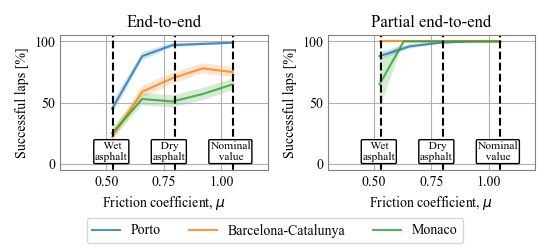
\includegraphics[width=\textwidth]{contents/chapt7/figs/mu/mu.png}
    %% Creator: Matplotlib, PGF backend
%%
%% To include the figure in your LaTeX document, write
%%   \input{<filename>.pgf}
%%
%% Make sure the required packages are loaded in your preamble
%%   \usepackage{pgf}
%%
%% Also ensure that all the required font packages are loaded; for instance,
%% the lmodern package is sometimes necessary when using math font.
%%   \usepackage{lmodern}
%%
%% Figures using additional raster images can only be included by \input if
%% they are in the same directory as the main LaTeX file. For loading figures
%% from other directories you can use the `import` package
%%   \usepackage{import}
%%
%% and then include the figures with
%%   \import{<path to file>}{<filename>.pgf}
%%
%% Matplotlib used the following preamble
%%   \usepackage{fontspec}
%%   \setmainfont{times.ttf}[Path=\detokenize{C:/Windows/Fonts/}]
%%   \setsansfont{DejaVuSans.ttf}[Path=\detokenize{C:/Users/Andrew/anaconda3/envs/auto_car_env/Lib/site-packages/matplotlib/mpl-data/fonts/ttf/}]
%%   \setmonofont{DejaVuSansMono.ttf}[Path=\detokenize{C:/Users/Andrew/anaconda3/envs/auto_car_env/Lib/site-packages/matplotlib/mpl-data/fonts/ttf/}]
%%
\begingroup%
\makeatletter%
\begin{pgfpicture}%
\pgfpathrectangle{\pgfpointorigin}{\pgfqpoint{5.700000in}{2.600000in}}%
\pgfusepath{use as bounding box, clip}%
\begin{pgfscope}%
\pgfsetbuttcap%
\pgfsetmiterjoin%
\definecolor{currentfill}{rgb}{1.000000,1.000000,1.000000}%
\pgfsetfillcolor{currentfill}%
\pgfsetlinewidth{0.000000pt}%
\definecolor{currentstroke}{rgb}{1.000000,1.000000,1.000000}%
\pgfsetstrokecolor{currentstroke}%
\pgfsetdash{}{0pt}%
\pgfpathmoveto{\pgfqpoint{0.000000in}{0.000000in}}%
\pgfpathlineto{\pgfqpoint{5.700000in}{0.000000in}}%
\pgfpathlineto{\pgfqpoint{5.700000in}{2.600000in}}%
\pgfpathlineto{\pgfqpoint{0.000000in}{2.600000in}}%
\pgfpathlineto{\pgfqpoint{0.000000in}{0.000000in}}%
\pgfpathclose%
\pgfusepath{fill}%
\end{pgfscope}%
\begin{pgfscope}%
\pgfsetbuttcap%
\pgfsetmiterjoin%
\definecolor{currentfill}{rgb}{1.000000,1.000000,1.000000}%
\pgfsetfillcolor{currentfill}%
\pgfsetlinewidth{0.000000pt}%
\definecolor{currentstroke}{rgb}{0.000000,0.000000,0.000000}%
\pgfsetstrokecolor{currentstroke}%
\pgfsetstrokeopacity{0.000000}%
\pgfsetdash{}{0pt}%
\pgfpathmoveto{\pgfqpoint{0.604167in}{1.040000in}}%
\pgfpathlineto{\pgfqpoint{2.775000in}{1.040000in}}%
\pgfpathlineto{\pgfqpoint{2.775000in}{2.246667in}}%
\pgfpathlineto{\pgfqpoint{0.604167in}{2.246667in}}%
\pgfpathlineto{\pgfqpoint{0.604167in}{1.040000in}}%
\pgfpathclose%
\pgfusepath{fill}%
\end{pgfscope}%
\begin{pgfscope}%
\pgfpathrectangle{\pgfqpoint{0.604167in}{1.040000in}}{\pgfqpoint{2.170833in}{1.206667in}}%
\pgfusepath{clip}%
\pgfsetbuttcap%
\pgfsetroundjoin%
\definecolor{currentfill}{rgb}{0.121569,0.466667,0.705882}%
\pgfsetfillcolor{currentfill}%
\pgfsetfillopacity{0.200000}%
\pgfsetlinewidth{0.000000pt}%
\definecolor{currentstroke}{rgb}{0.000000,0.000000,0.000000}%
\pgfsetstrokecolor{currentstroke}%
\pgfsetdash{}{0pt}%
\pgfpathmoveto{\pgfqpoint{1.145548in}{1.693898in}}%
\pgfpathlineto{\pgfqpoint{1.145548in}{1.793880in}}%
\pgfpathlineto{\pgfqpoint{1.461797in}{2.027954in}}%
\pgfpathlineto{\pgfqpoint{1.778045in}{2.164161in}}%
\pgfpathlineto{\pgfqpoint{2.094293in}{2.199206in}}%
\pgfpathlineto{\pgfqpoint{2.410541in}{2.196338in}}%
\pgfpathlineto{\pgfqpoint{2.410541in}{2.176328in}}%
\pgfpathlineto{\pgfqpoint{2.410541in}{2.176328in}}%
\pgfpathlineto{\pgfqpoint{2.094293in}{2.173460in}}%
\pgfpathlineto{\pgfqpoint{1.778045in}{2.128061in}}%
\pgfpathlineto{\pgfqpoint{1.461797in}{1.962601in}}%
\pgfpathlineto{\pgfqpoint{1.145548in}{1.693898in}}%
\pgfpathlineto{\pgfqpoint{1.145548in}{1.693898in}}%
\pgfpathclose%
\pgfusepath{fill}%
\end{pgfscope}%
\begin{pgfscope}%
\pgfpathrectangle{\pgfqpoint{0.604167in}{1.040000in}}{\pgfqpoint{2.170833in}{1.206667in}}%
\pgfusepath{clip}%
\pgfsetbuttcap%
\pgfsetroundjoin%
\definecolor{currentfill}{rgb}{1.000000,0.498039,0.054902}%
\pgfsetfillcolor{currentfill}%
\pgfsetfillopacity{0.200000}%
\pgfsetlinewidth{0.000000pt}%
\definecolor{currentstroke}{rgb}{0.000000,0.000000,0.000000}%
\pgfsetstrokecolor{currentstroke}%
\pgfsetdash{}{0pt}%
\pgfpathmoveto{\pgfqpoint{1.145548in}{1.206258in}}%
\pgfpathlineto{\pgfqpoint{1.145548in}{1.336298in}}%
\pgfpathlineto{\pgfqpoint{1.461797in}{1.648225in}}%
\pgfpathlineto{\pgfqpoint{1.778045in}{1.708688in}}%
\pgfpathlineto{\pgfqpoint{2.094293in}{1.868841in}}%
\pgfpathlineto{\pgfqpoint{2.410541in}{1.936655in}}%
\pgfpathlineto{\pgfqpoint{2.410541in}{1.792456in}}%
\pgfpathlineto{\pgfqpoint{2.410541in}{1.792456in}}%
\pgfpathlineto{\pgfqpoint{2.094293in}{1.719493in}}%
\pgfpathlineto{\pgfqpoint{1.778045in}{1.557868in}}%
\pgfpathlineto{\pgfqpoint{1.461797in}{1.497664in}}%
\pgfpathlineto{\pgfqpoint{1.145548in}{1.206258in}}%
\pgfpathlineto{\pgfqpoint{1.145548in}{1.206258in}}%
\pgfpathclose%
\pgfusepath{fill}%
\end{pgfscope}%
\begin{pgfscope}%
\pgfpathrectangle{\pgfqpoint{0.604167in}{1.040000in}}{\pgfqpoint{2.170833in}{1.206667in}}%
\pgfusepath{clip}%
\pgfsetbuttcap%
\pgfsetroundjoin%
\definecolor{currentfill}{rgb}{0.172549,0.627451,0.172549}%
\pgfsetfillcolor{currentfill}%
\pgfsetfillopacity{0.200000}%
\pgfsetlinewidth{0.000000pt}%
\definecolor{currentstroke}{rgb}{0.000000,0.000000,0.000000}%
\pgfsetstrokecolor{currentstroke}%
\pgfsetdash{}{0pt}%
\pgfpathmoveto{\pgfqpoint{1.145548in}{1.280129in}}%
\pgfpathlineto{\pgfqpoint{1.145548in}{1.362982in}}%
\pgfpathlineto{\pgfqpoint{1.461797in}{1.924005in}}%
\pgfpathlineto{\pgfqpoint{1.778045in}{2.061321in}}%
\pgfpathlineto{\pgfqpoint{2.094293in}{2.066871in}}%
\pgfpathlineto{\pgfqpoint{2.410541in}{2.068791in}}%
\pgfpathlineto{\pgfqpoint{2.410541in}{1.982098in}}%
\pgfpathlineto{\pgfqpoint{2.410541in}{1.982098in}}%
\pgfpathlineto{\pgfqpoint{2.094293in}{1.984018in}}%
\pgfpathlineto{\pgfqpoint{1.778045in}{1.969456in}}%
\pgfpathlineto{\pgfqpoint{1.461797in}{1.825217in}}%
\pgfpathlineto{\pgfqpoint{1.145548in}{1.280129in}}%
\pgfpathlineto{\pgfqpoint{1.145548in}{1.280129in}}%
\pgfpathclose%
\pgfusepath{fill}%
\end{pgfscope}%
\begin{pgfscope}%
\pgfpathrectangle{\pgfqpoint{0.604167in}{1.040000in}}{\pgfqpoint{2.170833in}{1.206667in}}%
\pgfusepath{clip}%
\pgfsetrectcap%
\pgfsetroundjoin%
\pgfsetlinewidth{0.803000pt}%
\definecolor{currentstroke}{rgb}{0.690196,0.690196,0.690196}%
\pgfsetstrokecolor{currentstroke}%
\pgfsetdash{}{0pt}%
\pgfpathmoveto{\pgfqpoint{0.845370in}{1.040000in}}%
\pgfpathlineto{\pgfqpoint{0.845370in}{2.246667in}}%
\pgfusepath{stroke}%
\end{pgfscope}%
\begin{pgfscope}%
\definecolor{textcolor}{rgb}{0.000000,0.000000,0.000000}%
\pgfsetstrokecolor{textcolor}%
\pgfsetfillcolor{textcolor}%
\pgftext[x=0.845370in,y=0.991389in,,top]{\color{textcolor}\rmfamily\fontsize{10.000000}{12.000000}\selectfont 0.4}%
\end{pgfscope}%
\begin{pgfscope}%
\pgfpathrectangle{\pgfqpoint{0.604167in}{1.040000in}}{\pgfqpoint{2.170833in}{1.206667in}}%
\pgfusepath{clip}%
\pgfsetrectcap%
\pgfsetroundjoin%
\pgfsetlinewidth{0.803000pt}%
\definecolor{currentstroke}{rgb}{0.690196,0.690196,0.690196}%
\pgfsetstrokecolor{currentstroke}%
\pgfsetdash{}{0pt}%
\pgfpathmoveto{\pgfqpoint{1.327778in}{1.040000in}}%
\pgfpathlineto{\pgfqpoint{1.327778in}{2.246667in}}%
\pgfusepath{stroke}%
\end{pgfscope}%
\begin{pgfscope}%
\definecolor{textcolor}{rgb}{0.000000,0.000000,0.000000}%
\pgfsetstrokecolor{textcolor}%
\pgfsetfillcolor{textcolor}%
\pgftext[x=1.327778in,y=0.991389in,,top]{\color{textcolor}\rmfamily\fontsize{10.000000}{12.000000}\selectfont 0.6}%
\end{pgfscope}%
\begin{pgfscope}%
\pgfpathrectangle{\pgfqpoint{0.604167in}{1.040000in}}{\pgfqpoint{2.170833in}{1.206667in}}%
\pgfusepath{clip}%
\pgfsetrectcap%
\pgfsetroundjoin%
\pgfsetlinewidth{0.803000pt}%
\definecolor{currentstroke}{rgb}{0.690196,0.690196,0.690196}%
\pgfsetstrokecolor{currentstroke}%
\pgfsetdash{}{0pt}%
\pgfpathmoveto{\pgfqpoint{1.810185in}{1.040000in}}%
\pgfpathlineto{\pgfqpoint{1.810185in}{2.246667in}}%
\pgfusepath{stroke}%
\end{pgfscope}%
\begin{pgfscope}%
\definecolor{textcolor}{rgb}{0.000000,0.000000,0.000000}%
\pgfsetstrokecolor{textcolor}%
\pgfsetfillcolor{textcolor}%
\pgftext[x=1.810185in,y=0.991389in,,top]{\color{textcolor}\rmfamily\fontsize{10.000000}{12.000000}\selectfont 0.8}%
\end{pgfscope}%
\begin{pgfscope}%
\pgfpathrectangle{\pgfqpoint{0.604167in}{1.040000in}}{\pgfqpoint{2.170833in}{1.206667in}}%
\pgfusepath{clip}%
\pgfsetrectcap%
\pgfsetroundjoin%
\pgfsetlinewidth{0.803000pt}%
\definecolor{currentstroke}{rgb}{0.690196,0.690196,0.690196}%
\pgfsetstrokecolor{currentstroke}%
\pgfsetdash{}{0pt}%
\pgfpathmoveto{\pgfqpoint{2.292593in}{1.040000in}}%
\pgfpathlineto{\pgfqpoint{2.292593in}{2.246667in}}%
\pgfusepath{stroke}%
\end{pgfscope}%
\begin{pgfscope}%
\definecolor{textcolor}{rgb}{0.000000,0.000000,0.000000}%
\pgfsetstrokecolor{textcolor}%
\pgfsetfillcolor{textcolor}%
\pgftext[x=2.292593in,y=0.991389in,,top]{\color{textcolor}\rmfamily\fontsize{10.000000}{12.000000}\selectfont 1.0}%
\end{pgfscope}%
\begin{pgfscope}%
\pgfpathrectangle{\pgfqpoint{0.604167in}{1.040000in}}{\pgfqpoint{2.170833in}{1.206667in}}%
\pgfusepath{clip}%
\pgfsetrectcap%
\pgfsetroundjoin%
\pgfsetlinewidth{0.803000pt}%
\definecolor{currentstroke}{rgb}{0.690196,0.690196,0.690196}%
\pgfsetstrokecolor{currentstroke}%
\pgfsetdash{}{0pt}%
\pgfpathmoveto{\pgfqpoint{2.775000in}{1.040000in}}%
\pgfpathlineto{\pgfqpoint{2.775000in}{2.246667in}}%
\pgfusepath{stroke}%
\end{pgfscope}%
\begin{pgfscope}%
\definecolor{textcolor}{rgb}{0.000000,0.000000,0.000000}%
\pgfsetstrokecolor{textcolor}%
\pgfsetfillcolor{textcolor}%
\pgftext[x=2.775000in,y=0.991389in,,top]{\color{textcolor}\rmfamily\fontsize{10.000000}{12.000000}\selectfont 1.2}%
\end{pgfscope}%
\begin{pgfscope}%
\definecolor{textcolor}{rgb}{0.000000,0.000000,0.000000}%
\pgfsetstrokecolor{textcolor}%
\pgfsetfillcolor{textcolor}%
\pgftext[x=1.689583in,y=0.809694in,,top]{\color{textcolor}\rmfamily\fontsize{10.000000}{12.000000}\selectfont Friction coefficient, \(\displaystyle \mu\)}%
\end{pgfscope}%
\begin{pgfscope}%
\pgfpathrectangle{\pgfqpoint{0.604167in}{1.040000in}}{\pgfqpoint{2.170833in}{1.206667in}}%
\pgfusepath{clip}%
\pgfsetrectcap%
\pgfsetroundjoin%
\pgfsetlinewidth{0.803000pt}%
\definecolor{currentstroke}{rgb}{0.690196,0.690196,0.690196}%
\pgfsetstrokecolor{currentstroke}%
\pgfsetdash{}{0pt}%
\pgfpathmoveto{\pgfqpoint{0.604167in}{1.190833in}}%
\pgfpathlineto{\pgfqpoint{2.775000in}{1.190833in}}%
\pgfusepath{stroke}%
\end{pgfscope}%
\begin{pgfscope}%
\definecolor{textcolor}{rgb}{0.000000,0.000000,0.000000}%
\pgfsetstrokecolor{textcolor}%
\pgfsetfillcolor{textcolor}%
\pgftext[x=0.486111in, y=1.142616in, left, base]{\color{textcolor}\rmfamily\fontsize{10.000000}{12.000000}\selectfont 0}%
\end{pgfscope}%
\begin{pgfscope}%
\pgfpathrectangle{\pgfqpoint{0.604167in}{1.040000in}}{\pgfqpoint{2.170833in}{1.206667in}}%
\pgfusepath{clip}%
\pgfsetrectcap%
\pgfsetroundjoin%
\pgfsetlinewidth{0.803000pt}%
\definecolor{currentstroke}{rgb}{0.690196,0.690196,0.690196}%
\pgfsetstrokecolor{currentstroke}%
\pgfsetdash{}{0pt}%
\pgfpathmoveto{\pgfqpoint{0.604167in}{1.693611in}}%
\pgfpathlineto{\pgfqpoint{2.775000in}{1.693611in}}%
\pgfusepath{stroke}%
\end{pgfscope}%
\begin{pgfscope}%
\definecolor{textcolor}{rgb}{0.000000,0.000000,0.000000}%
\pgfsetstrokecolor{textcolor}%
\pgfsetfillcolor{textcolor}%
\pgftext[x=0.416667in, y=1.645393in, left, base]{\color{textcolor}\rmfamily\fontsize{10.000000}{12.000000}\selectfont 50}%
\end{pgfscope}%
\begin{pgfscope}%
\pgfpathrectangle{\pgfqpoint{0.604167in}{1.040000in}}{\pgfqpoint{2.170833in}{1.206667in}}%
\pgfusepath{clip}%
\pgfsetrectcap%
\pgfsetroundjoin%
\pgfsetlinewidth{0.803000pt}%
\definecolor{currentstroke}{rgb}{0.690196,0.690196,0.690196}%
\pgfsetstrokecolor{currentstroke}%
\pgfsetdash{}{0pt}%
\pgfpathmoveto{\pgfqpoint{0.604167in}{2.196389in}}%
\pgfpathlineto{\pgfqpoint{2.775000in}{2.196389in}}%
\pgfusepath{stroke}%
\end{pgfscope}%
\begin{pgfscope}%
\definecolor{textcolor}{rgb}{0.000000,0.000000,0.000000}%
\pgfsetstrokecolor{textcolor}%
\pgfsetfillcolor{textcolor}%
\pgftext[x=0.347222in, y=2.148171in, left, base]{\color{textcolor}\rmfamily\fontsize{10.000000}{12.000000}\selectfont 100}%
\end{pgfscope}%
\begin{pgfscope}%
\definecolor{textcolor}{rgb}{0.000000,0.000000,0.000000}%
\pgfsetstrokecolor{textcolor}%
\pgfsetfillcolor{textcolor}%
\pgftext[x=0.291667in,y=1.643333in,,bottom,rotate=90.000000]{\color{textcolor}\rmfamily\fontsize{10.000000}{12.000000}\selectfont Successful laps [\%]}%
\end{pgfscope}%
\begin{pgfscope}%
\pgfpathrectangle{\pgfqpoint{0.604167in}{1.040000in}}{\pgfqpoint{2.170833in}{1.206667in}}%
\pgfusepath{clip}%
\pgfsetrectcap%
\pgfsetroundjoin%
\pgfsetlinewidth{1.505625pt}%
\definecolor{currentstroke}{rgb}{0.121569,0.466667,0.705882}%
\pgfsetstrokecolor{currentstroke}%
\pgfsetstrokeopacity{0.800000}%
\pgfsetdash{}{0pt}%
\pgfpathmoveto{\pgfqpoint{1.145548in}{1.743889in}}%
\pgfpathlineto{\pgfqpoint{1.461797in}{1.995278in}}%
\pgfpathlineto{\pgfqpoint{1.778045in}{2.146111in}}%
\pgfpathlineto{\pgfqpoint{2.094293in}{2.186333in}}%
\pgfpathlineto{\pgfqpoint{2.410541in}{2.186333in}}%
\pgfusepath{stroke}%
\end{pgfscope}%
\begin{pgfscope}%
\pgfpathrectangle{\pgfqpoint{0.604167in}{1.040000in}}{\pgfqpoint{2.170833in}{1.206667in}}%
\pgfusepath{clip}%
\pgfsetrectcap%
\pgfsetroundjoin%
\pgfsetlinewidth{1.505625pt}%
\definecolor{currentstroke}{rgb}{1.000000,0.498039,0.054902}%
\pgfsetstrokecolor{currentstroke}%
\pgfsetstrokeopacity{0.800000}%
\pgfsetdash{}{0pt}%
\pgfpathmoveto{\pgfqpoint{1.145548in}{1.271278in}}%
\pgfpathlineto{\pgfqpoint{1.461797in}{1.572944in}}%
\pgfpathlineto{\pgfqpoint{1.778045in}{1.633278in}}%
\pgfpathlineto{\pgfqpoint{2.094293in}{1.794167in}}%
\pgfpathlineto{\pgfqpoint{2.410541in}{1.864556in}}%
\pgfusepath{stroke}%
\end{pgfscope}%
\begin{pgfscope}%
\pgfpathrectangle{\pgfqpoint{0.604167in}{1.040000in}}{\pgfqpoint{2.170833in}{1.206667in}}%
\pgfusepath{clip}%
\pgfsetrectcap%
\pgfsetroundjoin%
\pgfsetlinewidth{1.505625pt}%
\definecolor{currentstroke}{rgb}{0.172549,0.627451,0.172549}%
\pgfsetstrokecolor{currentstroke}%
\pgfsetstrokeopacity{0.800000}%
\pgfsetdash{}{0pt}%
\pgfpathmoveto{\pgfqpoint{1.145548in}{1.321556in}}%
\pgfpathlineto{\pgfqpoint{1.461797in}{1.874611in}}%
\pgfpathlineto{\pgfqpoint{1.778045in}{2.015389in}}%
\pgfpathlineto{\pgfqpoint{2.094293in}{2.025444in}}%
\pgfpathlineto{\pgfqpoint{2.410541in}{2.025444in}}%
\pgfusepath{stroke}%
\end{pgfscope}%
\begin{pgfscope}%
\pgfpathrectangle{\pgfqpoint{0.604167in}{1.040000in}}{\pgfqpoint{2.170833in}{1.206667in}}%
\pgfusepath{clip}%
\pgfsetbuttcap%
\pgfsetroundjoin%
\pgfsetlinewidth{1.505625pt}%
\definecolor{currentstroke}{rgb}{0.000000,0.000000,0.000000}%
\pgfsetstrokecolor{currentstroke}%
\pgfsetdash{{5.550000pt}{2.400000pt}}{0.000000pt}%
\pgfpathmoveto{\pgfqpoint{2.410541in}{1.030000in}}%
\pgfpathlineto{\pgfqpoint{2.410541in}{2.256667in}}%
\pgfusepath{stroke}%
\end{pgfscope}%
\begin{pgfscope}%
\pgfpathrectangle{\pgfqpoint{0.604167in}{1.040000in}}{\pgfqpoint{2.170833in}{1.206667in}}%
\pgfusepath{clip}%
\pgfsetbuttcap%
\pgfsetroundjoin%
\pgfsetlinewidth{1.505625pt}%
\definecolor{currentstroke}{rgb}{0.000000,0.000000,0.000000}%
\pgfsetstrokecolor{currentstroke}%
\pgfsetdash{{5.550000pt}{2.400000pt}}{0.000000pt}%
\pgfpathmoveto{\pgfqpoint{1.810185in}{1.030000in}}%
\pgfpathlineto{\pgfqpoint{1.810185in}{2.256667in}}%
\pgfusepath{stroke}%
\end{pgfscope}%
\begin{pgfscope}%
\pgfpathrectangle{\pgfqpoint{0.604167in}{1.040000in}}{\pgfqpoint{2.170833in}{1.206667in}}%
\pgfusepath{clip}%
\pgfsetbuttcap%
\pgfsetroundjoin%
\pgfsetlinewidth{1.505625pt}%
\definecolor{currentstroke}{rgb}{0.000000,0.000000,0.000000}%
\pgfsetstrokecolor{currentstroke}%
\pgfsetdash{{5.550000pt}{2.400000pt}}{0.000000pt}%
\pgfpathmoveto{\pgfqpoint{1.158935in}{1.030000in}}%
\pgfpathlineto{\pgfqpoint{1.158935in}{2.256667in}}%
\pgfusepath{stroke}%
\end{pgfscope}%
\begin{pgfscope}%
\pgfsetrectcap%
\pgfsetmiterjoin%
\pgfsetlinewidth{0.803000pt}%
\definecolor{currentstroke}{rgb}{0.501961,0.501961,0.501961}%
\pgfsetstrokecolor{currentstroke}%
\pgfsetdash{}{0pt}%
\pgfpathmoveto{\pgfqpoint{0.604167in}{1.040000in}}%
\pgfpathlineto{\pgfqpoint{0.604167in}{2.246667in}}%
\pgfusepath{stroke}%
\end{pgfscope}%
\begin{pgfscope}%
\pgfsetrectcap%
\pgfsetmiterjoin%
\pgfsetlinewidth{0.803000pt}%
\definecolor{currentstroke}{rgb}{0.501961,0.501961,0.501961}%
\pgfsetstrokecolor{currentstroke}%
\pgfsetdash{}{0pt}%
\pgfpathmoveto{\pgfqpoint{2.775000in}{1.040000in}}%
\pgfpathlineto{\pgfqpoint{2.775000in}{2.246667in}}%
\pgfusepath{stroke}%
\end{pgfscope}%
\begin{pgfscope}%
\pgfsetrectcap%
\pgfsetmiterjoin%
\pgfsetlinewidth{0.803000pt}%
\definecolor{currentstroke}{rgb}{0.501961,0.501961,0.501961}%
\pgfsetstrokecolor{currentstroke}%
\pgfsetdash{}{0pt}%
\pgfpathmoveto{\pgfqpoint{0.604167in}{1.040000in}}%
\pgfpathlineto{\pgfqpoint{2.775000in}{1.040000in}}%
\pgfusepath{stroke}%
\end{pgfscope}%
\begin{pgfscope}%
\pgfsetrectcap%
\pgfsetmiterjoin%
\pgfsetlinewidth{0.803000pt}%
\definecolor{currentstroke}{rgb}{0.501961,0.501961,0.501961}%
\pgfsetstrokecolor{currentstroke}%
\pgfsetdash{}{0pt}%
\pgfpathmoveto{\pgfqpoint{0.604167in}{2.246667in}}%
\pgfpathlineto{\pgfqpoint{2.775000in}{2.246667in}}%
\pgfusepath{stroke}%
\end{pgfscope}%
\begin{pgfscope}%
\pgfsetbuttcap%
\pgfsetmiterjoin%
\definecolor{currentfill}{rgb}{1.000000,1.000000,1.000000}%
\pgfsetfillcolor{currentfill}%
\pgfsetlinewidth{1.003750pt}%
\definecolor{currentstroke}{rgb}{0.000000,0.000000,0.000000}%
\pgfsetstrokecolor{currentstroke}%
\pgfsetdash{}{0pt}%
\pgfpathmoveto{\pgfqpoint{2.171991in}{1.047018in}}%
\pgfpathlineto{\pgfqpoint{2.576865in}{1.047018in}}%
\pgfpathquadraticcurveto{\pgfqpoint{2.657851in}{1.047018in}}{\pgfqpoint{2.657851in}{1.128004in}}%
\pgfpathlineto{\pgfqpoint{2.657851in}{1.354218in}}%
\pgfpathquadraticcurveto{\pgfqpoint{2.657851in}{1.435204in}}{\pgfqpoint{2.576865in}{1.435204in}}%
\pgfpathlineto{\pgfqpoint{2.171991in}{1.435204in}}%
\pgfpathquadraticcurveto{\pgfqpoint{2.091005in}{1.435204in}}{\pgfqpoint{2.091005in}{1.354218in}}%
\pgfpathlineto{\pgfqpoint{2.091005in}{1.128004in}}%
\pgfpathquadraticcurveto{\pgfqpoint{2.091005in}{1.047018in}}{\pgfqpoint{2.171991in}{1.047018in}}%
\pgfpathlineto{\pgfqpoint{2.171991in}{1.047018in}}%
\pgfpathclose%
\pgfusepath{stroke,fill}%
\end{pgfscope}%
\begin{pgfscope}%
\definecolor{textcolor}{rgb}{0.000000,0.000000,0.000000}%
\pgfsetstrokecolor{textcolor}%
\pgfsetfillcolor{textcolor}%
\pgftext[x=2.171991in, y=1.273887in, left, base]{\color{textcolor}\rmfamily\fontsize{8.330000}{9.996000}\selectfont Nominal}%
\end{pgfscope}%
\begin{pgfscope}%
\definecolor{textcolor}{rgb}{0.000000,0.000000,0.000000}%
\pgfsetstrokecolor{textcolor}%
\pgfsetfillcolor{textcolor}%
\pgftext[x=2.171991in, y=1.152747in, left, base]{\color{textcolor}\rmfamily\fontsize{8.330000}{9.996000}\selectfont    value}%
\end{pgfscope}%
\begin{pgfscope}%
\pgfsetbuttcap%
\pgfsetmiterjoin%
\definecolor{currentfill}{rgb}{1.000000,1.000000,1.000000}%
\pgfsetfillcolor{currentfill}%
\pgfsetlinewidth{1.003750pt}%
\definecolor{currentstroke}{rgb}{0.000000,0.000000,0.000000}%
\pgfsetstrokecolor{currentstroke}%
\pgfsetdash{}{0pt}%
\pgfpathmoveto{\pgfqpoint{1.568981in}{1.047018in}}%
\pgfpathlineto{\pgfqpoint{1.896688in}{1.047018in}}%
\pgfpathquadraticcurveto{\pgfqpoint{1.977675in}{1.047018in}}{\pgfqpoint{1.977675in}{1.128004in}}%
\pgfpathlineto{\pgfqpoint{1.977675in}{1.354444in}}%
\pgfpathquadraticcurveto{\pgfqpoint{1.977675in}{1.435430in}}{\pgfqpoint{1.896688in}{1.435430in}}%
\pgfpathlineto{\pgfqpoint{1.568981in}{1.435430in}}%
\pgfpathquadraticcurveto{\pgfqpoint{1.487995in}{1.435430in}}{\pgfqpoint{1.487995in}{1.354444in}}%
\pgfpathlineto{\pgfqpoint{1.487995in}{1.128004in}}%
\pgfpathquadraticcurveto{\pgfqpoint{1.487995in}{1.047018in}}{\pgfqpoint{1.568981in}{1.047018in}}%
\pgfpathlineto{\pgfqpoint{1.568981in}{1.047018in}}%
\pgfpathclose%
\pgfusepath{stroke,fill}%
\end{pgfscope}%
\begin{pgfscope}%
\definecolor{textcolor}{rgb}{0.000000,0.000000,0.000000}%
\pgfsetstrokecolor{textcolor}%
\pgfsetfillcolor{textcolor}%
\pgftext[x=1.568981in, y=1.274113in, left, base]{\color{textcolor}\rmfamily\fontsize{8.330000}{9.996000}\selectfont    Dry}%
\end{pgfscope}%
\begin{pgfscope}%
\definecolor{textcolor}{rgb}{0.000000,0.000000,0.000000}%
\pgfsetstrokecolor{textcolor}%
\pgfsetfillcolor{textcolor}%
\pgftext[x=1.568981in, y=1.152747in, left, base]{\color{textcolor}\rmfamily\fontsize{8.330000}{9.996000}\selectfont asphalt}%
\end{pgfscope}%
\begin{pgfscope}%
\pgfsetbuttcap%
\pgfsetmiterjoin%
\definecolor{currentfill}{rgb}{1.000000,1.000000,1.000000}%
\pgfsetfillcolor{currentfill}%
\pgfsetlinewidth{1.003750pt}%
\definecolor{currentstroke}{rgb}{0.000000,0.000000,0.000000}%
\pgfsetstrokecolor{currentstroke}%
\pgfsetdash{}{0pt}%
\pgfpathmoveto{\pgfqpoint{0.965972in}{1.047018in}}%
\pgfpathlineto{\pgfqpoint{1.293679in}{1.047018in}}%
\pgfpathquadraticcurveto{\pgfqpoint{1.374665in}{1.047018in}}{\pgfqpoint{1.374665in}{1.128004in}}%
\pgfpathlineto{\pgfqpoint{1.374665in}{1.354218in}}%
\pgfpathquadraticcurveto{\pgfqpoint{1.374665in}{1.435204in}}{\pgfqpoint{1.293679in}{1.435204in}}%
\pgfpathlineto{\pgfqpoint{0.965972in}{1.435204in}}%
\pgfpathquadraticcurveto{\pgfqpoint{0.884986in}{1.435204in}}{\pgfqpoint{0.884986in}{1.354218in}}%
\pgfpathlineto{\pgfqpoint{0.884986in}{1.128004in}}%
\pgfpathquadraticcurveto{\pgfqpoint{0.884986in}{1.047018in}}{\pgfqpoint{0.965972in}{1.047018in}}%
\pgfpathlineto{\pgfqpoint{0.965972in}{1.047018in}}%
\pgfpathclose%
\pgfusepath{stroke,fill}%
\end{pgfscope}%
\begin{pgfscope}%
\definecolor{textcolor}{rgb}{0.000000,0.000000,0.000000}%
\pgfsetstrokecolor{textcolor}%
\pgfsetfillcolor{textcolor}%
\pgftext[x=0.965972in, y=1.273887in, left, base]{\color{textcolor}\rmfamily\fontsize{8.330000}{9.996000}\selectfont    Wet}%
\end{pgfscope}%
\begin{pgfscope}%
\definecolor{textcolor}{rgb}{0.000000,0.000000,0.000000}%
\pgfsetstrokecolor{textcolor}%
\pgfsetfillcolor{textcolor}%
\pgftext[x=0.965972in, y=1.152747in, left, base]{\color{textcolor}\rmfamily\fontsize{8.330000}{9.996000}\selectfont asphalt}%
\end{pgfscope}%
\begin{pgfscope}%
\definecolor{textcolor}{rgb}{0.000000,0.000000,0.000000}%
\pgfsetstrokecolor{textcolor}%
\pgfsetfillcolor{textcolor}%
\pgftext[x=1.689583in,y=2.330000in,,base]{\color{textcolor}\rmfamily\fontsize{12.000000}{14.400000}\selectfont End-to-end}%
\end{pgfscope}%
\begin{pgfscope}%
\pgfsetbuttcap%
\pgfsetmiterjoin%
\definecolor{currentfill}{rgb}{1.000000,1.000000,1.000000}%
\pgfsetfillcolor{currentfill}%
\pgfsetlinewidth{0.000000pt}%
\definecolor{currentstroke}{rgb}{0.000000,0.000000,0.000000}%
\pgfsetstrokecolor{currentstroke}%
\pgfsetstrokeopacity{0.000000}%
\pgfsetdash{}{0pt}%
\pgfpathmoveto{\pgfqpoint{3.379167in}{1.040000in}}%
\pgfpathlineto{\pgfqpoint{5.550000in}{1.040000in}}%
\pgfpathlineto{\pgfqpoint{5.550000in}{2.246667in}}%
\pgfpathlineto{\pgfqpoint{3.379167in}{2.246667in}}%
\pgfpathlineto{\pgfqpoint{3.379167in}{1.040000in}}%
\pgfpathclose%
\pgfusepath{fill}%
\end{pgfscope}%
\begin{pgfscope}%
\pgfpathrectangle{\pgfqpoint{3.379167in}{1.040000in}}{\pgfqpoint{2.170833in}{1.206667in}}%
\pgfusepath{clip}%
\pgfsetbuttcap%
\pgfsetroundjoin%
\definecolor{currentfill}{rgb}{0.121569,0.466667,0.705882}%
\pgfsetfillcolor{currentfill}%
\pgfsetfillopacity{0.200000}%
\pgfsetlinewidth{0.000000pt}%
\definecolor{currentstroke}{rgb}{0.000000,0.000000,0.000000}%
\pgfsetstrokecolor{currentstroke}%
\pgfsetdash{}{0pt}%
\pgfpathmoveto{\pgfqpoint{3.920548in}{2.032602in}}%
\pgfpathlineto{\pgfqpoint{3.920548in}{2.098731in}}%
\pgfpathlineto{\pgfqpoint{4.236797in}{2.185121in}}%
\pgfpathlineto{\pgfqpoint{4.553045in}{2.206394in}}%
\pgfpathlineto{\pgfqpoint{4.869293in}{2.202185in}}%
\pgfpathlineto{\pgfqpoint{5.185541in}{2.202185in}}%
\pgfpathlineto{\pgfqpoint{5.185541in}{2.190593in}}%
\pgfpathlineto{\pgfqpoint{5.185541in}{2.190593in}}%
\pgfpathlineto{\pgfqpoint{4.869293in}{2.190593in}}%
\pgfpathlineto{\pgfqpoint{4.553045in}{2.186384in}}%
\pgfpathlineto{\pgfqpoint{4.236797in}{2.147324in}}%
\pgfpathlineto{\pgfqpoint{3.920548in}{2.032602in}}%
\pgfpathlineto{\pgfqpoint{3.920548in}{2.032602in}}%
\pgfpathclose%
\pgfusepath{fill}%
\end{pgfscope}%
\begin{pgfscope}%
\pgfpathrectangle{\pgfqpoint{3.379167in}{1.040000in}}{\pgfqpoint{2.170833in}{1.206667in}}%
\pgfusepath{clip}%
\pgfsetbuttcap%
\pgfsetroundjoin%
\definecolor{currentfill}{rgb}{1.000000,0.498039,0.054902}%
\pgfsetfillcolor{currentfill}%
\pgfsetfillopacity{0.200000}%
\pgfsetlinewidth{0.000000pt}%
\definecolor{currentstroke}{rgb}{0.000000,0.000000,0.000000}%
\pgfsetstrokecolor{currentstroke}%
\pgfsetdash{}{0pt}%
\pgfpathmoveto{\pgfqpoint{3.920548in}{1.050728in}}%
\pgfpathlineto{\pgfqpoint{3.920548in}{1.351050in}}%
\pgfpathlineto{\pgfqpoint{3.971148in}{1.379169in}}%
\pgfpathlineto{\pgfqpoint{4.021748in}{1.865992in}}%
\pgfpathlineto{\pgfqpoint{4.072348in}{2.193719in}}%
\pgfpathlineto{\pgfqpoint{4.122947in}{2.202225in}}%
\pgfpathlineto{\pgfqpoint{4.173547in}{2.196389in}}%
\pgfpathlineto{\pgfqpoint{4.173547in}{2.196389in}}%
\pgfpathlineto{\pgfqpoint{4.173547in}{2.196389in}}%
\pgfpathlineto{\pgfqpoint{4.122947in}{2.170442in}}%
\pgfpathlineto{\pgfqpoint{4.072348in}{2.138725in}}%
\pgfpathlineto{\pgfqpoint{4.021748in}{1.662008in}}%
\pgfpathlineto{\pgfqpoint{3.971148in}{1.082942in}}%
\pgfpathlineto{\pgfqpoint{3.920548in}{1.050728in}}%
\pgfpathlineto{\pgfqpoint{3.920548in}{1.050728in}}%
\pgfpathclose%
\pgfusepath{fill}%
\end{pgfscope}%
\begin{pgfscope}%
\pgfpathrectangle{\pgfqpoint{3.379167in}{1.040000in}}{\pgfqpoint{2.170833in}{1.206667in}}%
\pgfusepath{clip}%
\pgfsetbuttcap%
\pgfsetroundjoin%
\definecolor{currentfill}{rgb}{0.172549,0.627451,0.172549}%
\pgfsetfillcolor{currentfill}%
\pgfsetfillopacity{0.200000}%
\pgfsetlinewidth{0.000000pt}%
\definecolor{currentstroke}{rgb}{0.000000,0.000000,0.000000}%
\pgfsetstrokecolor{currentstroke}%
\pgfsetdash{}{0pt}%
\pgfpathmoveto{\pgfqpoint{3.920548in}{2.196389in}}%
\pgfpathlineto{\pgfqpoint{3.920548in}{2.196389in}}%
\pgfpathlineto{\pgfqpoint{4.236797in}{2.196389in}}%
\pgfpathlineto{\pgfqpoint{4.553045in}{2.196389in}}%
\pgfpathlineto{\pgfqpoint{4.869293in}{2.196389in}}%
\pgfpathlineto{\pgfqpoint{5.185541in}{2.196389in}}%
\pgfpathlineto{\pgfqpoint{5.185541in}{2.196389in}}%
\pgfpathlineto{\pgfqpoint{5.185541in}{2.196389in}}%
\pgfpathlineto{\pgfqpoint{4.869293in}{2.196389in}}%
\pgfpathlineto{\pgfqpoint{4.553045in}{2.196389in}}%
\pgfpathlineto{\pgfqpoint{4.236797in}{2.196389in}}%
\pgfpathlineto{\pgfqpoint{3.920548in}{2.196389in}}%
\pgfpathlineto{\pgfqpoint{3.920548in}{2.196389in}}%
\pgfpathclose%
\pgfusepath{fill}%
\end{pgfscope}%
\begin{pgfscope}%
\pgfpathrectangle{\pgfqpoint{3.379167in}{1.040000in}}{\pgfqpoint{2.170833in}{1.206667in}}%
\pgfusepath{clip}%
\pgfsetrectcap%
\pgfsetroundjoin%
\pgfsetlinewidth{0.803000pt}%
\definecolor{currentstroke}{rgb}{0.690196,0.690196,0.690196}%
\pgfsetstrokecolor{currentstroke}%
\pgfsetdash{}{0pt}%
\pgfpathmoveto{\pgfqpoint{3.620370in}{1.040000in}}%
\pgfpathlineto{\pgfqpoint{3.620370in}{2.246667in}}%
\pgfusepath{stroke}%
\end{pgfscope}%
\begin{pgfscope}%
\definecolor{textcolor}{rgb}{0.000000,0.000000,0.000000}%
\pgfsetstrokecolor{textcolor}%
\pgfsetfillcolor{textcolor}%
\pgftext[x=3.620370in,y=0.991389in,,top]{\color{textcolor}\rmfamily\fontsize{10.000000}{12.000000}\selectfont 0.4}%
\end{pgfscope}%
\begin{pgfscope}%
\pgfpathrectangle{\pgfqpoint{3.379167in}{1.040000in}}{\pgfqpoint{2.170833in}{1.206667in}}%
\pgfusepath{clip}%
\pgfsetrectcap%
\pgfsetroundjoin%
\pgfsetlinewidth{0.803000pt}%
\definecolor{currentstroke}{rgb}{0.690196,0.690196,0.690196}%
\pgfsetstrokecolor{currentstroke}%
\pgfsetdash{}{0pt}%
\pgfpathmoveto{\pgfqpoint{4.102778in}{1.040000in}}%
\pgfpathlineto{\pgfqpoint{4.102778in}{2.246667in}}%
\pgfusepath{stroke}%
\end{pgfscope}%
\begin{pgfscope}%
\definecolor{textcolor}{rgb}{0.000000,0.000000,0.000000}%
\pgfsetstrokecolor{textcolor}%
\pgfsetfillcolor{textcolor}%
\pgftext[x=4.102778in,y=0.991389in,,top]{\color{textcolor}\rmfamily\fontsize{10.000000}{12.000000}\selectfont 0.6}%
\end{pgfscope}%
\begin{pgfscope}%
\pgfpathrectangle{\pgfqpoint{3.379167in}{1.040000in}}{\pgfqpoint{2.170833in}{1.206667in}}%
\pgfusepath{clip}%
\pgfsetrectcap%
\pgfsetroundjoin%
\pgfsetlinewidth{0.803000pt}%
\definecolor{currentstroke}{rgb}{0.690196,0.690196,0.690196}%
\pgfsetstrokecolor{currentstroke}%
\pgfsetdash{}{0pt}%
\pgfpathmoveto{\pgfqpoint{4.585185in}{1.040000in}}%
\pgfpathlineto{\pgfqpoint{4.585185in}{2.246667in}}%
\pgfusepath{stroke}%
\end{pgfscope}%
\begin{pgfscope}%
\definecolor{textcolor}{rgb}{0.000000,0.000000,0.000000}%
\pgfsetstrokecolor{textcolor}%
\pgfsetfillcolor{textcolor}%
\pgftext[x=4.585185in,y=0.991389in,,top]{\color{textcolor}\rmfamily\fontsize{10.000000}{12.000000}\selectfont 0.8}%
\end{pgfscope}%
\begin{pgfscope}%
\pgfpathrectangle{\pgfqpoint{3.379167in}{1.040000in}}{\pgfqpoint{2.170833in}{1.206667in}}%
\pgfusepath{clip}%
\pgfsetrectcap%
\pgfsetroundjoin%
\pgfsetlinewidth{0.803000pt}%
\definecolor{currentstroke}{rgb}{0.690196,0.690196,0.690196}%
\pgfsetstrokecolor{currentstroke}%
\pgfsetdash{}{0pt}%
\pgfpathmoveto{\pgfqpoint{5.067593in}{1.040000in}}%
\pgfpathlineto{\pgfqpoint{5.067593in}{2.246667in}}%
\pgfusepath{stroke}%
\end{pgfscope}%
\begin{pgfscope}%
\definecolor{textcolor}{rgb}{0.000000,0.000000,0.000000}%
\pgfsetstrokecolor{textcolor}%
\pgfsetfillcolor{textcolor}%
\pgftext[x=5.067593in,y=0.991389in,,top]{\color{textcolor}\rmfamily\fontsize{10.000000}{12.000000}\selectfont 1.0}%
\end{pgfscope}%
\begin{pgfscope}%
\pgfpathrectangle{\pgfqpoint{3.379167in}{1.040000in}}{\pgfqpoint{2.170833in}{1.206667in}}%
\pgfusepath{clip}%
\pgfsetrectcap%
\pgfsetroundjoin%
\pgfsetlinewidth{0.803000pt}%
\definecolor{currentstroke}{rgb}{0.690196,0.690196,0.690196}%
\pgfsetstrokecolor{currentstroke}%
\pgfsetdash{}{0pt}%
\pgfpathmoveto{\pgfqpoint{5.550000in}{1.040000in}}%
\pgfpathlineto{\pgfqpoint{5.550000in}{2.246667in}}%
\pgfusepath{stroke}%
\end{pgfscope}%
\begin{pgfscope}%
\definecolor{textcolor}{rgb}{0.000000,0.000000,0.000000}%
\pgfsetstrokecolor{textcolor}%
\pgfsetfillcolor{textcolor}%
\pgftext[x=5.550000in,y=0.991389in,,top]{\color{textcolor}\rmfamily\fontsize{10.000000}{12.000000}\selectfont 1.2}%
\end{pgfscope}%
\begin{pgfscope}%
\definecolor{textcolor}{rgb}{0.000000,0.000000,0.000000}%
\pgfsetstrokecolor{textcolor}%
\pgfsetfillcolor{textcolor}%
\pgftext[x=4.464583in,y=0.809694in,,top]{\color{textcolor}\rmfamily\fontsize{10.000000}{12.000000}\selectfont Friction coefficient, \(\displaystyle \mu\)}%
\end{pgfscope}%
\begin{pgfscope}%
\pgfpathrectangle{\pgfqpoint{3.379167in}{1.040000in}}{\pgfqpoint{2.170833in}{1.206667in}}%
\pgfusepath{clip}%
\pgfsetrectcap%
\pgfsetroundjoin%
\pgfsetlinewidth{0.803000pt}%
\definecolor{currentstroke}{rgb}{0.690196,0.690196,0.690196}%
\pgfsetstrokecolor{currentstroke}%
\pgfsetdash{}{0pt}%
\pgfpathmoveto{\pgfqpoint{3.379167in}{1.190833in}}%
\pgfpathlineto{\pgfqpoint{5.550000in}{1.190833in}}%
\pgfusepath{stroke}%
\end{pgfscope}%
\begin{pgfscope}%
\definecolor{textcolor}{rgb}{0.000000,0.000000,0.000000}%
\pgfsetstrokecolor{textcolor}%
\pgfsetfillcolor{textcolor}%
\pgftext[x=3.261111in, y=1.142616in, left, base]{\color{textcolor}\rmfamily\fontsize{10.000000}{12.000000}\selectfont 0}%
\end{pgfscope}%
\begin{pgfscope}%
\pgfpathrectangle{\pgfqpoint{3.379167in}{1.040000in}}{\pgfqpoint{2.170833in}{1.206667in}}%
\pgfusepath{clip}%
\pgfsetrectcap%
\pgfsetroundjoin%
\pgfsetlinewidth{0.803000pt}%
\definecolor{currentstroke}{rgb}{0.690196,0.690196,0.690196}%
\pgfsetstrokecolor{currentstroke}%
\pgfsetdash{}{0pt}%
\pgfpathmoveto{\pgfqpoint{3.379167in}{1.693611in}}%
\pgfpathlineto{\pgfqpoint{5.550000in}{1.693611in}}%
\pgfusepath{stroke}%
\end{pgfscope}%
\begin{pgfscope}%
\definecolor{textcolor}{rgb}{0.000000,0.000000,0.000000}%
\pgfsetstrokecolor{textcolor}%
\pgfsetfillcolor{textcolor}%
\pgftext[x=3.191667in, y=1.645393in, left, base]{\color{textcolor}\rmfamily\fontsize{10.000000}{12.000000}\selectfont 50}%
\end{pgfscope}%
\begin{pgfscope}%
\pgfpathrectangle{\pgfqpoint{3.379167in}{1.040000in}}{\pgfqpoint{2.170833in}{1.206667in}}%
\pgfusepath{clip}%
\pgfsetrectcap%
\pgfsetroundjoin%
\pgfsetlinewidth{0.803000pt}%
\definecolor{currentstroke}{rgb}{0.690196,0.690196,0.690196}%
\pgfsetstrokecolor{currentstroke}%
\pgfsetdash{}{0pt}%
\pgfpathmoveto{\pgfqpoint{3.379167in}{2.196389in}}%
\pgfpathlineto{\pgfqpoint{5.550000in}{2.196389in}}%
\pgfusepath{stroke}%
\end{pgfscope}%
\begin{pgfscope}%
\definecolor{textcolor}{rgb}{0.000000,0.000000,0.000000}%
\pgfsetstrokecolor{textcolor}%
\pgfsetfillcolor{textcolor}%
\pgftext[x=3.122222in, y=2.148171in, left, base]{\color{textcolor}\rmfamily\fontsize{10.000000}{12.000000}\selectfont 100}%
\end{pgfscope}%
\begin{pgfscope}%
\definecolor{textcolor}{rgb}{0.000000,0.000000,0.000000}%
\pgfsetstrokecolor{textcolor}%
\pgfsetfillcolor{textcolor}%
\pgftext[x=3.066667in,y=1.643333in,,bottom,rotate=90.000000]{\color{textcolor}\rmfamily\fontsize{10.000000}{12.000000}\selectfont Successful laps [\%]}%
\end{pgfscope}%
\begin{pgfscope}%
\pgfpathrectangle{\pgfqpoint{3.379167in}{1.040000in}}{\pgfqpoint{2.170833in}{1.206667in}}%
\pgfusepath{clip}%
\pgfsetrectcap%
\pgfsetroundjoin%
\pgfsetlinewidth{1.505625pt}%
\definecolor{currentstroke}{rgb}{0.121569,0.466667,0.705882}%
\pgfsetstrokecolor{currentstroke}%
\pgfsetstrokeopacity{0.800000}%
\pgfsetdash{}{0pt}%
\pgfpathmoveto{\pgfqpoint{3.920548in}{2.065667in}}%
\pgfpathlineto{\pgfqpoint{4.236797in}{2.166222in}}%
\pgfpathlineto{\pgfqpoint{4.553045in}{2.196389in}}%
\pgfpathlineto{\pgfqpoint{4.869293in}{2.196389in}}%
\pgfpathlineto{\pgfqpoint{5.185541in}{2.196389in}}%
\pgfusepath{stroke}%
\end{pgfscope}%
\begin{pgfscope}%
\pgfpathrectangle{\pgfqpoint{3.379167in}{1.040000in}}{\pgfqpoint{2.170833in}{1.206667in}}%
\pgfusepath{clip}%
\pgfsetrectcap%
\pgfsetroundjoin%
\pgfsetlinewidth{1.505625pt}%
\definecolor{currentstroke}{rgb}{1.000000,0.498039,0.054902}%
\pgfsetstrokecolor{currentstroke}%
\pgfsetstrokeopacity{0.800000}%
\pgfsetdash{}{0pt}%
\pgfpathmoveto{\pgfqpoint{3.920548in}{1.200889in}}%
\pgfpathlineto{\pgfqpoint{3.971148in}{1.231056in}}%
\pgfpathlineto{\pgfqpoint{4.021748in}{1.764000in}}%
\pgfpathlineto{\pgfqpoint{4.072348in}{2.166222in}}%
\pgfpathlineto{\pgfqpoint{4.122947in}{2.186333in}}%
\pgfpathlineto{\pgfqpoint{4.173547in}{2.196389in}}%
\pgfusepath{stroke}%
\end{pgfscope}%
\begin{pgfscope}%
\pgfpathrectangle{\pgfqpoint{3.379167in}{1.040000in}}{\pgfqpoint{2.170833in}{1.206667in}}%
\pgfusepath{clip}%
\pgfsetrectcap%
\pgfsetroundjoin%
\pgfsetlinewidth{1.505625pt}%
\definecolor{currentstroke}{rgb}{0.172549,0.627451,0.172549}%
\pgfsetstrokecolor{currentstroke}%
\pgfsetstrokeopacity{0.800000}%
\pgfsetdash{}{0pt}%
\pgfpathmoveto{\pgfqpoint{3.920548in}{2.196389in}}%
\pgfpathlineto{\pgfqpoint{4.236797in}{2.196389in}}%
\pgfpathlineto{\pgfqpoint{4.553045in}{2.196389in}}%
\pgfpathlineto{\pgfqpoint{4.869293in}{2.196389in}}%
\pgfpathlineto{\pgfqpoint{5.185541in}{2.196389in}}%
\pgfusepath{stroke}%
\end{pgfscope}%
\begin{pgfscope}%
\pgfpathrectangle{\pgfqpoint{3.379167in}{1.040000in}}{\pgfqpoint{2.170833in}{1.206667in}}%
\pgfusepath{clip}%
\pgfsetbuttcap%
\pgfsetroundjoin%
\pgfsetlinewidth{1.505625pt}%
\definecolor{currentstroke}{rgb}{0.000000,0.000000,0.000000}%
\pgfsetstrokecolor{currentstroke}%
\pgfsetdash{{5.550000pt}{2.400000pt}}{0.000000pt}%
\pgfpathmoveto{\pgfqpoint{5.185541in}{1.030000in}}%
\pgfpathlineto{\pgfqpoint{5.185541in}{2.256667in}}%
\pgfusepath{stroke}%
\end{pgfscope}%
\begin{pgfscope}%
\pgfpathrectangle{\pgfqpoint{3.379167in}{1.040000in}}{\pgfqpoint{2.170833in}{1.206667in}}%
\pgfusepath{clip}%
\pgfsetbuttcap%
\pgfsetroundjoin%
\pgfsetlinewidth{1.505625pt}%
\definecolor{currentstroke}{rgb}{0.000000,0.000000,0.000000}%
\pgfsetstrokecolor{currentstroke}%
\pgfsetdash{{5.550000pt}{2.400000pt}}{0.000000pt}%
\pgfpathmoveto{\pgfqpoint{4.585185in}{1.030000in}}%
\pgfpathlineto{\pgfqpoint{4.585185in}{2.256667in}}%
\pgfusepath{stroke}%
\end{pgfscope}%
\begin{pgfscope}%
\pgfpathrectangle{\pgfqpoint{3.379167in}{1.040000in}}{\pgfqpoint{2.170833in}{1.206667in}}%
\pgfusepath{clip}%
\pgfsetbuttcap%
\pgfsetroundjoin%
\pgfsetlinewidth{1.505625pt}%
\definecolor{currentstroke}{rgb}{0.000000,0.000000,0.000000}%
\pgfsetstrokecolor{currentstroke}%
\pgfsetdash{{5.550000pt}{2.400000pt}}{0.000000pt}%
\pgfpathmoveto{\pgfqpoint{3.933935in}{1.030000in}}%
\pgfpathlineto{\pgfqpoint{3.933935in}{2.256667in}}%
\pgfusepath{stroke}%
\end{pgfscope}%
\begin{pgfscope}%
\pgfsetrectcap%
\pgfsetmiterjoin%
\pgfsetlinewidth{0.803000pt}%
\definecolor{currentstroke}{rgb}{0.501961,0.501961,0.501961}%
\pgfsetstrokecolor{currentstroke}%
\pgfsetdash{}{0pt}%
\pgfpathmoveto{\pgfqpoint{3.379167in}{1.040000in}}%
\pgfpathlineto{\pgfqpoint{3.379167in}{2.246667in}}%
\pgfusepath{stroke}%
\end{pgfscope}%
\begin{pgfscope}%
\pgfsetrectcap%
\pgfsetmiterjoin%
\pgfsetlinewidth{0.803000pt}%
\definecolor{currentstroke}{rgb}{0.501961,0.501961,0.501961}%
\pgfsetstrokecolor{currentstroke}%
\pgfsetdash{}{0pt}%
\pgfpathmoveto{\pgfqpoint{5.550000in}{1.040000in}}%
\pgfpathlineto{\pgfqpoint{5.550000in}{2.246667in}}%
\pgfusepath{stroke}%
\end{pgfscope}%
\begin{pgfscope}%
\pgfsetrectcap%
\pgfsetmiterjoin%
\pgfsetlinewidth{0.803000pt}%
\definecolor{currentstroke}{rgb}{0.501961,0.501961,0.501961}%
\pgfsetstrokecolor{currentstroke}%
\pgfsetdash{}{0pt}%
\pgfpathmoveto{\pgfqpoint{3.379167in}{1.040000in}}%
\pgfpathlineto{\pgfqpoint{5.550000in}{1.040000in}}%
\pgfusepath{stroke}%
\end{pgfscope}%
\begin{pgfscope}%
\pgfsetrectcap%
\pgfsetmiterjoin%
\pgfsetlinewidth{0.803000pt}%
\definecolor{currentstroke}{rgb}{0.501961,0.501961,0.501961}%
\pgfsetstrokecolor{currentstroke}%
\pgfsetdash{}{0pt}%
\pgfpathmoveto{\pgfqpoint{3.379167in}{2.246667in}}%
\pgfpathlineto{\pgfqpoint{5.550000in}{2.246667in}}%
\pgfusepath{stroke}%
\end{pgfscope}%
\begin{pgfscope}%
\pgfsetbuttcap%
\pgfsetmiterjoin%
\definecolor{currentfill}{rgb}{1.000000,1.000000,1.000000}%
\pgfsetfillcolor{currentfill}%
\pgfsetlinewidth{1.003750pt}%
\definecolor{currentstroke}{rgb}{0.000000,0.000000,0.000000}%
\pgfsetstrokecolor{currentstroke}%
\pgfsetdash{}{0pt}%
\pgfpathmoveto{\pgfqpoint{4.946991in}{1.047018in}}%
\pgfpathlineto{\pgfqpoint{5.351865in}{1.047018in}}%
\pgfpathquadraticcurveto{\pgfqpoint{5.432851in}{1.047018in}}{\pgfqpoint{5.432851in}{1.128004in}}%
\pgfpathlineto{\pgfqpoint{5.432851in}{1.354218in}}%
\pgfpathquadraticcurveto{\pgfqpoint{5.432851in}{1.435204in}}{\pgfqpoint{5.351865in}{1.435204in}}%
\pgfpathlineto{\pgfqpoint{4.946991in}{1.435204in}}%
\pgfpathquadraticcurveto{\pgfqpoint{4.866005in}{1.435204in}}{\pgfqpoint{4.866005in}{1.354218in}}%
\pgfpathlineto{\pgfqpoint{4.866005in}{1.128004in}}%
\pgfpathquadraticcurveto{\pgfqpoint{4.866005in}{1.047018in}}{\pgfqpoint{4.946991in}{1.047018in}}%
\pgfpathlineto{\pgfqpoint{4.946991in}{1.047018in}}%
\pgfpathclose%
\pgfusepath{stroke,fill}%
\end{pgfscope}%
\begin{pgfscope}%
\definecolor{textcolor}{rgb}{0.000000,0.000000,0.000000}%
\pgfsetstrokecolor{textcolor}%
\pgfsetfillcolor{textcolor}%
\pgftext[x=4.946991in, y=1.273887in, left, base]{\color{textcolor}\rmfamily\fontsize{8.330000}{9.996000}\selectfont Nominal}%
\end{pgfscope}%
\begin{pgfscope}%
\definecolor{textcolor}{rgb}{0.000000,0.000000,0.000000}%
\pgfsetstrokecolor{textcolor}%
\pgfsetfillcolor{textcolor}%
\pgftext[x=4.946991in, y=1.152747in, left, base]{\color{textcolor}\rmfamily\fontsize{8.330000}{9.996000}\selectfont    value}%
\end{pgfscope}%
\begin{pgfscope}%
\pgfsetbuttcap%
\pgfsetmiterjoin%
\definecolor{currentfill}{rgb}{1.000000,1.000000,1.000000}%
\pgfsetfillcolor{currentfill}%
\pgfsetlinewidth{1.003750pt}%
\definecolor{currentstroke}{rgb}{0.000000,0.000000,0.000000}%
\pgfsetstrokecolor{currentstroke}%
\pgfsetdash{}{0pt}%
\pgfpathmoveto{\pgfqpoint{4.343981in}{1.047018in}}%
\pgfpathlineto{\pgfqpoint{4.671688in}{1.047018in}}%
\pgfpathquadraticcurveto{\pgfqpoint{4.752675in}{1.047018in}}{\pgfqpoint{4.752675in}{1.128004in}}%
\pgfpathlineto{\pgfqpoint{4.752675in}{1.354444in}}%
\pgfpathquadraticcurveto{\pgfqpoint{4.752675in}{1.435430in}}{\pgfqpoint{4.671688in}{1.435430in}}%
\pgfpathlineto{\pgfqpoint{4.343981in}{1.435430in}}%
\pgfpathquadraticcurveto{\pgfqpoint{4.262995in}{1.435430in}}{\pgfqpoint{4.262995in}{1.354444in}}%
\pgfpathlineto{\pgfqpoint{4.262995in}{1.128004in}}%
\pgfpathquadraticcurveto{\pgfqpoint{4.262995in}{1.047018in}}{\pgfqpoint{4.343981in}{1.047018in}}%
\pgfpathlineto{\pgfqpoint{4.343981in}{1.047018in}}%
\pgfpathclose%
\pgfusepath{stroke,fill}%
\end{pgfscope}%
\begin{pgfscope}%
\definecolor{textcolor}{rgb}{0.000000,0.000000,0.000000}%
\pgfsetstrokecolor{textcolor}%
\pgfsetfillcolor{textcolor}%
\pgftext[x=4.343981in, y=1.274113in, left, base]{\color{textcolor}\rmfamily\fontsize{8.330000}{9.996000}\selectfont    Dry}%
\end{pgfscope}%
\begin{pgfscope}%
\definecolor{textcolor}{rgb}{0.000000,0.000000,0.000000}%
\pgfsetstrokecolor{textcolor}%
\pgfsetfillcolor{textcolor}%
\pgftext[x=4.343981in, y=1.152747in, left, base]{\color{textcolor}\rmfamily\fontsize{8.330000}{9.996000}\selectfont asphalt}%
\end{pgfscope}%
\begin{pgfscope}%
\pgfsetbuttcap%
\pgfsetmiterjoin%
\definecolor{currentfill}{rgb}{1.000000,1.000000,1.000000}%
\pgfsetfillcolor{currentfill}%
\pgfsetlinewidth{1.003750pt}%
\definecolor{currentstroke}{rgb}{0.000000,0.000000,0.000000}%
\pgfsetstrokecolor{currentstroke}%
\pgfsetdash{}{0pt}%
\pgfpathmoveto{\pgfqpoint{3.740972in}{1.047018in}}%
\pgfpathlineto{\pgfqpoint{4.068679in}{1.047018in}}%
\pgfpathquadraticcurveto{\pgfqpoint{4.149665in}{1.047018in}}{\pgfqpoint{4.149665in}{1.128004in}}%
\pgfpathlineto{\pgfqpoint{4.149665in}{1.354218in}}%
\pgfpathquadraticcurveto{\pgfqpoint{4.149665in}{1.435204in}}{\pgfqpoint{4.068679in}{1.435204in}}%
\pgfpathlineto{\pgfqpoint{3.740972in}{1.435204in}}%
\pgfpathquadraticcurveto{\pgfqpoint{3.659986in}{1.435204in}}{\pgfqpoint{3.659986in}{1.354218in}}%
\pgfpathlineto{\pgfqpoint{3.659986in}{1.128004in}}%
\pgfpathquadraticcurveto{\pgfqpoint{3.659986in}{1.047018in}}{\pgfqpoint{3.740972in}{1.047018in}}%
\pgfpathlineto{\pgfqpoint{3.740972in}{1.047018in}}%
\pgfpathclose%
\pgfusepath{stroke,fill}%
\end{pgfscope}%
\begin{pgfscope}%
\definecolor{textcolor}{rgb}{0.000000,0.000000,0.000000}%
\pgfsetstrokecolor{textcolor}%
\pgfsetfillcolor{textcolor}%
\pgftext[x=3.740972in, y=1.273887in, left, base]{\color{textcolor}\rmfamily\fontsize{8.330000}{9.996000}\selectfont    Wet}%
\end{pgfscope}%
\begin{pgfscope}%
\definecolor{textcolor}{rgb}{0.000000,0.000000,0.000000}%
\pgfsetstrokecolor{textcolor}%
\pgfsetfillcolor{textcolor}%
\pgftext[x=3.740972in, y=1.152747in, left, base]{\color{textcolor}\rmfamily\fontsize{8.330000}{9.996000}\selectfont asphalt}%
\end{pgfscope}%
\begin{pgfscope}%
\definecolor{textcolor}{rgb}{0.000000,0.000000,0.000000}%
\pgfsetstrokecolor{textcolor}%
\pgfsetfillcolor{textcolor}%
\pgftext[x=4.464583in,y=2.330000in,,base]{\color{textcolor}\rmfamily\fontsize{12.000000}{14.400000}\selectfont Partial end-to-end}%
\end{pgfscope}%
\begin{pgfscope}%
\pgfsetbuttcap%
\pgfsetmiterjoin%
\definecolor{currentfill}{rgb}{1.000000,1.000000,1.000000}%
\pgfsetfillcolor{currentfill}%
\pgfsetfillopacity{0.800000}%
\pgfsetlinewidth{1.003750pt}%
\definecolor{currentstroke}{rgb}{0.800000,0.800000,0.800000}%
\pgfsetstrokecolor{currentstroke}%
\pgfsetstrokeopacity{0.800000}%
\pgfsetdash{}{0pt}%
\pgfpathmoveto{\pgfqpoint{0.913592in}{0.069444in}}%
\pgfpathlineto{\pgfqpoint{4.786408in}{0.069444in}}%
\pgfpathquadraticcurveto{\pgfqpoint{4.814186in}{0.069444in}}{\pgfqpoint{4.814186in}{0.097222in}}%
\pgfpathlineto{\pgfqpoint{4.814186in}{0.446642in}}%
\pgfpathquadraticcurveto{\pgfqpoint{4.814186in}{0.474419in}}{\pgfqpoint{4.786408in}{0.474419in}}%
\pgfpathlineto{\pgfqpoint{0.913592in}{0.474419in}}%
\pgfpathquadraticcurveto{\pgfqpoint{0.885814in}{0.474419in}}{\pgfqpoint{0.885814in}{0.446642in}}%
\pgfpathlineto{\pgfqpoint{0.885814in}{0.097222in}}%
\pgfpathquadraticcurveto{\pgfqpoint{0.885814in}{0.069444in}}{\pgfqpoint{0.913592in}{0.069444in}}%
\pgfpathlineto{\pgfqpoint{0.913592in}{0.069444in}}%
\pgfpathclose%
\pgfusepath{stroke,fill}%
\end{pgfscope}%
\begin{pgfscope}%
\pgfsetrectcap%
\pgfsetroundjoin%
\pgfsetlinewidth{1.505625pt}%
\definecolor{currentstroke}{rgb}{0.121569,0.466667,0.705882}%
\pgfsetstrokecolor{currentstroke}%
\pgfsetstrokeopacity{0.800000}%
\pgfsetdash{}{0pt}%
\pgfpathmoveto{\pgfqpoint{1.024703in}{0.286919in}}%
\pgfpathlineto{\pgfqpoint{1.163592in}{0.286919in}}%
\pgfpathlineto{\pgfqpoint{1.302481in}{0.286919in}}%
\pgfusepath{stroke}%
\end{pgfscope}%
\begin{pgfscope}%
\definecolor{textcolor}{rgb}{0.000000,0.000000,0.000000}%
\pgfsetstrokecolor{textcolor}%
\pgfsetfillcolor{textcolor}%
\pgftext[x=1.413592in,y=0.238308in,left,base]{\color{textcolor}\rmfamily\fontsize{10.000000}{12.000000}\selectfont Porto}%
\end{pgfscope}%
\begin{pgfscope}%
\pgfsetrectcap%
\pgfsetroundjoin%
\pgfsetlinewidth{1.505625pt}%
\definecolor{currentstroke}{rgb}{1.000000,0.498039,0.054902}%
\pgfsetstrokecolor{currentstroke}%
\pgfsetstrokeopacity{0.800000}%
\pgfsetdash{}{0pt}%
\pgfpathmoveto{\pgfqpoint{1.992341in}{0.286919in}}%
\pgfpathlineto{\pgfqpoint{2.131230in}{0.286919in}}%
\pgfpathlineto{\pgfqpoint{2.270119in}{0.286919in}}%
\pgfusepath{stroke}%
\end{pgfscope}%
\begin{pgfscope}%
\definecolor{textcolor}{rgb}{0.000000,0.000000,0.000000}%
\pgfsetstrokecolor{textcolor}%
\pgfsetfillcolor{textcolor}%
\pgftext[x=2.381230in,y=0.238308in,left,base]{\color{textcolor}\rmfamily\fontsize{10.000000}{12.000000}\selectfont Monaco}%
\end{pgfscope}%
\begin{pgfscope}%
\pgfsetrectcap%
\pgfsetroundjoin%
\pgfsetlinewidth{1.505625pt}%
\definecolor{currentstroke}{rgb}{0.172549,0.627451,0.172549}%
\pgfsetstrokecolor{currentstroke}%
\pgfsetstrokeopacity{0.800000}%
\pgfsetdash{}{0pt}%
\pgfpathmoveto{\pgfqpoint{3.114126in}{0.286919in}}%
\pgfpathlineto{\pgfqpoint{3.253015in}{0.286919in}}%
\pgfpathlineto{\pgfqpoint{3.391904in}{0.286919in}}%
\pgfusepath{stroke}%
\end{pgfscope}%
\begin{pgfscope}%
\definecolor{textcolor}{rgb}{0.000000,0.000000,0.000000}%
\pgfsetstrokecolor{textcolor}%
\pgfsetfillcolor{textcolor}%
\pgftext[x=3.503015in,y=0.238308in,left,base]{\color{textcolor}\rmfamily\fontsize{10.000000}{12.000000}\selectfont Barcelona-Catalunya}%
\end{pgfscope}%
\end{pgfpicture}%
\makeatother%
\endgroup%

    \caption[Success rate of agents under evaluation conditions with mismatched road surface friction coefficient]{Success rates under evaluation conditions of agents racing with decreased road surface friction values. Results for the end-to-end agent racing on all three tracks are shown in the left subplot, while results for the corresponding results for partial end-to-end agents are shown on the right. The values of friction corresponding to the nominal training value, dry, as well as wet asphalt are marked with a black dashed line.}
    \label{fig:mu}
\end{figure}


Figure \ref{fig:mu} illustrates the percentage of successful evaluation laps for both end-to-end and partial end-to-end agents when facing a mismatch in the road surface friction coefficient across all three tracks. 
Under nominal conditions, the end-to-end agents achieved success rates of $99\%$, $83\%$, and $61\%$ for Porto, Barcelona-Catalunya, and Monaco, respectively. However, when considering the worst-case scenario of racing on a wet asphalt surface, the success rates significantly decreased to $55\%$, $13\%$, and $8\%$ for these respective tracks.

On the other hand, the partial end-to-end agents successfully completed all their evaluation laps under nominal conditions. 
When a model mismatch in the road surface friction coefficient was introduced simulating a wet asphalt surface, the partial end-to-end agent was still able to complete all of its laps on Circuit de Barcelona-Catalunya.
However, it's success rate decreased to  $87\%$ and $6\%$ for the Porto and Monaco tracks.
The decrease in success rate for the partial end-to-end agent on Circuit de Monaco is especially severe.
However, we observe that only agents racing with a friction coefficient of less than $0.6$ crash at all. 

To investigate this large decrease in successful laps further, we observe  the locations where agents crashed while racing on a wet asphalt surface on the Monaco circuit, as depicted in Figure \ref{fig:mu_crash_locations}.
Apart from one crash, all the partial end-to-end agents failed at one of two corners.
Conversely, end-to-end agents crashed at various parts of the track while racing with a mismatched friction coefficient.

% Thus, partial end-to-end agents consistently outperformed the end-to-end agents regardless of the road surface conditions.
% Furthermore, the results under model mismatch conditions are consistent across all the tracks that were used in this investigation.

\begin{figure}[htb!]
    \centering
    % 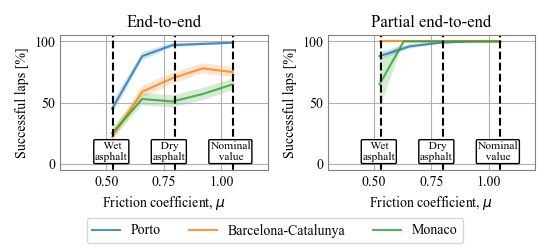
\includegraphics[width=\textwidth]{contents/chapt7/figs/mu/mu.png}
    %% Creator: Matplotlib, PGF backend
%%
%% To include the figure in your LaTeX document, write
%%   \input{<filename>.pgf}
%%
%% Make sure the required packages are loaded in your preamble
%%   \usepackage{pgf}
%%
%% Also ensure that all the required font packages are loaded; for instance,
%% the lmodern package is sometimes necessary when using math font.
%%   \usepackage{lmodern}
%%
%% Figures using additional raster images can only be included by \input if
%% they are in the same directory as the main LaTeX file. For loading figures
%% from other directories you can use the `import` package
%%   \usepackage{import}
%%
%% and then include the figures with
%%   \import{<path to file>}{<filename>.pgf}
%%
%% Matplotlib used the following preamble
%%   \usepackage{fontspec}
%%   \setmainfont{times.ttf}[Path=\detokenize{C:/Windows/Fonts/}]
%%   \setsansfont{DejaVuSans.ttf}[Path=\detokenize{C:/Users/Andrew/anaconda3/envs/auto_car_env/Lib/site-packages/matplotlib/mpl-data/fonts/ttf/}]
%%   \setmonofont{DejaVuSansMono.ttf}[Path=\detokenize{C:/Users/Andrew/anaconda3/envs/auto_car_env/Lib/site-packages/matplotlib/mpl-data/fonts/ttf/}]
%%
\begingroup%
\makeatletter%
\begin{pgfpicture}%
\pgfpathrectangle{\pgfpointorigin}{\pgfqpoint{5.500000in}{3.000000in}}%
\pgfusepath{use as bounding box, clip}%
\begin{pgfscope}%
\pgfsetbuttcap%
\pgfsetmiterjoin%
\definecolor{currentfill}{rgb}{1.000000,1.000000,1.000000}%
\pgfsetfillcolor{currentfill}%
\pgfsetlinewidth{0.000000pt}%
\definecolor{currentstroke}{rgb}{1.000000,1.000000,1.000000}%
\pgfsetstrokecolor{currentstroke}%
\pgfsetdash{}{0pt}%
\pgfpathmoveto{\pgfqpoint{0.000000in}{0.000000in}}%
\pgfpathlineto{\pgfqpoint{5.500000in}{0.000000in}}%
\pgfpathlineto{\pgfqpoint{5.500000in}{3.000000in}}%
\pgfpathlineto{\pgfqpoint{0.000000in}{3.000000in}}%
\pgfpathlineto{\pgfqpoint{0.000000in}{0.000000in}}%
\pgfpathclose%
\pgfusepath{fill}%
\end{pgfscope}%
\begin{pgfscope}%
\pgfpathrectangle{\pgfqpoint{1.176389in}{0.330000in}}{\pgfqpoint{2.459722in}{2.310000in}}%
\pgfusepath{clip}%
\pgfsys@transformshift{1.176389in}{0.330000in}%
\pgftext[left,bottom]{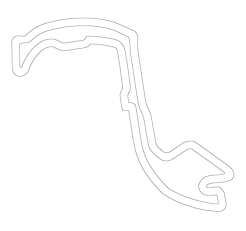
\includegraphics[interpolate=true,width=2.460000in,height=2.310000in]{contents/chapt7/figs/mu/mu_crash_locations-img0.png}}%
\end{pgfscope}%
\begin{pgfscope}%
\pgfpathrectangle{\pgfqpoint{1.176389in}{0.330000in}}{\pgfqpoint{2.459722in}{2.310000in}}%
\pgfusepath{clip}%
\pgfsetbuttcap%
\pgfsetroundjoin%
\definecolor{currentfill}{rgb}{0.121569,0.466667,0.705882}%
\pgfsetfillcolor{currentfill}%
\pgfsetlinewidth{1.003750pt}%
\definecolor{currentstroke}{rgb}{0.121569,0.466667,0.705882}%
\pgfsetstrokecolor{currentstroke}%
\pgfsetdash{}{0pt}%
\pgfsys@defobject{currentmarker}{\pgfqpoint{-0.041667in}{-0.041667in}}{\pgfqpoint{0.041667in}{0.041667in}}{%
\pgfpathmoveto{\pgfqpoint{-0.041667in}{-0.041667in}}%
\pgfpathlineto{\pgfqpoint{0.041667in}{0.041667in}}%
\pgfpathmoveto{\pgfqpoint{-0.041667in}{0.041667in}}%
\pgfpathlineto{\pgfqpoint{0.041667in}{-0.041667in}}%
\pgfusepath{stroke,fill}%
}%
\begin{pgfscope}%
\pgfsys@transformshift{1.396036in}{1.878103in}%
\pgfsys@useobject{currentmarker}{}%
\end{pgfscope}%
\begin{pgfscope}%
\pgfsys@transformshift{2.482649in}{1.393964in}%
\pgfsys@useobject{currentmarker}{}%
\end{pgfscope}%
\begin{pgfscope}%
\pgfsys@transformshift{3.134449in}{0.558345in}%
\pgfsys@useobject{currentmarker}{}%
\end{pgfscope}%
\begin{pgfscope}%
\pgfsys@transformshift{1.298295in}{2.003544in}%
\pgfsys@useobject{currentmarker}{}%
\end{pgfscope}%
\begin{pgfscope}%
\pgfsys@transformshift{1.410133in}{2.279145in}%
\pgfsys@useobject{currentmarker}{}%
\end{pgfscope}%
\begin{pgfscope}%
\pgfsys@transformshift{1.297804in}{1.966243in}%
\pgfsys@useobject{currentmarker}{}%
\end{pgfscope}%
\begin{pgfscope}%
\pgfsys@transformshift{3.399873in}{0.745512in}%
\pgfsys@useobject{currentmarker}{}%
\end{pgfscope}%
\begin{pgfscope}%
\pgfsys@transformshift{3.420315in}{0.704966in}%
\pgfsys@useobject{currentmarker}{}%
\end{pgfscope}%
\begin{pgfscope}%
\pgfsys@transformshift{1.298098in}{1.977844in}%
\pgfsys@useobject{currentmarker}{}%
\end{pgfscope}%
\begin{pgfscope}%
\pgfsys@transformshift{2.521542in}{1.169315in}%
\pgfsys@useobject{currentmarker}{}%
\end{pgfscope}%
\begin{pgfscope}%
\pgfsys@transformshift{1.296032in}{2.031845in}%
\pgfsys@useobject{currentmarker}{}%
\end{pgfscope}%
\begin{pgfscope}%
\pgfsys@transformshift{3.410279in}{0.817213in}%
\pgfsys@useobject{currentmarker}{}%
\end{pgfscope}%
\begin{pgfscope}%
\pgfsys@transformshift{3.424424in}{0.679446in}%
\pgfsys@useobject{currentmarker}{}%
\end{pgfscope}%
\begin{pgfscope}%
\pgfsys@transformshift{3.414302in}{0.722735in}%
\pgfsys@useobject{currentmarker}{}%
\end{pgfscope}%
\begin{pgfscope}%
\pgfsys@transformshift{1.408667in}{2.278595in}%
\pgfsys@useobject{currentmarker}{}%
\end{pgfscope}%
\begin{pgfscope}%
\pgfsys@transformshift{3.422868in}{0.690024in}%
\pgfsys@useobject{currentmarker}{}%
\end{pgfscope}%
\begin{pgfscope}%
\pgfsys@transformshift{1.298132in}{1.961858in}%
\pgfsys@useobject{currentmarker}{}%
\end{pgfscope}%
\begin{pgfscope}%
\pgfsys@transformshift{3.405813in}{0.736713in}%
\pgfsys@useobject{currentmarker}{}%
\end{pgfscope}%
\begin{pgfscope}%
\pgfsys@transformshift{3.188449in}{0.545970in}%
\pgfsys@useobject{currentmarker}{}%
\end{pgfscope}%
\begin{pgfscope}%
\pgfsys@transformshift{3.269952in}{0.532957in}%
\pgfsys@useobject{currentmarker}{}%
\end{pgfscope}%
\begin{pgfscope}%
\pgfsys@transformshift{3.422465in}{0.696170in}%
\pgfsys@useobject{currentmarker}{}%
\end{pgfscope}%
\begin{pgfscope}%
\pgfsys@transformshift{3.162132in}{1.197081in}%
\pgfsys@useobject{currentmarker}{}%
\end{pgfscope}%
\begin{pgfscope}%
\pgfsys@transformshift{3.231813in}{0.537294in}%
\pgfsys@useobject{currentmarker}{}%
\end{pgfscope}%
\begin{pgfscope}%
\pgfsys@transformshift{1.298011in}{1.983764in}%
\pgfsys@useobject{currentmarker}{}%
\end{pgfscope}%
\begin{pgfscope}%
\pgfsys@transformshift{3.413930in}{0.819517in}%
\pgfsys@useobject{currentmarker}{}%
\end{pgfscope}%
\begin{pgfscope}%
\pgfsys@transformshift{2.479359in}{1.615651in}%
\pgfsys@useobject{currentmarker}{}%
\end{pgfscope}%
\begin{pgfscope}%
\pgfsys@transformshift{3.378631in}{0.815528in}%
\pgfsys@useobject{currentmarker}{}%
\end{pgfscope}%
\begin{pgfscope}%
\pgfsys@transformshift{1.929670in}{2.458498in}%
\pgfsys@useobject{currentmarker}{}%
\end{pgfscope}%
\begin{pgfscope}%
\pgfsys@transformshift{3.269934in}{0.684828in}%
\pgfsys@useobject{currentmarker}{}%
\end{pgfscope}%
\begin{pgfscope}%
\pgfsys@transformshift{3.254992in}{0.533398in}%
\pgfsys@useobject{currentmarker}{}%
\end{pgfscope}%
\begin{pgfscope}%
\pgfsys@transformshift{2.501655in}{1.275406in}%
\pgfsys@useobject{currentmarker}{}%
\end{pgfscope}%
\begin{pgfscope}%
\pgfsys@transformshift{1.295920in}{2.019906in}%
\pgfsys@useobject{currentmarker}{}%
\end{pgfscope}%
\begin{pgfscope}%
\pgfsys@transformshift{1.296122in}{2.016654in}%
\pgfsys@useobject{currentmarker}{}%
\end{pgfscope}%
\begin{pgfscope}%
\pgfsys@transformshift{2.465570in}{1.616477in}%
\pgfsys@useobject{currentmarker}{}%
\end{pgfscope}%
\begin{pgfscope}%
\pgfsys@transformshift{3.422819in}{0.694843in}%
\pgfsys@useobject{currentmarker}{}%
\end{pgfscope}%
\begin{pgfscope}%
\pgfsys@transformshift{1.934654in}{2.458975in}%
\pgfsys@useobject{currentmarker}{}%
\end{pgfscope}%
\begin{pgfscope}%
\pgfsys@transformshift{1.758353in}{2.437115in}%
\pgfsys@useobject{currentmarker}{}%
\end{pgfscope}%
\begin{pgfscope}%
\pgfsys@transformshift{3.414102in}{0.722201in}%
\pgfsys@useobject{currentmarker}{}%
\end{pgfscope}%
\begin{pgfscope}%
\pgfsys@transformshift{2.465956in}{1.615800in}%
\pgfsys@useobject{currentmarker}{}%
\end{pgfscope}%
\begin{pgfscope}%
\pgfsys@transformshift{1.296160in}{2.037928in}%
\pgfsys@useobject{currentmarker}{}%
\end{pgfscope}%
\begin{pgfscope}%
\pgfsys@transformshift{1.298207in}{1.978519in}%
\pgfsys@useobject{currentmarker}{}%
\end{pgfscope}%
\begin{pgfscope}%
\pgfsys@transformshift{3.152688in}{0.554371in}%
\pgfsys@useobject{currentmarker}{}%
\end{pgfscope}%
\begin{pgfscope}%
\pgfsys@transformshift{3.422330in}{0.694893in}%
\pgfsys@useobject{currentmarker}{}%
\end{pgfscope}%
\begin{pgfscope}%
\pgfsys@transformshift{3.134155in}{1.216612in}%
\pgfsys@useobject{currentmarker}{}%
\end{pgfscope}%
\begin{pgfscope}%
\pgfsys@transformshift{2.478393in}{1.422615in}%
\pgfsys@useobject{currentmarker}{}%
\end{pgfscope}%
\begin{pgfscope}%
\pgfsys@transformshift{3.422308in}{0.691293in}%
\pgfsys@useobject{currentmarker}{}%
\end{pgfscope}%
\begin{pgfscope}%
\pgfsys@transformshift{3.276520in}{0.684773in}%
\pgfsys@useobject{currentmarker}{}%
\end{pgfscope}%
\begin{pgfscope}%
\pgfsys@transformshift{3.385071in}{0.815231in}%
\pgfsys@useobject{currentmarker}{}%
\end{pgfscope}%
\begin{pgfscope}%
\pgfsys@transformshift{3.401042in}{0.744024in}%
\pgfsys@useobject{currentmarker}{}%
\end{pgfscope}%
\begin{pgfscope}%
\pgfsys@transformshift{3.315926in}{0.687083in}%
\pgfsys@useobject{currentmarker}{}%
\end{pgfscope}%
\begin{pgfscope}%
\pgfsys@transformshift{3.427678in}{0.821425in}%
\pgfsys@useobject{currentmarker}{}%
\end{pgfscope}%
\begin{pgfscope}%
\pgfsys@transformshift{1.298285in}{1.984472in}%
\pgfsys@useobject{currentmarker}{}%
\end{pgfscope}%
\begin{pgfscope}%
\pgfsys@transformshift{2.527798in}{1.143520in}%
\pgfsys@useobject{currentmarker}{}%
\end{pgfscope}%
\begin{pgfscope}%
\pgfsys@transformshift{1.297537in}{1.978822in}%
\pgfsys@useobject{currentmarker}{}%
\end{pgfscope}%
\begin{pgfscope}%
\pgfsys@transformshift{3.410137in}{0.732113in}%
\pgfsys@useobject{currentmarker}{}%
\end{pgfscope}%
\begin{pgfscope}%
\pgfsys@transformshift{1.391705in}{2.280326in}%
\pgfsys@useobject{currentmarker}{}%
\end{pgfscope}%
\begin{pgfscope}%
\pgfsys@transformshift{3.422356in}{0.692925in}%
\pgfsys@useobject{currentmarker}{}%
\end{pgfscope}%
\begin{pgfscope}%
\pgfsys@transformshift{1.763783in}{2.437260in}%
\pgfsys@useobject{currentmarker}{}%
\end{pgfscope}%
\begin{pgfscope}%
\pgfsys@transformshift{3.383950in}{0.814970in}%
\pgfsys@useobject{currentmarker}{}%
\end{pgfscope}%
\begin{pgfscope}%
\pgfsys@transformshift{3.418291in}{0.714149in}%
\pgfsys@useobject{currentmarker}{}%
\end{pgfscope}%
\begin{pgfscope}%
\pgfsys@transformshift{3.300470in}{0.684815in}%
\pgfsys@useobject{currentmarker}{}%
\end{pgfscope}%
\begin{pgfscope}%
\pgfsys@transformshift{1.730541in}{2.430629in}%
\pgfsys@useobject{currentmarker}{}%
\end{pgfscope}%
\begin{pgfscope}%
\pgfsys@transformshift{3.424844in}{0.682985in}%
\pgfsys@useobject{currentmarker}{}%
\end{pgfscope}%
\begin{pgfscope}%
\pgfsys@transformshift{2.475922in}{1.435688in}%
\pgfsys@useobject{currentmarker}{}%
\end{pgfscope}%
\begin{pgfscope}%
\pgfsys@transformshift{2.488832in}{1.614716in}%
\pgfsys@useobject{currentmarker}{}%
\end{pgfscope}%
\begin{pgfscope}%
\pgfsys@transformshift{1.298023in}{2.004189in}%
\pgfsys@useobject{currentmarker}{}%
\end{pgfscope}%
\begin{pgfscope}%
\pgfsys@transformshift{3.397700in}{0.747985in}%
\pgfsys@useobject{currentmarker}{}%
\end{pgfscope}%
\begin{pgfscope}%
\pgfsys@transformshift{3.426953in}{0.667139in}%
\pgfsys@useobject{currentmarker}{}%
\end{pgfscope}%
\begin{pgfscope}%
\pgfsys@transformshift{3.380208in}{0.764270in}%
\pgfsys@useobject{currentmarker}{}%
\end{pgfscope}%
\begin{pgfscope}%
\pgfsys@transformshift{1.296166in}{2.044526in}%
\pgfsys@useobject{currentmarker}{}%
\end{pgfscope}%
\begin{pgfscope}%
\pgfsys@transformshift{2.493185in}{1.613907in}%
\pgfsys@useobject{currentmarker}{}%
\end{pgfscope}%
\begin{pgfscope}%
\pgfsys@transformshift{1.298031in}{1.965684in}%
\pgfsys@useobject{currentmarker}{}%
\end{pgfscope}%
\begin{pgfscope}%
\pgfsys@transformshift{2.492639in}{1.615018in}%
\pgfsys@useobject{currentmarker}{}%
\end{pgfscope}%
\begin{pgfscope}%
\pgfsys@transformshift{3.431824in}{1.003931in}%
\pgfsys@useobject{currentmarker}{}%
\end{pgfscope}%
\begin{pgfscope}%
\pgfsys@transformshift{3.420822in}{0.707979in}%
\pgfsys@useobject{currentmarker}{}%
\end{pgfscope}%
\begin{pgfscope}%
\pgfsys@transformshift{1.435461in}{2.208316in}%
\pgfsys@useobject{currentmarker}{}%
\end{pgfscope}%
\begin{pgfscope}%
\pgfsys@transformshift{3.424942in}{0.818973in}%
\pgfsys@useobject{currentmarker}{}%
\end{pgfscope}%
\begin{pgfscope}%
\pgfsys@transformshift{1.298030in}{1.985702in}%
\pgfsys@useobject{currentmarker}{}%
\end{pgfscope}%
\begin{pgfscope}%
\pgfsys@transformshift{3.308904in}{0.686172in}%
\pgfsys@useobject{currentmarker}{}%
\end{pgfscope}%
\begin{pgfscope}%
\pgfsys@transformshift{3.068332in}{0.575843in}%
\pgfsys@useobject{currentmarker}{}%
\end{pgfscope}%
\begin{pgfscope}%
\pgfsys@transformshift{2.503661in}{1.258027in}%
\pgfsys@useobject{currentmarker}{}%
\end{pgfscope}%
\begin{pgfscope}%
\pgfsys@transformshift{2.505859in}{1.242722in}%
\pgfsys@useobject{currentmarker}{}%
\end{pgfscope}%
\begin{pgfscope}%
\pgfsys@transformshift{2.390802in}{1.738043in}%
\pgfsys@useobject{currentmarker}{}%
\end{pgfscope}%
\begin{pgfscope}%
\pgfsys@transformshift{1.826986in}{2.367454in}%
\pgfsys@useobject{currentmarker}{}%
\end{pgfscope}%
\begin{pgfscope}%
\pgfsys@transformshift{3.423856in}{0.818732in}%
\pgfsys@useobject{currentmarker}{}%
\end{pgfscope}%
\begin{pgfscope}%
\pgfsys@transformshift{3.290385in}{0.684790in}%
\pgfsys@useobject{currentmarker}{}%
\end{pgfscope}%
\begin{pgfscope}%
\pgfsys@transformshift{3.143390in}{0.555097in}%
\pgfsys@useobject{currentmarker}{}%
\end{pgfscope}%
\begin{pgfscope}%
\pgfsys@transformshift{1.295983in}{2.025411in}%
\pgfsys@useobject{currentmarker}{}%
\end{pgfscope}%
\begin{pgfscope}%
\pgfsys@transformshift{3.364374in}{0.812899in}%
\pgfsys@useobject{currentmarker}{}%
\end{pgfscope}%
\begin{pgfscope}%
\pgfsys@transformshift{3.423513in}{0.819296in}%
\pgfsys@useobject{currentmarker}{}%
\end{pgfscope}%
\begin{pgfscope}%
\pgfsys@transformshift{3.119716in}{0.562421in}%
\pgfsys@useobject{currentmarker}{}%
\end{pgfscope}%
\begin{pgfscope}%
\pgfsys@transformshift{3.394494in}{0.815274in}%
\pgfsys@useobject{currentmarker}{}%
\end{pgfscope}%
\end{pgfscope}%
\begin{pgfscope}%
\pgfpathrectangle{\pgfqpoint{1.176389in}{0.330000in}}{\pgfqpoint{2.459722in}{2.310000in}}%
\pgfusepath{clip}%
\pgfsetbuttcap%
\pgfsetroundjoin%
\definecolor{currentfill}{rgb}{1.000000,0.498039,0.054902}%
\pgfsetfillcolor{currentfill}%
\pgfsetlinewidth{1.003750pt}%
\definecolor{currentstroke}{rgb}{1.000000,0.498039,0.054902}%
\pgfsetstrokecolor{currentstroke}%
\pgfsetdash{}{0pt}%
\pgfsys@defobject{currentmarker}{\pgfqpoint{-0.041667in}{-0.041667in}}{\pgfqpoint{0.041667in}{0.041667in}}{%
\pgfpathmoveto{\pgfqpoint{-0.041667in}{-0.041667in}}%
\pgfpathlineto{\pgfqpoint{0.041667in}{0.041667in}}%
\pgfpathmoveto{\pgfqpoint{-0.041667in}{0.041667in}}%
\pgfpathlineto{\pgfqpoint{0.041667in}{-0.041667in}}%
\pgfusepath{stroke,fill}%
}%
\begin{pgfscope}%
\pgfsys@transformshift{3.278789in}{0.685030in}%
\pgfsys@useobject{currentmarker}{}%
\end{pgfscope}%
\begin{pgfscope}%
\pgfsys@transformshift{1.389518in}{2.280750in}%
\pgfsys@useobject{currentmarker}{}%
\end{pgfscope}%
\begin{pgfscope}%
\pgfsys@transformshift{3.279434in}{0.684972in}%
\pgfsys@useobject{currentmarker}{}%
\end{pgfscope}%
\begin{pgfscope}%
\pgfsys@transformshift{1.391517in}{2.279271in}%
\pgfsys@useobject{currentmarker}{}%
\end{pgfscope}%
\begin{pgfscope}%
\pgfsys@transformshift{3.273383in}{0.684986in}%
\pgfsys@useobject{currentmarker}{}%
\end{pgfscope}%
\begin{pgfscope}%
\pgfsys@transformshift{3.276486in}{0.684882in}%
\pgfsys@useobject{currentmarker}{}%
\end{pgfscope}%
\begin{pgfscope}%
\pgfsys@transformshift{3.258596in}{0.684886in}%
\pgfsys@useobject{currentmarker}{}%
\end{pgfscope}%
\begin{pgfscope}%
\pgfsys@transformshift{1.392071in}{2.279440in}%
\pgfsys@useobject{currentmarker}{}%
\end{pgfscope}%
\begin{pgfscope}%
\pgfsys@transformshift{1.393842in}{2.278640in}%
\pgfsys@useobject{currentmarker}{}%
\end{pgfscope}%
\begin{pgfscope}%
\pgfsys@transformshift{1.395093in}{2.278641in}%
\pgfsys@useobject{currentmarker}{}%
\end{pgfscope}%
\begin{pgfscope}%
\pgfsys@transformshift{1.390369in}{2.278603in}%
\pgfsys@useobject{currentmarker}{}%
\end{pgfscope}%
\begin{pgfscope}%
\pgfsys@transformshift{3.266831in}{0.684990in}%
\pgfsys@useobject{currentmarker}{}%
\end{pgfscope}%
\begin{pgfscope}%
\pgfsys@transformshift{1.399708in}{2.278530in}%
\pgfsys@useobject{currentmarker}{}%
\end{pgfscope}%
\begin{pgfscope}%
\pgfsys@transformshift{1.394660in}{2.278761in}%
\pgfsys@useobject{currentmarker}{}%
\end{pgfscope}%
\begin{pgfscope}%
\pgfsys@transformshift{1.392901in}{2.278650in}%
\pgfsys@useobject{currentmarker}{}%
\end{pgfscope}%
\begin{pgfscope}%
\pgfsys@transformshift{1.411585in}{2.278668in}%
\pgfsys@useobject{currentmarker}{}%
\end{pgfscope}%
\begin{pgfscope}%
\pgfsys@transformshift{1.391977in}{2.280869in}%
\pgfsys@useobject{currentmarker}{}%
\end{pgfscope}%
\begin{pgfscope}%
\pgfsys@transformshift{1.391145in}{2.279328in}%
\pgfsys@useobject{currentmarker}{}%
\end{pgfscope}%
\begin{pgfscope}%
\pgfsys@transformshift{3.273575in}{0.684945in}%
\pgfsys@useobject{currentmarker}{}%
\end{pgfscope}%
\begin{pgfscope}%
\pgfsys@transformshift{3.265723in}{0.684749in}%
\pgfsys@useobject{currentmarker}{}%
\end{pgfscope}%
\begin{pgfscope}%
\pgfsys@transformshift{3.273915in}{0.684830in}%
\pgfsys@useobject{currentmarker}{}%
\end{pgfscope}%
\begin{pgfscope}%
\pgfsys@transformshift{1.390831in}{2.279446in}%
\pgfsys@useobject{currentmarker}{}%
\end{pgfscope}%
\begin{pgfscope}%
\pgfsys@transformshift{3.197548in}{0.849856in}%
\pgfsys@useobject{currentmarker}{}%
\end{pgfscope}%
\begin{pgfscope}%
\pgfsys@transformshift{1.399197in}{2.278758in}%
\pgfsys@useobject{currentmarker}{}%
\end{pgfscope}%
\begin{pgfscope}%
\pgfsys@transformshift{1.391710in}{2.279386in}%
\pgfsys@useobject{currentmarker}{}%
\end{pgfscope}%
\begin{pgfscope}%
\pgfsys@transformshift{1.402456in}{2.278685in}%
\pgfsys@useobject{currentmarker}{}%
\end{pgfscope}%
\begin{pgfscope}%
\pgfsys@transformshift{3.283424in}{0.684984in}%
\pgfsys@useobject{currentmarker}{}%
\end{pgfscope}%
\begin{pgfscope}%
\pgfsys@transformshift{1.390932in}{2.278610in}%
\pgfsys@useobject{currentmarker}{}%
\end{pgfscope}%
\begin{pgfscope}%
\pgfsys@transformshift{2.857945in}{1.029897in}%
\pgfsys@useobject{currentmarker}{}%
\end{pgfscope}%
\begin{pgfscope}%
\pgfsys@transformshift{1.391860in}{2.280497in}%
\pgfsys@useobject{currentmarker}{}%
\end{pgfscope}%
\begin{pgfscope}%
\pgfsys@transformshift{1.392033in}{2.280724in}%
\pgfsys@useobject{currentmarker}{}%
\end{pgfscope}%
\begin{pgfscope}%
\pgfsys@transformshift{3.273785in}{0.684955in}%
\pgfsys@useobject{currentmarker}{}%
\end{pgfscope}%
\begin{pgfscope}%
\pgfsys@transformshift{3.278942in}{0.685023in}%
\pgfsys@useobject{currentmarker}{}%
\end{pgfscope}%
\begin{pgfscope}%
\pgfsys@transformshift{1.390624in}{2.279112in}%
\pgfsys@useobject{currentmarker}{}%
\end{pgfscope}%
\begin{pgfscope}%
\pgfsys@transformshift{3.270040in}{0.685033in}%
\pgfsys@useobject{currentmarker}{}%
\end{pgfscope}%
\begin{pgfscope}%
\pgfsys@transformshift{1.398335in}{2.278591in}%
\pgfsys@useobject{currentmarker}{}%
\end{pgfscope}%
\begin{pgfscope}%
\pgfsys@transformshift{1.401511in}{2.278570in}%
\pgfsys@useobject{currentmarker}{}%
\end{pgfscope}%
\begin{pgfscope}%
\pgfsys@transformshift{2.853118in}{1.029144in}%
\pgfsys@useobject{currentmarker}{}%
\end{pgfscope}%
\begin{pgfscope}%
\pgfsys@transformshift{3.277040in}{0.685042in}%
\pgfsys@useobject{currentmarker}{}%
\end{pgfscope}%
\begin{pgfscope}%
\pgfsys@transformshift{1.413993in}{2.278620in}%
\pgfsys@useobject{currentmarker}{}%
\end{pgfscope}%
\begin{pgfscope}%
\pgfsys@transformshift{1.391423in}{2.279795in}%
\pgfsys@useobject{currentmarker}{}%
\end{pgfscope}%
\begin{pgfscope}%
\pgfsys@transformshift{3.272900in}{0.684964in}%
\pgfsys@useobject{currentmarker}{}%
\end{pgfscope}%
\begin{pgfscope}%
\pgfsys@transformshift{1.403472in}{2.278598in}%
\pgfsys@useobject{currentmarker}{}%
\end{pgfscope}%
\begin{pgfscope}%
\pgfsys@transformshift{3.271095in}{0.684983in}%
\pgfsys@useobject{currentmarker}{}%
\end{pgfscope}%
\begin{pgfscope}%
\pgfsys@transformshift{1.391793in}{2.279546in}%
\pgfsys@useobject{currentmarker}{}%
\end{pgfscope}%
\begin{pgfscope}%
\pgfsys@transformshift{1.391088in}{2.280104in}%
\pgfsys@useobject{currentmarker}{}%
\end{pgfscope}%
\begin{pgfscope}%
\pgfsys@transformshift{1.390957in}{2.279663in}%
\pgfsys@useobject{currentmarker}{}%
\end{pgfscope}%
\begin{pgfscope}%
\pgfsys@transformshift{3.270275in}{0.684851in}%
\pgfsys@useobject{currentmarker}{}%
\end{pgfscope}%
\begin{pgfscope}%
\pgfsys@transformshift{1.390617in}{2.280144in}%
\pgfsys@useobject{currentmarker}{}%
\end{pgfscope}%
\begin{pgfscope}%
\pgfsys@transformshift{1.413361in}{2.278536in}%
\pgfsys@useobject{currentmarker}{}%
\end{pgfscope}%
\begin{pgfscope}%
\pgfsys@transformshift{1.391390in}{2.278961in}%
\pgfsys@useobject{currentmarker}{}%
\end{pgfscope}%
\begin{pgfscope}%
\pgfsys@transformshift{3.270089in}{0.684728in}%
\pgfsys@useobject{currentmarker}{}%
\end{pgfscope}%
\begin{pgfscope}%
\pgfsys@transformshift{3.276646in}{0.684842in}%
\pgfsys@useobject{currentmarker}{}%
\end{pgfscope}%
\begin{pgfscope}%
\pgfsys@transformshift{1.409591in}{2.278594in}%
\pgfsys@useobject{currentmarker}{}%
\end{pgfscope}%
\begin{pgfscope}%
\pgfsys@transformshift{1.415967in}{2.278649in}%
\pgfsys@useobject{currentmarker}{}%
\end{pgfscope}%
\begin{pgfscope}%
\pgfsys@transformshift{3.277146in}{0.684969in}%
\pgfsys@useobject{currentmarker}{}%
\end{pgfscope}%
\begin{pgfscope}%
\pgfsys@transformshift{1.391557in}{2.280379in}%
\pgfsys@useobject{currentmarker}{}%
\end{pgfscope}%
\begin{pgfscope}%
\pgfsys@transformshift{3.271631in}{0.685000in}%
\pgfsys@useobject{currentmarker}{}%
\end{pgfscope}%
\begin{pgfscope}%
\pgfsys@transformshift{3.277066in}{0.685054in}%
\pgfsys@useobject{currentmarker}{}%
\end{pgfscope}%
\begin{pgfscope}%
\pgfsys@transformshift{1.406804in}{2.278636in}%
\pgfsys@useobject{currentmarker}{}%
\end{pgfscope}%
\begin{pgfscope}%
\pgfsys@transformshift{1.391842in}{2.280286in}%
\pgfsys@useobject{currentmarker}{}%
\end{pgfscope}%
\begin{pgfscope}%
\pgfsys@transformshift{1.390306in}{2.280510in}%
\pgfsys@useobject{currentmarker}{}%
\end{pgfscope}%
\begin{pgfscope}%
\pgfsys@transformshift{3.279039in}{0.684949in}%
\pgfsys@useobject{currentmarker}{}%
\end{pgfscope}%
\begin{pgfscope}%
\pgfsys@transformshift{3.310627in}{0.686739in}%
\pgfsys@useobject{currentmarker}{}%
\end{pgfscope}%
\begin{pgfscope}%
\pgfsys@transformshift{1.410290in}{2.278571in}%
\pgfsys@useobject{currentmarker}{}%
\end{pgfscope}%
\begin{pgfscope}%
\pgfsys@transformshift{1.390893in}{2.278885in}%
\pgfsys@useobject{currentmarker}{}%
\end{pgfscope}%
\begin{pgfscope}%
\pgfsys@transformshift{1.391507in}{2.278901in}%
\pgfsys@useobject{currentmarker}{}%
\end{pgfscope}%
\begin{pgfscope}%
\pgfsys@transformshift{3.270784in}{0.685005in}%
\pgfsys@useobject{currentmarker}{}%
\end{pgfscope}%
\begin{pgfscope}%
\pgfsys@transformshift{3.275161in}{0.684866in}%
\pgfsys@useobject{currentmarker}{}%
\end{pgfscope}%
\begin{pgfscope}%
\pgfsys@transformshift{1.391861in}{2.280126in}%
\pgfsys@useobject{currentmarker}{}%
\end{pgfscope}%
\begin{pgfscope}%
\pgfsys@transformshift{3.269374in}{0.684895in}%
\pgfsys@useobject{currentmarker}{}%
\end{pgfscope}%
\begin{pgfscope}%
\pgfsys@transformshift{1.391443in}{2.278838in}%
\pgfsys@useobject{currentmarker}{}%
\end{pgfscope}%
\begin{pgfscope}%
\pgfsys@transformshift{1.403254in}{2.278779in}%
\pgfsys@useobject{currentmarker}{}%
\end{pgfscope}%
\begin{pgfscope}%
\pgfsys@transformshift{1.391039in}{2.278699in}%
\pgfsys@useobject{currentmarker}{}%
\end{pgfscope}%
\begin{pgfscope}%
\pgfsys@transformshift{1.386194in}{2.280767in}%
\pgfsys@useobject{currentmarker}{}%
\end{pgfscope}%
\begin{pgfscope}%
\pgfsys@transformshift{3.271152in}{0.684741in}%
\pgfsys@useobject{currentmarker}{}%
\end{pgfscope}%
\begin{pgfscope}%
\pgfsys@transformshift{1.390399in}{2.280007in}%
\pgfsys@useobject{currentmarker}{}%
\end{pgfscope}%
\begin{pgfscope}%
\pgfsys@transformshift{1.416574in}{2.278796in}%
\pgfsys@useobject{currentmarker}{}%
\end{pgfscope}%
\begin{pgfscope}%
\pgfsys@transformshift{1.390530in}{2.279995in}%
\pgfsys@useobject{currentmarker}{}%
\end{pgfscope}%
\begin{pgfscope}%
\pgfsys@transformshift{3.284558in}{0.684927in}%
\pgfsys@useobject{currentmarker}{}%
\end{pgfscope}%
\begin{pgfscope}%
\pgfsys@transformshift{1.390667in}{2.278739in}%
\pgfsys@useobject{currentmarker}{}%
\end{pgfscope}%
\begin{pgfscope}%
\pgfsys@transformshift{1.393784in}{2.278592in}%
\pgfsys@useobject{currentmarker}{}%
\end{pgfscope}%
\begin{pgfscope}%
\pgfsys@transformshift{3.282342in}{0.685002in}%
\pgfsys@useobject{currentmarker}{}%
\end{pgfscope}%
\begin{pgfscope}%
\pgfsys@transformshift{1.393735in}{2.278664in}%
\pgfsys@useobject{currentmarker}{}%
\end{pgfscope}%
\begin{pgfscope}%
\pgfsys@transformshift{3.273085in}{0.684804in}%
\pgfsys@useobject{currentmarker}{}%
\end{pgfscope}%
\begin{pgfscope}%
\pgfsys@transformshift{1.390754in}{2.280239in}%
\pgfsys@useobject{currentmarker}{}%
\end{pgfscope}%
\begin{pgfscope}%
\pgfsys@transformshift{3.264842in}{0.685034in}%
\pgfsys@useobject{currentmarker}{}%
\end{pgfscope}%
\begin{pgfscope}%
\pgfsys@transformshift{1.392031in}{2.279011in}%
\pgfsys@useobject{currentmarker}{}%
\end{pgfscope}%
\begin{pgfscope}%
\pgfsys@transformshift{1.390286in}{2.279546in}%
\pgfsys@useobject{currentmarker}{}%
\end{pgfscope}%
\begin{pgfscope}%
\pgfsys@transformshift{1.394192in}{2.278825in}%
\pgfsys@useobject{currentmarker}{}%
\end{pgfscope}%
\begin{pgfscope}%
\pgfsys@transformshift{3.258717in}{0.684597in}%
\pgfsys@useobject{currentmarker}{}%
\end{pgfscope}%
\begin{pgfscope}%
\pgfsys@transformshift{3.273689in}{0.685031in}%
\pgfsys@useobject{currentmarker}{}%
\end{pgfscope}%
\begin{pgfscope}%
\pgfsys@transformshift{3.271560in}{0.684990in}%
\pgfsys@useobject{currentmarker}{}%
\end{pgfscope}%
\begin{pgfscope}%
\pgfsys@transformshift{3.269838in}{0.684783in}%
\pgfsys@useobject{currentmarker}{}%
\end{pgfscope}%
\end{pgfscope}%
\begin{pgfscope}%
\pgfsetbuttcap%
\pgfsetmiterjoin%
\definecolor{currentfill}{rgb}{1.000000,1.000000,1.000000}%
\pgfsetfillcolor{currentfill}%
\pgfsetfillopacity{0.800000}%
\pgfsetlinewidth{1.003750pt}%
\definecolor{currentstroke}{rgb}{0.800000,0.800000,0.800000}%
\pgfsetstrokecolor{currentstroke}%
\pgfsetstrokeopacity{0.800000}%
\pgfsetdash{}{0pt}%
\pgfpathmoveto{\pgfqpoint{3.765015in}{1.185574in}}%
\pgfpathlineto{\pgfqpoint{5.402778in}{1.185574in}}%
\pgfpathquadraticcurveto{\pgfqpoint{5.430556in}{1.185574in}}{\pgfqpoint{5.430556in}{1.213352in}}%
\pgfpathlineto{\pgfqpoint{5.430556in}{1.786648in}}%
\pgfpathquadraticcurveto{\pgfqpoint{5.430556in}{1.814426in}}{\pgfqpoint{5.402778in}{1.814426in}}%
\pgfpathlineto{\pgfqpoint{3.765015in}{1.814426in}}%
\pgfpathquadraticcurveto{\pgfqpoint{3.737237in}{1.814426in}}{\pgfqpoint{3.737237in}{1.786648in}}%
\pgfpathlineto{\pgfqpoint{3.737237in}{1.213352in}}%
\pgfpathquadraticcurveto{\pgfqpoint{3.737237in}{1.185574in}}{\pgfqpoint{3.765015in}{1.185574in}}%
\pgfpathlineto{\pgfqpoint{3.765015in}{1.185574in}}%
\pgfpathclose%
\pgfusepath{stroke,fill}%
\end{pgfscope}%
\begin{pgfscope}%
\pgfsetbuttcap%
\pgfsetroundjoin%
\definecolor{currentfill}{rgb}{0.121569,0.466667,0.705882}%
\pgfsetfillcolor{currentfill}%
\pgfsetlinewidth{1.003750pt}%
\definecolor{currentstroke}{rgb}{0.121569,0.466667,0.705882}%
\pgfsetstrokecolor{currentstroke}%
\pgfsetdash{}{0pt}%
\pgfsys@defobject{currentmarker}{\pgfqpoint{-0.041667in}{-0.041667in}}{\pgfqpoint{0.041667in}{0.041667in}}{%
\pgfpathmoveto{\pgfqpoint{-0.041667in}{-0.041667in}}%
\pgfpathlineto{\pgfqpoint{0.041667in}{0.041667in}}%
\pgfpathmoveto{\pgfqpoint{-0.041667in}{0.041667in}}%
\pgfpathlineto{\pgfqpoint{0.041667in}{-0.041667in}}%
\pgfusepath{stroke,fill}%
}%
\begin{pgfscope}%
\pgfsys@transformshift{4.028903in}{1.613037in}%
\pgfsys@useobject{currentmarker}{}%
\end{pgfscope}%
\end{pgfscope}%
\begin{pgfscope}%
\definecolor{textcolor}{rgb}{0.000000,0.000000,0.000000}%
\pgfsetstrokecolor{textcolor}%
\pgfsetfillcolor{textcolor}%
\pgftext[x=4.278903in,y=1.564426in,left,base]{\color{textcolor}\rmfamily\fontsize{10.000000}{12.000000}\selectfont End-to-end}%
\end{pgfscope}%
\begin{pgfscope}%
\pgfsetbuttcap%
\pgfsetroundjoin%
\definecolor{currentfill}{rgb}{1.000000,0.498039,0.054902}%
\pgfsetfillcolor{currentfill}%
\pgfsetlinewidth{1.003750pt}%
\definecolor{currentstroke}{rgb}{1.000000,0.498039,0.054902}%
\pgfsetstrokecolor{currentstroke}%
\pgfsetdash{}{0pt}%
\pgfsys@defobject{currentmarker}{\pgfqpoint{-0.041667in}{-0.041667in}}{\pgfqpoint{0.041667in}{0.041667in}}{%
\pgfpathmoveto{\pgfqpoint{-0.041667in}{-0.041667in}}%
\pgfpathlineto{\pgfqpoint{0.041667in}{0.041667in}}%
\pgfpathmoveto{\pgfqpoint{-0.041667in}{0.041667in}}%
\pgfpathlineto{\pgfqpoint{0.041667in}{-0.041667in}}%
\pgfusepath{stroke,fill}%
}%
\begin{pgfscope}%
\pgfsys@transformshift{4.028903in}{1.416667in}%
\pgfsys@useobject{currentmarker}{}%
\end{pgfscope}%
\end{pgfscope}%
\begin{pgfscope}%
\definecolor{textcolor}{rgb}{0.000000,0.000000,0.000000}%
\pgfsetstrokecolor{textcolor}%
\pgfsetfillcolor{textcolor}%
\pgftext[x=4.278903in,y=1.368056in,left,base]{\color{textcolor}\rmfamily\fontsize{10.000000}{12.000000}\selectfont Partial end-to-end}%
\end{pgfscope}%
\end{pgfpicture}%
\makeatother%
\endgroup%

    \caption[Locations where agents crashed while racing on a wet asphalt surface]{Locations where agents crashed while racing on a surface with a friction coefficient of $0.5$ (corresponding to wet asphalt).}
    \label{fig:mu_crash_locations}
\end{figure}

The fact that the partial end-to-end agent fails at only two locations on Circuit de Monaco when racing with a mismatched friction coefficient is an indicator that
it executes trajectories consistently.
To illustrate, an example of trajectories executed by both partial and fully end-to-end agents racing on a section of Circuit de Barcelona-Catalunya is shown in Figure \ref{fig:mu_lap}.
The figure shows the trajectories executed by agents under nominal conditions, as well as conditions with decreased surface friction.
Note that the trajectories executed by the partial end-to-end agent remain similar when mismatches are introduced.
The most notable difference between trajectories executed by the partial end-to-end agent on the nominal and slippier surfaces is that the trajectories executed on the slippier surfaces exhibit reduced curvature, resulting in wider paths being followed by the agents.
In contrast, the trajectories by the end-to-end agent are always erratic.
Thus, the partial end-to-end agent outperformed the end-to-end agent on the majority of road surface conditions.

\begin{figure}[htb!]
    \centering
    % 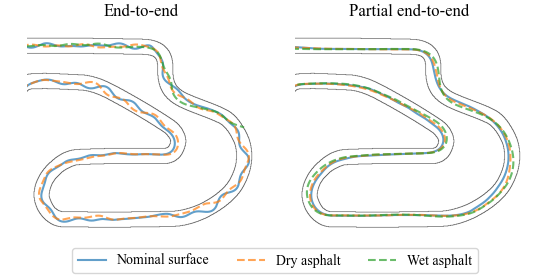
\includegraphics[width=\textwidth]{contents/chapt7/figs/mu/mu_lap.png}
    %% Creator: Matplotlib, PGF backend
%%
%% To include the figure in your LaTeX document, write
%%   \input{<filename>.pgf}
%%
%% Make sure the required packages are loaded in your preamble
%%   \usepackage{pgf}
%%
%% Also ensure that all the required font packages are loaded; for instance,
%% the lmodern package is sometimes necessary when using math font.
%%   \usepackage{lmodern}
%%
%% Figures using additional raster images can only be included by \input if
%% they are in the same directory as the main LaTeX file. For loading figures
%% from other directories you can use the `import` package
%%   \usepackage{import}
%%
%% and then include the figures with
%%   \import{<path to file>}{<filename>.pgf}
%%
%% Matplotlib used the following preamble
%%   \usepackage{fontspec}
%%   \setmainfont{times.ttf}[Path=\detokenize{C:/Windows/Fonts/}]
%%   \setsansfont{DejaVuSans.ttf}[Path=\detokenize{C:/Users/Andrew/anaconda3/envs/auto_car_env/Lib/site-packages/matplotlib/mpl-data/fonts/ttf/}]
%%   \setmonofont{DejaVuSansMono.ttf}[Path=\detokenize{C:/Users/Andrew/anaconda3/envs/auto_car_env/Lib/site-packages/matplotlib/mpl-data/fonts/ttf/}]
%%
\begingroup%
\makeatletter%
\begin{pgfpicture}%
\pgfpathrectangle{\pgfpointorigin}{\pgfqpoint{5.500000in}{2.800000in}}%
\pgfusepath{use as bounding box, clip}%
\begin{pgfscope}%
\pgfsetbuttcap%
\pgfsetmiterjoin%
\definecolor{currentfill}{rgb}{1.000000,1.000000,1.000000}%
\pgfsetfillcolor{currentfill}%
\pgfsetlinewidth{0.000000pt}%
\definecolor{currentstroke}{rgb}{1.000000,1.000000,1.000000}%
\pgfsetstrokecolor{currentstroke}%
\pgfsetdash{}{0pt}%
\pgfpathmoveto{\pgfqpoint{0.000000in}{0.000000in}}%
\pgfpathlineto{\pgfqpoint{5.500000in}{0.000000in}}%
\pgfpathlineto{\pgfqpoint{5.500000in}{2.800000in}}%
\pgfpathlineto{\pgfqpoint{0.000000in}{2.800000in}}%
\pgfpathlineto{\pgfqpoint{0.000000in}{0.000000in}}%
\pgfpathclose%
\pgfusepath{fill}%
\end{pgfscope}%
\begin{pgfscope}%
\pgfpathrectangle{\pgfqpoint{0.316542in}{0.364000in}}{\pgfqpoint{2.191917in}{2.191917in}}%
\pgfusepath{clip}%
\pgfsys@transformshift{0.316542in}{0.364000in}%
\pgftext[left,bottom]{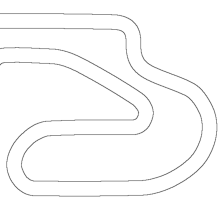
\includegraphics[interpolate=true,width=2.200000in,height=2.200000in]{contents/chapt7/figs/mu/mu_lap_1-img0.png}}%
\end{pgfscope}%
\begin{pgfscope}%
\pgfpathrectangle{\pgfqpoint{0.316542in}{0.364000in}}{\pgfqpoint{2.191917in}{2.191917in}}%
\pgfusepath{clip}%
\pgfsetbuttcap%
\pgfsetroundjoin%
\pgfsetlinewidth{1.505625pt}%
\definecolor{currentstroke}{rgb}{1.000000,0.000000,0.000000}%
\pgfsetstrokecolor{currentstroke}%
\pgfsetdash{{1.500000pt}{2.475000pt}}{0.000000pt}%
\pgfusepath{stroke}%
\end{pgfscope}%
\begin{pgfscope}%
\pgfpathrectangle{\pgfqpoint{0.316542in}{0.364000in}}{\pgfqpoint{2.191917in}{2.191917in}}%
\pgfusepath{clip}%
\pgfsetrectcap%
\pgfsetroundjoin%
\pgfsetlinewidth{1.505625pt}%
\definecolor{currentstroke}{rgb}{0.121569,0.466667,0.705882}%
\pgfsetstrokecolor{currentstroke}%
\pgfsetstrokeopacity{0.700000}%
\pgfsetdash{}{0pt}%
\pgfpathmoveto{\pgfqpoint{0.306542in}{2.373041in}}%
\pgfpathlineto{\pgfqpoint{0.329574in}{2.372585in}}%
\pgfpathlineto{\pgfqpoint{0.357863in}{2.369488in}}%
\pgfpathlineto{\pgfqpoint{0.414323in}{2.362345in}}%
\pgfpathlineto{\pgfqpoint{0.438709in}{2.362056in}}%
\pgfpathlineto{\pgfqpoint{0.458943in}{2.363871in}}%
\pgfpathlineto{\pgfqpoint{0.486888in}{2.368803in}}%
\pgfpathlineto{\pgfqpoint{0.521605in}{2.374847in}}%
\pgfpathlineto{\pgfqpoint{0.540799in}{2.375906in}}%
\pgfpathlineto{\pgfqpoint{0.560153in}{2.374446in}}%
\pgfpathlineto{\pgfqpoint{0.579771in}{2.370258in}}%
\pgfpathlineto{\pgfqpoint{0.603153in}{2.362821in}}%
\pgfpathlineto{\pgfqpoint{0.645796in}{2.348508in}}%
\pgfpathlineto{\pgfqpoint{0.665813in}{2.344377in}}%
\pgfpathlineto{\pgfqpoint{0.682117in}{2.343128in}}%
\pgfpathlineto{\pgfqpoint{0.698449in}{2.343931in}}%
\pgfpathlineto{\pgfqpoint{0.718569in}{2.347522in}}%
\pgfpathlineto{\pgfqpoint{0.742125in}{2.354389in}}%
\pgfpathlineto{\pgfqpoint{0.777408in}{2.364842in}}%
\pgfpathlineto{\pgfqpoint{0.797580in}{2.368125in}}%
\pgfpathlineto{\pgfqpoint{0.813925in}{2.368633in}}%
\pgfpathlineto{\pgfqpoint{0.834267in}{2.366664in}}%
\pgfpathlineto{\pgfqpoint{0.858245in}{2.361474in}}%
\pgfpathlineto{\pgfqpoint{0.902036in}{2.351221in}}%
\pgfpathlineto{\pgfqpoint{0.922367in}{2.349112in}}%
\pgfpathlineto{\pgfqpoint{0.942804in}{2.349475in}}%
\pgfpathlineto{\pgfqpoint{0.967145in}{2.352546in}}%
\pgfpathlineto{\pgfqpoint{1.019719in}{2.360378in}}%
\pgfpathlineto{\pgfqpoint{1.044234in}{2.361326in}}%
\pgfpathlineto{\pgfqpoint{1.072821in}{2.359834in}}%
\pgfpathlineto{\pgfqpoint{1.125883in}{2.356561in}}%
\pgfpathlineto{\pgfqpoint{1.158594in}{2.357274in}}%
\pgfpathlineto{\pgfqpoint{1.236244in}{2.360136in}}%
\pgfpathlineto{\pgfqpoint{1.350712in}{2.360019in}}%
\pgfpathlineto{\pgfqpoint{1.403822in}{2.362436in}}%
\pgfpathlineto{\pgfqpoint{1.432415in}{2.361132in}}%
\pgfpathlineto{\pgfqpoint{1.456698in}{2.357640in}}%
\pgfpathlineto{\pgfqpoint{1.476521in}{2.352647in}}%
\pgfpathlineto{\pgfqpoint{1.495642in}{2.345427in}}%
\pgfpathlineto{\pgfqpoint{1.510070in}{2.337734in}}%
\pgfpathlineto{\pgfqpoint{1.523228in}{2.328036in}}%
\pgfpathlineto{\pgfqpoint{1.534652in}{2.316347in}}%
\pgfpathlineto{\pgfqpoint{1.544053in}{2.302975in}}%
\pgfpathlineto{\pgfqpoint{1.551402in}{2.288370in}}%
\pgfpathlineto{\pgfqpoint{1.558194in}{2.269090in}}%
\pgfpathlineto{\pgfqpoint{1.576185in}{2.210514in}}%
\pgfpathlineto{\pgfqpoint{1.583777in}{2.196030in}}%
\pgfpathlineto{\pgfqpoint{1.595447in}{2.179252in}}%
\pgfpathlineto{\pgfqpoint{1.611718in}{2.160891in}}%
\pgfpathlineto{\pgfqpoint{1.638641in}{2.131481in}}%
\pgfpathlineto{\pgfqpoint{1.647009in}{2.118971in}}%
\pgfpathlineto{\pgfqpoint{1.653480in}{2.105020in}}%
\pgfpathlineto{\pgfqpoint{1.658087in}{2.089776in}}%
\pgfpathlineto{\pgfqpoint{1.661718in}{2.069772in}}%
\pgfpathlineto{\pgfqpoint{1.665781in}{2.029299in}}%
\pgfpathlineto{\pgfqpoint{1.669705in}{2.005221in}}%
\pgfpathlineto{\pgfqpoint{1.674207in}{1.989594in}}%
\pgfpathlineto{\pgfqpoint{1.680793in}{1.974731in}}%
\pgfpathlineto{\pgfqpoint{1.689635in}{1.961091in}}%
\pgfpathlineto{\pgfqpoint{1.700539in}{1.949035in}}%
\pgfpathlineto{\pgfqpoint{1.713066in}{1.938667in}}%
\pgfpathlineto{\pgfqpoint{1.730222in}{1.927759in}}%
\pgfpathlineto{\pgfqpoint{1.797215in}{1.889405in}}%
\pgfpathlineto{\pgfqpoint{1.816020in}{1.873861in}}%
\pgfpathlineto{\pgfqpoint{1.836279in}{1.853856in}}%
\pgfpathlineto{\pgfqpoint{1.862338in}{1.828152in}}%
\pgfpathlineto{\pgfqpoint{1.878082in}{1.815285in}}%
\pgfpathlineto{\pgfqpoint{1.895050in}{1.804085in}}%
\pgfpathlineto{\pgfqpoint{1.913050in}{1.794632in}}%
\pgfpathlineto{\pgfqpoint{1.935630in}{1.785381in}}%
\pgfpathlineto{\pgfqpoint{1.970455in}{1.774099in}}%
\pgfpathlineto{\pgfqpoint{2.024617in}{1.756515in}}%
\pgfpathlineto{\pgfqpoint{2.077772in}{1.736075in}}%
\pgfpathlineto{\pgfqpoint{2.164452in}{1.701003in}}%
\pgfpathlineto{\pgfqpoint{2.182005in}{1.690740in}}%
\pgfpathlineto{\pgfqpoint{2.201798in}{1.676473in}}%
\pgfpathlineto{\pgfqpoint{2.226530in}{1.655329in}}%
\pgfpathlineto{\pgfqpoint{2.286468in}{1.600328in}}%
\pgfpathlineto{\pgfqpoint{2.300038in}{1.585188in}}%
\pgfpathlineto{\pgfqpoint{2.311944in}{1.568708in}}%
\pgfpathlineto{\pgfqpoint{2.322057in}{1.551071in}}%
\pgfpathlineto{\pgfqpoint{2.331972in}{1.528776in}}%
\pgfpathlineto{\pgfqpoint{2.356830in}{1.468646in}}%
\pgfpathlineto{\pgfqpoint{2.387972in}{1.402450in}}%
\pgfpathlineto{\pgfqpoint{2.392344in}{1.386786in}}%
\pgfpathlineto{\pgfqpoint{2.394692in}{1.370696in}}%
\pgfpathlineto{\pgfqpoint{2.394699in}{1.354439in}}%
\pgfpathlineto{\pgfqpoint{2.392359in}{1.338349in}}%
\pgfpathlineto{\pgfqpoint{2.387979in}{1.322691in}}%
\pgfpathlineto{\pgfqpoint{2.380478in}{1.303891in}}%
\pgfpathlineto{\pgfqpoint{2.355372in}{1.246001in}}%
\pgfpathlineto{\pgfqpoint{2.350447in}{1.226625in}}%
\pgfpathlineto{\pgfqpoint{2.348518in}{1.210495in}}%
\pgfpathlineto{\pgfqpoint{2.348735in}{1.194252in}}%
\pgfpathlineto{\pgfqpoint{2.351116in}{1.178184in}}%
\pgfpathlineto{\pgfqpoint{2.355459in}{1.162528in}}%
\pgfpathlineto{\pgfqpoint{2.362906in}{1.143630in}}%
\pgfpathlineto{\pgfqpoint{2.379978in}{1.103708in}}%
\pgfpathlineto{\pgfqpoint{2.383844in}{1.088974in}}%
\pgfpathlineto{\pgfqpoint{2.385638in}{1.073556in}}%
\pgfpathlineto{\pgfqpoint{2.385038in}{1.057781in}}%
\pgfpathlineto{\pgfqpoint{2.381883in}{1.042379in}}%
\pgfpathlineto{\pgfqpoint{2.376061in}{1.027931in}}%
\pgfpathlineto{\pgfqpoint{2.369828in}{1.017905in}}%
\pgfpathlineto{\pgfqpoint{2.359209in}{1.005637in}}%
\pgfpathlineto{\pgfqpoint{2.346927in}{0.995027in}}%
\pgfpathlineto{\pgfqpoint{2.330020in}{0.983809in}}%
\pgfpathlineto{\pgfqpoint{2.301344in}{0.968561in}}%
\pgfpathlineto{\pgfqpoint{2.280215in}{0.956454in}}%
\pgfpathlineto{\pgfqpoint{2.264025in}{0.944231in}}%
\pgfpathlineto{\pgfqpoint{2.252413in}{0.932887in}}%
\pgfpathlineto{\pgfqpoint{2.239725in}{0.917056in}}%
\pgfpathlineto{\pgfqpoint{2.226671in}{0.896495in}}%
\pgfpathlineto{\pgfqpoint{2.207539in}{0.865375in}}%
\pgfpathlineto{\pgfqpoint{2.197450in}{0.852665in}}%
\pgfpathlineto{\pgfqpoint{2.185783in}{0.841436in}}%
\pgfpathlineto{\pgfqpoint{2.172453in}{0.832306in}}%
\pgfpathlineto{\pgfqpoint{2.161279in}{0.827052in}}%
\pgfpathlineto{\pgfqpoint{2.145510in}{0.822344in}}%
\pgfpathlineto{\pgfqpoint{2.129206in}{0.820068in}}%
\pgfpathlineto{\pgfqpoint{2.108626in}{0.820001in}}%
\pgfpathlineto{\pgfqpoint{2.042884in}{0.823373in}}%
\pgfpathlineto{\pgfqpoint{2.025613in}{0.820444in}}%
\pgfpathlineto{\pgfqpoint{2.012496in}{0.816211in}}%
\pgfpathlineto{\pgfqpoint{1.992603in}{0.806896in}}%
\pgfpathlineto{\pgfqpoint{1.917561in}{0.768426in}}%
\pgfpathlineto{\pgfqpoint{1.890859in}{0.758592in}}%
\pgfpathlineto{\pgfqpoint{1.863433in}{0.751004in}}%
\pgfpathlineto{\pgfqpoint{1.792441in}{0.733285in}}%
\pgfpathlineto{\pgfqpoint{1.754027in}{0.719975in}}%
\pgfpathlineto{\pgfqpoint{1.726992in}{0.711642in}}%
\pgfpathlineto{\pgfqpoint{1.707153in}{0.707723in}}%
\pgfpathlineto{\pgfqpoint{1.682885in}{0.705583in}}%
\pgfpathlineto{\pgfqpoint{1.658518in}{0.705678in}}%
\pgfpathlineto{\pgfqpoint{1.622065in}{0.708417in}}%
\pgfpathlineto{\pgfqpoint{1.553212in}{0.713680in}}%
\pgfpathlineto{\pgfqpoint{1.504503in}{0.715454in}}%
\pgfpathlineto{\pgfqpoint{1.472024in}{0.714584in}}%
\pgfpathlineto{\pgfqpoint{1.443753in}{0.711606in}}%
\pgfpathlineto{\pgfqpoint{1.415837in}{0.706230in}}%
\pgfpathlineto{\pgfqpoint{1.360315in}{0.694031in}}%
\pgfpathlineto{\pgfqpoint{1.340065in}{0.692645in}}%
\pgfpathlineto{\pgfqpoint{1.319810in}{0.693941in}}%
\pgfpathlineto{\pgfqpoint{1.299846in}{0.697637in}}%
\pgfpathlineto{\pgfqpoint{1.230134in}{0.713760in}}%
\pgfpathlineto{\pgfqpoint{1.210344in}{0.715130in}}%
\pgfpathlineto{\pgfqpoint{1.186014in}{0.714473in}}%
\pgfpathlineto{\pgfqpoint{1.157783in}{0.711169in}}%
\pgfpathlineto{\pgfqpoint{1.121906in}{0.704177in}}%
\pgfpathlineto{\pgfqpoint{1.082039in}{0.696463in}}%
\pgfpathlineto{\pgfqpoint{1.057774in}{0.694298in}}%
\pgfpathlineto{\pgfqpoint{1.029350in}{0.694469in}}%
\pgfpathlineto{\pgfqpoint{0.988754in}{0.695344in}}%
\pgfpathlineto{\pgfqpoint{0.964494in}{0.693159in}}%
\pgfpathlineto{\pgfqpoint{0.944620in}{0.689030in}}%
\pgfpathlineto{\pgfqpoint{0.921395in}{0.681671in}}%
\pgfpathlineto{\pgfqpoint{0.875278in}{0.665983in}}%
\pgfpathlineto{\pgfqpoint{0.859294in}{0.663129in}}%
\pgfpathlineto{\pgfqpoint{0.843072in}{0.662579in}}%
\pgfpathlineto{\pgfqpoint{0.826996in}{0.664786in}}%
\pgfpathlineto{\pgfqpoint{0.811549in}{0.669760in}}%
\pgfpathlineto{\pgfqpoint{0.797107in}{0.677117in}}%
\pgfpathlineto{\pgfqpoint{0.784010in}{0.686088in}}%
\pgfpathlineto{\pgfqpoint{0.766586in}{0.701144in}}%
\pgfpathlineto{\pgfqpoint{0.734856in}{0.729555in}}%
\pgfpathlineto{\pgfqpoint{0.721022in}{0.738302in}}%
\pgfpathlineto{\pgfqpoint{0.709444in}{0.743231in}}%
\pgfpathlineto{\pgfqpoint{0.697419in}{0.746125in}}%
\pgfpathlineto{\pgfqpoint{0.685274in}{0.746946in}}%
\pgfpathlineto{\pgfqpoint{0.670577in}{0.745372in}}%
\pgfpathlineto{\pgfqpoint{0.654132in}{0.740878in}}%
\pgfpathlineto{\pgfqpoint{0.602277in}{0.723345in}}%
\pgfpathlineto{\pgfqpoint{0.587497in}{0.721708in}}%
\pgfpathlineto{\pgfqpoint{0.575799in}{0.722292in}}%
\pgfpathlineto{\pgfqpoint{0.564570in}{0.724655in}}%
\pgfpathlineto{\pgfqpoint{0.554407in}{0.728747in}}%
\pgfpathlineto{\pgfqpoint{0.545675in}{0.734416in}}%
\pgfpathlineto{\pgfqpoint{0.538041in}{0.741957in}}%
\pgfpathlineto{\pgfqpoint{0.527529in}{0.756148in}}%
\pgfpathlineto{\pgfqpoint{0.513648in}{0.779415in}}%
\pgfpathlineto{\pgfqpoint{0.476952in}{0.846084in}}%
\pgfpathlineto{\pgfqpoint{0.469800in}{0.865147in}}%
\pgfpathlineto{\pgfqpoint{0.466199in}{0.881032in}}%
\pgfpathlineto{\pgfqpoint{0.465010in}{0.897272in}}%
\pgfpathlineto{\pgfqpoint{0.466498in}{0.913486in}}%
\pgfpathlineto{\pgfqpoint{0.470482in}{0.929278in}}%
\pgfpathlineto{\pgfqpoint{0.476520in}{0.944409in}}%
\pgfpathlineto{\pgfqpoint{0.488012in}{0.965979in}}%
\pgfpathlineto{\pgfqpoint{0.509691in}{1.005194in}}%
\pgfpathlineto{\pgfqpoint{0.517435in}{1.024031in}}%
\pgfpathlineto{\pgfqpoint{0.524395in}{1.047459in}}%
\pgfpathlineto{\pgfqpoint{0.542425in}{1.118476in}}%
\pgfpathlineto{\pgfqpoint{0.550900in}{1.136988in}}%
\pgfpathlineto{\pgfqpoint{0.559677in}{1.150708in}}%
\pgfpathlineto{\pgfqpoint{0.570378in}{1.162983in}}%
\pgfpathlineto{\pgfqpoint{0.582833in}{1.173475in}}%
\pgfpathlineto{\pgfqpoint{0.596658in}{1.182088in}}%
\pgfpathlineto{\pgfqpoint{0.611443in}{1.188930in}}%
\pgfpathlineto{\pgfqpoint{0.634614in}{1.196701in}}%
\pgfpathlineto{\pgfqpoint{0.732289in}{1.225162in}}%
\pgfpathlineto{\pgfqpoint{0.792678in}{1.248201in}}%
\pgfpathlineto{\pgfqpoint{0.816323in}{1.254093in}}%
\pgfpathlineto{\pgfqpoint{0.852359in}{1.260249in}}%
\pgfpathlineto{\pgfqpoint{0.892293in}{1.267659in}}%
\pgfpathlineto{\pgfqpoint{0.919696in}{1.275207in}}%
\pgfpathlineto{\pgfqpoint{0.992497in}{1.298535in}}%
\pgfpathlineto{\pgfqpoint{1.012733in}{1.301044in}}%
\pgfpathlineto{\pgfqpoint{1.037202in}{1.301351in}}%
\pgfpathlineto{\pgfqpoint{1.130939in}{1.298634in}}%
\pgfpathlineto{\pgfqpoint{1.163421in}{1.301792in}}%
\pgfpathlineto{\pgfqpoint{1.232286in}{1.309955in}}%
\pgfpathlineto{\pgfqpoint{1.260834in}{1.310617in}}%
\pgfpathlineto{\pgfqpoint{1.293435in}{1.309063in}}%
\pgfpathlineto{\pgfqpoint{1.374642in}{1.304367in}}%
\pgfpathlineto{\pgfqpoint{1.415136in}{1.304804in}}%
\pgfpathlineto{\pgfqpoint{1.484220in}{1.305793in}}%
\pgfpathlineto{\pgfqpoint{1.565450in}{1.302527in}}%
\pgfpathlineto{\pgfqpoint{1.602022in}{1.302091in}}%
\pgfpathlineto{\pgfqpoint{1.626339in}{1.303864in}}%
\pgfpathlineto{\pgfqpoint{1.646380in}{1.307200in}}%
\pgfpathlineto{\pgfqpoint{1.665887in}{1.312850in}}%
\pgfpathlineto{\pgfqpoint{1.680700in}{1.319524in}}%
\pgfpathlineto{\pgfqpoint{1.694376in}{1.328290in}}%
\pgfpathlineto{\pgfqpoint{1.706423in}{1.339181in}}%
\pgfpathlineto{\pgfqpoint{1.716365in}{1.352022in}}%
\pgfpathlineto{\pgfqpoint{1.724025in}{1.366345in}}%
\pgfpathlineto{\pgfqpoint{1.729321in}{1.381702in}}%
\pgfpathlineto{\pgfqpoint{1.732189in}{1.397692in}}%
\pgfpathlineto{\pgfqpoint{1.732694in}{1.413930in}}%
\pgfpathlineto{\pgfqpoint{1.730945in}{1.430085in}}%
\pgfpathlineto{\pgfqpoint{1.727162in}{1.445888in}}%
\pgfpathlineto{\pgfqpoint{1.721486in}{1.461115in}}%
\pgfpathlineto{\pgfqpoint{1.714086in}{1.475583in}}%
\pgfpathlineto{\pgfqpoint{1.702656in}{1.492371in}}%
\pgfpathlineto{\pgfqpoint{1.689197in}{1.507587in}}%
\pgfpathlineto{\pgfqpoint{1.668360in}{1.526954in}}%
\pgfpathlineto{\pgfqpoint{1.644532in}{1.549070in}}%
\pgfpathlineto{\pgfqpoint{1.631130in}{1.564338in}}%
\pgfpathlineto{\pgfqpoint{1.619327in}{1.580875in}}%
\pgfpathlineto{\pgfqpoint{1.602794in}{1.608872in}}%
\pgfpathlineto{\pgfqpoint{1.589998in}{1.629626in}}%
\pgfpathlineto{\pgfqpoint{1.580021in}{1.642453in}}%
\pgfpathlineto{\pgfqpoint{1.568432in}{1.653838in}}%
\pgfpathlineto{\pgfqpoint{1.555232in}{1.663305in}}%
\pgfpathlineto{\pgfqpoint{1.540737in}{1.670639in}}%
\pgfpathlineto{\pgfqpoint{1.525305in}{1.675718in}}%
\pgfpathlineto{\pgfqpoint{1.505328in}{1.679389in}}%
\pgfpathlineto{\pgfqpoint{1.476970in}{1.681659in}}%
\pgfpathlineto{\pgfqpoint{1.444577in}{1.684431in}}%
\pgfpathlineto{\pgfqpoint{1.424672in}{1.688461in}}%
\pgfpathlineto{\pgfqpoint{1.409349in}{1.693861in}}%
\pgfpathlineto{\pgfqpoint{1.395011in}{1.701496in}}%
\pgfpathlineto{\pgfqpoint{1.382175in}{1.711443in}}%
\pgfpathlineto{\pgfqpoint{1.371241in}{1.723453in}}%
\pgfpathlineto{\pgfqpoint{1.362307in}{1.737022in}}%
\pgfpathlineto{\pgfqpoint{1.353602in}{1.755373in}}%
\pgfpathlineto{\pgfqpoint{1.342614in}{1.785975in}}%
\pgfpathlineto{\pgfqpoint{1.333327in}{1.808512in}}%
\pgfpathlineto{\pgfqpoint{1.325226in}{1.822597in}}%
\pgfpathlineto{\pgfqpoint{1.315233in}{1.835404in}}%
\pgfpathlineto{\pgfqpoint{1.303303in}{1.846424in}}%
\pgfpathlineto{\pgfqpoint{1.289662in}{1.855224in}}%
\pgfpathlineto{\pgfqpoint{1.274804in}{1.861739in}}%
\pgfpathlineto{\pgfqpoint{1.259252in}{1.866129in}}%
\pgfpathlineto{\pgfqpoint{1.239677in}{1.869200in}}%
\pgfpathlineto{\pgfqpoint{1.216175in}{1.870567in}}%
\pgfpathlineto{\pgfqpoint{1.179514in}{1.872576in}}%
\pgfpathlineto{\pgfqpoint{1.159463in}{1.876408in}}%
\pgfpathlineto{\pgfqpoint{1.144017in}{1.881710in}}%
\pgfpathlineto{\pgfqpoint{1.129516in}{1.889185in}}%
\pgfpathlineto{\pgfqpoint{1.116195in}{1.898576in}}%
\pgfpathlineto{\pgfqpoint{1.101192in}{1.912339in}}%
\pgfpathlineto{\pgfqpoint{1.055743in}{1.958945in}}%
\pgfpathlineto{\pgfqpoint{1.042164in}{1.967932in}}%
\pgfpathlineto{\pgfqpoint{1.027310in}{1.974589in}}%
\pgfpathlineto{\pgfqpoint{1.015507in}{1.977728in}}%
\pgfpathlineto{\pgfqpoint{1.003375in}{1.979136in}}%
\pgfpathlineto{\pgfqpoint{0.987112in}{1.978434in}}%
\pgfpathlineto{\pgfqpoint{0.971163in}{1.975147in}}%
\pgfpathlineto{\pgfqpoint{0.951963in}{1.968374in}}%
\pgfpathlineto{\pgfqpoint{0.895547in}{1.945507in}}%
\pgfpathlineto{\pgfqpoint{0.879627in}{1.942357in}}%
\pgfpathlineto{\pgfqpoint{0.863427in}{1.941447in}}%
\pgfpathlineto{\pgfqpoint{0.847270in}{1.942942in}}%
\pgfpathlineto{\pgfqpoint{0.831451in}{1.946574in}}%
\pgfpathlineto{\pgfqpoint{0.812426in}{1.953612in}}%
\pgfpathlineto{\pgfqpoint{0.790619in}{1.964452in}}%
\pgfpathlineto{\pgfqpoint{0.758074in}{1.981039in}}%
\pgfpathlineto{\pgfqpoint{0.739100in}{1.988226in}}%
\pgfpathlineto{\pgfqpoint{0.719422in}{1.993165in}}%
\pgfpathlineto{\pgfqpoint{0.699312in}{1.995861in}}%
\pgfpathlineto{\pgfqpoint{0.674979in}{1.996834in}}%
\pgfpathlineto{\pgfqpoint{0.638566in}{1.995849in}}%
\pgfpathlineto{\pgfqpoint{0.582494in}{1.992206in}}%
\pgfpathlineto{\pgfqpoint{0.538565in}{1.987198in}}%
\pgfpathlineto{\pgfqpoint{0.498654in}{1.980379in}}%
\pgfpathlineto{\pgfqpoint{0.459010in}{1.971284in}}%
\pgfpathlineto{\pgfqpoint{0.391815in}{1.955012in}}%
\pgfpathlineto{\pgfqpoint{0.359620in}{1.950308in}}%
\pgfpathlineto{\pgfqpoint{0.306542in}{1.944900in}}%
\pgfpathlineto{\pgfqpoint{0.306542in}{1.944900in}}%
\pgfusepath{stroke}%
\end{pgfscope}%
\begin{pgfscope}%
\pgfpathrectangle{\pgfqpoint{0.316542in}{0.364000in}}{\pgfqpoint{2.191917in}{2.191917in}}%
\pgfusepath{clip}%
\pgfsetbuttcap%
\pgfsetroundjoin%
\pgfsetlinewidth{1.505625pt}%
\definecolor{currentstroke}{rgb}{1.000000,0.498039,0.054902}%
\pgfsetstrokecolor{currentstroke}%
\pgfsetstrokeopacity{0.700000}%
\pgfsetdash{{5.550000pt}{2.400000pt}}{0.000000pt}%
\pgfpathmoveto{\pgfqpoint{0.306542in}{2.370418in}}%
\pgfpathlineto{\pgfqpoint{0.347062in}{2.368171in}}%
\pgfpathlineto{\pgfqpoint{0.387640in}{2.366456in}}%
\pgfpathlineto{\pgfqpoint{0.420108in}{2.367695in}}%
\pgfpathlineto{\pgfqpoint{0.489018in}{2.371922in}}%
\pgfpathlineto{\pgfqpoint{0.517422in}{2.370799in}}%
\pgfpathlineto{\pgfqpoint{0.545629in}{2.367243in}}%
\pgfpathlineto{\pgfqpoint{0.605936in}{2.358660in}}%
\pgfpathlineto{\pgfqpoint{0.630288in}{2.357928in}}%
\pgfpathlineto{\pgfqpoint{0.650540in}{2.359378in}}%
\pgfpathlineto{\pgfqpoint{0.674591in}{2.363290in}}%
\pgfpathlineto{\pgfqpoint{0.738390in}{2.375495in}}%
\pgfpathlineto{\pgfqpoint{0.758669in}{2.376451in}}%
\pgfpathlineto{\pgfqpoint{0.778922in}{2.375060in}}%
\pgfpathlineto{\pgfqpoint{0.798923in}{2.371568in}}%
\pgfpathlineto{\pgfqpoint{0.830375in}{2.363406in}}%
\pgfpathlineto{\pgfqpoint{0.865863in}{2.354667in}}%
\pgfpathlineto{\pgfqpoint{0.885978in}{2.351907in}}%
\pgfpathlineto{\pgfqpoint{0.906270in}{2.351292in}}%
\pgfpathlineto{\pgfqpoint{0.926506in}{2.352928in}}%
\pgfpathlineto{\pgfqpoint{0.950470in}{2.357332in}}%
\pgfpathlineto{\pgfqpoint{1.006050in}{2.369259in}}%
\pgfpathlineto{\pgfqpoint{1.026281in}{2.370960in}}%
\pgfpathlineto{\pgfqpoint{1.046563in}{2.370190in}}%
\pgfpathlineto{\pgfqpoint{1.066599in}{2.366920in}}%
\pgfpathlineto{\pgfqpoint{1.090087in}{2.360441in}}%
\pgfpathlineto{\pgfqpoint{1.148279in}{2.342492in}}%
\pgfpathlineto{\pgfqpoint{1.168357in}{2.339508in}}%
\pgfpathlineto{\pgfqpoint{1.188650in}{2.339130in}}%
\pgfpathlineto{\pgfqpoint{1.208803in}{2.341540in}}%
\pgfpathlineto{\pgfqpoint{1.228535in}{2.346320in}}%
\pgfpathlineto{\pgfqpoint{1.258836in}{2.356499in}}%
\pgfpathlineto{\pgfqpoint{1.284523in}{2.364622in}}%
\pgfpathlineto{\pgfqpoint{1.302766in}{2.368154in}}%
\pgfpathlineto{\pgfqpoint{1.317812in}{2.368855in}}%
\pgfpathlineto{\pgfqpoint{1.333984in}{2.367548in}}%
\pgfpathlineto{\pgfqpoint{1.354191in}{2.363699in}}%
\pgfpathlineto{\pgfqpoint{1.377910in}{2.356842in}}%
\pgfpathlineto{\pgfqpoint{1.416627in}{2.342885in}}%
\pgfpathlineto{\pgfqpoint{1.463256in}{2.326612in}}%
\pgfpathlineto{\pgfqpoint{1.536176in}{2.303103in}}%
\pgfpathlineto{\pgfqpoint{1.549762in}{2.295911in}}%
\pgfpathlineto{\pgfqpoint{1.562950in}{2.286677in}}%
\pgfpathlineto{\pgfqpoint{1.575042in}{2.275641in}}%
\pgfpathlineto{\pgfqpoint{1.585560in}{2.263095in}}%
\pgfpathlineto{\pgfqpoint{1.594358in}{2.249288in}}%
\pgfpathlineto{\pgfqpoint{1.601357in}{2.234487in}}%
\pgfpathlineto{\pgfqpoint{1.607723in}{2.215037in}}%
\pgfpathlineto{\pgfqpoint{1.612863in}{2.191013in}}%
\pgfpathlineto{\pgfqpoint{1.623794in}{2.134743in}}%
\pgfpathlineto{\pgfqpoint{1.630919in}{2.111234in}}%
\pgfpathlineto{\pgfqpoint{1.640327in}{2.088543in}}%
\pgfpathlineto{\pgfqpoint{1.651880in}{2.066863in}}%
\pgfpathlineto{\pgfqpoint{1.667357in}{2.042738in}}%
\pgfpathlineto{\pgfqpoint{1.699176in}{1.995056in}}%
\pgfpathlineto{\pgfqpoint{1.712915in}{1.969901in}}%
\pgfpathlineto{\pgfqpoint{1.728372in}{1.936443in}}%
\pgfpathlineto{\pgfqpoint{1.744018in}{1.903078in}}%
\pgfpathlineto{\pgfqpoint{1.754493in}{1.885492in}}%
\pgfpathlineto{\pgfqpoint{1.766994in}{1.869292in}}%
\pgfpathlineto{\pgfqpoint{1.778584in}{1.857726in}}%
\pgfpathlineto{\pgfqpoint{1.791489in}{1.847651in}}%
\pgfpathlineto{\pgfqpoint{1.805555in}{1.839270in}}%
\pgfpathlineto{\pgfqpoint{1.824297in}{1.831052in}}%
\pgfpathlineto{\pgfqpoint{1.847739in}{1.823706in}}%
\pgfpathlineto{\pgfqpoint{1.910708in}{1.805690in}}%
\pgfpathlineto{\pgfqpoint{1.933204in}{1.795826in}}%
\pgfpathlineto{\pgfqpoint{1.954676in}{1.783891in}}%
\pgfpathlineto{\pgfqpoint{2.021334in}{1.743853in}}%
\pgfpathlineto{\pgfqpoint{2.044060in}{1.734534in}}%
\pgfpathlineto{\pgfqpoint{2.067629in}{1.727610in}}%
\pgfpathlineto{\pgfqpoint{2.103686in}{1.719973in}}%
\pgfpathlineto{\pgfqpoint{2.131564in}{1.713326in}}%
\pgfpathlineto{\pgfqpoint{2.150837in}{1.706435in}}%
\pgfpathlineto{\pgfqpoint{2.169125in}{1.697251in}}%
\pgfpathlineto{\pgfqpoint{2.186037in}{1.685728in}}%
\pgfpathlineto{\pgfqpoint{2.201523in}{1.672341in}}%
\pgfpathlineto{\pgfqpoint{2.227379in}{1.646074in}}%
\pgfpathlineto{\pgfqpoint{2.245263in}{1.629231in}}%
\pgfpathlineto{\pgfqpoint{2.261393in}{1.616627in}}%
\pgfpathlineto{\pgfqpoint{2.278691in}{1.605682in}}%
\pgfpathlineto{\pgfqpoint{2.300550in}{1.594485in}}%
\pgfpathlineto{\pgfqpoint{2.343960in}{1.573078in}}%
\pgfpathlineto{\pgfqpoint{2.360444in}{1.561896in}}%
\pgfpathlineto{\pgfqpoint{2.372220in}{1.551229in}}%
\pgfpathlineto{\pgfqpoint{2.382347in}{1.538882in}}%
\pgfpathlineto{\pgfqpoint{2.390413in}{1.524994in}}%
\pgfpathlineto{\pgfqpoint{2.396269in}{1.509671in}}%
\pgfpathlineto{\pgfqpoint{2.399901in}{1.493669in}}%
\pgfpathlineto{\pgfqpoint{2.401560in}{1.477342in}}%
\pgfpathlineto{\pgfqpoint{2.401450in}{1.456825in}}%
\pgfpathlineto{\pgfqpoint{2.398569in}{1.387187in}}%
\pgfpathlineto{\pgfqpoint{2.401617in}{1.366905in}}%
\pgfpathlineto{\pgfqpoint{2.407287in}{1.347193in}}%
\pgfpathlineto{\pgfqpoint{2.415136in}{1.328236in}}%
\pgfpathlineto{\pgfqpoint{2.444264in}{1.264908in}}%
\pgfpathlineto{\pgfqpoint{2.448254in}{1.248991in}}%
\pgfpathlineto{\pgfqpoint{2.450020in}{1.232681in}}%
\pgfpathlineto{\pgfqpoint{2.449178in}{1.216301in}}%
\pgfpathlineto{\pgfqpoint{2.445507in}{1.200318in}}%
\pgfpathlineto{\pgfqpoint{2.439064in}{1.185237in}}%
\pgfpathlineto{\pgfqpoint{2.430196in}{1.171437in}}%
\pgfpathlineto{\pgfqpoint{2.419380in}{1.159099in}}%
\pgfpathlineto{\pgfqpoint{2.403954in}{1.145580in}}%
\pgfpathlineto{\pgfqpoint{2.377283in}{1.126429in}}%
\pgfpathlineto{\pgfqpoint{2.354444in}{1.109006in}}%
\pgfpathlineto{\pgfqpoint{2.339539in}{1.094913in}}%
\pgfpathlineto{\pgfqpoint{2.329011in}{1.082323in}}%
\pgfpathlineto{\pgfqpoint{2.317898in}{1.065085in}}%
\pgfpathlineto{\pgfqpoint{2.308945in}{1.046627in}}%
\pgfpathlineto{\pgfqpoint{2.298837in}{1.019735in}}%
\pgfpathlineto{\pgfqpoint{2.287099in}{0.989076in}}%
\pgfpathlineto{\pgfqpoint{2.277642in}{0.970875in}}%
\pgfpathlineto{\pgfqpoint{2.268363in}{0.957338in}}%
\pgfpathlineto{\pgfqpoint{2.257569in}{0.944977in}}%
\pgfpathlineto{\pgfqpoint{2.242281in}{0.931302in}}%
\pgfpathlineto{\pgfqpoint{2.222212in}{0.917040in}}%
\pgfpathlineto{\pgfqpoint{2.177879in}{0.887380in}}%
\pgfpathlineto{\pgfqpoint{2.159249in}{0.871288in}}%
\pgfpathlineto{\pgfqpoint{2.142302in}{0.853426in}}%
\pgfpathlineto{\pgfqpoint{2.101166in}{0.807673in}}%
\pgfpathlineto{\pgfqpoint{2.085171in}{0.794833in}}%
\pgfpathlineto{\pgfqpoint{2.071221in}{0.786189in}}%
\pgfpathlineto{\pgfqpoint{2.056348in}{0.779252in}}%
\pgfpathlineto{\pgfqpoint{2.036868in}{0.772827in}}%
\pgfpathlineto{\pgfqpoint{2.012822in}{0.767528in}}%
\pgfpathlineto{\pgfqpoint{1.960532in}{0.756943in}}%
\pgfpathlineto{\pgfqpoint{1.937012in}{0.749662in}}%
\pgfpathlineto{\pgfqpoint{1.910384in}{0.738881in}}%
\pgfpathlineto{\pgfqpoint{1.864970in}{0.719839in}}%
\pgfpathlineto{\pgfqpoint{1.841377in}{0.712812in}}%
\pgfpathlineto{\pgfqpoint{1.821177in}{0.709234in}}%
\pgfpathlineto{\pgfqpoint{1.800717in}{0.707685in}}%
\pgfpathlineto{\pgfqpoint{1.771993in}{0.708092in}}%
\pgfpathlineto{\pgfqpoint{1.685884in}{0.711471in}}%
\pgfpathlineto{\pgfqpoint{1.648984in}{0.709776in}}%
\pgfpathlineto{\pgfqpoint{1.604046in}{0.705402in}}%
\pgfpathlineto{\pgfqpoint{1.425219in}{0.685093in}}%
\pgfpathlineto{\pgfqpoint{1.237574in}{0.670849in}}%
\pgfpathlineto{\pgfqpoint{1.131285in}{0.666723in}}%
\pgfpathlineto{\pgfqpoint{1.065831in}{0.666145in}}%
\pgfpathlineto{\pgfqpoint{0.971740in}{0.665692in}}%
\pgfpathlineto{\pgfqpoint{0.922651in}{0.665637in}}%
\pgfpathlineto{\pgfqpoint{0.885901in}{0.667816in}}%
\pgfpathlineto{\pgfqpoint{0.816566in}{0.672976in}}%
\pgfpathlineto{\pgfqpoint{0.792043in}{0.672079in}}%
\pgfpathlineto{\pgfqpoint{0.767723in}{0.668816in}}%
\pgfpathlineto{\pgfqpoint{0.739796in}{0.662502in}}%
\pgfpathlineto{\pgfqpoint{0.696930in}{0.652462in}}%
\pgfpathlineto{\pgfqpoint{0.677422in}{0.650202in}}%
\pgfpathlineto{\pgfqpoint{0.657840in}{0.650412in}}%
\pgfpathlineto{\pgfqpoint{0.641883in}{0.652840in}}%
\pgfpathlineto{\pgfqpoint{0.626282in}{0.657422in}}%
\pgfpathlineto{\pgfqpoint{0.611475in}{0.664139in}}%
\pgfpathlineto{\pgfqpoint{0.597765in}{0.672880in}}%
\pgfpathlineto{\pgfqpoint{0.585359in}{0.683394in}}%
\pgfpathlineto{\pgfqpoint{0.574312in}{0.695331in}}%
\pgfpathlineto{\pgfqpoint{0.562136in}{0.711615in}}%
\pgfpathlineto{\pgfqpoint{0.524989in}{0.765002in}}%
\pgfpathlineto{\pgfqpoint{0.511132in}{0.779847in}}%
\pgfpathlineto{\pgfqpoint{0.493395in}{0.795569in}}%
\pgfpathlineto{\pgfqpoint{0.440862in}{0.838767in}}%
\pgfpathlineto{\pgfqpoint{0.431421in}{0.850193in}}%
\pgfpathlineto{\pgfqpoint{0.423451in}{0.863123in}}%
\pgfpathlineto{\pgfqpoint{0.416885in}{0.877898in}}%
\pgfpathlineto{\pgfqpoint{0.412236in}{0.893463in}}%
\pgfpathlineto{\pgfqpoint{0.409637in}{0.909497in}}%
\pgfpathlineto{\pgfqpoint{0.409298in}{0.925734in}}%
\pgfpathlineto{\pgfqpoint{0.411407in}{0.941837in}}%
\pgfpathlineto{\pgfqpoint{0.415868in}{0.957453in}}%
\pgfpathlineto{\pgfqpoint{0.422403in}{0.972325in}}%
\pgfpathlineto{\pgfqpoint{0.432831in}{0.989750in}}%
\pgfpathlineto{\pgfqpoint{0.449757in}{1.012605in}}%
\pgfpathlineto{\pgfqpoint{0.471368in}{1.042097in}}%
\pgfpathlineto{\pgfqpoint{0.483673in}{1.063133in}}%
\pgfpathlineto{\pgfqpoint{0.493854in}{1.085279in}}%
\pgfpathlineto{\pgfqpoint{0.523566in}{1.156481in}}%
\pgfpathlineto{\pgfqpoint{0.534340in}{1.173693in}}%
\pgfpathlineto{\pgfqpoint{0.544543in}{1.186336in}}%
\pgfpathlineto{\pgfqpoint{0.556241in}{1.197605in}}%
\pgfpathlineto{\pgfqpoint{0.569375in}{1.207160in}}%
\pgfpathlineto{\pgfqpoint{0.583760in}{1.214700in}}%
\pgfpathlineto{\pgfqpoint{0.599059in}{1.220156in}}%
\pgfpathlineto{\pgfqpoint{0.614925in}{1.223650in}}%
\pgfpathlineto{\pgfqpoint{0.635123in}{1.225772in}}%
\pgfpathlineto{\pgfqpoint{0.708023in}{1.230457in}}%
\pgfpathlineto{\pgfqpoint{0.727713in}{1.235427in}}%
\pgfpathlineto{\pgfqpoint{0.746759in}{1.242482in}}%
\pgfpathlineto{\pgfqpoint{0.772482in}{1.254613in}}%
\pgfpathlineto{\pgfqpoint{0.805589in}{1.270114in}}%
\pgfpathlineto{\pgfqpoint{0.824731in}{1.276690in}}%
\pgfpathlineto{\pgfqpoint{0.844463in}{1.280998in}}%
\pgfpathlineto{\pgfqpoint{0.864754in}{1.282699in}}%
\pgfpathlineto{\pgfqpoint{0.885114in}{1.282165in}}%
\pgfpathlineto{\pgfqpoint{0.917525in}{1.278698in}}%
\pgfpathlineto{\pgfqpoint{0.945935in}{1.276232in}}%
\pgfpathlineto{\pgfqpoint{0.966297in}{1.276525in}}%
\pgfpathlineto{\pgfqpoint{0.986449in}{1.279423in}}%
\pgfpathlineto{\pgfqpoint{1.006029in}{1.285009in}}%
\pgfpathlineto{\pgfqpoint{1.024822in}{1.292856in}}%
\pgfpathlineto{\pgfqpoint{1.053677in}{1.308013in}}%
\pgfpathlineto{\pgfqpoint{1.082697in}{1.322831in}}%
\pgfpathlineto{\pgfqpoint{1.101566in}{1.330345in}}%
\pgfpathlineto{\pgfqpoint{1.121182in}{1.335689in}}%
\pgfpathlineto{\pgfqpoint{1.141405in}{1.338660in}}%
\pgfpathlineto{\pgfqpoint{1.161838in}{1.339250in}}%
\pgfpathlineto{\pgfqpoint{1.186298in}{1.337364in}}%
\pgfpathlineto{\pgfqpoint{1.218622in}{1.332302in}}%
\pgfpathlineto{\pgfqpoint{1.278722in}{1.322531in}}%
\pgfpathlineto{\pgfqpoint{1.311094in}{1.319752in}}%
\pgfpathlineto{\pgfqpoint{1.347683in}{1.318999in}}%
\pgfpathlineto{\pgfqpoint{1.429000in}{1.318277in}}%
\pgfpathlineto{\pgfqpoint{1.530258in}{1.314813in}}%
\pgfpathlineto{\pgfqpoint{1.578936in}{1.316761in}}%
\pgfpathlineto{\pgfqpoint{1.656000in}{1.320085in}}%
\pgfpathlineto{\pgfqpoint{1.704672in}{1.322020in}}%
\pgfpathlineto{\pgfqpoint{1.724716in}{1.324878in}}%
\pgfpathlineto{\pgfqpoint{1.743448in}{1.329915in}}%
\pgfpathlineto{\pgfqpoint{1.756953in}{1.335760in}}%
\pgfpathlineto{\pgfqpoint{1.768872in}{1.343670in}}%
\pgfpathlineto{\pgfqpoint{1.778762in}{1.353698in}}%
\pgfpathlineto{\pgfqpoint{1.784600in}{1.362410in}}%
\pgfpathlineto{\pgfqpoint{1.790328in}{1.375750in}}%
\pgfpathlineto{\pgfqpoint{1.793835in}{1.390575in}}%
\pgfpathlineto{\pgfqpoint{1.795338in}{1.406258in}}%
\pgfpathlineto{\pgfqpoint{1.794973in}{1.422207in}}%
\pgfpathlineto{\pgfqpoint{1.792749in}{1.438257in}}%
\pgfpathlineto{\pgfqpoint{1.788537in}{1.454150in}}%
\pgfpathlineto{\pgfqpoint{1.782285in}{1.469354in}}%
\pgfpathlineto{\pgfqpoint{1.773921in}{1.483506in}}%
\pgfpathlineto{\pgfqpoint{1.763561in}{1.496268in}}%
\pgfpathlineto{\pgfqpoint{1.751493in}{1.507433in}}%
\pgfpathlineto{\pgfqpoint{1.738105in}{1.516979in}}%
\pgfpathlineto{\pgfqpoint{1.720155in}{1.526998in}}%
\pgfpathlineto{\pgfqpoint{1.657771in}{1.558440in}}%
\pgfpathlineto{\pgfqpoint{1.644509in}{1.568163in}}%
\pgfpathlineto{\pgfqpoint{1.632475in}{1.579367in}}%
\pgfpathlineto{\pgfqpoint{1.621851in}{1.591918in}}%
\pgfpathlineto{\pgfqpoint{1.610569in}{1.609097in}}%
\pgfpathlineto{\pgfqpoint{1.599319in}{1.631053in}}%
\pgfpathlineto{\pgfqpoint{1.579352in}{1.671630in}}%
\pgfpathlineto{\pgfqpoint{1.567877in}{1.688678in}}%
\pgfpathlineto{\pgfqpoint{1.556886in}{1.700903in}}%
\pgfpathlineto{\pgfqpoint{1.544195in}{1.711349in}}%
\pgfpathlineto{\pgfqpoint{1.530050in}{1.719721in}}%
\pgfpathlineto{\pgfqpoint{1.514831in}{1.725937in}}%
\pgfpathlineto{\pgfqpoint{1.498940in}{1.730165in}}%
\pgfpathlineto{\pgfqpoint{1.478626in}{1.733321in}}%
\pgfpathlineto{\pgfqpoint{1.397079in}{1.743235in}}%
\pgfpathlineto{\pgfqpoint{1.377533in}{1.749594in}}%
\pgfpathlineto{\pgfqpoint{1.358841in}{1.758142in}}%
\pgfpathlineto{\pgfqpoint{1.341183in}{1.768669in}}%
\pgfpathlineto{\pgfqpoint{1.321157in}{1.783079in}}%
\pgfpathlineto{\pgfqpoint{1.275222in}{1.817770in}}%
\pgfpathlineto{\pgfqpoint{1.257495in}{1.828178in}}%
\pgfpathlineto{\pgfqpoint{1.238724in}{1.836553in}}%
\pgfpathlineto{\pgfqpoint{1.219145in}{1.842817in}}%
\pgfpathlineto{\pgfqpoint{1.195047in}{1.848106in}}%
\pgfpathlineto{\pgfqpoint{1.146693in}{1.857907in}}%
\pgfpathlineto{\pgfqpoint{1.127218in}{1.864477in}}%
\pgfpathlineto{\pgfqpoint{1.108682in}{1.873356in}}%
\pgfpathlineto{\pgfqpoint{1.091352in}{1.884408in}}%
\pgfpathlineto{\pgfqpoint{1.072029in}{1.899746in}}%
\pgfpathlineto{\pgfqpoint{1.030976in}{1.933975in}}%
\pgfpathlineto{\pgfqpoint{1.013605in}{1.944957in}}%
\pgfpathlineto{\pgfqpoint{0.998677in}{1.951847in}}%
\pgfpathlineto{\pgfqpoint{0.982978in}{1.956729in}}%
\pgfpathlineto{\pgfqpoint{0.966775in}{1.959519in}}%
\pgfpathlineto{\pgfqpoint{0.950352in}{1.960350in}}%
\pgfpathlineto{\pgfqpoint{0.929825in}{1.959221in}}%
\pgfpathlineto{\pgfqpoint{0.868444in}{1.953469in}}%
\pgfpathlineto{\pgfqpoint{0.852027in}{1.954411in}}%
\pgfpathlineto{\pgfqpoint{0.835846in}{1.957326in}}%
\pgfpathlineto{\pgfqpoint{0.820178in}{1.962310in}}%
\pgfpathlineto{\pgfqpoint{0.805243in}{1.969188in}}%
\pgfpathlineto{\pgfqpoint{0.787769in}{1.979865in}}%
\pgfpathlineto{\pgfqpoint{0.764990in}{1.996960in}}%
\pgfpathlineto{\pgfqpoint{0.738800in}{2.016176in}}%
\pgfpathlineto{\pgfqpoint{0.721138in}{2.026176in}}%
\pgfpathlineto{\pgfqpoint{0.706078in}{2.032244in}}%
\pgfpathlineto{\pgfqpoint{0.690312in}{2.036109in}}%
\pgfpathlineto{\pgfqpoint{0.674146in}{2.037600in}}%
\pgfpathlineto{\pgfqpoint{0.657933in}{2.036820in}}%
\pgfpathlineto{\pgfqpoint{0.638067in}{2.033162in}}%
\pgfpathlineto{\pgfqpoint{0.614948in}{2.026119in}}%
\pgfpathlineto{\pgfqpoint{0.568632in}{2.010923in}}%
\pgfpathlineto{\pgfqpoint{0.545399in}{2.006351in}}%
\pgfpathlineto{\pgfqpoint{0.521957in}{2.004405in}}%
\pgfpathlineto{\pgfqpoint{0.486324in}{2.004286in}}%
\pgfpathlineto{\pgfqpoint{0.446389in}{2.003638in}}%
\pgfpathlineto{\pgfqpoint{0.422721in}{2.000832in}}%
\pgfpathlineto{\pgfqpoint{0.403220in}{1.996518in}}%
\pgfpathlineto{\pgfqpoint{0.384054in}{1.990253in}}%
\pgfpathlineto{\pgfqpoint{0.361695in}{1.980466in}}%
\pgfpathlineto{\pgfqpoint{0.332958in}{1.965185in}}%
\pgfpathlineto{\pgfqpoint{0.306542in}{1.949692in}}%
\pgfpathlineto{\pgfqpoint{0.306542in}{1.949692in}}%
\pgfusepath{stroke}%
\end{pgfscope}%
\begin{pgfscope}%
\pgfpathrectangle{\pgfqpoint{0.316542in}{0.364000in}}{\pgfqpoint{2.191917in}{2.191917in}}%
\pgfusepath{clip}%
\pgfsetbuttcap%
\pgfsetroundjoin%
\pgfsetlinewidth{1.505625pt}%
\definecolor{currentstroke}{rgb}{0.172549,0.627451,0.172549}%
\pgfsetstrokecolor{currentstroke}%
\pgfsetstrokeopacity{0.700000}%
\pgfsetdash{{5.550000pt}{2.400000pt}}{0.000000pt}%
\pgfpathmoveto{\pgfqpoint{0.306542in}{2.337611in}}%
\pgfpathlineto{\pgfqpoint{0.326787in}{2.338929in}}%
\pgfpathlineto{\pgfqpoint{0.346833in}{2.342184in}}%
\pgfpathlineto{\pgfqpoint{0.370465in}{2.348149in}}%
\pgfpathlineto{\pgfqpoint{0.448664in}{2.370024in}}%
\pgfpathlineto{\pgfqpoint{0.468818in}{2.372517in}}%
\pgfpathlineto{\pgfqpoint{0.489118in}{2.373101in}}%
\pgfpathlineto{\pgfqpoint{0.513430in}{2.371421in}}%
\pgfpathlineto{\pgfqpoint{0.549592in}{2.366015in}}%
\pgfpathlineto{\pgfqpoint{0.589824in}{2.360396in}}%
\pgfpathlineto{\pgfqpoint{0.614151in}{2.359050in}}%
\pgfpathlineto{\pgfqpoint{0.638428in}{2.359879in}}%
\pgfpathlineto{\pgfqpoint{0.666686in}{2.363094in}}%
\pgfpathlineto{\pgfqpoint{0.723148in}{2.370042in}}%
\pgfpathlineto{\pgfqpoint{0.747517in}{2.370200in}}%
\pgfpathlineto{\pgfqpoint{0.767764in}{2.368311in}}%
\pgfpathlineto{\pgfqpoint{0.791745in}{2.363795in}}%
\pgfpathlineto{\pgfqpoint{0.827097in}{2.354276in}}%
\pgfpathlineto{\pgfqpoint{0.866497in}{2.344178in}}%
\pgfpathlineto{\pgfqpoint{0.890588in}{2.340296in}}%
\pgfpathlineto{\pgfqpoint{0.914943in}{2.338795in}}%
\pgfpathlineto{\pgfqpoint{0.939338in}{2.339443in}}%
\pgfpathlineto{\pgfqpoint{0.971716in}{2.342697in}}%
\pgfpathlineto{\pgfqpoint{1.044445in}{2.351133in}}%
\pgfpathlineto{\pgfqpoint{1.076969in}{2.352230in}}%
\pgfpathlineto{\pgfqpoint{1.137985in}{2.351306in}}%
\pgfpathlineto{\pgfqpoint{1.170520in}{2.351922in}}%
\pgfpathlineto{\pgfqpoint{1.198843in}{2.354809in}}%
\pgfpathlineto{\pgfqpoint{1.226854in}{2.359920in}}%
\pgfpathlineto{\pgfqpoint{1.289454in}{2.372587in}}%
\pgfpathlineto{\pgfqpoint{1.309590in}{2.373859in}}%
\pgfpathlineto{\pgfqpoint{1.329978in}{2.373014in}}%
\pgfpathlineto{\pgfqpoint{1.350170in}{2.370054in}}%
\pgfpathlineto{\pgfqpoint{1.373919in}{2.364120in}}%
\pgfpathlineto{\pgfqpoint{1.404429in}{2.353787in}}%
\pgfpathlineto{\pgfqpoint{1.476439in}{2.328360in}}%
\pgfpathlineto{\pgfqpoint{1.541270in}{2.307637in}}%
\pgfpathlineto{\pgfqpoint{1.556862in}{2.300189in}}%
\pgfpathlineto{\pgfqpoint{1.570998in}{2.290942in}}%
\pgfpathlineto{\pgfqpoint{1.580879in}{2.282059in}}%
\pgfpathlineto{\pgfqpoint{1.589699in}{2.271240in}}%
\pgfpathlineto{\pgfqpoint{1.599636in}{2.254885in}}%
\pgfpathlineto{\pgfqpoint{1.610231in}{2.232647in}}%
\pgfpathlineto{\pgfqpoint{1.632063in}{2.179307in}}%
\pgfpathlineto{\pgfqpoint{1.659309in}{2.114845in}}%
\pgfpathlineto{\pgfqpoint{1.750244in}{1.912050in}}%
\pgfpathlineto{\pgfqpoint{1.763662in}{1.891324in}}%
\pgfpathlineto{\pgfqpoint{1.776537in}{1.875273in}}%
\pgfpathlineto{\pgfqpoint{1.790873in}{1.860511in}}%
\pgfpathlineto{\pgfqpoint{1.809717in}{1.844555in}}%
\pgfpathlineto{\pgfqpoint{1.833242in}{1.827918in}}%
\pgfpathlineto{\pgfqpoint{1.888775in}{1.792495in}}%
\pgfpathlineto{\pgfqpoint{1.937825in}{1.762250in}}%
\pgfpathlineto{\pgfqpoint{1.959941in}{1.751264in}}%
\pgfpathlineto{\pgfqpoint{1.982990in}{1.742412in}}%
\pgfpathlineto{\pgfqpoint{2.002852in}{1.737032in}}%
\pgfpathlineto{\pgfqpoint{2.027177in}{1.732780in}}%
\pgfpathlineto{\pgfqpoint{2.108679in}{1.721621in}}%
\pgfpathlineto{\pgfqpoint{2.128286in}{1.715388in}}%
\pgfpathlineto{\pgfqpoint{2.147024in}{1.706895in}}%
\pgfpathlineto{\pgfqpoint{2.164677in}{1.696327in}}%
\pgfpathlineto{\pgfqpoint{2.184532in}{1.681643in}}%
\pgfpathlineto{\pgfqpoint{2.236520in}{1.641240in}}%
\pgfpathlineto{\pgfqpoint{2.257628in}{1.628424in}}%
\pgfpathlineto{\pgfqpoint{2.283415in}{1.615649in}}%
\pgfpathlineto{\pgfqpoint{2.334227in}{1.591793in}}%
\pgfpathlineto{\pgfqpoint{2.350744in}{1.581425in}}%
\pgfpathlineto{\pgfqpoint{2.362810in}{1.571675in}}%
\pgfpathlineto{\pgfqpoint{2.373472in}{1.560464in}}%
\pgfpathlineto{\pgfqpoint{2.382620in}{1.547451in}}%
\pgfpathlineto{\pgfqpoint{2.390160in}{1.532919in}}%
\pgfpathlineto{\pgfqpoint{2.397177in}{1.513696in}}%
\pgfpathlineto{\pgfqpoint{2.401898in}{1.493780in}}%
\pgfpathlineto{\pgfqpoint{2.405870in}{1.465395in}}%
\pgfpathlineto{\pgfqpoint{2.413666in}{1.400356in}}%
\pgfpathlineto{\pgfqpoint{2.419210in}{1.376425in}}%
\pgfpathlineto{\pgfqpoint{2.428040in}{1.349159in}}%
\pgfpathlineto{\pgfqpoint{2.452576in}{1.279705in}}%
\pgfpathlineto{\pgfqpoint{2.456228in}{1.259668in}}%
\pgfpathlineto{\pgfqpoint{2.457093in}{1.243486in}}%
\pgfpathlineto{\pgfqpoint{2.455797in}{1.227055in}}%
\pgfpathlineto{\pgfqpoint{2.452373in}{1.210933in}}%
\pgfpathlineto{\pgfqpoint{2.446971in}{1.195359in}}%
\pgfpathlineto{\pgfqpoint{2.437858in}{1.176881in}}%
\pgfpathlineto{\pgfqpoint{2.424463in}{1.156092in}}%
\pgfpathlineto{\pgfqpoint{2.379858in}{1.091748in}}%
\pgfpathlineto{\pgfqpoint{2.368722in}{1.069667in}}%
\pgfpathlineto{\pgfqpoint{2.358108in}{1.042849in}}%
\pgfpathlineto{\pgfqpoint{2.336773in}{0.984959in}}%
\pgfpathlineto{\pgfqpoint{2.327229in}{0.966748in}}%
\pgfpathlineto{\pgfqpoint{2.317948in}{0.953169in}}%
\pgfpathlineto{\pgfqpoint{2.307044in}{0.940857in}}%
\pgfpathlineto{\pgfqpoint{2.294614in}{0.930089in}}%
\pgfpathlineto{\pgfqpoint{2.280885in}{0.921034in}}%
\pgfpathlineto{\pgfqpoint{2.266158in}{0.913707in}}%
\pgfpathlineto{\pgfqpoint{2.246827in}{0.906702in}}%
\pgfpathlineto{\pgfqpoint{2.218948in}{0.899502in}}%
\pgfpathlineto{\pgfqpoint{2.175124in}{0.888264in}}%
\pgfpathlineto{\pgfqpoint{2.155858in}{0.881075in}}%
\pgfpathlineto{\pgfqpoint{2.137470in}{0.871875in}}%
\pgfpathlineto{\pgfqpoint{2.120193in}{0.860727in}}%
\pgfpathlineto{\pgfqpoint{2.100925in}{0.845310in}}%
\pgfpathlineto{\pgfqpoint{2.041834in}{0.794221in}}%
\pgfpathlineto{\pgfqpoint{2.024545in}{0.783086in}}%
\pgfpathlineto{\pgfqpoint{2.002577in}{0.771850in}}%
\pgfpathlineto{\pgfqpoint{1.975833in}{0.761185in}}%
\pgfpathlineto{\pgfqpoint{1.828276in}{0.709616in}}%
\pgfpathlineto{\pgfqpoint{1.804266in}{0.703907in}}%
\pgfpathlineto{\pgfqpoint{1.779860in}{0.700249in}}%
\pgfpathlineto{\pgfqpoint{1.751133in}{0.698323in}}%
\pgfpathlineto{\pgfqpoint{1.693537in}{0.697932in}}%
\pgfpathlineto{\pgfqpoint{1.644186in}{0.696730in}}%
\pgfpathlineto{\pgfqpoint{1.591550in}{0.692732in}}%
\pgfpathlineto{\pgfqpoint{1.507695in}{0.686167in}}%
\pgfpathlineto{\pgfqpoint{1.349067in}{0.675998in}}%
\pgfpathlineto{\pgfqpoint{1.283764in}{0.671659in}}%
\pgfpathlineto{\pgfqpoint{1.106861in}{0.664344in}}%
\pgfpathlineto{\pgfqpoint{1.069845in}{0.665969in}}%
\pgfpathlineto{\pgfqpoint{0.979487in}{0.671958in}}%
\pgfpathlineto{\pgfqpoint{0.946570in}{0.670899in}}%
\pgfpathlineto{\pgfqpoint{0.880798in}{0.667523in}}%
\pgfpathlineto{\pgfqpoint{0.856145in}{0.668945in}}%
\pgfpathlineto{\pgfqpoint{0.835825in}{0.672207in}}%
\pgfpathlineto{\pgfqpoint{0.811959in}{0.678545in}}%
\pgfpathlineto{\pgfqpoint{0.784863in}{0.688355in}}%
\pgfpathlineto{\pgfqpoint{0.735655in}{0.706646in}}%
\pgfpathlineto{\pgfqpoint{0.711869in}{0.712768in}}%
\pgfpathlineto{\pgfqpoint{0.691636in}{0.715867in}}%
\pgfpathlineto{\pgfqpoint{0.667109in}{0.717144in}}%
\pgfpathlineto{\pgfqpoint{0.638474in}{0.715982in}}%
\pgfpathlineto{\pgfqpoint{0.562357in}{0.710701in}}%
\pgfpathlineto{\pgfqpoint{0.542975in}{0.712628in}}%
\pgfpathlineto{\pgfqpoint{0.528082in}{0.716084in}}%
\pgfpathlineto{\pgfqpoint{0.514103in}{0.721486in}}%
\pgfpathlineto{\pgfqpoint{0.500965in}{0.729249in}}%
\pgfpathlineto{\pgfqpoint{0.488347in}{0.739519in}}%
\pgfpathlineto{\pgfqpoint{0.477018in}{0.751307in}}%
\pgfpathlineto{\pgfqpoint{0.464782in}{0.767671in}}%
\pgfpathlineto{\pgfqpoint{0.454768in}{0.785482in}}%
\pgfpathlineto{\pgfqpoint{0.447016in}{0.804391in}}%
\pgfpathlineto{\pgfqpoint{0.441323in}{0.824022in}}%
\pgfpathlineto{\pgfqpoint{0.436665in}{0.848105in}}%
\pgfpathlineto{\pgfqpoint{0.432971in}{0.880605in}}%
\pgfpathlineto{\pgfqpoint{0.427661in}{0.958119in}}%
\pgfpathlineto{\pgfqpoint{0.427551in}{0.986736in}}%
\pgfpathlineto{\pgfqpoint{0.429288in}{1.007102in}}%
\pgfpathlineto{\pgfqpoint{0.433223in}{1.027154in}}%
\pgfpathlineto{\pgfqpoint{0.438265in}{1.042707in}}%
\pgfpathlineto{\pgfqpoint{0.445013in}{1.057599in}}%
\pgfpathlineto{\pgfqpoint{0.455651in}{1.075045in}}%
\pgfpathlineto{\pgfqpoint{0.468269in}{1.091123in}}%
\pgfpathlineto{\pgfqpoint{0.485139in}{1.108930in}}%
\pgfpathlineto{\pgfqpoint{0.512302in}{1.133760in}}%
\pgfpathlineto{\pgfqpoint{0.542079in}{1.161778in}}%
\pgfpathlineto{\pgfqpoint{0.564271in}{1.185809in}}%
\pgfpathlineto{\pgfqpoint{0.610586in}{1.237612in}}%
\pgfpathlineto{\pgfqpoint{0.626045in}{1.250981in}}%
\pgfpathlineto{\pgfqpoint{0.642965in}{1.262437in}}%
\pgfpathlineto{\pgfqpoint{0.657560in}{1.269802in}}%
\pgfpathlineto{\pgfqpoint{0.672921in}{1.275401in}}%
\pgfpathlineto{\pgfqpoint{0.692846in}{1.279925in}}%
\pgfpathlineto{\pgfqpoint{0.713176in}{1.282023in}}%
\pgfpathlineto{\pgfqpoint{0.741794in}{1.282257in}}%
\pgfpathlineto{\pgfqpoint{0.803112in}{1.281655in}}%
\pgfpathlineto{\pgfqpoint{0.827521in}{1.284071in}}%
\pgfpathlineto{\pgfqpoint{0.851631in}{1.288594in}}%
\pgfpathlineto{\pgfqpoint{0.887234in}{1.297904in}}%
\pgfpathlineto{\pgfqpoint{0.926317in}{1.307725in}}%
\pgfpathlineto{\pgfqpoint{0.950498in}{1.311482in}}%
\pgfpathlineto{\pgfqpoint{0.974967in}{1.313128in}}%
\pgfpathlineto{\pgfqpoint{1.003578in}{1.312692in}}%
\pgfpathlineto{\pgfqpoint{1.097483in}{1.309048in}}%
\pgfpathlineto{\pgfqpoint{1.125956in}{1.311856in}}%
\pgfpathlineto{\pgfqpoint{1.158134in}{1.317470in}}%
\pgfpathlineto{\pgfqpoint{1.214264in}{1.327562in}}%
\pgfpathlineto{\pgfqpoint{1.238632in}{1.329435in}}%
\pgfpathlineto{\pgfqpoint{1.263067in}{1.329054in}}%
\pgfpathlineto{\pgfqpoint{1.287377in}{1.326528in}}%
\pgfpathlineto{\pgfqpoint{1.323472in}{1.320089in}}%
\pgfpathlineto{\pgfqpoint{1.375556in}{1.310495in}}%
\pgfpathlineto{\pgfqpoint{1.407968in}{1.307118in}}%
\pgfpathlineto{\pgfqpoint{1.436475in}{1.306399in}}%
\pgfpathlineto{\pgfqpoint{1.477188in}{1.307892in}}%
\pgfpathlineto{\pgfqpoint{1.546380in}{1.310874in}}%
\pgfpathlineto{\pgfqpoint{1.583032in}{1.309935in}}%
\pgfpathlineto{\pgfqpoint{1.672523in}{1.305654in}}%
\pgfpathlineto{\pgfqpoint{1.692814in}{1.307389in}}%
\pgfpathlineto{\pgfqpoint{1.712799in}{1.311279in}}%
\pgfpathlineto{\pgfqpoint{1.728316in}{1.316238in}}%
\pgfpathlineto{\pgfqpoint{1.743143in}{1.322980in}}%
\pgfpathlineto{\pgfqpoint{1.756970in}{1.331586in}}%
\pgfpathlineto{\pgfqpoint{1.769467in}{1.342028in}}%
\pgfpathlineto{\pgfqpoint{1.780302in}{1.354183in}}%
\pgfpathlineto{\pgfqpoint{1.789157in}{1.367848in}}%
\pgfpathlineto{\pgfqpoint{1.795751in}{1.382735in}}%
\pgfpathlineto{\pgfqpoint{1.799939in}{1.398470in}}%
\pgfpathlineto{\pgfqpoint{1.801693in}{1.414659in}}%
\pgfpathlineto{\pgfqpoint{1.800974in}{1.430926in}}%
\pgfpathlineto{\pgfqpoint{1.797840in}{1.446905in}}%
\pgfpathlineto{\pgfqpoint{1.792431in}{1.462266in}}%
\pgfpathlineto{\pgfqpoint{1.785022in}{1.476772in}}%
\pgfpathlineto{\pgfqpoint{1.775964in}{1.490311in}}%
\pgfpathlineto{\pgfqpoint{1.762728in}{1.505781in}}%
\pgfpathlineto{\pgfqpoint{1.747788in}{1.519618in}}%
\pgfpathlineto{\pgfqpoint{1.728265in}{1.534318in}}%
\pgfpathlineto{\pgfqpoint{1.700771in}{1.551817in}}%
\pgfpathlineto{\pgfqpoint{1.659400in}{1.577861in}}%
\pgfpathlineto{\pgfqpoint{1.633086in}{1.597089in}}%
\pgfpathlineto{\pgfqpoint{1.565147in}{1.649017in}}%
\pgfpathlineto{\pgfqpoint{1.543891in}{1.661076in}}%
\pgfpathlineto{\pgfqpoint{1.521674in}{1.671263in}}%
\pgfpathlineto{\pgfqpoint{1.446627in}{1.702859in}}%
\pgfpathlineto{\pgfqpoint{1.429224in}{1.713435in}}%
\pgfpathlineto{\pgfqpoint{1.412985in}{1.725723in}}%
\pgfpathlineto{\pgfqpoint{1.395067in}{1.742341in}}%
\pgfpathlineto{\pgfqpoint{1.367409in}{1.772257in}}%
\pgfpathlineto{\pgfqpoint{1.347350in}{1.792520in}}%
\pgfpathlineto{\pgfqpoint{1.331671in}{1.805515in}}%
\pgfpathlineto{\pgfqpoint{1.314675in}{1.816728in}}%
\pgfpathlineto{\pgfqpoint{1.296513in}{1.825934in}}%
\pgfpathlineto{\pgfqpoint{1.273655in}{1.834576in}}%
\pgfpathlineto{\pgfqpoint{1.234542in}{1.845982in}}%
\pgfpathlineto{\pgfqpoint{1.203542in}{1.856020in}}%
\pgfpathlineto{\pgfqpoint{1.184879in}{1.864170in}}%
\pgfpathlineto{\pgfqpoint{1.167120in}{1.874136in}}%
\pgfpathlineto{\pgfqpoint{1.150431in}{1.885807in}}%
\pgfpathlineto{\pgfqpoint{1.131707in}{1.901516in}}%
\pgfpathlineto{\pgfqpoint{1.085781in}{1.941798in}}%
\pgfpathlineto{\pgfqpoint{1.068784in}{1.953008in}}%
\pgfpathlineto{\pgfqpoint{1.054221in}{1.960306in}}%
\pgfpathlineto{\pgfqpoint{1.038914in}{1.965876in}}%
\pgfpathlineto{\pgfqpoint{1.023063in}{1.969632in}}%
\pgfpathlineto{\pgfqpoint{1.002832in}{1.971922in}}%
\pgfpathlineto{\pgfqpoint{0.978394in}{1.971926in}}%
\pgfpathlineto{\pgfqpoint{0.941834in}{1.969132in}}%
\pgfpathlineto{\pgfqpoint{0.909296in}{1.967331in}}%
\pgfpathlineto{\pgfqpoint{0.884873in}{1.968201in}}%
\pgfpathlineto{\pgfqpoint{0.860645in}{1.971391in}}%
\pgfpathlineto{\pgfqpoint{0.832838in}{1.977704in}}%
\pgfpathlineto{\pgfqpoint{0.769602in}{1.993438in}}%
\pgfpathlineto{\pgfqpoint{0.745377in}{1.996591in}}%
\pgfpathlineto{\pgfqpoint{0.721235in}{1.997505in}}%
\pgfpathlineto{\pgfqpoint{0.697240in}{1.996111in}}%
\pgfpathlineto{\pgfqpoint{0.660997in}{1.991224in}}%
\pgfpathlineto{\pgfqpoint{0.620677in}{1.986218in}}%
\pgfpathlineto{\pgfqpoint{0.592259in}{1.985127in}}%
\pgfpathlineto{\pgfqpoint{0.563843in}{1.986328in}}%
\pgfpathlineto{\pgfqpoint{0.466759in}{1.993242in}}%
\pgfpathlineto{\pgfqpoint{0.442447in}{1.991369in}}%
\pgfpathlineto{\pgfqpoint{0.418362in}{1.987467in}}%
\pgfpathlineto{\pgfqpoint{0.394664in}{1.981660in}}%
\pgfpathlineto{\pgfqpoint{0.363744in}{1.971542in}}%
\pgfpathlineto{\pgfqpoint{0.325876in}{1.956705in}}%
\pgfpathlineto{\pgfqpoint{0.306542in}{1.948084in}}%
\pgfpathlineto{\pgfqpoint{0.306542in}{1.948084in}}%
\pgfusepath{stroke}%
\end{pgfscope}%
\begin{pgfscope}%
\definecolor{textcolor}{rgb}{0.000000,0.000000,0.000000}%
\pgfsetstrokecolor{textcolor}%
\pgfsetfillcolor{textcolor}%
\pgftext[x=1.412500in,y=2.639250in,,base]{\color{textcolor}\rmfamily\fontsize{12.000000}{14.400000}\selectfont End-to-end}%
\end{pgfscope}%
\begin{pgfscope}%
\pgfpathrectangle{\pgfqpoint{2.991542in}{0.364000in}}{\pgfqpoint{2.191917in}{2.191917in}}%
\pgfusepath{clip}%
\pgfsys@transformshift{2.991542in}{0.364000in}%
\pgftext[left,bottom]{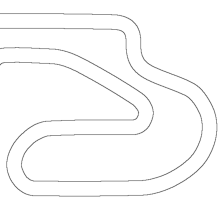
\includegraphics[interpolate=true,width=2.200000in,height=2.200000in]{contents/chapt7/figs/mu/mu_lap_1-img1.png}}%
\end{pgfscope}%
\begin{pgfscope}%
\pgfpathrectangle{\pgfqpoint{2.991542in}{0.364000in}}{\pgfqpoint{2.191917in}{2.191917in}}%
\pgfusepath{clip}%
\pgfsetbuttcap%
\pgfsetroundjoin%
\pgfsetlinewidth{1.505625pt}%
\definecolor{currentstroke}{rgb}{1.000000,0.000000,0.000000}%
\pgfsetstrokecolor{currentstroke}%
\pgfsetdash{{1.500000pt}{2.475000pt}}{0.000000pt}%
\pgfusepath{stroke}%
\end{pgfscope}%
\begin{pgfscope}%
\pgfpathrectangle{\pgfqpoint{2.991542in}{0.364000in}}{\pgfqpoint{2.191917in}{2.191917in}}%
\pgfusepath{clip}%
\pgfsetrectcap%
\pgfsetroundjoin%
\pgfsetlinewidth{1.505625pt}%
\definecolor{currentstroke}{rgb}{0.121569,0.466667,0.705882}%
\pgfsetstrokecolor{currentstroke}%
\pgfsetstrokeopacity{0.700000}%
\pgfsetdash{}{0pt}%
\pgfpathmoveto{\pgfqpoint{2.981542in}{2.325421in}}%
\pgfpathlineto{\pgfqpoint{3.044319in}{2.321712in}}%
\pgfpathlineto{\pgfqpoint{3.110013in}{2.319986in}}%
\pgfpathlineto{\pgfqpoint{3.356353in}{2.319135in}}%
\pgfpathlineto{\pgfqpoint{3.706218in}{2.317221in}}%
\pgfpathlineto{\pgfqpoint{3.762669in}{2.317491in}}%
\pgfpathlineto{\pgfqpoint{3.831322in}{2.317191in}}%
\pgfpathlineto{\pgfqpoint{3.896071in}{2.317092in}}%
\pgfpathlineto{\pgfqpoint{3.972995in}{2.317973in}}%
\pgfpathlineto{\pgfqpoint{4.065143in}{2.317526in}}%
\pgfpathlineto{\pgfqpoint{4.109361in}{2.316970in}}%
\pgfpathlineto{\pgfqpoint{4.141552in}{2.314498in}}%
\pgfpathlineto{\pgfqpoint{4.169535in}{2.310122in}}%
\pgfpathlineto{\pgfqpoint{4.193126in}{2.304166in}}%
\pgfpathlineto{\pgfqpoint{4.212223in}{2.297314in}}%
\pgfpathlineto{\pgfqpoint{4.230498in}{2.288507in}}%
\pgfpathlineto{\pgfqpoint{4.247635in}{2.277662in}}%
\pgfpathlineto{\pgfqpoint{4.263323in}{2.264814in}}%
\pgfpathlineto{\pgfqpoint{4.277266in}{2.250103in}}%
\pgfpathlineto{\pgfqpoint{4.289315in}{2.233793in}}%
\pgfpathlineto{\pgfqpoint{4.299351in}{2.216157in}}%
\pgfpathlineto{\pgfqpoint{4.309000in}{2.193800in}}%
\pgfpathlineto{\pgfqpoint{4.317993in}{2.166866in}}%
\pgfpathlineto{\pgfqpoint{4.328383in}{2.127668in}}%
\pgfpathlineto{\pgfqpoint{4.358591in}{2.005571in}}%
\pgfpathlineto{\pgfqpoint{4.368422in}{1.978954in}}%
\pgfpathlineto{\pgfqpoint{4.380434in}{1.953238in}}%
\pgfpathlineto{\pgfqpoint{4.392679in}{1.932273in}}%
\pgfpathlineto{\pgfqpoint{4.406827in}{1.912629in}}%
\pgfpathlineto{\pgfqpoint{4.422794in}{1.894671in}}%
\pgfpathlineto{\pgfqpoint{4.440409in}{1.878517in}}%
\pgfpathlineto{\pgfqpoint{4.459555in}{1.864130in}}%
\pgfpathlineto{\pgfqpoint{4.483416in}{1.849380in}}%
\pgfpathlineto{\pgfqpoint{4.511962in}{1.834583in}}%
\pgfpathlineto{\pgfqpoint{4.552403in}{1.816435in}}%
\pgfpathlineto{\pgfqpoint{4.652474in}{1.773031in}}%
\pgfpathlineto{\pgfqpoint{4.794039in}{1.702648in}}%
\pgfpathlineto{\pgfqpoint{4.836344in}{1.678499in}}%
\pgfpathlineto{\pgfqpoint{4.866853in}{1.658397in}}%
\pgfpathlineto{\pgfqpoint{4.892605in}{1.638620in}}%
\pgfpathlineto{\pgfqpoint{4.916770in}{1.616941in}}%
\pgfpathlineto{\pgfqpoint{4.939181in}{1.593494in}}%
\pgfpathlineto{\pgfqpoint{4.959734in}{1.568362in}}%
\pgfpathlineto{\pgfqpoint{4.978254in}{1.541725in}}%
\pgfpathlineto{\pgfqpoint{4.992681in}{1.517276in}}%
\pgfpathlineto{\pgfqpoint{5.005376in}{1.491871in}}%
\pgfpathlineto{\pgfqpoint{5.017734in}{1.461873in}}%
\pgfpathlineto{\pgfqpoint{5.028028in}{1.431116in}}%
\pgfpathlineto{\pgfqpoint{5.036343in}{1.399708in}}%
\pgfpathlineto{\pgfqpoint{5.042647in}{1.367841in}}%
\pgfpathlineto{\pgfqpoint{5.046703in}{1.335630in}}%
\pgfpathlineto{\pgfqpoint{5.048407in}{1.303227in}}%
\pgfpathlineto{\pgfqpoint{5.048016in}{1.270743in}}%
\pgfpathlineto{\pgfqpoint{5.045368in}{1.234309in}}%
\pgfpathlineto{\pgfqpoint{5.040873in}{1.202129in}}%
\pgfpathlineto{\pgfqpoint{5.034120in}{1.170394in}}%
\pgfpathlineto{\pgfqpoint{5.025000in}{1.139228in}}%
\pgfpathlineto{\pgfqpoint{5.013581in}{1.108844in}}%
\pgfpathlineto{\pgfqpoint{5.000178in}{1.079285in}}%
\pgfpathlineto{\pgfqpoint{4.985020in}{1.050568in}}%
\pgfpathlineto{\pgfqpoint{4.965932in}{1.019423in}}%
\pgfpathlineto{\pgfqpoint{4.938144in}{0.979394in}}%
\pgfpathlineto{\pgfqpoint{4.913730in}{0.946975in}}%
\pgfpathlineto{\pgfqpoint{4.892658in}{0.922276in}}%
\pgfpathlineto{\pgfqpoint{4.867149in}{0.896143in}}%
\pgfpathlineto{\pgfqpoint{4.802631in}{0.834449in}}%
\pgfpathlineto{\pgfqpoint{4.777632in}{0.813753in}}%
\pgfpathlineto{\pgfqpoint{4.754255in}{0.797576in}}%
\pgfpathlineto{\pgfqpoint{4.733104in}{0.785495in}}%
\pgfpathlineto{\pgfqpoint{4.703780in}{0.771597in}}%
\pgfpathlineto{\pgfqpoint{4.669929in}{0.757930in}}%
\pgfpathlineto{\pgfqpoint{4.635249in}{0.746440in}}%
\pgfpathlineto{\pgfqpoint{4.599992in}{0.737043in}}%
\pgfpathlineto{\pgfqpoint{4.552393in}{0.726841in}}%
\pgfpathlineto{\pgfqpoint{4.508330in}{0.719574in}}%
\pgfpathlineto{\pgfqpoint{4.468000in}{0.715126in}}%
\pgfpathlineto{\pgfqpoint{4.427550in}{0.713029in}}%
\pgfpathlineto{\pgfqpoint{4.383031in}{0.713267in}}%
\pgfpathlineto{\pgfqpoint{4.269640in}{0.717771in}}%
\pgfpathlineto{\pgfqpoint{4.196629in}{0.719343in}}%
\pgfpathlineto{\pgfqpoint{3.997809in}{0.719169in}}%
\pgfpathlineto{\pgfqpoint{3.831524in}{0.715111in}}%
\pgfpathlineto{\pgfqpoint{3.531203in}{0.716422in}}%
\pgfpathlineto{\pgfqpoint{3.450104in}{0.713972in}}%
\pgfpathlineto{\pgfqpoint{3.377105in}{0.712467in}}%
\pgfpathlineto{\pgfqpoint{3.340811in}{0.714017in}}%
\pgfpathlineto{\pgfqpoint{3.316934in}{0.717012in}}%
\pgfpathlineto{\pgfqpoint{3.293641in}{0.722059in}}%
\pgfpathlineto{\pgfqpoint{3.271177in}{0.729403in}}%
\pgfpathlineto{\pgfqpoint{3.249829in}{0.739086in}}%
\pgfpathlineto{\pgfqpoint{3.233125in}{0.748872in}}%
\pgfpathlineto{\pgfqpoint{3.217637in}{0.760211in}}%
\pgfpathlineto{\pgfqpoint{3.203479in}{0.772947in}}%
\pgfpathlineto{\pgfqpoint{3.190760in}{0.786941in}}%
\pgfpathlineto{\pgfqpoint{3.177508in}{0.805118in}}%
\pgfpathlineto{\pgfqpoint{3.168227in}{0.821234in}}%
\pgfpathlineto{\pgfqpoint{3.159268in}{0.841485in}}%
\pgfpathlineto{\pgfqpoint{3.152830in}{0.862468in}}%
\pgfpathlineto{\pgfqpoint{3.148852in}{0.883926in}}%
\pgfpathlineto{\pgfqpoint{3.147278in}{0.905653in}}%
\pgfpathlineto{\pgfqpoint{3.148018in}{0.927412in}}%
\pgfpathlineto{\pgfqpoint{3.150892in}{0.949392in}}%
\pgfpathlineto{\pgfqpoint{3.156795in}{0.975119in}}%
\pgfpathlineto{\pgfqpoint{3.165145in}{1.000602in}}%
\pgfpathlineto{\pgfqpoint{3.175828in}{1.025582in}}%
\pgfpathlineto{\pgfqpoint{3.188665in}{1.049827in}}%
\pgfpathlineto{\pgfqpoint{3.203494in}{1.073172in}}%
\pgfpathlineto{\pgfqpoint{3.220111in}{1.095500in}}%
\pgfpathlineto{\pgfqpoint{3.241080in}{1.119644in}}%
\pgfpathlineto{\pgfqpoint{3.263808in}{1.142262in}}%
\pgfpathlineto{\pgfqpoint{3.313935in}{1.188725in}}%
\pgfpathlineto{\pgfqpoint{3.338712in}{1.208573in}}%
\pgfpathlineto{\pgfqpoint{3.361856in}{1.223948in}}%
\pgfpathlineto{\pgfqpoint{3.382922in}{1.235283in}}%
\pgfpathlineto{\pgfqpoint{3.404985in}{1.244671in}}%
\pgfpathlineto{\pgfqpoint{3.427825in}{1.252018in}}%
\pgfpathlineto{\pgfqpoint{3.458983in}{1.259812in}}%
\pgfpathlineto{\pgfqpoint{3.506406in}{1.269204in}}%
\pgfpathlineto{\pgfqpoint{3.558276in}{1.277198in}}%
\pgfpathlineto{\pgfqpoint{3.682647in}{1.293546in}}%
\pgfpathlineto{\pgfqpoint{3.741990in}{1.299094in}}%
\pgfpathlineto{\pgfqpoint{3.796283in}{1.301975in}}%
\pgfpathlineto{\pgfqpoint{4.096257in}{1.311223in}}%
\pgfpathlineto{\pgfqpoint{4.214458in}{1.315402in}}%
\pgfpathlineto{\pgfqpoint{4.263101in}{1.318854in}}%
\pgfpathlineto{\pgfqpoint{4.297085in}{1.323330in}}%
\pgfpathlineto{\pgfqpoint{4.319654in}{1.328182in}}%
\pgfpathlineto{\pgfqpoint{4.341643in}{1.335271in}}%
\pgfpathlineto{\pgfqpoint{4.358984in}{1.343266in}}%
\pgfpathlineto{\pgfqpoint{4.374987in}{1.353367in}}%
\pgfpathlineto{\pgfqpoint{4.386490in}{1.363017in}}%
\pgfpathlineto{\pgfqpoint{4.396589in}{1.373977in}}%
\pgfpathlineto{\pgfqpoint{4.405081in}{1.386085in}}%
\pgfpathlineto{\pgfqpoint{4.411838in}{1.399134in}}%
\pgfpathlineto{\pgfqpoint{4.416762in}{1.412892in}}%
\pgfpathlineto{\pgfqpoint{4.419846in}{1.427099in}}%
\pgfpathlineto{\pgfqpoint{4.421099in}{1.441509in}}%
\pgfpathlineto{\pgfqpoint{4.420154in}{1.459543in}}%
\pgfpathlineto{\pgfqpoint{4.416551in}{1.477255in}}%
\pgfpathlineto{\pgfqpoint{4.410500in}{1.494520in}}%
\pgfpathlineto{\pgfqpoint{4.402245in}{1.511138in}}%
\pgfpathlineto{\pgfqpoint{4.392096in}{1.526889in}}%
\pgfpathlineto{\pgfqpoint{4.377830in}{1.544473in}}%
\pgfpathlineto{\pgfqpoint{4.361680in}{1.560529in}}%
\pgfpathlineto{\pgfqpoint{4.340987in}{1.577542in}}%
\pgfpathlineto{\pgfqpoint{4.247345in}{1.647940in}}%
\pgfpathlineto{\pgfqpoint{4.197726in}{1.680417in}}%
\pgfpathlineto{\pgfqpoint{4.158262in}{1.707626in}}%
\pgfpathlineto{\pgfqpoint{4.122110in}{1.732536in}}%
\pgfpathlineto{\pgfqpoint{4.098095in}{1.746628in}}%
\pgfpathlineto{\pgfqpoint{4.065905in}{1.762382in}}%
\pgfpathlineto{\pgfqpoint{4.011924in}{1.788960in}}%
\pgfpathlineto{\pgfqpoint{3.976885in}{1.809078in}}%
\pgfpathlineto{\pgfqpoint{3.935250in}{1.832846in}}%
\pgfpathlineto{\pgfqpoint{3.906826in}{1.846678in}}%
\pgfpathlineto{\pgfqpoint{3.786963in}{1.899394in}}%
\pgfpathlineto{\pgfqpoint{3.746655in}{1.913979in}}%
\pgfpathlineto{\pgfqpoint{3.698750in}{1.928783in}}%
\pgfpathlineto{\pgfqpoint{3.650525in}{1.941311in}}%
\pgfpathlineto{\pgfqpoint{3.597303in}{1.952529in}}%
\pgfpathlineto{\pgfqpoint{3.535081in}{1.963406in}}%
\pgfpathlineto{\pgfqpoint{3.479637in}{1.971096in}}%
\pgfpathlineto{\pgfqpoint{3.423597in}{1.976294in}}%
\pgfpathlineto{\pgfqpoint{3.346968in}{1.980854in}}%
\pgfpathlineto{\pgfqpoint{3.261877in}{1.983960in}}%
\pgfpathlineto{\pgfqpoint{3.193127in}{1.984134in}}%
\pgfpathlineto{\pgfqpoint{3.125899in}{1.981945in}}%
\pgfpathlineto{\pgfqpoint{3.072041in}{1.978229in}}%
\pgfpathlineto{\pgfqpoint{3.041864in}{1.974269in}}%
\pgfpathlineto{\pgfqpoint{3.019631in}{1.969346in}}%
\pgfpathlineto{\pgfqpoint{3.001649in}{1.963472in}}%
\pgfpathlineto{\pgfqpoint{2.984353in}{1.955719in}}%
\pgfpathlineto{\pgfqpoint{2.981542in}{1.954227in}}%
\pgfpathlineto{\pgfqpoint{2.981542in}{1.954227in}}%
\pgfusepath{stroke}%
\end{pgfscope}%
\begin{pgfscope}%
\pgfpathrectangle{\pgfqpoint{2.991542in}{0.364000in}}{\pgfqpoint{2.191917in}{2.191917in}}%
\pgfusepath{clip}%
\pgfsetbuttcap%
\pgfsetroundjoin%
\pgfsetlinewidth{1.505625pt}%
\definecolor{currentstroke}{rgb}{1.000000,0.498039,0.054902}%
\pgfsetstrokecolor{currentstroke}%
\pgfsetstrokeopacity{0.700000}%
\pgfsetdash{{5.550000pt}{2.400000pt}}{0.000000pt}%
\pgfpathmoveto{\pgfqpoint{2.981542in}{2.331390in}}%
\pgfpathlineto{\pgfqpoint{3.069103in}{2.324946in}}%
\pgfpathlineto{\pgfqpoint{3.138151in}{2.322094in}}%
\pgfpathlineto{\pgfqpoint{3.406325in}{2.316778in}}%
\pgfpathlineto{\pgfqpoint{3.517295in}{2.318186in}}%
\pgfpathlineto{\pgfqpoint{3.621034in}{2.316603in}}%
\pgfpathlineto{\pgfqpoint{3.713467in}{2.316470in}}%
\pgfpathlineto{\pgfqpoint{3.789714in}{2.316397in}}%
\pgfpathlineto{\pgfqpoint{3.882494in}{2.316321in}}%
\pgfpathlineto{\pgfqpoint{3.951225in}{2.316992in}}%
\pgfpathlineto{\pgfqpoint{4.019868in}{2.317049in}}%
\pgfpathlineto{\pgfqpoint{4.159843in}{2.313715in}}%
\pgfpathlineto{\pgfqpoint{4.187467in}{2.309707in}}%
\pgfpathlineto{\pgfqpoint{4.210735in}{2.303848in}}%
\pgfpathlineto{\pgfqpoint{4.229572in}{2.296993in}}%
\pgfpathlineto{\pgfqpoint{4.247662in}{2.288239in}}%
\pgfpathlineto{\pgfqpoint{4.264716in}{2.277557in}}%
\pgfpathlineto{\pgfqpoint{4.280469in}{2.264956in}}%
\pgfpathlineto{\pgfqpoint{4.294656in}{2.250615in}}%
\pgfpathlineto{\pgfqpoint{4.307063in}{2.234716in}}%
\pgfpathlineto{\pgfqpoint{4.317634in}{2.217548in}}%
\pgfpathlineto{\pgfqpoint{4.328042in}{2.195638in}}%
\pgfpathlineto{\pgfqpoint{4.336470in}{2.172858in}}%
\pgfpathlineto{\pgfqpoint{4.345472in}{2.141713in}}%
\pgfpathlineto{\pgfqpoint{4.355419in}{2.098200in}}%
\pgfpathlineto{\pgfqpoint{4.379958in}{1.983318in}}%
\pgfpathlineto{\pgfqpoint{4.388620in}{1.956267in}}%
\pgfpathlineto{\pgfqpoint{4.397825in}{1.933753in}}%
\pgfpathlineto{\pgfqpoint{4.408933in}{1.912140in}}%
\pgfpathlineto{\pgfqpoint{4.422091in}{1.891752in}}%
\pgfpathlineto{\pgfqpoint{4.434550in}{1.876012in}}%
\pgfpathlineto{\pgfqpoint{4.448357in}{1.861530in}}%
\pgfpathlineto{\pgfqpoint{4.466657in}{1.845878in}}%
\pgfpathlineto{\pgfqpoint{4.486520in}{1.832159in}}%
\pgfpathlineto{\pgfqpoint{4.511052in}{1.818247in}}%
\pgfpathlineto{\pgfqpoint{4.540279in}{1.804560in}}%
\pgfpathlineto{\pgfqpoint{4.774783in}{1.703926in}}%
\pgfpathlineto{\pgfqpoint{4.817846in}{1.681357in}}%
\pgfpathlineto{\pgfqpoint{4.852688in}{1.660572in}}%
\pgfpathlineto{\pgfqpoint{4.879492in}{1.642243in}}%
\pgfpathlineto{\pgfqpoint{4.904967in}{1.622113in}}%
\pgfpathlineto{\pgfqpoint{4.928992in}{1.600273in}}%
\pgfpathlineto{\pgfqpoint{4.951466in}{1.576827in}}%
\pgfpathlineto{\pgfqpoint{4.972265in}{1.551935in}}%
\pgfpathlineto{\pgfqpoint{4.991231in}{1.525626in}}%
\pgfpathlineto{\pgfqpoint{5.008201in}{1.497975in}}%
\pgfpathlineto{\pgfqpoint{5.023051in}{1.469112in}}%
\pgfpathlineto{\pgfqpoint{5.035691in}{1.439215in}}%
\pgfpathlineto{\pgfqpoint{5.046053in}{1.408476in}}%
\pgfpathlineto{\pgfqpoint{5.054087in}{1.377055in}}%
\pgfpathlineto{\pgfqpoint{5.059761in}{1.345088in}}%
\pgfpathlineto{\pgfqpoint{5.063214in}{1.312791in}}%
\pgfpathlineto{\pgfqpoint{5.064583in}{1.276315in}}%
\pgfpathlineto{\pgfqpoint{5.063539in}{1.239850in}}%
\pgfpathlineto{\pgfqpoint{5.059993in}{1.199396in}}%
\pgfpathlineto{\pgfqpoint{5.053340in}{1.151140in}}%
\pgfpathlineto{\pgfqpoint{5.045711in}{1.111285in}}%
\pgfpathlineto{\pgfqpoint{5.037484in}{1.079901in}}%
\pgfpathlineto{\pgfqpoint{5.028259in}{1.053037in}}%
\pgfpathlineto{\pgfqpoint{5.016907in}{1.026993in}}%
\pgfpathlineto{\pgfqpoint{5.003501in}{1.001952in}}%
\pgfpathlineto{\pgfqpoint{4.988193in}{0.978026in}}%
\pgfpathlineto{\pgfqpoint{4.971196in}{0.955309in}}%
\pgfpathlineto{\pgfqpoint{4.952594in}{0.933867in}}%
\pgfpathlineto{\pgfqpoint{4.926724in}{0.908074in}}%
\pgfpathlineto{\pgfqpoint{4.887611in}{0.872734in}}%
\pgfpathlineto{\pgfqpoint{4.853457in}{0.843991in}}%
\pgfpathlineto{\pgfqpoint{4.824071in}{0.822307in}}%
\pgfpathlineto{\pgfqpoint{4.789967in}{0.800393in}}%
\pgfpathlineto{\pgfqpoint{4.744396in}{0.773869in}}%
\pgfpathlineto{\pgfqpoint{4.715445in}{0.759130in}}%
\pgfpathlineto{\pgfqpoint{4.681906in}{0.744763in}}%
\pgfpathlineto{\pgfqpoint{4.651236in}{0.734111in}}%
\pgfpathlineto{\pgfqpoint{4.616023in}{0.724410in}}%
\pgfpathlineto{\pgfqpoint{4.580314in}{0.716826in}}%
\pgfpathlineto{\pgfqpoint{4.540281in}{0.710675in}}%
\pgfpathlineto{\pgfqpoint{4.499982in}{0.706797in}}%
\pgfpathlineto{\pgfqpoint{4.459435in}{0.705161in}}%
\pgfpathlineto{\pgfqpoint{4.414765in}{0.705805in}}%
\pgfpathlineto{\pgfqpoint{4.362104in}{0.709034in}}%
\pgfpathlineto{\pgfqpoint{4.188034in}{0.721883in}}%
\pgfpathlineto{\pgfqpoint{4.119085in}{0.723844in}}%
\pgfpathlineto{\pgfqpoint{4.025725in}{0.724048in}}%
\pgfpathlineto{\pgfqpoint{3.948612in}{0.721948in}}%
\pgfpathlineto{\pgfqpoint{3.749910in}{0.714235in}}%
\pgfpathlineto{\pgfqpoint{3.607896in}{0.713065in}}%
\pgfpathlineto{\pgfqpoint{3.324550in}{0.718631in}}%
\pgfpathlineto{\pgfqpoint{3.297059in}{0.722464in}}%
\pgfpathlineto{\pgfqpoint{3.274093in}{0.727822in}}%
\pgfpathlineto{\pgfqpoint{3.252017in}{0.735407in}}%
\pgfpathlineto{\pgfqpoint{3.234563in}{0.743523in}}%
\pgfpathlineto{\pgfqpoint{3.218190in}{0.753291in}}%
\pgfpathlineto{\pgfqpoint{3.203091in}{0.764651in}}%
\pgfpathlineto{\pgfqpoint{3.189398in}{0.777427in}}%
\pgfpathlineto{\pgfqpoint{3.177208in}{0.791443in}}%
\pgfpathlineto{\pgfqpoint{3.166588in}{0.806500in}}%
\pgfpathlineto{\pgfqpoint{3.157635in}{0.822441in}}%
\pgfpathlineto{\pgfqpoint{3.149060in}{0.842479in}}%
\pgfpathlineto{\pgfqpoint{3.142838in}{0.863258in}}%
\pgfpathlineto{\pgfqpoint{3.138911in}{0.884546in}}%
\pgfpathlineto{\pgfqpoint{3.137134in}{0.906122in}}%
\pgfpathlineto{\pgfqpoint{3.137441in}{0.927859in}}%
\pgfpathlineto{\pgfqpoint{3.139772in}{0.949924in}}%
\pgfpathlineto{\pgfqpoint{3.144926in}{0.975839in}}%
\pgfpathlineto{\pgfqpoint{3.152611in}{1.001545in}}%
\pgfpathlineto{\pgfqpoint{3.162684in}{1.026766in}}%
\pgfpathlineto{\pgfqpoint{3.175006in}{1.051223in}}%
\pgfpathlineto{\pgfqpoint{3.189457in}{1.074733in}}%
\pgfpathlineto{\pgfqpoint{3.205819in}{1.097138in}}%
\pgfpathlineto{\pgfqpoint{3.226533in}{1.121326in}}%
\pgfpathlineto{\pgfqpoint{3.256901in}{1.153173in}}%
\pgfpathlineto{\pgfqpoint{3.283378in}{1.177677in}}%
\pgfpathlineto{\pgfqpoint{3.308458in}{1.197799in}}%
\pgfpathlineto{\pgfqpoint{3.331775in}{1.213657in}}%
\pgfpathlineto{\pgfqpoint{3.356306in}{1.227728in}}%
\pgfpathlineto{\pgfqpoint{3.381921in}{1.239912in}}%
\pgfpathlineto{\pgfqpoint{3.408427in}{1.250119in}}%
\pgfpathlineto{\pgfqpoint{3.439439in}{1.259780in}}%
\pgfpathlineto{\pgfqpoint{3.471008in}{1.267389in}}%
\pgfpathlineto{\pgfqpoint{3.507028in}{1.273597in}}%
\pgfpathlineto{\pgfqpoint{3.567420in}{1.281176in}}%
\pgfpathlineto{\pgfqpoint{3.715738in}{1.297898in}}%
\pgfpathlineto{\pgfqpoint{3.787850in}{1.301667in}}%
\pgfpathlineto{\pgfqpoint{3.936481in}{1.306293in}}%
\pgfpathlineto{\pgfqpoint{4.137788in}{1.311340in}}%
\pgfpathlineto{\pgfqpoint{4.215484in}{1.314384in}}%
\pgfpathlineto{\pgfqpoint{4.268066in}{1.318295in}}%
\pgfpathlineto{\pgfqpoint{4.302167in}{1.322824in}}%
\pgfpathlineto{\pgfqpoint{4.328566in}{1.328480in}}%
\pgfpathlineto{\pgfqpoint{4.350570in}{1.335433in}}%
\pgfpathlineto{\pgfqpoint{4.368046in}{1.343082in}}%
\pgfpathlineto{\pgfqpoint{4.384324in}{1.352640in}}%
\pgfpathlineto{\pgfqpoint{4.399001in}{1.364183in}}%
\pgfpathlineto{\pgfqpoint{4.409330in}{1.374820in}}%
\pgfpathlineto{\pgfqpoint{4.418193in}{1.386589in}}%
\pgfpathlineto{\pgfqpoint{4.425436in}{1.399317in}}%
\pgfpathlineto{\pgfqpoint{4.430987in}{1.412791in}}%
\pgfpathlineto{\pgfqpoint{4.434786in}{1.426773in}}%
\pgfpathlineto{\pgfqpoint{4.437017in}{1.444433in}}%
\pgfpathlineto{\pgfqpoint{4.436797in}{1.458438in}}%
\pgfpathlineto{\pgfqpoint{4.434056in}{1.475863in}}%
\pgfpathlineto{\pgfqpoint{4.428812in}{1.493097in}}%
\pgfpathlineto{\pgfqpoint{4.421447in}{1.509856in}}%
\pgfpathlineto{\pgfqpoint{4.412248in}{1.525925in}}%
\pgfpathlineto{\pgfqpoint{4.399127in}{1.544109in}}%
\pgfpathlineto{\pgfqpoint{4.384047in}{1.560993in}}%
\pgfpathlineto{\pgfqpoint{4.367270in}{1.576423in}}%
\pgfpathlineto{\pgfqpoint{4.349052in}{1.590329in}}%
\pgfpathlineto{\pgfqpoint{4.316576in}{1.611660in}}%
\pgfpathlineto{\pgfqpoint{4.243381in}{1.658710in}}%
\pgfpathlineto{\pgfqpoint{4.169941in}{1.707373in}}%
\pgfpathlineto{\pgfqpoint{4.117850in}{1.737978in}}%
\pgfpathlineto{\pgfqpoint{3.981217in}{1.815609in}}%
\pgfpathlineto{\pgfqpoint{3.926332in}{1.840340in}}%
\pgfpathlineto{\pgfqpoint{3.878745in}{1.862516in}}%
\pgfpathlineto{\pgfqpoint{3.785365in}{1.908151in}}%
\pgfpathlineto{\pgfqpoint{3.752187in}{1.920909in}}%
\pgfpathlineto{\pgfqpoint{3.718550in}{1.931460in}}%
\pgfpathlineto{\pgfqpoint{3.657692in}{1.947712in}}%
\pgfpathlineto{\pgfqpoint{3.604081in}{1.960278in}}%
\pgfpathlineto{\pgfqpoint{3.565655in}{1.966906in}}%
\pgfpathlineto{\pgfqpoint{3.522632in}{1.971887in}}%
\pgfpathlineto{\pgfqpoint{3.447141in}{1.977991in}}%
\pgfpathlineto{\pgfqpoint{3.350698in}{1.983659in}}%
\pgfpathlineto{\pgfqpoint{3.269767in}{1.986450in}}%
\pgfpathlineto{\pgfqpoint{3.200991in}{1.986699in}}%
\pgfpathlineto{\pgfqpoint{3.133265in}{1.984791in}}%
\pgfpathlineto{\pgfqpoint{3.074939in}{1.981107in}}%
\pgfpathlineto{\pgfqpoint{3.040670in}{1.976999in}}%
\pgfpathlineto{\pgfqpoint{3.014510in}{1.971631in}}%
\pgfpathlineto{\pgfqpoint{2.992735in}{1.964855in}}%
\pgfpathlineto{\pgfqpoint{2.981542in}{1.960305in}}%
\pgfpathlineto{\pgfqpoint{2.981542in}{1.960305in}}%
\pgfusepath{stroke}%
\end{pgfscope}%
\begin{pgfscope}%
\pgfpathrectangle{\pgfqpoint{2.991542in}{0.364000in}}{\pgfqpoint{2.191917in}{2.191917in}}%
\pgfusepath{clip}%
\pgfsetbuttcap%
\pgfsetroundjoin%
\pgfsetlinewidth{1.505625pt}%
\definecolor{currentstroke}{rgb}{0.172549,0.627451,0.172549}%
\pgfsetstrokecolor{currentstroke}%
\pgfsetstrokeopacity{0.700000}%
\pgfsetdash{{5.550000pt}{2.400000pt}}{0.000000pt}%
\pgfpathmoveto{\pgfqpoint{2.981542in}{2.320134in}}%
\pgfpathlineto{\pgfqpoint{3.055142in}{2.319141in}}%
\pgfpathlineto{\pgfqpoint{3.261531in}{2.317103in}}%
\pgfpathlineto{\pgfqpoint{3.409974in}{2.316846in}}%
\pgfpathlineto{\pgfqpoint{3.533121in}{2.318979in}}%
\pgfpathlineto{\pgfqpoint{3.660977in}{2.320214in}}%
\pgfpathlineto{\pgfqpoint{3.749081in}{2.319390in}}%
\pgfpathlineto{\pgfqpoint{3.821169in}{2.319582in}}%
\pgfpathlineto{\pgfqpoint{3.897747in}{2.319485in}}%
\pgfpathlineto{\pgfqpoint{3.990475in}{2.319085in}}%
\pgfpathlineto{\pgfqpoint{4.091136in}{2.320423in}}%
\pgfpathlineto{\pgfqpoint{4.131594in}{2.318287in}}%
\pgfpathlineto{\pgfqpoint{4.167903in}{2.314212in}}%
\pgfpathlineto{\pgfqpoint{4.195848in}{2.309101in}}%
\pgfpathlineto{\pgfqpoint{4.223242in}{2.301746in}}%
\pgfpathlineto{\pgfqpoint{4.246007in}{2.293222in}}%
\pgfpathlineto{\pgfqpoint{4.264222in}{2.284291in}}%
\pgfpathlineto{\pgfqpoint{4.281484in}{2.273599in}}%
\pgfpathlineto{\pgfqpoint{4.297489in}{2.261136in}}%
\pgfpathlineto{\pgfqpoint{4.312000in}{2.246967in}}%
\pgfpathlineto{\pgfqpoint{4.324800in}{2.231230in}}%
\pgfpathlineto{\pgfqpoint{4.335809in}{2.214177in}}%
\pgfpathlineto{\pgfqpoint{4.345074in}{2.196128in}}%
\pgfpathlineto{\pgfqpoint{4.354100in}{2.173531in}}%
\pgfpathlineto{\pgfqpoint{4.361167in}{2.150253in}}%
\pgfpathlineto{\pgfqpoint{4.368296in}{2.118581in}}%
\pgfpathlineto{\pgfqpoint{4.374806in}{2.078539in}}%
\pgfpathlineto{\pgfqpoint{4.390379in}{1.974247in}}%
\pgfpathlineto{\pgfqpoint{4.397176in}{1.946734in}}%
\pgfpathlineto{\pgfqpoint{4.406248in}{1.919849in}}%
\pgfpathlineto{\pgfqpoint{4.416106in}{1.897691in}}%
\pgfpathlineto{\pgfqpoint{4.428043in}{1.876699in}}%
\pgfpathlineto{\pgfqpoint{4.442057in}{1.857224in}}%
\pgfpathlineto{\pgfqpoint{4.455320in}{1.842311in}}%
\pgfpathlineto{\pgfqpoint{4.469946in}{1.828653in}}%
\pgfpathlineto{\pgfqpoint{4.489029in}{1.814008in}}%
\pgfpathlineto{\pgfqpoint{4.509389in}{1.801103in}}%
\pgfpathlineto{\pgfqpoint{4.534301in}{1.787965in}}%
\pgfpathlineto{\pgfqpoint{4.567434in}{1.773249in}}%
\pgfpathlineto{\pgfqpoint{4.627477in}{1.749567in}}%
\pgfpathlineto{\pgfqpoint{4.707433in}{1.720283in}}%
\pgfpathlineto{\pgfqpoint{4.779579in}{1.693111in}}%
\pgfpathlineto{\pgfqpoint{4.820546in}{1.675334in}}%
\pgfpathlineto{\pgfqpoint{4.853158in}{1.658977in}}%
\pgfpathlineto{\pgfqpoint{4.881176in}{1.642607in}}%
\pgfpathlineto{\pgfqpoint{4.907894in}{1.624272in}}%
\pgfpathlineto{\pgfqpoint{4.930018in}{1.606475in}}%
\pgfpathlineto{\pgfqpoint{4.950840in}{1.587135in}}%
\pgfpathlineto{\pgfqpoint{4.970245in}{1.566396in}}%
\pgfpathlineto{\pgfqpoint{4.990719in}{1.541215in}}%
\pgfpathlineto{\pgfqpoint{5.009431in}{1.514650in}}%
\pgfpathlineto{\pgfqpoint{5.028496in}{1.483482in}}%
\pgfpathlineto{\pgfqpoint{5.045485in}{1.451151in}}%
\pgfpathlineto{\pgfqpoint{5.060495in}{1.417865in}}%
\pgfpathlineto{\pgfqpoint{5.073481in}{1.383738in}}%
\pgfpathlineto{\pgfqpoint{5.083132in}{1.352727in}}%
\pgfpathlineto{\pgfqpoint{5.090668in}{1.321154in}}%
\pgfpathlineto{\pgfqpoint{5.095811in}{1.289088in}}%
\pgfpathlineto{\pgfqpoint{5.098255in}{1.260834in}}%
\pgfpathlineto{\pgfqpoint{5.098742in}{1.232435in}}%
\pgfpathlineto{\pgfqpoint{5.096899in}{1.200015in}}%
\pgfpathlineto{\pgfqpoint{5.093209in}{1.171845in}}%
\pgfpathlineto{\pgfqpoint{5.087541in}{1.144030in}}%
\pgfpathlineto{\pgfqpoint{5.079935in}{1.116678in}}%
\pgfpathlineto{\pgfqpoint{5.070445in}{1.089946in}}%
\pgfpathlineto{\pgfqpoint{5.059070in}{1.063947in}}%
\pgfpathlineto{\pgfqpoint{5.044001in}{1.035186in}}%
\pgfpathlineto{\pgfqpoint{5.026873in}{1.007632in}}%
\pgfpathlineto{\pgfqpoint{5.005513in}{0.978121in}}%
\pgfpathlineto{\pgfqpoint{4.979993in}{0.946672in}}%
\pgfpathlineto{\pgfqpoint{4.947603in}{0.910342in}}%
\pgfpathlineto{\pgfqpoint{4.919029in}{0.881583in}}%
\pgfpathlineto{\pgfqpoint{4.894732in}{0.860042in}}%
\pgfpathlineto{\pgfqpoint{4.869032in}{0.840187in}}%
\pgfpathlineto{\pgfqpoint{4.838852in}{0.819617in}}%
\pgfpathlineto{\pgfqpoint{4.807423in}{0.800974in}}%
\pgfpathlineto{\pgfqpoint{4.774962in}{0.784123in}}%
\pgfpathlineto{\pgfqpoint{4.741557in}{0.769337in}}%
\pgfpathlineto{\pgfqpoint{4.711080in}{0.758151in}}%
\pgfpathlineto{\pgfqpoint{4.676032in}{0.747871in}}%
\pgfpathlineto{\pgfqpoint{4.640412in}{0.739829in}}%
\pgfpathlineto{\pgfqpoint{4.596386in}{0.732294in}}%
\pgfpathlineto{\pgfqpoint{4.536015in}{0.724477in}}%
\pgfpathlineto{\pgfqpoint{4.467352in}{0.717828in}}%
\pgfpathlineto{\pgfqpoint{4.410688in}{0.714719in}}%
\pgfpathlineto{\pgfqpoint{4.353942in}{0.713972in}}%
\pgfpathlineto{\pgfqpoint{4.284957in}{0.715512in}}%
\pgfpathlineto{\pgfqpoint{4.126717in}{0.719802in}}%
\pgfpathlineto{\pgfqpoint{3.984739in}{0.720958in}}%
\pgfpathlineto{\pgfqpoint{3.899586in}{0.719240in}}%
\pgfpathlineto{\pgfqpoint{3.769845in}{0.716569in}}%
\pgfpathlineto{\pgfqpoint{3.429257in}{0.714815in}}%
\pgfpathlineto{\pgfqpoint{3.356572in}{0.715544in}}%
\pgfpathlineto{\pgfqpoint{3.316535in}{0.718166in}}%
\pgfpathlineto{\pgfqpoint{3.289049in}{0.721970in}}%
\pgfpathlineto{\pgfqpoint{3.262365in}{0.728038in}}%
\pgfpathlineto{\pgfqpoint{3.240425in}{0.735372in}}%
\pgfpathlineto{\pgfqpoint{3.219615in}{0.744869in}}%
\pgfpathlineto{\pgfqpoint{3.203352in}{0.754467in}}%
\pgfpathlineto{\pgfqpoint{3.188245in}{0.765559in}}%
\pgfpathlineto{\pgfqpoint{3.174451in}{0.778038in}}%
\pgfpathlineto{\pgfqpoint{3.162110in}{0.791777in}}%
\pgfpathlineto{\pgfqpoint{3.149300in}{0.809680in}}%
\pgfpathlineto{\pgfqpoint{3.138743in}{0.828836in}}%
\pgfpathlineto{\pgfqpoint{3.130433in}{0.848995in}}%
\pgfpathlineto{\pgfqpoint{3.124346in}{0.869943in}}%
\pgfpathlineto{\pgfqpoint{3.120403in}{0.891430in}}%
\pgfpathlineto{\pgfqpoint{3.118567in}{0.913198in}}%
\pgfpathlineto{\pgfqpoint{3.118773in}{0.935055in}}%
\pgfpathlineto{\pgfqpoint{3.120977in}{0.956819in}}%
\pgfpathlineto{\pgfqpoint{3.125191in}{0.978476in}}%
\pgfpathlineto{\pgfqpoint{3.132565in}{1.003642in}}%
\pgfpathlineto{\pgfqpoint{3.142392in}{1.028433in}}%
\pgfpathlineto{\pgfqpoint{3.154472in}{1.052508in}}%
\pgfpathlineto{\pgfqpoint{3.168607in}{1.075730in}}%
\pgfpathlineto{\pgfqpoint{3.184684in}{1.098005in}}%
\pgfpathlineto{\pgfqpoint{3.207357in}{1.124920in}}%
\pgfpathlineto{\pgfqpoint{3.231580in}{1.150310in}}%
\pgfpathlineto{\pgfqpoint{3.257656in}{1.174330in}}%
\pgfpathlineto{\pgfqpoint{3.282360in}{1.194289in}}%
\pgfpathlineto{\pgfqpoint{3.308437in}{1.212629in}}%
\pgfpathlineto{\pgfqpoint{3.335856in}{1.229121in}}%
\pgfpathlineto{\pgfqpoint{3.364563in}{1.243543in}}%
\pgfpathlineto{\pgfqpoint{3.394331in}{1.255762in}}%
\pgfpathlineto{\pgfqpoint{3.424935in}{1.265827in}}%
\pgfpathlineto{\pgfqpoint{3.452357in}{1.272591in}}%
\pgfpathlineto{\pgfqpoint{3.488160in}{1.278844in}}%
\pgfpathlineto{\pgfqpoint{3.532446in}{1.284075in}}%
\pgfpathlineto{\pgfqpoint{3.693110in}{1.298993in}}%
\pgfpathlineto{\pgfqpoint{3.752933in}{1.302200in}}%
\pgfpathlineto{\pgfqpoint{3.877495in}{1.305787in}}%
\pgfpathlineto{\pgfqpoint{4.018054in}{1.308238in}}%
\pgfpathlineto{\pgfqpoint{4.149045in}{1.312014in}}%
\pgfpathlineto{\pgfqpoint{4.261985in}{1.316075in}}%
\pgfpathlineto{\pgfqpoint{4.300370in}{1.319615in}}%
\pgfpathlineto{\pgfqpoint{4.330818in}{1.324617in}}%
\pgfpathlineto{\pgfqpoint{4.352965in}{1.330316in}}%
\pgfpathlineto{\pgfqpoint{4.374109in}{1.338195in}}%
\pgfpathlineto{\pgfqpoint{4.390665in}{1.346698in}}%
\pgfpathlineto{\pgfqpoint{4.405949in}{1.357091in}}%
\pgfpathlineto{\pgfqpoint{4.419603in}{1.369332in}}%
\pgfpathlineto{\pgfqpoint{4.431297in}{1.383279in}}%
\pgfpathlineto{\pgfqpoint{4.440771in}{1.398695in}}%
\pgfpathlineto{\pgfqpoint{4.447855in}{1.415231in}}%
\pgfpathlineto{\pgfqpoint{4.452463in}{1.432550in}}%
\pgfpathlineto{\pgfqpoint{4.454630in}{1.450297in}}%
\pgfpathlineto{\pgfqpoint{4.454394in}{1.468091in}}%
\pgfpathlineto{\pgfqpoint{4.451898in}{1.485564in}}%
\pgfpathlineto{\pgfqpoint{4.447237in}{1.502614in}}%
\pgfpathlineto{\pgfqpoint{4.440542in}{1.519275in}}%
\pgfpathlineto{\pgfqpoint{4.430098in}{1.538513in}}%
\pgfpathlineto{\pgfqpoint{4.417468in}{1.556688in}}%
\pgfpathlineto{\pgfqpoint{4.402840in}{1.573807in}}%
\pgfpathlineto{\pgfqpoint{4.386469in}{1.589704in}}%
\pgfpathlineto{\pgfqpoint{4.365722in}{1.606889in}}%
\pgfpathlineto{\pgfqpoint{4.340537in}{1.625049in}}%
\pgfpathlineto{\pgfqpoint{4.307456in}{1.646151in}}%
\pgfpathlineto{\pgfqpoint{4.262822in}{1.671757in}}%
\pgfpathlineto{\pgfqpoint{4.184800in}{1.713161in}}%
\pgfpathlineto{\pgfqpoint{4.095759in}{1.761132in}}%
\pgfpathlineto{\pgfqpoint{3.978064in}{1.824985in}}%
\pgfpathlineto{\pgfqpoint{3.933676in}{1.844903in}}%
\pgfpathlineto{\pgfqpoint{3.770885in}{1.912704in}}%
\pgfpathlineto{\pgfqpoint{3.726413in}{1.927968in}}%
\pgfpathlineto{\pgfqpoint{3.654630in}{1.950251in}}%
\pgfpathlineto{\pgfqpoint{3.609182in}{1.962221in}}%
\pgfpathlineto{\pgfqpoint{3.570772in}{1.970038in}}%
\pgfpathlineto{\pgfqpoint{3.527691in}{1.976536in}}%
\pgfpathlineto{\pgfqpoint{3.472126in}{1.982488in}}%
\pgfpathlineto{\pgfqpoint{3.404009in}{1.987442in}}%
\pgfpathlineto{\pgfqpoint{3.327278in}{1.990842in}}%
\pgfpathlineto{\pgfqpoint{3.266424in}{1.991579in}}%
\pgfpathlineto{\pgfqpoint{3.201535in}{1.990104in}}%
\pgfpathlineto{\pgfqpoint{3.113644in}{1.985976in}}%
\pgfpathlineto{\pgfqpoint{3.055529in}{1.981576in}}%
\pgfpathlineto{\pgfqpoint{3.021415in}{1.976857in}}%
\pgfpathlineto{\pgfqpoint{2.995434in}{1.970991in}}%
\pgfpathlineto{\pgfqpoint{2.981542in}{1.966664in}}%
\pgfpathlineto{\pgfqpoint{2.981542in}{1.966664in}}%
\pgfusepath{stroke}%
\end{pgfscope}%
\begin{pgfscope}%
\definecolor{textcolor}{rgb}{0.000000,0.000000,0.000000}%
\pgfsetstrokecolor{textcolor}%
\pgfsetfillcolor{textcolor}%
\pgftext[x=4.087500in,y=2.639250in,,base]{\color{textcolor}\rmfamily\fontsize{12.000000}{14.400000}\selectfont Partial end-to-end}%
\end{pgfscope}%
\begin{pgfscope}%
\pgfsetbuttcap%
\pgfsetmiterjoin%
\definecolor{currentfill}{rgb}{1.000000,1.000000,1.000000}%
\pgfsetfillcolor{currentfill}%
\pgfsetfillopacity{0.800000}%
\pgfsetlinewidth{1.003750pt}%
\definecolor{currentstroke}{rgb}{0.800000,0.800000,0.800000}%
\pgfsetstrokecolor{currentstroke}%
\pgfsetstrokeopacity{0.800000}%
\pgfsetdash{}{0pt}%
\pgfpathmoveto{\pgfqpoint{0.670702in}{0.069444in}}%
\pgfpathlineto{\pgfqpoint{4.829298in}{0.069444in}}%
\pgfpathquadraticcurveto{\pgfqpoint{4.857076in}{0.069444in}}{\pgfqpoint{4.857076in}{0.097222in}}%
\pgfpathlineto{\pgfqpoint{4.857076in}{0.446642in}}%
\pgfpathquadraticcurveto{\pgfqpoint{4.857076in}{0.474419in}}{\pgfqpoint{4.829298in}{0.474419in}}%
\pgfpathlineto{\pgfqpoint{0.670702in}{0.474419in}}%
\pgfpathquadraticcurveto{\pgfqpoint{0.642924in}{0.474419in}}{\pgfqpoint{0.642924in}{0.446642in}}%
\pgfpathlineto{\pgfqpoint{0.642924in}{0.097222in}}%
\pgfpathquadraticcurveto{\pgfqpoint{0.642924in}{0.069444in}}{\pgfqpoint{0.670702in}{0.069444in}}%
\pgfpathlineto{\pgfqpoint{0.670702in}{0.069444in}}%
\pgfpathclose%
\pgfusepath{stroke,fill}%
\end{pgfscope}%
\begin{pgfscope}%
\pgfsetrectcap%
\pgfsetroundjoin%
\pgfsetlinewidth{1.505625pt}%
\definecolor{currentstroke}{rgb}{0.121569,0.466667,0.705882}%
\pgfsetstrokecolor{currentstroke}%
\pgfsetstrokeopacity{0.700000}%
\pgfsetdash{}{0pt}%
\pgfpathmoveto{\pgfqpoint{0.781813in}{0.286919in}}%
\pgfpathlineto{\pgfqpoint{0.920702in}{0.286919in}}%
\pgfpathlineto{\pgfqpoint{1.059591in}{0.286919in}}%
\pgfusepath{stroke}%
\end{pgfscope}%
\begin{pgfscope}%
\definecolor{textcolor}{rgb}{0.000000,0.000000,0.000000}%
\pgfsetstrokecolor{textcolor}%
\pgfsetfillcolor{textcolor}%
\pgftext[x=1.170702in,y=0.238308in,left,base]{\color{textcolor}\rmfamily\fontsize{10.000000}{12.000000}\selectfont Nominal surface}%
\end{pgfscope}%
\begin{pgfscope}%
\pgfsetbuttcap%
\pgfsetroundjoin%
\pgfsetlinewidth{1.505625pt}%
\definecolor{currentstroke}{rgb}{1.000000,0.498039,0.054902}%
\pgfsetstrokecolor{currentstroke}%
\pgfsetstrokeopacity{0.700000}%
\pgfsetdash{{5.550000pt}{2.400000pt}}{0.000000pt}%
\pgfpathmoveto{\pgfqpoint{2.370178in}{0.286919in}}%
\pgfpathlineto{\pgfqpoint{2.509067in}{0.286919in}}%
\pgfpathlineto{\pgfqpoint{2.647956in}{0.286919in}}%
\pgfusepath{stroke}%
\end{pgfscope}%
\begin{pgfscope}%
\definecolor{textcolor}{rgb}{0.000000,0.000000,0.000000}%
\pgfsetstrokecolor{textcolor}%
\pgfsetfillcolor{textcolor}%
\pgftext[x=2.759067in,y=0.238308in,left,base]{\color{textcolor}\rmfamily\fontsize{10.000000}{12.000000}\selectfont Dry asphalt}%
\end{pgfscope}%
\begin{pgfscope}%
\pgfsetbuttcap%
\pgfsetroundjoin%
\pgfsetlinewidth{1.505625pt}%
\definecolor{currentstroke}{rgb}{0.172549,0.627451,0.172549}%
\pgfsetstrokecolor{currentstroke}%
\pgfsetstrokeopacity{0.700000}%
\pgfsetdash{{5.550000pt}{2.400000pt}}{0.000000pt}%
\pgfpathmoveto{\pgfqpoint{3.680969in}{0.286919in}}%
\pgfpathlineto{\pgfqpoint{3.819858in}{0.286919in}}%
\pgfpathlineto{\pgfqpoint{3.958747in}{0.286919in}}%
\pgfusepath{stroke}%
\end{pgfscope}%
\begin{pgfscope}%
\definecolor{textcolor}{rgb}{0.000000,0.000000,0.000000}%
\pgfsetstrokecolor{textcolor}%
\pgfsetfillcolor{textcolor}%
\pgftext[x=4.069858in,y=0.238308in,left,base]{\color{textcolor}\rmfamily\fontsize{10.000000}{12.000000}\selectfont Wet asphalt}%
\end{pgfscope}%
\end{pgfpicture}%
\makeatother%
\endgroup%

    \caption[Trajectories of agents racing with a decreased road surface friction coefficient]{Trajectories of agents racing on a section of Barcelona-Catalunya under nominal conditions, as well as with road surface friction values corresponding to dry asphalt and wet asphalt.}
    \label{fig:mu_lap}
\end{figure}

\section{Summary}

In this chapter, we conducted a comprehensive comparison between our partial end-to-end solution and the end-to-end baseline under conditions where model mismatch is present. 
Specifically, we introduced model mismatches by using a slightly different vehicle model for training compared to the one used for evaluating the agents. 
This approach allowed us to simulate the uncertainties often encountered in real-world deployments.


In our investigation, we examined three specific scenarios involving practical model mismatches: errors in (a) the mass, (b) the tire cornering stiffness coefficient, and (c) the road surface friction coefficient. 
Across all three scenarios, end-to-end agents performed poorly, as evident by their tendency to crash, as well as to exhibit erratic behavior characterized by slaloming.
The erratic behaviour of end-to-end agents highlights their drawbacks in scenarios where model mismatches are present.


In contrast to end-to-end agents, the partial end-to-end agents displayed more predictable behavior.
The trajectories of these agents did not deviate significantly from the trajectories observed when racing without any model mismatches.
This observation held across all three model mismatch scenarios considered.
These results demonstrate that combining an RL planner with a classic feedback controller is advantageous when considering scenarios in which practical model mismatches are present.
Feedback controllers not only offer faster operation but also greater predictability than end-to-end agents, as they are designed to minimize the error between the vehicle and its intended trajectory.